\documentclass[output=book,modfonts,nonflat,nobabel
% 	    ,draft,draftmode 
% 	    ,colorlinks, citecolor=brown
		  ]{langsci/langscibook}     
%%%%%%%%%%%%%%%%%%%%%%%%%%%%%%%%%%%%%%%%%%%%%%%%%%%% 
%%%          additional packages                 %%% 
%%%%%%%%%%%%%%%%%%%%%%%%%%%%%%%%%%%%%%%%%%%%%%%%%%%%
 
\title{Attributive constructions in North-Eastern Neo-Aramaic}  %look no further, you can change those things right here.
%\subtitle{Change your subtitle in localmetadata.tex}
%\BackTitle{Change your backtitle in localmetadata.tex} % Change if BackTitle != Title
\BackBody{This study is the first wide-scope morpho-syntactic comparative study of North-Eastern Neo-Aramaic dialects to date.
Given the historical depth of Aramaic (almost 3 millennia) and the geographic span of the modern dialects, coming in contact with various Iranic, Turkic and Semitic languages, these dialects provide an almost pristine \enquote{laboratory} setting for examining language change from areal, typological and historical perspectives. While the study has a very wide coverage of dialects, including also contact languages (and especially Kurdish dialects), it focuses on a specific grammatical domain, namely attributive constructions, giving a theoretically motivated and empirically grounded account of their variation, distribution and development. The results will be enlightening not only to Semitists seeking to learn about this fascinating modern Semitic language group, but also for typologists and general linguists interested in the dynamics of noun phrase morphosyntax. }
\dedication{\textit{À mes enfants, Or et Tal} \hspace*{\fill} 
\texthebrew{לילדיי, אוֹר וטָל}}
\typesetter{Ariel Gutman, Sebastian Nordhoff}
\illustrator{Sebastian Nordhoff}
\proofreader{
Andreas Hölzl,
Andrew Spencer,
Aviva Shimelman,
Christian Döhler,
Eitan Grossman,
Jean Nitzke,
Jezia Talavera,
Michael Rießler
}
\author{Ariel Gutman}
% \keywords{Language contact, historical linguistics, Semitic linguistics, Annexation, Genitive}%add 5 keywords
\renewcommand{\lsISBNdigital}{978-3-96110-081-1}
\renewcommand{\lsISBNhardcover}{978-3-96110-082-8}
% \renewcommand{\lsISBNsoftcover}{000-0-000000-00-0}
\renewcommand{\lsSeries}{sidl} 
\renewcommand{\lsSeriesNumber}{15} 
% \renewcommand{\lsURL}{http://langsci-press.org/catalog/book/123}  
\renewcommand{\lsID}{123}  
\AdditionalFontImprint{Arabtype, Estrangelo Edessa, SBL Hebrew}
\BookDOI{10.5281/zenodo.1182527} 

\usepackage{multirow}

\usepackage{mathtools}

\usepackage[draft]{varioref}

\usepackage{rotating}

\usepackage{csquotes, xspace, multicol} 

\usepackage{linguex} % have to load after biber

\let\eachwordone=\it % get's every word in glossed examples in italics!
 
\usepackage{./langsci/styles/langsci-optional}
%% hyphenation points for line breaks
%% Normally, automatic hyphenation in LaTeX is very good
%% If a word is mis-hyphenated, add it to this file
%%
%% add information to TeX file before \begindocument with:
%% \includelocalhyphenation
\hyphenation{
affri-ca-te
affri-ca-tes
com-ple-ments
ana-ly-ses
Sprach-ge-schich-te
a-ra-mä-isch
Ghan-nam
Ge-sell-schaft
Hil-des-heim
Ma-nu-scripts
Mor-pho-lo-gy
Se-mi-tic
Pee-ters
La-voi-sier
U-ni-ver-si-té
Mor-pho-lo-gy
Re-prin-ted
Je-ru-sa-lem
Kau-tzsch
I-NAL-CO
Neu-be-ar-bei-tung
Boe-scho-ten
Zeit-schrift
Cog-hill
Nöl-de-ke
Eza-fe
Su-le-ma-niy-ya
You-nan-sar-dar-oud
}
\setotherlanguage{hebrew}
\setotherlanguage{arabic}
\setotherlanguage{syriac}
\setotherlanguage{french}

%add all your local new commands to this file

\labelformat{chapter}{Chapter #1}
\labelformat{section}{\S #1}
\labelformat{subsection}{\S #1}
\labelformat{subsubsection}{\S #1}
\labelformat{paragraph}{\S #1}
\labelformat{figure}{Figure #1}
\labelformat{table}{Table #1}
\labelformat{footnote}{footnote #1}

\providecommand{\example}[1]{example~\ref{ex:#1} \vpageref{ex:#1}}
\providecommand{\exampleabove}[1]{example~\ref{ex:#1} \vpageref[above]{ex:#1}}
\providecommand{\examplebelow}[1]{example~\ref{ex:#1} \vpageref[below]{ex:#1}}
\providecommand{\examplenp}[1]{example~\ref{ex:#1}}

\providecommand{\Example}[1]{Example~\ref{ex:#1} \vpageref{ex:#1}}
\providecommand{\examples}[2]{examples~\ref{ex:#1}--\ref{ex:#2} \vpageref{ex:#1}}

\newcommand{\sub}[1]{_\textsc{\tiny#1}}

\newcommand{\concept}[1]{\textsc{#1}} 

\newcommand{\defaultDialect}{}

\newcommand{\acex}[9][\defaultDialect]{\protectedex{\ex. #1: \textbf{#2--#3} \label{ex:#4} \nopagebreak \bg.[] #5 \\ #6 \\ \transl{#7}
\ifx\relax#8\relax#9\else\citep[#9]{#8}\fi \par }} % `\MakeUppercase#6'
 
\newcommand{\acexfn}[9][\defaultDialect]{%always puts (i)
\protectedex{\ex.[(i)] #1: \textbf{#2--#3} \label{ex:#4} \nopagebreak \bg.[] #5 \\ #6 \\ \transl{#7}
\ifx\relax#8\relax#9\else\citep[#9]{#8}\fi\par}}

\newcommand{\acexfnii}[9][\defaultDialect]{%always puts (ii)
\protectedex{\ex.[(ii)] #1: \textbf{#2--#3} \label{ex:#4} \nopagebreak \bg.[] #5 \\ #6 \\ \transl{#7}
\ifx\relax#8\relax#9\else\citep[#9]{#8}\fi\par}}
 

% hebrew
\newcommand{\hebacex}[9][\MHeb]{\protectedex{\ex. #1: \textbf{#2--#3} \label{ex:#4} \nopagebreak \b.[] \texthebrew{#5} \cg.[]  #6 \\ #7 \\ \transl{#8} #9 \par }}
% arabic
\newcommand{\arabex}[9][\Arab]{\protectedex{\ex. #1: \textbf{#2--#3} \label{ex:#4} \nopagebreak \b.[] \textarabic{#5} \cg.[]  #6 \\ #7 \\ \transl{#8}  #9 \par }}





\newcommand{\syacex}[9][]{\protectedex{%
\def\temp{#1}\ifx\temp\empty
  \ex.
\else
  \ex.[#1]
\fi 
\Syr: \textbf{#2--#3} \label{ex:#4} \nopagebreak \b.[] \textsyriac{#5} \cg.[] #6 \\ #7 \\ \transl{#8} (#9) \par }}

\newcommand{\Pesh}{\textit{Peshiṭta}}
\newcommand{\apud}{\textit{apud} }

\newcommand{\syr}[1]{\textsyriac{\abjadsyriac{#1}}}

\newcommand{\lex}[7]{
\acex[#1]
{Noun}{Noun}{#2}
{#3}
{#4}
{#5}
{#6}{#7} 
\par 
}



\renewcommand{\d}{\transc{d-}\xspace}
\newcommand{\D}{\transc{d}}
\newcommand{\ed}{\mbox{\transc{-əd}}\xspace}

\newcommand{\vapp}{$\updownarrow$}

\hyphenation{Sprach-ge-schich-te}
\hyphenation{a-ra-mä-isch}
\hyphenation{Ghan-nam}
\hyphenation{Ge-sell-schaft}
\hyphenation{Hil-des-heim}
\hyphenation{Ma-nu-scripts}
\hyphenation{Mor-pho-lo-gy}
\hyphenation{Se-mi-tic}
\hyphenation{Pee-ters}
\hyphenation{La-voi-sier}
\hyphenation{U-ni-ver-si-té}
\hyphenation{Mor-pho-lo-gy}
\hyphenation{Re-prin-ted}
\hyphenation{Je-ru-sa-lem}

%\Urlmuskip=0mu plus 2mu

% \newcommand{\audiosign}{{\fontspec{Arial Unicode MS}♫}}
\newcommand{\audiosign}{{\texttt{♫}}}

\newcommand{\dlnk}{\textit{d}\textsubscript{\lnk}\cb}
\newcommand{\dgen}{\textit{d}\textsubscript{\gen}-}
\newcommand{\ddet}{\textit{d}+\textsc{dem}}

%\setcounter{secnumdepth}{4} % number paragraphes

\newcommand{\N}{\textbf{N} } % for Mutzafi's references
\newcommand{\Q}{\textsc{q}} % in table of diachrony2

\newcommand{\reex}[1]{example \ref{ex:#1bis}=\example{#1}}

% Language definitions were here

\newfontfamily\hebrewfont[Script=Hebrew,ItalicFont=*, Scale=0.9]{SBLHebrew.ttf}
\newfontfamily\arabicfont[Script=Arabic,ItalicFont=*,Scale=1.4]{arabtype.ttf}
\newfontfamily\syriacfont[Script=Syriac]{EstrangeloEdessa.ttf}

%\newcommand{\texthebrew}[1]{{\hebrewfont #1}}
%\newenvironment{hebrew}{\hebrewfont}{}
%\newcommand{\hebrewnumeral}[1]{{\red{#1}}}

%\newcommand{\textsyriac}[1]{{\syriacfont #1}}
%\newenvironment{syriac}{\syriacfont}{}

%\newcommand{\abjadsyriac}[1]{\color{red}{\syriacfont #1}}
%\newcommand{\textfrench}[1]{{\color{red}#1}}

%\newcommand{\textarabic}[1]{{\arabicfont #1}}
% \newenvironment{arabic}{\arabicfont}{}



%  transliteration and transcription in text

\makeatletter

\newcommand{\transc}[1]{\textit{#1}}
\newcommand{\transl}[1]{‘#1’} % better than using \enquote for nesting reasons
\newcommand{\foreign}[2]{\transc{#1} \transl{#2}}
\newcommand{\foreigngloss}[2]{\transc{#1} [#2]}

\newcommand{\phonemic}[1]{/\textit{#1}/}
\newcommand{{\phonetic}[1]}{[{{#1}}]}  % used to be in italics
\def\ph/#1/{\phonemic{#1}}



\newcommand{\prim}{primary\xspace}
\newcommand{\Prim}{Primary\xspace}
\newcommand{\prims}{primaries\xspace}
\newcommand{\Prims}{Primaries\xspace}
\newcommand{\secn}{secondary\xspace}
\newcommand{\Secn}{Secondary\xspace}
\newcommand{\secns}{secondaries\xspace}
\newcommand{\Secns}{Secondaries\xspace}


%persons

\newcommand{\first}{1\textsuperscript{st}\xspace}
\newcommand{\second}{2\textsuperscript{nd}\xspace}
\newcommand{\third}{3\textsuperscript{rd}\xspace}
\renewcommand{\th}{\textsuperscript{th}\xspace}

% varia

\newcommand{\opt}[1]{\{#1\}} % optionality marking
\newcommand{\zero}{∅} %{$\emptyset$} % zero morpheme
\newcommand{\agr}{\textsc{agr}} % agreement features

% NP markers 
\DeclareRobustCommand{\cst}{\@ifstar{construct state}{\textsc{cst}}} % Construct state
\DeclareRobustCommand{\free}{\@ifstar{free state}{\textsc{free}}} % Free (non-construct) state
\DeclareRobustCommand{\emp}{\@ifstar{emphatic state}{\textsc{emph}}} % emphatic state
\DeclareRobustCommand{\abs}{\@ifstar{absolute state}{\textsc{abs}}} % absolute state
\renewcommand{\schwa}{V\textsubscript{\cst}} %\textsc{schwa}} % stranded schwa


\DeclareRobustCommand{\ez}{\@ifstar{Eza\-fe}{\textsc{ez}}} % Ezafe (or Izafe?)
\DeclareRobustCommand{\gen}{\@ifstar{genitive}{\textsc{gen}}} % Genitive case
\DeclareRobustCommand{\lnk}{\@ifstar{linker}{\textsc{lnk}}} % Linker/linking pronoun
\DeclareRobustCommand{\comp}{\@ifstar{complementizer}{\textsc{comp}}} % complementizer
\DeclareRobustCommand{\nmlz}{\@ifstar{nominalizer}{\textsc{nmlz}}} % complementizer
\newcommand{\lnkcomp}{\comp} %{\lnk\textsubscript{\textsc{nmlz}}} % linker acter as nominalizer
\newcommand{\lnkd}{\lnk} % {\textsc{lnk.cst}} % Linker marked as construct state: /did/ (to consider if we keep this notation of JZax)
%\DeclareRobustCommand{\poss}{\@ifstar{possessive pronominal suffix}{\textsc{poss}}}  % possesive pronoun/suffix
\newcommand{\poss}{\textsc{poss}}
\newcommand{\pro}{\@ifstar{pronoun}{\textsc{pro}}} % generic gloss for pronouns

\DeclareRobustCommand{\acc}{\@ifstar{accusative}{\textsc{acc}}}
\DeclareRobustCommand{\nom}{\@ifstar{nominative}{\textsc{nom}}}
\newcommand{\dat}{\textsc{dat}} %{\@ifstar{dative}{\textsc{dat}}}
\DeclareRobustCommand{\obl}{\@ifstar{oblique}{\textsc{obl}}}

% Gender
\DeclareRobustCommand{\fem}{\@ifstar{feminine}{\textsc{fs}}}  % Feminine singular
\DeclareRobustCommand{\masc}{\@ifstar{masculine}{\textsc{ms}}} % Masculine singular



% Number
\DeclareRobustCommand{\sg}{\@ifstar{singular}{\textsc{sg}}} % Singular
\DeclareRobustCommand{\pl}{\@ifstar{plural}{\textsc{pl}}} % Plural

% Number cum gender
\DeclareRobustCommand{\fpl}{\@ifstar{feminine plural}{\textsc{f.pl}}}  % Feminine pluaral
\DeclareRobustCommand{\mpl}{\@ifstar{masculine plural}{\textsc{m.pl}}} % Masculine pluaral


\newcommand{\adj}{\textsc{adj}} % adjectival derivation

% Invariable adjectives

\newcommand{\invar}{\textsc{inv}}

\newcommand{\ord}{\textsc{ord}} % Ordinal
% definitness

\newcommand{\definite}{\textsc{def}} % Definite (note \def is a TeX command)
\newcommand{\defi}{\definite} %short cut
\newcommand{\indef}{\textsc{indf}}

% decide when to use \definite and when \dem

% demonstrative pronouns

\DeclareRobustCommand{\dem}{\@ifstar{demonstrative pronoun}{\textsc{dem}}}
\newcommand{\far}{\textsc{dist}}
\newcommand{\near}{\textsc{prox}}

% Pronouns
\newcommand{\refl}{\textsc{refl}} % Reflexive

% Verbal Phrase

\renewcommand{\neg}{\textsc{neg}} % Negator (notice normally \neg gives the math symbol)



\newcommand{\cop}{\textsc{cop}} % Copula
\newcommand{\exist}{\textsc{ex}} %{$\exists$} %∃ - existential copula

\DeclareRobustCommand{\rel}{\@ifstar{relativizer}{\textsc{rel}}} % relativizer (/ke/, /ya/ etc.)

\newcommand{\patient}{\textsc{p}} % object marker
\newcommand{\agent}{\textsc{a}} % subject marker


% TAM glosses
\newcommand{\sbjv}{\textsc{sbjv}} % subjunctive
\newcommand{\subj}{\sbjv}  % subjunctive (alternative command)
%\newcommand{\pres}{\textsc{prs}} % present base
\newcommand{\prf}{\textsc{prf}} % Perfect (also for preterite)
\newcommand{\iprf}{\textsc{impf}} % Imperfect 
\newcommand{\resl}{\textsc{res}} % Resultative particle
\newcommand{\pst}{\textsc{pst}} % Past marker (for =wa)
\newcommand{\ind}{\textsc{ind}} % Indicative (for k-)
\newcommand{\fut}{\textsc{fut}} % Future (for b-)
\renewcommand{\inf}{\textsc{inf}} % Infinitive
\newcommand{\ptcp}{\textsc{ptcp}} % Participle
\newcommand{\prtc}{\ptcp} % Participle (alternative command)
\newcommand{\imp}{\textsc{imp}} % imperative
\newcommand{\prog}{\textsc{prog}} % progressive / habitual (Kurdish (d)a) <- but this should be indicative
\newcommand{\pass}{\textsc{pass}} % passive
\newcommand{\aux}{\textsc{aux}} % auxiliary

\newcommand{\dir}{\textsc{dir}} % directional
% Some conventions: 
% Present base is encoded by using the present form of the English verb
% If the /k-/ appears use \ind
% If it is marked irralis use \subj	
% Past base - the past form of the English verb
% Perfect/Resultative - the past form + \res

\newcommand{\caus}{\textsc{caus}} % causative
\newcommand{\compr}{\textsc{compr}} % comperative
\DeclareRobustCommand{\supr}{\@ifstar{superlative}{\textsc{super}}}

% Misc

%Tilde symbol
\renewcommand{\~}{\hspace*{-0.17ex}\raise.17ex\hbox{\bfseries\,\textasciitilde}}

%= symbol used as clitic marker - same length as hyphen



\renewcommand{\cb}{% clicic boundary
  \settowidth{\@tempdima}{-}% Width of hyphen
  \resizebox{\@tempdima}{\height}{=}%
}

%\renewcommand{\=}{\cb}

\renewcommand{\>}{%
  \settowidth{\@tempdima}{-}% Width of hyphen
  \resizebox{\@tempdima}{\height}{>}%
}


\makeatother

\newcommand{\+}{\textnormal{⁺}} % superscript plus
\newcommand{\parplus}{\textnormal{⁽⁺⁾}}

\newcommand{\PP}{Prepositional Phrase}

% List of dialects/languages

% \DeclareRobustCommand{\JSan}{\@ifstar{Sandandaj\il{NENA, Sanandaj (Jewish)}\xspace}{JSanandaj\il{NENA, Sanandaj (Jewish)}\xspace}}
% \DeclareRobustCommand{\JZax}{\@ifstar{Zakho\il{NENA, Zakho (Jewish)}\xspace}{JZakho\il{NENA, Zakho (Jewish)}\xspace}}
% \DeclareRobustCommand{\JUrm}{\@ifstar{Urmi\il{NENA, Urmi (Jewish)}\xspace}{JUrmi\il{NENA, Urmi (Jewish)}\xspace}}
\DeclareRobustCommand{\JSan}{JSanandaj\il{NENA!Sanandaj (Jewish)}\xspace}
\DeclareRobustCommand{\JZax}{JZakho\il{NENA!Zakho (Jewish)}\xspace}
\DeclareRobustCommand{\JUrm}{JUrmi\il{NENA!Urmi (Jewish)}\xspace}
\DeclareRobustCommand{\CSan}{CSanandaj\il{NENA!Sanandaj (Christian)}\xspace}
\DeclareRobustCommand{\CUrm}{CUrmi\il{NENA!Urmi (Christian)}\xspace}

\DeclareRobustCommand{\Alq}{Alqosh\il{NENA!Alqosh}\xspace}
\DeclareRobustCommand{\Ank}{ʿAnkawa\il{NENA!Ankawa (ʿAnkawa)}\xspace}
\DeclareRobustCommand{\Barw}{Barwar\il{NENA!Barwar}\xspace}
\DeclareRobustCommand{\Nrt}{Nerwa\il{NENA!Nerwa texts}\xspace}
\newcommand{\NrT}{\Nrt}
\DeclareRobustCommand{\JArb}{Arbel\il{NENA!Arbel}\xspace}
\newcommand{\Arb}{\JArb} % aliasing
\DeclareRobustCommand{\JSul}{Su\-le\-ma\-niy\-ya\il{NENA!Sulemaniyya and Ḥalabja}\xspace} % and Ḥalabja
\DeclareRobustCommand{\Amd}{Amədya\il{NENA!Amədya}\xspace}
\DeclareRobustCommand{\JArd}{JAradhin\il{NENA!Aradhin (Jewish)}\xspace}
\DeclareRobustCommand{\CArd}{CAradhin\il{NENA!Aradhin (Christian)}\xspace}
\DeclareRobustCommand{\Barz}{Barzani\il{NENA!Barzani}\xspace}
\DeclareRobustCommand{\Baz}{Baz\il{NENA!Baz}\xspace} % in Hakkari
\DeclareRobustCommand{\Bes}{Bēṣpən\il{NENA!Bēṣpən}\xspace}
\DeclareRobustCommand{\Betn}{Betanure\il{NENA!Betanure}\xspace}
\DeclareRobustCommand{\Boh}{Bohtan\il{NENA!Bohtan}\xspace}
\DeclareRobustCommand{\Cal}{Challa\il{NENA!Challa}\xspace}
\newcommand{\Diy}{Diyana-Zariwaw\il{NENA!Diyana-Zariwaw}\xspace}
\newcommand{\DiyZ}{Diyana-Z.\il{NENA!Diyana-Zariwaw}} % shorter version to use in tables
\DeclareRobustCommand{\Dohok}{Dohok\il{NENA!Dohok}\xspace}
\DeclareRobustCommand{\Gaz}{Gaznax\il{NENA!Gaznax}\xspace}
\DeclareRobustCommand{\Her}{Hertevin\il{NENA!Hertevin}\xspace}
\DeclareRobustCommand{\Jil}{Jilu\il{NENA!Jilu}\xspace}
\DeclareRobustCommand{\Ker}{Kerend\il{NENA!Kerend}\xspace}
\DeclareRobustCommand{\Khabur}{Khabur\il{NENA!Khabur dialects}\xspace}
\DeclareRobustCommand{\Khanaqin}{Khanaqin\il{NENA!Khanaqin}\xspace}
\DeclareRobustCommand{\JKoy}{Koy Sanjaq\il{NENA!Koy Sanjaq (Jewish)}\xspace} % there is also a C. Koy
\newcommand{\Koy}{\JKoy}
\DeclareRobustCommand{\Qar}{Qaraqosh\il{NENA!Qaraqosh}\xspace} 
\DeclareRobustCommand{\Rus}{Rustaqa\il{NENA!Rustaqa}\xspace} % J.  Rustaqa
\DeclareRobustCommand{\Ruw}{Ruwandiz\il{NENA!Ruwandiz}\xspace} % J. Ruwandiz
\DeclareRobustCommand{\Sandu}{Sandu\il{NENA!Sandu}\xspace}
\DeclareRobustCommand{\Salamas}{Salamas\il{NENA!Salamas}\xspace}
\DeclareRobustCommand{\Sar}{Sardarid\il{NENA!Sardarid}\xspace}
\DeclareRobustCommand{\Sol}{J. Solduz and Šĭno\il{NENA!Solduz and Šĭno (Jewish)}\xspace} % J. Solduz and Šĭno

 
\DeclareRobustCommand{\WNA}{Western Neo-Aramaic\il{Western Neo-Aramaic}\xspace}
\DeclareRobustCommand{\Mal}{Maʿlūla\il{Western Neo-Aramaic!Maʿlūla}\xspace}

\DeclareRobustCommand{\Syr}{Syriac\il{Syriac}\xspace}

\DeclareRobustCommand{\CAram}{Classical Aramaic\il{Aramaic!Classical}\xspace}

\DeclareRobustCommand{\Per}{Persian\il{Persian}\xspace}
\newcommand{\Azr}{Azeri\il{Azeri}\xspace}

% Kurdish dialects

\DeclareRobustCommand{\Sor}{Sorani\il{Kurdish!Sorani}\xspace}
\DeclareRobustCommand{\Kur}{Kurmanji\il{Kurdish!Kurmanji}\xspace}


\DeclareRobustCommand{\KSul}{Silêmanî\il{Kurdish!Silêmanî (Sulemaniyya)}\xspace}
\DeclareRobustCommand{\War}{Wârmâwa\il{Kurdish!Wârmâwa}\xspace}

\newcommand{\Ak}{Akre\il{Kurdish!Akre}\xspace}
\newcommand{\Bin}{Bingird\il{Kurdish!Bingrid}\xspace}
\newcommand{\Muk}{Mukrî\il{Kurdish!Mukrî}\xspace}
\newcommand{\Piz}{Piždar\il{Kurdish!Piždar}\xspace}
\newcommand{\Rdz}{Rewandiz\il{Kurdish!Rewandiz (Ruwandiz)}\xspace}
\newcommand{\Am}{Amêdî\il{Kurdish!Amêdî (Amədya)}\xspace} % Kurdish Amediya
\newcommand{\Sin}{Sinǰar\il{Kurdish!Sinǰar}\xspace}
\newcommand{\Diar}{Diyarbakır\il{Kurdish!Diyarbakır}\xspace}
\newcommand{\Sur}{Sûrçi\il{Kurdish!Sûrçi}\xspace}
\newcommand{\Yer}{Yerevan\il{Kurdish!Yerevan}\xspace}

% Gorani
\DeclareRobustCommand{\Hawr}{Hawrami\il{Hawrami}\xspace}
\newcommand{\Gawr}{Gawraǰū\il{Gawraǰū}\xspace}


\DeclareRobustCommand{\JBA}{Jewish Babylonian Aramaic\il{Aramaic!Jewish Babylonian}\xspace}
\DeclareRobustCommand{\CMand}{Classical Mandaic\il{Mandaic!Classical}\xspace}
\DeclareRobustCommand{\NMand}{Neo-Mandaic\il{Mandaic!Modern (Neo-Mandaic)}\xspace}

\DeclareRobustCommand{\Midn}{Mīdin\il{NWNA!Mīdin} \xspace}

\DeclareRobustCommand{\Arab}{Arabic\il{Arabic!Standard}\xspace} % Standard Arabic
\DeclareRobustCommand{\Malt}{Maltese\il{Maltese}\xspace}
\DeclareRobustCommand{\Morc}{Moroccan Arabic\il{Arabic!Moroccan}\xspace}
\DeclareRobustCommand{\Iraq}{Iraqi Arabic\il{Arabic!Iraqi}\xspace}
\DeclareRobustCommand{\CArab}{Classical Arabic\il{Arabic!Classical}\xspace}

\DeclareRobustCommand{\BHeb}{Biblical Hebrew\il{Hebrew!Biblical}\xspace}
\DeclareRobustCommand{\MishHeb}{Mishnaic Hebrew\il{Hebrew!Mishnaic}\xspace}
\DeclareRobustCommand{\MHeb}{Modern Hebrew\il{Hebrew!Modern}\xspace}

\DeclareRobustCommand{\Akk}{Akkadian\il{Akkadian}\xspace}

\DeclareRobustCommand{\Turk}{Turkish\il{Turkish}\xspace}

\makeatother


\renewcommand{\Ref}[1]{\ref{#1}}
\newcommand{\sref}[1]{\ref{#1}}
\newcommand{\Sref}[1]{{Section \ref{#1}}}
\newcommand{\cref}[1]{\ref{#1}}
\newcommand{\Cref}[1]{{\ref{#1}}}
\renewcommand{\Vref}[1]{{\ref{#1}}}

\renewcommand{\N}{\textbf{N} } % for Mutzafi's references
\renewcommand{\Q}{\textsc{q}} % in table of diachrony2

\NewBibliographyString{fromNENA}
\NewBibliographyString{fromnena}

\DefineBibliographyStrings{english}{%
  bibliography = {References},
  nodate = {{}n.d.},
  fromgerman = {from German},
  fromNENA = {from Neo-Aramaic},
  fromnena = {from Neo-Aramaic},
}


% The following will get rid of some error messages related to linguex.
\makeatletter
\DeclareOldFontCommand{\rm}{\normalfont\rmfamily}{\mathrm}
\makeatother


\newcommand{\name}[2]{#1 #2\ia{#2, #1@#2, #1}\xspace}

\let\oldtoprule\toprule
\let\oldbottomrule\bottomrule
\renewcommand{\toprule}{\midrule\oldtoprule}
\renewcommand{\bottomrule}{\oldbottomrule\midrule} 

\newcommand{\antipar}{\vspace*{-2mm}}

\csname @Latintrue\endcsname

\renewcommand{\cite}{\citealt} 

\bibliography{bib/linguistics}
\bibliography{bib/semitic}
\bibliography{bib/nena}
\bibliography{bib/kurdish}
\bibliography{bib/syriac}
\bibliography{bib/old-aramaic}\bibliography{bib/linguistics}
% \bibliography{localbibliography}

%% NOTE: polyglossia has to be loaded in langsci.cls, before biblatex!!!

\deffootnote[1.5em]{1.5em}{\normalparindent}{\textsuperscript{\thefootnotemark}} 
%%%%%%%%%%%%%%%%%%%%%%%%%%%%%%%%%%%%%%%%%%%%%%%%%%%% 
%%%             Frontmatter                      %%% 
%%%%%%%%%%%%%%%%%%%%%%%%%%%%%%%%%%%%%%%%%%%%%%%%%%%%
% \includeonly{ 
% % % chapters/01,
% % chapters/02,
% chapters/03,
% % chapters/04,
% % chapters/05,
% % chapters/06,
% % chapters/07,
% % chapters/08,
% % chapters/09,
% % chapters/10,
% % chapters/11,
% % chapters/12
% backmatter
% }

\begin{document}         
\maketitle                
\frontmatter 

\currentpdfbookmark{Contents}{name} % adds a PDF bookmark 
\tableofcontents
\addchap{Preface}
1

This book is a revised version of my doctoral thesis, defended at the university of Konstanz on the 22\textsuperscript{nd} of April 2016 \citep[see][]{GutmanThesis}. As a supporter of the open access philosophy, it is a great honour for me to publish it with Language Science Press. I thank \name{Martin}{Haspelmath}, the editor-in-chief, for his encouragement and acceptance of the book. 

The next section reproduces verbatim the acknowledgements of my doctoral dissertation. I would like to add to these my sincere thanks to \name{Sebastian}{Nordhoff} for his editorial support and his invaluable contribution in drawing the two maps which adorn the book.

I would also like to thank the three anonymous reviewers of the manuscript. Although I could not follow amply all their suggestions due to unfortunate time constraints, their comments permitted me to clarify and 
correct some points, elaborate on others, altogether making this a better book. Reading the reviews, moreover, was a great pleasure. I would like to thank especially one reviewer who described my thesis as \enquote{a truly bewildering study but also very fascinating}. Reading these sweet words made the entire enterprise worth its while.

\begin{flushright}
\begin{tabular}{l}
\textit{Ariel Gutman} \\
\textit{Zürich, April 2017} \\
\end{tabular}
\end{flushright}


1
1


\addchap{Acknowledgements}



\begin{quote}

\begin{hebrew}
יא כסי, סי אכזי אימי סלעא דילא כסאד ונפלתא ונאשא לא גמאינך אבה – אאיא זון! דלאבד בד נפלא בקימה וגרנא, ובד מרמא רישא לאזם אי סלעא! (פשט ויהי בשלח)
\end{hebrew}

\textit{O my kinsman, go and see which merchandise is little in demand and whose value is gone down and no one looks at it – that you buy! For its value will certainly go up and increase; that merchandise will surely rise in value!} (Pəšaṭ Wayəhî Bəšallaḥ 5:16, edition and translation by \cite{SabarNerwa})

\end{quote}



Many people inspired, aided, and supported me in the long road leading to the writing of this dissertation, and the few paragraphs ahead are dedicated to them. %Among the most prominent are my academic supervisors:

First and foremost, I would like to express my immense gratitude to my doctoral supervisor, \textit{Doktormutter} in the true sense of the word, \name{Eleanor}{Coghill}. I believe that few doctoral students have the luck I had of enjoying such a wonderful supervisor. Eleanor turned out to be much more than an academic supervisor, but also a true friend: On numerous occasions she fed me, provided me with drink and shelter, and lent her ear upon necessity. All this, it goes without saying, while keeping the highest academic standards, and giving me thorough and frequent guidance and critique. It is fair to say that most of the good ideas in this dissertation are hers, while most of the not-so-good ones were included despite her better advice. 

\name{Eran}{Cohen} served as an external supervisor throughout my work on the thesis. Much of the methodology of this research, as well as many of the ideas, are based on his work, and at the same time, he served as an excellent opponent for refining my own ideas. Yet his influence on my research goes much further back, as in fact he is responsible for attracting me to the field of Neo-Aramaic: While I was just a freshman of the linguistics department at the Hebrew University of Jerusalem, he advised me to take the course on Neo-Aramaic, which incidentally he was teaching. Little did we know the dire consequences of this...\footnote{In my third year of studies, moreover, I took his course about the \il{NENA!Nerwa texts}Jewish Nerwa texts, where I got acquainted with the above citation. If I understood it as a recommendation to further my studies in Aramaic, I bear sole responsibility for this...}

Upon my arrival at the University of Konstanz, \name{Frans}{Plank} kindly agreed to serve as my second doctoral supervisor.\footnote{A small anecdote is here apposite: When I was about to finish my studies at the Hebrew University, I asked the late professor \name{Gideon}{Goldenberg}, who introduced me to typology with the course \enquote{\ili{Semitic} Languages: Historical and Typological Perspectives}, to give me some advice as to where I could continue to study typology abroad. He recommended me to approach \name{Frans}{Plank}, the Editor-in-Chief of the Association of Linguistic Typology. Yet my route went elsewhere and I forgot all about it. Thus, it was a curious coincidence that I recalled this recommendation only after Frans agreed to act as my doctoral supervisor.} As such, I had the pleasure of attending some of his seminars and benefited from his sharp questions and critique. Indeed, the typological underpinnings of this research are, in a large part, based on his work. Moreover, the decision to concentrate on the topic of adnominal modification and \isi{construct state} in \ili{NENA} crystallised during the DEM GENITIV workshop, held in Konstanz in October 2012, which was organised by Frans.\footnote{See \url{http://typo.uni-konstanz.de/ocs/index.php/dem-genitiv/}.}

A fourth person deserving special thanks is \name{Pollet}{Samvelian}. Before moving to Konstanz, I started the project as a doctoral student at the Sorbonne Nouvelle University (Paris III) under the supervision of Pollet Samvelian. Indeed, Pollet encouraged me to take on this research project and, as is evident from the results, many of the research questions were inspired by her guidance.

On the inspirational level, moreover, my interest in contact linguistics and  realization of the vast research possibilities related to Neo-Aramaic in this domain were spurred after attending \ia{Stilo, Donald@Stilo, Donald}Don Stilo's course \enquote{Typological Features and the Areal Dimension
in the Languages of the Southern Caucasus, Northern Iran-Iraq and Eastern Turkey} given at the Leipzig Spring School on Linguistic Diversity (March-April 2008).\footnote{See \url{http://www.eva.mpg.de/lingua/conference/08_springschool/}.} This was a true eye-opener and Don's meticulous level of research served as a constant (unreachable) horizon for me. 

The choice, however, of continuing my graduate research in the domain of Neo-Aramaic was not always clear. In this respect, a person whom I don't know personally played a crucial role. \ia{Sabar, Ariel}Ariel Sabar's book \enquote{My Father's Paradise: A Son's Search for His Jewish Past in Kurdish Iraq} (Algonquin Books, 2008), in which he tells the fascinating story of his father, Prof.\ \name{Yona}{Sabar}, a native speaker and renowned researcher of Neo-Aramaic, convinced me to pursue research in the domain of Neo-Aramaic, not only because of my fascination for the language, but also for its speakers. In this respect I am grateful as well to my friend \name{Ashley}{Kagan} (née Burdick) who sent me a copy of the book from LA.

As the dissertation is in fact a culmination of my entire linguistics curriculum, I would like to thank all my linguistic teachers (in the broadest sense) during the last 12 years (and some even before). Besides my aforementioned supervisors, these include
\name{Alain}{Desreumaux},
\name{Alain}{Lemaréchal},
\name{Anbessa}{Teferra}, 
\name{Anne}{Christophe},
\name{Ari}{Rappoport},
\name{Benoît}{Crabbé},
\name{Bruno}{Poizat},
\name{Dana}{Taube},
\name{David}{Gil},
\name{Dominique}{Sportiche},
\name{Eitan}{Grossman},
\name{Florence}{Villoing},
\name{Gideon}{Goldenberg},
\name{Gilles}{Authier},
Jeroen van de Weijer\ia{Weijer, Jeroen van de},
\name{Kim}{Gerdes},
\name{Maarten}{Mous},
\name{Marian}{Klamer},
\name{Martine}{Mazaudon},
\name{Mori}{Rimon},
\name{Sérgio}{Meira},
\name{Sharon}{Peperkamp},
\name{Simon}{Hopkins},
\name{Uzzi}{Ornan},
\name{Vincent}{Homer},
Wido van Peursen\ia{van Peursen, Willem Th.@\MakeCapital {van} Peursen, Willem Th.},
\name{Willem}{Adelaar},
and \name{Yishai}{Peled}, among others. 


I am thankful to \name{Geoffrey}{Khan}, Lidia Napiórkowska\ia{Napiorkowska, Lidia@Napiorkowska, Lidia} and \name{Jasmin}{Sinha} for answering my questions regarding their material. I am grateful as well to \name{Miriam}{Butt}, who during my doctoral colloquium provided me with some comments and criticism which permitted me to sharpen my discussion of clitics.  

Thanks are due to my friend \name{Ivri}{Bunis} for reading an earlier draft of the manuscript and giving some useful comments and references. Thanks go also to \name{Adam}{Pospíšil}, who told me about the term \enquote{\isi{pertensive}}, which I would otherwise have overlooked. 
Special thanks go to my colleague \name{Doris}{Penka} who kindly translated the \ili{English} abstract into \ili{German}.\footnote{[The English and German abstracts can be found in the original thesis manuscript \citep{GutmanThesis}.]}

During the research project (and before it) I conducted many fieldwork sessions with speakers of Neo-Aramaic. In this respect I am grateful to \name{Hezy}{Mutzafi}, who initiated me into \ili{NENA} fieldwork, mentored me in this domain, put me in contact with speakers and was always happy to answer my questions.

While only a small part of the fieldwork data found its way into the dissertation (mainly due to time constraints related to the transcription) I would like to thank my many NENA consultants for their time, help and hospitality. These include the \iai{Audisho family} in Sarcelles, \name{Elie}{Avrahami}, \name{Hadassa}{Yeshurun} and her father Rabbi \name{Ḥaim}{Yeshurun}, \name{Isa}{Hamdo} and his family, 
\name{Ḥabib \& Sara}{Nourani}, \name{Kara}{Hermez} and her father Pinkhas\ia{Hermez, Pinkhas}, \name{Lea \& Nissim}{Sharoni}, \name{Nissan}{Bishana} and his family, \name{Oz}{Aloni} and his mother Batia\ia{Aloni, Batia}, \name{Ya'aqov}{Mordechai}, the \iai{Yaramis family} in Sarcelles, \name{Yoel}{Sabari}, \name{Ziad}{Mooshi}, and \name{Zvi}{Avraham}. % complete this list

Special thanks are due to \name{Joseph}{Alichoran}: first for teaching me (together with \name{Bruno}{Poizat}) conversational Neo-Aramaic at the INALCO, and secondly for helping me on numerous occasions with transcription of NENA data and answering various language questions. Thanks are also due to his lovely family for their hospitality.

At the institutional level, I would like to thank the \textit{Zukunftskolleg} at the University of Konstanz for hosting me professionally during the research. As a Ph.D. student I was spoiled with a spacious office and excellent working conditions, as well as enjoying the various interdisciplinary workshops and lectures. In this respect, I would like to thank especially the head of the Zukunftskolleg, \name{Giovanni}{Galizia}, as well as \name{Martina}{Böttcher} and \name{Anda}{Lohan} from the administration for their kindness and helpfulness. Thanks go also to my postdoctoral office-mates, \name{Yaron}{McNabb} and \name{Sven}{Lauer}, for enduring my presence and providing me with advice and coffee pads on occasion.

Adjacent to the Zukunftskolleg sits the Research Centre for Aramaean Studies. I enjoyed passing many afternoons there drinking coffee and chatting about Aramaeans and Aramaic. Special thanks are due to \name{Zeki}{Bilgic} and \name{Ralph}{Barczok} for their help with Modern Aramaic and Syriac. 

At the University of Konstanz, I am especially thankful for two people for facilitating my move to Konstanz and dealing with the local bureaucracy: These are \name{Johannes}{Dingler} from the Welcome Center, as well as the wonderful \name{Elisabeth}{Grübel} from the HR department, who became a true friend.   

The first year of my doctoral project, 2011--12, I spent at the Sorbonne Nouvelle University (Paris 3) and it was financed by a doctoral position granted by the French government through the \textit{École Normale Supèrieure}. At that time I also benefited from the \textit{entourage} of the research project \enquote{Langues, dialects et isoglosses dans l'aire Ouest-Asie}, led by \name{Pollet}{Samvelian} and \name{Anaïd}{Donabedian}, which is part of the LabEx Empirical Foundations of Language. I am grateful for this initial funding and the company.

For the subsequent years, 2012--16, my position at the University of Konstanz and research needs were financed by the German Research Foundation project \enquote{Neo-Aramaic morphosyntax in its areal-linguistic context} led by \name{Eleanor}{Coghill}. Here again, I am thankful for this invaluable support.

I am grateful to \name{Riki}{Manetsch} for her warm hospitality in Zurich  during the very final (and intensive!) phase of corrections of the manuscript. 

To my parents, who inspired me to pursue the academic path, Hélène and Per-Olof\ia{Gutman, Hélène \& Per-Olof}, I offer many thanks and love. 

Last but certainly not least, I would like to thank my beloved wife Solange\ia{Pawou Molu, Solange} for the passionate discussions about linguistics we held together and for the enduring moral support she gave me during the work on this thesis.

\begin{flushright}
\begin{tabular}{l}
\textit{Ariel Gutman} \\
\textit{Konstanz, September 2016} \\
\end{tabular}
\end{flushright}







\addchap{Abbreviations and symbols}

\begin{multicols}{2}
\begin{tabbing}
AC \hspace{6ex} \= Attributive Construction \\
Adj. \> Adjective \\
ALC \> Analytic Linker Construction \\
Ap. \> Apocope (Construct State) \\
alt. \> alternative form \\
BCE \> Before the Common Era \\
C \> Christian \\
CE \> Common Era \\ 
ch. \> chapter (in references) \\
Cl. \> Clause \\
Conj. \> Conjunction \\
CSC \> Construct State Construction \\
DAC \> Double Annexation \\ \> Construction \\
\DiyZ \> \Diy (\ili{NENA} \\ \> dialect) \\
DLC \> Dative Linker Construction \\
ed. \> edited (by), editor \\
f., ff. \> and following page(s) \\
fn. \> footnote (in references)\\
Intrg. \> Interrogative pronoun \\
J \> Jewish \\
lit. \> literally \\
N \> Noun / Nominal \\
NE \> North-Eastern \\
\ili{NENA} \> North-Eastern Neo-Aramaic \\
NP \> Noun Phrase \\
NW \> North-Western \\
\ili{NWNA} \> North-Western Neo-Aramaic \\
p.c. \> personal communication \\ 
PP \> Prepositional Phrase \\
Prep. \> Preposition \\
Q. \> Quantification \\
SE \> South-Eastern \\
W. \> Western \\
\end{tabbing}
\end{multicols}

\section*{Gloss labels}
\label{ap:glosses}
The glossing of the examples follows the Leipzig Glossing Rules \citep{LeipzigGlossingRules}, with some additions. Proper nouns are abbreviated in the glosses.
The following gloss labels are used:

\begin{multicols}{2}
\begin{tabbing
1, 2, 3 \hspace{4ex} \= \first, \second, \third person \\%
\agent \> agent-like argument \\%
\abs \> absolute state \\
\acc \> accusative \\
\adj \> adjectival derivation \\
\agr \> agreement features \\
\aux \> auxiliary \\
\caus \> causative \\
\comp \> complementizer \\
\compr \> comparative \\
\cop \> copula \\
\cst \> construct state \\%
\dat \> dative \\
\definite \> definite  \\%
\dem \> demonstrative \\%
\textsc{det} \> determiner \\
\dir \> directional \\
\emp \> emphatic state \\
\far \> distal \\%
\ez \> Ezafe \\%
\exist \> existential particle ($\exists$) \\
\textsc{f}, \fem \> feminine (singular)\\%
\free \> free state \\
\fut \> future \\
\gen \> genitive  \\%
\imp \> imperative \\
\iprf \> imperfect \\
\ind \> indicative \\%
\indef \> indefinite \\%
\inf \> infinitive \\%
\invar \> invariable form \\
\lnk \> linker \\%
\textsc{m}, \masc \> masculine (singular) \\%
\nom \> nominative \\
\neg \> negation \\%
\obl \> oblique \\
\ord \> ordinal \\%
\patient \> patient-like argument \\%
\pass \> passive \\
\pl \> plural \\%
\poss \> possessive pronominal suffix \\%
\pro \> pronominal \prim \\
\prog \> progressive \\
\pst \> past \\%
\prtc \> active participle \\%
\prf \> perfect \\
\near \> proximal \\%
\refl \> reflexive \\%
\rel \> relativizer \\
\resl \> resultative participle \\%
\subj \> subjunctive \\%
\sg \> singular \\%
\supr \> superlative \\
\schwa \> vocalic nucleus of a \cst\ suffix \\
\end{tabbing}

\end{multicols}

\paragraph*{Notes regarding the glossing of verbs}

\begin{enumerate
\item The present and preterite bases of \ili{NENA} and Kurdish verbs are not glossed explicitly. Instead, the verbal base is glossed by an \ili{English} verb in base form (\textit{do}) or past form (\textit{did}) respectively. The past participle (\textit{done}) is used as gloss for the \ili{NENA} resultative (passive/perfect) \isi{participles}, followed by the \resl\ gloss
\item The explicit glossing of agent (\agent) and patient (\patient) pronominal arguments of the verb is only done when both arguments appear
\item A verb is glossed as subjunctive (\subj) or indicative (\ind) only when the two forms are different


\end{enumerate

The general format of examples is detailed \vpageref{ex:example}.

\newpage

\section*{Brackets and symbols}

\begin{itemize}
\item[C, V] Consonant, Vowel
\item[X, Y] \Prim, \Secn
\item[( )] In gloss: gender of nouns \\ In text or translation: context of an example \\ In translation only: material added to clarify the translation \\ In tables: form with restricted use
\item[(?)] Uncertain gloss 
\item[{[ ]}] Important constituent 
\item[\{ \}] Optional element
\item[/] Alternative formulations
\item[*] In examples: unattested or ungrammatical form \\
In historical discussions: reconstructed form
\item[.] Gloss separator
\item[-] Morpheme boundary 
\item[\cb] Clitic boundary
\item[ˈ] Intonation boundary
\item[⁺, \parplus] Phonological velarization
\item[V́, V̀] Word-stress, utterance-stress
\item[\ldots] Hesitation in speech; elided material
\item[\zero] Paradigmatic/Morphological Zero (lack of overt element)
\item[$\updownarrow, \leftrightarrow$] Apposition
\item[$\mapsto$] Dependency (Attributive) relation
\item[$\Longleftrightarrow$] Co-reference
\end{itemize}


\textsc{small caps} are used to introduce key concepts. 
\mainmatter         
 

%%%%%%%%%%%%%%%%%%%%%%%%%%%%%%%%%%%%%%%%%%%%%%%%%%%% 
%%%             Chapters                         %%% 
%%%%%%%%%%%%%%%%%%%%%%%%%%%%%%%%%%%%%%%%%%%%%%%%%%%%

% \citet{Chomsky1957,Chomsky1957b}

%  \todo[inline]{Check whether all years are in list of references}
%  \todo[inline]{Check whether Samvelian disambiguation works}
\chapter{Introduction}
\section{Aim and scope of the research}

The current research can be situated at the crossroads of several sub-fields of linguistics: historical linguistics, areal linguistics and \isi{language contact}, as well as dialectology, all informed by \isi{linguistic typology} and framed within structuralist linguistics (see the second chapter for a more precise statement of the theoretical framework).  More precisely, I wish to study the variation in a specific language group, namely the \textsc{North-Eastern Neo-Aramaic} dialects (=\ili{NENA}, belonging to the \ili{Semitic} language family -- see below for further information), examine the diachronic origin of the attested variation, and relate it to \isi{language contact} with neighbouring languages as well as to general typological tendencies.

The \ili{NENA} group is well suited for such a study for several reasons: First and foremost, it offers a rich variety of dialects, of  which many have in recent years been described, thus providing a firm empirical underpinning to the research.\footnote{I use the traditional term \enquote{dialects}, but it should be borne in mind not all these dialects are mutually intelligible, and they may represent varieties of different \enquote{languages} of the \ili{NENA} group.} Secondly, as these dialects span a large geographic area, covering north Iraq, south-east Turkey and west Iran, they have been in contact with different languages and language families (mostly \ili{Turkish}, \ili{Azeri}, Kurdish, \ili{Persian} and \ili{Arabic}), thus providing the possibility to study the effects of differing \isi{language contact} situations. Thirdly, previous strata of Aramaic are known and documented, giving the possibility to add diachronic depth to the study. In short, the \ili{NENA} languages are in a unique position, in which the linguistic community have access to both historical strata and to \isi{language contact} data. Thus, they provide  a \enquote{laboratory} setting in which it may be possible to disentangle the role of \enquote{pure} language-internal change from changes originating in particular \isi{language contact} situations. My conclusions, I hope, could inform linguists looking at linguistic change in languages which do not have this wealth of information.

As I am working in a \isi{language contact} framework, I am mainly interested  in overt patterns, or -- more technically, constructions -- prone to replication from one language to another. Thus, a specific construction (with a given function)  is defined in terms of the linear (syntagmatic) ordering of its elements, together with the morphological cues present on each element.
In contrast to some formal approaches, I am less interested in covert elements, or the hierarchical (syntactic) relations between the elements. As such, the research is focused on the \enquote{surface} manifestation of linguistic content. 

To establish the effects of \isi{language contact}, I adopt the framework of \citet{MatrasSakel}, distinguishing between \concept{pattern replication} and \concept{matter replication}. The latter consists of a case of a foreign morpheme integrated in a recipient language's native system. Pattern replication, on the other hand, is a more complex process, where a construction, as defined above, is copied from a model language to a recipient language, without necessarily copying any specific morphemic material. This is typically done by the identification of a key element of a given construction in the model language (the \concept{pivot}), finding a morphemic counter-part in the recipient language with a partial similarity in function, and then copying the construction using the morphemic material of the recipient language, effectively extending its functional load. When a construction is copied with (possible partial) transfer of morphemic material I speak of \concept{pattern-cum-matter replication}. On the other hand, when a certain construction is not attributed to effects of \isi{language contact}, but reflects rather a (presumed) \enquote{natural} development of the language, I shall use the term \concept{internal development}. 

In order to achieve both breadth of dialectal coverage and depth of linguistic analysis,
 I was bound in this study to restrict my attention to one linguistic domain. Much attention has been given in the literature to the verbal system of \ili{NENA} dialects, which presents a drastic change as compared to the pre-modern strata of Aramaic \citep[see \textit{inter alia}][]{GoldenbergEarly, CoghillRise, GutmanReexamination}. Less attention has been given to the nominal domain, although there too one finds important re-arrangement of linguistic material. For this reason, the current research  concentrates on the nominal system of \ili{NENA}, and in particular the domain of adnominal modification. As we shall see, this research domain may be of special interest for typologists, as the nominal system of \ili{NENA} (as in \ili{Semitic} languages in general) is marked by a preference for head-marked constructions. It is my impression that the research of head-marked constructions has been under-represented in typological literature, a lack which this work attempts to remedy.

In classical \ili{Semitic} languages, Aramaic included, adnominal modification of one noun by another is typically expressed by the \concept{annexation} construction (\ili{Hebrew}: \transc{smixut} \texthebrew{סְמִיכוּת}, Syriac: \transc{smixūtā} \textsyriac{ܣܡܺܝܟܽܘܬܳܐ}, \ili{Arabic}: \transc{iḍāfa} \textarabic{إِضَافَة}\,) in which the head-noun is marked by a special morphological form, the \concept{construct state}. The \ili{NENA} group exhibits both a functional retention of this category alongside morphological innovations regarding its formal manifestation, and functional innovations reflected in novel constructions. In this work, I subsume all such constructions involving adnominal modification under the term \concept{attributive construction}\textsc{s} (=ACs) expressing the \concept{attributive relation} (these terms are elaborated upon in the second chapter). 

The \ili{NENA} attributive constructions are  especially interesting,  as on the one hand they show traits typical of \ili{Semitic} languages, but on the other hand they manifest effects of \isi{language contact}. Thus, the research questions which I wish to answer are two-fold:

\begin{enumerate}

\item What is the extent of the variation among attributive constructions in the documented \ili{NENA} dialects? Which different constructions exist in the various dialects to express the \isi{attributive relationship}?

\item How do these constructions relate to the contact languages of {NENA} \textit{vis à vis} the historical background of {NENA}? In other words, what was the role of \isi{language contact} in shaping the synchronic manifestations of the attributive constructions in \ili{NENA} dialects?

\end{enumerate}

By answering the first question I expect to give a detailed typological view of the attributive constructions within the \ili{NENA} group. Given the rich variation of structure within these dialects, I believe these results should be informative to any typologist or linguist interested in similar constructions. The answer to the second question will permit us to formulate plausible hypotheses as to how these constructions may develop over time, with or without influence from contact languages. These conclusions may in turn inform linguists working on \isi{language change} and \isi{language contact} in the nominal domain of other languages.

\paragraph*{Structure of the book}

The rest of this introductory chapter gives some general information regarding the \ili{NENA} dialects. The second section gives a rough outline of the Noun Phrase structure in \ili{NENA} dialects, while the third section outlines the methodology used in the research, listing in particular the dialects surveyed.

The second chapter is devoted to the theoretical and methodological foundation of the research. It introduces the theoretical framework of this research, namely structuralist linguistics, and within it the notions of {attributive relation} and {attributive constructions}. These notions are anchored moreover within the traditions of \isi{linguistic typology} and \ili{Semitic} linguistics. A synthesis of these approaches yields the methodology used in the current research.

The third chapter presents the attributive system of Syriac, a well-documented Aramaic language of the {Classical Aramaic}\il{Aramaic!Classical} period, which can serve as a good approximation of the language stratum preceding the \ili{NENA} dialects. When appropriate, references to other {Classical Aramaic} languages (notably \JBA) are given as well. 

The fourth chapter gives a \enquote{bird's-eye view} analysis of some of the most important AC markers present in \ili{NENA} dialects, all related to the {Classical Aramaic}\il{Aramaic!Classical} \lnk* \d, and therefore dubbed \concept{D-markers}. This chapter, moreover, introduces the important theoretical notions of \concept{clitic} and \concept{phrasal affix}, and relates them to the current research.

Chapters five to eight give an in-depth analysis of the attributive system of four select \ili{NENA} dialects, representing different corners of the \ili{NENA}-speaking area: 
these are the Jewish dialect of Zakho (Iraq), the Christian dialect of Qaraqosh (Iraq), the Jewish dialect of Urmi (Iran), and the Jewish dialect of Sanandaj (Iran). As all examples are glossed, I hope these chapters could be useful for typologists wishing to gain access to the data of these dialects. 

The ninth chapter gives a cross-dialectal survey of attributive constructions in Kurdish dialects, being the main contact languages of \ili{NENA}. Due to the lack of detailed description of Kurdish dialects, much information is drawn from pedagogical grammars of standard Kurmanji and Sorani. Some comments on other \ili{Iranic} languages (often called Iranian languages), such as \ili{Persian} and \ili{Gorani} dialects, are given as well.

The tenth and eleventh chapters present the key results of the research, as they deal with the development of the AC systems of \ili{NENA} dialects. Both chapters present  a comparative synchronic view of each construction discussed, as well as hypotheses and claims regarding the development path of each construction and the relation to contact languages.

The tenth chapter deals especially with the development of D-marked constructions, i.e.\ those constructions which contain a reflex of the {Classical Aramaic}\il{Aramaic!Classical} \lnk* \d. These include the Neo-\cst\ construction marked by the suffix \ed, the \isi{genitive marking} by prefix \d, as well as the development of various alternative \lnk* forms. This chapter is tightly related to the fourth chapter.  
  
The eleventh chapter deals with the development of other constructions, being the apocopate \cst* construction, various double-marked constructions, the \isi{juxtaposition} construction and the borrowing of AC morphemes from \ili{Iranic} languages (the \ez* and the clausal subordinator). This chapter contains also a case study of the ordinal sub-system of \ili{NENA} as compared to contact languages (both Kurdish and \Iraq) and to the anterior stratum approximated by Syriac.
  
 Finally, the General Conclusions give an outlook on the main results, and suggest further research prospects.



\section{Overview of the NENA dialects}

\subsection{Genetic affiliation and general information}
	
The term \textsc{Neo-Aramaic} refers to a group of languages and dialects spoken today, which are descended from ancient Aramaic, a branch of Northwest \ili{Semitic}. Aramaic, in its various forms, has been spoken continuously from the beginning of  the \first millennium BCE. I shall divide this long stretch of time into the following 3 periods \citep[cf.][]{BeyerAramaic}:\footnote{The Early Aramaic\il{Aramaic!Early} period is sometimes divided into 3 distinct phases: {Ancient Aramaic}\il{Aramaic!Ancient} (c. 850–700 BCE), \il{Aramaic!Imperial}{Imperial Aramaic} (c. 700–200 BCE) and \il{Aramaic!Middle}{Middle Aramaic} (c. 200 BCE – 200 CE) \citep{Fitzmyer1979,Kaufman1997}, but this level of detail is not needed in the current research.}

\begin{enumerate}
\item \il{Aramaic!Early}{Early Aramaic}: c. 850 BCE (first attested inscriptions) -- 200 CE 
\item \il{Aramaic!Classical}{Classical Aramaic}: c. 200--700 CE (decline of spoken use) 
\item Neo-Aramaic: The present-day dialects, attested since the 16\th century 
\end{enumerate}

With the emergence of {Classical Aramaic}, around the \second century CE, a major split between its western and eastern branches became visible. The western branch  has only one surviving descendent, namely the \textit{Western Neo-Aramaic} language (=\WNA), spoken in 3 villages in Syria.\footnote{The current geographic situation of these speakers is unclear, as at least some of the speakers have been dislocated due to Syrian civil war \citep[see][]{GutmanForgetting}.}

In this book, I shall concentrate on the eastern branch, and thus use the unqualified term {Classical Aramaic} to refer specifically to Eastern {Classical Aramaic}. This branch has many surviving contemporary dialects, which are divided into 3 major groups:\footnote{See also the discussion of \citet[557, fn.\ 2]{Hoberman1988history}, who coined the term \textsc{North-Eastern Neo-Aramaic}\il{NENA}.}
 
\begin{description}
	\item[Neo-Mandaic]  \il{Mandaic!Modern (Neo-Mandaic)}This is the smallest group, which is spoken by the Mandaean  community in Iran and diaspora countries (in the past also in southern Iraq). The number of speakers is estimated to be some hundreds  \citep[16]{PoizatManuel}. 


	\item[North-Western Neo-Aramaic]  \il{NWNA}This group consists today of the \textit{Ṭuroyo}\il{NWNA!Ṭuroyo} language (known natively as \textit{\ili{Surayt}}), which is mainly spoken by Syriac Orthodox Christians originating from the Ṭur ʿAbdin region in south-eastern Turkey. \citet[16]{PoizatManuel} estimates the number of speakers to be around 50,000. Another documented language of this group, Mlaḥsô\il{NWNA!Mlaḥsô}, is considered today to be extinct.

	\item[North-Eastern Neo-Aramaic]  \il{NENA}This is  the most diverse language group,  geographically, ethnically and linguistically. It has been spoken mainly in northern Iraq and to a lesser extent in western Iran, south-eastern Turkey, and north-eastern Syria by Jews and Christians, though by now many speakers  have moved to western countries.\footnote{A short history of the speakers and their language, including their move to diaspora communities with a special emphasis on France, is given by \citet{AlichoranSibille}.} The number of speakers does not exceed half a million.\footnote{This estimate is based on the summation of the number of speakers of North-Eastern Aramaic languages according to the \textit{Ethnologue} \citep{Ethnologue17ed}, which yields 466,000 speakers. A slightly more conservative estimate (375,000 speakers) can be found by summing the number of speakers per country given by \citet[16--18]{PoizatManuel}. } 

\end{description}
	
	As mentioned above, the present research concentrates on the North-Eastern Neo-Aramaic  group (=\ili{NENA}), as it  shows the greatest linguistic variation.  The high diversity of this group can be attributed first and foremost to its wide geographic spread, leading to diverse contact situations (see below). There exists, moreover, a major socio-linguistic divide between the dialects spoken by Jews (now mostly in Israel) and those spoken by Christians (now both in their homelands and in diaspora), even when they are in  close geographical proximity (this point is neatly exemplified by \cite{MutzafiSalamas} regarding the dialects of \Salamas). 
	
	Texts in \ili{NENA} can be dated as far back as the 16\th--17\th centuries, these being Christian and Jewish religious texts \parencites[Jewish:][]{SabarNerwa, SabarMidrashim}[Christian:][]{MengozziPoetry2002, MengozziPoetry2011}. Earlier strata are undocumented, but it is reasonable to take Syriac, a form of \il{Aramaic!Classical}Classical Aramaic spoken from the \first century up to (at least) the eight century, as an approximation of the pre-\ili{NENA} dialects.\footnote{At this stage of the research, it is unclear whether a unique proto-\ili{NENA} language dating to the \il{Aramaic!Classical}Classical Aramaic period existed, or whether the \ili{NENA} dialects are descendants of various unattested dialects, which were contemporary with Syriac. The latter option may be more plausible, as some \ili{NENA} dialects show stronger affinities with \JBA. See also the discussion of \citet{KimStammbaum}.}
	 Indeed, as Syriac is continuously used as a liturgical language of the Christian \ili{NENA} speakers, they often see it as the classical form of their own language. This view has led to the usage of the somewhat misleading term \enquote{Neo-Syriac} for \ili{NENA}.  
	
\subsection{Dialectal division of the NENA group} \label{ss:intro_dialects}
		
		
As mentioned, \ili{NENA} dialects are often divided into Christian and Jewish dialects.  From the genealogical point of view, however, one cannot simply postulate  a Proto-Jewish-\ili{NENA} versus a Proto-Christian-\ili{NENA}. The picture is rather more complex and still unknown to a large extent, especially since the anterior strata of \ili{NENA} dialects were  undocumented spoken varieties. 
		
While the internal classification of the Christian dialects is yet unclear, the Jewish dialects can be divided on a phonological and morphological basis into 3 main groups \citep{MutzafiTransZab} which are related geographically to the Zab river:

\begin{itemize}
	\item  The Cis-Zab\il{Cis-Zab NENA dialects} group (also called \foreign{\ili{Lišana Deni}}{our language}), spoken in western Iraq, for instance in the cities of \JZax* and \Dohok.
	\item  Central-Zab\il{Central-Zab NENA dialects}, such as the dialects of \Sandu and \Barz.
	\item The Trans-Zab\il{Trans-Zab NENA dialects} group, which  itself is divided into 3 major clusters:
	\begin{itemize}
		\item The Inter-Zab\il{Inter-Zab dialects} group, around the town of \Arb (in Iraq).
		\item  The North-Eastern Trans-Zab group, around the city of \JUrm* (in the Iranian West Azerbaijan province). This group came under the influence of the \ili{Azeri} language.
		\item The South-Eastern Trans-Zab group (also called  \foreign{\ili{Hulaula}}{Judaism, Jewish Language}), spoken around the towns of \JSan* (in the Iranian Kurdistan province) and \Khanaqin (in Iraq).
		
	\end{itemize}
\end{itemize} 

Many of the Christian dialects, regardless of their geographic location, show affinities with the Jewish Cis-Zab group\il{Cis-Zab NENA dialects}.
		
	
\subsection{Geographical spread of NENA and contact situation}
	
	
	
The \ili{NENA} group spans a large geographic area: It spreads from South-Eastern Turkey (as far north as the city of Van and as far west as the city of Cizre in the Şırnak Province), through northern and eastern Iraq (as far south as \Khanaqin) up to western Iran (as far north as \Salamas in Iranian Azerbaijan, as far south as \Ker and as far east as Bijar in Iranian Kurdistan).
	
The area covered by the \ili{NENA} dialects is largely contained within the Kurdish language zone, and indeed the \ili{NENA} dialects have been in close contact with Kurdish dialects, both of the Kurmanji group and the Sorani group. The divide between \ili{NENA} speakers and Kurdish speakers within this language area is related to religious and ethnic factors: While Kurds, both Muslims and Yezidis, speak Kurdish, Jews and Christians of various denominations  speak different dialects of \ili{NENA} (the latter also speak \ili{NWNA}). It is clear that the religious differences have prevented to some extent the mixing of these groups, and thus acted as a guardian of the linguistic diversity. Yet the close proximity of the speakers, spanning possibly several millennia, has led to mutual influence both regarding the language and other aspects of society (for a historical and socio-linguistic survey of the contact situation see \cite{ChyetInfluence}; a detailed linguistic treatment of the contact situation of the NE-Trans-Zab\il{Trans-Zab NENA dialects} dialects is given by \cite{Garbell1965impact}; \cite{PennacchiettiContact} offer a bird's-eye linguistic view while  a comprehensive linguistic treatment is presented by \cite{CoghillChange}). Today Aramaic is a minority language, and thus NENA scholars have generally focused on the influence Kurdish exerted on it (but see \cite{ChyetLoanwords} for a study of Aramaic \isi{loanwords} in Kurdish). In the past, however, Aramaic enjoyed a large prestige (at least up to the \ili{Arabic} conquest starting at the seventh century), and thus the possibility of it acting as a donor language should not be neglected. 

		
Another \ili{Iranic} language which has been in contact with \ili{NENA} is \ili{Persian}. In modern times, it came into contact with \ili{NENA} speakers of Iran (living in the provinces of Iranian Azerbaijan and Iranian Kurdistan) as an official state language. The contact, however, is much longer in time. 
		
On some dialects (mostly those of Iranian Azerbaijan) there has been, moreover, an extensive influence from \ili{Azeri} (see \cite{Garbell1965impact}, which treats \ili{Azeri} as a \ili{Turkish} dialect).
		
Amongst \ili{Semitic} languages \ili{Arabic} (both standard and vernacular) had an influence, being the state language of Iraq, and spoken in the area since the Arab conquest.  Indeed, some Jewish communities of the region, as well as the inhabitants of Mosul, spoke \ili{Arabic} \citep[see map of][4]{JastrowAqra}. \ili{Hebrew} and  \ili{Syriac} have been used as liturgical languages by the Jewish and Christian communities respectively, and thus also had an influence on the spoken language, though this influence may be mostly lexical.
	
In this work, I shall concentrate especially on the contact effects of Kurdish dialects, due to their prominent situation with regard to NENA. 



\section{Noun phrase structure in NENA} \label{ss:intro_NPstructure}

Aramaic nominals (nouns, adjectives as well as pronominal forms) are marked morphologically by two grammatical features, number (\sg\ vs.\ \pl) and gender (\textsc{m} vs.\ \textsc{f}). In \ili{NENA}, The gender feature is normally only marked for the \sg* nominals; some animate nouns (typically gentilic nouns) may inflect for gender also in the \pl* forms \citep[e.g. in \Qar:][212]{KhanQaraqosh}. These features are typically morphologically overt on nominals of Aramaic origin, while loan-nouns and loan-adjectives may be non-inflecting or show only partial inflection for the number feature.

Attributes typically follow the \isi{head noun}. One type of attribute, namely adjectives, inflects to show agreement in its grammatical features with its \isi{head noun}. For this reason, \ili{Semitic} adjectives are traditionally said to  be in \concept{apposition} with the \isi{head noun}, in the sense that they share the same grammatical features as the \isi{head noun} and are co-referential with it.\footnote{Cf.\ \citet[28]{CohenSha}: \enquote{Apposition is here defined as the property of two or more entities sharing the same syntactic status in a given syntactic setting: a characteristic example is the \ili{Semitic} Adjective, which reflects the same syntactic information as the entity to which it refers.} See also \sref{ss:threeRel}. \label{ft:Cohen_Apposition}}  Other types of attributes,  particularly nouns, are not necessarily in \isi{apposition} with their \isi{head noun}, but rather stand in an \concept{attributive relation} with it. In this case the head-noun is normally marked morphologically by a special form, the \concept{construct state}. These concepts will be explained in greater detail in the next chapter. In either case, the attribute is best analysed as a phrasal element, as it may itself be expanded by an attributive complement, or be determined independently of the \isi{head noun}. 

As described by \citet{JastrowDetermination}, {Early Aramaic}\il{Aramaic!Early} varieties, such as {Biblical Aramaic},\il{Aramaic!Biblical} mark also the category of determination by means of morphological inflection. In this system, the so-called \concept{emphatic state} marks definite nominals, while the \concept{absolute state} marks indefinite nominals. Attributive adjectives, moreover, agree in this feature as well with their head-noun. With time, however, the definite value of the \isi{emphatic state} had became eroded, such that in \il{Aramaic!Classical}Classical Aramaic, represented for instance by Syriac, the \isi{emphatic state} became the unmarked form of the noun. \citet[146]{JastrowDetermination} notes that this situation has led  \ili{NENA} to mark  \isi{definiteness} by various periphrastic strategies, such as indexing on the verb (for nouns in object position), or the usage of demonstrative pronouns. According to \citeauthor{JastrowDetermination}, only \ili{NWNA} Ṭur ʿAbdin dialects have developed a fully consistent \isi{definite article} paradigm pre-posed to the NP \citep[see also][20f.]{JastrowLehrbuch}.\footnote{The general format of examples is given on \vpageref{ex:example}.}

\acex[\Midn]
{Determiner}{Noun Phrase}{Det1}
{u\cb{} bayto\cb{} rabo}
{\defi.\masc\cb{} house(\masc)\cb{} big.\masc}
{the big house}
{JastrowLehrbuch}{21}\antipar

\newpage 


In \ili{NENA} the marking of \isi{definiteness} is less consistent, as various discourse and syntactic strategies can be used. Nonetheless, according to the analysis put forward by  \citet[20--27]{CohenZakho}, the dialect of \JZax has a set of elements which act as \isi{determiners}, both definite and indefinite.\footnote{Eran Cohen kindly shared with me an as yet unpublished paper elaborating this analysis. See \citet{CohenDetermination} in the bibliography.} These include short forms of the inflecting demonstrative pronouns for marking \isi{definiteness}, as well as the \isi{numeral} \foreign{xa}{one}, which marks indefinite specific nouns. Complicating the picture is the fact that also a \zero\ acts as a \emph{±def., generic} determiner. According to \citet[22]{CohenZakho} this is a true determiner standing in paradigmatic opposition with the overt \isi{determiners}, and not merely a lack of such an element. In the \examplebelow{Det3} I render it explicit, but subsequently I shall not mark its presence.

\acex[\JZax]
{Determiner}{Noun}{Det2}
{əs-wa xa gōra ... aw gōra}
{\exist-\pst{} \indef{} man {} \defi.\masc{} man}
{There was a man... the man...}
{CohenZakho}{22 (3)}

\acex[\JZax]
{\zero\ Determiner}{Noun}{Det3}
{\zero{} ʾarya lá \cb{}g- dāməx lá \cb{}hoya rəš \zero{} xəzēna}
{\textsc{det} lion \neg{} \cb{}\ind{} lie \neg{} \cb{}be.\subj{} on \textsc{det} treasure}
{A lion (any lion) does not lie down, unless it is on top of a treasure}
{CohenZakho}{23 (13)}

\Vref{tb:dets} presents the main components of the determiner system of \JZax, extracted from \citet[21]{CohenZakho}.\footnote{Cohen's table includes more elements, some of which can act also as independent pronouns, but we do not need to go into these details here. Note that the use of \transc{xa} as a \pl* \isi{indefinite determiner} is only available before quantified \pl* nouns yielding a meaning of approximation (see \example{Quant3}).} 

\begin{table}[h!]
\centering
\begin{tabular}{l l l l}
\toprule
				& \masc			&	\fem			& \pl			\\
				\midrule
Definite		& \transc{aw}	& \transc{ay}		& \transc{an}	\\
Indefinite		& \multicolumn{3}{c}{\transc{xa}}	\\
Interrogative	& \multicolumn{3}{c}{\foreign{ēma}{which}}			\\
Unmarked/Generic	& \multicolumn{3}{c}{\zero}							\\
\bottomrule
\end{tabular}
\caption{The Determiner system of \JZax} \label{tb:dets}
\end{table}


The usage of these elements as indefinite and definite \isi{determiners} has been recognized for other \ili{NENA} dialects by other scholars. Thus, \citet[287f.]{KhanDefinitness} writes: \blockquote{[T]he cardinal \isi{numeral} \enquote{one} is often used as an indefinite article [...] Of special importance in this respect in all dialects is the system of demonstrative pronouns, which in some contexts are most idiomatically translated by the \ili{English} definite
article. Neither the cardinal \isi{numeral} nor the demonstratives, however, correspond in distribution exactly to that of the indefinite and definite articles of \ili{English}.} 
As \ili{English} is by no means the standard by which articles (or \isi{determiners}) should be defined, it seems safe to analyse these elements as definite and indefinite \isi{determiners}, albeit less grammaticalised than the Germanic type. The determiner system presented in \vref{tb:dets} is in all likelihood present in most, if not all, \ili{NENA} dialects, with some minor modifications.\footnote{One such difference is that in some dialects, the \isi{indefinite determiner} (and \isi{numeral} \transl{one}) inflects as well, being \transc{xða} or \transc{da} for \fem* \citep[e.g.\ \Bes:][165]{SinhaBespen}.} Yet  in the glossing, I follow in general the terminology used by the descriptions of the respective dialects, glossing these elements either as \definite\ (definite \isi{determiners}) or \dem\ (attributive \isi{demonstrative pronoun}).\footnote{In \Barw, there are three series of attributive demonstratives: Speaker deixis, Far deixis and Default \citep[148]{KhanBarwar}. I took the liberty to gloss the latter, representing short forms of the demonstratives, as definite \isi{determiners}. \label{ft:barw_defi}}

 


An important difference between this system and the Old Aramaic system is the fact that the \isi{determiners} have phrasal scope: They typically open the NP and they appear only once. In this respect they are similar to the Western European articles.\footnote{Some dialects, such as \JSul, have  borrowed a suffixed definite marker from \Sor, namely the suffix \transc{-eke} \citep[232]{KhanSulemaniyya}.} Moreover, \citet[21]{CohenZakho} analyses the \isi{determiners} as being the \emph{head} of the Noun Phrase (\enquote{noun group} in his terminology). Using an alternative terminology,  the determined Noun Phrase may be called a Determiner Phrase, or DP. I shall however stick with the general term \concept{noun phrase}, and distinguish only when necessary between a \concept{determined NP} and a \concept{bare NP}. 

Notwithstanding the above, it is worth noting that in some cases the determiner appears NP internally, intervening between a noun and its attribute.\footnote{Interestingly, such a phrase-internal position  correlates with the alleged original position of the Northwest \ili{Semitic} article, which,  according to the theory advanced by \citet{PatElDefinite}, was at first an adnominal marker.  \label{ft:PatElDefinite}} In such cases one may prefer to analyse the determiner as being syntactically associated with the attribute (which is phrasal):

\acex[\JZax]
{Noun}{Determined Adjective}{462bis}
{axōna [aw rūwa]}
{brother \definite.\masc{} big.\sg}
{the older brother}
{CohenZakho}{214}

Another paradigmatic slot of the Noun Phrase identified by \citet[25]{CohenZakho} is that of a Quantifier, appearing between the Determiner and the nominal. As this is an optional slot, there is no need to posit a \zero\ quantifier. Cohen gives examples as the following:

\acex[\JZax]
{Determiner-Quantifier}{Noun}{Quant1}
{ʾan ʾəṣra nāše}
{\defi.\pl{} ten people}
{the ten people}
{CohenZakho}{25 (30)}

\acex[\JZax]
{Determiner-Quantifier}{Noun}{Quant2}
{xa xa yarxa}
{\indef{} one month}
{about one month}
{CohenZakho}{25}

\acex[\JZax]
{Determiner-Quantifier}{Noun}{Quant3}
{xa ʾəṣra askar}
{\indef{} ten soldier(\invar)}
{some ten soldiers}
{CohenZakho}{25 (29)}

Establishing a similar Quantifier slot (separate from the Determiner slot) in other \ili{NENA} dialects would require further examination, but one finds similar examples in other dialects, as the following:

\acex[\Alq]
{Determiner-Quantifier}{Noun}{Quant4}
{xā́ʾ ʾárba\cb{}xamša gàrre.ˈ}
{\indef(?) four\cb{}five loops}
{about four or five loops.}
{CoghillAlqosh}{295 {[A:90]}}

Judging by such examples, I tentatively generalize Cohen's analysis to the \ili{NENA} group as a whole. The full pattern of the \ili{NENA} Noun Phrase is given in \ref{tb:NP_struc}, though the order of elements may vary.

\begin{table}[th!]
\centering
\begin{tabular}{c@{+}c@{+}c@{+}c}
\textsc{Det} & \opt{\textsc{Quant}} & \textsc{Noun} & \opt{\textsc{Attr}\textsubscript{\textsc{np}}} \\
\cline{3-4}
\multicolumn{2}{c}{} & \multicolumn{2}{c}{\footnotesize Bare NP}\\ 
\hline
\multicolumn{4}{c}{\footnotesize Determined NP (=DP)}
\end{tabular}
\caption{The NENA Noun Phrase structure} \label{tb:NP_struc}
\end{table}

The quantifier as well as the attribute are optional. The determiner, conversely, is always present, but it may be a \zero. The attribute is typically an NP on its own (either bare or determined), considering also adjectival phrases as a sub-type of NPs. Note, moreover, that the noun may be replaced by an adjective, and, as we shall see in the subsequent chapters, a special type of pronoun, namely a \isi{pronominal linker}.  

\section{Data sources and methodology}

The Cambridge \ili{NENA} database (see in the bibliography under \cite{NenaDatabase}) lists currently 137 different dialects, but only about 20 dialects have extensive grammatical descriptions. For this research, I have collected data from 26 different dialects using   the available grammatical descriptions as well as published texts. When possible, the recordings of texts deposited in the \textit{Semitisches Tonarchiv} (see in the bibliography under \cite{SemArch}) were consulted as well to validate the examples. In some cases, moreover, I was able to conduct fieldwork with speakers of the dialects.

The dialects surveyed in this book are listed in \vref{tb:dialects}, alongside their geographical region (using the classification of the Cambridge database) and the religious community of the speakers (Jewish or Christian). The sources used for each dialect are listed as well. Sources whose audio recordings are publicly available are marked with a \audiosign\ symbol (the URL is given in the bibliographic reference). A map showing the approximate locations of the dialects referred to in this study (reflecting the situation in the beginning of the 20\th\ century) is given in \vref{fg:map_nena}.\footnote{I'm grateful to Eleanor Coghill, who assembled the locations of the dialects, as well as to Sebastian Nordhoff, who prepared the map figuring in the book. An online version of this map can be found at \url{http://tinyurl.com/ac-nena-map}.}

\begin{table}[htp]
\centering
\begin{tabular}{p{0.8in} l l p{2.2in}}
\toprule
Dialect &  & Location & Sources \\
\midrule
Alqosh & C. & NW Iraq & \cite{CoghillAlqosh}  \\
Amədya & J. & NW Iraq & \cite{GreenblattAmidya}  \\
Aradhin  & C. & NW Iraq & \cite{KrotkoffAradhin}  \\
Aradhin  & J. & NW Iraq & \cite{MutzafiAradhin}  \\
\textbf{Arbel} & J. & NE Iraq & \cite{KhanArbel}\audiosign  \\
\textbf{Barwar} & C. & NW Iraq & \cite{KhanBarwar, KhanGenitive} \\
Barzani & J. & NW Iraq & \cite{MutzafiBarzani2002, MutzafiBarzani}\audiosign \\
Baz  & C. & SE Turkey & \cite{MutzafiBaz} \\
Bēṣpən & C. & SE Turkey & \cite{SinhaBespen}\audiosign \\
Betanure & J. & NW Iraq & \cite{MutzafiBetanure}\audiosign \\
Bohtan & C. & SE Turkey & \cite{FoxBohtan} \\
Challa & J. & SE Turkey & \cite{FassbergChalla} \\
Diyana-Zariwaw	& C. & NE Iraq	& \cite{NapiorkowskaDiyana} \\
Gaznax & C. & SE Turkey & \cite{GutmanGaznax}; own fieldwork \\
Hertevin & C. & SE Turkey & \cite{JastrowHertevin}\audiosign \\
Jilu & C. & SE Turkey & \cite{FoxJilu} \\

Koy Sanjaq & J. & NE Iraq & \cite{MutzafiKoySanjaq}\audiosign \\
Old Nerwa  & J. & NW Iraq & \cite{SabarNerwa, SabarMidrashim} \\
\textbf{Qaraqosh} & C. & NW Iraq & \cite{KhanQaraqosh}\audiosign \\
Rustaqa & J. & NE Iraq & \cite{KhanRustaqa}; own fieldwork \\
Sanandaj  & C. & W Iran &  \cite{McPhersonCaldani}\audiosign; \cite{PanoussiSenaya} \\
\textbf{Sanandaj}  & J. & W Iran & \cite{KhanSanandaj}; own fieldwork \\
Sardarid & C. & NW Iran & \cite{YounansardaroudSardarid}\audiosign \\
\textbf{Sulemaniyya and Ḥalabja} & J. & NE Iraq & \cite{KhanGrammatical, KhanSulemaniyya}\audiosign  \\
Urmi 			& C. & NW Iran & \cite{Marogulov} \\
\textbf{Urmi}  & J. & NW Iran & \cite{GarbellUrmi, Garbell1965impact, KhanUrmi} \\
\textbf{Zakho}  & J. & NW Iraq & \cite{Avineri, CohenNucleus, CohenZakho, SabarDictionary, GoldenbergZaken, SabarAgonies} \\
\bottomrule
\end{tabular}
\caption[Dialects surveyed in the research]{Dialects surveyed in the research, with most prominent dialects marked in \textbf{bold}.} \label{tb:dialects}
\end{table}

\begin{figure}[htp]
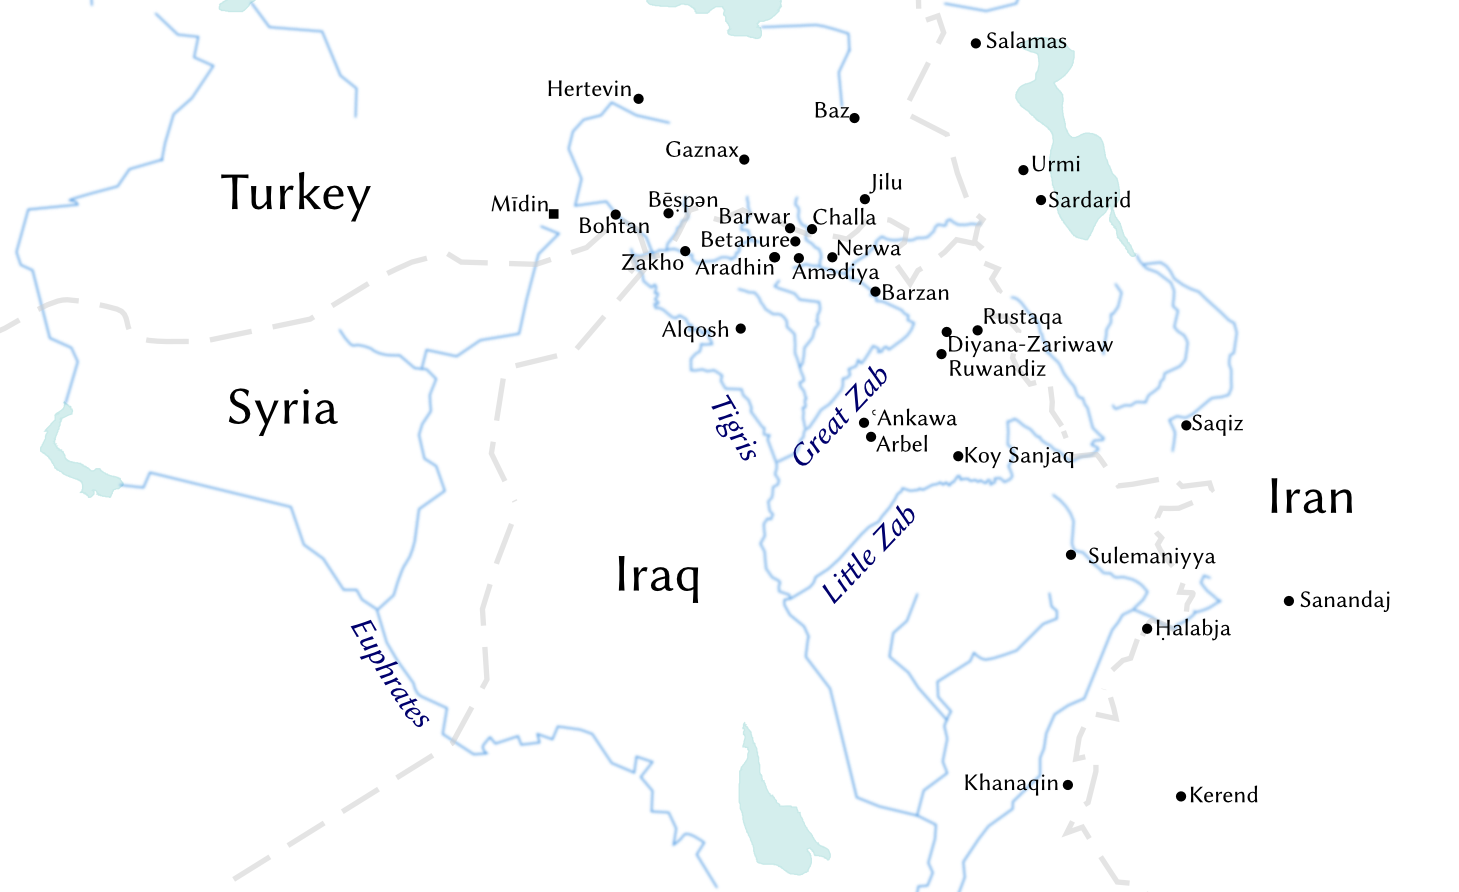
\includegraphics[width=\textwidth]{figures/NENAmap.png}
\caption{Approximate locations of NENA dialects (and one NWNA dialect: 
\Midn) at the beginning of the 20\th\ century.} \label{fg:map_nena}
\end{figure}


The amount of information gathered from the different sources varies considerably. Seven dialects (marked in \textbf{bold} in \ref{tb:dialects}) contributed each between 100 and 200 examples to the research database, together amounting  to two-thirds of the \ili{NENA} data-points in it. Not surprisingly, amongst these are the 4 dialects to which survey chapters are devoted. The remaining dialects contributed each between 8 to 60 examples each.  Data from the dialects of Khabur\il{NENA!Khabur dialects} \citep{TalayKhabur} were collected as well, but for methodological reasons are not treated in the book.


The data collected was registered in a Microsoft Access database. Accordingly, in this database all the various ACs found in the different \ili{NENA} dialects surveyed, as well as other  languages under investigation (mainly Kurdish and Syriac), were listed and linked to appropriate examples. The classification of the ACs in the database was done according to the principles outlined in \vref{ss:typology_here}. An example of the data-entry form is given in \vref{fg:ACform}. The database can be found online as part of \citet{GutmanThesis}.\footnote{In the electronic database the \prim and \secn fields are referred to as Nucleus and Attribute respectively.}

\begin{sidewaysfigure}[p]


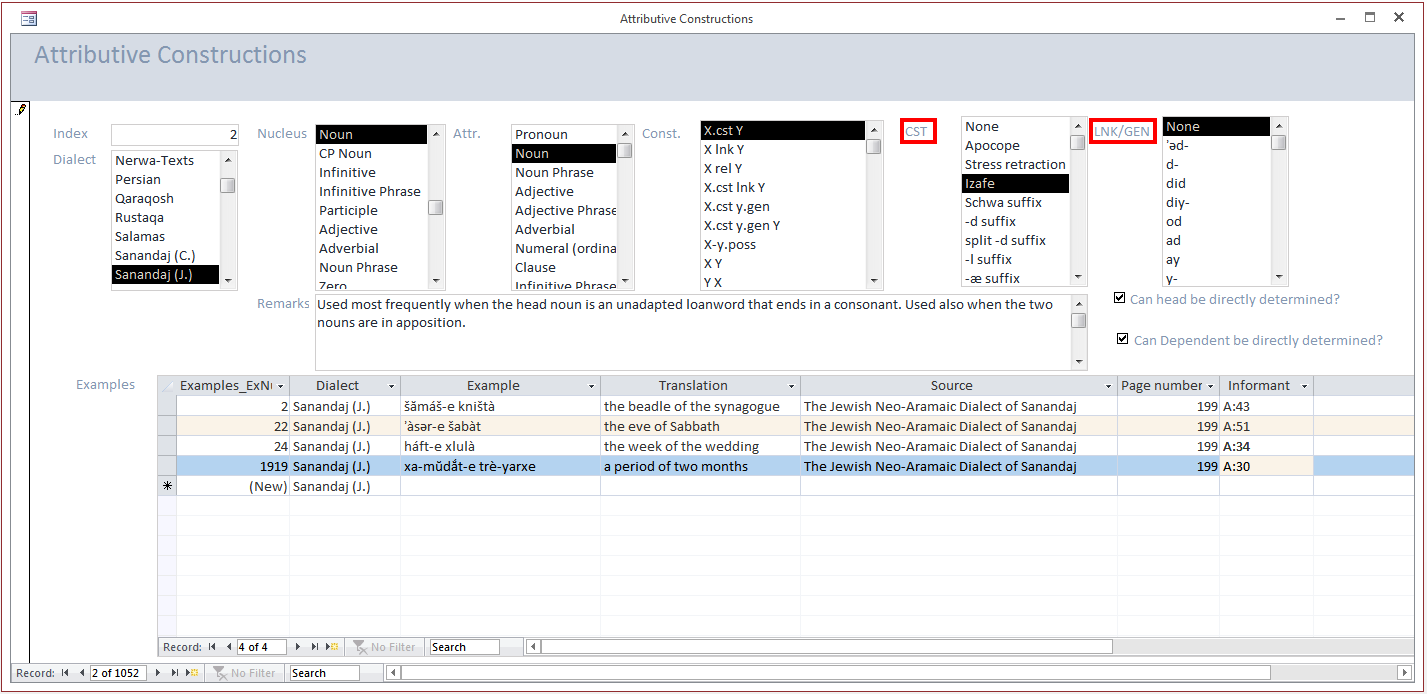
\includegraphics[width=\textheight]{figures/ACform.png}
\caption{Example of data entry in the accompanying database} \label{fg:ACform}
\end{sidewaysfigure}

 
While many of the consulted \ili{NENA} grammars have sections labelled \enquote{Annexation}, \enquote{Attributes} or the like, the concept of the \isi{attributive construction} as  defined in the current work is normally not described in any single section of the grammar, requiring collection of examples from numerous sections in a given grammar.\footnote{An exception is the grammar of \JZax, \citet{CohenZakho}.} The data assembly started with the collection of ACs headed by nouns modified by various attributes (nouns, adjectives, clauses etc.). Only subsequently were examples with other types of \prims (pronouns, adjectives, adverbials etc.)\ collected, yielding possibly a less systematic picture of these combinations. 

It should be noted that the listing of the different constructions is purely qualitative, as no quantitative data were gathered from the corpora. Thus, any remark regarding the usage frequency of a given construction is based on comments given in the consulted grammars.

The database design permits to query cross-dialectally the presence of a specific construction, with or without limitations to the parts-of-speech involved. This possibility was invaluable for conducting the comparative research, constituting the core of the current study (see chapters 10--11). 

\paragraph*{Format of examples} \label{ss:examples_format}
The \ili{NENA} examples given in this work are all taken from the database. While the database conserves the original transcription system of each source, in the book I have attempted to normalize the different transcriptions to a standard system, namely that of \citet{KhanBarwar, KhanSanandaj, KhanUrmi}.\footnote{Note that older publications of Khan, such as \citet{KhanArbel, KhanSulemaniyya} use a slightly different system. The main difference has to do with the transcription of a short \phonetic[ɪ]\~\phonetic[ə] vowel, which in later works is transcribed as \transc{ə}, while in earlier works it is transcribed as \transc{ĭ}.  Notwithstanding the question of transcription, it should be noted that not in all dialects is the difference between a tense \phonetic[i] and a lax \phonetic[ə] phonemic (see for instance the discussion of \Gaz phonemic inventory in \cite{GutmanGaznax}). Another change concerns the rendering in \ili{NENA} dialects of a fricative \phonetic[θ] consistently as \transc{θ} rather than \transc{ṯ}. Especially affected is the transcription system of \citet{YounansardaroudSardarid}, which I have simplified by removing the vocalic-timbre marks as well as most timbre superscripts \citep[cf.][20]{YounansardaroudSardarid}. The hard timbre which is marked by her as superscript \textsuperscript{h} is marked here with a ⁺ sign, in accordance with \citet{KhanUrmi}.}

 All examples have a title stating the language (or dialect) of the example as well as the categories of the members of the AC under discussion. Thus, a title of \textbf{Noun Phrase-Adjective} means that the example illustrates an AC with a noun phrase modified by an adjective, irrespective of the question of the ordering of the adjective and the noun phrase in the example itself, and the possibility of other (typically embedded) ACs appearing  in the example. The examples are glossed according to the Leipzig Glossing Rules \citep{LeipzigGlossingRules} with some additions (see list of glosses \vpageref{ap:glosses}). 
  
  Typically, the examples are cited using the source's page number where they are discussed (unless they are cited directly from a corpus). The original example number (if available) is given in parenthesis. If the author gives a reference to his own corpus (typically a letter+number combination), this is given in square brackets.
  
  The format of examples is illustrated \vpageref[below]{ex:example}.




\acex[Language]
{\Prim}{\Secn}{example}
{Example text}
{Glosses}
{Translation}
{}{(Source: page (example number) [Textual reference])}

  %add a percentage sign in front of the line to exclude this chapter from book
\chapter{Attributive constructions: Typological and Semitic perspectives}
\label{ch:attributive}
\largerpage
\section{Theoretical framework} \label{ss:theoretical_framework}

The current research, while informed by advances in \isi{linguistic typology}, is situated methodologically within the structuralist current of linguistics, which analyses language as a system of oppositions, be they between the consecutive constituents of  an utterance (the so-called \concept{syntagmatic axis}) or between possible constituents at a given point in discourse (the \concept{paradigmatic axis}). The usage of these analytical concepts will be further clarified below. While the structuralist tradition is interested mainly in the description of a single language, one can profitably extend these tools to compare and contrast several languages, as I do in the current study.

In structuralist linguistics, \concept{morphemes} are defined by way of opposition along the paradigmatic axis: Whenever an element of language (a \concept{signifiant} in Saussurian terms) stands in opposition in a given \concept{environment} (or \concept{syntagm}) with other elements and its exchange by these other elements co-varies systematically with a difference in \textit{meaning} broadly conceived (a \concept{signifié}), this element can be identified as a \concept{linguistic sign}. Minimal signs, i.e.\ those that are not analysable in terms of smaller signs, are considered to be \concept{morphemes}. As simple as this procedure is, it is possible to apply it in quite different ways, in accordance with the understanding of the term \concept{environment} used above. If by \concept{environment} one means a well-formed utterance, one gets the classical notion of a \concept{structural paradigm}. If, on the contrary, one allows for opposition within smaller environments, such as word-forms, the above procedure yields the notion of a \concept{morphological paradigm}. The elements identified as morphemes would be different in each case: For instance, a grammatical \isi{case marker} attached to a noun-stem, whose usage is obligatory in certain environments may not be considered a morpheme within the classical approach (as it does not stand in opposition within a well-formed utterance), but it can be seen as a morpheme in the morphological approach, as the word in isolation shows variation in case. In this study I opt for the latter approach: namely, morphemes are defined relative to word-forms in isolation, and not relative to full utterances.  

Linguistic structuralism is normally equated with no \textit{a priori} categories of language, as these should be defined on a per-language basis using the analytical method sketched above. Yet,  as this research follows the footsteps of previous scholars, I will operate within a framework assuming the existence of three general grammatical relations in language, described in the next section. Of these, the \concept{attributive relationship} shall be seen as the abstract functional correlate of the concrete grammatical patterns examined, the \concept{attributive construction}\textsc{s} (ACs). This is further explained in \ref{ss:attr_relation}. In structural terms, the \isi{attributive relationship} is the \concept{signifié} 
of several different \concept{signifiant}\textsc{s}. 

The rest of the chapter is devoted to anchoring these terms in the traditions of \isi{linguistic typology} (\ref*{ss:AC_typ}) and of \ili{Semitic} linguistics  (\ref*{ss:AC_sem}). \Ref{ss:typology_here} synthesizes from these different approaches one methodology used in this study. 

\subsection{The three relations} \label{ss:threeRel}

In this book, I rely on a simple dependency model of morpho-syntax admitting three basic dependency relations holding between elements of a clause: 

\begin{enumerate}
\item The \concept{predicative relation}, holding between a subject and a predicate.

\item The \concept{attributive relation}, holding between a head and its attribute.

\item The \concept{completive relation}, holding between a predicative construction and a complement.
\end{enumerate}

This theory, as presented here, was advocated by the Israeli linguist Gideon Goldenberg (1930--2013), who himself credited the German philologist Karl Ferdinand Becker (1775–1849) as being one of its early forefathers \parencites(see)()[10]{BeckerGrammar}{GoldenbergRelations}[Ch.\ 11]{GoldenbergSemitic}[37--38]{CohenSha}{GutmanReview}. 

Goldenberg saw the theory as both general in scope and at the same time especially adequate to the \ili{Semitic} family:\footnote{Goldenberg clearly saw these relations as valid cross-linguistic notions, but he  did not address the question whether they represent linguistic universals, nor did he tie them to any nativist conception of language. It seems, rather, that  the cross-linguistic validity of these notions stems from the fact that they represent syntactic correlates of necessary communicative functions of language such as assertion (the \isi{predicative relation}), qualification of referents (the \isi{attributive relation}) and of events (the \isi{completive relation}).} 

 \blockquote[{\citealt[142]{GoldenbergSemitic}}][.]{The recognition of three essential types of grammatical relations, or bonds, has been a major approach to syntactic analysis commonly pursued in linguistics during the last two centuries. With regard to \ili{Semitic} languages and in connexion with case declension such a conception appositely reflects the very structure of the languages involved} This is so, since the case-marking classical \ili{Semitic} languages (\CArab, \ili{Akkadian} and \ili{Ugaritic}) have exactly three cases, which correspond well with the three mentioned relations. Regarding linguistic change in \ili{Semitic} languages, he asserted that by using this theory  \blockquote[{\citealt[142]{GoldenbergSemitic}}][.]{we may be able to better understand the meaning of changes in some innovative languages and thus perhaps even to measure typological innovation}. Since the aim of this book is exactly to investigate change in modern \ili{Semitic} languages, namely the \ili{NENA} branch, the usage of this theory seems especially adequate. 

To the three above-mentioned dependency relations, one must add \concept{apposition}, not being a dependency relation, but rather an equivalence relation. In this framework, two elements are considered to be in \concept{apposition}, whenever both are governed by the same dependency relation, share potentially the same grammatical features (number, gender, case and \isi{definiteness} -- if explicitly marked), and are co-referential. In such conditions, they can replace each other syntactically, although the two may not be equivalent on semantic and discursive grounds, as one element may take a higher information load. In the latter case, my notion of \isi{apposition} is similar to the notion of \enquote{appositional modification} defined by \citet[13]{Riessler} as following: \enquote{Semantically, the appositional modifier is headed by the modified noun.
Syntactically, however, the appositional modifier has an empty head which is
co-referential with the \isi{head noun} of the apposed noun phrase.} His \enquote{empty head} is analysed in the current framework as a covert pronominal element.\footnote{See also Cohen's definition of \isi{apposition} given in \vref{ft:Cohen_Apposition}. \citet[65]{Acuna-Farina1999} rejects a similar notion of \isi{apposition} claiming that \enquote{[i]f a syntactic relationship of this type is to be posited, then that relationship must be applicable to a number of other constructions, and
not just to one construction}, and contrasts it with the widely applicable notion of dependency. Yet, in the current framework, \isi{apposition} is not a syntactic relation \textit{sensu stricto}, i.e.\ a dependency relation, but rather an equivalence relation. Compare again with \citet[38]{CohenSha}: \enquote{It must be stressed that \isi{apposition} [...] is not in itself a relationship, but rather a repetition of a syntagm, and occasionally, of the relationship itself.} As such, the notion of \isi{apposition} is applicable to a wide range of constructions.}

\subsection{The attributive relationship and its manifestation}
\label{ss:attr_relation}

In this book, I am interested only in one of the relations mentioned above, namely the \concept{attributive relation}. This is the dependency relationship within the NP domain which holds between a \isi{head noun} (or pronoun) and a second nominal element (the \concept{attribute} or \concept{dependent}) qualifying the \isi{head noun} \parencites(cf.)()[1--2]{GoldenbergAttribution}{CohenAttribute}. This notion is closely related to Jespersen's notion of \concept{junction} \citep[Ch.\ 8]{JespersenPhilosophy}. Note that semantically, there is no restriction on the type of the qualification involved, which may range from possession to qualification of some property of the head. 



In structuralist terms, the \isi{attributive relation} is a \concept{signifié} (function) whose \concept{signifiant} (form, i.e.\ morpho-syntactic exponent), is  an \concept{attributive construction} (=AC).
 I use the term \concept{construction} here as denoting a linear ordering of segmental (and possibly super-segmental) material together with paradigmatic slots, \enquote{place-holders} so to speak, which can accommodate either an open group of elements (i.e., a lexical paradigm, often corresponding to some part of speech), or a closed group of elements (i.e., a functional paradigm, often corresponding to an inflectional paradigm of some morpheme), to which a specific function is tied.\footnote{The notion of \concept{construction} was popularized by the proponents of Construction Grammar \citep[e.g.][]{GoldbergConstructions,CroftRadical}. It corresponds in fact to an abstract understanding of the long-standing Saussurian notion of \concept{linguistic sign}, i.e. a coupling of \concept{form} and \concept{function}.} In a given language, one may find many different attributive constructions. While all of these encode an \isi{attributive relationship}, they may be  used in different syntactic contexts, or convey different semantic or stylistic nuances. I will only linger upon these differences as far as they are insightful for my comparative purposes. 

Every AC is defined as having two paradigmatic slots corresponding to the head and the attribute. In some cases, however, the two elements in question are split across two separate NPs which stand in \isi{apposition} to each other, rather than in an \isi{attributive relationship}.   In such a configuration, it is often the case that the \isi{attributive relationship} holds within one of the NPs, in which the other NP is being represented pronominally. In virtue of this, it is possible to identify one NP as being the qualified, and the second NP as being the qualification,\footnote{It is often the case that the qualifying NP follows in discourse the qualified NP, in accordance with the general tendency of pronouns to be anaphoric rather than cataphoric.} and posit an \concept{indirect attributive relationship} between them (cf.\ the term \concept{indirect annexation} used by \cite[79]{GoldenbergEarly}).
Yet  in such a case one cannot accurately use the terms \emph{head} and \emph{attribute}\is{attributive} for these NPs, as they imply a direct \isi{attributive relationship} between the two elements. To overcome this terminological problem I shall use the notions of \concept{primary} and \concept{secondary} to denote the two members, in line with \citet[38]{PlankIntro}:\footnote{These terms clearly bear affinity to the same terms introduced by \citeauthor{JespersenPhilosophy}, but note that his usage is broader, as it applies equally well to cases of junction as well as nexus \citep[97]{JespersenPhilosophy}.}

\blockquote{The nominals in relation will be neutrally referred to as \concept{primary} and \concept{secondary}. Attributes are prototypical secondaries
vis-a-vis their heads [...] but on referential and distributional grounds, secondary rank is also justified for the appositum in \isi{apposition} or for a nominal indirectly related to
another as a secondary predicate or the like.}

Prototypically, the \prim and the \secn are expected to be nouns, but this does not exclude other nominal elements, chiefly pronouns and adjectives. Moreover, as we shall see, the \secn can also be  a \isi{prepositional phrase} (a PP), or even a clause (Cl). Moreover, in \ili{Semitic} languages the same constructions are often used with \isi{adverbial} elements (prepositions or conjunctions) as \prims. While these uses can be seen as peripheral, and not strictly realizing an \isi{attributive relationship}, they are sometimes illuminating for the study's comparative purposes, and thus will be taken into account.



\section{Attributive constructions from a typological perspective} \label{ss:AC_typ}
\largerpage
The notion of the \isi{attributive relationship}, and the corresponding ACs,  is clearly a very broad, unifying concept. Many typological studies, on the other hand, look at a restricted set of ACs as their object of study. Thus, \citet{UltanPossession} establishes a typology of \concept{possessive constructions}, i.e.\ ACs whose \secn is a nominal possessor.\footnote{Ultan elaborates a quite complex typology, taking into account both the \concept{locus} of marking (see \sref{ss:head_vs_dep}), and the type of marking: whether it is syntactic or morphological on the one hand, and whether it indexes features of the possessed noun or the possessor. Yet  at the end he reduces this typology to a simple \concept{locus} typology. Unfortunately, the lack of clear definitions of the various marking categories and the sparse use of examples renders his work less than insightful.}  More recently, \citet{Tamm2003Possessive} discusses the \textit{Possessive noun phrases in the languages of Europe}. A similar restriction is taken by \citet{NicholsBickelWals}, discussed further below. The restriction applied is basically a semantic one. Another quite common division of the domain of ACs is according to the syntactic category of the \secn: Dryer, looking at word-order phenomena, separates ACs whose \secn is a noun (a \enquote{genitive}), an adjective or a \isi{relative clause} \citep{DryerWALS86, DryerWALS87, DryerWALS90}. \citet{GilWals60}, on the other hand, examines to what extent these three categories are differentiated across the languages of the world.\footnote{\citet[235]{GoldenbergSemitic} comments on Gil's approach: \enquote{[t]he constitutional identity of constructions with genitive nominals, adjectives, and relative complexes will in any case belong to the profoundest level of language structure, not to be regarded as different semantic types of attributions that collapsed due to imperfect differentiation}. }



\newpage 
In the framework of Canonical Typology, \citet{NikolaevaSpencer} pose inalienable possession and attributive modification (by adjectives) as two separate canonical constructions,\footnote{Note that their use of the term \concept{construction} is different than ours, as it is not tied to a specific manifestation in language.} while alienable possession and modification by noun are their non-canonical counterparts. While they too split the AC domain, using both  semantic and syntactic criteria, they do acknowledge that \textquote[{\cite[209]{NikolaevaSpencer}}]{there is some deeper link between the two constructions}, by examining languages in which these functions are expressed identically, specifically the {Ezafe} marking of \ili{Iranic} languages (which shall be examined carefully in this book; see \sref{ss:ezafe_dispute}).

It is not surprising that large scale typological studies attempt to focus on a restricted domain of constructions, using various semantic and syntactic criteria to delimit it. Such criteria, in line with Haspelmath's notion of \concept{comparative concept}\textsc{s} \citep{HaspelmathComparative}, assure the typologists they are comparing like with like. As this study is focused on a restricted and similarly shaped set of languages (namely, the \ili{NENA} languages and their contact languages), I have had the leisure of defining a broader object of study. Of course, more comprehensive accounts can be found in the typological literature as well. Thus, \citet{Fairbanks} starts by treating equally cases of adnominal modification by nouns, PPs and clauses, although his main interest is nominal modification. Another broad account,  discussed in more detail below, is that of \citet{PlankIntro}.

In the following, I shall examine in more detail the typologies of \citet{NicholsBickelWals} and \citet{PlankIntro}. To round of the picture, I shall present also the recent typology elaborated by \citet{Riessler}.

\subsection{Head-marking vs.\ dependent-marking typology} \label{ss:head_vs_dep}
\largerpage[2]
Following the pioneering work of \citet{NicholsHead},  \citet{NicholsBickelWals} classify possessive constructions (and subsequently languages\footnote{For each language, they consider only one construction, which \enquote{is [the] default or has the fewest restrictions} \citep[\S 2]{NicholsBickelWals}.}) according to the \concept{locus} of marking, i.e.\ whether the construction is marked morpho-syntactically on the head (\prim in the current terminology) or the dependent (\secn), irrespective of the order of these two constituents.\footnote{Such a classification has in fact been proposed earlier by \citet{UltanPossession}, but in less clear terms.} Since the marking of each \isi{locus} is independent, this simple typology yields 4 types of marking: \isi{head marking}, \isi{dependent marking}, \isi{double marking} and no marking.\footnote{A fifth category, is dedicated to \enquote{low-frequency but systematic further patterns} \citep[\S 1.5]{NicholsBickelWals}. These are cases where the markers could not be easily associated with either the head or the dependent, but they represent only 2.5\% of their sample (i.e.\ 6 languages).} 

\newpage 
While this typology succeeds  at capturing large geographical distributions, it suffers from two shortcomings rendering it somewhat simplistic at the descriptive level. 

First, there is no differentiation between syntactic marking and morphological  marking. Rather, the authors agglomerate the two under the heading \enquote{overt morphosyntactic marking}.\footnote{By syntactic marking I mean marking achieved by a separate syntactic element, typically bearing phrasal scope, while morphological marking is achieved by inflection of a word, possibly (but not necessarily) having narrow scope on that word only. Recently, \citet{HaspelmathWord} has suggested that this distinction is void and cannot be applied consistently across various languages, yet I find it important in studies of \isi{language change}, like the current one.} 
Thus, the preposition \transc{of} in the \ili{English} phrase \transc{the price of oil} is considered to be a case of dependent-marking, probably due to its syntactic co-constituency with the dependent, on par with an inflectional genitive \isi{case marker}.\footnote{Cf.\  \citet[36]{Fairbanks}: \textquote{The main distinction between the genitive inflection and the pre/postposition is that the genitive inflection is inseparable from its noun and it must be repeated in certain situations.}} Since the syntactic constituency of an element may be disputed in some cases (especially if it cliticizes to another element), this can lead to analytical difficulties.\footnote{Indeed, as we shall see in \sref{ss:ezafe_dispute}, such a controversy exists around the \Per \ez* particle. \citet{NicholsBickelWals}  classify it without further comment as a head-marking instance.} 

Secondly, the typology does not differentiate between two quite distinct types of markers:  pure relational markers versus pronominal markers, which represent the antipodal \isi{locus} (i.e.\ the opposite member of the construction). Thus, in \ili{Turkish}, in which one finds both head marking and dependent marking, the two markers are of quite distinct type:


\acex[\Turk]
{Noun}{Noun}{Turk1}
{çocuğ-\opt{un} araba-sı}
{child-\opt\gen{} car-\poss.3 }
{\opt{the} child's car}
{Bozdemir}{49}

\largerpage
The dependent-marker is purely relational (a \isi{genitive case}),\footnote{The usage of the \isi{genitive case} in \ili{Turkish} is in fact not obligatory. When it is used it usually marks the \secn as definite and specific. In this it is similar to \ili{Turkish} \acc* case, which marks only definite objects. See \citet[49f.]{Bozdemir}.}  while the head-marker is pronominal. This is crucial, since the expression \transc{araba-sı} is by itself a well-formed NP meaning \transl{his car}. A similar criticism is made by \citet[229]{GoldenbergSemitic}:\blockquote{Attributive, or possessive, syntactic relations are commonly regarded as being marked either on the head or on the dependent attribute, not only by stem form or case, but also by personal morphemes, as if the possessive relation in \enquote{the man \textsuperscript{his-}house} (for \enquote{the man's house}) is marked by \enquote{his} on the head term \enquote{house} [\ldots] Pronominal morphemes, however, like other nominals or nominalizations, are not markers of the head-dependent relation, but belong with the \textit{termini} [=loci\is{locus}, \prim or \secn{}] between which the relation is apprehended.}

These two shortcomings were addressed to some extent by a more elaborate typology, presented in the next section.

\subsection{Plank's adnominal typology} \label{ss:Plank_typology}

A more elaborate typology of adnominal modification is presented by \citet{PlankIntro}. It is not restricted to a specific semantic domain of ACs, and indeed no specific restrictions are put on the \secn, except it being of nominal nature. As \citet[38]{PlankIntro} puts it: \blockquote{The following taxonomy of marking patterns is therefore
intended to be neutral (a) as to whether the nominal to be related to
another is a noun or something else (such as a derived adjective), and (b) as to
whether its relationship is one of [direct] attribution or of some other kind (such as
\isi{apposition}) --- and indeed, whether this relationship is that of an immediate
adnominal constituent or not.}

As mentioned above (\sref{ss:attr_relation}), Plank re-introduces the terms \textsc{primary} and \textsc{secondary} to refer to the two nominal members of the construction, which he symbolizes as X and Y, a practice I shall follow below.

Disregarding the word order of the two elements, Plank opts for an elaborate head vs.\ dependent marking typology, in which he differentiates between pure relational markers and pronominal markers, which he calls \concept{relatedness-indicators}.\footnote{I use here the term \emph{pronominal} in the basic meaning of representing (and possibly substituting) a noun.
In a similar typology proposed by \citet[ch.\ 2]{Riester}, such markers are termed \concept{agreement markers}. Riester's  typology is further elaborated in that it distinguishes between \concept{local agreement}, i.e.\ a marker exhibiting features of its own constituent, and \concept{non-local agreement}, i.e.\ a marker exhibiting features of the other constituent. Only the latter would be considered \concept{relatedness-indicators} in Plank's system.} 

\begin{modquote
The
relations identified may be those of secondary [pure \isi{dependent marking}] or of primary [pure \isi{head marking}]
 or of both [pure \isi{double marking}], with the markers normally associated, morphologically
or syntactically, with the respective nominals themselves. Relatedness-indicators
may occur on the secondary [pronominal dependent marker], reflecting some property of the
primary that it belongs with (such as its number, gender/class, person, or case);
or they may be on the primary [\isi{pronominal head} marking], reflecting some property of the secondary that it belongs with, or on both [pronominal \isi{double marking}]. {\citep[38]{PlankIntro}}
\end{modquote}

Since each one of the 4 markers type is in principle independent of the others, this yields 16 construction types. In fact, in the case of no marking at all, Plank distinguishes between syntactic \isi{juxtaposition} of the \prim and \secn (X\#Y), and morphological compounding of them (X+Y). However, except for this distinction, and judging from the citation above, syntactic and morphological markings are considered alike.\footnote{Thus \citet[656]{Tamm2003Possessive} commenting on Plank's work, writes: \enquote{[this] taxonomy does not distinguish morphological boundedness and syntactic association.}}
Plank acknowledges, however, the possibility of a third \isi{locus} of marking, namely \textquote[{\cite[39]{PlankIntro}}]{markers of the entire construction, linking
primary and secondary without forming a morphological co-constituent of either [...] (\enquote{associative} markers or lexical items such as `thing', `possession/belong', 'place')}. He dubs these items \enquote{links}. The elements may themselves carry pronominal markers of the \prim, the \secn or both, adding 4 more construction types.\footnote{He does not list construction types where both the link and the \prim or \secn are marked. If all these combinations would be marked, there would be 64 construction types. }

\textit{Prima facie}, one would expect such \enquote{links} to form a syntactic co-constituent with the \secn (see \ref{ss:Analytic_AC}), so it is not  clear what distinguishes them from normal secondary marking in Plank's typology.\footnote{Indeed, later on Plank acknowledges this difficulty: \textquote[{\cite[51]{PlankIntro}}]{No 7. [X Y-sec-x], [is] not always easily distinguished from No. 17, X Link-x Y}. \label{ft:lnk_difficulty}} Examining the accompanying examples does not clarify this point. Notwithstanding this possible confusion, Plank's typology is important in that it raises the question of distinguishing morphological marking vs.\ syntactic marking, and more importantly, it makes a clear difference between pronominal markers and pure relational markers. The typology adopted in this study is based to a large extent on Plank's typology. 

\largerpage[-1]
\subsection{Rießler's typology of attribution marking}


\begin{table} 
 
\begin{tabular}{l l}
\toprule
Juxtaposition & $X\ Y$ \\

Incorporation & $X+Y$ \\

Linker & $X\ \lnk\ Y$ \\

Anti-\isi{construct state} & $X\ Y_{\textsc{anti-cst}}$ \\

Anti-\isi{construct state} agreement & $X\ Y_{\textsc{anti-cst+agr}}$ \\ 

Construct state & $X_{\cst}\ Y$ \\

Double construct & $X_{\cst}\ Y_{\textsc{anti-cst}}$ \\

Head-driven agreement & $X\ Y_{\agr}$ \\

Possessor agreement & $X-y_{\poss}\  Y$ \\

\bottomrule
\end{tabular}

\caption{Rießler's typology of attributive marking}\label{tb:Riessler_typology}
\end{table}



As a last point of reference, I shall examine a recent typology of attribution marking elaborated by \citet[Ch.\ 4]{Riessler}. While Rießler focuses on \isi{adjectival attribution}, his typology covers larger ground, and is thus relevant for this study. In many respects, Rießler's typology is equivalent to Plank's typology discussed above, except that he uses a more technical, and to some extent obscure, terminology.\footnote{Judging by the lack of citation of \citet{PlankIntro} in Rießler's work, it seems his typology was elaborated independently of Plank's work.} I discuss it here, nonetheless, in order to compare the current framework (derived by and large from Plank's) to another recent typological framework of the same domain.

\citet[62]{Riessler} considers three main dimensions which characterize attributive markers, quoted hereby:

\begin{itemize} 
\item \textit{Syntactic source}, i.e., the central syntactic operation which constitutes attribution
and belongs either to \textit{agreement marking} or \textit{government}. [...]

\item \textit{Syntactic pattern}, i.e., devices projecting adjective phrases versus devices
projecting full noun phrases [...]

\item \textit{Syntactic \isi{locus}} of the respective formatives.
\end{itemize}


\largerpage[-1]
By \textit{syntactic source}, Rießler refers to the same distinction which Plank made between relational markers and (pronominal) relatedness markers. Pure relational markers are qualified by him as being issued by \enquote{government} of the entire construction ([+ \textsc{gov}] in his terminology), while relatedness markers are exponents of agreement ([+ \agr]). In cases where both marker types accumulate on one member, such as Plank's [X Y-sec-x] construction, he sees the agreement as being \enquote{secondary}.\footnote{In a quite unfortunate terminological decision, Rießler terms the pure relational markers \enquote{construct state} markers, whether they appear on the head or on the dependent (in which he calls it \enquote{anti-construct state}). As we shall see in the next section, the \isi{construct state} category is better reserved for use as a head-marking device, while the notion of \concept{case} should be used for dependent-marking. It seems that Rießler is reluctant to use the term \enquote{genitive case} to term the dependent-marking relational marker since he associates it with possessive semantics and his work focuses on \isi{adjectival attribution} \citep[see][43]{Riessler}.}

The second dimension, \textit{syntactic pattern}, is a novelty of this typology. Note, however, that it is specific to \isi{adjectival attribution}, and moreover, it assumes that there is a clear distinction between adjective phrases and (full) noun phrases. As we shall see  in \sref{ss:Goldenberg_typology} below such an assertion is not evident for the \ili{Semitic} languages which are the object of the current study.

The third dimension, \textit{syntactic \isi{locus}}, refers to the position of the marker: either on the head or the dependent. Just as Plank (and following \cite{NicholsHead}), \citet[59f.]{Riessler} recognizes a third \enquote{floating} locus of marking, not associated with any member of the construction. He terms such markers \enquote{linkers} and brings the Tagalog \transc{na/-ng} attributive marker as an example.\footnote{This marker appears in the second position of the NP, irrespectively whether the NP has the order attribute+head or head+attribute.} Interestingly, he notes that such true \enquote{linkers} are not found within his survey of the languages of northern Eurasia (see in this respect \vref{ft:lnk_difficulty}).

Rießler does not in general classify the markers according to their binding nature (syntactic or morphological), though interestingly, just as Plank he distinguishes between syntactic \isi{juxtaposition} (Plank's X\#Y) and morphological incorporation (Plank's X+Y) \citep[29--32]{Riessler}.

Using these different criteria, Rießler elaborates a typology of 11 different \isi{attributive construction} types (not counting \isi{double marking}). Disregarding those which are specific for \isi{adjectival attribution}, the remaining constructions are presented in \vref{tb:Riessler_typology}, alongside with an adaptation of Plank's notation for these constructions. This table can be compared to \vref{tb:main_AC_strategies} which presents the \isi{attributive construction} labels used in this study.

\section{Attributive constructions from a Semitic perspective} \label{ss:AC_sem}

In the \ili{Semitic} language family, the typical attributive construction is the \concept{annexation} construction, or \concept{construct state construction} (=CSC),
 in which the \prim  is marked by a special morphological form, the \concept{construct state}.\footnote{The use of the term \concept{construct state} alone to name the construction is thus misleading. Unfortunately, such a usage is prevalent in certain formal schools of linguistics, and even made it way to the Encyclopedia of \ili{Arabic} Language and Linguistics \citep{BenmamounConstruct}.} In \ili{Semitic} grammars, the \prim in this construction is normally called \concept{nomen regens}, and the \secn \concept{nomen rectum}, but I will stick to the terms \prim and \secn. 


\subsection{Relational nouns and the category of state} \label{ss:state}

In \ili{Semitic} languages, nouns (as well as other nominals) are inflected not only for the familiar categories of \textsc{number}, \textsc{gender} and possibly \concept{case}, but also for the category of \concept{state} \parencites(cf. for \ili{Hebrew})()[579]{HeckeConstruct}[581]{DoronConstruct}. In contrast to the other categories, the category of state is not \concept{projecting}, i.e.\ it is invisible for elements outside the NP in which it occurs. It may be for this reason that it has often been ignored in linguistic studies as a fundamental morpho-syntactic category of language, although it is in fact not restricted to \ili{Semitic} languages.\footnote{But see \textcites[344]{RetsoState}[268, especially fn.\ 3]{RetsoPlural}, who treats the notion of state as a morphological category in \ili{Semitic} languages, albeit as representing \enquote{allomorphic variation}, as he relies on the notion of \isi{structural paradigm}s (see \ref{ss:theoretical_framework}). The converse position, denying the validity of the category of state, is  advocated by \citet[318]{FaustAt}, who claims that the \isi{construct state} is \enquote{not a primary linguistic notion}.} 

Basically, the category of state encodes the \concept{syntactic valency} of a noun, i.e.\ whether it must be followed by a complement or not.\footnote{Semantically, this complement may be conceived as a mandatory argument of some sort of the noun, or as an adjunct qualifying the noun, but this distinction is neutralised syntactically. Of course, from a syntactic view point, a mandatory adjunct is \textit{de facto} an argument. } 

It is instructive to contrast this phenomenon with the notion of \concept{semantic valency} of nouns, i.e.\ the number of argument they have in their semantic structure. It is a well known fact of language that some nouns (like \textit{man}) can appear by themselves, while others (e.g.\ \textit{son}) conceptually require some specification. \citet[8]{BarkerPossessive} calls the second group \concept{relational nouns} and the first  \concept{non-relational nouns}. The relational nouns are particular in that they denote relations over pairs of referents, while the non-relational denote simple referents \citep[see also][216f.]{NikolaevaSpencer}. In terms of \isi{valency}, the relational nouns are semantically bi-valent, while the non-relational are semantically mono-valent (counting the referent of the noun itself as one argument). In many languages, this semantic  difference is not related to any morpho-syntactic category. Other languages do mark the difference. One common possibility cross-linguistically is to encode the difference of \isi{valency} by distinguishing two classes of nouns, namely alienable vs.\ inalienable nouns, the latter representing relational nouns mandatory complemented by a possessor. For instance, in the American Navajo language the root \foreign{-beʾ}{milk} cannot appear by its own, but must be possessed: \foreign{bi-beʾ}{her milk (from her breasts)} or \foreign{ʾa-beʾ}{something's milk} \citep{BickelNicholsWals58}.

In contrast to languages which mark semantic \isi{valency}, which is inherent to the nominal lexeme, \isi{state morphology}, marking syntactic \isi{valency}, encodes \textit{ad-hoc} whether in a given context a noun should be understood as relational (i.e.\ requiring a complement) or as potentially non-relational (self-sufficient).\footnote{As the non-relational form is the unmarked form it does not exclude the possibility for a noun to receive a complement. Indeed, inherently relational nouns, such as kinship terms, may still appear in the non-relational form in languages with \isi{state morphology}. Note also that in \ili{Semitic} languages the \cst* applies as well to other nominal elements (such as adjectives or numerals) when they are mandatory accompanied by a complement. It is important to stress  that in such a system inherently relational nouns (inalienable nouns) are not distinguishable morpho-semantically from non-relational nouns.  This is clearly stated by \citet{PatElInalienable} for \BHeb. The claim to the contrary of \citet{SiloniInalienable} regarding the existence of a syntactic class of inalienable nouns in \MHeb is factually wrong, as their alluded ungrammatical or infelicitous examples are neither ungrammatical nor infelicitous.}  The former is marked by the \concept{construct state}, while the latter is marked by the \concept{free state},\footnote{Some authors use the traditional term \concept{absolute state} as opposed to \isi{construct state}. Apart from being less self-explanatory, this term is problematic in the context of Aramaic, as will be explained below.} which is typically also the citation form of a noun.\footnote{A similar proposal, cast in a more formal apparatus, is given by \citet{HellerPossesion}. Heller sees \isi{construct state} nouns as denoting functions from individuals to individuals, in contrast to \isi{free state} nouns which denotes individuals.} By way of analogy, the \isi{construct state} is the nominal parallel of causative morphology in verbs: both add one syntactic argument to the argument structure of their host.

In light of the above, it is clear why the state category is non-projecting. In contrast to case, which signals what kind of dependent a noun is, and therefore should be accessible by constituents outside the NP, the \isi{state morphology} determines whether a nominal governs another nominal NP-internally, and therefore is invisible outside the domain of the NP. Intrinsically, \isi{state morphology} is a head-marking device. 

Thus defined, it is clear that the \isi{construct state}, or rather \isi{state morphology}, is not a phenomenon restricted to \ili{Semitic} languages. In this vein, \citet[74]{CreisselsConstruct} proposes to use the notion of \concept{construct form} \blockquote{as a general label for noun forms that are obligatory in combination with certain types of noun dependents and cannot be analyzed as instances of cross-referencing in the genitive
construction}.\footnote{\citeauthor{CreisselsConstruct} prefers the term \concept{construct form} over construct state due to the confusion arising from the use of the former as a construction label. I shall stick to the traditional term, but note that the notion of \concept{construct state} can relate both to the morphological marking, and to the syntactic position of a \prim (not necessarily marked as such). When in doubt, I will use the term \enquote{construct state marking} or \enquote{construct state form}.} Such a definition equates the \isi{construct state} with the primary relation marker of \citet{PlankIntro}.\footnote{An alternative term, proposed by \citet[268]{DixonBasicII} is \concept{pertensive}  \enquote{based on the \ili{Latin} verb \textit{pertinēre} ‘to belong’}. The term has not gained wide usage, as far as I am aware of. 
Dixon uses this term, moreover, as designating both simple markers and pronominal  markers. It may be for this reason that he does not simply adopt the notion of \cst*, although he is aware of the partial equivalence between the two \citep[310, fn.\ 16.2]{DixonBasicII}. I am grateful to \name{Adam}{Pospíšil}, who drew my attention to this term.}  \citeauthor{CreisselsConstruct} goes on to identify \isi{construct state} forms in a variety of African languages, ranging from \ili{Nilotic languages} in the east to \ili{Wolof} in the west. 

A terminological word of caution is appropriate here. Notwithstanding the above conception of the \cst* notion, it should be noted that in grammars of pre-modern Aramaic a three-way state distinction is given, opposing \concept{absolute state}, \concept{emphatic state} and \concept{construct state}. Both the \isi{absolute state} and the \isi{emphatic state} are in fact instances of the \isi{free state}, as defined above, and the opposition between them is related to the domain of determination: In the earliest stage of Aramaic, the \isi{emphatic state} was used to mark nouns as definite (as early forms of Aramaic lack a syntactic \isi{definite article}; see \sref{ss:intro_NPstructure}),\footnote{For possible origins of the \isi{emphatic state}, unique to Aramaic among \ili{Semitic} languages, see \citet{KönigEmphatic}.} while the \isi{absolute state} was in general used to mark nouns as indefinite. In this setting, the three-way state distinction is justified, in that a \isi{construct state} noun is by itself not determined, but rather the entire CSC inherits its determination feature from its \secn (see \sref{ss:CSCdet}). With time, the definite value of the \isi{emphatic state} was eroded, and it became the default form of the free noun, the \isi{absolute state} being restricted to specific syntactic contexts \parencites{JastrowDetermination}[22, \S 18]{MuraokaSyriac}. 


\subsection{The construct state construction across Semitic languages} \label{ss:cst_Semitic}

From the above discussion it should be  clear that the CSC is essentially a head-marking construction\is{head marking},\footnote{In the \ili{Semitic} languages which mark case, namely \ili{Akkadian} and \CArab, it is a double-marked construction\is{double marking}; see discussion further down in this section.} as in the following \ili{Hebrew} example (contrast with \foreign{\texthebrew{בַּיִת} bayiṯ}{house.\free}):

\hebacex[\BHeb]
{Noun}{Noun (Head-marked AC)}{heb_a}
{בֵּית הַמֶּלֶךְ}
{bēṯ ham-mɛlɛḵ}
{house.\textbf{\cst} \definite-king}
{the house of the king}{}

In \ili{Hebrew} the \isi{construct state} nominals are characterized by \enquote{lighter vocalisation} in comparison with their corresponding \isi{free state}. Sometimes they are marked by specific suffixes, namely \transc{-aṯ} for \fem* \sg* nouns (in contrast to free form \transc{-ā}) and \transc{-ē} (\MHeb \transc{-ey}) for \masc* \pl* nouns (in contrast with \transc{-īm}). All these changes can be  explained by the  \prim losing word stress, and forming one phonological word with the \secn \citep[580]{HeckeConstruct}. This explanation, however,  is diachronic, as in Modern \ili{Hebrew} these forms prevail even when the \prim gets its own stress, as is evident from cases where two \cst* \prims are conjoined:\footnote{In \BHeb it is generally accepted that only one nominal can occur as \prim, as the counter-examples are extremely rare \citep[210]{VerhejGenitive}: \citet[433, \S 128a, note 1]{Gesenius} lists 4 such tentative cases, of which only one is really clear (Ezekiel 31:16): \foreign{\texthebrew{מִבְחַר וְטֽוֹב־לְבָנוֹן} [miḇḥar wə tō̱ḇ] ləḇānōn}{the choice and best of Lebanon} (King James translation). Yet  one finds other cases of intervening material between a \cst* \prim and its \secn; see \citet{FreedmanBroken}. In \Syr too there is a rare occurrence of conjoined \prims; see \example{1009}. Similar examples are attested in Standard \Arab \citep[138f.]{BadawiCarter}.} 

\hebacex{Conjoined Nouns}{Noun Phrase}{MHeb_conj}
{מורֵי ותלמידֵי בֵית הספר}
{[mor-ey ve\cb{} talmid-ey] [bet ha-sefer]}
{teacher-\mpl.\cst{} and\cb{} pupil-\mpl.\cst{} house.\cst{} \definite-book}
{teachers and pupils of the school}{}

\BHeb allows not only nouns as \secns, but also other elements, such as prepositional phrases and clauses \citep[236]{CohenAttribute}.

The CSC of Pre-modern Aramaic is similar in essence to \ili{Hebrew}. The AC system of \ili{Syriac} shall  be treated in detail in \ref{ch:Syriac}.

\largerpage
In \ili{Akkadian} and \CArab, which manifest the old \ili{Semitic} case system, the \secn is further marked by the \isi{genitive case}, giving effectively rise to a doubly marked construction. In \ili{Akkadian}, the \cst* is created by removing the \concept{mimation}, i.e.\ an \transc{-m}\,\~\,\transc{-n} suffix, typical of \free* nouns.
 In some texts, the \sg* \cst* forms are further characterized by losing the case endings,  though they may surface before pronominal \secns \citep[144]{GoldenbergSemitic}.\is{double marking}

\acex[\Akk]{Noun}{Noun (Double-marked AC)}{Akk0}
{bīt-\zero{} awīl-i-m}
{house-\cst{} man-\gen-\free}
{man's house} 
{GoldenbergSemitic}{232}

Clausal \secns in \ili{Akkadian} are marked by a special verbal form, the \concept{subjunctive}:

\acex[\Akk]{Noun}{Clause (Double-marked AC)}{Akk_cl}
{bīt-\zero{} īpuš-u}
{house-\cst{} made.3\masc-\subj}
{house (which) he made}
{CohenNucleus}{80}

The situation in \CArab is similar to \ili{Akkadian}, in that the \concept{nunation} (from \ili{Arabic} \transc{\textarabic{تنوين} tanwīn}), or \transc{-n} suffix, disappears, while case endings, however, are retained.\footnote{I refer here to the functional similarity between \ili{Arabic} and \ili{Akkadian}. Whether the two are historically related is of course a separate question. It is worthwhile noting, in this respect, that also \ili{Hebrew} \free.\mpl\ suffix \transc{-im}, as well as Aramaic \abs.\mpl\ suffix \transc{-in} lose the \phonemic{m} or \phonemic{n} segments respectively in \cst*. \textit{Prima facie}, it seems reasonable to assume that all these functionally and phonetically elements share a common origin.}
 In \ili{Arabic}, the nunation occurs in \isi{complementary distribution} with \isi{definite article}, and therefore is normally seen as an exponent of the indefinite. This analysis, however, is challenged by \citet[91--94]{LyonsDefinitness}. He argues that the nunation (in a variant form), can co-occur with the \isi{definite article} in \pl* and dual nouns, and thus cannot mark indefiniteness. While he analyses it as \textquote[{\cite[93f.]{LyonsDefinitness}}]{a semantically empty marker of nominality}, he notes that it is always dropped in the \cst*. Thus, it seems reasonable to conclude that the nunation is a marker of the \isi{free state}.\footnote{A similar position is maintained by \citet{RetsoPlural}, who investigates also the origin of this system.} The lack of nunation of definite \sg* nouns may be then tentatively explained as resulting from the principle of \concept{economy}, as the \prim of the CSC cannot in general be determined by a \isi{definite article}.\footnote{The exception for this is the CSC headed by adjectives, a construction termed in \ili{Arabic} Grammar \concept{impure annexation}. See \citet[204ff.]{GoldenbergAdjectivization} for further details and analysis.} Conversely, the absence of nunation coupled with the absence of a \isi{definite article} is a clear indicator of the \cst*, as in the following example:\footnote{The situation, however, is complicated by the fact that a certain class of nouns is never marked by the nunation.}\is{double marking}


 
\arabex{Noun}{Noun (Double-marked AC)}{Arab0}
{بيتُ الملكِ}
{bayt-u-{\zero} l-malik-{i}}
{house-\textsc{nom}-{\cst} \textsc{def}-king-{\textsc{gen}}}
{The house of the king.}

In Modern \ili{Arabic} dialects, both the case endings and the nunation are gone, giving rise to pure \isi{juxtaposition} of the \prim and \secn, the only indicator of the CSC being the lack of \isi{definiteness} marking on the \prim:

\acex[\Iraq]{Noun}{Noun (Juxtaposition)}{2024} 
{bēt ʿali}
{house A.}
{Ali's house}
{ErwinIraqi}{370}

\acex[\Malt]{Noun}{Noun (Juxtaposition)}{Malt0} 
{omm Pawlu} 
{mother P.} 
{Paul's mother} 
{Fabri1996}{230}

A remnant of the \cst* marking is however found in \fem* nouns, which in \CArab are written with a \transc{tāʾ marbūṭa} letter (\textarabic{ة}) word-finally. This letter represents a \phonemic{t} phoneme, which is however not pronounced at the edge of a phonological word. In the CSC, such a \prim forms one phonological word with the \secn, and ends therefore with an \transc{-(a)t} segment, effectively marking the \cst* in opposition to the \free* ending \transc{-a}.

\acex[\Iraq]{Noun}{Noun (Head-marked AC)}{2025} 
{sayyār-at ʿali}
{car-\fem.\cst{} A.}
{Ali's car}
{ErwinIraqi}{370}

\acex[\Malt]{Noun}{Noun (Head-marked AC)}{Malt1} 
{nann-t Pawlu}
{grandmother-\fem.\cst{} P.}
{Paul's grandmother'} 
{Fabri1996}{232}

\acex[\Morc]{Noun}{Noun (Head-marked AC)}{Morc1}
{mədras-t Nadya}
{school-\fem.\cst{} N.}
{Nadia's school'} 
{BenmamounConstruct}{479}

\subsection{The construct state construction and determination} \label{ss:CSCdet}

From the above examples, an important characterisation of the classical CSC is apparent, namely the impossibility to mark the \isi{definiteness} feature on the \prim. Instead, the entire NP represented by the CSC acquires its \isi{definiteness} feature from the marking on the \secn \citep[see][587f.]{DoronConstruct}. If a CSC is embedded within another one, only the very last \secn can be marked for \isi{definiteness}, implying \isi{definiteness} for the entire CSC:

\hebacex{Noun}{Noun Phrase (embedded CSC)}{heb0}
{לשכת נְשיא המדינה}
{liška-t nəsiʾ ha-mədina}
{office-\fem.\cst{} president.\cst{} \defi-state}
{the office of the president of the state}{}

In formal linguistic literature, this  phenomenon is referred to using the term \concept{(in)\isi{definiteness} spreading}, as if the \isi{definiteness} marking \enquote{spreads} from the \secn to the entire CSC \citep[cf.][]{DanonDefiniteness}. From a constructionist point of view one can argue that the CSC has only one available slot for marking the \isi{definiteness}, this slot being tied to the \secn. The marking, however, bears on the entire CSC and not on the \secn directly. Such a view is especially fortunate for cases where a marking of \isi{definiteness} on the \secn entails \isi{definiteness} of the entire construction, but not of the \secn itself. This is particularly the case when the \secn is understood non-referentially,  as in the following example, where \foreign{kala}{bride} does not refer to any particular bride, while the entire expression may refer to a specific wedding gown:\footnote{\citet{DanonDefiniteness} brings further converse examples  where a definite-marked \secn entails \isi{definiteness} \emph{only} on the \secn. In such cases, the \isi{definiteness} marking may be assumed to be local to the \secn, the CSC being ambiguous between full-scope and \secn only \isi{definiteness}. Note, however, that syntactically, any \isi{definiteness} marking on the \secn triggers definite agreement of adjectives with the CSC.}    

\hebacex{Noun}{Noun}{heb1}
{שמלת הכלה}
{simla-t ha-kala}
{gown-\fem.\cst{} \defi-bride}
{the wedding gown}{}

As \citet{VerhejGenitive} notes, whenever several conjoined nouns appear as the \secn, they must agree in \isi{definiteness} in order to produce a felicitous CSC.\footnote{Verhej's observation regards Biblical \ili{Hebrew}, but it is by and large valid for Modern \ili{Hebrew} as well.} This again shows that the marking of \isi{definiteness} on the \secn is rather mechanical, and it relates to the marking of \isi{definiteness} of the entire construction.



From the discussion in \sref{ss:state}, we see that there is nothing in definition of the \cst* given there that entails the lack of \isi{definiteness} marking on the same noun. Rather, the situation of the  CSC is comparable to the \isi{complementary distribution} of \isi{determiners} and genitives in other languages (such as \ili{English}: \textit{[the president]'s office}). A possible explanation of this cross-linguistic phenomenon, based upon the linguistic principle of \isi{economy}, is given by \citet{HaspelmathArticle}. 

In some modern \ili{Semitic} languages the situation is somewhat different: While generally there is still only one slot for marking \isi{definiteness}, its position is sometimes changed. 
This is especially clear  in colloquial Modern \ili{Hebrew}, where the \isi{definiteness} marking of the CSC appears regularly before the \prim, especially when the \secn is non referential. In such cases, one may see the CSC as comparable to morphological compounding \parencites{Borer2008}[see also][]{GutmanCompounds}. Thus, \examplebelow{heb2} has the same meaning as \exampleabove{heb1}, the difference being mainly in register. Note, however, that while the \transl{bride} of \examplenp{heb1} could be understood as referential to a specific bride, this is impossible in the following example.

\hebacex{Noun}{Noun}{heb2}
{השמלת כלה}
{ha-simla-t kala}
{\defi-gown-\fem.\cst{} bride}
{the wedding gown}{}









In \ili{NENA} as well, one finds sporadic cases where the determiner appears before the \prim, but without implying a compound reading.

\acex[\JZax]
{Noun}{Noun}{396}
{ʾō šūl nāṭōr-e}
{\defi.\masc{} affair.\cst{} guard(s)-\poss.3\masc}
{the affair of his guards}
{CohenZakho}{121 (134)} 

In modern \ili{Arabic} vernaculars, on the other hand, the \isi{definiteness} marking is still regularly maintained on the \secn:

\acex[\Iraq]
{Noun}{Noun}{2026}
{wuṣḷ-at l-iqmaaš}
{piece-\fem.\cst{} \defi-cloth}
{the piece of cloth}
{ErwinIraqi}{371}

\subsection{The analytic linker construction} \label{ss:Analytic_AC}

As an alternative to the CSC, virtually all \ili{Semitic} languages allow for an  alternative \isi{attributive construction}, which I shall term the \concept{analytic linker construction} (=ALC) or simply the \textsc{linker construction}.\footnote{In the literature, this construction is sometimes termed \concept{analytic genitive construction} \citep[see \textit{inter alia}][]{Grassi2013, BulakhNotaGenitivi}. The term \concept{genitive construction} should be understood in this context as equivalent to the term \concept{attributive construction}, as no \isi{genitive case} marking is necessary implied. \label{fn:ALC}} The essence of this construction is that the \prim is in the \free*, while the \secn is following a third element with which it forms a syntactic (but not morphological) co-constituent. I shall term this element \concept{linker} (glossed \lnk), in resonance with Plank's \enquote{link}, with some reserves regarding this terminology below. 

Thus, in Modern \ili{Hebrew}, the analytic alternative to \example{heb1} is the following:

\hebacex{Noun}{Noun}{heb5}
{הבַית של המלך}
{ha-bayit [šel ha-meleḵ]}
{\defi-house.\free{} \lnk{} \defi-king.\free}
{the house of the king}{}

The \lnk* is treated in the literature as a {preposition} or as a {genitive marker}\is{genitive marking} \citep[a.k.a.\ \emph{\isi{nota genitivi}}, see][]{BulakhNotaGenitivi}, or sometimes both \citep[cf.\ the \emph{\isi{genitive preposition}} of][582]{DoronConstruct}. In fact, as \citet[3--6]{GoldenbergAttribution} claims, it is best treated cross-Semitically\il{Semitic} as a pronominal element being notionally in \cst*, and capable of  standing in \isi{apposition} with an optional explicit nominal antecedent being in \free*.\footnote{As we shall see, there are exceptions to this rule, such as the rare \Syr \example{1045} or more systematically in \JUrm; see \sref{ss:JUrm_cst_lnk}.} This is represented schematically as follows:

 $$[\opt{X_{\free}} \leftrightarrow [\lnk\ \mapsto Y]\sub{CSC}]\sub{ALC}$$
 
 Note that the \lnk*, being a pronoun heading a CSC, is quite special in that it acts as a head of a complex NP, in contrast to most pronouns which replace an entire NP.
 

 
 From a diachronic view point, the \lnk*s of many \ili{Semitic} languages are in fact cognate with the \ili{Akkadian} \cst* pronoun \transc{ša}:\footnote{The \ili{Hebrew} \lnk* \transc{šel}, present in \example{heb5} is in fact particular in that it has  incorporated  the preposition \foreign{l-}{to} \citep[240]{GoldenbergSemitic}. } 

\acex[\Akk]{Pronoun}{Noun}{Akk3}
{ša šarr-i-m}
{\pro.\cst{} king-\gen-\free{}}
{that of the king} 
{GoldenbergSemitic}{232}



The term \concept{linker} may seem unfortunate for an element which can serve as an independent syntactic head. Note, however, that even when no primary is explicitly present, the \lnk* mediates between an understood primary and a necessarily present secondary. Moreover, from the point of view of discourse frequency, more often than not it does link between two explicit nominal elements, bleaching its pronominal value and rendering it rather a construction marker. When necessary, I shall  differentiate between a \concept{pronominal linker}, capable of standing by its own without a primary, akin to \example{Akk3}, and a \concept{pure linker}, necessarily standing between two elements, being effectively a simple \secn marker, similarly to the \ili{English} preposition \transl{of} used in the possessive sense.

The question of the different semantics of the ALC and the CSC has been much researched in the literature of \ili{Semitic} languages (for \MHeb see for instance \cite{ShlezingerRavid1998} and bibliography there). The exact functional difference is outside the scope of this work, and I shall only briefly touch this question regarding the languages under study.


\subsection[Goldenberg's typology of ACs in Semitic]{Goldenberg's typology of attributive constructions in Semitic} \label{ss:Goldenberg_typology}

\citet[Ch.\ 14]{GoldenbergSemitic} presents an elaborate typology of ACs in \ili{Semitic} languages. Following his previous works \citep{GoldenbergAttribution}, he sees the CSC (the \concept{genitive construction} in his terminology) as the basic exponent of the \isi{attributive relationship} in \ili{Semitic} languages. His classification is based first and foremost on the important observation that the \isi{attributive relationship} is not restricted to  nouns, but can in fact hold also between other phrasal categories. Thus, the \secn (attribute) can be a noun, a pronoun, a \isi{prepositional phrase} (PP) or a clause, while the \prim (head) can be a noun or a pronoun (and in fact also \isi{adverbial} elements, namely prepositions or conjunctions). The various combinations yield 8 different patterns, presented in \vref{tb:Goldenberg_pos}.

 
\begin{table}[h!]
\centering
\begin{tabular}{l l l}
\toprule
	& Head 		& Attribute \\
\midrule 
A   & Noun		& Noun \\
B	& Noun		& Pronoun \\
C	& Pronoun	& Noun \\
E	& Pronoun	& Pronoun \\
G	& Noun		& PP \\
H	& Pronoun	& PP \\
I	& Noun		& Clause \\
J	& Pronoun	& Clause \\
\bottomrule
\end{tabular}

\caption{Members of the attributive relationship \citep[Ch.\ 14]{GoldenbergSemitic}} \label{tb:Goldenberg_pos}

\end{table}

Syntactically, all these patterns can in principle be expressed by the CSC. Yet,  when a pronoun is involved, they may (or sometimes must) be expressed morphologically. For instance, Pattern B is normally expressed by attaching a possessive \isi{pronominal suffix} to the \isi{head noun}, yielding a morphological construction  somewhat different from the CSC. Moreover, adjectives, according to Goldenberg, are simply morphological realisations of pattern C, where a pronoun, denoting a referent, and a nominal attribute denoting a quality, are fused together into one word. 

Pronominal elements play  a further important role in Goldenberg's classification, since they permit the extension of the basic AC, be it the syntactic CSC or a morphological construction, into more elaborate periphrastic constructions. This is possible, since the pronominal elements can stand in \emph{apposition} (in the sense defined in \sref{ss:threeRel}) with other NPs. For instance, \example{Akk3}, being an instance of Goldenberg's Pattern C, can be extended by adding a nominal \prim appositional to the \isi{pronominal head} of the CSC, yielding the ALC.

\acex[\Akk]
{Noun$\leftrightarrow$Pronoun}{Noun}
{Akk1}
{mārum [ša šarr-i-m]}
{son \pro.\cst{} king-\gen-\free{}}
{the king's son}
{GoldenbergSemitic}{232}


Goldenberg's analysis of the ALC in \Syr is given in \sref{ss:syr_ALC}, while a more elaborate extension, the Double Annexation Construction, involving two appositions, is presented in \sref{ss:syr_DAC} in the context of \Syr. 

































Goldenberg's pronominal elements are quite similar to Plank's relatedness-indicators. Yet  their definitory property is that they are pronouns, i.e.\ they substitute a noun in an AC, and as such they can form an independent NP constituent together with their antipodal \isi{locus}. Inflectional properties reflecting number, gender, person, or case of a co-referenced noun are incidental and do not need to appear. For instance, the \Akk \cst* pronoun \transc{ša}, shown in \example{Akk1}, does not inflect.  

\section{Typology of attributive constructions used in this study} \label{ss:typology_here}

The typology of attributive constructions used in this study is informed both by Plank's typology (see \ref{ss:Plank_typology}) and Goldenberg's typology (see \ref{ss:Goldenberg_typology}), while being adapted to the languages studied, namely the \ili{NENA} dialects.

The classification of ACs undertaken in this study is based, on the one hand, on the morphemic make-up of the constructions (syntagmatic axis) and, on the other hand, on the categorical variation available for the \prims and \secns (paradigmatic axis). The two axes are detailed in the two sections below. 

\subsection{Syntagmatic axis} \label{ss:synt_axis}

I distinguish between two \textsc{loci}\is{locus} of marking (\prim and \secn) and two types of marking: simple relation markers and pronominal markers\is{pronominal suffix} (the latter named \isi{relatedness-indicators} in Plank's terminology\ia{Plank, Frans@Plank, Frans}). Ignoring the possible accumulation of markers on one locus, and leaving aside the question of the ordering of the elements, this leads to 7 principal  constructions, summarized in \ref{tb:main_AC_strategies}. 

 Following \citet[39]{PlankIntro}, $X$ represents the \prim, $Y$ the \secn, while $x$ and $y$ are co-referential pronominal markers. Subscripts represent morphological marking. Curly brackets indicate optional elements, while square brackets delimit independent NPs. 

Further comments about each construction and their usage in the \ili{NENA} group are given below. The terminology and the relevant glossing conventions used f	or each construction are introduced here as well.

\begin{table}[h!]
\centering
\begin{tabular}{l l}
\toprule
Juxtaposition & $X\ Y$ \\

Genitive case marking & $X\ Y_{\gen}$ \\

Construct state construction & $X_{\cst}\ Y_{\opt\gen}$ \\




Juxtaposition-cum-agreement & $X\ Y_{\agr}$ \\

Analytic linker construction & $\opt{X_{\opt\cst}} [x_{\lnk}\ Y_{\opt{\gen}}]$ \\

Possessive suffix marking & $[X-y_{\poss}]\  \opt{Y_{\opt\gen}}$ \\

Double \isi{annexation} construction & $[X-y_{\poss}]\  [x_{\lnk}\ Y_{\opt\gen}]$ \\

\bottomrule
\end{tabular}
\caption{Principal Attributive Constructions}\label{tb:main_AC_strategies}
\end{table}




\begin{description}





\item[Juxtaposition] The \zero-marking strategy: the two  members of the construction are merely juxtaposed to each other.








\item[Simple \prim marking] The \prim is marked morphologically by the \cst* (glossed \cst), yielding the \concept{construct state construction} (CSC). In the \ili{NENA} dialects, I shall differentiate between three types of \cst*: a \enquote{classical} \cst* characterized by phonological reduction of the corresponding \isi{free state}, typically \isi{apocope} of the last vowel; a suffixed marker \ed, typically replacing the last vowel; and a suffixed marker originating in the \ili{Iranic} \ez*.\footnote{In the interlinear glossing of examples the two first types shall be differentiated as .\cst\ vs.\ -\cst, while the \ez* shall be glossed as -\ez. In abstract representations of constructions, however, I shall use the gloss .\cst\ to encompass all three types. \label{ft:cst_glossing}}

\item[Simple \secn marking] The \secn is marked morphologically by means of \concept{genitive case} (glossed \gen). In \ili{NENA} dialects only some \isi{determiners} can be marked by \gen* case. Alternatively, in \Syr one finds a \isi{dative preposition} (glossed \dat) marking the \secn (see \sref{ss:dat_lnk}). A clausal \secn can be marked as such by means of a \rel* (glossed \rel).

\item[(Simple) \isi{double marking}] Both the \prim and the \secn are marked with the above markers.  As in the \ili{NENA}  dialects \gen* marking is normally only possible with some \secns, I treat this as a variant of the CSC.








\item[Pronominal \secn marking] A pronominal \lnk* (glossed \lnk{}, representing the \prim, intervenes between the two construction members, bonding syntactically with the \secn (see \sref{ss:Analytic_AC}), yielding the \concept{analytic linker construction} (ALC).
Note that the \secn  may additionally be marked by \gen* case. In this construction, an explicit nominal \prim may appear in \free*,  or more rarely in \cst* (see \sref{ss:JUrm_cst_lnk}). If the pronominal element is not an overt linker but is rather fused morphologically with the \secn, as is the case of adjectives according to Goldenberg's analysis, then the \secn exhibits agreement features (marked as \agr); in this case I shall speak of the \concept{juxtaposition-cum-agreement} construction (although it is assimilated with the pure \isi{juxtaposition} construction, as agreement features can be neutralised).

\item[Pronominal \prim marking] The \isi{head noun} is marked by a \isi{pronominal suffix} representing the \secn. Following the traditional terminology in \ili{Semitic} studies, I call these suffixes \concept{possessive suffix}\textsc{es} (glossed \poss), although their usage is wider than denoting possession only.\footnote{Cf.\ \citet[ch.\ 2]{Ornan1964} who uses the \ili{Hebrew} term \foreign{\texthebrew{כינוי קניין} kinuy qinyan}{possessive pronoun}.} In \ili{NENA} this construction occurs without an explicit nominal \secn, the suffix effectively representing the \secn. In other languages, such as \Turk, one finds this marking co-occurring with an explicit nominal \secn (which may or may not  be marked by \gen* case; see \example{Turk1}).
 
\item[Pronominal \isi{double marking}] In this construction both the \prim and the \secn are marked with the above pronominal markers, yielding the \concept{double annexation construction} (DAC).\footnote{In the usage of this term I follow \citet[234, fn. 15]{GoldenbergSemitic}, who credits \citet[124 {[2011: 85]}]{Ornan1964} for introducing this term in \ili{Hebrew} as \transc{\texthebrew{סמיכות כפולה} smixut kfula}. In descriptive grammars of \ili{Hebrew} \citep[e.g.][34]{GlinertGrammar} as well as in typological works referring to \ili{Hebrew} \citep[e.g.][366]{ComrieThompson} it is often translated as \concept{double genitive}. For the use of the term \concept{genitive} in this respect see \vref{fn:ALC}. \label{ft:DAC_term}}
  Such a construction is very rare in \ili{NENA}, but is found in \Syr (see \sref{ss:syr_DAC}). 

\end{description}



In addition to these terms, I shall use occasionally the more general terms \concept{head marking}, \concept{dependent marking} and \concept{double marking}, as explained above in \sref{ss:head_vs_dep}.

\subsection{Paradigmatic axis}

For a fine-grained classification of the ACs, it is profitable to examine the question of which elements can appear as \prims and as \secns apart from nouns. The classification of these elements  is a necessary methodological choice, and does not reflect any cross-linguistic claims regarding the universality of the proposed categories.

My classification is based on the traditional distinction between the Parts-of- Speech (Nouns, Pronouns, Adjectives, Participles, Infinitives, Adverbs). Additionally, I make a distinction between one-word elements and phrasal, multi-word, constituents.\footnote{This distinction permits us to distinguish between constructions which are morphological in nature and require a single-word host, from those which are syntactic. It should not be understood as implying that single-word constituents can not act as phrasal constituents.} 
 I distinguish \concept{CP nouns} [=Complex Predicate Nouns] as a special functional sub-category of nouns   which participate, together with a light verb, in complex predication structures. Complex predication is quite common in \ili{Iranic} languages such as \Per \citep[see for instance][]{SamvelianComplex}, and has been borrowed to some extent into some \ili{NENA} dialects.
On the other hand, I conflate into one category of \concept{adverbial}\textsc{s} all elements which head phrases of \isi{adverbial} function, be they prepositions, conjunctions or adverbs, following \citet{CohenNucleus}.\footnote{The rationale for this choice is that often one and the same element can take all three functions, depending on its complements, such as the \ili{English} word \transl{before}. In the example titles, however, I shall give more precise labels (Preposition, Conjunction, Adverb), unless I wish to emphasize the general \isi{adverbial} nature of the element in question. \label{ft:adverbial}} In the case of the \isi{analytic linker construction}, where no explicit \prim appears besides the pronominal \lnk*, I shall treat this absence as a \concept{zero} (\zero) \prim.

In the \secn position I observe two further categories: ordinal numerals (\transl{first}, \transl{second}, etc.) and clauses. Thus, as possible \prims or \secns I distinguish between the following categories:

\begin{enumerate}

\item Noun \opt{Phrase}

\item Pronoun

\item CP Noun

\item Infinitive \opt{Phrase}

\item Participle \opt{Phrase}

\item Adjective \opt{Phrase}

\item Ordinal

\item Clause

\item Adverbial

\item Zero (\zero)\is{zero}

\end{enumerate}

\subsection{Synopsis}

\begin{table}[th!]
\centering
\begin{tabular}{c|c||c|c|c}
\toprule
\Prim (X) & \cst\ [± \poss] & \lnk & \gen  & \Secn (Y) \\
\midrule






\begin{tabular}{l}
Noun  \\
Pronoun  \\
CP Noun \\
Infinitive  \\
Participle  \\
Adjective  \\
Adverbial \\
Zero  (\zero) \\
\end{tabular}
&
\begin{tabular}{l}
Ap. [± \poss] \\
\ed \\
-\ez  \\
\zero \\
\end{tabular}
&
\begin{tabular}{l}
+ \\
\zero \\
\end{tabular}
&
\begin{tabular}{l}
+ \\
\zero \\
\end{tabular}
&
\begin{tabular}{ll}
Noun  & \\
Pronoun & \\
CP Noun &\\
Infinitive & \\
Participle & \\
Adjective & [± \agr] \\
Ordinal & [± \agr] \\
Adverbial & \\
\multicolumn{2}{l}{[± \rel] Clause} \\
\end{tabular} 
\\

\bottomrule

\end{tabular}
\caption{Parameters of an AC structure, disregarding order variation} \label{tb:AC_parameters}
\end{table}


The different syntagmatic and paradigmatic possibilities for ACs in \ili{NENA}, as analysed in the current work, are summarised in \ref{tb:AC_parameters}. Each column shows the variation available at each morphemic slot. To this one should add the two ordering possibilities: typically the \prim precedes the \secn (X Y), but also the inverse order can be found.

The \prim may be marked by \cst* morphemes of various types: \concept{apocope} (=Ap.), the native suffix \ed, or \ez* marking, or it may stay unmarked (\zero)\is{zero}. Following the apocopate \cst* (or a variant thereof)
 one may find a \concept{possessive suffix}, which functions as a pronominal \secn.

As for the \secn marking, there are two main markers: a pronominal \lnk* and/or a  \gen* case. These may independently be present (+) or absent (\zero).  Adjectives and \isi{ordinals} may show additionally agreement features (\agr), while a \rel* may precede a clausal \secn.


\chapter{Attributive constructions in Syriac}
\label{ch:Syriac}
\renewcommand{\defaultDialect}{\Syr}

\section{Introduction}

The point of departure of this study is \Syr, taken to be an approximation of the precursor(s) of the \ili{NENA} dialects of the \CAram period. While it is sometimes assumed that all \ili{NENA} dialects developed from a unique undocumented Proto-\ili{NENA} dialect \citep[cf.][]{Hoberman1988history}, such an assumption is uncertain at the current state of our knowledge. A plausible alternative assumption is that the dialectal continuum observed in \ili{NENA} existed also in the \CAram period \citep[cf.][512]{KimStammbaum}. Be that as it may, only a few Eastern dialects of that period left traces as literary languages. Arguably, among these Syriac is the best documented. Thus, in the absence of contrary evidence, I assume that any constructions extant in Syriac existed as well in the pre-\ili{NENA} dialects. This assumption is supported by the fact that the constructions surveyed in this chapter are by and large extant also in two other documented Eastern \CAram languages, namely \JBA and \CMand. Where relevant, some comparative notes regarding these two languages are given as well. 



The research into ACs in \Syr, often termed \enquote{genitive} in the literature, is of course old and vast, and in the following I cannot expect to innovate much. Rather, the aim of the current section is to position the data about the Syriac attributive system in the framework described in \sref{ss:typology_here}, to facilitate comparison with the \ili{NENA} dialects and contact languages. 

My point of departure is the seminal article of \citet{GoldenbergAttribution}, \enquote{Attribution in \ili{Semitic} Languages}, in which he masterfully analyses the basic constructions available in Syriac. A further extension of these ideas is given in \citet[Ch.\ 14]{GoldenbergSemitic}, particularly in pp.\ 236ff.\ regarding Syriac.

The data in this survey are drawn from two types of sources: On the one hand, I have consulted Syriac grammars, notably the classical grammars of \citet{NoldekeSyriac}, \citet{DuvalSyriaque} and the pedagogical grammars of \citet{MuraokaSyriac, MuraokaHebraists}. On the other hand, I have drawn extensively on textual studies of various Syriac texts of the \Pesh\ -- \textit{The book of 1 Kings} \citep{WilliamsKings}, \textit{The Gospel of Matthew} \citep{JoostenMatthew},
\textit{Sirach (The Wisdom of Ben-Sira)} \citep{PeursenBenSira} and \textit{The Prayer of Manasseh} \citep{GutmanVanPeursen} -- as well as \textit{The Book of the Laws of the Countries} of Bardaisan \citep{BakkerBardaisan}. In all cited examples I have indicated both the primary source (if given) and the secondary source in which I have found the example. Whenever possible, I have tried to verify the correctness of the example in the primary source.\footnote{I would like to thank my colleague \name{Ralph}{Barczok} for helping me in finding some of the more obscure primary sources.} To round off the picture, I have also gathered numerous examples directly from the first part of the \textit{Acts of Thomas} published by \citet[\syr{172}--\syr{184}]{WrightActs}\footnote{The page numbers of the Syriac section of this edition are given in Syriac letters, a convention which I have kept in the citations below. The same text is reproduced in the chrestomathy of \cite[30*--40*]{MuraokaSyriac}.}, as well as some examples from the Syriac dictionary of \citet{CSD}.\footnote{In all cases the Syriac text is reproduced as it appears in the source cited. For the sake of consistency, however, it is always transcribed according to the East-Syriac vocalisation system, which indicates length only for the vowels \phonemic{a} and \phonemic{e}. Unpronounced letters are generally not transcribed except in some suffixes and clitics in which they are printed as superscript letters. Spirantization, which is  usually not  phonemic, is not transcribed.} Some further examples were taken from specialized articles cited below. 

The chapter is organised as follows: The next section gives a brief reminder regarding the three morphological states present in Syriac. \Sref{ss:Syriac_poss} discusses the use of possessive pronominal suffixes, while the three subsequent sections deal with the three main attributive constructions of Syriac, namely the \isi{construct state} construction (\sref{ss:syr_cst}), the \isi{analytic linker construction} (\sref{ss:syr_ALC}), and the \isi{double annexation} construction (\sref{ss:syr_DAC}). \Sref{ss:dat_lnk} deals with the marginal dative linker construction, while \sref{ss:syr_adj} presents the \isi{juxtaposition-cum-agreement} construction used by adjectival \secns. \Sref{ss:syr_conclusions} concludes this chapter with some general remarks.


\section{The three states in Syriac}

Following the discussion in \sref{ss:state}, recall that Syriac, like other Aramaic varieties of antiquity, possesses a 3-way state distinction in nouns, namely the \concept{construct state},  and two free states: the \concept{absolute state} and the \concept{emphatic state}, the latter being the citation form of nouns and adjectives. In Syriac, the \isi{absolute state}  is used only in specific syntactic environments (especially with adjectives used predicatively), while the \isi{emphatic state} is the commonly used form of the (free) noun \citep[22]{MuraokaSyriac}. Morphologically the \isi{emphatic state} is marked by means of an \transc{-ā} suffix (in the \sg*), which is absent in the absolute and construct states. The \masc\ absolute and construct states, moreover, are identical in form. Examples of these forms are given in \vref{tb:syr_states}.

\begin{table}[h!]
 \centering
 \begin{tabular}{l c c c c}
 \toprule
	 & \abs & \cst & \emp & \transl{his} \\
 \midrule
 \transl{name} & \multicolumn{2}{c}{\transc{šem}} & \transc{šm-ā} & \transc{šm-ēh} \\
 \transl{king} & \multicolumn{2}{c}{\transc{mlek}} & \transc{malk-ā} & \transc{malk-ēh} \\
 \transl{queen} & \transc{malkā} & \transc{malka-t} & \transc{malkt-ā} & \transc{malkt-ēh} \\
 \bottomrule
 \end{tabular}
 \caption{The three states of Syriac singular nouns, as well as their pre-suffixal forms with the 3\masc\ possessive pronoun} \label{tb:syr_states}
 \end{table}

\section{Possessive pronominal suffixes (X-y.\poss)} 
\label{ss:Syriac_poss}

Syriac, as all \ili{Semitic} languages, has a set of pronominal suffixes, which attach to nouns and prepositions \parencites[19]{MuraokaSyriac}[88]{GoldenbergSemitic}. Following the conventional terminology, I shall call these suffixes \concept{possessive pronoun}\textsc{s}. These suffixes attach to the \concept{pre-suffixal} nominal stem \citep[xix]{GoldenbergSemitic}, which can be derived from the \emp* by dropping off the \emp* suffix \transc{-ā}.  Consequently, the possessive pronouns, just like the \masc\ \cst* \zero\ suffix (i.e.\ lack of suffix), stand in opposition to the \emp* suffix \transc{-ā} (see \ref{tb:syr_states}).

\syacex{Noun}{Pronoun}{984}
{ܗܲܝܡܵܢܘܼܬ݂ܹܗ}
{haymānut-ēh}
{faith-\poss.3\masc}
{his faith}
{\cite[70, \S 91e]{MuraokaSyriac}}

\syacex{Noun}{Pronoun}{1031}
{ܒܫܡܗ}
{ba\cb{} šm-ēh}
{in\cb{} name-\poss.3\masc}
{by his name}
{\Pesh, Prayer of Manasseh, ed.\ \cite[A3]{BaarsSchneider}; \cite[90 (3A)]{GutmanVanPeursen}}

\newpage 
The possessive pronouns are strongly bound to the \isi{head noun}, and have scope over it alone. Thus, they should be seen as morphological word-level inflectional suffixes (see \sref{ss:clitics_affixes}). Whenever two nouns are conjoined, each noun must have its own \isi{possessive suffix} (contrast with \example{1030}):

\syacex{Conjoined Nouns}{Pronoun}{1032}
{ܪܘ\hspace{-0.7ex}ܓܙ\hspace{-0.4ex}ܟ ܘܚܡ̣ܬ\hspace{-0.3ex}ܟ}
{rugz-āk w\cb{}ḥemt-āk}
{rage-\poss.2\masc{} and\cb{}fury-\poss.2\masc}
{your rage and your fury}
{\Pesh, Prayer of Manasseh, ed.\ \cite[A3]{BaarsSchneider}; \cite[90 (4A)]{GutmanVanPeursen}}

 While syntactically the N+\poss\ construction is parallel to an NP, morphologically it is equivalent to a single noun.\footnote{The behaviour of the suffixed noun as a single noun can be illustrated by the observation of \citet[187, fn. 21]{PeursenBenSira}, who notes that in the corpus of Sirach the maximal chain of \cst* nouns consists of two \cst* nouns and one final noun, irrespectively of the question whether the final noun bears a \isi{possessive suffix} or not. \label{ft:SirachSuffix} } 


\section{The construct state construction (X.\textsc{cst} Y)} \label{ss:syr_cst}

The formally simplest, though not most frequent, \isi{attributive construction} in Syriac is the \cst* construction (CSC), in which the \prim appears in the \cst*. 

\syacex{Noun}{Noun}{960}
{ܡܲܠܟ݁ܘܼܬ݂ ܫܡܲܝܵܐ}
{malkut šmayyā}
{kingdom.\cst{} heaven}
{kingdom of heaven}
{\Pesh, Matthew 11:11; \cite[61, \S 73a]{MuraokaSyriac}}


\citet[61]{MuraokaSyriac} notes that this construction \enquote{tends to be confined to standing phrases verging on compound nouns}, citing the following examples:

\syacex{Noun}{Noun}{959}
{ܓܙܵܪ ܕܝܼܢܵܐ}
{gzār dinā}
{decision.\cst{} judgement}
{verdict}
{\cite[61, \S 73a]{MuraokaSyriac}}\antipar\newpage 

\syacex{Noun}{Noun}{963}
{ܒܲܪ ܚܹܐܖܹ̈ܐ}
{bar ḥērē}
{son.\cst{} free.\pl}
{a free-born man}
{\cite[61, \S 73b]{MuraokaSyriac}}

In such idiomatic cases, the \secn is non-referential. Furthermore, in idiomatic usage, one finds also cases where the \secn is a PP:

\syacex{Infinitive}{\PP}{1131}
{ܡܣܳܡ ܒܪܻܝܫܳܐ}
{msām b\cb{} rišā}
{put.\inf.\cst{} in\cb{} head}
{death penalty}
{\cite[338, \S 357a]{DuvalSyriaque}}

\syacex{Noun}{\PP}{1132}
{ܡܰܦ݁ܰܩ ܒܪܽܘܚܳܐ}
{mappaq b\cb{} ruḥā}
{utterance.\cst{} in\cb{} spirit}
{an excuse}
{\cite[338, \S 357a]{DuvalSyriaque}}



The compounding is sometimes reflected in the orthography when the expression is spelt as one word (with possible further phonetic reductions), such as \textsyriac{ܡܣܡܒܪܫܐ} \foreign{msām-b-rišā}{death penalty} used as an alternative spelling of example \ref{ex:1131} \citep[285]{CSD}, or the frequently occurring \textsyriac{ܒܪܢܫܐ} \foreign{bar-nāšā}{man} (lit. son-man).

The morpho-syntactic independence of the two members of the construction is apparent, on the other hand, when they are separated by intervening material, notably second position clitics, be they certain conjunctive adverbs\footnote{See \citet[67]{PeursenFalla} for the term \concept{conjunctive adverb}.} or the \isi{enclitic} personal pronoun. It should be noted, however, that such cases are not so frequent and these clitics tend to normally appear after the entire CSC \citep[69]{PeursenFalla}.\footnote{See further \citet[183]{PeursenBenSira} who defines the CSC as an indivisible \concept{phrase atom}. }

\syacex{Noun}{Noun}{967}
{ܒ̈ܢܱܝ ܕܶܝܢ ܒܱܠܗܳܐ}
{bnay \cb{}dēn Balhā}
{son.\pl.\cst{} \cb{}however B.}
{the sons of Bala, however}
{\textit{Zachariae Episcopi Mitylenes}, \textit{Anectoda Syriaca} Vol.\ 3, ed.\ \cite[39, 16]{Land} \apud \cite[157, \S 208A]{NoldekeSyriac}}

\syacex{Noun}{Noun}{968}
{ܕܰܒܢܱܝ̈ ܐܷܢܘܿܢ ܙܰܕܺܝ̈ܩܷܐ}
{bnay \cb{}ʾennon zaddiqē
{son.\pl.\cst{} \cb{}3\pl{} righteous.\pl{}}
{They are sons of the righteous.}
{\textit{S. Ephræmi Opera} vol.\ 2 ed.\ \cite[384 D]{BenedictusEphraem}; \cite[158, \S 208A]{NoldekeSyriac}}


In these examples, the \prims must carry word-stress, otherwise clitics could not attach to them. Thus, following the discussion in \sref{ss:cst_Semitic}, they confirm the view that \cst* in Syriac as in many other \ili{Semitic} languages is not merely a phonological artefact resulting from stress shift, but is rather a marker of a morpho-syntactic category. Further evidence to this is adduced by the quite rare case where two conjoined nouns appear in \cst*.\footnote{Recall that while this usage is very rare in Syriac and other classical \ili{Semitic} languages, a similar construction is quite frequent in \MHeb (mostly in the written style, see \example{MHeb_conj}) and in Standard (modern) \ili{Arabic} \citep[138f.]{BadawiCarter}, hinting that this is in fact a natural development of the language.}

\syacex{Conjoined nouns}{Noun}{1009}
{ܟܳܬ̈ܒܱܝ ܘܩܳܪ̈ܝܱܝ ܫܡܳܗܰܝ̈ܗܘܿܢ}
{[kātbay w\cb{} qāryay] šmāhay-hon}
{writing.\cst{} and\cb{} reading.\cst{} names-\poss.3\mpl}
{writing and reading their names}
{\textit{Zachariae Episcopi Mitylenes}, \textit{Anectoda Syriaca} Vol.\ 3, ed.\ \cite[136, 14]{Land} \apud \cite[158, \S 208A]{NoldekeSyriac}}


Noun phrases, including inflected possessed nouns, can regularly appear as \secns of the CSC, whether they represent an \isi{attributive construction} (leading to a chain of constructs\footnote{\citet[187]{PeursenBenSira} notes that at most one embedded CSC occurs as the \secn of the CSC in the corpus of Sirach. See also \vref{ft:SirachSuffix}.}), a conjoined NP, or a combination of both.

\syacex{Noun}{Possessed Noun}{1144}
{ܢܐ\hspace{-0.7ex}ܓܪܬ ܪܘܚܟ}
{naʾgrat ruḥ-āk}
{prolonging.\cst{} spirit-\poss.2\masc}
{your patience\footnotemark}
{\textit{Acts of Thomas}, ed.\ \cite[\syr{179}]{WrightActs} = \cite[37*]{MuraokaSyriac}}
\footnotetext{The form \textsyriac{ܢܐ\hspace{-0.7ex}ܓܪܬ} \transc{naʾgrat}, unattested elsewhere, is understood to be a synonym of \textsyriac{ܢܓܝܪܘܬ} \foreign{naggirut}{patience}, or a corruption thereof \citep[37*, fn. 62]{MuraokaSyriac}.}


\syacex{Noun}{Noun Phrase}{1001}
{ܠܥܝܢ ܒܢ̈ܝ ܐܢܫܐ}
{l\cb{} ʿayn [bnay nāšā]}
{to\cb{} eye son.\pl.\cst{} man}
{in the eyes of men}
{\Pesh, Sirach 1:29 \apud \cite[186]{PeursenBenSira}}


\syacex{Noun}{Conjoined Nouns}{1020}
{ܣܘ̈ܟܝ ܬܫܒܘܚܬܐ ܘܐܝܩܪܐ}
{sawkay [tešbuḥtā w\cb{} ʾiqārā]}
{branch.\pl.\cst{} praise and\cb{} honour}
{branches of praise and honour}
{\Pesh, Sirach 24:16 \apud \cite[210]{PeursenBenSira}}


\syacex{Noun}{Conjoined Noun Phrases}{1000}
{ܘܒܝܬ ܡܣܡܟ ܬܫܒܘܚܬܐ ܘܐܝܩܪܐ ܕܠܥܠܡ}
{bēt [[mesmak tešboḥtā] w\cb{} [iqārā da\cb{} l\cb{} ʿālam]]}
{house.\cst{} support.\inf.\cst{} praise and\cb{} honour \lnk\cb{} to\cb{} eternity.\abs}
{a house of support of praise and eternal honour}
{\Pesh, Sirach 1:19 \apud \cite[210]{PeursenBenSira}}


Moreover, the \secn can be determined by an attributive demonstrative: 



\syacex{Noun}{Determined noun}{1043}
{ܪܽܘܡܻܝ ܐܰܢ̱ܬܰܬ ܗܰܘ ܡܰܠܟܳܐ}
{Rumi ʾattat haw malkā}
{R. wife.\cst{} \dem.\masc{} king}
{Rumi, wife of this king}
{Simeon Beth-Arsamensis, \textit{Homeritarum martyrium}, ed.\ \cite[368, 2]{AssemanusBibliotheca}; \cite[339, \S 357f]{DuvalSyriaque}\,\footnotemark}
\footnotetext{\citeauthor{DuvalSyriaque} mistakenly gives the wrong page number (365).}

In the context of the ALC, such a demonstrative is arguably a \isi{definite article} (\cite[65]{PatElCorrelative}; see discussion in \sref{ss:syr_corr}. 

\subsection{Adjectives and participles as \prims}

The CSC can be headed by other part-of-speech categories as well, notably \isi{participles} and adjectives. A CSC headed by a participle yields a nominalisation of a verbal phrase, where the \secn corresponds to an argument (not necessarily a direct one) of the \prim.

\syacex{Participle}{Noun Phrase}{1012}
{ܡܢ ܝܬܒܝ ܟܘܪ̈ܣܘܬܐ ܕܡ̈ܠܟܐ}
{men yātbay [kursāwātā d\cb{} malkā]}
{from sit.\pl.\prtc.\cst{} thrones \lnk\cb{} king}
{from those who sit on royal thrones}
{\Pesh, Sirach 40:3; \cite[203]{PeursenBenSira}}


A CSC composed of an adjectival \prim and nominal \secn is quite peculiar in its semantics, as it is the \prim (the adjective) which qualifies the \secn (the noun), yet the entire phrase acts as an adjective phrase. Thus, in the following example, \foreign{saggi ḥnānā}{great.\cst{} compassion} should be understood as \transl{bearer of great compassion}. The example shows, moreover, the equivalence of such CSCs to regular adjectives.\footnote{See \citet{GoldenbergAdjectivization} for an analysis of the phenomenon in \Arab, and \citet{DoronAdjectival} for a analysis of the phenomenon in \MHeb, cast in formal semantics terminology. In \ili{NENA}, on the other hand, such examples are very rare (see the \Qar \example{557}), and in most dialects virtually non-existent.} 

\syacex{Adjective}{Noun}{1039}
{ܕܐܢܬ ܗܘ ܡܪܝܐ ܢܓܝܪ ܪܘܚܐ܁ ܘܡܪܚܡܢܐ ܘܣ̇ܓܝ ܚܢܢܐ}
{ʾat \cb{}\textsuperscript{h}u māryā ngir ruḥā wa\cb{} mraḥmānā w\cb{} saggi ḥnānā} 
{2\masc{} \cb{}3\masc{} Lord long.\cst{} spirit and\cb{} merciful and\cb{} great.\cst{} compassion}
{You are the Lord, long-suffering and merciful and of great compassion.}
{\Pesh, Prayer of Manasseh, ed. \cite[A7]{BaarsSchneider};  \cite[217 (7a)]{GutmanVanPeursen}}


\subsection{Adverbial \secns}

Deviating further from the typical noun+noun AC, adjectives and \isi{participles} in \cst* can be followed also by adverbials (PPs or adverbs), including infinitives headed by the preposition \transc{l-} \parencites[76, \S 96b]{MuraokaSyriac}[53ff.]{BrockConstruct}.

Of particular interest is the usage of the \secn \foreign{b\cb{} kull}{in all},  which according to \citet[54f.]{BrockConstruct}  was used in sixth- and seventh-century translations as the equivalent of  Greek superlatives. 

\syacex{Adjective}{\PP}{1116}
{ܕܚܟܡ̈ܝ ܒܟܠ ܝܘܢ̈ܝܐ}
{d\cb{} ḥakkimay b\cb{} kull (yawnāye)}
{\lnk\cb{} wise.\mpl.\cst{} in\cb{} all Greek.\pl}
{of the most wise (the Greeks)}
{Eusebius, \textit{Theophania} ed.\ \cite[II.\syr{81}]{Lee}; \cite[55]{BrockConstruct}\footnotemark}
\footnotetext{Brock mistakenly attributes the edition to Cureton. Moreover, he cites the words in wrong order, putting the appositive \foreign{yawnāye}{Greeks} at the beginning of the phrase.}
A similar construction has been preserved in \ili{NENA} to express superlatives, using however nominal \secns including the pronoun \foreign{kull}{all} itself; see \examples{335}{465} for \JZax and \example{122} for \JUrm.

Another noteworthy usage of \isi{adverbial} \secns is the usage of  infinitives headed by the preposition \transc{l-}, which seems to have entered regular usage in Syriac in the sixth or seventh century as well \citep[57f.]{BrockConstruct}:

\syacex{Participle}{Infinitive}{1119}
{ܘܝ̈ܕܥܝ ܠܡܒܐܫܘ}
{w\cb{} yādʿay l\cb{} mabʾāšu}
{and\cb{} know.\ptcp.\mpl.\cst{} to\cb{} harm.\inf{}}
{and who know how to harm}
{Babai, \textit{Commentary on Evagrius' Centuries}, Cod.\ Vatic.\ syr.\ N.\ 178, f.\ 8b, ed.\ \cite[22, 2]{Frankenberg}; \cite[58]{BrockConstruct}}



Finally, there are other examples of \isi{adverbial} \secns, headed by adjectives or \isi{participles}:


\syacex{Adjective}{\PP}{1115}
{ܫܱܦܺܝܪܱܬ ܒܚܶܙܘܳܐ}
{šappirat b\cb{} ḥezwā}
{beautiful.\fpl.\cst{} in\cb{} appearance}
{beautiful in appearance}
{\Pesh, Genesis 12:11; \cite[158, \S 206]{NoldekeSyriac}}



\syacex{Participle}{\PP}{1151}
{ܥ̇ܐ̈ܠܝ ܠܓܢܘܢܐ}
{ʿāʾellay la\cb{} gnonā}
{enter.\ptcp.\mpl.\cst{} to\cb{} bridal\_chamber}
{those who enter the bridal chamber}
{\textit{Acts of Thomas}, ed.\ \cite[\syr{182}]{WrightActs}}


\syacex{Participle}{Adverb}{1117}
{ܡܳܝܬܱܝ ܩܱܠܺܝܠܴܐܺܝܬ}
{māytay qalilāʾit
{die.\ptcp.\mpl.\cst{} quickly}
{those who die quickly}
{\textit{Acta Martyrum Orientalium et Occidentalium} Vol. 1, ed.\ \cite[79, 10]{AssemanusActa}; \cite[157, \S 207]{NoldekeSyriac}}


\subsection{Adverbial \prims}

As for \isi{adverbial} \prims, many prepositions of Syriac can be analysed as being \isi{adverbial} nouns in \cst*. Thus, the preposition \textsyriac{ܩܕܡ} \foreign{qdām}{before} is the \cst* of \textsyriac{ܩܕܡܐ} \foreign{qdāmā}{front}.

\syacex{Adverbial Noun}{Noun}{1052}
{ܩܕܳܡ ܝܰܘܡܳܐ}
{qdām yawmā}
{front.\cst{} day}
{yesterday}
{\cite[490]{CSD}}

Similarly, nouns in \cst* may join basic prepositions to form \isi{adverbial} expressions:

\syacex{Adverbial Phrase}{Noun}{1152}
{ܒܝܕ ܡܪܢ}
{[b\cb{} yad] mār-an}
{in\cb{} hand.\cst{} master-\poss.1\pl}
{by our Lord}
{\textit{Acts of Thomas}, ed.\ \cite[\syr{182}]{WrightActs}}


\subsection{The proclitic \d as a pronominal \prim}

A category which is quite restricted from appearing as \prim, if not completely absent, is that of pronouns. According to my survey, none of the independent personal pronouns, demonstrative pronouns or interrogative pronouns can appear as a \prim of the CSC construction. This is not surprising, given that in general these elements do not show state distinctions. However, according to \citet{GoldenbergAttribution} one element, namely the \isi{proclitic} \transc{d-}\~\transc{da-} can serve as a \isi{pronominal head}. Thus, he draws a parallel between the following two cases, arguing that both instantiate an \isi{attributive relationship} (a \concept{genitive construction} in his words). 

\acex{Noun}{Noun}{1040}
{deḥlat ʾalāhā}
{fear.\cst{} God}
{fear of God}
{GoldenbergAttribution}{4}

\acex{Pronoun}{Noun}{1041}
{d\cb{} alāhā}
{\textsc{pro}\cb{} God}
{that\footnotemark of God}
{GoldenbergAttribution}{4}
\footnotetext{\citeauthor{GoldenbergAttribution} translates this phrase as \enquote{N of God}.}

The syntactic equivalence between the \d \isi{proclitic} and a \cst* noun is especially clear when it is used to  repeat anaphorically a \cst* \prim, as in the following conjoined NP:\footnote{\textit{Pace} \citet[8]{WilliamsKings} this should not be seen as a \enquote{mixed construction} (as is the case with \example{1045}), but rather as two conjoined ACs. This structure should furthermore be contrasted with \example{1020} in which we have one AC, consisting of a primary modified by two conjoined \secns.}

\syacex{Noun}{Conjoined Nouns}{1130}
{ܢܒ̈ܝܝ ܒܥܠܐ ܘܕܚ̈ܘ\hspace{-0.7ex}ܓܒܐ}
{nbiyay Baʿlā wa\cb{} d\cb{} hugbe}
{prophets.\cst{} B. and\cb{} \textsc{pro}\cb{} shrines}
{the prophets of the Baal and those of the shrines}
{\Pesh, 1 Kings 19:1; \cite[21]{WilliamsKings}}



While the \isi{proclitic} \d certainly qualifies as being pronominal by virtue of replacing a noun, 
 it is hardly justifiable to see it morphologically (rather than syntactically) as being in \cst*, 
 since it does not have a corresponding \isi{free state}.\footnote{It can be traced back to the Northwest \ili{Semitic} pronominal 
 \transc{*ðū}, of which Aramaic retained the fossilized genitive form \transc{*ðī} which evolved into \d 
 \citep[437]{GzellaNWS}. As such, it is etymologically related to the demonstrative pronouns, as is evident from the \fem\ \isi{demonstrative pronoun}  \transc{hāḏē}, but synchronically it is hard to see it as the \cst* form of the former. See also \citet[297, \S 316]{DuvalSyriaque}:\enquote{Le pronom \textsyriac{ܕ} [\transc{d-}] est un ancien démonstratif, qui se subordonne un mot ou une phrase, comme un nom à l'état construit}.} Therefore, while \example{1041} clearly represents an AC, it is not exactly an instance of the CSC.\footnote{\citet{BarAsherAdnominal} presents a competing analysis, according to which \d is in essence a subordinating particle, introducing always clausal \secns (cf. \sref{ss:syr_ALC_clausal}). A noun following \d should be understood, according to this idea, as a clause representing a \textit{predicative possessive construction}, in which only the possessor is overtly expressed as a \textit{topic}. While this idea is thought provoking, it suffers from some shortcomings: first, it requires the postulation of a null existential particle in each such case. More importantly, the expression of possessors as topics is unknown in Aramaic outside this context. \label{fn:syr_BarAsher_theory}} 

As we shall see in the following section, the most frequent function of the \transc{d-} \isi{proclitic} is to stand between an overt NP and its attribute. Therefore, as discussed in \sref{ss:Analytic_AC}, we shall call it a \concept{pronominal linker} or simply \concept{linker} (glossed \lnk). In cases such as \example{1041}, we may say that it links between an implicit referent and the \secn.\footnote{Goldenberg calls this element a \concept{pronominal head}, a term which may raise some confusion since every pronoun serves as a head of its phrase. Another term found in the \ili{Semitic} literature, following the work of \citet{PennachiettiPronomi} is \concept{determinative pronoun}. \citet{WertheimerFunctions}, using a somewhat different perspective, analyses the \d as a \textit{translatif}, a term due to Tesnière denoting a conversion morpheme, as the \d can convert a noun to an an attribute, a clause to a noun, etc.}

\section{The analytic linker construction (X \textsc{lnk} Y)} \label{ss:syr_ALC}

\largerpage[2] 
Probably the most frequent AC in Syriac is the construction where the \prim and the \secn are mediated by the \isi{pronominal linker} \transc{d(a)-}. This construction, which we term the \concept{analytic linker construction} (=ALC)  is illustrated by the following examples:\footnote{See \vref{fn:ALC} for the use of the term \concept{analytic genitive construction}. The very same construction with the \lnk* \d is attested in other Eastern \il{Aramaic!Classical}Classical Aramaic languages, such as \CMand \citep{HaberlRelative}, and \JBA \citep[93, \S 4.3]{BarAsherJBA}.}

\acex{Noun}{Noun}{1042}
{deḥltā d\cb{} alāhā}
{fear.\emp{} \lnk{} God}
{fear of God\footnotemark}
{GoldenbergAttribution}{4}\antipar\antipar

\footnotetext{Goldenberg translates this example as \enquote{fear \textsuperscript{\tiny N}of God}, emphasizing the nominal nature of the \lnk*, which is not apparent in the \ili{English} translation otherwise.}

\newpage
\syacex{Noun}{Noun}{962}
{ܡܲܠܟ݁ܘܼܬ݂ܵܐ ܕܲܫܡܲܝܵܐ}
{malkutā da\cb{} šmayyā}
{kingdom.\emp{} \lnk\cb{} heaven}
{kingdom of heaven}
{\Pesh, Matthew 11:21; \cite[61, \S 73a]{MuraokaSyriac}}

\syacex{Noun}{Noun}{1137}
{ܫܠܝܚܐ ܕܐܠܗܐ}
{šliḥā d\cb{} alāhā}
{apostle \lnk\cb{} God}
{apostle of God}
{\textit{Acts of Thomas}, ed.\ \cite[\syr{178}]{WrightActs}}


 \citet{GoldenbergAttribution} analyses this construction as two constituents standing in \isi{apposition} to each other, only the latter being a \concept{genitive construction}. In the terminology used here, however, the entire construction qualifies as being an AC, the \prim and \secn standing in \concept{indirect attributive relationship}.\footnote{Compare with the  formulation of \citet[79]{GoldenbergEarly} discussing this construction: \enquote{We may call \enquote{indirect annexion} a construction in which the \isi{head noun} is represented by a formal head substitute [...] and the full noun which is replaced by that formal substitute precedes the kernel annexion as in \textsyriac{ܪܘܚܐ ܕ-ܩܘܕܫܐ} [\textit{rūḥa} [\textit{d-quḏša}]]}. The bracketing of the example clearly shows the unity of the whole construction.} Goldenberg's analysis, contrasted with this study's terminology, is presented in the \vref{tb:syr_ALC}:
 
 \begin{table}[h!]
 \centering
 \begin{tabular}{l l l}
 \toprule
 \multicolumn{3}{c}{Goldenberg's terminology} \\
 \midrule
 Apposition 	& \multicolumn{2}{|c}{{\small Genitive Construction}} \\
				& \multicolumn{1}{|l}{\hspace{0.1in}Head} & Attribute \\
 \midrule	
 deḥltā		&	d- & alāhā \\
 malkutā		& 	da- & šmayyā \\
 \midrule
 Primary	& Linker & Secondary \\
 \multicolumn{3}{c}{Attributive Construction} \\
 \midrule
 \multicolumn{3}{c}{Terminology used in this study} \\
 \bottomrule
 \end{tabular}
 \caption{Goldenberg's analysis of the ALC, contrasted with terminology used in this study} \label{tb:syr_ALC}
 \end{table}
 

 The pronominal nature of the \lnk* \d becomes evident when it appears without an immediate nominal antecedent, such as in \examples{1041}{1130}. In this work such cases are treated as having a zero (\zero) primary,  and we shall indicate the position where a nominal \prim could have appeared by the symbol \zero.\footnote{This \zero\ is thus a paradigmatic zero. In Saussurian terms it relates \textit{in absentia} to a possible antecedent. Cf. \citet[70]{MuraokaSyriac}: \enquote{At times the nucleus noun phrase to be qualified by the following Dalath [=\d linker] phrase is wanting}.} The following famous quotations illustrate this (and see also \example{1163a}):
 
 \syacex{\zero}{Noun}{987}
 {ܠܐ ܡܸܬ݂ܪܲܥܹܐ ܐܲܢ̄ܬ݁ ܕܲܐܠܗܐ ܐܸܠܵܐ ܕܲܒܢܲܝ̈ܢܵܫܵܐ}
 {lā metraʿē \cb{}ʾat \zero{} d\cb{} alāhā ʾellā \zero{} da\cb{} bnay\cb{} nāšā}
 {\neg{} think \cb{}2\sg{} \zero{} \lnk\cb{} God but \zero{} \lnk\cb{} son.\pl.\cst\cb{} man}
 {You are not thinking of things of God but of things of men.}
 {\Pesh, Matthew 16:23; \cite[71]{MuraokaSyriac}}

 
 \syacex{\zero}{Noun}{986}
 {ܗܲܒ݂ܘ ܗܵܟܸܝܠ ܕܩܸܣܲܪ ܠܩܸܣܲܪ ܘܕܲܐܠܵܗܵܐ ܠܲܐܠܵܗܵܐ}
 {habaw hākēl \zero{} d\cb{} qesar l\cb{} qesar w\cb{} \zero{} d\cb{} alāhā l\cb{} alāhā}
 {give.\imp.\pl{} then \zero{} \lnk\cb{} Caesar to\cb{} Caesar and\cb{} \zero{} \lnk\cb{} God to\cb{} God}
 {Give then that which is of Caesar to Caesar and that which is of God to God.}
 {\Pesh, Matthew 22:21; \cite[71]{MuraokaSyriac}}

\largerpage
 An intervening \isi{clitic} can easily be attached to the \prim in this constriction:
 
 \syacex{Noun}{Noun}{1165}
 {ܣܘܓܐܐ ܓܝܪ ܕܒ̈ܢܝܐ}
 {sogā \cb{}gēr da\cb{} bnayā}
 {multitude \cb{}indeed \lnk\cb{} sons}
 {many children, indeed}
 {\textit{Acts of Thomas}, ed.\ \cite[\syr{181}]{WrightActs}}
 
 
 
 Since the \prim does not directly govern  the \secn, but rather stands in \isi{apposition} with the \lnk*, it must appear in the \isi{free state}, typically being the \isi{emphatic state} in Syriac.
 There are, however, some rare exceptions to this rule:\footnote{\citet[155, \S 205B, fn. 1]{NoldekeSyriac}, however, sees such cases as textual errors. Similarly, \citet[25, fn. 6]{HopkinsName} comments: \enquote{The correctness of this construction is not well established and most of the examples alleged in the literature are plain blunders occurring in unreliable sources or the result of mistaken analysis of the text.} In the context of the \JUrm \ili{NENA} dialect, where such constructions are regular, I shall analyse  this phenomenon as \concept{agreement in state} (see \sref{ss:JUrm_cst_lnk}).}
 
 \syacex{Noun}{Possessed Noun}{1045}
 {ܝܰܘܡ̈ܰܝ ܕܛܰܠܝܽܘܬܝ}
 {yawmay d\cb{} ṭaliut-\textsuperscript{i}} 
 {day.\pl.\cst{} \lnk\cb{} youth-\poss.1\sg}
 {the days of my youth}
 {\textit{S. Ephræmi Opera} vol.\ 3 ed.\ \cite[429]{AssemanusEphraem}; \cite[339, \S 357g]{DuvalSyriaque}}
 
 As \citet{DuvalSyriaque} notes, this construction should be kept apart from the similar-looking sequence of morphemes corresponding to a simple CSC, in which the linker is an integral part of the \secn, lacking an explicit primary (here noted as \zero). 
 
 \syacex{Noun}{Noun Phrase}{1046}
{ܝܰܘܡܰܝ̈ ܕܒܶܝܬ ܕܽܘܩܠܬܝܰܢܳܘܣ}
 {yawmay [\zero{} d\cb{} bēt Dokletiyanos]}
 {day.\pl.\cst{} \hspace{0.7ex}\zero{} \lnk\cb{} house.\cst{} D. }
 {the days of those of the house of D.}
 {\textit{Julianos der Abtrünnige}, ed.\ \cite[24, 9]{Hoffmann} \apud\ \cite[339, \S 357g]{DuvalSyriaque}}

 
 Whenever two conjoined nouns appear as \secns, the \lnk* is normally repeated:
 
 \syacex{Noun}{Conjoined Nouns}{1017}
 {ܩܠܐ ܕܨ̈ܦܘܢܘܬܐ ܘܕܗܕܪ̈ܘܠܐ}
 {qālā d\cb{} ṣepunwātā w\cb{} d\cb{} hadrulē}
 {voice \lnk= bagpipes.\pl{} and\cb{} \lnk\cb{} water\_organ.\pl}
 {sound of pipes and organs}
 {\textit{Acts of Thomas}, ed.\ \cite[\syr{174}]{WrightActs}}
 
 Cases without the repetition of the \lnk* appear as well, especially  if the conjoined nouns form an idiomatic expression, as in the first of the following two examples:
 
 \syacex{Noun}{Conjoined Nouns}{1018}
 {ܕ̈ܪܐ ܕܒܣܪܐ ܘܕܡܐ}
 {dārē d\cb{} [besrā wa\cb{} dmā]}
 {generation.\pl{} \lnk\cb{} flesh and\cb{} blood}
 {the generations of flesh and blood}
 {\Pesh, Sirach 14:18 \apud\linebreak \cite[209]{PeursenBenSira}}

 
\syacex{Noun}{Conjoined Nouns}{1053}
{ܢܡ̈ܘܣܐ ܕܪ̈ܩܡܝܐ ܘܐܘܪ̈ܣܝܐ ܘܥܪ̈ܒܝܐ}
{nāmusē d\cb{} [rāqāmāyē w\cb{} ursāyē w\cb{} ʿarbāyē]}
{laws \lnk\cb{} Rakamaens and\cb{} Edessans and\cb{} Arabs}
{the laws of the Rakamaens, the Edessans and the Arabs}
{Bardaisan, \textit{Book of the Laws of the Countries} ed. \cite[46:13]{Drijvers} \apud \cite[125]{BakkerBardaisan}}
 
 In contrast to the CSC, both the \prim and the \secn can be expanded to multi-word NPs, as in the following example:
 






\syacex{Noun Phrase}{Noun Phrase}{1143}
{ܒܪܐ ܡܫܠܡܢܐ ܕܪ̈ܗܡ̣ܐ ܡ̈ܫܠܡܢܐ}
{[brā mšalmānā] d\cb{} [raḥmē mšalmānē]}
{son perfect.\masc{} \lnk\cb{} mercy(\pl) perfect.\mpl}
{perfect son of perfect mercy}
{\textit{Acts of Thomas}, ed.\ \cite[\syr{179}]{WrightActs}}


The \secn itself can be a CSC:

\syacex{Noun}{Noun Phrase}{1148}
{ܘܬܪܥܐ ܕܒܝܬ ܓܢܘܢܐ}
{tarʿā d\cb{} [bēt gnonā]}
{door \lnk\cb{} house.\cst{} bridal\_bed }
{the door of the bridal chamber}
{\textit{Acts of Thomas}, ed.\ \cite[\syr{180}]{WrightActs}}
 
 Similarly, a noun inflected with a possessive \isi{pronominal suffix} can act as a \prim or as a \secn of the ALC. Its usage as a \prim should not be confused with the DAC discussed in \sref{ss:syr_DAC}. 
 
 \syacex{Possessed Noun}{Noun}{1112part}
 {ܐܝܼܕܗ ܕܝܡܝܢܐ}
 {ʾid-ēh d\cb{} yamminā}
 {hand-\poss.3\masc{} \lnk\cb{} right(\fem)}
 {his right hand}
 {\textit{Acts of Thomas}, ed.\ \cite[\syr{178}]{WrightActs}}
 
 \syacex{Noun}{Possessed Noun}{1138}
 {ܠܘܝܐ ܕܥ̈ܒ݂ܕܘܗܝ}
 {lewyā d\cb{} ʿabd-aw}
 {companion \lnk\cb{} servant-\pl.\poss.3\masc}
 {companion of His servants}
 {\textit{Acts of Thomas}, ed.\ \cite[\syr{179}]{WrightActs}}\antipar
 \newpage 
 
  It is difficult to come across cases where two conjoined nouns act as a single \prim of the \isi{analytic linker construction}. \citet[204]{PeursenBenSira} notes that in the book of \textit{Ben-Sira} such potential constructions are rendered instead by a conjunction of two ACs, the first being the ALC and the second the \isi{possessive suffix} construction:
 
\syacex{Conjoined Nouns}{Noun}{1051}
{ܟܘܠ ܡܬܠܐ ܘܚܟܝܡ̈ܐ ܘܐܘܚ̈ܕܬܗܘܢ}
{[kol matlē d\cb{} ḥakkimē] w\cb{} [ʾuḥdātat-hon]}
{all proverbs \lnk= wise.\pl{} and\cb{} riddles-\poss.3\pl}
{all the proverbs of the wise and their riddles}
{\Pesh, Sirach 50:27; \cite[204]{PeursenBenSira}}
 
This may, however, be an artefact of this text being translated from \ili{Hebrew}. In the source text this construction would have been rendered by a CSC which prohibits (in classical \ili{Hebrew}) conjoined \prims. Indeed, in other sources one finds such cases regularly:

\syacex{Conjoined Nouns}{Noun}{1055}
{ܬܪܒܝܬܐ ܘܫܡܠܝܐ ܕܦܓܪܐ}
{[tarbitā w\cb{} šumlāyā] d\cb{} pagrā}
{growth and\cb{} perfection \lnk\cb{} body}
{the growth and perfection of the body}
{Bardaisan, \textit{Book of the Laws of the Countries} ed. \cite[34:14]{Drijvers} \apud \cite[123]{BakkerBardaisan}}


\syacex{Conjoined Noun}{Noun Phrase}{1139} 
{ܘܗ̣ܕܝܐ ܘܡܕܒܪܢܐ ܕܐܝܠܝܢ ܕܡܗܝܡܢܝܢ ܒܗ}
{w\cb{} [hadāyā wa\cb{} mdabrānā] d\cb{} [aylēn da\cb{} [mhaymēnin b-ēh]]}
{and\cb{} guide and\cb{} conductor \lnk\cb{} who.\pl{} \lnk\cb{} believe.\ptcp.\mpl.\abs{} in-3\masc}
{and guide and conductor of those who believe in Him}
{\textit{Acts of Thomas}, ed.\ \cite[\syr{179}]{WrightActs}}

\syacex{Conjouned NPs}{Participle}{1140}
{ܘܒܝܬ ܓܘܣܐ ܘܢܝ̇ܚܐ ܕܐܠܝ̈ܨ\hspace{-0.7ex}ܐ}
{[[bēt gawsā] wa\cb{} nyāḥā] d\cb{} ʾaliṣē}
{house.\cst{} refuge and\cb{} rest \lnk\cb{} afflict.\pass.\ptcp.\emp.\mpl}
{refuge and repose of the afflicted} 
{\textit{Acts of Thomas}, ed.\ \cite[\syr{179}]{WrightActs}}

 
A somewhat unusual usage of the \lnk* construction is to introduce a \secn noun which is appositive to the \prim. It could tentatively be assimilated with cases of adjectival \secns in the ALC, which are normally analysed as reduced relative clauses (see \sref{ss:syr_adjSecn}), but in contrast to those cases, the \secn is in the \emp*. 

\syacex{Noun}{Noun}{1038}
{ܓܒܪ̈ܝܗܝܢ ܕ\hspace{-0.6ex}ܓ̈ܠܝܐܐ}
{gabrey-hen d\cb{} gelyāʾē}
{man.\pl-\poss.3\fpl{} \lnk\cb{} G.\textsc{m}.\pl}
{their men, (who are) the Gelians}
{Bardaisan, \textit{Book of the Laws of the Countries} ed.\ \cite[44:17]{Drijvers} \apud \cite[121]{BakkerBardaisan}}

\largerpage
In this case, the \lnk* stands not only in \isi{apposition} with the \prim, as is always the case in the \isi{analytic linker construction}, but also with the \secn, as all nominal expressions in this example -- the \prim, the linker and the \secn, have the same referent. 
 
 \subsection{Pronominal \secns}
 \largerpage
 Pronominal \secns are realized in the ALC by means of the possessive pro\-nom\-inal suffixes (see \sref{ss:Syriac_poss}) attached to an allomorph of the \lnk*, namely \transc{dil-}. Diachronically \transc{dil-} can be analysed as a combination of the  \lnk* \d with the \isi{dative preposition} \transc{l-} but synchronically it is simply the allo-form the \lnk* takes when it attaches to the pronominal suffixes.\footnote{The same form is found in  \CMand \citep[404, \S 260]{MacuchHandbook}. In \JBA, on the other hand, the form is normally \transc{dīd-} \citep[108]{BarAsherJBA}, though one finds the  form \transc{dīl-} as well in \enquote{rare and dialectal use} \citep[331]{SokoloffJBA}. \citet[332, fn.\ 2]{NoldekeMandaic}  proposes to analyse the form \transc{dīd-} as originating in \foreign{d + yād}{\lnk+hand.\cst} \citep[cf.][60]{GarbellUrmi}, but it seems more plausible to explain it as a cognate of \transc{dil-} mutated by assimilation \citep[108]{BarAsherJBA}. The earliest attested form, from the \il{Aramaic!Early}{Early Aramaic} period, is \transc{ðīl-}. \label{ft:Noldeke_did}} 
 
 
 As \citet[90]{GutmanVanPeursen} note, it is difficult to establish a functional difference between this construction and the \isi{possessive suffix} construction, as different manuscripts of the same text may use one or the other construction.  \citet[71]{MuraokaSyriac}, on the other hand, states that this construction puts some \concept{emphasis} on the \secn. This may be related to the fact that unlike the pronominal suffixes, the base \transc{dil-} can bear stress.  Contrast \examples{984}{1032} with the following:
 
  \syacex{Noun}{Pronoun}{985}
  {ܗܲܝܡܵܢܘܼܬ݂ܵܐ ܕܝܼܠܹܗ}
  {haymānutā dil-ēh}
  {faith.\emp{} \lnk-\poss.3\masc}
  {his faith}
  {\cite[70, \S 93e]{MuraokaSyriac}}
  
   
  \syacex{Noun}{Pronoun}{1033}
  {ܒܫܡܐ ܕܝܠܟ}
  {ba\cb{} šmā dil-āk}
  {in\cb{} name.\emp{} \lnk-\poss.2\masc}
  {by your name}
  {\Pesh, Prayer of Manasseh, ed.\ \cite[B3]{BaarsSchneider}; \cite[90 (3B)]{GutmanVanPeursen}}
  
  \syacex{Noun Phrase}{Pronoun}{1030}
  {ܚܡ̣ܬܐ ܘܪܘ\hspace{-0.7ex}ܓܙܐ ܕܝܠܟ}
  {ḥemtā w\cb{} rugzā dil-āk}
  {fury.\emp{} and\cb{} rage.\emp{} \lnk-\poss.2\masc }
  {your fury and rage}
  {\Pesh, Prayer of Manasseh, ed.\ \cite[B5]{BaarsSchneider}, \cite[90 (4B)]{GutmanVanPeursen}}
  
  
  As the last example shows, in contrast to the \isi{possessive suffix} construction, when the \lnk* construction is used, one pronominal \secn is enough for a conjoined NP \prim, as the \lnk*  can be appositive to an entire NP (compare also with \examples{1051}{1055}). 
  
  Moreover, the syntactic autonomy of the \lnk* permits it to precede the \prim:
  
  \syacex{Noun}{Pronoun}{988}
  {ܕܝܠܗ ܣܦܪܐ}
  {dil-ēh seprā}
  {\lnk-\poss.3\masc{} book}
  {his book}
  {\cite[71, \S 91f]{MuraokaSyriac}}

  
  \subsection{Clausal \secns} \label{ss:syr_ALC_clausal}
  
  Relative clauses in Syriac cannot be introduced by the CSC; Rather, the ALC is obligatory used \citep[236f.]{GoldenbergSemitic}.\footnote{Other classical \ili{Semitic} languages allow the usage of the CSC with clausal \secns, notably \ili{Akkadian}, but also Classical \ili{Hebrew}, \ili{Arabic} and Ge'ez \citep[Ch.\ 14]{GoldenbergSemitic}.} For this reason, the \lnk* \d is referred by some authors also as \concept{relative pronoun} \citep[21, \S 15]{MuraokaSyriac}. It can be co-referent with any argument (or adjunct) of the \isi{relative clause}.\footnote{The term \concept{clause} is used here to cover verbal clauses with finite verbs. Nominal clauses, and in particular clauses with \isi{participial} predicates are treated in the next section.}
  
  \syacex{Noun (subject)}{Clause}{972}
  {ܢܒܝܐ ܕܸܐܬ݂ܵܐ ܠܘܵܬܲ\hspace{-0.7ex}ܢ}
  {nabyā d\cb{} etā lwāt-an}
  {prophet \lnk\cb{} came to-\poss.1\pl}
  {the prophet who came to us}
  {\cite[63, \S 77]{MuraokaSyriac}}
  
  
  \syacex{Noun (object)}{Clause}{971}
  {ܢܒ݂ܝܵܐ ܕܫܲܕܲܪܬ݀ܗ ܠܘܵܬ݂ܵ\hspace{-0.3ex}ܟ݂}
  {nabyā d\cb{} šaddar-t-ēh lwāt-āk}
  {prophet \lnk\cb{} sent-\agent1\sg-\patient3\masc{} to-\poss.2\masc}
  {the prophet whom I sent to you}
  {\cite[63, \S 77]{MuraokaSyriac}}
  
  
 
  While I agree with \citet{GoldenbergAttribution} that \d represents one and the same morpheme regardless of the material that follows it, it is worthwhile noting that the distribution of \D+Clause is somewhat different from \D+Noun, implying that these combinations are not equivalent  \citep[245f.]{PeursenBenSira}. This can be illustrated by cases in which the same \prim is expanded both by a nominal and a clausal \secn. In such cases, the two \d phrases are not conjoined (contrast with \example{1017}):\footnote{One may argue that the NP \foreign{šoʿitē d\cb{}sābē}{discourse of the elders} is the \prim of the \isi{relative clause}, rather than the noun \transc{šoʿitē}. Yet in the dependency model I use, as well as from the semantic point of view, the \isi{relative clause} is an expansion of \foreign{šoʿitē}{discourse} alone.}
  
  \syacex{Noun}{Noun+Clause}{1029}
  {ܒܫܘܥ̈ܝܬܐ ܕܣܒ̈ܐ ܕܫܡܥܘ ܡܢ ܐܒܗ̈ܝܗܘܼ\hspace{-0.7ex}ܢ}
  {b\cb{} [šoʿitē d\cb{} sābē] da\cb{} [šmaʿ-\textsuperscript{u} men ʾabāh-ayhon]}
  {in\cb{} tales \lnk\cb{} elders \lnk\cb{} heard-3\pl{} from fathers-\poss.3\pl}
  {the discourse of the elders, which they have heard from their fathers}
  {\Pesh, Sirach 8:9 \apud \cite[232]{PeursenBenSira}}

  
  Notwithstanding the pronominal nature of the \lnk* \d, in its usage as a relative pronoun it does not co-occur with a zero \prim, according to my survey. Instead, an explicit pronominal \prim can occur in this construction, yielding either a \concept{free relative}, or, less frequently, a non-restrictive \isi{relative clause}.
  
  \syacex{Pronoun}{Clause}{973}
  {ܡܲܢ ܕܠܝܼ ܡܩܲܒܸ݁ܠ ܠܡܲܢ ܕܫܲܠܚܲܢܝ ܡܩܲܒܸ݁ܠ}
  {man d\cb{} [l-i mqabbel] l-man d\cb{} [šalḥa-n\textsuperscript{i}] mqabbel}
  {who \lnk\cb{} to-1\sg{} receive.\ptcp.\masc{}  to-who \lnk\cb{} sent-\patient1\sg{} receive.\ptcp.\masc{}}
  {he who receives me receives him who has sent me\footnotemark}
  {\Pesh, Matthew 10:40; \cite[87, \S 111]{MuraokaSyriac}}
\footnotetext{Note that the first \isi{relative clause} is in fact a \isi{participial} clause, treated in the next section.}
  
  \syacex{Pronoun}{Clause}{1036}
  {ܐܢܬ ܕܐܣܪܬܝܗܝ ܠܝܡܐ}
  {ʾat d\cb{} esar-t-āy l-yammā}
  {2\masc{} \lnk\cb{} bound-\agent2\masc{}-\patient3\masc{} \acc-sea}
  {You, who bound the sea}
  {\Pesh, Prayer of Manasseh, ed.\ \cite[B3]{BaarsSchneider}; \cite[221 (3a)]{GutmanVanPeursen}}
  
\largerpage[-1]
  As \citet[87]{GutmanVanPeursen} note, the \isi{interrogative pronoun} \foreign{man}{who}, which typically introduces non-specific free relatives as in example \ref{ex:973}, can in fact also introduce free relatives referring to specific referents, as in the following example:\footnote{Peripherally to this, note that in Modern \ili{Hebrew} the pronouns introducing free relatives are frequently preceded by the definite accusative marker \transc{\texthebrew{את} ʾet}, rendering them syntactically (but not necessarily semantically) definite.}
  
  \syacex{Pronoun}{Clause}{1037}
  {ܡܢ ܕܐܚ̣ܕܬ ܠܬܗܘܡܐ}
  {man d\cb{} eḥad-t la-thomā}
  {who \lnk\cb{} held-\agent2\masc{} \acc-abyss}
  {Who held\footnotemark the abyss}
  {\Pesh, Prayer of Manasseh, ed.\ \cite[B3]{BaarsSchneider}; \cite[221 (3b)]{GutmanVanPeursen}}
  
  \footnotetext{In the Syriac text, the verb appears in the \second person, yet the grammatical context seems to require a \third person. Indeed, in another version of the same text, the verb appears in the \third person; see discussion of \citet[87f.]{GutmanVanPeursen}.}

\largerpage[2]
  A quite distinct usage of the \D+Clause pattern occurs when \d serves as a \isi{complementizer}. This is the case when \d introduces complements of verbs, be they direct object or \isi{adverbial} complements. 
   These constructions are arguably not ACs at all, as their function is not to modify an implied referent. Indeed, in these cases, no nominal antecedent appears before the \d, and one could argue that no nominal \prim is possible at all in this position. Nonetheless, I list these examples for the sake of completeness, but I gloss the \d in this function as \lnkcomp.\footnote{\citet[275]{WertheimerFunctions} argues that both functions of \d, introducing relative clauses or complement clauses, stem from its more general function as a conversion morpheme (\textit{translatif} in her terms), and indeed both uses are in fact nominalizations: as a \isi{relativizer} \d nominalizes clauses into adjectives, while as a \comp* it nominalizes clauses into nouns (or \textit{substantives} in her terms). \label{ft:Wertheimer_complement} }
  
  \syacex{Verb}{Clause}{978}
  {ܫܲܪܝܼ ܕܲܢܡܲܠܸܠ}
  {šarri da\cb{} nmalel}
  {begin.\prf.3\masc{} \lnkcomp\cb{} speak.\iprf.3\masc{}}
  {He began to speak.}
  {\Pesh, Mark 12:1; \cite[65, \S 82]{MuraokaSyriac}}

  
  \syacex{Verb}{Clause}{979}
  {ܐܵܙܸܠ ܐ̄ܢܵܐ ܕܸܐܛܲܝܸܒ ܠܟ݂ܘܿܢ ܐܲܬ݂ܪܵܐ}
  {ʾāzel \cb{}nā  d\cb{} eṭayyeb l-kon ʾatrā}
  {go.\ptcp{} \cb{}1\sg{}  \lnkcomp\cb{} prepare.\iprf.1\sg{} to-\poss.2\mpl{} place}
  {I go to prepare a place for you.}
  {\Pesh, John 14:2; \cite[65, \S 82]{MuraokaSyriac}}
  
  The distinct functions of \d serving either as a \isi{complementizer} or as pronominal \lnk*  are especially clear in the rare cases where two \d morphemes follow, each with another function, as in the following example:\footnote{The \zero\ \prim refers to the noun \foreign{ʾidā}{hand}, which can be analysed as having been raised out of the CP to serve as the subject of the matrix-clause. See also \citet[35*, fn. 51]{MuraokaSyriac}. The continuation of this sentence is given in \example{1163b}.}
  
  \syacex{\zero}{Noun}{1163a}
  {ܐܫܬ̣ܟܚ̣ܬ݀ ܐܝܼܕܐ ܕܕܫ̣̇ܩܝܐ ܗܝ}
  {ʾeštakḥat ʾidā d\cb{} \zero{} d\cb{} šāqyā \cb{}\textsuperscript{h}i}
  {was\_found.3\fem{} hand(\fem) \lnkcomp\cb{} \zero{} \lnk\cb{} cupbearer \cb{}3\fem{}}
  {the hand was found to be that of the cupbearer}
  {\textit{Acts of Thomas}, ed.\ \linebreak \cite[\syr{178}]{WrightActs}}
  
  \largerpage
  The \d morpheme functions likewise as a \comp* when it follows an \isi{adverbial} acting as a conjunction. Note that in such cases the  \isi{attributive relationship} is already marked by the \cst* of the \isi{adverbial}. Compare the following with \example{1052}:
  
  \syacex{Adverbial Noun}{Clause}{975}
  {ܩܕܳܡ ܕܢܶܩܪܶܐ ܬܰܪܢܳܓܠܴܐ}
  {qdām [d\cb{} neqrē tarnāglā]}
  {front.\cst{} \hspace{0.7ex}\lnkcomp\cb{} call.\iprf.3\masc{} cock}
  {before a cock crows}
  {\cite[490]{CSD}}
  
  The structure of this example is superficially parallel to that of \examples{1045}{1046}, in that the \d follows an element in \cst*. The fine difference is that here it acts as a \comp* (nominalizing an event), and thus does not designate any implied referent. Note also that the \cst* marking is needed in order to transform the noun \textsyriac{ܩܕܳܡܳܐ} \foreign{qdāmā}{front}, which can by itself be used adverbially, into
  a conjunction requiring a complement phrase. 
  

\subsection{Adjectives and participles as \secns} \label{ss:syr_adjSecn}

Adjectives and \isi{participles} are closely related in Syriac. Both show nominal inflection, and are characterised by the fact that in predicative position they commonly appear in \abs*. Moreover, with a \third person subject, they can dispense with the \isi{enclitic} personal pronoun (e.p.p.) which normally appears after predicative nominals.

  In the following examples, the two categories are kept separate, but in some cases it is difficult to tease them apart. 

As explained in \sref{ss:syr_adj}, adjectives used attributively stand in \isi{apposition} with their \isi{head noun} and thus agree with it in state, being most commonly the \emp*. The usage of \abs*, on the other hand, is typical of the predicative use of adjectives and \isi{participles}.\footnote{This distinction is also true in \JBA; see \citet[63]{BarAsherJBA}.}
Moreover, in  \abs* they can appear as \secns in the ALC. As the \abs* is typical of predicative function, these \secns are often considered in Syriac grammars as elliptical relative clauses, lacking an explicit subject argument \parencites[66, \S 94]{MuraokaHebraists}[211ff.]{PeursenBenSira}.\footnote{Alternatively, \citet[115, \S\S 9--10]{GoldenbergSyriac} analyses these elements  as being quasi-verbal conjugated predicates, of which the \third person marker is a \zero. Yet appositive nominal \secns in \emp* can also appear in a similar syntactic structure, as  \example{1038} shows. \label{ft:syr_abs_adj_zero}}

It is quite difficult to find cases of single-word adjectival \secns  following a nominal \prim in this construction. \citet{PeursenBenSira} gives the following example as a case of \D+Adjective:

\syacex{Noun}{Participle}{1021}
{ܢܫܐ ܕܣܐܒ}
{nāšā d\cb{} sāb}
{man \lnk\cb{} old.\abs.\masc}
{an old person}
{\Pesh, Sirach 8:6 \apud \cite[211]{PeursenBenSira}}

Yet  most cases of adjectival \secns introduced in this construction are multi-word expressions:

\syacex{Noun}{Adjective Phrase}{1023}
{ܡܣܟܢܐ ܕܚܝ ܘܥܙܝܙ ܒܓܘܫܡܗ}
{meskēnā d\cb{} [ḥay w\cb{} ʿazziz b\cb{} gušm-ēh]}
{miserable \lnk\cb{} alive.\abs{} and\cb{} vigorous.\abs{} in\cb{} body-\poss.3\masc}
{a poor man who is alive and sound in his body}
{\Pesh, Sirach 30:14 \apud \cite[212]{PeursenBenSira}}

\syacex{Noun}{Adjective Phrase}{1058}
{ܠܥܒܘܬܐ ܘܐܣܘܛܘܬܐ ܕܠܐ ܡܬܒܥܝܐ}
{laʿbutā w\cb{} āsoṭutā d\cb{} [lā metbaʿāyā]}
{avidity(\fem) and\cb{} intemperance(\fem) \lnk\cb{} \neg{} necessary.\abs.\fem}
{intemperance and unnecessary luxury\footnotemark}
{Bardaisan, \textit{Book of the Laws of the Countries} ed.\ \cite[34:25]{Drijvers} \apud \cite[129]{BakkerBardaisan}}\vspace*{-.6mm
     

This tendency is inverted whenever there is no overt \prim. In such cases, one can easily find single-word adjectives following the \lnk*. The adjective in these cases is effectively nominalized, as the following example demonstrates:

\footnotetext{\citet[129, fn.\ 117]{BakkerBardaisan} argues that the \secn modifies only the second noun, arguing that \enquote{it would seem superfluous to specify \textit{intemperance} with the notion of not being necessary}. Note, however, that it is the second noun that means \enquote{intemperance}. Nonetheless, given that the adjective has a \sg* form, it is probably correct that it modifies only one of the nouns.

\syacex{\zero}{Adjective}{993}
{ܥܒܸܕ݂ܘ ܕܫܲܦ݁ܝܼܪ}
{ʿbed-\textsuperscript{u} \zero{} d\cb{} šappir}
{do.\imp-\pl{} \zero{} \lnk\cb{} beautiful.\masc.\abs}
{Do what is good}
{\Pesh, Matthew 5:44; \cite[87, \S 111]{MuraokaSyriac}}

\largerpage
According to \citet[271]{WertheimerFunctions}, who discusses similar cases with clausal \secns, the nominalisation is achieved exactly due to the lack of an overt \prim. 


One finds similar expressions with the pronominal \prim \textsyriac{ܡܕܡ} \foreign{meddem}{something}:

\syacex{Pronoun}{Adjective}{1025}
{ܡܕܡ ܕܫܦܝܪ}
{meddem d\cb{} šappir}
{something \lnk\cb{} beautiful.\masc.\abs}
{something (that is) beautiful}
{\Pesh, Sirach 23:5; \cite[211]{PeursenBenSira}}

Longer, phrasal adjectival \secns can also follow \zero{} or pronominal \prims:

\syacex
{\zero}{Adjective Phrase}{1006}
{ܘܕܩܠܝܠ ܛܒ}
{w\cb{} d\cb{} [qalil tāb]}
{and\cb{} \lnk\cb{} light.\masc.\abs{} very}
{and what is very light}
{\Pesh, Sirach 22:18 \textit{apud} \cite[199]{PeursenBenSira}}

Participial phrases  following pronominal \prims are quite regular. See the \isi{participial} \secns in \example{973} or \example{1139}, or the following example:

\syacex{Pronoun}{Participial Phrase}{1157}
{ܗܠܝܢ ܕܥܒܪ̈ܢ \ldots\ ܘܠܗܠܝܢ ܕܠܐ ܥܒܪ̈ܢ}
{hālēn d\cb{} [\opt{lā} ʿābr-ān]}
{\dem.\pl{} \lnk\cb{} \opt\neg{} pass.\ptcp-\abs.\fpl}
{those that are \opt{not} transitory}
{\textit{Acts of Thomas}, ed.\ \cite[\syr{183}]{WrightActs}}

In contrast to the case of clausal \secns with finite verbs (see \sref{ss:syr_ALC_clausal}),  \isi{participial} \secns can co-occur with \zero\ \prims, though this does not happen very frequently:

\syacex{\zero}{Participial Phrase}{994}
{ܘܸܐܡܲܪ ܠܕ݂ܵܐܬܹܝܢ ܥܲܡܹܗ}
{(w\cb{} emar l\cb{}) \zero{} d\cb{} [ātēn ʿamm-ēh]}
{and\cb{} said to\cb{} \zero{} \lnk\cb{} come.\ptcp.\abs.\mpl{} with-\poss.3\masc}
{and he said to those who were coming with him}
{\Pesh, Matthew 8:10; \cite[87, \S 111]{MuraokaSyriac}}

\syacex{\zero}{Participial Phrase}{992}
{ܕܫܲܠܝܼܛ ܓܹܝܪ ܒܟ݂ܠ ܚܲܕ݂ ܗ̄ܘܼ}
{\zero{} d\cb{} [šalliṭ gēr b\cb{} kol] (ḥad \cb{}\textsuperscript{h}u)}
{\zero{} \lnk\cb{} rule.\ptcp.\masc.\abs{} however in\cb{} all one \cb{}3\masc}
{He who controls all (is one).}
{\cite[87, \S 111]{MuraokaSyriac}}

For discussion of the factors motivating the appearance of adjectives in the ALC versus simple \isi{apposition}, see \sref{ss:syr_adj_vs}.
 

\subsection{Adverbial \secns}

Similarly to adjectival \secns, \isi{adverbial} \secns are usually considered to be reduced clauses. Being in fact PPs, they always consist of multiple words (considering the preposition itself, being a \isi{proclitic}, as a separate syntactic word):

\syacex{Noun}{\PP}{991}
{ܐܝܼܠܵܢܹ̈ܐ ܕܲܒ݂ܦ݂ܲܪܕ݁ܲܝܣܵܐ}
{ʾilānē da\cb{} b\cb{} pardaysā}
{tree.\pl{} \lnk\cb{} in\cb{} garden}
{the trees in the garden}
{\Pesh, Genesis 3:2; \cite[72]{MuraokaSyriac}}

 
The preposition \textsyriac{ܐܝܟ} \foreign{ʾak}{as} is also found
followed by \D+PP. If the PP is seen as a  reduced clause, such cases should be treated as similar in structure to \example{975}, where the \d serves as a \comp*.

\syacex{Conjunction}{\PP}{976}
{ܐܲܝܟ݂ ܕܒ݂ܲܫܡܲܝܵܐ}
{ʾak d\cb{} ba\cb{} šmayyā}
{as  \lnkcomp\cb{} in\cb{} heaven}
{as in heaven}
{\cite[64, \S 78]{MuraokaSyriac}}

\syacex{Conjunction}{\PP}{1161}
{ܐܝܟ ܕܒܐܟܣܢܝܐ}
{ʾak  d\cb{} b\cb{} aksnāyā}
{as  \lnkcomp\cb{} in\cb{} stranger}
{as upon a stranger}
{\textit{Acts of Thomas}, ed.\ \cite[\syr{175}]{WrightActs}}

\subsection{Numerals as ordinal \secns} \label{ss:syr_lnk_ord}

An noteworthy usage of this construction is to form ordinal numerals out of the cardinal numerals. The construction is especially interesting, since the \secn, i.e.\ the \isi{numeral}, agrees in gender with the \prim.\footnote{This construction is preserved in many \ili{NENA} dialects, although the gender distinction is lost in some; see \sref{ss:NENA_high_ordinals}.}  Example \ref{ex:1048} can be directly contrasted with \example{1047}.\footnote{When a \isi{numeral} functions as a cardinal, it typically precedes the quantified noun without any marking of an \isi{attributive relation}:


\syacex[(i)]{Noun}{Cardinal}{Card}
{ܚܕܳܐ ܠܰܬܠܳܬܳܐ ܝܰܘܡܺܝܢ}
{xdā la\cb{} tlātā yawmēn}
{one.\textsc{f} to\cb{} three.\textsc{m} day.\pl.\abs}
{once in three days}
{\cite[614]{CSD}}\antipar 

Similarly to an ordinal \isi{numeral}, a cardinal \isi{numeral} agrees in gender with the modified noun. The linker \d appears only sometimes following the cardinal \textsyriac{ܐܠܦ} \foreign{ʾālef}{thousand}, but in this construction the cardinal acts syntactically as a \prim \citep[see][177, \S239]{NoldekeSyriac}.}

\syacex{Noun}{Ordinal}{1048}
{ܝܱܘܡܳܐ ܕܰܬܖܷ̈ܝܢ}
{yawmā da\cb{} trēn}
{day(\masc) \lnk\cb{} two.\textsc{m}}
{the second day}
{\cite[178, \S 239]{NoldekeSyriac}}

\syacex{Noun}{Ordinal}{1111}
{ܒܫܲܢ̄ܬ݂ܵܐ ܕܲܬ݂ܠܵܬ݂}
{b\cb{} šattā da\cb{} tlāt}
{in\cb{} year(\fem) \lnk\cb{} three.\textsc{f}}
{in the third year}
{\Pesh, Deuteronomy 26:12; \cite[38, \S 44b]{MuraokaSyriac}}


This construction too can be used without an explicit \prim:

\syacex{\zero}{Ordinal}{1049}
{ܘܕܬܠܬܐ}
{da\cb{} tlātā}
{\lnk\cb{} third.\textsc{m}}
{a third one}
{\Pesh, Sirach 23:16 \apud \cite[258]{PeursenBenSira}}

\subsection{The analytic linker construction with a correlative} \label{ss:syr_corr}
\largerpage[2]

The ALC exhibits a variant construction in which the \lnk* is  preceded by a demonstrative or \isi{interrogative pronoun}, traditionally termed  \enquote{correlative} \citep[175f., \S 236]{NoldekeSyriac}. This happens especially frequently with clausal \secns. \citet{PatElCorrelative} discusses this construction, bringing \textit{inter alia}, the following example:

\syacex{Noun Phrase}{Clause}{1112}
{ܐܝܼܕܗ ܕܝܡܝܢܐ܇ ܗ̇ܝ ܕܐܪܝܡ ܥܠ ܝܗܘܕܐ}
{[ʾid-ēh d\cb{} yamminā] hāy d\cb{} [arim ʿal Yhudā]}
{hand-\poss.3\masc{} \lnk\cb{} right(\fem) \dem.\fem{} \lnk\cb{} struck.3\masc{} on Judas}
{his right hand with which he had struck Judas}
{\textit{Acts of Thomas}, ed.\  \cite[\syr{178}]{WrightActs}}

 
In the same textual source there is another such example, but with an \isi{enclitic} personal pronoun intervening between the \prim and the \isi{demonstrative pronoun}. This example is the continuation of \example{1163a}:

\syacex{Noun}{Clause}{1163b}
{ܕܕܫܲܩܝܐ ܗܝ. ܗ̇ܘ ܕܡܚ̣ܝܗܝ ܗܘܐ ܠܝܗܘܕܐ}
{d\cb{} šāqyā \cb{}\textsuperscript{h}i haw  da\cb{} mḥā-y \cb{}\textsuperscript{h}wa l-Yhudā}
{\lnk\cb{} cupbearer \cb{}3.\fem{} \dem.\masc{} \lnk\cb{} struck-\patient.3\masc{} \cb{}\pst{} \acc-J.}
{it was that of the cupbearer who had smitten Judas}
{\textit{Acts of Thomas}, ed.\ \cite[\syr{178}]{WrightActs}}

While structurally the pronoun may be analysed as a pronominal \prim \citep[see the analysis of][274]{WertheimerFunctions},  functionally \citeauthor{PatElCorrelative} argues that it should be seen as a \isi{definite article}, marking the attribute, and thus the entire AC, as definite.\footnote{It is interesting to note the parallelism between this construction and the classical \ili{Semitic} CSC, in which the \isi{definite article} is attached to the \secn, as discussed in \sref{ss:CSCdet}. See in this context also \example{1043}}. Indeed, such a demonstrative, acting as a \isi{definite article}, can precede nominal \prims as well (see also examples of \cite[67]{PatElCorrelative}):

\syacex{Noun}{Noun}{1034}
{ܪܘܡܐ ܗ̇ܘ ܕܫܡܝܐ}
{rawmā haw da\cb{} šmayyā}
{height \dem.\masc{} \lnk\cb{} heaven}
{the height of heaven}
{\Pesh, Prayer of Manasseh, ed.\ \cite[A10]{BaarsSchneider}; \cite[91 (7A)]{GutmanVanPeursen}}\antipar\newpage

This last example is parallel functionally to \example{1113}, which uses instead a \isi{proleptic pronoun} to render the AC definite. This is discussed in the following section.





\section{The double annexation construction (X-y.\poss\ \textsc{lnk} Y)} \label{ss:syr_DAC}

\subsection{Plain construction}

Another frequent AC used in Syriac is a variant of the ALC with a proleptic (i.e.\ cataphoric) possessive \isi{pronominal suffix} attached to the \prim, indexing the \secn. 
Following \citet[234, fn. 15]{GoldenbergSemitic} I shall term this construction the \concept{double annexation construction} (=DAC).\footnote{See \vref{ft:DAC_term} for further information on this term.}


\syacex{Noun}{Noun}{1136}
{ܪ̈\hspace{-0.8ex}ܓܠܘܗܝ ܕܫܠܝܚܐ}
{regl-aw\textsuperscript{hi} da\cb{} šliḥā}
{foot-\pl.\poss.3\masc{} \lnk\cb{} apostle}
{the feet of the apostle}
{\textit{Acts of Thomas}, ed.\ \cite[\syr{178}]{WrightActs}}

\syacex{Noun}{Noun}{995}
{ܡܸ̈ܠܲܘܗ̄ܝ ܕܡܵܪܝܵܐ}
{mell-aw d\cb{} māryā}
{word-\pl.\poss.3\masc{} \lnk\cb{} Lord}
{the words of the Lord}
{\cite[88, \S 112d]{MuraokaSyriac}}

\acex{Noun}{Noun}{ExNum}
{šm-āh d\cb{} attətā}
{name-\poss.3\fem{} \lnk\cb{} woman}
{the name of the woman}
{GoldenbergSemitic}{236}

\citet[234]{GoldenbergSemitic} analyses this construction as \enquote{a complex construction made of a sequence of two correlated annexions \textsc{n}\textsuperscript{1}--\textsc{pron}\textsuperscript{2} \~ \textsc{pron}\textsuperscript{1}--\textsc{n}\textsuperscript{2}, identical indices indicateting coreferentiality}. Schematically, he represents the construction as if there were two appositions involved:\footnote{The \isi{apposition} between the two attributes must be understood as an indirect \isi{apposition}, or merely co-reference, since each attribute is governed by another head.}

\begin{table}[h]
\centering
\begin{tabular}{c c}
\toprule
Head & Attribute \\
\midrule 
šm-	& -āh \\
$\updownarrow$	& $\updownarrow$	 \\
d-	& attetā \\
\bottomrule
\end{tabular}
\caption[Goldenberg's representation of the Double Annexation Construction]{Goldenberg's representation of the Double Annexation Construction} \label{tb:DAC}
\end{table}

The syntactic independence of the two phrases is demonstrated by cases where an intervening \isi{clitic} appears: 

\syacex{Noun}{Noun}{1150}
{ܐܚܘܗܝ ܐܢܐ ܕܝܗܘܕܐ}
{ʾaḥ-aw \cb{}na d\cb{} Yhudā}
{brother-\poss.3\masc{} \cb{}1\sg{} \lnk\cb{} Judas}
{I'm the brother of Judas}
{\textit{Acts of Thomas}, ed.\ \cite[\syr{181}]{WrightActs}}

According to \citet[61f.]{MuraokaSyriac} the DAC   is used \enquote{when both nouns ... are logically determined}. Indeed, this construction is used as an alternative to marking definite determination by means of a \enquote{correlative} \isi{demonstrative pronoun} (contrast with \example{1034}):

\syacex{Noun}{Noun}{1113}
{ܪܘܡܗ̇ ܕܫܡܝܐ}
{rawm-āh da\cb{} šmayyā}
{height-\poss.3\fem{} \lnk\cb{} heaven(\fem)}
{the height of heaven}
{\Pesh, Prayer of Manasseh, ed.\ \cite[B9]{BaarsSchneider}; \cite[90 (7B)]{GutmanVanPeursen}}

It is not accurate, however, to claim that both constituent nouns are determined. Rather, it is the AC as a whole which is determined. Thus, we can find cases where the \secn is indefinite, albeit with a generic reading. 

\syacex{Noun}{Noun}{1015part}
{ܕܢܦܫܗ ܕܡܣܟܢܐ}
{napš-ēh d\cb{} meskēnā}
{soul-\poss.3\masc{} \lnk\cb{} poor}
{the soul of a poor man}
{\Pesh, Sirach 35:20 \apud \cite[207]{PeursenBenSira}}

\syacex{Noun}{Noun}{1016}
{ܥ̇ܒܕܗ ܕܢܓܪܐ}
{ʿbād-ēh d\cb{} naggārā}
{work-\poss.3\masc{} \lnk\cb{} carpenter}
{the business of a carpenter}
{\textit{Acts of Thomas}, ed.\ \cite[\syr{174}]{WrightActs}}



The \secn may be expanded into a multi-word noun phrase or a possessed noun:

\syacex{Noun}{Noun Phrase}{969}
{ܒܪܹܗ ܕܲܐܠܵܗܵܐ ܚܲܝܵܐ}
{br-ēh d\cb{} [alāhā ḥayyā]}
{son-\poss.3\masc{} \lnk\cb{} God alive.\masc}
{the son of the living God}
{\Pesh, Matthew 16:16; \cite[62, \S 73f]{MuraokaSyriac}}

\syacex{Noun}{Possessed Noun}{1147}
{ܒܩܢܘܡܗ̇ ܕܐܠܗܘܬ\hspace{-0.3ex}ܟ}
{ba\cb{} qnom-āh d\cb{} alāhut-āk}
{in\cb{} nature-\poss.3\fem{} \lnk\cb{} divinity(\fem)-\poss.2\masc}
{in the nature of Your Godhead}
{\textit{Acts of Thomas}, ed.\ \cite[\syr{180}]{WrightActs}}

The \prim, on the other hand, cannot be a possessed noun, as the \isi{possessive suffix} is a marker of the construction itself (contrast with \example{1112part}). Whenever the \prim is expanded to a multi-word NP, the \isi{possessive suffix}, being a nominal suffix, must be attached to the \isi{head noun} itself, or if some head nouns are conjoined, to each of them \citep[cf.][340, \S 359b]{DuvalSyriaque}:

\syacex{Noun Phrase}{Noun}{999}
{ܚܲܝܠܹܗ ܪܲܒ݁ܵܐ ܕܲܐܠܵܗܵܐ}
{[ḥayl-ēh rabbā] d\cb{} alāhā}
{\hspace{0.7ex}power-\poss.3\masc{} great.\masc{} \lnk\cb{} God}
{the great power of God}
{\Pesh, Acts 8:10; \cite[89, \S 112j]{MuraokaSyriac}}

\syacex{Conjoined Nouns}{Noun}{1054}
{ܙܒ̈ܢܘܗܝ ܘܙܢܘ̈ܗܝ ܕܟܝܢܐ}
{zabn-aw wa\cb{} zn-aw da\cb{} kyānā}
{time-\pl.\poss.3\masc{} and\cb{} manner-\pl.\poss.3\masc{} \lnk\cb{} nature}
{the periods and modes of nature}
{Bardaisan, \textit{Book of the Laws of the Countries} ed.\ \cite[34:10--11]{Drijvers}, \cite[123]{BakkerBardaisan}}

The DAC can also be embedded in a larger AC. This  is the case of \example{1015part}, which is embedded in the following example. Note that the definite value of the DAC is  propagated to the entire AC:

\syacex{Noun}{Noun Phrase}{1015}
{ܡܪܪܐ ܕܢܦܫܗ ܕܡܣܟܢܗ}
{mrārā d\cb{} [napš-ēh d\cb{} meskēnā]}
{bitterness \lnk\cb{} soul-\poss.3\masc{} \lnk\cb{} poor}
{the bitterness of the soul of a poor man}
{\Pesh, Sirach 35:20 \textit{apud}\linebreak \cite[207]{PeursenBenSira}}

The \secn can itself be pronominal, leaning on the linker \transc{dil-}:

\syacex{Noun}{Pronoun}{989}
{ܣܸܦ݂ܪܹܗ ܕܝܠܗ}
{sepr-ēh dil-ēh}
{book-\poss.3\masc{} \lnk-\poss.3\masc}
{his book}
{\cite[71, \S 91f]{MuraokaSyriac}}

Only in such cases can we find a \isi{possessive pronoun} on the \prim which is not of the \third person:

\syacex{Noun}{Pronoun}{1158}
{ܠܙܥܘܪܘܬܝ ܕܝܠܝ}
{zʿorut-\textsuperscript{i} dil-\textsuperscript{i}}
{littleness-\poss.1\sg{} \lnk-\poss.1\sg}
{my littleness}
{\textit{Acts of Thomas}, ed.\ \cite[\syr{183}]{WrightActs}}

The DAC  is found also with \isi{adverbial} heads, serving to mark the \secn as definite \citep[371]{MengozziExtended}. \citet[324]{PatElContact} suggests that it spread from nominal \prims to prepositional \prims due to the fact that most of the prepositions in \ili{Semitic} languages are derived from nominal forms. 

\syacex{Preposition}{Noun}{996}
{ܥܲܡܗܹܝܢ ܕܲܒ݂̈ܢܵܬ݂ܵܗ}
{ʿamm-hēn da\cb{} bnāt-ēh}
{with-\poss.\fpl{} \lnk\cb{} daughters-\poss.3\masc{}}
{together with his daughters}
{\cite[88, \S 111e]{MuraokaSyriac}}

\acex{Preposition}{Noun}{1120}
{ʿamm-ēh d\cb{} malkā}
{with-\poss.\masc{} \lnk\cb{} king}
{with the king}
{MengozziExtended}{377}

In such cases, one may question whether the \lnk* can be analysed as standing in \isi{apposition} with the prepositional \prim, as it does with nominal \prims. \citet[372]{MengozziExtended}, drawing a parallel between the cases of nominal \prims and prepositional \prims, suggests that the answer is positive: \blockquote{The construction [with a prepositional primary] is a variant of the genitive phrase with proleptic
pronoun [= DAC with nominal primary]. The determinative pronoun [= \d] functions in [the former case] as a \enquote{pro-preposition}, in that it resumes the head of the \isi{prepositional phrase}, i.e.\ the preposition itself.}

\citet[118]{CohenEzafe}, on the other hand, writing on a similar construction occurring in the \ili{NENA} \JZax dialect, suggests that such an analysis is implausible: \blockquote{In this position, there is no motivation for the pronoun \d to occur, since there is no sense in pronominally representing the preposition (as there is, e.g.\ between two nouns, where \d perfectly represents the first noun).} 

Indeed, Mengozzi's position is somewhat contradictory: A pronoun cannot become a \enquote{pro-preposition} without losing its pronominal status. Thus, his analysis in fact implies that the \d morpheme in this position is no more pronominal, but rather serves as a pure linker connecting the preposition to its complement. An alternative solution reveals itself if we observe carefully the linguistic facts: In Syriac, a \D+Noun combination never occurs directly after a bare preposition, but only after a preposition followed by a \isi{proleptic pronoun}.\footnote{This is also true of \JBA \citep[95]{BarAsherJBA}.} Thus, it seems reasonable to postulate that the \d represents not the proposition but rather the referent introduced by the \isi{proleptic pronoun}. As for the \secn, it could be analysed as a reduced equational \isi{relative clause}, specifying the referent of these pronouns, somewhat similarly to \example{1038}.\footnote{But note that in this example the \secn specifies the nominal \prim, and not the \isi{possessive suffix}.} Thus, \example{1120} should be literally translated as \transl{with him, who is the king}, but, of course, the heavy pragmatic markedness that is associated with such an \ili{English} translation is not present in the Syriac original (except for the marking of the \secn as definite).\footnote{This analysis is in some respects similar to the analysis of \citet{BarAsherAdnominal} of \d followed by nouns (see \vref{fn:syr_BarAsher_theory}), in that both assume that \D+Noun can be interpreted as a clause. However, the type of clause involved, and the scope of this analysis (which is in our case quite limited) marks a clear difference between the two approaches.}

 
As the \d \lnk* is co-referential both with the \isi{possessive suffix} and the \secn, we get schematically a skewed picture of the grammatical relations in this construction, as compared to \vref{tb:DAC}:



\begin{table}[h]
\centering
\begin{tabular}{l l l l}
\toprule
Head 	& Attr. & & \\
\midrule 
ʿamm- 	& -ēh 	& & \\
		& $\updownarrow $ & & \\
		& d- & $\Longleftrightarrow$ 	& malkā	 \\
\midrule
		& Head &				& Attr. \\
\bottomrule
\end{tabular}
\caption[Relations within a DAC headed by a preposition]{Relations within a DAC headed by a preposition}
\end{table}

\subsection[Variants of the DAC (X-\opt{y.{\poss}} \textsc{lnk}-y.\poss\ \textsc{lnk} Y)]{Variants of the double annexation construction (X-\opt{y.{\poss}} \textsc{lnk}-y.\poss\ \textsc{lnk} Y)}

A variant of the DAC is a construction in which the \isi{possessive suffix} is not attached to the \prim noun, but rather to the linker \transc{dil-}, yielding a quite elaborate structure: 

\syacex{Noun}{Noun}{998}
{ܡܫܲܡܫܵܢܹ̈ܐ ܕܝܼܠܵܗ ܕܡܸܠܬ݂ܵܐ}
{mšamsānē dil-āh d\cb{} meltā}
{ministers \lnk-\poss.3\fem{} \lnk\cb{} word(\fem)}
{ministers of the word}
{\Pesh, Luke 1:2; \cite[88, \S 112h]{MuraokaSyriac}}


As the linker is syntactically independent it can precede, together with the \secn, the \prim (compare with \example{988}):

\syacex{Noun}{Noun Phrase}{997}
{ܕܝܼܠܗܿܢ ܕܲܬ݂ܖܸ̈ܥܣܲܪ ܫ̈ܠܝܼܚܹܐ ܫ̈ܡܵܗܹܐ}
{[dil-hon da\cb{} treʿsar šliḥē] šmāhē}
{\lnk-\poss.3\mpl{} \lnk\cb{} twelve apostles names}
{the names of the twelve apostles}
{\Pesh, Matthew 10:2; \cite[88, \S 112h]{MuraokaSyriac}}

\largerpage[-1]
This construction can even appear without a primary (i.e.\ with a \zero\ \prim)  in predicative position. This is the case in the following example, in which the inflected \transc{dil-} \lnk* is separated from the \d \lnk* by an \isi{enclitic} personal pronoun, which serves to mark the AC as being predicative:\footnote{Cf. \citet[33*, fn. 24]{MuraokaSyriac}.}

\syacex{\zero}{Noun}{1160}
{ܘܩܠܐ ܗܢܐ ܕܚܕܘܬܐ ܕܝܠܗ̇ ܗܘ ܕܡܤܬܘܬܐ}
{(w\cb{} qālā hānā d\cb{} ḥadutā) \zero{} dil-āh \cb{}\textsuperscript{h}u d\cb{} meštutā}
{and\cb{} sound \dem.\masc{} \lnk\cb{} joy \zero{} \lnk-\poss.3\fem{} \cb{}3\masc{} \lnk\cb{} feast(\fem)}
{and this sound of rejoicing is that of the wedding-feast}
{\textit{Acts of Thomas}, ed.\ \cite[\syr{174}]{WrightActs}}

A highly elaborate variant  of this construction occurs when the \isi{possessive suffix} is attached both to the \prim noun and to a \lnk*. If not for its rareness, one might term this a \concept{triple \isi{annexation} construction}:

\syacex{Noun}{Noun}{1129}
{ܡܗ̈ܝܡܢܝܗ̇ ܕܝܠܗ̇ ܕܐܣܬܝܪ}
{mhaymanay-āh dil-āh d\cb{} Estēr}
	{eunuchs-\poss.3\fem{} \lnk-\poss.3\fem{} \lnk\cb{} E.}
{the eunuchs of Esther}
{\Pesh, Esther 4:4; \cite[8]{WilliamsKings}}

	
At the other extreme, a variant of the DAC in which the \lnk*
 is completely lacking does not exist in Syriac as such, although it is attested in the contemporary \il{Aramaic!Galilean}{Galilean Aramaic}, a western \il{Aramaic!Classical}Classical Aramaic language \citep[25]{HopkinsName}. Only the word \textsyriac{ܟܘܠ} \foreign{kul}{all}, which could be analysed as standing in \isi{attributive relation} to its complement, shows this syntax regularly:\footnote{It is interesting to note that this peculiar syntax of the word \transc{kul} is conserved in many \ili{NENA} dialects. A survey of  different \Syr constructions involving \transc{kul} can be found in \citet[Ch.\ 3]{WilliamsKings}.  }

\syacex{All}{Noun}{1146}
{ܒܟܠܗܝܢ ܒܪ̈ܝܬܟ}
{b\cb{} kul-hin beryāt-āk}
{in\cb{} all-\poss.3\fpl{} creature.\fpl-\poss.2\masc}
{in all Your creatures}
{\textit{Acts of Thomas}, ed.\ \cite[\syr{180}]{WrightActs}}\antipar

\section{The dative linker construction (X-\opt{y.\poss} \dat\ Y)} \label{ss:dat_lnk}

As an alternative to the usage of the \d pronominal \lnk*, one finds cases where the dative/allative preposition \textsyriac{ܠ}  \foreign{l-}{to} (glossed here \dat) is used \citep[\S 362]{DuvalSyriaque}.\footnote{As for the usage of prepositional linkers, \citet[8]{WilliamsKings} lists also the \enquote{the partitive construction with \textsyriac{ܡܢ} [=\foreign{men}{from}]} as a \enquote{genitive construction}. In this case, however,  the preposition contributes semantically to the partitive reading, and should therefore be analysed as a contentful head of a PP, rather than an AC marker. See \citet[56]{JoostenMatthew} for more examples of the partitive construction.}

\syacex{Noun}{Noun Phrase}{1134}
{ܒܢܶܫ̈ܶܐ ܠܡܰܠܟܳܐ ܕܗܽܘܢܳܝ̈ܶܐ}
{b\cb{} nešē l\cb{} [malkā d\cb{} hunāyē]}
{in\cb{} women \dat\cb{} king \lnk\cb{} Huns}
{amongst the women of the king of Huns}
{\textit{Chronique de Josué le Stylite} ed.\ \cite[18, 1]{Martin}; \cite[342, \S 362]{DuvalSyriaque}}


Such cases are, however, quite rare, and often it is difficult to say whether the preposition is a pure marker of the AC, or rather contributes some semantic content.\footnote{Thus, in the second example cited by \citet[342, \S 362]{DuvalSyriaque}, \textsyriac{ܩܽܘܒܫܳܐ ܠܖ̈ܶܓܠܰܝܟ} \foreign{qubšā l-reglayk}{a footstool for your feet} (\Pesh, Acts 2:35), the \transc{l-} seems to fulfil its ordinary function as a contentful preposition rather than a marker of an AC. This phrase, moreover, is a literal translation of the \BHeb \transc{\texthebrew{הֲדֹם לְרַגְלֶיךָ} hădom lə-raglɛ̄kā} (Psalms 110:1). One may  speculate that such \BHeb constructions may indeed be the source for the Syriac construction. The \BHeb construction is said to be used especially when a definite \secn follows an indefinite \prim \parencites[157]{WaltkeOconnor}[63]{JenniLehrbuch}. Given the rarity of the Syriac construction, it is difficult to tell whether this is true in Syriac as well. As for the colloquial \ili{Arabic} usage of a similar construction, see below.}



The above construction can be seen as a parallel of the ALC, but with a dative linker instead of a pronominal one. Similarly, a rare alternative to the DAC exists as well. In this construction the \secn is indexed by a \isi{possessive pronoun} on the \prim, followed by the preposition \transc{l-}:

\syacex{Noun}{Noun}{1125}
{ܫܡܗ ܠܐܡܗ}
{šm-āh l\cb{} emm-ēh}
{name-\poss.3\fem{} \dat\cb{} mother-\poss.3\masc}
{the name of his mother}
{Matthew 13:55, Curetonian \citep[ed.][]{Burkitt} and Sinaitic \citep[ed.][]{Lewis} manuscripts \apud \cite[56]{JoostenMatthew}}

\syacex{Noun}{Noun}{1164}
{ܐܡܗ̇ ܠܟܠܬܐ}
{ʾemm-āh l\cb{} kaltā}
{mother-\poss.3\fem{} \dat\cb{} bride}
{the mother of the bride}
{\textit{Acts of Thomas}, ed.\ \cite[\syr{182}]{WrightActs}}


This construction is discussed in length 
by \citet{HopkinsName}, who gives credit to \citet[324]{GoldenbergUllendorff} for being the first to note it, as only three examples of it are attested in the standard version of the \Pesh\  (Ruth 1:2; 2:19; Luke 1:27). In all of these cases, as in \example{1125}, the \prim is the noun \textsyriac{ܫܡܐ}  \foreign{šmā}{name}.



The prepositional linker \transc{l-} differs from the \isi{pronominal linker} \d, in that it does not represent a noun. In this sense, it is a truly a pure marker of the AC. In this respect one can cite \citet[254]{PolotskySchneider}, who writes regarding a similar construction in Ge'ez: \blockquote{The
complement introduced by \textit{la-} therefore lacks the ability, which an \isi{apposition} ought to  possess, of leading a separate syntactic existence; and this accounts for the fact the analytical construction really makes the impression of a unified whole, rather than of two separable elements in \isi{apposition}.}

\citet[30ff.]{HopkinsName} suggests that the origin of this construction belongs to a colloquial register of Aramaic, and for this reason it is nearly absent from literary sources. He attributes the existence of a similar construction in the vernacular Eastern \ili{Arabic} dialects to an Aramaic substratum.\footnote{\citet[380]{ErwinIraqi} notes  that in \Iraq this construction (with the \isi{possessive suffix}) has always a definite  \secn. See for instance the following example:
\acexfn[\Iraq]
{Noun}{Noun}{2027}
{ṣadīq-a l\cb{} ʿali}
{friend-\poss.3\masc{} \dat\cb{} A.}
{Ali's friend}
{ErwinIraqi}{380}

} Moreover, he shows that this construction gave rise to the  \enquote{normal possessive construction} of \WNA, in which the \transc{l-} preposition has been encliticized to the head, yielding an \transc{-il} suffix functioning as a \cst* marker (see \example{1867}), parallel to the \ili{NENA} \ed suffix (see \sref{ss:d_vs_ed}). 


\section{Adjectival attribution by apposition (X Y.\agr)} \label{ss:syr_adj}

\subsection{The juxtaposition-cum-agreement construction}

\citet[8]{GoldenbergAttribution} qualifies adjectives as follows: \blockquote{If we admit that
adjectives have to do both with the carrier of the quality etc. and with the attributed
quality itself, then the form \enquote{adjective} is recognized as an attributive complex
with pronominal reference and attribute as distinguishable components, the former
represented by the inflectional markers and the latter given in the lexeme involved.
The implied \isi{attributive relation} marks the adjective as the morphological exponent
of that relation, and consequently as the morphological correlate of the genitive
complex.}


Goldenberg's \enquote{pronominal reference} is our \isi{pronominal linker}, while his \enquote{attribute} is our \secn. Thus, using the current terminology, he equates an adjective to a \lnk+\secn phrase. Indeed, just as the \lnk* stands in \isi{apposition} with the \prim to be qualified, the adjective stands in \isi{apposition} with the noun it qualifies, giving raise effectively to a \isi{juxtaposition-cum-agreement} construction. Nonetheless, for simplicity I shall refer to adjectives as being simple \secns.\footnote{While Goldenberg's conception of the adjective is appealing in its structural elegance, it does not provide us with any operational criterion to distinguish between adjectives and inflecting nouns (e.g.\ those which designate animate beings). The key difficulty lies in the fact that are no clear criteria to demarcate  words which designate a \enquote{carrier of quality} (=adjectives) from those which designate directly a \enquote{substance} or \enquote{entity} (=nouns). For example, if the \ili{Hebrew} adjective \texthebrew{שָׂב} \foreign{śāb}{aged man} can be analysed as  \texthebrew{אִישׁ שֵׂיבָה} \foreign{ʾīš śebā}{a man of old age} \citep[9]{GoldenbergAttribution}, shouldn't also the noun \texthebrew{יֶלֶד} \foreign{yeled}{child} be analysable along similar lines as \texthebrew{אִישׁ יַלְדוּת} \foreign{ʾīš yaldūt}{a man of childhood}? Note also that \transc{yeled}, denoting an animate noun, can inflect for gender and number just as the adjective \transc{śāb}. Indeed, the apparent difference between the two lies not in their structure but rather in their distribution, as \transc{yeled} is rarely used as a modifier of another noun.} 

The equivalence between the adjective and the \lnk* phrase is especially clear in the case of ordinal \secns. These can be realised using the \lnk* construction (see \ref{ss:syr_lnk_ord} and especially \example{1048}), or by adjectival derivation of the ordinal:

\syacex{Noun}{Ordinal}{1047}
{ܝܘܡܐ ܬܪܱܝܳܢܳܐ}
{yawmā trayānā}
{day(\masc) second.\masc}
{the second day}
{\cite[178, \S 239]{NoldekeSyriac}}

The equivalence is schematized in \vref{tb:second_day}, to be contrasted with \vref{tb:syr_ALC} \citep[cf.][236]{GoldenbergSemitic}.

\begin{table}[h!]
\centering
\begin{tabular}{l l l}
\toprule
Apposition & Head & Attr. \\
\midrule
yawmā & da- & trēn \\
yawmā & \multicolumn{2}{c}{tarayānā} \\
\midrule 
Primary & \multicolumn{2}{c}{Secondary} \\
\bottomrule
\end{tabular}
\caption[Adjectival attribution according to Goldenberg]{Adjectival attribution according to Goldenberg, contrasted with the terminology used in this study} \label{tb:second_day}
\end{table}


Notwithstanding the constitutional equivalence between adjectives and the \lnk* phrase, in Syriac, as in other \ili{Semitic} languages, there is a morphological difference between the two: while  the \d \lnk*  is an uninflecting particle, the \enquote{pronominal reference} within the adjective is made overt by the very inflecting character of the adjective, which agrees with its \prim in gender, number and determination.\footnote{In Syriac, the agreement in determination is apparent by the agreement in state (absolute or emphatic). This is also true in principal in \JBA, although some examples seem to indicate that attributive adjectives are always in \emp*, irrespective of the state of the \prim \citep[64]{BarAsherJBA}.}

\syacex{Noun}{Adjective}{1121}
{ܡܲܠܟ݁ܵܐ ܛܵܒ݂ܵܐ ܇ ܡܲܠ̈ܟ݁ܵܬ݂ܵܐ ܛܵܒ݂ܵܬ݂ܵܐ}
{malk-ā ṭāb-ā \linebreak malk-ātā ṭāb-ātā}
{monarch-\masc.\emp{} good-\masc.\emp{} \linebreak monarch-\fpl.\emp{} good-\fpl.\emp}{a good king / good queens}
{\cite[72, \S 92.1]{MuraokaSyriac}}


On the other hand, adjectives and \lnk* phrases show many similar syntactic properties. Just as the \lnk* phrase can stand alone without any explicit \prim, so too can an adjective be used independently without any antecedent, as in the following example (the adjectives are marked as \textbf{bold}):

\syacex{\zero}{Adjective}{1122}
{ܗܲܘ ܕܡܲܕ݂ܢܲܚ ܫܸܡܫܹܗ ܥܲܠ ܛܵܒ݂ܹ̈ܐ ܘܥܲܠ ܒܝܼܫܹ̈ܐ}
{haw d\cb{} madnaḥ šemš-ēh ʿal \textbf{ṭāb-ē} w\cb{} ʿal \textbf{biš-ē}}
{\dem.\masc{} \lnk\cb{} rise.\caus.\ptcp.\masc{} sun-\poss.3\masc{} on {good-\mpl.\emp}{} and\cb{} on {bad.\mpl{}.\emp}}
{He who makes his sun rise above the good ones and the evil ones}
{\Pesh, Matthew 5:45; \cite[76, \S 96d]{MuraokaSyriac}}

Similarly, the adjective can sometimes precede its \prim, just as the \lnk* can (see \example{997}):

\syacex{Noun}{Adjective}{981}
{ܩܲܕ݂ܡܵܝܬ݁ܵܐ ܫܸܬܸܐܣܬ݂ܵܐ}
{qadmāytā šetestā}
{first.\fem{} foundation(\fem)}
{the first foundation}
{\cite[69, \S 91a]{MuraokaSyriac}}


Finally, in parallel to cases where the ALC has a demonstrative preceding the \lnk* phrase, thus rendering it definite (see \sref{ss:syr_corr}), the same pattern occurs with adjectival \secns, as \citet[66--67]{PatElCorrelative} notes. 

\syacex{Noun}{Conjoined adjectives}{2029}
{ܠܨܒܝܢܐ ܓܝܪ ܗ̇ܘ ܪܒܐ ܘܩܕܝܫܐ}
{l\cb{} ṣebyānā \cb{}gēr haw [rabbā w\cb{} qaddišā]}
{to\cb{} will(\masc) \cb{}indeed \dem.\masc{} big.\masc{} and\cb{} holy.\masc{}}
{to that great and holy will}
{Bardaisan, \textit{Book of the Laws of the Countries} ed. \cite[62:2--3]{Drijvers} \apud \cite[137]{BakkerBardaisan}; \cite[67]{PatElCorrelative}}

In spite of all these similarities, it is worth noting that the adjective itself can appear as part of a \lnk* phrase, i.e.\ as the \secn of the ALC. The conditions governing this usage are briefly discussed in the next section.

\subsection{Juxtaposition vs.\ the analytic linker construction} \label{ss:syr_adj_vs}

The usage of the \isi{juxtaposition-cum-agreement} construction (in either order), as well as the independent usage of adjectives, should be regarded as the default AC for adjectival \secns. But, as we saw in \sref{ss:syr_adjSecn}, adjectives can also appear as \secns of the ALC, with or without overt primaries. For example, \citet[211]{PeursenBenSira} states that \textsyriac{ܚܟܝܡܐ} \foreign{hakkimā}{wise.\emp} alternates freely with \textsyriac{ܕܚܟܝܡ} \foreign{d\cb{}hakkim}{\lnk\cb{}wise.\abs}, both corresponding to \ili{Hebrew} \texthebrew{חכם} \foreign{ḥaḵam}{a wise person}. 

\citet[212]{PeursenBenSira} also notes that it is difficult to establish a \enquote{functional difference} between the two constructions, but rather the \lnk* construction is more frequent in certain contexts. In my interpretation, these contexts are (a) the occurrence of a (multi-word) AdjP as \secn or (b) the occurrence of a pronominal \prim, \zero\ included.\footnote{If no explicitly primary appears, the \lnk* fully assumes its pronominal role.} 

The usage of the \lnk* construction in cases like (a) may be motivated by the speaker's desire to delineate the phrasal nature of the \secn, and thus avoid any ambiguity as for the scope of modifiers of the adjective. The motivation for (b) may lie in her desire to clearly express the \isi{pronominal head} extant in the adjective. This is achieved by attaching to the adjective an explicit \isi{pronominal head}, namely the \lnk*.\footnote{One may tentatively analyse an adjective appearing in \abs* as expressing the adjectival lexeme alone without a \isi{pronominal head}, in contrast to the \emp* of the adjective, which is \enquote{the formal expression of its structure as a nomen adiectivum, which includes an inherent pronominal reference to the qualified substantival entity} \citep[718]{GoldenbergPredicative}. If this is true, the \lnk* is effectively an extraction of the \isi{pronominal head} from the adjective. \label{ft:syr_abs_adj}}


\section{Conclusions} \label{ss:syr_conclusions}
\largerpage
This chapter gave a survey of the various ACs of Syriac. Three main construction are used in this domain: the \isi{construct state} construction, the \isi{analytic linker construction} and the \isi{double annexation} construction. The former is the least productive of the three, being used mostly with fixed expressions or specific \prims, while the latter two are used more frequently. The alternation between these two seems to be chiefly related to questions of determination. The latter two constitute the source for the Neo-CSC present in \ili{NENA} dialects, as is discussed in \sref{ss:NeoCSC_Origin}.

Some marginal attributive constructions of Syriac are variants of the DAC as well as the dative linker construction. The latter may be the source of Neo-CSC in \WNA. 

Beyond these constructions one finds the \isi{juxtaposition-cum-agreement} construction used with attributive adjectives, a construction which is extant in all strata of Aramaic. 



\chapter{The D-markers in NENA dialects} \label{ch:synchrony}









\section{Introduction}
In

all \ili{NENA} dialects one finds AC markers which are cognate with the \Syr \lnk* \transc{d(a)-} (discussed in \sref{ss:syr_ALC}), which must have existed also in the \ili{NENA} precursors of the \il{Aramaic!Classical}Classical Aramaic period. These are easily identifiable by virtue of containing a segment \phonemic{d} or \phonemic{t}, accompanied optionally by a \isi{schwa} before or after it. The probable unified historical origin of these markers has led many scholars to analyse them synchronically as variants of one and the same particle, termed in general \enquote{the \isi{annexation}/genitive particle \textit{d}}. For example, \citet[25]{JastrowHertevin} writes in his description of \Her: \blockquote{Die Annexion eines Nomens an ein vorangehendes Leitwort (Genetivverbindung) erfolgt durch die Genetivpartikel \textit{d}, die zwischen die beiden Nomina tritt.} This particle is assumed to have different allomorphs, varying both regarding its voice feature (\phonemic{d} vs.\ \phonemic{t}), and -- more importantly -- regarding its attachment as an \isi{enclitic} to the \prim or as a \isi{proclitic} to the \secn.\footnote{The phonological attachment is not always clearly stated in the descriptions, as sometimes one finds the \textit{d} written as a separate word standing between the two. This is the usual practice in Jastrow's description cited above.} This is most clearly stated by \citet[44]{FassbergChalla}: \blockquote{The Cl[assical] Aram[aic] relative pronoun \texthebrew{דִּי/דְּ} [=di-/d-] has allomorphs in J[ewish] Challa: \textit{-əd}, \textit{-d}, \textit{d-}, \textit{ʾəd-}.} Other scholars use in general the same practice, including Khan in his detailed descriptions of various \ili{NENA} dialects.  

While I agree that these elements must all be ultimately derived from a common ancestor morpheme \d (see the diachronic treatment in \cref{ch:diachrony1}), one of the claims advanced in this study is that these forms, which I subsume under the name \emph{D-markers}, represent in fact  different morphemes, differing in their morpho-syntactic distribution and, to a finer degree, in their pragmatic implication. More precisely, I distinguish between 1) a head-marking (phrasal) suffix \ed, equivalent functionally to \cst* marking, 2) a dependent-marking pronominal \isi{proclitic} \d,\footnote{Note that the \cb symbol, marking \isi{clitic} boundaries, is only used in glossed examples. For aesthetic and typographic reasons, in the running text I use the hyphen as marking a general morpheme boundary.} and 3) a dependent-marking genitive (phrasal) prefix  \d. In this I follow \citet{CohenNucleus, CohenZakho} in his description of \JZax, although his terminology is somewhat different. In the view advocated here, the separate existence of these morphemes can be observed in most \ili{NENA} dialects, albeit with differing levels of clarity. 

As distinct morphemes, one would expect their semantic-pragmatic (their \concept{signifié} or \concept{meaning} in a broad sense) to differ as well. This is indeed the case, but as this difference is very fine, I shall not use it as a decisive criteria. Instead, I shall establish their separate linguistic existence relying chiefly on their distributional properties. Accordingly, as written above, two shall be characterized as \concept{affix}\textsc{es} and one as a \concept{clitic}.

Needless to say, these terms are hotly debated in recent linguistic literature, and their relevance to typology, or linguistics in general, has been cast in doubt \citep[cf.\ most recently][]{HaspelmathClitics}. Therefore, in the first section of this chapter, I discuss my understanding of these terms, and why they should be relevant for this study. In the second section, I present the usage of these terms in a similar and highly relevant linguistic debate, namely the analysis of a \ili{Persian} AC marker, the so-called \ez*. This debate is interesting not only due to the similar analytical and methodological problems posed by this marker, but also due to the similar properties shared by the \ez* and the \ili{NENA} AC markers, bearing in mind the contact situation between the \ili{Iranic} languages using the \ez* (chiefly Kurdish and \ili{Persian}) and \ili{NENA} dialects. Finally, in the last two sections, I use the concepts discussed in the former sections to affirm the distinction between the three above-mentioned \ili{NENA} morphemes.

\largerpage
The claims put forward in this chapter bear a general character, claiming validity for all \ili{NENA} dialects. Yet, as these dialects are quite different (some could be considered to be different languages), it is clear that not all the details of my claims would be true for each and every dialect. Some dialects, moreover, are  not well enough documented at this stage in order to test these claims. To overcome this methodological difficulty, I establish the claims with examples of \Barw, possibly the best documented dialect so far \citep{KhanBarwar}, with sporadic examples from other dialects. Given that \citet{CohenNucleus} has put forward a similar analysis for \JZax, I hope in this way to show that the three morphemes are differentiable at least in principle across \ili{NENA}, opening the way for further research on this question.  Moreover, as I posit a clitic-affix continuum, I have a certain methodological leeway: The three morphemes may be diverging to different degrees in each dialect, yet still show the same general pattern. While in this chapter I take a bird's-eye view perspective, recall that in the subsequent chapters four dialects (\JZax, \Qar, \JSan  and \JUrm) are examined in further detail.

\section{Clitics, affixes, and phrasal affixes} \label{ss:clitics_affixes}

In this study, I use the notions \emph{clitics} and \emph{affixes} to designate different types of bound morphemes,  i.e.\ morphemes which cannot stand by themselves, but have to attach to other morphemes in order to form a self-standing phonological word, i.e.\ a stress-unit.\footnote{In the scope of this research, dealing exclusively with stress-accent languages, I equate the notion of \isi{phonological word} with the notion of stress unit: a sequence of morphemes carrying exactly one stress-accent. Cf.\ \citet[39]{GarbellUrmi}: \enquote{A minimal free form constituting a stress unit is a word.}} While these terms  are commonplace in current linguistic analysis, they are not always used alike  by different linguists, and thus I find it necessary to clarify my understanding of these terms in the context of this study.\footnote{Needless to say, I use the terms \emph{suffixes} and \emph{\isi{enclitic}s} to denote those bound morphemes which attach backwards, and \emph{prefixes} respectively \emph{\isi{proclitic}s} to denote those which attach forwards.} 

 In current linguistic thinking, the most common distinction between the two types is related to their syntactic status:  While affixes are considered to be building blocks of words, clitics have the syntactic and distributional properties of full-fledged words, but happen to be phonologically deficient in that they are typically devoid of stress.
  Thus, in a recent characterisation of clitics the framework of Canonical Typology, \citet[140]{SpencerLuisCanonical} write: \enquote{the canonical \isi{clitic} is an element which has the form of a canonical affix [i.e.\ it is phonologically bound] and the distribution of a canonical function word}. 

Indeed, the distinction between affixes and clitics lies to a large extent on a modular view of language, differentiating two sub-systems: One, \concept{morphology}, has to do with the \textit{make-up} of {words}, while the second, \concept{syntax}, has to do with \textit{arrangement} of words in discourse. In the last century, this distinction has received various formalisations (and at times denied altogether), but the core insight justifying this distinction remained the same: While words can combine together to form sentences in a seemingly limitless fashion, the building blocks of words  combine in a much more limited and regular fashion. In this view, affixes fall under the domain of morphology while clitics are treated syntactically. Thus, the bond between a host and an affix is stronger than the one holding with a \isi{clitic}.\footnote{This notion can be formalised as a transition probability: The probability of an affix following a prosodic (and syntactic) host should be higher than the probability of a \isi{clitic} following its prosodic host. In the scope of this study I leave this notion at an intuitive level.} A corollary of this is that clitics can attach phonologically to a certain word while forming a syntactic constituent with another word \citep[cf.][]{Klavans}.

\largerpage
Yet the keystone of this partition, the notion of the \concept{word}, or more precisely the morpho-syntactic word, has remained an elusive concept and defied any attempt to define it  cross-linguistically. This has recently led \citet{HaspelmathWord} to reject the validity of this notion and subsequently the dichotomy between morphology and syntax (see more references there). In a follow-up article, \citet{HaspelmathClitics} claims that the notion of \isi{clitic} cannot be defined consistently cross-linguistically, and therefore he suggests to dispense with it altogether.

While \citeauthor{HaspelmathClitics}'s argumentation is compelling, his suggestion to abolish this terminology is not helpful. He suggests to replace these terms with the terms \concept{plenimorph} and \concept{minimorph}. Not only would this add to the terminological inflation in linguistics, but these terms do not address the issue at hand: Plenimorphs are simply lexical bases, while minimorphs are functional morphemes, covering both affixes and clitics.
Indeed, it may be that the notion of \isi{clitic} is not useful in a large scale typological survey where clearly defined comparative concepts are needed. However, in a smaller study, covering typologically or genealogically related languages, these notions can be proven useful, as  they permit to discern between different levels of attachment of morphemes to their hosts, on the one hand, and distinguish distributional classes on the other hand. Moreover, in the field of \isi{language change} and \isi{grammaticalisation}, it is a well known fact that independent morphemes can become more and more bound to their hosts, finally becoming grammatical affixes. As this is a gradual process, it is convenient to use the label \concept{clitic} to designate intermediate stages of such processes.\footnote{A neat analysis of such a process, showing that the same source morpheme may be grammaticalised differently as a \isi{clitic} and as an affix, is given by \citet{LahiriBengali} treating the TAM system of Bengali.}

Thus, my suggestion is to understand the notions of \concept{affix} and \concept{clitic} not as absolute terms, but rather as relative terms, which can be fully appreciated only in the context of a study of a specific language, or a group of related languages. Hence, one can use different criteria proposed in the literature, such as those famously proposed by \citet{ZwickyPullum}, to gauge the proximity of a morpheme to its host, and not as categorical distinctions. Needless to say, \concept{morphology} and \concept{syntax} are not considered in such a view as distinct modules of language, but rather as \textit{end points} on a continuum which permit us to classify different types of linguistic signs.\footnote{In this respect, my approach is  similar to that of Canonical Typology, which defines grammatical notions in terms of \enquote{ideals} with possible deviations; see \citet{BrownChumakina}.} 

Of special importance for us is the \concept{selectivity criterion} proposed by \citet{ZwickyPullum}. Since inflection is normally associated with a specific word-class (nominal inflection, verbal inflection, etc.), morphemes which attach only to a specific word-class are typically \isi{affix}es, especially if they stand in grammatical opposition with other such morphemes, encoding different values of a specific grammatical feature associated with the stem.\footnote{In this respect, note that while \citet[511]{ZwickyPullum} observe that \enquote{special cliticization and inflection can look much alike}, they still keep the two notions strictly apart. In applying this logic they show that the \ili{English} ending \transc{n't} (as in \transc{can't, won't} etc.), which seemingly is a reduced \isi{clitic} form of the \ili{English} negator \transc{not}, is in fact not a \isi{clitic} but rather an inflectional affix of certain \ili{English} verbs. Thus,  \concept{inflection} in my terminology should be understood as word-internal (morphological) marking, which is typically realised by means of affixes, and is opposed to marking by clitics.} 
  From a cognitive point of view, this probably means that these morphemes are associated mentally with this word-class. From a \isi{language change} perspective, if they originated in free forms, it means that their usage has been maximally restricted to a sub-part of the lexicon, reaching the endpoint of a \isi{grammaticalisation} process. Bound morphemes which have a freer distribution, on the other hand, are typically \concept{clitic}\textsc{s}, as they conserve better the distributional freedom associated with phonologically independent forms, i.e.\ words. 

Of course, in the process of becoming an affix, an element may become more selective but still keep some features of free forms. In this study, one such important feature is \concept{phrasal scope}. An affix, attaching to a single base, has typically scope only over that base. Conversely, a free word, or a \isi{clitic}, can have  scope over a syntactic phrase. To designate the intermediate state of affairs, I shall use the term \concept{phrasal affix} for bound morphemes which are selective with respect to their hosts, but exhibit phrasal scope. This term can be conveniently contrasted with the term \concept{word-level affixes}, to denote the typical affixes. 

To conclude, in the realm of phonologically bound morphemes, I shall distinguish three types of morphemes, on the basis of the above criteria:\footnote{While these criteria are sufficient for concise definitory purposes, more criteria will be examined in the following discussions.}  


\begin{description}

\item[Clitics] Phonologically bound morphemes showing syntactic distribution and \linebreak scope of free morphemes (i.e.\ words).

\item[Phrasal affixes] Bound morphemes tied to the inflectional system of a specific grammatical category (part-of-speech), but exhibiting wide scope over \linebreak phrases.

\item[Word-level affixes] Bound morphemes tied to the inflectional system of a specific grammatical category, and having narrow scope over the inflected word alone.

\end{description}

This is schematically presented  in \vref{tb:continuum}.

\begin{table}[h!t]
\fittable{
\begin{tabular}{l cccc r}
\toprule
 			& \hspace*{0.5cm}	& Word affixes 	& Phrasal affixes 	& Clitics 			& \\
\multicolumn{1}{r}{More bound} 	& \multicolumn{4}{c}{$\xleftrightarrow{\hspace*{7.5cm}}$} & Less  \\
 Phon. dependent 	&	&	+	 		&		+			& 		+			& bound \\
 Phrasal Scope&	&	-			&		+			&		+			& \\
 Selective &	&	+			&		+			&		-			& \\
\bottomrule
\end{tabular}
}
\caption{The Affix--Clitic Continuum} \label{tb:continuum}
\end{table}

\section{The Persian Ezafe: Clitic or phrasal affix?} \label{ss:ezafe_dispute}

In several \ili{Iranic} languages, ACs are marked by a morpheme known as \ez* (the \ili{Persian} adaptation of the \ili{Arabic} term \foreign{\textarabic{إِضَافَة} {iḍāfa}}{annexation}), which is typically attached phonologically to the \prim. A detailed description of the usage patterns of the \ez* in Kurdish dialects is given in \cref{ch:Kurdish}. Here, I shall consider the case of the \Per \ez*, and briefly survey the controversy accompanying its grammatical analysis. A more detailed discussion can be found in \citet[\S 3.1]{HaigLinker}, as well as in the papers cited below.

In \ili{Persian}, the \ez* is a \transc{-(y)e} morpheme attaching to the \prim of an AC, whether the \prim is phrasal or not, as in the following illustrative example of \citet{SamvelianEzafe}:

\arabex[\Per]{Noun Phrase}{Noun}{1917}
{این کتابِ کهنه‌یِ بی ارزشِ مریم}
{in [[ketâb-e kohne]-ye bi arzeš]-e maryam}
{\dem{} book-\ez{} ancient-\ez{} without value-\ez{} M.}
{This ancient worthless book of Maryam.}
{\citep[606]{SamvelianEzafe}}

Analyses of the \ez* provide two competing accounts of the syntactic status of the \ez*. The basic question is whether the \ez* forms a morpho-syntactic constituent with the \prim (to which it attaches phonologically) or with the \secn. In the latter case, it must be a \isi{clitic}, since there is a mismatch between its phonological attachment and syntactical attachment, while in the former case it could be seen as an inflectional affix, encoding \cst*.\footnote{Of course, in contrast to the \ili{Semitic} \cst* the \ez* must mark nouns modified by adjectives as well. This difference has to do with the nature of adjectives in \ili{Persian}. In contrast to \ili{Semitic} adjectives which denote \textit{bearers of qualities} and thus embody within them an \isi{attributive relation} (see \sref{ss:Goldenberg_typology}), the \ili{Persian} adjectives denote \textit{qualities} alone and thus must stand in explicit \isi{attributive relation} with the noun referring to the bearer of the quality.} The earliest formulation of this debate, which I am aware of, is given by \citet[41]{Fairbanks}, who treats the \ez* as a preposition associated syntactically with the \secn, but gives the following remark in an endnote: 
\blockquote[{\cite[43, note 1]{Fairbanks}}]{In conversation with \name{Charles A.}{Ferguson} he has pointed out to me that the \textit{izafe} may be considered an inflection of the preceding noun, an inflection that would mark the noun as one that is determined. This is another indication of the tenuousness of the distinction between inflections and prepositions or postpositions. I would prefer to consider the immediate constituents of \textit{kitab e buzurg} [book \ez{} big] \transl{the big book} as \textit{kitab / e buzurg}, although \textit{e} is \isi{enclitic} to \textit{kitab}. This is the equivalent to considering \textit{I'll go} to have the immediate constituents \textit{I / ll go} although \textit{ll} is \isi{enclitic} to \textit{I.}}

These two competing analyses may affect our understanding of the \ez* as head-marking or dependent-marking (see \sref{ss:head_vs_dep}), if these concepts are understood as indicating syntactic association. Indeed, some authors  associate the \ez* with the notion of \concept{case}, which is typically understood as a dependent-marking device. \citet{Samiian1994}, working within X-bar theory, sees the \ez* as a \enquote{dummy case assigner}, while \citet{LarsonYamakido} treat it as a \gen* case-marker. In both accounts, the \ez* is syntactically associated with the \secn.\footnote{\citet{LarsonYamakido} discuss mostly data from Kurdish \ili{Zazaki}, but they apply their analysis to \ili{Persian} as well.} A similar position, in the framework of LFG, is advocated by \citet{BögelButt, BögelButtSulger}, who analyse the \ili{Urdu} \ez* (which is borrowed from \ili{Persian}) as forming a constituent with the \secn, notwithstanding its phonological attachment with the \prim.\footnote{To be exact, they allow for two possible analyses: X [\ez\ Y] or [X \ez\ Y] but they rule out the structure [X \ez] Y.}

It is not my intention to discuss these proposals in detail, but they raise an interesting methodological question: given that the \ez* in \ili{Persian} is \textit{always} phonologically attached to the \prim, why do these authors prefer to analyse it as a \isi{clitic} syntactically attached to the \secn, thus implying a phonology-syntax mismatch?\footnote{In \Kur Kurdish such an analysis may be more plausible, as an independent \ez* can appear without an overt \prim, thus forming a constituent with the \secn. The situation in Kurdish is discussed in more detail in \ref{ch:Kurdish}.}

One answer is that the \ez* is marked not on the head of the phrase it modifies, but rather phrase-finally. For example, in case of a conjoined phrase acting as a \prim, the \ez* appears only once phrase-finally:

\arabex[\Per]
{Cojoined NPs}{Noun}{1918}
{کلاهِ سفید و لباسِ  زردِ مریم}
{[kolâh-e sefid va [lebâs-e zard]]-e maryam}
{hat-\ez{} white and dress-\ez{} yellow-\ez{} M.}
{Maryam’s white hat and yellow dress}
{\citep[630]{SamvelianEzafe}}

Yet, as \citet[624]{SamvelianEzafe} notes, wide scope over coordination does not necessarily entail \isi{clitic} status. Indeed, the unique marking of conjoined nouns by one affix is a phenomenon known in the literature by the name of \concept{suspended affixation}, coined by \citet{LewisGrammar} in the context of \ili{Turkish} (for more recent studies, see \cite{KabakSuspended} or \cite{BroadwellSuspended}). The similar phenomenon where a suffix belonging to a head is marked phrase-finally on a complement is known in the literature under the name \concept{Suffixhäufung} \citep[50]{PlankIntro}.


Another, meta-linguistic reason may lie in the fact that the \textit{architecture} of formal grammars have been geared toward the syntax of major European languages, which are mostly dependent-marking. Therefore, they do not provide easy provisions for head-marking morphemes. Thus \citet{HaigLinker} comments: \enquote{all the proposals [...] are faced with the same dilemma: how to fit the Ezafe particle into a theoretical framework which provides no category that readily accommodates it.}\footnote{The difficulty to admit an analysis in which the \ez* is head-marking is explicitly stated by \citet[317]{BögelButt}: \enquote{This is problematic because the head is difficult to access for agreement purposes and it is also difficult to state a constraint that just when the XP+\textit{ezafe} is initial, the XP is restricted to be nominal (or a PP). The licensing of the modifying XP also becomes a matter of stating a long distance dependency between the \textit{ezafe} and the modifying constituent that must be propagated up and down through various levels of the tree.} Note that these are technical difficulties related to the grammatical framework, rather than conceptual difficulties.}

If, on the other hand, the notion of \isi{construct state} is seen as part of the \concept{state} grammatical category, as advocated in \sref{ss:state}, then the phonological attachment of the \ez* to the \prim can be
 easily accounted to in terms of head-marking state inflection.  Such an approach (using different terminology) is advanced by \citet{SamvelianEzafe, SamvelianHead}, who treats the \ez* as a \enquote{head-marking inflectional affix}.\footnote{See also \citet[11--17]{ThackstonKurmanji} who treats the \Kur \ez* as \enquote{\isi{construct case}}. The term \enquote{construct} is appropriate, but not so the term \enquote{\isi{case}}, which should be reserved for dependent-marking\is{dependent marking} morphology.}

In her view, the \ez* can be seen as part of nominal morphology in \ili{Persian}. With the exception of some lexically determined prepositions (which may be of nominal origin), it can only follow nominal elements, and it is barred from appearing after finite verbs. Moreover, as a nominal inflectional affix, it stands in opposition with other similar affixes, namely the indefinite marker \transc{-i}  and the so-called pronominal enclitics (which are in fact affixes, according to this view), i.e.\ they are in paradigmatic \isi{complementary distribution}.\footnote{A similar conclusion is reached by \citet[338f.]{Kahnemuyipour2003}, working within the Phrasal Phonology framework, who sees the \ez* as well as the other post-nominal morphemes discussed above as inflectional in nature, and thus prefers to call them \enquote{suffixes}.} All these affixes are special in that they do not attach to the head-noun of the phrase they modify, but rather phrase-finally, though always after a nominal element.\footnote{The pronominal enclitics can also occur after finite verbs to designate their complements, but in this position they exhibit different paradigmatic oppositions, and should arguably be treated differently. This is somewhat reminiscent of the situation in \ili{Semitic} languages, where the pronominal suffixes can appear as complements both after verbs and nouns.} Similarly, they all have wide scope over coordination.

Such an approach is preferable in my opinion, as it does not stipulate a mismatch between phonology and syntax, which, by the principle of scientific simplicity (\concept{Ockham's razor}) should only be called upon as a last resort. 


\section{The \d proclitic vs. the \ed suffix} \label{ss:d_vs_ed}
\largerpage
\subsection{Introduction}

\citet{CohenNucleus} is the first to clearly state the different syntactic status of the \d \isi{proclitic} and the \ed suffix. Cohen's analysis relies on the assumption that the \isi{proclitic} \d  retains the pronominal function of the Syriac pronominal \lnk* \d, in that it can head an NP.\footnote{Recall that unlike most pronouns which replace an entire NP, the pronominal \lnk* heads a complex NP. This is due to the fact that it replaces a \cst* noun, which must be followed by a complement. See also \sref{ss:Analytic_AC}.}
 This possibility is clearly illustrated in the following poetic \Qar example (=\example{551}):\footnote{In \JZax the regular form of the \lnk* is in fact \transc{dīd}. The form \d is almost exclusively restricted to clausal \secns, except in the context of possessive pronominal suffixes, where the two forms are allomorphs. See \sref{ss:JZax_Lnk}.}  

\acex[\Qar]
{d\textsubscript{\lnk}}{Noun}{551bis}
{kə-mzámri də\cb{} ʾurxàṯa.ˈ}
{\ind-sing.3\pl{} \lnk\cb{} roads}
{(The people) of the roads sing.}
{KhanQaraqosh}{279 {[Poetry 29]}}

In \Barw \d headed NPs are found in predicative positions:\footnote{This example is complicated by the fact that one would expect here a \gen* marking of the \dem* as well.  See \vref{ft:Barw_gen} for a possible solution.}

\acex[\Barw]
{d\textsubscript{\lnk}}{Determined Noun}{1368}
{lɛ́wət d\cb{} áwwa ʾàθṛaˈ}
{\neg.\cop-2\masc{} \lnk\cb{} \dem.\near.\masc{} country}
{You are not one of this country.}
{KhanBarwar}{112 {[A25:82]}}


Cohen argues that if  the \ed form is equivalent to the \d \isi{proclitic}, it must also be a \isi{pronominal linker} (a \concept{pronominal nucleus} in his terminology), representing pronominally the \prim to which it is attached.   He notes, however, that the suffixed form \ed attaches not only to nominal \prims but also to prepositional  \prims, as in the examples below.  Since a preposition is not a noun, it cannot be said to be represented pronominally by a pronominal element, and thus one must conclude that the \ed form is not a pronominal element, but rather a pure \prim marker (\concept{nucleus marker} in his terminology), different from the pronominal \isi{proclitic} \d.\footnote{See also the discussion following the \Syr \examples{996}{1120}.}  


\acex[\JZax]
{Preposition}{Noun}{346bis}
{ʾəmm-əd gōra}
{with-\cst{} man}
{with the man}
{CohenNucleus}{82}

\acex[\Barw]
{Preposition}{Noun}{1411}
{qám-ət gə̀ppa}
{before-\cst{} cave}
{before the cave}
{KhanBarwar}{442 {[A8:28]}}

\largerpage
Cohen's argument is convincing but it may be undermined by inverting it, claiming that a possible conclusion is rather that the \d \isi{proclitic} is a pure relational marker rather than a pronominal one (explaining away the cases where it heads an NP as a kind of \prim ellipsis). Alternatively, one may claim that the \ed  attaching to some prepositions is a lexicalised element, which should be kept apart from the \ed suffix following a nominal \prim. Instead of trying to refute such attacks, I shall substantiate Cohen's claim on different grounds, showing that the distribution of the \d morph is different from the \ed morph. In essence, I shall argue that while the \d morph is indeed a \isi{proclitic}, the \ed morph is better seen as a nominal suffix, since it stands in paradigmatic opposition to other nominal suffixes. In this claim, I reproduce the line of argumentation of \citet{SamvelianHead, SamvelianEzafe}, who argues that the \ili{Persian} and \Kur Ezafe morphemes should be analysed as inflectional affixes. 

It is important to stress that \ed and \d cannot be considered allomorphs: Their presence is  normally not conditioned by any grammatical or phonological factors, but is rather a deliberate choice of the speaker (reflecting some stylistic or pragmatic choice; see below \sref{ss:sem_diff}). For example, given the \Barw \prim \foreign{kθawa}{book} and \secn \foreign{qaša}{priest}, both \transc{kθaw-ət qaša} and \transc{kθawa t-qaša} are grammatical expressions meaning \transl{the book of the priest} \citep[488]{KhanBarwar}. On the other hand, the two morphs cannot be considered as free variants either (disregarding for the sake of argument the fine difference in function), as in some grammatical environments, detailed below, their distribution is different. 



Let us first consider the forms attaching to the \secn, namely \d and its variant forms \transc{də-\,\~ʾəd-\,\~t-}.\footnote{The exact form  depends on the dialect as well as some syllabic constraints, which are immaterial to the current discussion. For \Barw, \citet[396]{KhanBarwar} claims the unvoiced \transc{t-} form to be the basic one.} These elements are phonologically bound forms, as they normally lack stress, forming instead a  stress-unit together with  the first word of the \secn. In doing so, they show very low selectivity of their host (if any at all), and can attach to nouns, adjectives, verbs (being part of an attributive clause), the negator \transc{la} and various adverbs.\footnote{Note this is true only of dialects which make use of \d as a general \lnk*. Some dialects, such as \JZax, use it principally before clausal \secns, in which case it attaches normally to verbs. See \vref{tb:X_d-Y}.} In this respect, it seems reasonable to treat them as  proclitics. 

Similarly, these elements  show no sensitivity to the morpho-syntactic structure of the \prim, as long as it is nominal in nature (i.e.\ it has a nominal head). They can, moreover, be separated from the \prim  by intervening material, and stand in a separate intonation group. This is expected under the analysis of \d as a \isi{pronominal head}, separate from its antecedent (the \prim), and forming an NP together with the \secn. Given that a syntactic head is typically conceived of as  a syntactic word (i.e., not an inflectional element) this fact too establishes it as a \isi{proclitic}.  

What about the form \ed? At first sight, in accordance with the quotes given at the beginning of the chapter, one may consider \ed to be an \isi{enclitic} version of the same morpheme. Evidence for this includes the fact that \ed can appear phrase-finally, having wide scope over the entire phrase, such as in the following examples:\footnote{The dialects of \Arb, \JSul and \Qar exhibit also examples of phrase-final \ed marking, but only after NPs consisting of conjoined nouns (see \sref{ss:conj_crit}).}

\acex[\Barw]{Noun Phrase}{Noun}{1384}
{[ʾo\cb{} bɛ́θ-a zór]-ət yə̀mm-i.}
{\defi.\masc\cb{} house-\free.\sg{} small-\cst{} mother-\poss.1\sg}
{the small house of my mother}
{KhanGenitive}{76}

\acex[\JZax]{Noun Phrase}{Noun}{338bis}
{[gōra qamāy]-ət [d-anya baxt-āsa]}
{man first.\masc-\cst{} \gen-\dem.\pl{} woman-\pl}
{The first husband of these women}
{CohenZakho}{101 (49)}


A closer look, however, reveals some differences that distinguish it from the \d \isi{proclitic}, rendering it rather a \isi{phrasal suffix}. Following \citet{SamvelianEzafe}, I apply some of the different criteria of \citet{ZwickyPullum} to show that the \ed morph is rather inflectional in nature, while the \d morph is (as anticipated) a \isi{clitic}. 

\subsection{Distinguishing factors}

\subsubsection{Selectivity with respect to the host}

As stated above, the \d \isi{proclitic} is not selective at all. The \ed morph, on the other hand, is rather selective: With the exception of some lexically determined adverbials (mostly prepositions but also some conjunctions; see \examples{346bis}{1411}), it can only occur directly after nominals (nouns, pronouns and adjectives). Indeed, NP-finally, it can only attach to nominals.\footnote{Note that in principle an NP containing a \isi{relative clause} may end in a verb or an adverb, but the \ed morph does not attach to such NPs.}

\largerpage
\subsubsection{Arbitrary gaps}

The \d \isi{proclitic} does not show any arbitrary gaps in its distribution. The \ed morph, on the other hand, shows idiosyncratic gaps in its attachment to prepositions. While some prepositions require the \ed suffix before full nominal complements, other prepositions cannot occur with it. Yet another class of prepositions can co-occur optionally with the \ed suffix. Before pronominal complements, realized as possessive suffixes, the \ed suffix is typically absent.

The exact distribution of the \ed suffix with different prepositions is different from dialect to dialect. As an example, the distribution of \ed with \Barw prepositions is given in \vref{tb:Barw_prep} \citep[432--445]{KhanBarwar}.\footnote{I disregard cases of  \phonemic{d} segments appearing before demonstrative pronouns following prepositions, as this is considered to be the \gen* \d discussed in \sref{ss:d_gen}.} Note that the forms that do not take an \ed suffix generally lack stress, and pro-cliticize to their complement, while those that take the \ed suffix are phonologically independent.

\begin{table}
\centering
\begin{tabular}{l l}
\toprule

No suffix 					& Optional 							\\
\midrule
\foreign{ax-}{like}		& \foreign{bahs-/báhsət}{about}	 \\
\foreign{b-}{in, at}	& \foreign{bar-/báθər/báθrət}{about}	 \\
\foreign{bēn-/bēl-}{between} & \foreign{qam-/qámət}{before}	\\		
\foreign{gu-}{in}		& \foreign{xo-/xót}{under} 			\\ 
\foreign{hal-}{until}	& \\ 
\foreign{kəs-}{by}	& Mandatory \\ \cline{2-2}
\foreign{l-}{to} &  \\
\foreign{mən-/m-}{from} & \foreign{barqúlət/barqúlət}{opposite}  \\
\foreign{qa-}{for} &  \foreign{č̭ənnək̭ɛ́rət}{around} \\
\foreign{reš-}{upon} &  \foreign{qámθət}{in front of}\\
\foreign{t-la-}{without} [<\lnk+\neg] & \foreign{šáwpət}{instead}\\
\foreign{ṭla-/ta-}{for} & \\
\bottomrule
\end{tabular}
\caption{Distribution of \ed suffix with \Barw prepositions before a full nominal} \label{tb:Barw_prep}
\end{table}


\subsubsection{Morpho-phonological idiosyncrasies} \label{ss:morpo_phon_idio}

The \d \isi{proclitic} does not show any major morpho-phonological idiosyncrasies, although it presents variant forms which may be motivated phonologically. The same is true in general for the \ed suffix as well. In \Amd, however, there is one exceptional form discussed by \citet[71, fn.\ 27]{GreenblattAmidya}: the \Arab loanword \foreign{jamaʿa}{community} takes the \cst* form \transc{jamaʿa-t} rather than the expected \transc{*jamaʿ-əd}. Whether this is a true morphological idiosyncrasy replicating the \ili{Arabic} \cst* morphology or a phonetic artefact related to the presence of the pharyngeal \phonemic{ʿ} is hard to tell without further investigation. 



\subsubsection{Morphological paradigm} \label{ss:morph_paradigm}

The most important criterion according to \citet[627]{SamvelianEzafe} to distinguish an affix from a \isi{clitic} is the criterion of \concept{haplology}, devised by \citet{Miller} following \citet{ZwickySupressing}. In fact, this criterion boils down to showing that a morpheme stands paradigmatically \concept{in opposition} (i.e., in a paradigmatic \isi{complementary distribution}) with other morphemes, forming in essence a morphological paradigm, and thus revealing its affixal nature (see also \sref{ss:theoretical_framework}). Indeed, this is spelt out in greater clarity, from a structural perspective, in \citet{SamvelianHead}. These arguments are in essence repeated here for the case of \ili{NENA} dialects.

 The \ed morpheme does not simply attach to its host,   but rather stands \concept{in opposition} with a set of other nominal-final morphemes, most conspicuously the Aramaic nominal inflectional endings \transc{-a}\~\transc{-e}, but also the possessive pronominal suffixes.\footnote{The \ed morpheme stands also in opposition with  \isi{definite suffix} \transc{-ake}, borrowed from \Sor, in the dialects which have it, such as \JKoy or \JSul \parencites[62]{MutzafiKoySanjaq}[232]{KhanSulemaniyya}.}  Indeed, one never finds an \ed morph attaching to a noun or a preposition ending in a \isi{possessive suffix}, even if their scope is different. In such cases the \d \isi{proclitic} must be used, as stated explicitly by \citet[490]{KhanBarwar}, who gives the following example:
 
 \acex[\Barw]{Noun}{Noun}{1861}
 {jull-éy t\cb{} yáwne}
 {clothes-\poss.3\pl{} \lnk\cb{} doves}
 {their clothes of doves}
 {KhanBarwar}{490 {[A14:80]} }
 
  The nominal endings \transc{-a}\~\transc{-e} are clearly inflectional suffixes as they have single-word scope, as is the case with the possessive pronominal suffixes in most dialects.\footnote{Quite exceptional are the dialects of \JSan and \JSul, in which the possessive pronominal suffixes may be phrase-final, such as in the example \foreign{[ʾaxon-a ruw]-i}{my elder brother} (brother-\free{} big-\poss.1\sg) \parencites[251]{KhanSanandaj}[262]{KhanSulemaniyya}. This may very well be under influence of \Sor, which allows similar constructions, such as \foreign{[bira gewr]-ek-em}{brother big-\defi-\poss.1\sg} \citep[\War, ][81]{MacKenzie}.} 
  Since the \ed morph stands in opposition to these suffixes, it forms part of the same inflectional system. Thus, most naturally it should also be treated as an inflectional suffix.\footnote{One may argue that there is no principal restriction disallowing a \isi{clitic} to stand in opposition with an affix. I'm unaware of such analyses in the literature, but in any case, such an analysis goes against the very spirit of the notion of \isi{paradigmatic opposition}. In the structuralist tradition, which I follow here, the fact that two elements stand in opposition is an evidence that they share the same privilege of occurrence and thus the same grammatical status, for instance part-of-speech category. Thus, unless other reasons are invoked, one would naturally assume that affixes and clitics should appear in different paradigmatic slots.}
  
  It should be noted, that even if one maintains the \isi{enclitic} status of \ed, the fact that it cannot follow these suffixes differentiates it from the \isi{proclitic} \d, which has no such restriction. Formally, I oppose the licit construction [X-\poss\ \dlnk Y] to the illicit combination *[X-\poss\ed Y]. This alone should suffice in showing that these are two different linguistic units, which cannot merely by analysed as phonological variants of one and the same entity.\footnote{A similar claim is made by \citet[357]{SamvelianHead} to distinguish the \Kur suffixed \ez* from the independent (\enquote{demonstrative}) \ez* (see her examples (47) and (48)). In \ili{NENA} the situation is clearer than in \Kur, since the suffix \ed is typically added to a nominal stem, and not to a fully fledged noun.} Since the functional load of the two elements is different (as shall be examined below), I take this difference to be morphemic. 
  
 As a suffix, the \ed morph marks \cst*, while the \transc{-a\~-e} ending marks \free* combined with number.  This permits us to recognize three potential morphemic slots following the \ili{NENA} nominal stem (with optional marking of pronominal \secns): Gender + Number + State. The actual realisation of these slots, however, is subject to much fusion and idiosyncrasy (especially regarding the marking of gender), so that very often only one or two distinct suffixes are discernible on top of the stem. Some typical examples, reoccurring in many dialects, are given in \vref{tb:morphemic_slots}.\footnote{Note that the table is not meant to be exhaustive, given the richness of morphological patterns of \ili{NENA} nouns. }
 
 \begin{table}[ht!]
	\centering
 \begin{tabular}{l l l}
 \toprule
 Gender 							& Number & State [+ pron.] \\
 \midrule
 \zero\ (\textsc{m})				& \multicolumn{2}{c}{\textit{-a} (\sg.\free)} \\
 \zero\ (\textsc{m})				& \multicolumn{2}{c}{\textit{-e} (\pl.\free)} \\
 \multicolumn{2}{c}{\textit{-an} (\textsc{m.pl})}	& \textit{-e} (\free) \\
 \midrule
 \multicolumn{2}{c}{\textit{-t} (\textsc{f.sg})}	& \textit{-a} (\free) \\
 \multicolumn{2}{c}{\textit{-aṯ} (\fpl)}	& \textit{-a} (\free) \\
 \midrule 
 \zero\ (\textsc{m})				& \textsc{nil} & \textit{-əd} (\cst) \\
  \multicolumn{2}{c}{\textit{-an} (\textsc{m.pl})}	& \textit{-əd} (\cst) \\
 \midrule
 \multicolumn{2}{c}{\textit{-t} (\textsc{f.sg})}	& \textit{-əd} (\cst) \\
 \multicolumn{2}{c}{\textit{-aṯ} (\fpl)}	& \textit{-əd} (\cst) \\
 \midrule 
 \zero\ (\textsc{m})				& \textsc{nil} & \textit{-i} (\cst+\poss.1\sg) \\
 \bottomrule
		
		
 \end{tabular}
 \caption[Some typical \ili{NENA} nominals suffixes]{Some typical \ili{NENA} nominals suffixes (\textsc{nil}=neutralised feature)} \label{tb:morphemic_slots} 
 \end{table}



\subsubsection{The conjunction criterion} \label{ss:conj_crit}

\citet[630]{SamvelianEzafe} shows that the \ez* has wide scope over a conjoint NP (see \example{1918}). This is true also for the \ed suffix, as in the following examples:

\acex[\Barw]{Conjoined Nouns}{Noun}{699}
{[bab-a \cb{}w yəmm]-ət yala}
{father-\free{} \cb{}and mother-\cst{} child}
{the father and the mother of the boy}
{KhanBarwar}{488 {[A15:9]}}

\acex[\Qar]{Conjoined Nouns}{Noun}{535bis}
{[wánat\cb{} u toráθ]-əd Baġdèdə}
{sheep\cb{} and cows-\cst{} B.}
{the sheep and cows of Qaraqosh}
{KhanQaraqosh}{276 {[F:1]}}

As noted in the discussion of the \ili{Persian} example, such examples are characteristic of \isi{clitic} status. For example, \citet[134]{SpencerLuisCanonical} state that a \enquote{\isi{clitic} canonically takes wide scope over a coordinated phrase}. Yet, such cases are also accommodated by the analysis of \ed as a \isi{phrasal affix}.\footnote{Under this analysis, the \free* suffix \transc{-a} in \example{699} is analysed as a default nominal suffix, compatible with the phrase-final \cst* suffix.} Moreover, one may analyse such examples as  cases of \concept{suspended affixation}. If such an analysis is accepted, then suspended affixation manifests itself as an areal phenomenon, as it encompasses \ili{NENA}, \ili{Iranic} languages, and \ili{Turkish} (for which the term was coined). In another respect, the single \cst* marking conserves the  logic of classical \ili{Semitic} languages, in which it is generally not possible to conjoin directly two nouns  marked for \cst*, and instead alternative formulations are used.\footnote{Recall that in \MHeb such constructions are not found; see \example{MHeb_conj}. See also the highly unusual \Syr \example{1009}.}  Indeed, in such a view, the first noun \foreign{baba}{father} is in fact not under the morphological scope of the \ed suffix, but rather its relationship with \foreign{yala}{child} is inferred pragmatically.    

Yet, in contrast to the \ili{Persian} \ez*, the analysis of \ed as a suffix becomes truly clear in those dialects, \Barw and \JUrm, which show an alternative construction in which both  conjoined nouns are marked by the \ed suffix, though no explicit conjunction appears:\footnote{\Example{700} from \Barw is given by \citeauthor{KhanBarwar} as \transc{ʾaqlət iðə d-ay-baxta}, but the attachment of the \transc{d} segment to the following demonstrative can be seen as a product of syllabification of fast speech, since clearly the \isi{head noun} has a \cst* ending.} 

\acex[\Barw]{Conjoined Nouns}{Noun}{700}
{[ʾaql-ət ið-əd] ay baxta}
{leg-\cst{} hand-\cst{} \defi.\fem{} woman}
{the legs and hand of that woman}
{KhanBarwar}{488 {[A10:10]}}

\acex[\JUrm]{Conjoined Nouns}{Noun}{136bis}
{[id-əd reš-əd] [gor-aw]}
{hand-\cst{} head-\cst{} man-\poss.3\fem}
{the hands and head of her husband}
{GarbellUrmi}{86}

The possibility of repeating the \ed suffix on both nouns indicates that in these dialects the \ed marker has shifted, at least partially, from being a \isi{phrasal suffix} to a word-level suffix.\footnote{In \JUrm, in fact, one hardly finds any evidence of \ed being phrasal at all. Note, moreover, that the repetition of the \ed suffix on each conjoint is coupled, both in \Barw and in \JUrm, with the lack of an over coordination conjunction. The occurrence of this construction may very well be related to \ili{Turkish} influence, which allows the \isi{asyndetic conjunction} of possessed and non-possessed alliterative nouns. See the discussion in \ref{ss:JUrmi_CST} regarding \examples{136}{1923}.} This corroborates the idea that in all dialects \ed has acquired some affixal features, albeit in different degrees. Moreover, these dialects provide the clearest evidence for a distributional differentiation between the \d \isi{proclitic} and the \ed suffix, as there is no motivation for the \d \isi{proclitic} to be doubled in this environment. 



\subsubsection{Prosodic autonomy} \label{ss:prosody}

The syntactic autonomy of the \lnk* \d is corroborated by the prosodic structure, as it may stand at the beginning of a prosodic phrase, separate from the \prim. This fact can be observed in the grammatical descriptions of G. Khan, who indicates prosodic phrase boundaries by a small vertical line ˈ.

\acex[\Barw]{Noun}{Noun}
{1375}
{rìxaˈ t\cb{} xa\cb{} kàlləšˈ}
{smell \lnk\cb{} \indef\cb{} carrion}
{the scent of a carrion}
{KhanBarwar}{399 {[C8:5]}}


 The \ed suffix, on the hand cannot induce a prosodic break: It is bound to the \prim serving as its host, and in general is followed immediately by the \secn in the same prosodic phrase (just as \d is followed immediately by the \secn). Thus, aside from some exceptional cases,  the \ed suffix stands always in the middle of a prosodic phrase. 
 
 The difference in prosodic autonomy has implications for the semantics of the different forms (see next section), but bears also on their syntactic status, as mediated by language acquisition.
According to recent language acquisition theories, functional elements standing at the edges of prosodic phrases play a special role in acquiring syntactic structure, as they serve to \textit{tag} the prosodic phrase with a syntactic label \citep{christophe2008, GutmanBootstrapping}. Note that the \d \lnk* can serve in such a function, effectively becoming a functional head of its NP, while \ed cannot. This may explain the mechanism of \isi{language change} as well: The \isi{encliticization} of \d  as \ed leads to the loss of its role as tagging the category of its phrase in the process of language acquisition. It thereby loses its status as a syntactic head and is consequently reanalysed as an inflectional suffix. 
 
\subsubsection{Semantic differentiation} \label{ss:sem_diff}

The above criteria show that on distributional grounds the \d \isi{proclitic} and the \ed suffix should be treated as two separate morphemes. As such, one would expect each to have a different semantic load. The exact semantic difference between the two constructions, however, is difficult to pinpoint and is outside the scope of this work.\footnote{A similar question arises in the field of Syriac, where the exact usage conditions of the CSC, the ALC and the DAC are compared. See for example \textcites{Meyer}[Ch.\ 2]{WilliamsKings}[Ch.\ 4]{JoostenMatthew}.} In this respect, the comments of \citet[489ff.]{KhanBarwar}, the most detailed study of a \ili{NENA} dialect, may be illuminating (the emphasis is mine):

\blockquote{The structural difference between the \textit{kθawət qaša}  construction [=CSC] and the \textit{kθawa t-qaša} construction [=ALC] reflects different degrees of prosodic bonding
between the nouns. The first noun in the \textit{kθawa t-qaša}  construction is
prosodically more independent than the first noun in the \textit{kθawət qaša}
construction. [...] The \textit{kθawa t-qaša} construction is a \enquote{heavier} form of coding than the more
compact \textit{kθawət qaša} construction. This heavy coding is sometimes used
to give particular \textbf{salience} to a newly introduced referent that plays an
important role in the discourse [...] When these referents are mentioned subsequently in the discourse, they
are typically present with the lighter coding of the \textit{kθawət qaša} construction [...] The heavy coding of the \textit{kθawa t-qaša} construction may be used to give
\textbf{prominence} to the clause as a whole. [...] The looser prosodic connection between the two components in the \textit{kθawa t-qaša} construction is sometimes used as a device to give \textbf{prominence} to
the dependent noun rather than to the phrase as a whole.}

In essence, the \ed suffix creates a prosodically and pragmatically tighter bond between the \prim and the \secn, presenting them as one NP, while the \d \isi{proclitic} presents the two elements as two separate NPs mediated by the \isi{pronominal linker} \d, which stands in \isi{apposition} with the first NP.\footnote{A similar view is advanced by \name{Hans J.}{Polotsky} in his yet unpublished grammatical notes about \JZax (\name{Eran}{Cohen}, p.c.).} Formally, one can contrast [X\ed Y]\textsubscript{NP} with \mbox{X\textsubscript{NP\textsubscript{1}} $\leftrightarrow$ [\dlnk Y]\textsubscript{NP\textsubscript{2}}}.
 This, in turn, permits the speaker to assign some sort of pragmatic emphasis to one of the component NPs, both of them, or the clause as a whole. 














\section{The \d proclitic vs.\ the \d genitive prefix} \label{ss:d_gen}
\largerpage
\subsection{Introduction}

An important analytic discovery made by \citet{CohenNucleus} is the distinction between two separate \d shaped morphemes: One is the \isi{proclitic} \lnk* (\concept{pronominal nucleus} in Cohen's terms) and the other is a \d prefix marking \gen* case on a handful of  morphemes, mostly definite \isi{determiners} and demonstrative pronouns\footnote{This includes also the  interrogative determiner \foreign{ēma}{which}. See discussion in \vref{ft:d_ema}.} which begin with a \isi{glottal stop} (sometimes left untranscribed or unpronounced\footnote{Thus, these words can also be considered to be \concept{vowel-initial}. I leave open the question whether the initial \isi{glottal stop} is merely a phonetic artefact.}) in the non-genitive (or  unmarked) case, which is replaced\footnote{Note that in the description of \Diy  by \citet[93]{NapiorkowskaDiyana} the \d prefix precedes a \isi{glottal stop} in the genitive pronouns, rather than replacing it (e.g.\ \foreigngloss{d-ʾawwa}{\gen-\dem.3\masc}). The initial \isi{glottal stop} is in fact not a strict requirement: In \JZax \citet[109]{CohenZakho} lists also the distal demonstratives/\isi{determiners} \transc{wā(ha)} (\masc) and \transc{yā(ha)} (\fem) as having  genitive forms \transc{dwā(ha)} and \transc{dyā(ha)} respectively. In other dialects the distal forms are \transc{ʾawāha} and \transc{ʾayāha}, which may be the ancestral forms of the forms in \JZax.} by the \d in the \isi{genitive case} (\concept{attributive} marking in Cohen's terms\footnote{\citet[90]{CohenNucleus} identifies the same prefix also before the subordinated present \isi{copula}, to which the term \concept{genitive} seems inappropriate, yet the term \concept{attributive} may fit. For other dialects, however, the establishment of subordinate form of the \isi{copula} could not be made with certainty. On the other hand, the \d prefix is found sporadically before the deictic adverb \foreign{axxa}{here} in other dialects, maybe since it contains an implicit demonstrative \transl{in \textit{this} place}. \label{fn:d_gen_axxa}}).
 In other words, these morphemes (all of pronominal origin) inflect for case, as is illustrated in \vref{tb:jzax_gen_det} for the definite \isi{determiners}.


\begin{table}[ht!]
\centering
\begin{tabular}{c c}
\toprule
Case & Determiner \\
\midrule
\begin{tabular}{l r}
-\textsc{gen} & \textit{ʔ-} \\
+\gen		 & \d \\
\end{tabular} 
&
\begin{tabular}{l r}
\textit{aw} & \masc \\
\textit{ay} & \fem \\
\textit{an} & \pl \\
\end{tabular} \\
\bottomrule

\end{tabular}
\caption[Case-inflected definite \isi{determiners} in \JZax]{Case-inflected definite \isi{determiners} in \JZax  \citep[88]{CohenNucleus}} \label{tb:jzax_gen_det}
\end{table}


The main reason for establishing this category is that the \d prefix appears where a \lnk* is not expected, namely after \prims already marked for \cst* (by the \ed suffix or by \isi{apocope}), after prepositions (whether they are marked by \ed or not) and after the \lnk* itself.\footnote{Interestingly, also in \NMand possessive pronominal suffixes attach to a \d base after certain prepositions and \cst* loan-nouns. \citet{HaberlRelative} claims that this modern \d is not related to the \CMand \lnk* but arose rather from the metathesis of the final two root consonants of \CMand \foreign{qadmia}{to, for}. Yet, if the analysis of the \ili{NENA} \d \gen* prefix advocated here is correct, it may be tentatively suggested that the \NMand \d is the very same \gen* marker (with a more limited distribution), reflecting an areal phenomenon preceding the emergence of the modern Aramaic dialects. \label{ft:NMand_Gen}}

\largerpage
 These  possibilities are illustrated in the following \JZax and \Barw examples:

\acex[\JZax]
{Noun}{Noun}{297}
{brāt d-ay baxta}
{daughter.\cst{} \gen-\defi.\fem{} woman}
{the daughter of the woman}
{CohenZakho}{110}\antipar

\acex[\JZax]
{Preposition}{Noun Phrase}{354bis}
{mən [[d-o bəhna rwīxa] d\cb{} [d-o jwanqa]]} 
{from \gen-\defi.\masc{} breath(\masc) wide.\masc{} \lnk\cb{} \gen-\defi.\masc{} youngster}
{from the patience of this youngster}
{CohenZakho}{106 )(71)}\antipar

\newpage

\acex[\Barw]
{Noun}{Noun}{1380}
{ahwált-ət d-ò našaˈ}
{condition-\cst{} \gen-\defi.\masc{} man}
{the condition of that person}
{KhanBarwar}{399 {[B5:8]}}

\acex[\Barw]
{Preposition}{Noun}{1412}
{qám [d-áyya qə̀ṣṣət]}
{before \gen-\dem.\near.\fem{} story{} }
{before this story}
{KhanBarwar}{442 {[A16:5]}}

 Analysing the apparently spurious \d prefixes as \gen* case markers provides a clear justification for their appearance. Formally, we can distinguish between the patterns [X.\cst\ \dgen Y]\textsubscript{NP} and \mbox{X\textsubscript{NP\textsubscript{1}} $\leftrightarrow$ [\dlnk\  Y]\textsubscript{NP\textsubscript{2}}}, treating prepositions and the \lnk* itself as being functionally in \cst*. 
 
 
 It is worthwhile noting, that such an analysis implies a revolution in Aramaic grammar: while Proto-\ili{Semitic} is supposed to have case markers (on the evidence of \ili{Akkadian} and \CArab), Aramaic had lost all case marking by its earliest attestations (beginning of the first millennium BCE).\footnote{A notable exception is found in some Aramaic inscriptions from Sam'al dating from the 8\th\ century BCE, where \mpl\ nouns conserve an archaic distinction between nominative and oblique cases \citep[117]{Dion}. \label{ft:gen_Samal}} Thus, the \gen* \d represents a structural innovation in Aramaic.\footnote{Traditionally, the \lnk* \d itself is sometimes called \concept{nota genitivi}, but due to its pronominal status, it should not be assimilated with a genitive \isi{case marker}; see \citet[253, fn.\ 27]{GoldenbergSemitic}.} Note that the \d segment acting as a \gen* prefix is highly selective, since it attaches virtually only to demonstratives and definite \isi{determiners} (but see \vref{fn:d_gen_axxa}).

A similar distinction between the two \d morphemes is made in the native grammar of \citet[41f.]{Marogulov} treating \CUrm. He distinguishes between a pronominal \d (which he writes as a separate particle) and a prefix \d attached to demonstrative pronouns after prepositions, which in his terms has no function (\foreignquote{french}{le son \textit{d} n'ayant aucune fonction spéciale}):

\acex[\CUrm]
{Preposition}{Noun}{Marogulov}
{qə d-o nəşə}
{to \gen-\dem.\masc{} man}
{to this man}
{Marogulov}{41}

\newpage 
Note that in the \gen* function, the \d element cannot stand at the beginning of a prosodic phrase, unlike the \lnk* \d  (see discussion in \sref{ss:prosody} about the importance of the prosodic autonomy). 

Taking into account more dialectal data, further justification for their differentiation can be found, as presented below. 

\subsection{Distinguishing factors}

\subsubsection {Phonological shape}
In \Barw, the \d linker is normally realised as \transc{t-} \citep[396]{KhanBarwar}. If it attaches to a word beginning with a \isi{glottal stop}, it is normally realised as an unaspirated \transc{ṱ-}, which is phonetically expected.\footnote{This is also the case before the indicative \isi{copula} appearing in subordinate clauses.} 

\acex[\Barw]
{Noun}{Noun}{1374}
{tre\cb{} pə́nxe ṱ\cb{} ə́rxe}
{two\cb{} grinding\_stones \lnk\cb{} watermill }
{two stones of a watermill}
{KhanBarwar}{399 {[A24:13]}}


Appearing, however, before the demonstrative pronouns, normally beginning with a \isi{glottal stop}, it takes rather the voiced form \d, as in \examples{1380}{1412}. This is expected, if the \d morph does not attach before the \isi{glottal stop}, but rather replaces it, as in \vref{tb:jzax_gen_det}.\footnote{In other respects, the data from \Barw sometimes obscures the presence of a \gen* prefix as it marks the appearance of only one \transc{d} segment. Thus, one finds \foreign{čádra d-ò-malka}{the tent of that king} instead of the expected \transc{čádra d\cb d-ò-malka} and \foreign{ríxə d-o-xámra}{the smell of that wine} instead of \transc{ríxət d-o-xámra}. Especially in the second case, it seems plausible to assume that the actual forms are subject to a process of phonetic de-gemination (cf.\ \cite[122]{CohenZakho} who speaks of \enquote{phonetic simplification} in similar cases). \label{ft:Barw_gen}}

\subsubsection {Dialectal distribution} \label{ss:gen_dialectal}

Also in dialects where the \d \lnk* has disappeared as such one finds the \d prefix before \isi{determiners}. This is the case in \JSan, where one can find the \d prefix even after the \ez* suffix:\footnote{In contrast to \JZax, however, the usage of the \d \gen* prefix is optional in \JSan.}

\acex[\JSan]{Noun}{Noun}{4bis}
{fešár-e d-o màe}
{pressure-\ez{} \gen-\dem.\masc{} water}
{the pressure of the water}
{KhanSanandaj}{200 {[A:59]}}

The fact that the \d prefix is retained in such environments while the \d \lnk* in general has disappeared is easily explained if one considers the two to be separate morphemes, subject to different \isi{language change} processes. 

\subsubsection{Phrase-internal marking}

Similarly to the \cst* suffix \ed, which in most dialects is a \isi{phrasal suffix} (see \example{699}), the \gen* \d prefix in  \JZax must be analysed as phrasal prefix, 
judging by examples such as the following:


\acex[\JZax]{Noun}{Conjoined nouns}{check}
{ʾuz-lu xıṭbe dīd d-áw jwanqa ū\cb{} ʾáy xamsa}
{made-3\pl{} wedding \lnk{} \gen-\defi.\masc{} youngster and\cb{} \defi.\fem{} maiden}
{they made the wedding of that youngster and that maiden}
{CohenZakho}{304 (205)}

The analysis of \d as a \gen* prefix is justified by the fact that it follows  \lnk* \transc{dīd}, and cannot therefore assume a pronominal role. However, it marks only the initial determiner \transc{aw}, and not the subsequent determiner \transc{ay}. Thus, when \d is used as a genitive  inflectional morpheme of \isi{determiners}, it appears only as a phrase-initial marker, or, in other words, as a phrasal prefix.\footnote{\citet{CohenZakho} brings a case of phrase-internal \d marker attaching to the \isi{copula} (\example{298}). This \d is arguably different from the \gen* one, as it attaches to a quasi-verbal form, although Cohen subsumes both as markers of the \concept{attributive} function (see \vref{fn:d_gen_axxa}).}

In \Barw, on the other hand, one finds cases where the \gen* \d occurs phrase-internally. This happens in cases where a \secn noun is further modified by an adjective which is preceded by a determiner. In such cases, the internal determiner is marked as \gen*.

\acex[\Barw]{Noun}{Noun Phrase}{1409}
{gnáy-ət [táwra d-o\cb{} gòṛa]}
{fault-\cst{} \hspace{0.7ex}ox \gen-\defi.\masc\cb{} big.\masc}
{the fault of the big ox}
{KhanBarwar}{517 {[D2:19]}}

\largerpage
Adjectives in \Barw stand in \isi{apposition} to their head-noun. Therefore, the \d marker is not marking a dependency relationship between the adjective \transc{goṛa} and the noun it modifies (\foreign{tawra}{ox}). Rather, it is induced in virtue of the entire NP being in \gen* case due to its \isi{attributive relation} with the \prim noun \foreign{gnaya}{fault}. Similarly to the \ed suffix in \Barw, it seems that also the \d prefix has undergone a further development to become  a word-level marker, permitting it to appear phrase-internally.\footnote{Unfortunately I could not come across any examples of conjoint genitives mirroring exactly the \JZax example.} Note that there is no motivation for a \lnk* \d to appear in this position.

A similar example is found in \CArd, where the \gen* marking is induced by a prepositional head:

\acex[\CArd]{Preposition}{Noun Phrase}{1788}
{tla [ōǰax d-ay xēta]}
{for clan(\fem) \gen-\defi.\fem{} other.\fem}
{for the other clan}
{KrotkoffAradhin}{49 {[113]}}

\section{Conclusions}

In this chapter, I have shown that on various synchronic distributional grounds, one can distinguish between three different morphemes in \ili{NENA} related to the \il{Aramaic!Classical}Classical Aramaic \isi{proclitic} \lnk* \d. One of them is simply a retention of this morpheme in \ili{NENA}, conserving in essence its pronominal nature, while the two other morphemes are pure relational markers: the head-marking \cst* suffix \ed and the dependent-marking \gen* \isi{case marker} \d. 

The distinction between the three morphemes is primarily based on distributional reasons. The different environments where they can be found are summarised in \vref{tb:dist_3morph}.

\begin{table}[h!]
\centering
\begin{tabular}{l r}
\toprule
\Prim				& 	\Secn				\\
\midrule
N.\ stem-\transc{əd}\textsubscript{\cst}			&	\multirow{2}{*}{Y}		\\
Prep-\transc{əd}\textsubscript{\cst}				& 			\\
\midrule
X					& 	\dlnk	Y\\
\dlnk\				&			Y\\
\midrule
X.\cst\footnotemark				& 
\multirow{3}{*}{\begin{tabular}{r@{}} \dgen\textsc{det} Y \\ \dgen \dem \end{tabular}} \\
Prep.\opt{\cst}				& \\
\opt{X} \dlnk				& \\
\bottomrule
\end{tabular}
\caption[Distribution of D-markers]{Distribution of D-markers: a) \cst* suffix \ed; b) \lnk* \d; c) \gen* prefix \d (X and Y indicate any phrasal \prim or \secn).} \label{tb:dist_3morph}
\end{table}

\footnotetext{Recall that in this context the notation .\cst\ marks any type of \cst* marking, be it an \ed suffix, \isi{apocope} or an \ez* morpheme; see \vref{ft:cst_glossing}. Note also that prepositions need not be explicitly marked as \cst* in order to induce \isi{genitive case}.}

I have conceptualised this distinction in terms of the strength of the bond between these morphemes and their hosts, calling the two latter morphemes \isi{affix}es, while maintaining the \isi{clitic} nature of the original \lnk*. Their affixal nature stems from the high selectivity of the hosts: the \ed suffix appears almost exclusively on nominal hosts, while the \d prefix is restricted to \isi{determiners} and demonstratives (which are related historically). On the other hand, their \isi{clitic} origin is apparent in the fact that both these morphemes show phrasal placement: in general they  appear either phrase-finally (\ed) or phrase-initially (\d), yet some dialects show a further development in that they allow these markers to appear phrase-internally, as word-level inflectional suffixes. 













\chapter{Attributive constructions in the Jewish dialect of Zakho} \label{ch:JZax}
\renewcommand{\defaultDialect}{\JZax}
\section{Introduction}

The study of the AC system of \JZax\footnote{I maintain the J. (=Jewish) abbreviation in the dialect name, since there exists also a Christian (Chaldean) dialect of Zakho\il{NENA!Zakho (Christian)}, as reported by \citet{HobermanZakho}. Due the scarcity of information on this dialect, it is not included in the current survey.} is made easy due to the fact that the main source on which I rely, \citet{CohenZakho},  uses a conceptual framework similar to ours. {A more exact formulation would be that Cohen's framework inspired ours.} Indeed, chapters 2 and 4 of his work, \enquote{The attributive relationship} and \enquote{Apposition} respectively, address directly the issues at hand. A similar and concise analysis is also presented in \citet{CohenNucleus}.
The present survey, therefore, repeats to some extent the claims presented in these sources. Nevertheless, the current treatment is innovative in the classification of the construction according to the typology discussed in \sref{ss:typology_here}. This permits, moreover, a transparent comparison of this dialect's system to the other dialects discussed in the following chapters. 

As noted in \sref{ss:intro_NPstructure}, \citet[20--27]{CohenZakho} identifies a system of definite and indefinite \isi{determiners} in the grammar of \JZax, an analysis which I adopt here.











Cohen's examples are based mainly on Polotsky's\ia{Polotsky, Hans J.@Polotsky, Hans J.} unpublished transcribed Zakho texts, as well as some published sources (see \cite[5--8]{CohenZakho} for details).\footnote{Cohen's examples refer to the page number of Polotsky's transcribed texts. As these texts are as yet unpublished, I have not reproduced this number in the citations, but rather referred to Cohen's page and example numbers.} Two other sources used in this chapter are \citet{Avineri}, a collection of texts of \JZax, and \citet{SabarDictionary}. The latter is a dictionary devoted to the Cis-Zab\il{Cis-Zab NENA dialects} Jewish dialects of north-west Iraq (see \ref{ss:intro_dialects}), of which \JZax constitutes an important part.  I only use examples which are clearly identifiable as \JZax examples (by virtue of their source, or being explicitly marked as such). 

\citet{CohenZakho, SabarDictionary} use the sign <\transc{ı}> to denote the phonemic \isi{schwa} (\phonetic[ə]\~\phonetic[ɪ]), while \citet{Avineri} uses the sign <\transc{i}>. For consistency with other dialects, I use instead the <\transc{ə}>  symbol (see \pageref{ss:examples_format}). 

This chapter is organised as follows: In \ref{ss:JZax_Poss_Pro} I discuss the usage of the possessive pronominal suffixes. Subsequently, the two main ACs of \JZax are discussed: the \isi{construct state} construction is treated in \ref{ss:JZax_CST} and the \isi{analytic linker construction} in \ref{ss:JZax_Lnk}, the latter being the richest one in terms of paradigmatic variation. The marking of \secns by \gen* case, which is compatible with both these constructions, is treated in \ref{ss:JZax_gen}. A rare  case of the \isi{double annexation} construction is discussed in \sref{ss:JZax_DAC}, while the \isi{juxtaposition} construction is handled in \ref{ss:JZax_juxt}. \Ref{ss:JZax_conclusions} gives some general conclusions and comparative remarks. 




\section{Possessive pronominal suffixes (X-y.\poss)} \label{ss:JZax_Poss_Pro}

A pronominal \secn can be realised as a possessive \isi{pronominal suffix} (=\poss), which  attaches directly to the stem of the \prim noun. 

\acex{Noun}{Pronoun}{321}
{ēha brāt-i}
{\dem.\fem{} daugther-\poss.1\sg}
{this daughter of mine}
{CohenZakho}{98 (28)}

If there are any further \secns, they follow the inflected noun:

\acex{Noun}{Pronoun}{322}
{ʾaw brōn-e rūwa}
{\definite.3\masc{} son-\poss.3\masc{} big.\masc}
{this older son of his}
{CohenZakho}{98 (29)}

As noted in \sref{ss:synt_axis}, the term \concept{possessive suffix} is traditional;  its usage is in fact wider than denoting solely possession, similarly to other ACs. For instance, it can attach to an infinitive to denote one of its arguments (here its subject):

\acex{Infinitive}{Pronoun (subject)}{330}
{u\cb{} zaʿ-li b-əd ʾīzāl-i əl knəšta}
{and\cb{} be\_lost-1\sg{} in-\cst{} go.\inf-1\sg{} to synagogue}
{And I got lost while going to the synagogue.}
{CohenZakho}{99 (34)}

Moreover, it can attach to a preposition to denote its complement:

\largerpage
\acex{Preposition}{Pronoun}{452}
{əmm-i}
{with-\poss.1\sg}
{with me}
{CohenZakho}{451}\antipar\newpage

\section{The construct state construction (X.\textsc{cst} Y)} \label{ss:JZax_CST}

\JZax has two \cst* markers: the suffix \transc{-əd\~-ət} and \isi{apocope} (phonological reduction).\footnote{\citet[92]{CohenZakho} relates the apocopate form to the ancient \abs*, i.e.\ the \il{Aramaic!Early}{Early Aramaic} free indefinite form. It seems more appropriate to relate it directly to the \il{Aramaic!Classical}Classical Aramaic \isi{construct state}. In any case, for singular nouns the two forms were mostly identical. Some apocopate \cst* forms can not be easily traced to ancient Aramaic \isi{construct state} forms, and must be considered innovated, such as the form \transc{bax}, apocopate form of \foreign{baxta}{woman, wife} \citep{CohenNucleus}. See the discussion in \sref{ss:apcopate}.}
\citet[97]{CohenZakho} states: \enquote{the functional distinction between them is not clear, and for now it must be regarded as mere [free] variation}. He gives  the following two examples, in which the noun \foreign{xabra}{word} (\pl\ \transc{xabre}) is put in \cst*. Note that in this case, both markings neutralize the number distinction.

\acex{Noun}{Noun}{318}
{xabr-ət xōr-e}
{word-\cst{} friend-\poss.3\masc}
{the words of his friend}
{CohenZakho}{97 (2)}

\acex{Noun}{Noun}{317}
{(p\cb{}) xabər xōr-e}
{in\cb{} word.\cst{} friend-\poss.3\masc}
{(by) the words of his friend}
{CohenZakho}{97 (21)}

The \isi{apocopated form} is constructed by removing the \free*-cum-number suffixes \foreign{-a}{\free.\sg} or \foreign{-e}{\free.\pl}. Due to the resulting consonant cluster at the end of \transc{*xabr}, an \isi{epenthetic} \transc{ə} is inserted.





\largerpage
Nouns (including infinitives, see \sref{ss:JZax_inf_head}) as well as adjectives can appear with both \cst* markers, while pronouns as well as adverbials appear only with the \ed suffix.\footnote{As adverbials do not have a full free form one cannot postulate an apocopate form for them, making the above statement trivial for this category.} \Prim pronouns typically appear with clausal \secns (see \ref{ss:JZax_clausal}).



Rarely, the \cst* suffix appears NP finally, but only when the NP ends with an adjective, as in the following example (=\example{338bis}):

\acex{Noun Phrase}{Noun}{338}
{[gōra qamāy]-ət [d-anya baxt-āsa]}
{man first.\masc-\cst{} \gen-\dem.\pl{} woman-\pl}
{The first husband of these women}
{CohenZakho}{101 (49)}



As discussed in \sref{ss:d_vs_ed}, such examples are accommodated under the analysis of the \ed suffix as a \isi{phrasal suffix}. 




\subsection{Pronominal, ordinal and adverbial \secns}
\label{ss:JZax_adv_secn}

There is a variety of categories which can occupy the \secn position: pronouns, ordinal or PPs (\isi{adverbial} phrases). The \prim in each case can be marked by both \cst* markings:

\acex{Noun}{Pronoun}{370}
{šəmm-ət gyāne}
{name-\cst{} \refl-\poss.3\masc}
{his own name}
	{CohenZakho}{115 (106)}
	
\acex{Noun}{NP headed by pronoun}{373}
{ʾaqlās [xa mənn-u]}
{feet.\pl.\cst{} one from-3\pl}
{the feet of one of them}
{CohenZakho}{115}

\acex{Noun}{Ordinal}{305}
{baxt-ət tre}
{wife-\cst{} two}
{the second wife}
{CohenZakho}{95 (6)}

\acex{Noun}{Ordinal}{347}
{gōr tre}
	{man.\cst{} two}
{(the) second man}
{CohenZakho}{84 (7)}

\acex{Noun}{\PP}{378}
{rubʿ-ət mənn-u}
{quarter-\cst{} from-\poss.3\pl}
{a quarter of them}
{CohenZakho}{117 (113)}

\acex{Noun}{\PP}{377}
{ū\cb{} ʾan nāš ʾəmm-e}
{and\cb{} \definite.\pl{} person.\cst{} with-\poss.3\masc}
{and the people with him}
{CohenZakho}{117 (112)}\antipar\newpage



\subsection{Clausal and infinitival \secns} \label{ss:JZax_clausal}
\largerpage
Clausal \secns, whether full clauses or infinitival phrases, can appear regularly in the CSC. 
	
\acex{Noun}{Infinitival Phrase}{367}
{ṭēr-ət maḥkōye}
{bird-\cst{} speak.\inf}
{a speaking bird}
{CohenZakho}{111 (88)}

\acex{Noun}{Infinitival Phrase}{362}
{waʿd-ət [īsāya dīd-e]}
{time-\cst{} come.\inf{} \lnk-\poss.3\masc}
{time of his coming}
{CohenZakho}{111 (87)}

\acex{Noun}{Infinitival Phrase}{325}
{(mṭē-le) waʿəd [ʾīsāy-ət d-anya ṭḷāha xūr-āsa]}
{came-3\masc{} time.\cst{} come.\inf-\cst{} \gen-\dem.\pl{} friend-\pl}
{The time arrived for the three friends’ coming}
{CohenZakho}{98 (32)}

The following example is especially interesting, since the \secn consists of two conjoined infinitives. Moreover, it is split by the occurrence of the \isi{copula} \transc{la}, marking the entire CSC as a predicate. In \JZax (as in many other \ili{NENA} dialects), the \isi{copula} is a second-position \isi{clitic} with respect to the predicate phrase.\footnote{In other words, the \isi{copula} typically appears after the first minimal unit of the predicate, be it a free noun or a CSC.
A similar behaviour is exhibited by the \Syr \isi{enclitic} personal pronouns, which can be seen as precursors of the \isi{copula}; see \citet[121ff.]{GutmanVanPeursen} for a discussion and examples.} Yet  as this example clearly shows, the \isi{copula} cannot split the \cst* \prim from its \secn and thus appears instead after the first conjoined \secn.\footnote{Such cases should be clearly differentiated from cases where the \isi{copula} itself is part of the \secn, in which case it can appear directly after the \prim in a special attributive form (see \sref{ss:JZax_genitive_clauses}).}

\acex{Noun}{Conjoined infinitives}{363}
{urx-ət [īzāla] \cb{}la [ū\cb{} la dʾāra]}
{way-\cst{} go.\inf{} \cb{}\cop.3\fem{} and\cb{} \neg{} return.\inf}
{It is a road of going and not returning.}
{CohenZakho}{111 (87)}\antipar

As stated, full clauses can appear as well in the \secn position. The \prim noun can have various functions in the \isi{relative clause} (subject, object, etc.)

\acex{Noun (subject)}{Clause}{296}
{šaps-ət zəl-la}
{week-\cst{} went-3\fem}
{Last week (lit. The week that passed)}
{Avineri}{191 (1617)}

\acex{Noun (subject)}{Clause}{295}
{ʾō məṭər [kuš-le xapča]}
{\definite.\masc{} rain.\cst{} fell-3\masc{} a-little}
{This rain which fell (=rained) a little}
{Avineri}{171 (1274)}

\acex{Noun (object)}{Clause}{319}
{xabr-ət mír-rē-la}
{word(s)-\cst{} said-\agent3\masc-\dat3\fem}
{the words he told her}
{CohenZakho}{97 (24)}

\acex{Noun (object)}{Clause}{320}
{xabər [mxē-la baxt-e b-ət ʾarya]}
{word(s).\cst{} struck-3\fem{} wife-\poss.3\masc{} in-\cst{} lion}
{the words his wife said about the lion}
{CohenZakho}{97 (23)}

\largerpage[1.5]
Interrogative pronouns can  head the CSC with clausal \secns. In such cases they act as a head of a \concept{free relative}, loosely speaking. In this construction, they are always marked by the \cst* suffix.\footnote{As \citet[96]{CohenZakho} notes, the free forms of the interrogative pronouns are used as markers of either direct or indirect questions. No apocopate forms of the interrogative pronouns are found in \JZax.}

\acex{Pronoun}{Clause}{303}
{(mən) mā-d mər-rī-lox}
{from what-\cst{} told-\agent1\sg-\dat2\masc}
{from what I told you}
{CohenZakho}{94 (4)}

\acex{Pronoun}{Clause}{313}
{manī-t hāwe ḥmīla qām-ox (b-āse l-qṭāla)}
{who-\cst{} \sbjv.be.3\masc{} stood.\resl.\masc{} before-2\masc{} \fut-\pass\_\aux.3\masc{} to-kill.\inf}
{whoever is standing in front of you will be killed}
{CohenZakho}{96 (14)}

To this group one may tentatively add the pronoun/quantifier \foreign{kud}{each}:

\acex{Pronoun}{Clause}{300}
{ku-d [ʾāwəz-lox hawūsa]}
{each-\cst{} \sbjv.do.3\masc-\dat.2\masc{} favor}
{anyone who does you a favor}
{CohenZakho}{94 (1)}

In the above example I analyse \transc{kud} as having a base-form \transc{ku} augmented by a \cst* suffix. However, a free form of \transc{kud} is not attested  \citep[94, fn. 5]{CohenZakho}, though historically it is very probably derived from \transc{*kull + d} \citep[181b]{SabarDictionary}.\footnote{The form \transc{kull}, meaning \transl{all}, is used in \JZax only together with possessive pronominal suffixes. Compare this with \example{605} of  \Qar and see further \citet[282f.]{KhanQaraqosh}.} Moreover, as \citet[3]{CohenDetermination} notes, disregarding its \isi{construct state} marking, it can be equated with a determiner of the \JZax system. Thus, one may reasonably question whether this should be seen as a genuine instance of \cst* marking, or rather a fossilized remnant of it. Interestingly, instances of \transc{ku} are found in \Nrt\  \citep[181b]{SabarDictionary}, but these may be cases of back-formation.

Finally, note that the interrogative \foreign{ēma}{which} can be complemented directly by a noun-phrase, which embeds in it a clause. In this case too, the \cst*-marked \isi{interrogative pronoun} functions rather as a determiner:

\acex{Pronoun}{Noun Phrase}{316}
{ēm-ət [julle d\cb{} [ʾājəb-le ləbb-ox]] (ṭḷōb mən d-e kwīna)}
{which-\cst{} clothes \lnk\cb{} please-3\masc{} heart-\poss.2\masc{} take.\imp{} from \gen-\definite{} tent}
{Ask for whatever clothes which please you from that tent}
{CohenZakho}{96 (16)}



\subsection{Adverbial \prims} \label{ss:JZax_Adv_head}

Many adverbials are in fact nouns used adverbially, such as the noun \foreign{waʿda}{time}  (thus \example{362} can be understood adverbially: \transl{when he comes}). These behave as nouns, having  potentially two \cst* forms: one suffixed and one apocopate, besides their free forms.  



In contrast to these, there are true prepositions or conjunctions (often mono-syllabic, or shorter). Some of these  take a \cst* suffix obligatorily when complemented by a syntactic word, be it a noun or a pronoun. Such is the case of \foreigngloss{ʾəmm-əd}{with-\cst} (\reex{346}): 


\acex{Preposition}{Noun}{346}
{ʾəmm-əd gōra}
{with-\cst{} man}
{with the man}
{CohenNucleus}{82}


\acex{Preposition}{Pronoun}{372}
 {əmm-ət gyān-e}
 {with-\cst{} \refl-3\masc}
 {(together) with itself}
 {CohenZakho}{115 (106)}
 
 One can nevertheless identify the base form, as it  appears together with the possessive pronominal suffixes (see \example{452}). 
 Moreover, it is clear that it stems etymologically from classical Aramaic \transc{\texthebrew{עִם} ʿĭm} \citep[97a]{SabarDictionary}.
 
Some prepositions allow for two forms to appear before syntactic words: one with the suffix \ed and one without it. The shorter form should not be seen as an apocopate form, as it is not derived from a full free form (except for those prepositions derived from nouns), but should rather be seen as the \concept{simple form} of the preposition (see also the system of \Barw in \vref{tb:Barw_prep}). Functionally, the simple form is equivalent to a \cst* marked form, yet from the point of view of the classification system used here it represents an unmarked \prim.  In this vein, contrast the following \cst* marked example with \example{352}, representing an unmarked \isi{juxtaposition} construction.\footnote{The preposition \foreign{b-}{in} should be kept apart from its homonym  particle  \transc{b-}, which joins the infinitive to form a gerund  \parencites[99, fn. 9]{CohenZakho}[103a]{SabarDictionary}. Note, moreover, that  the preposition \transc{b-əd} can precede an infinitive (without forming a gerund), as in \example{330}. \label{ft:JZax_gerund}} 




 
 

 

 
 \acex{Preposition}{Noun}{351}
 {b-əd bəllūre}
 {in-\cst{} flute}
 {with a flute}
 {CohenNucleus}{85 (16)}


\largerpage[2]
The \cst* marked form can precede phrasal and clausal \secns:

\acex{Preposition}{Infinitival Phrase}{364}
{ʾəmm-ət [maʾōre dīd-a]}
{with-\cst{} transfer.\inf{} \lnkd-3\fem}
{while transferring her}
{CohenZakho}{111 (87)}\antipar\newpage 

\acex{Preposition}{Participial Phrase}{405part}
{(u\cb{} šqīl-a-le nunīsa) b-ət [kēf-e ʾəsya]}
{and\cb{} took.\patient3\fem-\agent3\masc{} fish in-\cst{} joy-\poss.3\masc{} came.\resl}
{(And he took the fish) with his joy attained (=happily).}
{CohenZakho}{122 (142)}


\acex{Adverbial}{Clause}{343}
{(uz-le ōha ʾərba) māṭu-t mír-rā-le}
{did-3\masc{} \dem.\masc{} sheep how-\cst{} said-3\fem-\dat.3\masc}
{(The sheep did) as she told him.}
{CohenZakho}{104 (67)}




\subsection{Adjectival \prims} \label{ss:JZax_Adj_Head}
 
Adjectives heading the CSC typically yield a superlative reading, whenever the \secn is a \pl* noun or pronoun:

\acex{Adjective}{Noun}{335}
{rūw-ət ganāw-e}
{big.\masc-\cst{} thief-\pl}
{the biggest/head thief}
{CohenZakho}{100 (41)}\antipar

 
\acex{Adjective}{Pronoun}{465}
{ʾaw zōr kull-u}
{\definite.\masc{} small.\cst{} all-3\pl}
{the smallest of them all}
{CohenZakho}{100 (42)}

 

	Note that the \prim adjective exhibits the gender and number features of the referent, while the \secn has \pl* marking.\footnote{The superlative preceding the qualified noun is clearly an areal phenomenon: It is present in \Arab, \Sor \parencites[68]{MacKenzie}[19]{ThackstonSorani}, and \Kur \citep[28]{ThackstonKurmanji}. In the latter, the superlative adjective is sometimes marked as \cst*. Compare also to the \Syr \example{1116} as well as \example{981}. One reviewer suggested this is semantically motivated, as superlatives establish a unique reference similarly to \isi{determiners} which are typically pre-nominal.
	\label{ft:JZax_superlative}} 

A formally related construction, though functionally different, is the \concept{emotive genitive}.\footnote{This term was coined by \citet{HopkinsEmotive}, who identifies the characteristic syntactic and semantic features of the construction and exemplifies it from various \ili{Semitic} languages, including \ili{NENA}.  \citet{GaiRare} attempts to trace this construction back to \Akk. \label{ft:emotive_genitive}} In this construction, loaded with some emotional emphasis, the semantic head of the construction is expressed as a \secn, while the adjectival \prim agrees with it:

\acex{Adjective}{Noun}{337}
{pappūk-ət xmāra}
{pitiful.\masc-\cst{} donkey}
{the poor donkey, that poor of a donkey}
{CohenZakho}{100 (46)}

\citet[270]{GaiHighLoad}, analysing a similar construction of \CUrm, explains it as follows: \blockquote{[B]y inserting the subordinating \textit{d}
the noun is converted to \textit{nomen rectum}, i.e., a subordinated
one [=\secn of the CSC], and by lowering the status of the noun, the
status of the adjective, its subordinator in the nominal
phrase, rises. [...] Thus, the communicatively more important element
has the more important syntactic status, while the communicatively
secondary element has the secondary syntactic
status.}

\citet[101]{CohenZakho} mentions a third case of an adjectival \prim, namely the use of the \Arab loanword \foreign{ġēr}{other}. However, it is not clear synchronically why it should be considered as an adjective rather than a type of quantifier or pronoun. 

\subsection{Infinitival \prims} \label{ss:JZax_inf_head}
Infinitives  can be expanded by one of their arguments in the CSC. As a general rule, infinitive of transitive verbs are expanded by their object argument, while those of intransitive verbs are expanded by their subject. Most often the infinitives are marked by the \cst* suffix, but also the apocopate form is available.

\acex{Infinitive}{Noun (subject)}{328}
{(mōnəx-li čūča əl) ʾīzāl-ət ʾərba}
{looked-1\sg{} a\_little to go.\inf-\cst{} sheep}
{I looked a little at the  sheep's walking.}
{CohenZakho}{99 (36)}

\largerpage
\acex{Infinitive}{Noun (subject)}{329}
{(pəš-la waʿəd) ʾīzal jwanq-e l\cb{} nēčīr}
{became-3\fem{} time.\cst{} go.\inf.\cst{} youngster-\pl{} to\cb{} hunt}
{It was the time of the youngsters’ going out for a hunt.}
{CohenZakho}{99 (35)}\antipar\newpage 

\acex{Infinitive}{Noun (object)}{331}
{(ū\cb{} škəl-lu b-ət) ʾwāz-ət ṣandūqa ta ḥakōma}
{and\cb{} began-3\pl{} in-\cst{} make-\cst{} box for king}
{They began preparing a box for the king.}
{CohenZakho}{99 (37)}\antipar

\acex{Infinitive}{Noun Phrase (object)}{332b}
{(\ldots{} mən) ʾwāz [xōrūs bnās mīr-e ū\cb{} ṗāšā-ye]}
{\ldots{} than make.\inf.\cst{} friendship.\cst{} daughter.\pl.\cst{} emir-\pl{} and\cb{} pasha-\pl}
{(Befriending you pleases me more than) befriending daughters of emirs and pashas.}
{CohenZakho}{99 (38)}\antipar

 
Like other nouns (\examples{378}{377}), \cst* marked infinitives can also be complemented by PPs, serving as indirect objects  \citep[117]{CohenZakho}:

\acex{Infinitive}{\PP\ (indirect object)}{379}
{(ʾēn nāša la\cb{} g-sōʾa m\cb{}) mēnōx-əd ʾəbb-u}
{eye.\cst{} man \neg\cb{} \ind-satiate.3\fem{} from\cb{} look.\inf-\cst{} in-3\masc}
{The man’s eye is not satiated of looking at him.}
{Avineri}{164 (1197)}\antipar

 

	\acex{Infinitive}{\PP\ (indirect object)}{457}
{la\cb{} g-barya hēǰ kwāš mənn-a}
{\neg{} \ind-happen.3\fem{} still descend.\inf.\cst{} from-3\fem}
{It is still impossible to descend from it (the plane).}
{Avineri}{104 (453)}\antipar\antipar
 
\section{The analytic linker construction (X \textsc{lnk} Y)} \label{ss:JZax_Lnk}
\subsection{Introduction}
The common form of the pronominal \lnk* in \JZax is \transc{dīd}. It may be analysed as an expansion of the \il{Aramaic!Classical}Classical Aramaic \lnk* \d with an overt \cst* suffix yielding \transc{də-} + \ed = \transc{dīd}. Yet   contrary to regular cases where a \cst* suffix appears, the \lnk* \transc{dīd} is compatible with possessive pronominal suffixes, as in \example{304part}, and thus the ending \transc{-īd} must be seen as an integral part of the \lnk* itself.\footnote{Diachronically, one finds the same form before possessive pronominal suffixes in \JBA, and it may be related as well to the \Syr \transc{dil-}. See \sref{ss:did_lnk} for a discussion of its development.}

\acex{Noun}{Pronoun}{304part}
{qaḥra dīd-ox}
{grief \lnkd-2\masc}
{your grief}
{CohenZakho}{95 (5)}

In the context of a pronominal \secn realised as a \isi{possessive suffix}, the \lnk* is in syntagmatic \isi{complementary distribution} with the \isi{proclitic} \lnk* \d:  The base \transc{did-} is used exclusively with the monosyllabic \sg* possessive pronouns, while \d is used with the bisyllabic plural ones; see \vref{tb:Amd_gen_pron} \citep[453]{CohenZakho}.

\acex[\JZax]
{Noun}{Pronoun}{1920}
{līšāna d-ēni}
{language \lnk-\poss.1\pl}
{our language}
{CohenZakho}{85 (347)}


 In other contexts, the \isi{proclitic} \d is restricted almost exclusively to clausal \secns, thus functioning similarly to a \rel* (see \sref{ss:JZax_lnk_clause}, but see also the rare exceptions in \example{447}, \example{354} and \example{306}). 




The basic use of the \lnk* is to create an indirect \isi{attributive relationship} between a \prim noun (whether explicit or implicit) and a \secn noun. This relationship is indirect, since it is the pronominal \lnk* that stands in \concept{direct attributive relationship} with the \secn. The \prim noun, which is most frequently explicit, stands syntactically in \isi{apposition} with the linking pronoun, and is never marked for \cst* in \JZax:

\acex{Noun}{Noun}{314a}
	{xa ṭēra dīd ḥukūm}
{\indef{} bird \lnkd{} sovereignty}
{a royal bird}
{CohenZakho}{96 (18)}




Pronouns which are realised as independent words, such as the reflexive pronouns, are treated in the same way as
nouns:



\acex{Noun}{Pronoun}{416}
{(sē-le əl) bāžer dīd gyān-e}
{came-3\masc{} to city \lnkd{} \refl-3\masc}
{(he came to) his own town}
{CohenZakho}{132 (176)}

Whenever the \secn consists both of a \isi{pronominal suffix} and a full noun, the \lnk* is repeated:



\acex{Conjoined Nouns}{Pronoun+Noun}{357}
{[ḥāl ū\cb{} quṣta] dīd-i ū\cb{} dīd xa ṭēra}
{situation and\cb{} story \lnkd-1\sg{} and\cb{} \lnkd{} \indef{} bird}
{the story of me and a bird}
{CohenZakho}{106 (74)}

\largerpage[-1]
Note, \textit{in passim}, that in the last example the \prim itself consists of a conjunction of two nouns (being in this case an idiomatic expression). Noun phrases are quite common as \prims of the ALC, especially those consisting of a noun modified by an adjective:

\acex{Noun Phrase}{Noun}{340}
{[ʾáy ʾasəqsa turta] dīd ḥakōma}
{\definite.\fem{} ring(\fem) broken.\fem{} \lnkd{} king}
{the broken ring of the king}
{CohenZakho}{102 (51)}

Compare the last example to the less common construction exhibited in \example{338}.

Semantically, it is noteworthy that in some cases the adjective seems to have a wide scope over the entire AC, notwithstanding its syntactic position:\footnote{This is not related specifically to \JZax, but it is interesting to note the phenomenon. An alternative analytic possibility is to see the adjective as a \prim of an embedded ALC: [Noun [Adj. \lnk\ Noun]].}

\acex{Noun Phrase}{Noun}{341}
{(āna \ldots ) [brōna yakāna] dīd yəmm-i}
{1\sg{} \ldots{} son only \lnkd{} mother-\poss.1\sg}  
{(I am [...]) my mother's only son.}
{CohenZakho}{102 (52)}




\subsection[Verbal nouns as members of the ALC]{Verbal nouns as members of the analytic linker construction} \label{ss:JZax_VerbalNouns_heads}

The notion of \concept{verbal nouns} should be understood here as nominal elements which can participate in a verbal construction. In \JZax, these can be infinitives or certain \isi{participles}. 

Infinitives can  appear both as \prims and as \secns of the ALC. As \secns, they are analogous to nouns:

\acex{Noun}{Infinitive}{417}
{narʾa dīd [qṭāʾ-ət dār-e]}
{axe \lnkd{} cut-\cst{} tree-\pl}
{an axe to cut trees}
{CohenZakho}{132 (177)}

\largerpage
When an infinitive is the \prim of the ALC, the \secn is an argument of the infinitive, either its subject or object.  In the latter case, if the infinitive is part of a verbal periphrastic expression, one could argue that the relation to its nominal complement is a \isi{completive relation} rather than an attributive one (see \sref{ss:threeRel} and \cite[cf.][100]{CohenZakho}). However, it is interesting to see that formally this relation is expressed by the same construction. 



Thus, in the following example the infinitive \foreign{mēsōye}{to bring} functions both as the \prim of an ALC with its objective argument as a \secn, and as a \secn of a wider ALC. Note that in the contrast to the object \foreign{nāše}{people}, the locative \isi{adverbial}  \foreign{qam məšpaṭ}{before the court} is not marked by a \lnk*.

\acex{Infinitive}{Noun (object)}{365}
{(húl-lē-lu šūla dīd) mēsōye dīd nāše qam məšpaṭ}
{gave-\agent3\masc-\dat3\pl{} task \lnkd{} bring.\inf{} \lnkd{} people before court}
{(He gave them) the task of bringing the people in front of court.}
	{CohenZakho}{111 (87)}
	
Pronominal arguments are also linked by means of the same construction, as can be seen in examples \vref{ex:362} and \vref{ex:366}.

Parallel to \example{357}, whenever both a pronominal and a nominal argument are expressed, the \lnk* is repeated:

\acex{Infinitive}{Pronoun+Noun (subjects)}{356}
{ʾīxāla\footnotemark{} dīd-a u\cb{} dīd  gōr-a}
{eat.\inf{} \lnkd-\poss-3\fem{} and\cb{} \lnkd{} man-\poss.3\fem}
{her and her husband’s food (eating)}
{CohenZakho}{106 (73)}

\footnotetext{The infinitive \transc{ʾīxāla} functions here practically as a normal noun, denoting \transl{food}. Yet  in general it still functions as an infinitive \citep[see][93]{SabarDictionary}, and thus deserves its place here.}	

Of special interest are cases in which the object of an infinitive is expressed pronominally on a \lnk*, while it appears in immediate \isi{apposition} to an explicit nominal object. These are in fact cases of \concept{prolepsis},  discussed by \citet[142--4]{CohenZakho}. Note that there are two possible realisations of the full object: First, it may be a \secn of an ALC standing in \isi{apposition} to the first \lnk*. In this case the nominal may be marked by \isi{genitive case} (on which see \ref{ss:JZax_gen}).

\acex{Infinitive}{Pronoun/Noun (object)}{459}
{u\cb{} pəš-la mahōye dīd-a, dəd d-ē baxta sməx-ta}
{and\cb{} became-3\fem{} assist\_delivery.\inf{} \lnkd-3\fem{} \lnkd{} \gen-\dem.\fem{} woman pregnant-\fem}
{She started to assist her in delivery, this pregnant woman.}
{Avineri}{53 (3)}

Alternatively (and more frequently), only the explicit object appears, standing in \isi{apposition} with the pronominal \secn. In this case it is not marked as genitive, since it does not stand in direct \isi{attributive relation} with a \lnk*. This is shown in the following example, taken from the same story as the previous one. 

\acex{Infinitive}{Pronoun/Noun (object)}{460}
{pəš-la mandōye dīd-e ʾaw tūma}
{became-3\fem{} throw.\inf{} \lnkd-3\masc{} \definite.\masc{} garlic}
{She started to throw it, the garlic.}
{Avineri}{53 (6)}
 
It is important to note that the object of an infinitive may also be introduced by the accusative/locative preposition \transc{ʾəl} \citep[see][96]{SabarDictionary}, in which case an AC is not used. The  functional equivalence of the two constructions, as apparent in the following example, suggests indeed that the AC serves in such cases to instantiate a \isi{completive relation}.
The following example illustrates the two possibilities:

\acex{Infinitive}{Pronoun (object)}{334}
{(ū\cb{} pəš-la ṭāl-a maṛaq) nḥāqa ʾəll-e ū xpāqa dīd-e}
{and\cb{} became-3\fem{} for-3\fem{} desire touch.\inf{} \acc-3\masc{} and hug.\inf{} \lnkd-3\masc}
{(and it became her desire) to touch him and hug him}
{CohenZakho}{(40)}

Not only infinitives can act as \prims of this construction, but also resultative \isi{participles}, which form part of the analytic perfect tense. Here again, functionally this is a \isi{completive relation}, which is formally realised as an AC. The following example is analogous to \example{460}.

\acex{Participle}{Pronoun (object)}{438}
{ṭamāha wē-lu mukīm-e dīd-a ʾay bāžər}
{why \cop.\pst{}-3\pl{} blackened.\resl-\pl{} \lnkd-3\fem{} \definite.\fem{} city}
{why  had  they blackened the town}
{CohenZakho}{144 (7)}

\subsection{Clausal \secns} \label{ss:JZax_lnk_clause}
\largerpage
Clausal \secns (i.e., relative clauses) can follow both the \lnk* \transc{dīd} and the shorter form \d, apparently in free variation.  Note that the form \d is typically reserved in \JZax for clausal \secns.  
In both cases, the clausal \secn  stands in direct \isi{attributive relation} with the \lnk*, which represents the modified \prim. In this respect it is similar to a relative pronoun, except that it is external to the \isi{relative clause}; indeed, inside the \isi{relative clause} one normally finds a second pronominal index representing the \prim.


\acex{Noun (subject)}{Clause}{387}
{(ta) [d-aw gōra] dīd [wḗ-wa-le faqīr]}
{for \gen-\definite.\masc{} man \lnkd{} \cop.\pst-\pst-3\masc{} poor}
{(to) the man who was poor}
{CohenZakho}{120 (121)}

\acex{Noun}{Clause}{426}
{(rīš) kursi d\cb{} wē-la tūta rēš-e}
	{on chair(\masc) \lnk\cb{} \cop.\pst-3\fem{} sat.\resl.\fem{} on-3\masc{}}
{(on) the chair on which she was sitting}
{CohenZakho}{134 (189)}

\acex{Noun Phrase}{Clause}{427}
{u\cb{} [trḗ sūsə-wāsa dīd-i] dīd [ʾāna g-rakw-en ʾəll-u]}
{and\cb{} two horse-\pl{} \lnkd{}-1\sg{} \lnkd{} 1\sg{} \ind-ride-1\sg{} on-3\pl}
{and two of my horses which I ride}
{CohenZakho}{135 (190)}



Pronouns may also act as  \prims of the ALC with clausal \secns. Such is the case of the \isi{interrogative pronoun} \foreign{mani}{who} in the following example. Note that in this example \transc{mani} itself acts as a \secn of a CSC headed by the pronoun \foreign{kud}{every}:

\acex{Pronoun}{Clause}{312}
{ku-d [mani dīd [yāwəl pāre ta ṣədāqa]]}
{every-\cst{} who \lnkd{} \sbjv.give.3\masc{} money for charity}
{each one who gives money for charity…}
{CohenZakho}{96 (13)}

Contrast this example with examples \ref{ex:313} and \vref{ex:300}, in which both \transc{mani} and \transc{kud} are \prims of a \cst*-marked AC with a clausal \secn. Note that \transc{kud} cannot act as the \prim of the ALC  due to its inherent \cst* marking.


\subsection{Numerals as ordinal \secns}

Numerals serving as ordinal \secns occur frequently in this construction:

\acex{Noun}{Ordinal}{309}
{ʾō gabāra dīd tre}
{\dem.\masc{} hero \lnkd{} two}
{the second hero}
{CohenZakho}{95 (11)}

\acex{Noun}{Ordinal}{307}
{ē baxta dīd ṭḷāha}
{\dem.\fem{} woman \lnkd{} three}
{the third wife}
{CohenNucleus}{85 (12)}

As \citet[85]{CohenNucleus} points out, a phrase headed by a \isi{pronominal linker} is the syntactic counterpart of an adjective. This is especially clear in the case of ordinal numerals, since the ordinal \transl{first} is always expressed as a morphological adjective:

\acex{Noun}{Ordinal}{461}
{ē baxta qamē-sa}
{\dem.\fem{} woman first-\fem}
{the first wife}
{CohenNucleus}{85 (11)}

For an elaboration of this point in the context of \Syr, see the discussion in \sref{ss:syr_adj}.

\subsection{Adverbials as \secns}

Adverbials, whether true adverbs, or PPs, can occur following a linking pronoun:

\acex{Noun}{Adverb}{375}
{ku-d žaġīl dīd tam}
{every-\cst{} worker \lnkd{} there}
{any worker (who was) there}
{CohenZakho}{116 (109)}

\acex{Noun}{\PP}{415}
{aw gōra dīd go māya}
{\definite.\masc{} man \lnkd{} in water}
{the man in the water}
{CohenZakho}{132 (175)}

\acex{Noun}{Adverbial Phrase}{447}
{xabra d\cb{} [la l\cb{} dūk-e]}
{word \lnk\cb{} \neg{} to\cb{} place-\poss.3\masc}
{inappropriate word (lit. word not in its place)}
{CohenZakho}{217 (11)}

Given that the \lnk* \d typically precedes clausal \secns, the last example's \secn may be understood as a reduced clause, lacking a \isi{copula}.

Note that adverbials (prepositions or conjunctions) cannot serve as \prims of the ALC. This is not surprising, since a pronominal element cannot in general represent a preposition. Moreover, adverbials by virtue of their function are equivalents of \cst* nouns which require a complement, and are as such incompatible with the \lnk*. When a \lnk* occurs after a preposition, it refers anaphorically to an implicit \prim (see \example{304}).


\subsection{Linkers without an explicit \prim} \label{ss:JZax_lnk_zero_head}


As explained in \ref{ss:Analytic_AC}, the \lnk* is seen as pronominal since it  is capable of heading an AC without any explicit nominal preceding it, functioning analogously to a \cst* noun. Yet  in \JZax at least, the \lnk* is different from fully fledged pronouns in that it does not in general replace an entire determined noun-phrase, but rather only the \isi{head noun} of a bare noun-phrase (see \vref{tb:NP_struc}). Thus, whereas a normal pronoun would not typically follow a determiner, the pronominal \lnk* usually requires a determiner to precede it, as the following examples show. In the majority of cases the determiner is definite, but not always, as \example{368} shows.\footnote{Following the terminology presented in \vref{tb:NP_struc}, the normal pronouns represent a determined NP (or DP), while the \lnk* represents a bare NP.} 
For clarity of exposition, I put a \zero\ symbol in the examples, where an overt \prim could have occurred.



\acex{\zero}{Ordinal}{306}
{ʾay \zero{} d\cb{} treʾ}
{\definite.\fem{} \zero{} \lnk\cb{} two}
{the second (one\textsubscript{\fem})}
{CohenZakho}{95 (7)}

\acex{\zero}{Ordinal}{348}
{ʾaw \zero{} dīd tre}
{\definite.\masc{} \zero{} \lnkd{} two}
{the second (one\textsubscript{\masc})}
{CohenNucleus}{84 (8)}

This construction is also common with clausal \secns, yielding a kind of \concept{free relative}:

\acex{\zero}{Clause}{423}
{ʾay \zero{} d\cb{} g-əbá-wā-le}
{\definite.\fem{} \zero{} \lnk\cb{} \ind-want.\agent3\fem-\pst-\patient3\masc}
{the one\textsubscript{\fem} who wanted him}
{CohenZakho}{134 (183)}

\acex{\zero}{Clause}{350}
{ʾaw \zero{} dīd hāyē \cb{}b-e əll-i}
{\definite.\masc{} \zero{} \lnkd{} \sbjv.be.3\masc{} \cb{}in-3\masc{} \acc-1\sg}
{the one\textsubscript{\masc} who can defeat me}
{CohenNucleus}{84 (9)}

In some cases, as in the following example, the linker is seemingly coalesced with the \isi{genitive marking} of the \isi{copula} (see the discussion of \example{398}). Alternatively, such cases could be analysed as case of asyndetic free relative clauses (see \example{434}) with an attributive marked \isi{copula}. 

\acex{\zero}{Clause}{404}
{ʾan \zero{} d-īlu ʾəsye m\cb{} qabəl mənn-an}
{\definite.\pl{} \zero{} \opt\lnk.\gen-\cop.\pl{} came.\resl.\pl{} from\cb{} before from-1\pl}
{those who came before us}
{CohenZakho}{122 (141)}

One may wonder whether the \isi{determiners} themselves should not be simply analysed as pronouns in the \prim position of an AC. To this \citet[134]{CohenZakho} answers: \textquote{The \textsc{det}s \textit{ay}, \textit{aw} and \textit{an} are neither pronouns nor do they function as such, and hence cannot be suspected to be antecedents. In all these examples, what we have are in effect determined complex nominal syntagms.} Other cases, however, do cause an analytical ambiguity. Such is the case of \foreign{xa}{one} in the following example, where it can be analysed both as a \isi{indefinite determiner} or as an indefinite pronoun.  \citet[111f.]{CohenZakho} seems to imply that \transc{xa} in this position is a determiner.\footnote{One may argue that the long version \phonetic[xā] present in the example represents necessarily a pronoun \citep[cf.][191]{SabarDictionary}. Yet  the vowel-lengthening may be due to prosodic reasons, like the lack of a stress-bearing nominal following \transc{xa}, and as such cannot be taken as a clear indication of grammatical status. See also the similar \example{433} where \transc{xa} does not have a long vowel.}  Note, moreover, that the noun phrase introduced by \transc{xa} is itself the \secn of CSC headed by \foreign{pumma}{mouth}.

\acex{Pronoun/\zero}{Clause}{368}
{(mən pumm-ət) xā \opt{\zero}  d\cb{} [la ʾāwəz gāzənda mən baxt-e]}
{from mouth-\cst{} \indef.\pro/\textsc{det} \opt{\zero} \lnk\cb{} \neg{} \sbjv.do.3\masc{} complaint from wife-\poss.3\masc}
{(from the mouth of) someone who does not complain about his wife}
{CohenZakho}{112 (89)}

In some cases, however, the \lnk* does appear without an overt determiner or nominal element immediately preceding it, and these require some further examination.\footnote{I dismiss cases where \transc{dīd} forms part of a conjoint attributive complex, such as in examples \vref{ex:357} or \vref{ex:356}, as in such cases one can argue that both \transc{dīd} phrases are leaning on the same \prim noun.} The first case occurs whenever the \lnk* is complemented by a \isi{pronominal suffix}, such as in the following examples (the relevant expressions are marked in \textbf{bold}):\footnote{\citet[138]{CohenZakho} writes on the complex \lnk-\poss: \enquote{The latter is a pronoun, rather than an adjective}, but at the same time \transc{dīd/d-} is considered to be on its own a \enquote{construct-state pronoun} \citep[452]{CohenZakho}.}

\acex{\zero}{Pronoun}{304}
{mā\cb{} xulla qaḥra dīd-ox zōdan-ta \cb{}la mən \zero{} \textbf{dīd-i}}
{what\cb{} \textsc{rhetoric} grief(\fem) \lnkd-2\masc{} superior-\fem{} \cb{}cop.3\fem{} from \zero{} \lnkd-1\sg{}}
{Is your grief superior to mine?}
{CohenZakho}{95 (5)}

\acex{\zero}{Pronoun}{349}
{ha\cb{} wē-la šasəqsa dīd-a ʾəmm-i ū\cb{} kaffīya dīd-a ū\cb{} \zero{} \textbf{dīd-i} lēw-u kəs-li}
{here\cb{} \cop-3\fem{} ring \lnkd-3\fem{} with-1\sg{} and\cb{} scarf \lnkd-3\fem{} and\cb{} \zero{} \lnkd-1\sg{} \neg.\cop-3\pl{} at-1\sg}
{Here is her ring with me and her scarf, but mine are not with me}
{CohenNucleus}{84, fn. 7}

Such cases call for two analyses: either the combination \lnkd+\poss\ has been  grammaticalised as an independent genitive pronoun (possibly due to the inherent \isi{definiteness} of the \isi{pronominal suffix}\footnote{Recall that the \isi{definiteness} of the \ili{Semitic} CSC is typically determined by the \secn; see \sref{ss:CSCdet}.}), or it simply forms a bare NP that has a \zero\ determiner (which is defined by \citet[454]{CohenZakho} to be \enquote{±definite; generic}). The latter option may be more adequate, since a similar example of a linker followed by a \isi{possessive pronoun} is found with an overt determiner (but note the somewhat unexpected non-definite meaning):

\acex{\zero}{Pronoun}{437}
{ay \zero{} d-ōhun (mərta \cb{}la)}
{\definite.\fem{} \zero{} \lnk-3\pl{} said.\resl.\fem{} \cb{}\cop.\fem}
{One\textsubscript{fem} of them (has said).}
{CohenZakho}{138, fn. 36}


Another case where a \lnk* construction appears without an overt determiner is in predicative position. In this position it may well be a bare NP, as the predicate position is quite flexible syntactically (it can accommodate as well bare adjectives or \isi{adverbial} phrases). The following two examples constitute a question/answer pair, both having a predicative \transc{dīd}. 

\acex{\zero}{pronoun}{311a}
{\zero{} dīd mani \cb{}le ōqadda māl? }
{\zero{} \lnkd{} who \cb{}\cop.3\masc{} so\_much property}
{Whose is so much property?}
{CohenZakho}{95 (12)}

\acex{\zero}{noun}{311b}
{g-əmr-i: \zero{} dīd flāna nāša \cb{}le}
{\ind-say-3\pl{} \zero{} \lnkd{} certain man \cb{}\cop.3\masc}
{They say: it is of a certain man.}
{CohenZakho}{95 (12)}

Finally, there is a quite different usage of the \d morpheme without a nominal \prim, namely its usage as a \isi{complementizer}, such as in the following examples:

\acex{Verb}{Clause}{397}
{(u\cb{} xa lá\cb{} k-īʾē-wa) d\cb{} ʾanya trēʾ baxt-ā́s d-ō gōra \cb{}lu}
{and\cb{} one \neg\cb{} \ind-know-\pst{} \comp\cb{} \dem.\pl{} two woman-\pl.\cst{} \gen-\dem.\masc{} man \cb{}\cop.3\pl}
{(But nobody knew) that these two are wives of the same man.}
{CohenZakho}{121 (136)}

\acex{Verb}{Clause}{406}
{(la rʾəš-le) d\cb{} d-īla ḥməl-ta məlʾḗl mənn-e}
	{\neg{} felt-3\masc{} \comp\cb{} \gen-\cop.3\fem{} stood.\resl-\fem{} above from-3\sg}
{He didn't feel she is standing above him.}
{CohenZakho}{124 (143)}

\largerpage
One may reasonably argue that when used as a \isi{complementizer}, \transc{dīd/d-} is not part of  an AC, and is thus distinct from the \lnk*.\footnote{Paradigmatically, it can be replaced by other complementizing particles, such as \foreign{ʾənnu}{that} or \foreign{hakan}{whether}, attesting to its different status. See also the discussion regarding the similar \Syr \examples{978}{975}.} Further evidence to this is adduced by the fact that in some cases, such as in example \ref{ex:397} the \isi{copula} does not appear in its genitive form, as expected in an AC. 

\section{Genitive marking of \secns} \label{ss:JZax_gen}

As discussed in \ref{ss:d_gen}, all \isi{determiners} and demonstratives of \JZax which  start with  a glottal-stop or a vowel have a special genitive allomorph, formed by removing the \isi{glottal stop} and prefixing the \gen* \d marker.
These include the definite articles (see \vref{tb:jzax_gen_det}), some demonstratives and the interrogative determiner \foreign{ēma}{which}. As mentioned there, the discovery and analysis of this phenomenon in \JZax is due to \citet{CohenNucleus}, but it occurs in other dialects as well.  As the  facts motivating this analysis are the clearest in \JZax,  I repeat them here briefly.

First, as stated above, the \d prefix appears only before a closed set of \isi{determiners} and demonstratives, and not before other any \transc{ʾ} or vowel-initial word (compare \vref{ex:363}), thus excluding a simple phonological conditioning of its appearance.\footnote{Clearly, such a phonological conditioning took part in the diachronic emergence of the marker, but it is no longer operative. In \Nrt (texts from the 17\th century) one finds examples like \foreign{šəmm-əd d-ʾəlāha}{name of God} \citep[38, §2]{SabarDictionary}.} 

Second, note that the \d prefix appears after \prims with a suffixed \cst* marker, \prims marked by apocopate \cst*, as well as unmarked invariable \prims:

\acex{Noun}{Noun}{359}
{pumm-əd d-aw nāša}
{mouth-\cst{} \gen-\definite.\masc{} man}
{the mouth of the man}
{CohenZakho}{107 (76)}

\acex{Noun}{Noun}{358}
{bēs d-aw gōra}
{house.\cst{} \gen-\definite.\masc{} man}
{the house of the man}
{CohenZakho}{107 (75)}

\acex{Noun}{Infinitival Phrase}{366}
{sabab [d-o ʾīzāla dīd-ax]}
{reason(\invar) \gen-\definite{} go.\inf{} \lnkd-2\fem}
{the reason of your going}
{CohenZakho}{111 (87)}


The first example proves that the \d prefix is distinct from the \cst* marker, while the second and third examples show that it occurs also when no \ph/d/ segment is called for by a \cst* marking. 

The last point can also be exemplified when the \isi{genitive marking} follows an \isi{adverbial} which normally do not get the \transc{-əd} suffix:

\acex{Preposition}{Noun}{361}
{mən d-ay xzēna}
{from \gen-\definite{} treasure}
{from the treasure}
{CohenZakho}{108 (77)}

In contrast to other dialects, the \gen* marking is obligatory whenever its appearance conditions are met. The very few exceptions listed by \citet[108, fn. 15]{CohenZakho} can probably be explained by speech \textit{lapsi} (or transcription errors), rather than a systematic optionality.  

As we will see below, the \gen* marker is also distinct from the linking pronoun, with which it can co-occur.

\subsection{Genitive marking following the linker}

Since the \lnk* stands in direct \isi{attributive relationship} with its complement (the \secn), the latter is marked by \isi{genitive case} whenever possible:

\acex{Noun}{Noun}{355}
{ʾōda dīd d-aw gōra}
{room \lnkd{} \gen-\definite.masc{} man}
{the room of the man}
{CohenZakho}{106 (72)}

A \gen* marker following the short \lnk* \d is also found, as in the following example (=\example{354bis}). In the original source it is written as a separate word, but very likely it procliticizes to the following word. Given that \d typically comes before clausal \secns (see \sref{ss:JZax_lnk_clause}), it is possible that it appears here as a phonetic simplification of the sequence \transc{dīd d-o} > \transc{d\cb{} d-o}.


\acex{Noun Phrase}{Noun}{354}
{(mən) [d-o bəhna rwīxa] d\cb{} [d-o jwanqa]}
{from \gen-\dem.\masc{} breath(\masc) wide.\masc{} \lnk\cb{} \gen-\dem.masc{} youngster}
{(from) the patience of this youngster}
{CohenZakho}{106 (71)}


\subsection{Genitive marking of clauses} \label{ss:JZax_genitive_clauses}

As we have seen above (\sref{ss:JZax_clausal}), clauses may act as \secns. In some cases, their \secn status is marked by the very same prefix \d.  Indeed, \JZax has developed a special series of \textit{genitivally} marked copulas, which consist of the normal (indicative present) \isi{copula} preceded by \d. While the \isi{copula} is the marked element, the scope of the marking should be understood as the entire \secn clause. As \citet{CohenNucleus} notes, this innovation of \JZax is similar to an \ili{Akkadian} construction, but no direct influence can be adduced.\footnote{It should be noted that the \isi{genitive marking} of clauses is different from the \concept{subjunctive mood} (i.e. \transc{šaqəl} forms without a pre-verbal particle) which exists in \JZax and other dialects. While the subjunctive mood is frequently found with embedded clauses, it  adds a semantic mood value to the utterance, in contrast to the \gen* marker, which is a pure grammatical mark of \secn position. Moreover, the subjunctive form can appear in matrix clauses, as \example{315} shows.} 

\acex{Noun}{Clause}{384}
{(b-əd) ḥaqq-əd d-īlu ʾəsye mən mōṣəl}
{in-\cst{} price-\cst{} \gen-\cop.3\pl{} came.\resl{} from{} M.}
{at the price which they had come to you from Mosul}
{CohenZakho}{119 (116)}

\acex{Noun}{Clause}{383}
{(psōx) xā sandū́q [d-īle mutwa go qurnīs-ət čappe]}
{open.\imp{} \indef{} chest \gen-\cop.3\masc{} placed.\resl{} in corner-\cst{} left}
{open a chest that is placed in the left corner}
	{CohenZakho}{119 (119)}

Thus, the \gen* marking appears both after nouns with suffixed \cst\ marker or in apocopate \cst\ form. It is worthwhile noting that the \d prefix occurs even when the \isi{copula} is not the first element of the attributive clause, though this must occur quite rarely, as the following example is unique in my survey:

\acex{Noun}{Clause}{298}
{(qam mesē-li ʾəl) d-ay qaṣər [maṭməryam d-īla ʾəll-e]}
{\pst{} brought.\agent3\pl-\patient1\sg{} to \gen-\definite{} castle.\cst{} VM. \gen-\cop.3\fem{} on-3\masc}
{(They brought me to) the castle, on which (the statue of) Virgin Mary is.\footnotemark}
{CohenZakho}{119 (117)}

\footnotetext{If  \transc{dīla} is assumed to open the \isi{relative clause}, it yields the quite odd interpretation \enquote{the castle of Virgin Mary, whose (statue) is on it}.}

The \isi{genitive marking} appears also in ACs headed by \isi{adverbial} conjunctions, whether they are invariable or \cst* marked:

\acex{Conjunction}{Clause}{392}
{ mən hīng-əd d-īla hwīsa}
{from then-\cst{} \gen-\cop.3\fem{} born.\resl.\fem }
{from the time she was born}
{CohenZakho}{120 (127)}

\acex{Conjunction}{Clause}{394}
{čukūn d-īw-ət qarīwa l\cb{} ləbb-i}
{since \gen-\cop-2\masc{} close.\masc{} to\cb{} heart-\poss.1\sg}
{since you are close to my heart}
{CohenZakho}{121 (130)}\antipar 
\newpage 

The same genitive \isi{copula} is used also for clausal \secns of the ALC, i.e.\ following the \lnk*: 

\acex{Noun (subject)}{Clause}{386}
{ō gōra dīd d-ī-le go namūsīy-e}
{\dem.\masc{} man \lnkd{} \gen-\cop-3\masc{} in bed-\poss.3\masc}
{the man who is in his bed}
{CohenZakho}{119 (120)}

\acex{Noun (subject)}{Clause}{401}
{ʾē baxta d\cb{} d-ī-la baxt-e}
{\dem.\fem{} woman \lnk\cb{} \gen-\cop.3\fem{} woman-\poss.3\masc}
{that woman who is his wife}
{CohenZakho}{122}

In the last example the \d \lnk* cliticizes to the \d genitive marker. This resulting \transc{d\cb{}d} cluster is sometimes simplified to a de-geminated \phonemic{d}, serving in both functions \citep[cf.][122]{CohenZakho}:

\acex{Noun (subject)}{Clause}{398}
{ay ʾurxa d-īl-a msukar-ta mən qam mšalxāne ū\cb{} ganāwe}
{\definite.\fem{} road \lnk.\gen-\cop-3\fem{} closed.\resl-\fem{} from before robbers and\cb{} thieves}
{the road which is closed because of robbers and thieves}
{CohenZakho}{121 (137)}



The \gen* marking of clauses, on the other hand, is possible only whenever the \secn clause uses the indicative \isi{copula}. When no such \isi{copula} is present, such as when a form of the verb \transl{to be} is used, no \gen* marking is apparent. This is exemplified by \example{313} and possibly also by \example{433}. Similarly the existential particle (glossed \exist), combined here with the preposition \foreign{b-}{in} to denote ability,  has no \isi{genitive marking}:

\acex{Pronoun}{Clause}{315}
{(šaql-axni) mā-t [ʾī-b-an mṭāš-ax go jēbē-ni]}
{\sbjv.take-1\pl{} what-\cst{} \exist-in-1\pl{} \sbjv.hide-1\pl{} in pocket.\pl-\poss1\pl}
{Let’s take whatever we can hide in our pockets.}
{CohenZakho}{96 (20)}



\section{The double annexation construction (X-y.\poss\ \textsc{lnk}-y)} \label{ss:JZax_DAC}

In general the DAC is not used in \JZax. A rare usage of it occurs when the \secn is pronominal, in which case a \isi{possessive pronoun} can be suffixed both to the \prim noun and to a \lnk*. This yields some added pragmatic emphasis. 

\acex{Noun}{Pronoun}{369}
{baxt-i dīd-i}
{woman-\poss.1\sg{} \lnkd-1\sg}
{my own wife}
{CohenZakho}{113, fn.\ 19}


\section{Juxtaposition (X Y.\opt{\agr})} \label{ss:JZax_juxt}

By \concept{juxtaposition} I mean a construction in which the two members of the AC are put adjacent to each other, without any further marking (except for the possibility of agreement, in which case it is \isi{juxtaposition-cum-agreement}).
This type of construction is reserved in \JZax for several quite distinct cases, which are detailed below.

\subsection{Adjectival attribution}

Adjectives are normally directly juxtaposed after the \prim noun. Syntactically, they stand in \isi{apposition} with the \prim noun; the \isi{attributive relationship} itself is expressed indirectly by agreement of the adjective with the \isi{head noun}. Such cases are termed here accordingly \concept{juxtaposition-cum-agreement}. The inflection of adjectives, however, is mostly restricted to adjectives of Aramaic origin, especially with regard to the gender feature.

\acex{Noun}{Adjective}{440}
{xa jwanqa sqīl-a}
{\indef{} youth(\masc) beautiful-\masc}
{a beautiful youth}
{CohenZakho}{214}

\acex{Noun}{Adjective}{441}
{xa xamsa sqəl-ta}
{\indef{} maiden(\fem) beautiful-\fem}
{a beautiful maiden}
{CohenZakho}{214}

The ordinal \foreign{qamāya}{first} acts as an adjective, as is seen in \example{461}. 

Borrowed adjectives sometimes do not inflect (or inflect only for number). This is the case of  the adjective \foreign{ʿāqəl}{wise}, borrowed from \ili{Arabic} \citep[246a]{SabarDictionary}. Such cases are truly zero-marked ACs:

\acex{Noun}{Adjective}{439}
{ʾaxōna ʿāqəl}
{brother wise(\invar)}
{(the) wise brother}
{CohenZakho}{214}

Occasionally an inflecting definite determiner precedes the adjective, instead of the \prim noun \citep[215]{CohenZakho}. The reasons for this are unclear, and may be related to some unknown semantic or stylistic factors. One syntactic possibility is that it marks the grammatical features of a non-inflecting (or partially inflecting) adjective, as in the following example (=\example{462bis}):


\acex{Noun}{Adjective}{462}
{axōna aw rūwa}
{brother \definite.\masc{} big.\sg\footnotemark}
{the older brother}
{CohenZakho}{214}

\footnotetext{Note that \foreign{rūwa}{big} inflects only for number in \JZax \citep[288b]{SabarDictionary}.}

Another motivation might be the occurrence of a possessed noun as the \prim, which normally is not marked by a determiner preceding it:

\acex{Noun Phrase}{Adjective}{450}
{axōn-e aw ʿāqəl}
{brother-\poss.3\masc{} \definite.\masc{} wise(\invar)}
{his wise brother}
{CohenZakho}{214}

Recall, however, that similar examples occur also in \Syr (see \example{2029}).\footnote{Another possibility suggested by Eran Cohen (p.c.) is that the determiner imitates the position of the \Kur \lnk* \ez*, which precedes the adjective (see \sref{ss:kurd_lnk_adj} as well \vref{par:adj_secn}). For possible relationship to the \ili{Semitic} heritage see \vref{ft:PatElDefinite}. \label{ft:ex462}} 




\subsubsection{Inverse order juxtaposition (Y X)}

\citet[214, fn. 2]{CohenZakho} mentions that \enquote{in a small number of cases}, the adjective precedes the noun, creating  an \isi{inverse \isi{juxtaposition} construction}:\footnote{Recall that the title of examples follows always the order \Prim-\Secn.}

\acex{Noun}{Adjective}{443}
{aw fīta ṭūra}
{\definite.\masc{} huge(\invar) rock(\masc)}
{the huge rock\footnotemark}
{CohenZakho}{214, fn. 2}

\footnotetext{\citet[172a]{SabarDictionary} lists \transc{ṭūra} as \transl{mountain}, but I follow here the translation given by \citeauthor{CohenZakho}.}

\acex{Noun}{Adjective}{456}
{ʾē fīta brāta}
{\dem.\fem{} huge daughter}
{this grown-up girl}
{Avineri}{124 (680)}

Interestingly, \citet{SabarDictionary} mentions a variant of this construction with the \cst* suffix, which is very similar to the \concept{emotive genitive} construction presented  in \example{337}.

\acex{Noun}{Adjective}{463-4}
{xa fīt-a/əd gōra}
{\indef{} huge-\free/\cst{} man}
{a huge person}
{SabarDictionary}{263a}

Thus, it may be that {inverse juxtaposition}\isi{inverse juxtaposition construction} of adjectives has some {emotive}\is{emotive genitive} value as well, but this question has not been investigated in the scope of this work. 

\subsection{Adverbial \prims} \label{ss:JZax_Juxt_Adv_head}

As mentioned in \sref{ss:JZax_Adv_head}, prepositions which are not explicitly marked with a \cst* \ed suffix cannot be considered to be marked by \isi{apocope}, since they do not have a free form (unless they are derived from  nouns). In these cases they are merely juxtaposed before their complement, as in the following example (contrast with \example{351}):

\acex{Preposition}{Noun}{352}
{b\cb{} bəllūre}
{in\cb{} flute}
{with a flute}
{CohenNucleus}{85 (15)}


 Nonetheless, most prepositions induce an \isi{attributive relationship}, as is clear from the occurrence of genitive marked \secns following them, such as in  \example{361}.

\citet[104]{CohenZakho} does mention, however, one preposition, \foreign{bēb}{with}, which does not induce \isi{genitive case}, and thus formally always realises a \isi{juxtaposition} pattern:\footnote{\citet[108]{SabarDictionary} lists this preposition as being possibly from Kurdish origin, while \citet[121]{MutzafiBetanure} gives a possible Aramaic etymology \transc{b-ēh b-} consisting of the preposition \foreign{b-}{in} repeated with a \isi{proleptic pronoun}. Given that Kurdish \Kur prepositions induce \isi{oblique case}, the Aramaic etymology may be the correct one.}

\acex{Preposition}{Pronoun}{345}
{bēb ʾāwa}
{with 3\masc}
{with him}
{CohenZakho}{104 (70)}

It is interesting to note that a preposition can be diachronically derived from an apocopate \cst* noun, without being any more synchronically connected to it. Such is the case of the preposition \foreign{rəš}{on}, derived from the noun \foreign{rēša}{head}, still present in the dialect. The former is a phonologically reduced form of the \cst* of the latter, \transc{rēš}.\footnote{The derivation of the preposition \transl{on} from the noun \transl{head} is probably a pattern borrowing from Kurdish, where the word \transc{ser} has the same two meanings \citep[206]{Noorlander}. \label{ft:reš}} While synchronically the noun can also occur as \transc{rēšəd}, the preposition is invariable. The contrast is neatly shown in the following example (continuing \example{314a}):

\acex{Preposition}{Noun Phrase}{314b}
{rəš [rēš-ət manī-t yātū-wa]}
{on head-\cst{} who-\cst{} \sbjv.sit-\pst}
{on the head of whomever it would sit}
{CohenZakho}{96 (18)}




\subsection{Adverbial \secns}

Nouns, as well as pronouns, can be modified by at least some \isi{adverbial} \secns without any AC marking, neither on the \prim nor on the \secn:

\acex{Noun}{\PP}{448}
{xá quṭeʾfa mux quṭeʾf-ət ʾədyo ġzē-li}
{\indef{} cluster like cluster-\cst{} today saw-1\sg}
{a cluster like the cluster I saw today}
{CohenZakho}{217 (12)}

\acex{Pronoun}{\PP}{449}
{xá mənn-ēni}
{one from-1\pl}
{one of us}
{CohenZakho}{217 (14)}





\subsection{Clausal \secns} \label{ss:JZax_Asyndetic_Rel_Clauses}

Clausal \secns can follow an indefinite \prim noun asyndetically, i.e.\ without any particular marking. \citet[138]{CohenZakho} tentatively relates this pattern to \ili{Arabic} influence, whether direct or indirect, as in \ili{Arabic} too the construction is confined to indefinite \prims.\footnote{\textquote[{\cite[137f.]{CohenZakho}}][.]{Most asyndetic adjective clauses [... are] perhaps modeled after the \ili{Arabic} ([but] this phenomenon also occurs  in \ili{NENA} dialects that are clearly outside the \ili{Arabic} speaking area)}. See discussion in \sref{ss:asyndetic_relatives}.}

\acex{Noun}{Clause}{431}
{(u\cb{} ʾāna gəb-ēn ṭāʾ-ət-tə) [xa xamsa] [hōya mən məšpāḥá bāš]}
{and\cb{} 1\sg{} \ind.want-1\sg{} look-\agent2\masc{}-\dat.1\sg{} \indef{} maid \sbjv.be.3\masc{} from family good }
{I want you to look for a maid (who) is from a good family.}
{CohenZakho}{137 (214)}


Such asyndetic clauses may be related to examples like the following:

\acex{Noun}{Clause(?)}{451}
{(mpəq-le mən xá\cb{} ʾāl) [xa ʾarya] [ʾēn-e smōq-e]}
{came\_out-3\masc{} from one\cb{} side \indef{} lion eye-\poss.3\masc{} red-\pl}
{From one side came out a lion, his eyes red}
{CohenZakho}{225 (63)}

\citet[225]{CohenZakho} classifies such cases as \concept{non-clausal adjectival nexus}. In his view, while these are expressions of a \isi{predicative relation} (a \concept{nexus}, see \sref{ss:threeRel}), they are not clausal, since they lack a \isi{copula}.\footnote{Cf. \citet[257]{GoldenbergSemitic} who writes: \enquote{such syntagms are not conceived as asyndetically embedded sentences, which in Neo-Aramaic would require a \isi{copula} [...] In other words, such syntagms might be said to incorporate the cohesive or relational, but not the assertive, constituent of the nexus.}} Nevertheless, since nominal clauses lacking a \isi{copula} do occur (albeit rarely) in \ili{NENA} dialects, one may relax the usage of the term \concept{clause} to include such cases as well. 


The morpheme \transc{xa}, followed by an asyndetic attributive clause, presents the same analytical difficulty found in \example{368}. Either one analyses it as an indefinite pronoun (\transl{someone}), which is followed directly by an attributive clause, and is not marked as \cst* (contrast with the \cst* pronouns in \examples{303}{316}), or one analyses it as an \isi{indefinite determiner}, followed by a \zero\ \prim noun + \isi{relative clause}, which  renders the structure parallel to the above examples:

\acex{Pronoun/\zero}{Clause}{433}
{(la ġzē-lu) xa \opt{\zero} [šəmm-e hāwe qaramā́n]}
{\neg{} saw-3\pl{} \indef.\pro/\textsc{det} \opt{\zero} name-\poss.3\masc{} \sbjv.be.3\masc{} Q.}
{They did not find anyone whose name is Qaraman.}
{CohenZakho}{137 (216)}

Note that in either analysis, \transc{xa} introduces a discourse referent, which is referred to in the \secn clause by the 3\masc\ pronominal indices. 

The latter analysis may also be preferred due to the rare occurrence of a similar structure introduced by a \textit{definite} determiner. In such examples, as the following, I also posit the occurrence of a \zero\ \prim.\footnote{Note though that such cases are unusual, in that a definite \prim would normally not allow an asyndetic \isi{relative clause}. \citet[138]{CohenZakho} mentions that such examples are only found in one source \citep{SabarAgonies}, which is a unique genre of autobiographical account.} 

\acex{\zero}{Clause}{434}
{an \zero{} k-sēm-i mənn-an}
{\definite.\pl{} \zero{} \ind-hate-3\pl{} from-1\pl }
{those who hate us}
{CohenZakho}{138 (217)}




\subsection{Infinitival \prims}

As shown in \ref{ss:JZax_inf_head}, infinitives can be marked by \cst* morphology. This marking, however, is not obligatory, probably due to the verbal nature of infinitives: When followed by an object argument, the infinitive can induce a \isi{completive relation}, which is manifested by the unmarked \isi{juxtaposition} construction, rather than a marked \isi{attributive relation}. Contrast the following example with \example{332b} (which is the continuation of this example):



\acex{Infinitive}{Noun}{332a}
{(bəš xlē-la ʾəll-i) ʾwāza xōrūs-ax (mən \ldots)}
{more pleased-3\fem{} to-1\sg{} make.\inf{} friendship-\poss.2\fem{} than \ldots}
{Befriending you (pleases me more than befriending emirs' and pashas' daughters.)}
{CohenZakho}{99 (38)}

\section{Conclusions} \label{ss:JZax_conclusions}

\JZax has three types of AC markers (\cst* marking, the \lnk*, and \gen* case), but only two can co-occur at the same time, as the \cst\ and \lnk\ marking are in \isi{complementary distribution}. 
In other words, \JZax has two slots of marking the AC, presented in \vref{tb:JZax_loci}. Note that these slots do not correspond directly to head-marking vs.\ dependent marking, as the first slot opposes the head-marking \cst* markers attaching to the \prim with the dependent  marking \lnk*, which attaches syntactically and phonologically to the \secn. 


\begin{table}[h]
\centering
\begin{tabular}{lc cr}
\toprule
  & 1		& 2		 &   \\		
  \midrule  
X & \begin{tabular}{c} \cst\ (\ed, Ap.) \\ \lnk\ (\d, \transc{dīd})  \\ 
	\end{tabular}	& ± \gen (\d) & Y \\
\bottomrule
\end{tabular}
\caption{AC markers in \JZax}\label{tb:JZax_loci}
\end{table}

The dialect presents both innovative and conservative aspects of the AC system, as compared to \il{Aramaic!Classical}Classical Aramaic (of which I take \ili{Syriac} as the main point of comparison). First and foremost, it conserves the classical \ili{Semitic} logic of the \isi{attributive relation} marking: this relation must be marked either directly on the \prim noun (by means of \cst* marking), or indirectly by means of a pronominal \lnk*. Moreover, the distinction between nominal/clausal attribution, in which the \isi{attributive relationship} is overt, and \isi{adjectival attribution}, in which it is covert (formally realised only by agreement) is strictly kept. On the other hand, \JZax innovated the morphological material available for marking the \cst*, most notably the suffixed \cst* \ed marker, and to a lesser degree novel apocopate forms. \citet[121ff.]{CohenEzafe} suggests that the development of the \ed suffix is related to \isi{pattern replication} from the co-territorial \Kur, yet an internal development stemming from \isi{encliticization} of the \il{Aramaic!Classical}Classical Aramaic \d \lnk* to the \prim is possible as well (see discussion in \sref{ss:role_contact}). 

Another related morphological innovation is the introduction of the variant form \transc{dīd} as an independent linker, in contrast to a base appearing only with possessive pronominal suffixes as in \JBA.  This may be explained by the resemblance of the \transc{dīd} \lnk* to a \d \lnk* augmented by the \cst* \ed suffix; see \sref{ss:did_lnk} for a discussion. Note that all the above discussed innovations do not change the basic logic of the system, but rather affect only the forms involved.


Structurally more innovative is the introduction of \isi{genitive marking} in certain morphological environments (certain \isi{determiners}, and the indicative \isi{copula}). While \isi{genitive marking} existed in ancient \ili{Semitic} languages, it is unknown in prior strata of Aramaic,\footnote{But see \vref{ft:gen_Samal}.} and must be considered as an innovation. It is clearly innovative in that it constitutes an additional marker of ACs (on top of the \cst* marking or the \lnk*). Moreover, in some cases, such as ACs headed by simple prepositions, it reveals the existence of an \isi{attributive relation} which could in earlier strata only be posited abstractly. In this respect, the innovation of \isi{genitive marking} is more important structurally than the innovation of new \cst* forms, although it affects only a restricted number of grammatical items. Nonetheless, the overall effect of this innovation on the attributive system is small, as it only adds  morphological marking in restricted cases, without restructuring any AC.

\largerpage
Another point which can be considered innovative is the usage of the \lnk* in marking completive relations, following infinitives as well as resultative \isi{participles} (see \sref{ss:JZax_VerbalNouns_heads}). This phenomenon, however, is situated at the periphery of the attributive system, and is in fact related to the development of periphrastic verbal constructions.

Another innovation, as compared to earlier strata of Aramaic, is the possibility of introducing relative clauses directly after \prims marked for \cst*, irrespective of the type of marking (\isi{apocope} or the \ed suffix). While this possibility existed in ancient \ili{Semitic} languages (such as \BHeb), it must have been reintroduced in \ili{NENA}. Indeed, the usage of clausal \secns after apocopate \cst* \prims is specific to the J. Cis-Zab\il{Cis-Zab NENA dialects} group, as it is only clearly attested there.\footnote{See \vref{tb:app_cst} and the following \Amd example for another J. Cis-Zab\il{Cis-Zab NENA dialects} dialect showing this construction: 

\protectedex{\ex.[(i)] \Amd: \textbf{Noun--Clause} \label{ex:1604} \nopagebreak \bg.[] ḥil yom gawər-wa-la \\ until day.\cst{} marry.\agent3\masc-\pst-\patient3\fem \\ \transl{until the day he married her}
\ifx\relaxGreenblattAmidya\relax73\else\citep[73]{GreenblattAmidya}\fi \par }
} To be sure, it does not appear in \ili{Syriac}. This innovation can be understood as filling a syntactic   gap (or asymmetry) in the system which existed in previous Aramaic dialects, including Syriac, since it extends the possibility of marking ACs with nominal \secns either by the linking pronoun or by the \cst* marking to clausal \secns as well. As such, it can be said to be an internally motivated development (due to the general force of \concept{analogy}), but see again \citet[123]{CohenEzafe} who suggests that this possibility is due to \isi{pattern replication} from \Kur.
 In the realm of relative clauses, one finds also the innovation of asyndetic relative clauses (see \sref{ss:JZax_Asyndetic_Rel_Clauses}), which is known in other \ili{Semitic} languages, but not in Aramaic. Here, the suggestion of borrowing from \ili{Arabic} \citep[138]{CohenZakho} seems plausible; see further discussion in \sref{ss:asyndetic_relatives}. 

 
As for the phonological material, \JZax is clearly conservative, as it recycles the same material for the new morphological devices. The D-markers derive from the \il{Aramaic!Classical}Classical Aramaic \lnk* \d, which by various cliticization and re-analysis processes  yielded the \cst* suffix \ed (see \sref{ss:neo-CSC}) and the \gen* prefix \d (\sref{ss:genitive_development}). The \lnk* \transc{dīd} existed already in \il{Aramaic!Classical}Classical Aramaic (in particular in \JBA) as a pronominal base of the independent genitive pronouns, but it has been reanalysed in \JZax as an independent \lnk*, capable of introducing full nominal \secns (see \sref{ss:did_lnk}). Thus, no morphemes are borrowed from contact languages.

 \largerpage
In summary, notwithstanding the possibility of \isi{language contact}, it seems that most of the \JZax features regarding the AC system can be explained, at least in principle, by processes of internal development. These processes \enquote{shuffle around} morphemic material (making essentially analytical forms synthetic), but keep the essential logic of the system intact. 











\chapter{Attributive constructions in the Christian dialect of Qaraqosh} \label{ch:Qaraqosh}

\renewcommand{\defaultDialect}{\Qar}

The data of the Qaraqosh dialect is based on \citet{KhanQaraqosh}. Note that the town name Qaraqosh is referred to as \transc{Baġdedə} in the dialect itself, as will be apparent in some of the examples below.\footnote{The examples are cited referring to the page in the grammar in which they are treated. Examples which are part of the texts collected by Khan are furthermore indicated by a  textual reference, using Khan's notation system in square brackets. The single letters refer to informants' free speech, while the labels \textit{Proverbs}, \textit{Play}, \textit{Poetry} and \textit{Gospel} refer to recordings of a collection of proverbs, a theatre play, poetry recitation, and a Gospel translation. Note that the recordings of informant K (including the proverbs) are publicly available (see link under \cite{KhanQaraqosh} in the Bibliography).}

 Compared to \JZax, \Qar presents a more conservative system of ACs, as we shall see below. With respect to the AC system, the dialect is quite similar to the neighbouring dialect of Alqosh (=\Alq), described by \citet{CoghillAlqosh}, but still somewhat more conservative. 

The main ACs in \Qar are the  suffixed CSC (see \sref{ss:Qar_CSC}) and the ALC (see \sref{ss:Qar_Lnk}). Due to the frequent \isi{resyllabification} of the \phonemic{d} segment, however, it is not always easy to distinguish between the two. This fuzzy situation may be related to the conservative nature of the dialect. Moreover, in contrast to \JZax, there is no regular \gen* \d marking, although some cases may resemble it (see \example{576}). In Gospel translations one finds also the DAC (see \sref{ss:Qar_DAC}). 

The chapter discusses also some other constructions found in \Qar: the use of the possessive pronominal suffixes, in which \Qar has some particularities, is discussed in the next section. Double marking due to hesitation is discussed in \sref{ss:Qar_double_1}. Juxtaposition constructions, on the periphery of the AC system of \Qar, are discussed in \sref{ss:Qar_juxt}.

\section{Possessive pronominal suffixes (X-y.\poss)}
\label{ss:Qar_Poss}

\Qar, like all \ili{NENA} dialects, has a series of pronominal possessive suffixes, that can attach freely to nouns. The possessive pronouns replace the last vowel of the noun, which  corresponds to the \isi{free state} and number marking. As a consequence, when the number distinction is expressed solely by this vowel, it is lost. Such is the case of the noun \foreign{tora}{ox} with the \pl* form \transc{torə}:

\acex{Noun}{Pronoun}{466}
{tór-əḥ}
{ox(en)-\poss.3\masc{}}
{his ox(en)}
{KhanQaraqosh}{76}

\Qar, however, exhibits a special feature, in that the \pl* possessive pronominal suffixes  retain the number distinction of the noun to which they attach: these suffixes transform a \pl* /-ə/ suffix to an /-e/ suffix, instead of suppressing it. As \citet[77]{KhanQaraqosh} notes, this is an archaism of the dialect, which conserves the reflex of an original \transc{*ay}:

\acex{Noun}{Pronoun}{467}
{tór-\zero-hən}
{ox(en)-\sg-\poss.3\pl}
{their ox}
{KhanQaraqosh}{77}

\acex{Noun}{Pronoun}{468}
{tor-é-hən}
{ox(en)-\pl-\poss.3\pl}
{their oxen}
{KhanQaraqosh}{77}

The \isi{possessive suffix}  attaches strictly to the \prim noun. A modifying adjective appears after this complex (contrast with \example{519}):

\acex{Noun Phrase}{Pronoun}{554}
{sús-əḥ kóma}
{horse-\poss.3\masc{} black}
{his black horse}
{KhanQaraqosh}{280}	

An interesting phenomenon particular to this dialect is the insertion of an \transc{-ətt} suffix (glossed below as \fem) before the \isi{possessive pronoun} in some feminine nouns, such as \foreign{ʾarnúwa}{rabbit}:

\acex{Noun}{Pronoun}{469}
{ʾarnuw-ə́tt-əḥ}
{rabbit-\fem-\poss.3\masc}
{his rabbit}
{KhanQaraqosh}{204}

As most of the nouns which behave in this way are of \Arab origin, \citet[206]{KhanQaraqosh} relates this phenomenon to the retention of the \ili{Arabic} \transc{tāʾ marbūṭa}, which is an \transc{-ət} suffix appearing in \cst* \fem* nouns.\footnote{\citet[204]{KhanQaraqosh} notes that the final \phonemic{a} of \ili{Arabic} \isi{loanwords}, which corresponds to \transc{tāʾ marbūṭa} (in its \free* form), is often pronounced as \phonetic[ə].}  In this account, the gemination of the \phonemic{t} segment may be explained by a merger with the Aramaic \fem* suffix \transc{-ta}, yielding \transc{-ət} + \transc{-ta} = \transc{-ətta}, noting that the final \transc{-a} vowel is dropped before the possessive suffixes. The gemination could also be explained on phonological grounds, as a mean to conserve the short \phonetic[ə] vowel in a closed syllable. Either way, in contrast to the \Arab \transc{tāʾ marbūṭa}, the \Qar \transc{-ətt} is not a generalized \fem* \cst* marker, as it  appears only  before possessive pronouns, and not before full nominal \secns. 

Another possibility which Khan raises is that the \transc{-ətt} segment may be related to the \lnk* \transc{did}, akin to the \ili{NWNA} \concept{heavy possessive suffixes} which contain the \lnk* \d,\footnote{See \vref{ft:Midn_ayd} for an example.} 
but this seems less plausible due to the restricted distribution of this suffix with feminine nouns only. 

Infinitives, as well as particles, take the same possessive suffixes as nouns. These suffixes mark then the complements of the verbal lexeme (see also \sref{ss:Qar_CSC_inf}):

\acex{Infinitive}{Pronoun}{568}
{(xálṣa) lyàš-əḥˈ}
{finish.3\fem{} knead.\inf-\poss.3\masc}
{(She finishes) kneading it.}
{KhanQaraqosh}{364 {[B:132]}}

\acex{Participle}{Pronoun}{573}
{k-ína šqíl-əḥ Maṣlàyəˈ}
{\ind-\cop.3\pl{} taken.\resl-\poss.3\masc{} M.\_inhabitants}
{The people of Mosul have taken it.}
{KhanQaraqosh}{363 {[S:49]}}

Some prepositions may also take the possessive pronominal suffixes:

\acex{Preposition}{Pronoun}{651}
{txíθ-əḥ}
{under-\poss.3\masc{}}
{under it}
{KhanQaraqosh}{80}

 Other prepositions, which cannot take this suffix, have a suppletive form which appears only with the possessive suffixes. Such is the case of \foreign{ʾeka\~gib-}{at} or \foreign{da\~ġdal-}{for}:

\acex{Preposition}{Pronoun}{578}
{gíb-an}
{at-\poss.1\pl}
{at our place}
{KhanQaraqosh}{234 {[B:138]}}

\acex{Preposition}{Pronoun}{633}
{ġdál-əḥ}
{for-\poss.3\masc}
{for him}
{KhanQaraqosh}{233}

As for the plural possessive suffixes, some prepositions take the plain variant, while others take the variant used after {\pl*} \prims, probably due to their nominal origin.

\acex{Preposition}{Pronoun}{656}
{txəθ-hən}
{under-\poss.3\pl}
{under them}
{KhanQaraqosh}{80}

\acex{Preposition}{Pronoun}{657}
{baθr-e-hən}
{after-\enquote*{\pl}-\poss.3\pl}
{after them}
{KhanQaraqosh}{80}

\section{The construct state construction (X.\textsc{cst} Y)} \label{ss:Qar_CSC}


The marking of the \prim by the \cst* suffix \ed  is the most common type of AC in \Qar, but its identification is not always easy, due to phonological considerations. Indeed, very often the \cst* suffix syllabifies with the subsequent \secn, rendering it similar to the \lnk* construction, discussed in \sref{ss:Qar_Lnk}. At the same time, the historical apocopate \cst* is only retained in a handful of expressions, discussed below.

\subsection{The historical construct state marking} \label{ss:Qar_hist_cst}

The historical \cst* marking, characterized synchronically by an \isi{apocope} of the \prim noun  (minimally the removal of the \free*  suffix),
is found only in a handful of \enquote{closely knit-phrases} \citep[209]{KhanQaraqosh}, i.e.\ proper nouns or fixed expressions (compounds), with either opaque semantics (see \example{697}) or transparent semantics (see \example{487}). Additionally, one finds the \prim \foreign{bi}{house.\cst} in the meaning of \transl{family/house of} used productively with a referential \secn (see \example{504}).\footnote{For a discussion of the various types of compounds in \ili{NENA}, see \citet{GutmanCompounds}.} Note that in example \ref{ex:487} the word \foreign{bắxət}{wife.\cst} is formed from \foreign{baxta}{wife.\free} by the removal of the \free*  suffix \transc{-a} and the insertion of an \isi{epenthetic} \transc{ə}.

\acex{Noun}{Noun (opaque semantics)}{697}
{{bi}\cb{} guba; {bi}\cb{} yəlda; bar\cb{} zarʾa}
{house.\cst\cb{} hole house.\cst\cb{} birth; son.\cst\cb{} field}
{tunnel', `Christmas', `seed}
{KhanQaraqosh}{209}

\acex{Noun}{Noun (transparent semantics)}{487}
{bắxət bába; syam\cb{} íḏa}
{wife.\cst{} father laying.\cst\cb{} hand}
{step-mother, ordination}
{KhanQaraqosh}{209}

\acex{Noun}{Noun (productive expressions)}{504}
{{bí} xə́θna; {bi}\cb{} Šə̀rḥa; {bi}\cb{} ʿàmm-i}
{house.\cst{} groom house.\cst\cb{} S. house.\cst\cb{} uncle-\poss.1\sg }
{family of the groom, of S., of my paternal uncle}
{KhanQaraqosh}{209 {[S:93]}}

In this respect, \Qar differs from \JZax, in which the apocopate \cst* is entirely productive (see \example{317} among others). 

\subsection{The suffixed construct state formation}

The productive formation of the \cst* is made with the help of the \mbox{\transc{-(ə)d}} suffix, which originates in the \isi{encliticization} of the \lnk* \d.\footnote{\citeauthor{KhanQaraqosh} treats the \cst* marker and the \lnk* as two manifestations of the same \isi{annexation} particle \transc{d}; see \cref{ch:synchrony} for similar opinions of other scholars. For the development of the \cst* suffix see discussion in \sref{ss:neo-CSC}.} The suffix replaces the final vowel of the \prim (if it ends in a vowel), leading often to a neutralisation of the number distinction of the \prim noun:




\acex{Noun}{Noun}{531}
{kθáw-əd qášɑ}
{book-\cst{} priest}
{the book of the priest}
{KhanQaraqosh}{276}

In some cases, especially after liquid consonants following a vowel, the \phonetic[ə] segment is not present, alluding  to its \isi{epenthetic} status. 

\acex{Noun}{Noun}{484}
{gúr-d máθa}
{men-\cst{} town}
{the men of the town}
{KhanQaraqosh}{208 {[F:96]}}

Some specific nouns seem to combine a historical apocopate \cst* form with an \ed suffix. Such is the case of the nouns \foreign{ʾəbra}{son} and \foreign{brata}{daughter}: 



\acex{Noun}{Noun}{474}
{bə́rd axón-i}
{son.\cst{} brother-\poss.1\sg{}}
{the son of my brother}
{KhanQaraqosh}{207}

\acex{Noun}{Noun}{475}
{bə́rtəd ʿàmma}
{daughter.\cst{} paternal\_uncle}
{the daughter of a paternal uncle}
{KhanQaraqosh}{207 {[S:40]}}

As \citet[208]{KhanQaraqosh} mentions, in some cases the \phonemic{d} segment is phonetically syllabified with the \secn. This happens predominantly when the \secn starts with a vowel (often preceded by an \isi{epenthetic} \isi{glottal stop}) or a consonant cluster, in which case an \isi{epenthetic} \phonetic[ə] is added after the \phonemic{d}. These cases are still in principle differentiable from the \lnk* \d (treated in \sref{ss:Qar_Lnk}), thanks to the replacement of the final (\free*) vowel of the \prim (typically an \transc{-a} for singular nouns) by an \phonetic[ə] (glossed in such cases as \isi{schwa}), or its complete elision in some cases (typically when the last consonant of the \prim is a liquid).\footnote{The elision of a final \isi{schwa} in a CVCə CV environment seems to be a regular phonological process in \Qar and the neighbouring \Alq dialect \citep[cf.][73]{CoghillAlqosh}. Since only a \isi{schwa} is thus elided (and not the vowel \phonetic[a]), the lack of a final vowel is a clear indication of an underlying \ed suffix. On the other hand, when a \isi{schwa} is present,  it is often difficult in normally paced speech to tell it apart from an \phonemic{-a} suffix, which is often realised as \phonetic[æ]. When the \prim noun ends in the \free* with an \phonetic[ə] (such as some plural nouns or infinitives) it is impossible to tell the difference between the two constructions in normal speech.  Indeed, \citet[298]{CoghillAlqosh}, describing the neighbouring \Alq dialect, notices that it is often impossible to tell whether the \phonemic{d} segment is associated with the \prim or the \secn, as in \foreign{nāšə-d-jéš}{men of the army}. }


\acex{Noun}{Noun}{483}
{yál -d\cb{} axòna}
{child(ren) -\cst\cb{} brother}
{children of the brother}
{KhanQaraqosh}{208 {[F:3]}}

\acex{Noun}{Noun}{480}
{ʾít-ə -də\cb{} Šmòni\footnotemark}
{church-\\isi{schwa}{} -\cst\cb{} S.}
{the church of Shmoni}
{KhanQaraqosh}{208 {[K:21]}}

\footnotetext{This is the text as it appears in the corpus. In the grammar, it is cited erroneously as \transc{ʾitə d-Ašmoni}.}

The syllabification of the \cst* suffix with a vowel-initial \secn is not automatic however, as \example{474} and the following example show (contrast with \example{483}):

\acex{Noun}{Noun}{698}
{báb-əd ʾaxón-əd ʾə́mm-i}
{father-\cst{} brother-\cst{} mother-\poss.1\sg{}}
{the father of the brother of my mother}
{KhanQaraqosh}{276 {[B:25]}}

Conversely, the suffix may syllabify with the \secn even when the above mentioned phonological conditions are not fulfilled:

\acex{Noun}{Noun}{477}
{kθayáθ-ə -də\cb{} Baġdèdə}
{chickens-\\isi{schwa}{} -\cst\cb{} B.}
{the chickens of Qaraqosh.}
{KhanQaraqosh}{208 {[B:105]}}


In some cases, the \phonemic{d} segment is assimilated to the following segment. In Khan's transcription the assimilated segment is written as a \isi{proclitic} of the \secn:







\acex{Noun}{Noun}{703}
{ʾilan-ə -z\cb{} záʾθa}
{tree-\\isi{schwa}{} -\cst\cb{} olive}
{olive tree}
{KhanQaraqosh}{208 {[K:56]}}


In cases where the resulting geminate is de-geminated, the only indicator of the \cst* is the lack of the final \free* vowel on the \prim, and its replacement by an \phonetic[ə] (in which cases it fully assumes the role of \cst* marking, and is thus glossed \cst):


\acex{Noun}{Noun}{486}
{ʾár-ə Baġdèdə}
{land-\cst{} B.}
{the land of Qaraqosh}
{KhanQaraqosh}{208 {[S:48]}}











When the \prim consists of conjoined nouns, one \cst* suffix is sufficient for the entire phrase, as in the following example (=\example{535bis}; compare to the other examples there):\footnote{Note that  \transc{wanat} is the  \pl* form of \foreign{ʾuwana, wana}{female sheep} and not an apocopate form \citep[727]{KhanQaraqosh}.}



\acex{Conjoined nouns}{Noun}{535}
{[wánat\cb{} u toráθ]-əd Baġdèdə}
{sheep\cb{} and cows-\cst{} B.}
{the sheep and cows of Qaraqosh}
{KhanQaraqosh}{276 {[F:1]}}










\subsection{Adverbial \prims}

Recall that the term \concept{adverbial} is used here as a cover term for both conjunctions and prepositions, as these often assume an \isi{adverbial} function (see \vref{ft:adverbial}). However, the CSC of \Qar admits only prepositions (taking nominal complements) as \prims: 


\acex{Preposition}{Noun}{515}
{ríš-əd kàlθa}
{on-\cst{} bride}
{on the bride}
{KhanQaraqosh}{239 {[K:41]}}

\acex{Preposition}{Noun Phrase}{649}
{txíθ-əd [də́nw-əd ḥaywā̀n]}
{under-\cst{} tail-\cst{} animal}
{under the tail of the animal}
{KhanQaraqosh}{240 {[B:75]}}

In some cases, only the \phonemic{-ə} segment remains of the \cst* suffix (compare with \example{486}):

\acex{Preposition}{Noun}{517}
{txíθ-ə sùdyaˈ ʾu\cb{} txíθ-ə làḥma}
	{under-\cst{} warp and\cb{} under-\cst{} weft}
{under the warp and under the weft}
{KhanQaraqosh}{240 {[B:22]}}

\acex{Preposition}{Noun}{632}
{báθr-ə báb-əḥ}
{behind-\cst{} father-\poss.3\masc}
{behind his father}
{KhanQaraqosh}{233}

Conversely, when the \secn is vowel-initial the \phonemic{d} segment tends to syllabify with the \secn (compare with \example{483}). In such cases, the \phonemic{ə} segment tends to fall.

\acex{Preposition}{Noun}{650}
{txiθ -d\cb{} àql-əḥ}
{under -\cst\cb{} foot-\poss.3\masc}
{under his foot}
{KhanQaraqosh}{240 {[F:38]}}

\newpage 
The same analysis holds for the prepositions \foreign{mən}{from} and \foreign{max}{like}, though their \cst* forms appear only before vowel-initial \secns:\footnote{The simple forms of the preposition (without a \phonemic{d} segment) are used preceding consonant-initial \secns, giving rise to the \isi{juxtaposition} construction (see \sref{ss:Qar_jux_adv} and examples \ref{ex:640} and \ref{ex:514} there). This restriction does not hold in other dialects, where the \cst* form \transc{mənn-əd} is found preceding such \secns, including \Nrt (see \example{1913}), \JUrm (see \example{191}) and \Boh, as illustrated by the following example:

\acexfn[\Boh]
{Preposition}{Noun}{1494}
{mənn-ət karačüke}
{from-\cst{} gypsies}
{from the Gypsies}
{FoxBohtan}{99}

} 

\acex{Preposition}{Noun}{512}
{mən -d\cb{} áḏa gdíša}
{from -\cst\cb{} \dem.\near.\masc{} pile}
{from this pile}
{KhanQaraqosh}{238 {[B:94]}}

\acex{Preposition}{Adverb}{513}
{mən -d\cb{} àxa}
{from -\cst\cb{} here}
{from here}
{KhanQaraqosh}{238 {[F:11]}}


\acex{Preposition}{Noun}{639}
{max -d\cb{} aḏa gora}
{like \cst\cb{} \dem.\near.\masc{} man}
{like this man}
{KhanQaraqosh}{238}


As the above examples show, in many of these cases the vowel-initial element opening the \secn is a \isi{demonstrative pronoun}. The attachment of the \phonemic{d} segment to it may be the first step in the path of its reanalysis as a \gen* \isi{case marker} conditioned morphologically by the presence of a \dem* (see \sref{ss:genitive_development}). This reanalysis has not taken place in \Qar (or at least, not completely), as the attachment of the  \phonemic{d} segment to the \secn is still conditioned by a vowel-initial phonological environment (as \example{650} shows), rather than being morphologically conditioned by the presence of certain demonstratives.  Moreover, as \example{637} shows, the \phonemic{d} segment does not appear consistently before demonstrative pronouns where a \isi{genitive marking} would be expected. See, however, \example{576} for a case where positing a \gen* prefix seems to be the best analytical possibility.


 
\subsection{Adjectival \prims}

There are two distinct types of cases in which adjectives appear in the \prim slot of the \cst* construction. In the first case, akin to the \concept{impure annexation} in \ili{Arabic}, the adjectival lexeme is modified syntactically by a \secn noun (which semantically is qualified by the adjective). The resulting AC is an adjectival phrase which modifies another noun (compare with the ALC in \example{558}):\footnote{Compare this with the \CArab example \foreign{ħasanu l-waǧh-i}{beautiful.\cst{} \definite-face-\gen} \citep[277]{GoldenbergSemitic}. See  \textcites[204ff.]{GoldenbergAdjectivization} for a discussion.}

\acex{Adjective}{Noun}{557}
{(góra) xwár-əd kósa}
{man white-\cst{} hair}
{a white-haired (man)}
{KhanQaraqosh}{281}

The second case represents an \concept{emotive genitive}, in which the noun posing as a \secn is in fact the semantic head, and the use of the adjective as a \prim (and subsequently as a syntactic head) adds emotional value to the phrase (compare with the \JZax \example{337}  and see \ref{ft:emotive_genitive} there.) 

\acex{Adjective}{Noun}{559}
{mḥúsy-əd xəmyàn-iˈ}
{absolved.\masc-\cst{} father\_in\_law-\poss.1\sg}
{my late father-in-law}
{KhanQaraqosh}{281 {[Play 13]}}

\acex{Adjective}{Noun}{560}
{b\cb{} áḏa həjím-əd màʿraḏ̣ˈ}
{in\cb{} \dem.\near.\masc{} collapsed-\cst{} showroom}
{in this accursed showroom}
{KhanQaraqosh}{281 {[Play 107]}}

\subsection{The \prim \foreign{nafs}{the same}} \label{ss:Qar_nafs}

An interesting  example of borrowing a \cst* construction together with 
its \prim (a matter-cum-\isi{pattern replication} in the sense of \cite{SakelTypes}), is the borrowing of the \ili{Arabic} function word \transc{\textarabic{نفس} nafs}. This word, originally meaning \transl{soul}, has been grammaticalised in \Arab into a reflexive pronoun, and as head of the CSC into a determiner meaning \transl{the same}:

\arabex{\textit{nafs}}{noun}{Arab_nafs}
{نفس الاكل}
{nafs-u l-ʾakl-i}
{soul-\nom{} \defi-food-\gen}
{the same food}
{}

In \Qar, the reflexive pronoun is \transc{roxa}, a native Aramaic word meaning \transl{soul} \citep[see][84]{KhanQaraqosh}.\footnote{This need not be a \isi{pattern replication}, as this meaning is a common source for reflexive pronouns cross-linguistically. A single example of \isi{matter replication} of this sense is attested in \Qar as  \foreign{nafə̀ssə}{themselves} \citep[739]{KhanQaraqosh}.} The morpheme \transc{nafs} has been borrowed, however, in its determinative function with the meaning \transc{the same}. Moreover, its syntactic position as the head of a CSC is replicated, albeit being marked with \ili{NENA} morphology, namely the \cst* \ed suffix.

\acex{\textit{nafs}}{Noun}{522}
{náfs-əd ʾəxàla}
{same-\cst{} food}
{the same food}
{KhanQaraqosh}{642 {[F:77]}}

\subsection{Clausal \secns}

The suffixal CSC can also introduce a clausal \secn:

\acex{Noun}{Clause}{500}
{sókə-d k-maθéhə}
{sprigs-\cst{} \ind-bring.3\pl}
{the sprigs that they bring}
{KhanQaraqosh}{209 {[K:56]}}

\acex{Noun}{Clause}{588}
{(nā́dir xáz-ət) béθ-əd lé-bə tawə̀rta.ˈ}
{rarely see-2\masc{} house-\cst{} \neg.\exist-in.3\masc{} cow}
{(You rarely see) a house that doesn't have a cow in it.}
{KhanQaraqosh}{477 (4) {[B:100]}}

\newpage 
In the following examples, the \cst* suffix syllabifies with the clause, which starts either with a vowel-initial \isi{copula}, or a consonant cluster (contrast with \example{500}):

\acex{Noun}{Clause}{502}
{maθwáθ -d\cb{} ina\cb{} xə́ḏran Baġdèdə}
{villages -\cst\cb{} \cop.\pl\cb{} around B.}
{the villages that are around Qaraqosh}
{KhanQaraqosh}{209 {[F:22]}}


\acex{Pronoun}{Clause}{605}
{kúll mán də\cb{} g-nápəl b\cb{} idàθ-θəˈ}
{all who -\cst\cb{} \ind-fall in\cb{} hands-\poss.3\pl}
{anybody who falls into their hands}
{KhanQaraqosh}{480 (4) {[Play 135]}}

Note that in the last example the pronoun \foreign{mani}{who} loses its final \phonemic{i} vowel in presence of the \cst* suffix. 

\subsection{Infinitives in the construct state construction} \label{ss:Qar_CSC_inf}

Infinitives of transitive verbs can appear as \prims of the CSC, having their objective complement as the \secn. Infinitives of intransitive verbs are not found in this position, in contrast to \JZax, where  infinitives can take their verbal subject as \secns (see \examples{328}{329}).

\acex{Infinitive}{Noun (object)}{541}
{(ʾəm-mólpi susawáθa) štáy-əd ʿəràqˈ u\cb{}  xál-əd bšála d\cb{}  nàšə.ˈ}
{\fut-teach.3\pl{} horses drink.\inf-\cst{} araq and\cb{}  eat.\inf-\cst{} cooked\_food \lnk\cb{}  people}
{(They would teach the horses) to drink arak and eat the food of people.}
{KhanQaraqosh}{369 (1) {[F:66]}}

\acex{Infinitive}{Pronoun (object)}{529}
{qṭál -də\cb{} ġḏáḏə}
{fight.\inf.\cst{} -\cst\cb{} each\_other}
{fighting each other}
{KhanQaraqosh}{275 (21)}

\acex{Infinitive}{Noun (object)}{532}
{(dúkθ-əd) ḥfáḏ̣-əd làxma}
{place-\cst{} store.\inf-\cst{} bread}
{(the place of) the storage of the bread}
{KhanQaraqosh}{276 {[B:15]}}

As the last example shows, an infinitive can also appear as a \secn of a CSC. In this case, it is akin to a regular noun, as the  following example shows:

\acex{Noun}{Infinitive}{479}
{yóm -də\cb{} gwàra}
{day.\cst{} -\cst\cb{} marry.\inf}
{wedding day}
{KhanQaraqosh}{208 {[K:40]}}







\section{The analytic linker construction (X \textsc{lnk} Y)} \label{ss:Qar_Lnk}
\subsection{Introduction}
\Qar has retained the usage of the \lnk* as an important element of its AC system. However, due to the phonological considerations explained above regarding the \cst* suffix, it is not always clear whether a specific occurrence of a \isi{proclitic} \d should be analysed as a \lnk* or rather as re-syllabified \cst* suffix. As a general rule, if a \free* suffix can be identified on the \prim (\sg: \transc{-a}; \pl: \transc{-ə}), I assume a \isi{proclitic} \d is indeed the \lnk*. Note, however, that the \pl* \free*  suffix is ambiguous since an \phonetic[ə] is also part of the \cst* suffix. 

In most cases, the \lnk* can be analysed as being pronominal, i.e.\ representing a noun. In some cases, however, this analysis is not tenable, as we shall see below. 

\largerpage
In Khan's  transcription, the \lnk* can occur in a variety of phonological shapes, be it \transc{d-}, \transc{də-}, \transc{ʾəd-}. In many cases, this variation can be explained by the realisation of an \isi{epenthetic} \phonetic[ə] which breaks up a consonant cluster \citep[cf.][64--65]{KhanQaraqosh}. A truly different morphemic shape is found in the rare form \transc{dəd-}.\footnote{Khan analyses the form \transc{dəd-} as a repetition of the \enquote{\isi{annexation} particle} \d, and classifies its occurrence together with \examples{494}{495}.}

\acex{Noun}{Noun}{470}
{bšála d\cb{} nàšə}
{cooked\_food \lnk\cb{} people}
{the food of people}
{KhanQaraqosh}{207 {[F:66]}}\antipar 
\newpage 

\acex{Noun}{Noun}{471}
{xəlxálə də\cb{} sə̀hma}
{bangles \lnk\cb{} silver}
{bangles of silver}
{KhanQaraqosh}{207 {[Poetry 29]}} 

\acex{Noun}{Noun}{497}
{zònaˈ dəd\cb{} roxáθa xəškanəˈ}
{time \lnk\cb{} souls dark.\pl}
{the time of dark souls}
{KhanQaraqosh}{209 {[Poetry 8]}} 

In principle the \lnk* may assimilate to the first consonant of the \secn. One such example may be the following:

\acex
{Noun}{Noun}{1921}
{ʾén-ə n\cb{} náša}
{eye-\free.\pl{} \lnk\cb{} man}
{the eyes of a man}
{KhanQaraqosh}{208 {[B:127]}}

This analysis relies on the possible identification of  the suffix \transc{-ə} as a \pl* \isi{free state} ending. Yet as this kind of assimilation normally happens in \enquote{fast speech} \citep[208]{KhanQaraqosh}, it is rather more probable that such examples should be understood as cases of the CSC, with a re-syllabified suffix \ed, similarly to \example{703} .

\largerpage
When the \secn is a pronoun realised as a \isi{pronominal suffix}, the \lnk* takes the form \transc{did-\~dəd-}.\footnote{The vowels \phonetic[i] and \phonetic[ə] are in allophonic \isi{complementary distribution}, depending on the syllable structure. The latter is used in closed syllables.}
These forms are mostly used with those \ili{Arabic} \isi{loanwords} which cannot be inflected directly with the possessive pronominal suffixes (for which see \sref{ss:Qar_Poss}):\footnote{From a typological point of view, the \lnk* qualifies as being a \concept{possessive noun} in the sense of \citet{BickelNicholsWals58}, which is an \enquote{abstract or generic noun [that] is put in \isi{apposition} to the semantically possessed non-possessible [\prim noun]}. Thus, one could add \Qar to the very short list of languages having exactly one {possessive noun}. It would moreover be the first identified {possessive noun} in Eurasia. \label{ft:possessive_noun} }



\acex{Noun}{Pronoun}{523}
{tarkī́z dìd-əḥˈ}
{concentration \lnk-\poss.3\masc{}}
{his concentration}
{KhanQaraqosh}{271 {[F:47]}}\antipar

\newpage 

\acex{Noun}{Pronoun}{524}
{ʾaṭfāl\cb{}  dìd-əḥ}
{children\cb{}  \lnk-\poss.3\masc}
{his children}
{KhanQaraqosh}{271 {[B:22]}}

In one case, the \lnk* is doubled before a \isi{possessive suffix}. This may be due to an ad-hoc re-analysis of the \lnk+\poss\ construction as a genitive pronoun, which is compatible with a preceding \lnk* (see general discussion in \sref{ss:pron_base}):

\acex{Noun}{Pronoun}{521}
{šúrṭa də\cb{}  də̀d-xuˈ}
{police \lnk\cb{}  \lnk-\poss.2\pl{}}
{your police}
{KhanQaraqosh}{271 {[F:77]}}


As expected from a \textit{pronominal} \lnk*, the \lnk* phrase has a certain prosodic and syntactic autonomy vis-à-vis the \prim. The \prim and \secn  can be separated prosodically  (see \example{497}) and  by intervening material: 

\acex{Noun}{Noun}{546}
{(ʾu\cb{}  ʾə́t-lə) bàlṭat k-ămí-hə,ˈ ʾəd\cb{}  xàšabˈ}
{and\cb{}  \exist-3\masc{} knives \ind-call.\agent3\pl-\patient3\masc{} \lnk\cb{}  wood}
{It has \enquote{knives} -- so they call it -- of wood.}
{KhanQaraqosh}{278 (14) {[K:28]}}

Of interest is also the possibility to negate the \lnk*, thus denying the existence of the specified \prim. Note also in this case the repetition of the \lnk* before each conjoint \secn: 

\acex{Negated noun}{Conjoined nouns}{540}
{(lá pəšlí\cb{} b-ə) qàtta,ˈ lá d\cb{} xəṭṭíθa\cb{} w lá d\cb{} sʾə̀rta.ˈ}
{\neg{} remain\cb{} in-3\masc{} stick \neg{} \lnk\cb{} wheat\cb{} and \neg{} \lnk\cb{} barley}
{No stick remains in it, neither of wheat nor of barley.}
{KhanQaraqosh}{277 (4) {[B:62]}}

In the following poetic example, two \lnk* phrases are topicalised before their \prims. For clarity, the \secns and \prims are marked with corresponding subscripts in the glosses, while the translation follows the normal \ili{English} word-order:

\acex{Noun}{Noun}{544}
{də\cb{} rəxmúθa k-óḏa ʾìḏa,ˈ màθ-an,ˈ ʾu\cb{} də\cb{} šláma k-péša yawə̀ntaˈ}
{\lnk\cb{} love\textsubscript{Y} \ind-do festival\textsubscript{X} village-\poss.1\pl{} and\cb{} \lnk\cb{} peace\textsubscript{Y} \ind-become dove\textsubscript{X}}
{It makes a festival of love, our town, and becomes a dove of peace}
{KhanQaraqosh}{278 (11) {[Poetry 18]}}

Finally, whenever the \prim consists of a noun qualified by an adjective, the ALC is regularly used. This can be contrasted with the situation in \JZax, in which the CSC is available in such cases; see \example{338}.





\acex{Noun Phrase}{Noun}{542}
{[qála ṣə́pya] də\cb{} zamìraˈ}
{sound pure \lnk\cb{} pipe}
{with the pure sound of the pipe}
{KhanQaraqosh}{278 (9) {[Poetry 2]}}

\acex{Noun Phrase}{Pronoun}{519}
{[béθa rába] díd-əḥ}
{house big \lnk-\poss.3\masc}
{his big house}
{KhanQaraqosh}{271}

With a pronominal \secn, an alternative formulation is possible, with the adjective following the \isi{possessive suffix}; see \example{554}.\footnote{In \CArd one finds a similar alternative construction, making use additionally of the \lnk*:

\acexfn[\CArd]
{Noun Phrase}{Adjective}{1793}
{qalp-e dīy-e aw zȧra}
{hull-\poss.3\masc{} \lnk-\poss.3\masc{} \defi{} yellow}
{Its yellow hull}
{KrotkoffAradhin}{22 {[19]}}


}

\subsection{Verbal nouns as \prims}

Recall that verbal nouns are nouns which can form a verbal construction, typically infinitives and \isi{participles}. 

As the following examples show, infinitives as well as active \isi{participles} can be complemented by their object by means of the ALC:

\acex{Infinitive}{Noun (object)}{567}
{(ʾu\cb{} k-óḏi) palóʾə d\cb{} əxàlaˈ}
{and\cb{} \ind-do.3\pl{} share.\inf{} \lnk\cb{} food}
{They make a division of food.\footnotemark}
{KhanQaraqosh}{369 (10) {[K:10]}} 

\footnotetext{This example appears as such in the transcribed corpus, but in the recording the speaker is saying \foreign{muqāsam-əd əxala}{division.\cst{} food}, using the \Arab loanword \transc{muqāsama}. Indeed, the apparent usage in the transcription of an Aramaic infinitive as a complement of a light verb is quite odd.}

\acex{Participle}{Noun (object)}{574}
{mšadr-an-íθa də\cb{} šlìḥəˈ}
{send-\ptcp-\fem{} \lnk\cb{} apostles}
{the sender of the apostles}
{KhanQaraqosh}{368 (1) {[Play 111]}}


\subsection{Clausal \secns}
\label{ss:Qar_Clausal_Attr}

The ALC is also compatible with clausal \secns:


\acex{Noun}{Clause}{652}
{léša də\cb{} k-óḏ-ax áxni làxma mə́nn-əḥ}
{dough \lnk\cb{} \ind-do-1\pl{} 1\pl{} bread from-3\masc}
{dough from which we make bread}
{KhanQaraqosh}{209 {[K:22]}}

\acex{Noun}{Clause}{585}
{ʾəb\cb{} máya ʾəd\cb{} iyéwa sə̀ryəˈ}
	{in\cb{} water \lnk\cb{} \cop.\pst{} dirty}
{in water that was dirty}
{KhanQaraqosh}{476 (11) {[K:12]}}

As these examples show, the \lnk* is often followed directly by a verb or a \isi{copula}.

In case of conjoined attributive clauses, the \lnk*  can be repeated:

\acex{Noun}{Conjoined Clauses}{582}
{súsə d\cb{} àxəlˈ gúrgur\cb{} u maràqa \cb{}wˈ d\cb{} sátə ʿəràqˈ}
{horse \lnk\cb{} eat burghul\cb{} and soup \cb{}and \lnk\cb{} drink araq}
{a horse that eats burghul and soup and drinks arak}
{KhanQaraqosh}{475 (8) {[F:79]}}
	
As we have seen above in the context of nominal \secns, the \lnk* phrase can be separated from its \prim, in line with the pronominal nature of the \lnk*.



\acex{Noun}{Clause}{584}
{ʾu\cb{} nášə makìx\cb{} iyewa d\cb{} g-ʿéši bgáw-aḥˈ}
{and\cb{} people simple\cb{} \cop.\pst{} \lnk\cb{} ind-live.3\pl{} in-3\fem}
{and the people were simple, those who lived in it}
{KhanQaraqosh}{475}

In some cases a pronoun, either interrogative or demonstrative, is inserted between the \prim noun and the \lnk*. This pronoun should be understood as standing in \isi{apposition} to both elements.

\acex{Noun Phrase}{Clause}{611}
{fa\cb{}  ʾáwwal mə́ndi ma\cb{}  də\cb{}  k-òḏiˈ}
	{and\cb{}  first thing what\cb{}  \lnk\cb{}  \ind-do.3\pl}
{the first thing they do}
{KhanQaraqosh}{482 (21) {[S:52]}}

\acex{Noun}{Clause}{612}
{há dúkθa ʾéka d\cb{}  íwa də́rya gàw-aḥ.ˈ}
{behold place where \lnk\cb{}  \cop.\pst{} laid.\resl{} in-3\fem}
{Behold the place where he was laid.}
{KhanQaraqosh}{482 (22) {[Gospel 25 = Mark 16:6]}}

When a \isi{demonstrative pronoun} is used, it usually follows a prosodic break:

\acex{Noun}{Clause}{572}
{ʾu\cb{}  ʾə́tlan biráθa Baġdédə,ˈ ʾán də\cb{}  k-maʾtəmdì-waˈ ġdedàyəˈ}
{and\cb{}  \exist-1\pl{} wells B. \dem.\pl{} \lnk\cb{}  \ind-depend.3\pl-\pst{} B.\_inhabitants}
{And we have wells in Qaraqosh, upon which the inhabitants depended.}
{KhanQaraqosh}{369 (5) {[K:87]}}


As in \Syr (see \sref{ss:syr_ALC_clausal}), the particle \d is used also as a \isi{complementizer}. While such a usage may resemble formally an AC without a \prim (see \sref{ss:Qar_ALC_noPrim}), the syntactic function of this \d is different, as it introduces a clausal complement of a verb (but see \vref{ft:Wertheimer_complement}).

\acex{Verb}{Clause}{626}
{ʾáxni g-báʾax d\cb{}  šákxax l\cb{}  àneˈ}
{1\pl{} \ind-want.1\pl{} \comp\cb{}  complain.1\pl{} about\cb{}  \dem.\far.\pl}
{We want to complain concerning those people.}
{KhanQaraqosh}{505 (1) {[F:73]}}

As a \isi{complementizer}, \d can also introduce an \isi{adverbial} purpose clause.

\acex{Verb}{Clause}{625a}
{daré-wa-l tàma,ˈ  ʾəd\cb{}  yàwəšˈ}
{put.\agent3\pl-\pst-\patient3\masc{} there \comp\cb{}  dry.3\masc}
{They used to put it there to dry.}
{KhanQaraqosh}{494 (8) {[K:52]}}


\subsection{Adverbial \prims}





The \d morpheme is used following adverbials serving as conjunctions, i.e.\ complemented by a clause. Superficially, these constructions may be assimilated to the ALC with clausal \secns discussed above. Yet as the \d in such cases cannot be said to represent pronominally the conjunction, I prefer to analyse the \d morpheme in this position as a \isi{complementizer}, as in \examples{626}{625a}.



\acex{Conjunction}{Clause}{592}
{hál də\cb{} mṭíhə lə́\cb{} ġḏa dúka (ʿamùqt\cb{} ela)ˈ}
{until \comp\cb{} arrived.3\pl{} to\cb{} \indef.\fem{} place deep\cb{} \cop}
{until they arrived at a place (that was deep).}
{KhanQaraqosh}{477 (10) {[S:26]}}

\acex{Conjunction}{Clause}{625}
{hál dəd\cb{} ʾáθə ʾìḏaˈ}
{until \comp\cb{} \sbjv.come festival}
{until the festival came}
{KhanQaraqosh}{494 (8) {[K:52]}}



The principal difference between a \lnk* and a \comp* in the current framework is that a \lnk* stands in \isi{apposition} to its \prim, while the \comp* is governed by the conjunction. This is represented schematically in \Vref{tb:Comp_lnk}.


\begin{table}[h!]
\centering
\begin{tabular}{ccccc}
\toprule
Conj. & $\mapsto$ & [\comp\ & $\mapsto$ & Clause] \\
Noun & $\leftrightarrow$ & [\lnk\ & $\mapsto$ & Clause] \\
\bottomrule
\end{tabular}
\caption{Complementizer and \lnk* constructions} \label{tb:Comp_lnk}
\end{table}



  
In some respects, however, the \comp* \d is quite similar to the \lnk* \d. For instance, with conjoined complement clauses, it can be repeated before each conjoint (compare the structure to \example{582}). Note also the  variation between the forms \transc{dəd} and \d.

\acex{Conjunction}{Conjoined Clauses}{616}
{ʾə́mma dəd\cb{} k-oḏí-la b\cb{} idàθθəˈ wa\cb{} də\cb{} g-dáre tùma bgáw-aḥˈ}
{when \comp\cb{} \ind-do.\agent3\pl-\patient3\fem{} in\cb{} hands and\cb{} \comp\cb{} ind-put garlic in-3\fem}
{when they make it with their hands and put garlic in it}
{KhanQaraqosh}{488 (5) {[S:77]}}


Other data also support the idea that the difference between the \comp* \d and the \lnk* \d is not so great. This is the case when the \isi{interrogative pronoun} \foreign{ma}{what} is inserted between the conjunction and the \d morpheme.\footnote{Functionally, \transc{ma} does not serve here as an \isi{interrogative pronoun}, but rather as a kind of indefinite pronoun, representing the event described in the complement clause.} In such cases, it is possible to analyse the \d as a \lnk* whose antecedent is the \isi{interrogative pronoun}:




\acex{Pronoun}{Clause}{622}
{ʾəm\cb{} qámə má d\cb{} yadə̀ʾ-laˈ}
{from\cb{} before what \lnk\cb{} know-\patient3\fem}
{before he knew her}
{KhanQaraqosh}{492 (3) {[Gospel 1 = Matthew 1:18]}}

\largerpage
In such cases the conjunction governs the \isi{interrogative pronoun}, which in turn stands in \isi{apposition} to the \lnk*. The \isi{apposition} between the \isi{interrogative pronoun} and the \lnk* can be deduced from cases in which the \lnk* is absent:


\acex{Pronoun}{Clause}{623}
{m\cb{} qámə ma\cb{} máṭax ʾəl\cb{}\footnotemark{} Már Qurṭàya}
{from\cb{} before what\cb{} reach.1\pl{} to\cb{} M. Q.}
{before we reach (the monastery) of Saint Q.}
{KhanQaraqosh}{492 (2) {[K:79]}}

\footnotetext{The preposition \transc{ʾəl}, absent in the original transcript, can be heard in the recording. This is immaterial to the current discussion.}

\newpage 
The two possibilities are represented schematically in \ref{tb:conj_intrg}:.
\begin{table}[h!]
\centering
\begin{tabular}{lcr}
\toprule
Conj. $\mapsto$ Intrg. \hspace{1ex} $\leftrightarrow$  & [\lnk\ & $\mapsto$ Clause] \\
Conj. $\mapsto$ Intrg. &  $\mapsto$ &  Clause\hspace{0.8ex} \\
\bottomrule
\end{tabular}
\caption{Combinations of conjunctions and interrogative pronouns} \label{tb:conj_intrg}
\end{table}

 


In contrast to conjunctions, prepositions cannot in general be followed by a \d morpheme, neither as a \lnk* nor as a \comp*. Examples where this seems to be the case were analysed above as \cst-marked prepositions where the \mbox{\transc{-d}} suffix was resyllabified with the \secn; see \examples{650}{639}. There is, however, one case which cannot be explained in this way, due to the conservation of the final \phonemic{-a} vowel at the end of the preposition, which excludes the occurrence of an \ed suffix. This is the case of the preposition \foreign{eka}{at}:

\acex{Preposition}{Noun}{576}
{ʾeka\cb{} d\cb{} áwa xána xə̀nna}
{at\cb{} \gen(?)\cb{} \dem.\far.\masc{} square(\fem) other.\masc}
{in the other square}
{KhanQaraqosh}{234 {[B:186]}}
 
Such cases may arise by analogy to the above mentioned examples, and may represent the first signs of an emerging \gen* marker. 



















\subsection{Adjectival \prims}

In one instance, an adjectival \prim is modified by a noun with the aid of the \lnk*. The construction is similar to the \concept{impure annexation} of  \ili{Arabic}, except for the fact that \lnk* replaces the \cst* marking of the \prim present in \ili{Arabic} (contrast with \example{557}, and the \ili{Arabic} example given there).

\acex{Adjective}{Noun}{558}
{xlíθ-i smóqta də\cb{} pàθaˈ}
{sweet.\fem-\poss.1\sg{} red.\fem{} \lnk\cb{} face}
{my rosy-faced sweet-heart}
{KhanQaraqosh}{281 {[Poetry 3]}}\antipar

\subsection{Pronominal \prims}

There are some cases of pronominal \prims in the ALC. According to my survey, in such cases the \secn is always clausal. The analysis of these cases as representing the ALC rather than the CSC relies on the fact the final vowel of the \prim noun is not altered, and moreover the \phonemic{d} marker cannot be said to replace a \free* suffix. Yet from a prosodic point of view the distinction is quite fuzzy, as the \phonemic{d} segment is often syllabified with the pronominal \prim.

Different types of pronouns can act as \prims. Among these are personal pronouns, as in the following example: 

\acex{Pronoun}{Clause}{596}
{w\cb{} áhu d\cb{} là g-laqə́m-waˈ}
{and\cb{} 3\masc{} \lnk\cb{} \neg{} \ind-catch-\pst}
{anyone who did not catch it}
{KhanQaraqosh}{479 (1) {[B:172]}}

Interrogative pronouns are quite common:

\acex{Pronoun}{Clause}{604}
{ʾu\cb{} šqə́lhə ma\cb{} d\cb{} šqə́lhə m\cb{} Baġdèdə.ˈ}
{and\cb{} took.3\pl{} what\cb{} \lnk\cb{} took.3\pl{} from\cb{} B.}
{And they took what they took from Qaraqosh.}
{KhanQaraqosh}{480 (1) {[F:4]}}

\acex{Pronoun}{Clause}{606}
{w\cb{} éma d\cb{} g-laqə́m-wa ʾáḏi qátta zùrtaˈ}
{and\cb{} which \lnk\cb{} \ind-catch-\pst{} \dem{} stick small}
{whichever (person) caught the small stick}
{KhanQaraqosh}{480 (7) {[B:172]}}



When the initial pronoun is a \isi{demonstrative pronoun}, two analyses are possible. Either the demonstrative is seen as the \prim element, as in the preceding examples, or it is  analysed as determiner, in which case there is no \prim (its absence is marked by a \zero below). The latter analysis is possible since the \lnk* acts as a syntactic head, due to its pronominal nature. Recall that such an analysis was suggested for \JZax, in which phonologically reduced demonstratives serve as \isi{determiners} (see \sref{ss:JZax_lnk_zero_head}).

\acex{Pronoun/\zero}{Clause}{597}
{ʾáḏa \opt\zero{} d\cb{} ilə mənn-àḥˈ}
{\dem.\masc{} \opt\zero{} \lnk\cb{} \cop{} with-3\fem{}}
{The one who is with her}
{KhanQaraqosh}{479 (3) {[Play 17]}}\antipar 
\newpage

Interesting to note is a short version of the plural demonstrative \transc{anə}, which resembles the determiner of \JZax (see also \example{572}):\footnote{\citet[82]{KhanQaraqosh} explains that \enquote{[t]he final /\textit{ə}/ may be elided altogether when the pronoun is closely connected to what follows by the relative particle \textit{d-}}. See also \vref{ft:schwa_drop}.}

\acex{Pronoun/\zero}{Clause}{601}
{ʾan \opt\zero{} də\cb{} g-náṭri xə̀θnaˈ}
{\dem.\pl{} \opt\zero{} \lnk\cb{} \ind-guard.\pl{} groom}
{Those who look after the groom}
{KhanQaraqosh}{479 (7) {[K:44]}}

Similar analytical difficulty is present in the case of the element \transc{xa}, which can be interpreted either as an indefinite pronoun or an \isi{indefinite determiner}. Yet in the following example, the fact that \transc{xa} follows the quantifier \foreign{ay}{any} (borrowed from \ili{Arabic}) renders the pronominal interpretation more plausible (compare with \JZax \example{368}). Be it as it may, both possibilities are given in the glossing below:

\acex{Pronoun/\zero}{Clause}{602}
{ʾáy\cb{} xa \opt\zero{} d\cb{} ílə márʾa ḥabábəˈ}
{any\cb{} \indef.\pro/\textsc{det} \opt\zero{} \lnk\cb{} \cop{} ill pustules}
{anyone who is ill with pustules}
{KhanQaraqosh}{479 (1) {[S:16]}}

It should be noted, moreover, that a determiner category has not been posited by \citeauthor{KhanQaraqosh} for \Qar. The analysis required to establish the existence of such a category is outside the scope of the work, and therefore I leave the two possibilities open.


\subsection{Linkers without an explicit \prim} \label{ss:Qar_ALC_noPrim}


In subject position, cases of the ALC without a preceding \prim are quite rare, and seem to be restricted to formal genres. Such are \example{544}, where the (semantic) \prim appears after the construction, as well as the following example, where no \prim appears at all (=\example{551bis}). For convenience, the place of the absent primary is marked by the symbol \zero, without implying the existence of a \zero\ morpheme there.

\acex{\zero}{Noun}{551}
{kə-mzámri \zero{} də\cb{} ʾurxàθa.ˈ}
{\ind-sing.3\pl{} \zero{} \lnk\cb{} roads}
{(The people) of the roads sing.}
{KhanQaraqosh}{279 (21) {[Poetry 29]}}\antipar 

\newpage 

A similar example is attested in the Gospels translation, with a clausal \secn:

\acex{\zero}{Clause}{613}
{(əmbùrx \cb{}elə) \zero{} d\cb{} áte  b\cb{} šə́mm-əḥ əd\cb{} rább-i.ˈ}
{blessed \cb{}\cop{} \zero{} \lnk\cb{} come.3\masc{} in\cb{} name-\poss.3\masc{} \lnk\cb{} lord-\poss.1\sg}
{Blessed is he who comes in the name of the Lord.}
{KhanQaraqosh}{482 (1) {[Gospel 19 = Matthew 23:29]}}

Clausal \secns following a \lnk* without an immediate \prim occur rarely also in cleft sentences.

\acex{\zero}{Clause}{628}
{ʾu\cb{} ʾàḏe \cb{}l \zero{} d\cb{} k-oḏí-la da\cb{} gùpta.ˈ}
{and\cb{} \dem.\near.\masc{} \cb{}\cop{} \zero{} \lnk\cb{} \ind-make.\agent3\pl-\patient3\fem{} into\cb{} cheese}
{It is this that they make into cheese.}
{KhanQaraqosh}{508 (2) {[S:73]}}



As a predicate, on the other hand, a \lnk* phrase can easily appear without an immediate \prim (as the latter is typically mentioned in the subject position). The predicate position is easily recognized as it is normally marked by a following \isi{copula}.

\acex{\zero}{Noun}{548}
{fá ʾáḏa pàšmaʾ \zero{} ʾəs\cb{} sáw-i \cb{}iwa.ˈ}
{and \dem.\near.\masc{} garment \zero{} \lnk\cb{} grandfather-\poss.1\sg{} \cb{}\cop.\pst}
{This \textit{pašma} belonged to my grandfather.}
{KhanQaraqosh}{279 (16) {[F:112]}}

\acex{\zero}{Noun}{549}
{ʾáhi ʾiyáwa \zero{} d\cb{} ʾə̀zla.ˈ}
{3\fem{} 3\fem.\cop.\pst{} \zero{} \lnk\cb{} wool}
{It was of wool.}
{KhanQaraqosh}{279 (18) {[K:29]}}

\acex{\zero}{Pronoun}{537}
{ʾəxála lélə \zero{} dìd-ux.ˈ kása lélə \zero{} dìd-ux?ˈ}
{food \neg.\cop{} \zero{} \lnk-\poss.2\masc{} stomach \neg.\cop{} \zero{} \lnk-\poss.2\masc{}}
{The food is not yours, but the stomach is indeed yours!}
{KhanQaraqosh}{273 (10) {[Proverbs 11]}}

\largerpage
Occasionally a nominal subject acting as \prim is lacking altogether in the sentence, though it appears in the textual context. Such are the following examples, the first one being poetic:

\acex{\zero}{Noun}{550}
{bəd-péša \zero{} d\cb{} rəxmùθaˈ ʾu\cb{} \zero{} d\cb{} bəsmúθa ʾu\cb{} bənyànə.ˈ}
{\fut-become.\fem{}	\zero{} \lnk\cb{} love and\cb{} \zero{} \lnk\cb{} delight and\cb{} buildings}
{It will become (a town) of love, delight and buildings.}
{KhanQaraqosh}{279 (20) {[Poetry 4]}}

\acex{\zero}{Pronoun}{536}
{\zero{} dìd-an \cb{}inaˈ}
{\zero{} \lnk-\poss.1\pl{} \cb{}\cop.3\pl}
{They are ours.}
{KhanQaraqosh}{273 (9) {[S:49]}}\antipar




\subsection{Ordinal \secns}

Ordinals are regularly formed by placing cardinal numerals as \secns of the ALC. These agree with the \prim noun, possibly by analogy with adjectives (see \example{630}), though morphologically the agreement pattern is different:

\acex{Noun}{Ordinal}{509}
{góra d\cb{}  tré}
{man \lnk\cb{}  second.\masc{}}
{the second man}
{KhanQaraqosh}{225}

\acex{Noun}{Ordinal}{511}
{báxta d\cb{}  tə́ttə}
{woman \lnk\cb{}  second.\fem}
{the second woman}
{KhanQaraqosh}{225}

This construction, however, is often avoided in favour of the construction using borrowed \ili{Arabic} numerals,  as in \examples{695}{696}.




\section{Double-marking constructions}
\label{ss:Qar_double}

\subsection{Simple double-marking (X.\textsc{cst} \textsc{lnk} Y)}  \label{ss:Qar_double_1}

The occurrence of an AC marked both by a \cst* suffix and a \lnk* happens mostly due to hesitation according to \citet[208]{KhanQaraqosh}. The following examples illustrate this (the \ldots\ sign signals the hesitation):

\acex{Noun}{Noun}{491}
{šə́kl-əd \ldots{} d\cb{} fàrwa}
{form-\cst{} \ldots{} \lnk\cb{} fur}
{the form of a fur}
{KhanQaraqosh}{208 {[K:17]}}

\acex{Noun}{Noun}{493}
{ʾarút-əd ... də-ḥàša}
{Friday-\cst{} \ldots{} \lnk\cb{} suffering}
{Good Friday}
{KhanQaraqosh}{208 {[K:77]}}

\acex{Infinitive}{Noun (object)}{571}
{(ʾáhu kə-mšaġə́l-wa bə\cb{}) raqóʾ-əd ... ʾəd qòndaratˈ}
{3\masc{} \ind-work-\pst{} in\cb{}  sew.\inf{} \ldots{} \lnk{} shoes}
{He used to work at the making of shoes.}
{KhanQaraqosh}{369 (4) {[K:50]}}

\acex{Infinitive}{Noun (object)}{572b}
{ʾəl\cb{} ʾastòy-ədˈ ... də\cb{} [wánat də́t-te ʾu\cb{} nàšəˈ]}
{to\cb{} drink.\caus.\inf-\cst{} \ldots{} \lnk\cb{} sheep \lnk-\poss.3\pl{} and\cb{} people}
{to  provide drinks for their sheep and for people}
{KhanQaraqosh}{369 (5) {[K:87]}}

\acex{Pronoun}{Noun}{579}
{(ʾu\cb{} k-zálan əg-máṭax) hál ékəd ... ʾəd\cb{} ʾàrʾaˈ }
{and\cb{} \ind-go.1\pl{} \ind-reach.1\pl{} until where-\cst{} \ldots{} \lnk\cb{} land}
{We go until we reach the land.}
{KhanQaraqosh}{390 (19) {[K:78]}}

  
Indeed, even when there is no hesitation sign in the transcribed corpus, listening to the examples reveals a hesitation, which I have marked in the following examples:\footnote{Recall that only the recordings of informant K are publicly available.}

\acex{Noun}{Clause}{503}
{əl\cb{} ʾén-əd \ldots{} də\cb{} kə- \ldots{} masxé-wa-la qadə́šta Sàra}
{to\cb{} spring-\cst{} \ldots{} \lnk\cb{} \ind- \ldots{} make\_swim.3\pl-\pst-3\fem{} St. S.}
{to the spring in which they made Saint Sarah swim}
{KhanQaraqosh}{209 {[K:12]}}


\acex{Adverbial}{Pronoun}{603}
{(yəʾə́l-wa-la káθlaka ʾə̀ll-aḥˈ) \ldots{} ʿan\cb{} ṭarī̀q-əd\footnotemark{} \ldots{} ʿan\cb{} ʾùrx-əd \ldots{}ˈ də̀\cb{} xxaˈ (šə̀mm-əḥˈ \ldots{} Már Yoḥánna Dilèmi.ˈ)}
{entered-\pst-3\fem{} Catholicism to-3\fem{} \ldots{} by\cb{} way-\cst{} \ldots{} by\cb{} way-\cst{} \ldots{} \lnk\cb{} one name-\poss.3\masc{} \ldots{} M. Y. D.}
{(Catholicism entered it) by means of one (whose name is Mar Yoḥanna Dilemi.)}
{KhanQaraqosh}{479 (2) {[K:1]}}

\footnotetext{The words \transc{ʿan ṭarī̀q-əd} are not present in the transcript, but are clearly audible in the recording. Indeed, the speaker first uses the \Arab loan-expression \transc{ʿan ṭarīq} with an Aramaic \cst* suffix, before correcting to the native Aramaic word \transc{ʾurxa} (but still employing the \ili{Arabic} preposition \transc{ʿan}).}

Of special interest are cases where the \prim noun is the reflex of an historical \cst* form, i.e. without a \phonemic{-d} suffix. This shows that it is not a simple repetition of the \phonemic{d} segment:

\acex{Noun}{Noun}{704}
{ʾu\cb{} bí \ldots{} d\cb{} Aqlìmus.ˈ}
{and\cb{} house.\cst{} \ldots{} \lnk\cb{} A.}
{and the family of Aqlimus.}
{KhanQaraqosh}{544 {[K:18]}}

All these cases can be analysed as instances of two appositive ACs, in which the first one is lacking a \secn, due to a difficulty of the speaker.

\begin{table}[h!]
\centering
\begin{tabular}{ccc}
\toprule
\Prim & & \Secn \\
\midrule
 X 				& $ \mapsto $ 	& \ldots{} 				  \\
 $\updownarrow$ 	& 				& $\updownarrow$  \\
 \lnk			& $ \mapsto $	& Y					  \\ 
\bottomrule
\end{tabular}
\caption{Appositive repetition of an AC due to hesitation}
\end{table}

\largerpage
However, the same construction is used \enquote{sporadically}, according to \citeauthor{KhanQaraqosh}, also where no hesitation is present (I could not verify this by listening to these examples):

\acex{Noun}{Noun}{494}
{b\cb{} paqárt-əd d\cb{} áne ḥawāwī̀n}
{in\cb{} neck-\cst{} \lnk\cb{} \dem.\far.\pl{} animals}
{on the neck of those animals}
{KhanQaraqosh}{208 {[B:72]}}\antipar 
\newpage 



\acex{Infinitive}{Noun}{495}
{dyáq-t-ət də\cb{} ləbbawàθa}
{beat.\inf-\fem-\cst{} \lnk\cb{} hearts}
{the beating of hearts}
{KhanQaraqosh}{208 {[Poetry 14]}}

The first case may be  explained by the emergence of a \concept{genitive} marker before a \isi{demonstrative pronoun} (see \examples{512}{639} for a discussion, as well as \example{576}), while the second one is taken from a poetic text, which may explain its peculiar syntax.\footnote{It is also possible that the \lnk* is in fact a resyllabified \cst* suffix. If this is true, the doubling of the \phonemic{d} segment may be explained by the phonological constraint of conserving the short \phonetic[ə] vowel in a closed syllable. Note that the \isi{schwa} cannot be elided (as is sometimes the case), since it follows a consonant cluster in both cases.}  Two other cases which \citet[209]{KhanQaraqosh} mentions as repetition of the \phonemic{d} particle are simply cases where the \ph/dəd/ allomorph of the \lnk* is used (see \example{497}).

Another exceptional case of seemingly \isi{double marking} is the following example, in which the \prim is marked by a \phonemic{-ə} suffix, while the \secn is marked by the \phonemic{ʾəd} allomorph of the \lnk*. Although it resembles cases of a re-syllabified \cst* suffix (see \examples{483}{703}), it differs from them by the intervening \isi{glottal stop}. Again, the poetic origin of this example may explain its peculiar morpho-phonology.\footnote{The sources marked as Poetry are transcriptions of recitations of poems, which may obey specific metrical rules, on the one hand, or try to imitate a classical syntax, on the other hand.} 

\acex{Noun}{Noun}{478}
{máθ-ə ʾəd\cb{} dérə ʾu\cb{} ʾitàθa}
{town-\cst{} \lnk\cb{} monasteries and\cb{} churches}
{town of monasteries and churches}
{KhanQaraqosh}{208 {[Poetry 17]}}

To summarize, the cases of \isi{double marking} which are not motivated by difficulties in production (i.e. hesitation) are highly exceptional.























\subsection{The double annexation construction (X-y.\poss\ \textsc{lnk} Y)} \label{ss:Qar_DAC}



Another type of \isi{double marking}, which occurs only in the Gospel translations, arises from a direct translation of the \Syr \isi{double annexation} construction (see \sref{ss:syr_DAC}).

\acex{Noun}{Noun}{552}
{Yósəf ʾə́br-əḥ əd\cb{} Dawìdˈ}
{Y. son-\poss.3\masc{} \lnk\cb{} D.}
{Joseph, the son of David}
{KhanQaraqosh}{279 (22) [Gospel 3 = Matthew 1:20}\antipar









\section{Juxtaposition (X Y.\opt{\agr})} \label{ss:Qar_juxt}

Juxtaposition in principle does not serve as an AC in \Qar, as it cannot be used to modify a noun by a noun.\footnote{A possible exception is the phrase \foreign{ḥŭ́kum Qaraqòš}{the governance of Qaraqosh} \citep[3; 643 (83)]{KhanQaraqosh}, but the usage of the \ili{Arabic} name of Qaraqosh indicates that the entire expression is borrowed from \ili{Arabic}.} 
 However, it is used in some tangential cases:

\subsection{Adjectival modification: Juxtaposition-cum-agreement}

Adjectives follow their \prim, and -- if inflecting -- agree in number (and possibly in gender) with it, forming effectively a \isi{juxtaposition-cum-agreement} construction:

\acex{Noun}{Adjective}{506}
{ˈənšə surayə}
{women Christian.\pl{}}
{Christian women}
{KhanQaraqosh}{212}

\acex{Noun}{Adjective}{507}
{baxta bāš}
{woman good(\invar)}
{a good woman}
{KhanQaraqosh}{220}

The ordinal \transl{first} behaves as an adjective:

\acex{Noun}{Ordinal (first)}{630}
{báxta qaméθa}
{woman first.\fem}
{the first woman}
{KhanQaraqosh}{225}


\newpage 
In some cases an adjective can precede the \prim.\footnote{Recall that the titles of the examples  always follow the order \textbf{\Prim-\Secn}.} This is the case for the Kurdish-borrowed adjective \foreign{xoš}{good} which occurs regularly before the noun, as in the following example:\footnote{This adjective shows also exceptional order in Kurdish, which normally has post-nominal adjectives. Its irregular syntax is due to the fact that it originates in Turkic languages (\ili{Turkish} \transc{hoş}, \ili{Azeri} \transc{xoş}), which regularly have pre-nominal adjectives.}

\acex{Noun}{Adjective}{561}
{xóš ʾəmmàθaˈ}
{good(\invar) mothers}
{good mothers}
{KhanQaraqosh}{281 {[Play 120]}}

\ili{Arabic} \isi{ordinals}, used often instead of the Aramaic equivalents, are regularly placed before their nominal \prims, mirroring the \ili{Arabic} construction (contrast with \examples{509}{511} as well as \vref{ex:630}):\footnote{In \ili{Arabic}, the \isi{numeral} is formally in \cst*, but this is no longer apparent in the borrowed expression.}

\acex{Noun}{Ordinal (first)}{695}
{ʾawwal yoma}
{first day}
{the first day}
{KhanQaraqosh}{516}

\acex{Noun}{Ordinal}{696}
{ʾu\cb{} θáləθ yóma}
{and\cb{} third day}
{the third day}
{KhanQaraqosh}{640 {[F:72]}}

The word \foreign{xənna}{other}, although semantically not a typical adjective\footnote{Unlike a typical adjective, it does not refer to an attribute (i.e., quality) of the referent, but rather signals that it is different from a similar previously-mentioned referent. Indeed,  \citet[285]{KhanQaraqosh} classifies it as a \enquote{non-attributive modifier}.} behaves syntactically as one insofar it agrees with the modified noun in number and gender. Unlike typical adjectives, however, it may variably appear before or after the noun (compare to \example{522}).

\largerpage
\acex{Noun}{Adjective}{653}
{(ʾə́t-lan) xə́rta ṭaʿólta}
{\exist-1\pl{} other.\fem{} game}
{(We have) another game.}
{KhanQaraqosh}{285 {[K:35]}}\antipar

\newpage
Finally, \enquote{emotionally charged} adjectives may appear before their noun. This is possible related to the \isi{emotive genitive} construction shown in \examples{559}{560}:

\acex{Noun}{Adjective}{562}
{məskín-ə ġdedáy-ə}
{poor-\pl{} inhabitants-\pl}
{the poor inhabitants of Qaraqosh}
{KhanQaraqosh}{281 {[B:68]}}

\subsection{Adverbial \prims} \label{ss:Qar_jux_adv}

Most adverbials attach to their complements without any special marking. Compare the following example to \example{639}:

\acex{Preposition}{Noun}{640}
{máx [tóbba zùrta]}
{like ball(\fem) small.\fem}
{like a small ball {[K:31]}}
{KhanQaraqosh}{238}

Note also the following example, in which the preposition is directly followed by a vowel-initial \dem* (with an \isi{epenthetic} \isi{glottal stop}), without any special marking (unlike in \JZax, where it would take \isi{genitive marking}):

\acex{Preposition}{Noun}{637}
{(zə́l-le) hál ʾáya máθa}
{went-3\masc{} until \dem.\far.\fem{} village}
{He went as far as that village}
{KhanQaraqosh}{235}

\largerpage
A preposition may appear unstressed and cliticize to its complement:

\acex{Preposition}{Noun}{575}
{ʾeka\cb{}  nəšwàθa}
{at\cb{}  relatives}
{at the home of relatives}
{KhanQaraqosh}{234 {[K:5]}}

 

\acex{Preposition}{Adverb}{514}
{mən\cb{}  táma}
{from\cb{}  there}
{from there}
{KhanQaraqosh}{238 {[F:86]}}\antipar
\newpage

\acex{Preposition}{Adverb}{634}
{hal\cb{} daha}
{until\cb{} now}
{until now}
{KhanQaraqosh}{235 {[K:87]}}

Conjunctions can also precede their clausal complement without any special marking. Such cases may be assimilated to asyndetic attributive clauses (see \sref{ss:Qar_Asyndetic_Relative_Clause}), but have a wider distribution (contrast with \example{616}):

\acex{Conjunction}{Clause}{618}
{fa\cb{}  ʾə́mma zálh\cb{}  ắmi da\cb{}  sàw-iˈ}
{and\cb{}  when go.3\pl{}\cb{}  say.3\pl{} to\cb{}  grandfather-\poss.1\sg}
{and, when they go and tell my grandfather}
{KhanQaraqosh}{489 (12) {[F:25]}}\antipar 




		
\subsection{Infinitival \prims}

The complement of an infinitive may be attached to it without any marking (contrast with \examples{541}{532} showing the CSC and \example{567} exhibiting the ALC, as well as the doubly-marked \examples{571}{572b}):

\acex{Infinitive}{Noun (object)}{569}
{(xálṣi) wáḏa ay\cb{}  ràqqəˈ}
{finish.3\pl{} do.\inf{} \dem.\near\cb{}  dish}
{They finish making those \textit{raqqe}.}
{KhanQaraqosh}{369 (6) {[B:134]}}\antipar

\subsection{Clausal \secns}
\label{ss:Qar_Asyndetic_Relative_Clause}

Certain restrictive clausal \secns may follow their \prim without any marking. This occurs exclusively with indefinite \prim nouns. It may allude to \ili{Arabic} influence, which has a similar distribution of asyndetic relative clauses only after indefinite \prims.  Judging by the examples given by \citet[477]{KhanQaraqosh} such examples occur most frequently when the matrix-clause is an existential clause.

 
\acex{Noun}{Clause}{591}
{ʾə́t-lan ʾəxálta k-amáx-la harìsa.ˈ}
{\exist-1\pl{} dish \ind-say.\agent1\pl-\patient3\fem{} harisa}
{We have a dish called \textit{harisa}.}
{KhanQaraqosh}{477 (9) {[K:62]}}\antipar

\newpage 

One exceptional case is the following (the second half of \example{592}):

\acex{Preposition}{Clause}{592b}
{lə́\cb{} ġḏa dúka ʿamùqt\cb{} elaˈ}
{to\cb{} \indef.\fem{} place deep\cb{} \cop}
{to a place that is deep}
{KhanQaraqosh}{477 (10) {[S:26]}}

Cases of attributive nominal clauses which lack a \isi{copula} (similar to the \concept{non-clausal adjectival nexus} of \JZax \example{451}) also occur. Note that the subject of such attributive clauses is always definite by virtue of a \isi{possessive pronoun}.

\acex{Noun}{Clause}{594}
{ʾíθə náša lə́bb-əḥ níxa b\cb{} áḏa yòma?ˈ}
{\exist{} man heart-\poss.3\masc{} content in\cb{} \dem.\near.\masc{} day}
{Is there a person whose heart is content nowadays?}
{KhanQaraqosh}{478 (14) {[Play 96]}}

  
A similar example occurs with an indefinite pronominal \prim \transc{xa}  (=end of \example{603}):

\acex{Adverbial}{Pronoun}{603bis}
{xaˈ šə̀mm-əḥˈ Már Yoḥánna Dilèmi.ˈ}
{one name-\poss.3\masc{} M. Y. D.}
{one whose name is Mar Y.D.}
{KhanQaraqosh}{479 (2) {[K:1]}}

\section{Conclusions}

The dialect of \Qar has in principle two {loci}\is{locus} of marking: the \prim (by the \cst* \ed suffix) and the \secn (by the \d \lnk*). The two strategies are in principle mutually exclusive, but in some peripheral cases they are used simultaneously, as explained in  \sref{ss:Qar_double}. The distinction, however, between the two types of marking is not always so clear, due to the frequent re-syllabification of the \ph/d/ segment of the \cst* suffix with vowel-initial \secns. Since the emergence of the \cst* suffix is related (at least partly) to the  re-syllabification of the \lnk* with the \prim (see \sref{ss:neo-CSC}), the flux between the two constructions in \Qar may be related to its conservative nature \citep[10]{KhanQaraqosh}.




An important source of impact on \Qar is \ili{Arabic}. Geographically, the town of Qaraqosh is located near the \ili{Arabic} speaking regions of Iraq (only 32 km away from Mosul), and as such it is influenced by \ili{Arabic} more than other dialects.  While \citet[9]{KhanQaraqosh} claims that the \ili{Arabic} influence is relatively recent, judging by the lexical material, we see that the dialect possess many constructions which are similar to \ili{Arabic} ones. These include the replication of the \ili{Arabic} \transc{tāʾ marbūṭa} (\example{469}), the \ili{Arabic} adjectival AC (\concept{impure annexation}; \example{557} and \example{558}), the integration of the \ili{Arabic} nominal modifier \transc{nafs} (see \sref{ss:Qar_nafs}) and ordinal numbers (\examples{695}{696})  and possibly also asyndetic clausal \secns (see \sref{ss:Qar_Asyndetic_Relative_Clause}). On the other hand, direct Kurdish influence is harder to pinpoint, except for the pre-nominal use of the Kurdish (originally \ili{Azeri}) loan-adjective \foreign{xoš}{good} (\example{561}).







	







\chapter{Attributive constructions in the Jewish dialect of Urmi}

\renewcommand{\defaultDialect}{\JUrm}

The data for \JUrm is based on two different sources: \citet{GarbellUrmi}\footnote{Garbell's description covers several dialects of Iranian Azerbaijan as well as the neighbouring \ili{Turkish} territory, which she divides into a northern group (\JUrm and neighbouring dialects) and a southern group (\Sol). The data used here is based on her description of the northern group, of which \JUrm is considered to be representative. \label{ft:two_sources}} and \citet{KhanUrmi}.\footnote{I have also conducted fieldwork with Rabbi Ḥaim Yeshurun, a speaker of \JUrm currently living in Israel, and have consulted the corpus of \citet{BenRahamim}. Though no examples from these sources are presented here, both Yeshurun and \citeauthor{BenRahamim}'s texts are in accordance, according to my examination, with the descriptions of \citeauthor{GarbellUrmi} and \citeauthor{KhanUrmi}, especially in what regards the AC system.} For consistency, I use the transcription system of \citeauthor{KhanUrmi}.\footnote{Note especially the marking of velarized words by an initial ⁺ sign. In some examples I have added a missing velarization mark between parenthesis \parplus, when such a mark was justified according to the sources' lexica. Note that in Garbell's work, the lack of velarization may be due to dialectal variation, as her work describes several related dialects, as explained in \vref{ft:two_sources}.} In citations of examples from \citeauthor{KhanUrmi}, the reference to the section number in the corpus is given in square brackets, when available. 

The richest and most prominent \isi{attributive construction} strategy of \JUrm is head-marking. Pronominal head marking is covered in \ref{ss:JUrmi_Poss_Pro} while the \isi{construct state} construction is addressed at \ref{ss:JUrmi_CST}. There are reasons to believe that in \JUrm, unlike in  \JZax and \Qar, the \cst* \ed suffix is a word-level inflectional suffix rather than a \isi{phrasal suffix}. 

Alongside the CSC one finds in \JUrm the \isi{analytic linker construction} using an alternative \lnk* form \transc{ay} (see \sref{ss:JUrm_Lnk}). Moreover, it differs from the typical ALC in that the \prim is normally marked as \cst*, making it a double-marked construction. Another additional marking is the usage of  \gen* marking, covered in \sref{ss:JUrm_gen}, yielding triple-marked constructions. The classical \isi{double annexation} construction, occurring rarely in \JUrm, is covered in \sref{ss:JUrm_double}. 

The usage of the borrowed \rel* \transc{ki} before clausal \secns is discussed in \sref{ss:JUrm_Rel}. Finally, the  use of \isi{juxtaposition} is presented in \sref{ss:JUrm_juxt}. The usage of {inverse juxtaposition}\isi{inverse juxtaposition construction} (where the \secn precedes the \prim) is presented in \sref{ss:JUrm_inverse}, together with the claim that it arose due to \isi{language contact}.




\section{Possessive pronominal suffixes (X-y.\poss)} \label{ss:JUrmi_Poss_Pro}

In \JUrm, as in other North-Eastern Neo-Aramaic dialects, a possessive \isi{pronominal suffix} can attach directly to a noun or to a preposition:

\acex{Noun}{Pronoun}{101}
{bel-ew}
{house-\poss.3\masc}
{his house}
{KhanUrmi}{56}

\acex{Preposition}{Pronoun}{190}
{mənn-ew}
{from-\poss.3\masc}
{from him}
{KhanUrmi}{196} 

Two possessed nouns can sometimes be conjoined asyndetically, with the repetition of the \isi{possessive pronoun}:

\acex
{Asyndetically Conjoined Nouns}{Pronoun}{1922}
{da-ew dad-ew}
{mother-\poss.3\masc{} father-\poss.3\masc}
{his parents}
{Garbell1965impact}{171}

\citet[171, \S 2.32.11]{Garbell1965impact} attributes the availability of this constrution to \Azr influence: \blockquote{On the border between syntactical and stylistical interference of T[urkish \ili{Azeri}] with the dialect is the extremely frequent occurrence of two asyndetic heads in a nominal phrase, more often than not alliterative}. She compares the above example to the following \Azr example:\footnote{The asyndetic construction is not limited to possessed nouns. \citet[171]{Garbell1965impact} gives also the \Azr example \foreign{gille glale}{grasses strings, vegetation}.}

\acex[\Azr]
{Asyndetically Conjoined Nouns}{Pronoun}{Azeri_conj}
{anna-si baba-si}
{mother-\poss.3\sg{} father-\poss.3\sg}
{his parents}
{Garbell1965impact}{171}






\section{The construct state construction (X.\textsc{cst} Y)} \label{ss:JUrmi_CST}
\subsection{Introduction}
\JUrm, like the \ili{NENA} dialects surveyed in the previous chapters, has a suffixed \cst* marker \ed, related to the \il{Aramaic!Classical}Classical Aramaic \lnk* \d. \citet[171]{Garbell1965impact} claims this \textquote{is clearly due to the impact of the K[urdish] relation suffix \transc{-i} [=\ez*]}, an idea which is discussed in \sref{ss:role_contact}.   The exact form of the suffix varies: Normally it is realised as \phonemic{əd}\~\phonemic{ət}, but following stems whose last vowel is \phonemic{a} it is optionally realised as \phonemic{at}\~\phonemic{ad} as in \example{111} \citep[174]{KhanUrmi}, a phenomenon which may be attributed to local vowel harmony.\footnote{In this it may reflect some influence of \ili{Turkish}, in which vowel harmony is abundant.}

\acex{Noun}{Noun}{102}
{tar-əd bela}
{door-\cst{} house}
{the door of the house}
{KhanUrmi}{174}

\acex{Noun}{Noun}{111}
{⁺dá-ət/-at brona} 
{mother-\cst{} son}
{the mother of the boy}
{KhanUrmi}{174}

\acex{Noun}{Noun}{135}
{gor-ət tre reše}
{man-\cst{} two heads}
{the man of two heads}
{GarbellUrmi}{86}

In contrast to \JZax (\example{338}) and \Qar (\example{535}), I could not find in my survey of \JUrm  cases where an NP is marked phrase-finally by a single \ed suffix. Such cases seem to require the ALC (see \sref{ss:JUrm_Lnk}). An apparent exception is \example{139}, where a \isi{participial} phrase is marked by a final \ed suffix. Yet this apparent phrasal-final marking is only possible since the participle itself is the last element of the phrase.\footnote{In this I disagree with \citet[230]{KhanUrmi}, who draws from this example the quite general conclusion that \enquote{[i]f the head of the \isi{annexation} [the \prim] consists of a phrase in which one noun is dependent on another, the \isi{annexation} inflection is placed only on the head of this phrase}.} Another possible deviation is shown in \example{158}. There an optional \cst* suffix appears phrase-finally on a noun itself serving as \secn of a CSC (thus not being the head of the NP). This may be explained as a product of a wrong bracketing of the expression, in analogy to an [x\ed [y\ed z]] expression (instead of the actual [[x\ed y] z] required by the semantics).   

Notwithstanding these exceptional cases, in \JUrm it seems safe to analyse \ed as a word-level inflectional marker, rather than a \isi{phrasal suffix}.\footnote{Cf.\ \citet[54, \S 2.12.2]{GarbellUrmi}, who treats the \cst* markers, both the \ed suffix and \isi{apocope}, as \enquote{inflection in relation} of nouns.} Such an analysis is corroborated by cases where two asyndetically conjoined nouns occur in the \prim slot, and each is marked by an \ed suffix (\ref{ex:136}=\example{136bis}):

\acex{Asyndetically Conjoined Nouns}{Noun}{136}
{[id-əd reš-əd] gor-aw}
{hand-\cst{} head-\cst{} man-\poss.3\fem}
{the hands and head of her husband}
{GarbellUrmi}{86}

\acex
{Asyndetically Conjoined Nouns}{Noun}{1923}
{[naš-ət xəzmaw-ət] ⁺hatān}
{people-\cst{} relatives-\cst{} groom}
{the family and relations of the bridegroom}
{GarbellUrmi}{86}

From a \isi{language contact} angle, one may relate such cases to the availability of \isi{asyndetic conjunction} in \JUrm,  which \citet[171]{Garbell1965impact} attributes to \Azr influence (see discussion of \example{1922}). While the \isi{asyndetic conjunction} of nouns is not restricted to ACs, the repetition of the \ed suffix may facilitate the \isi{asyndetic conjunction}, as the conjoined nouns are often alliterative in this construction. Note, moreover, that the \ed suffix seems to block the occurrence a coordinating conjunction following it.\footnote{Judging by the few examples I have, the conjoined possessed nouns appear to be semantically inalienable nouns, but it is not clear whether this a real restriction of the construction.}

\largerpage
One finds \isi{asyndetic conjunction} of nouns  also in \secn position, as in the following example. \citet[235]{KhanUrmi} restricts the occurrence of \isi{asyndetic conjunction} (whether in an AC or not) mainly to a \enquote{few sets of tightly-knit nouns}.

\acex{Noun}{Asyndetically Conjoined Nouns}{221}
{šúl-ət [góra baxtá]}
{affair-\cst{} man woman}
{the affairs of a husband and wife}
{KhanUrmi}{230 {[48]}}



 
\clearpage 
\subsection{Apocopate construct state marking} 
\largerpage
Alongside the suffixed \cst* \ed morpheme, \JUrm can mark \cst* nouns by means of \isi{apocope}. In these nouns, the final \free*  vowel, typical of words of native Aramaic origin, is elided (see \sref{ss:apcopate} for a discussion of the development of these forms). 

\acex{Noun}{Noun}{125}
{bron əčči šənne}
{son.\cst{} sixty years}
{a man 60 years old}
{GarbellUrmi}{86}	


In feminine nouns, except \foreign{brata}{daughter}, the \fem*-gender marker \transc{-t-}, is elided as well \citep[55]{GarbellUrmi}, unlike in the apocopate construct of \il{Aramaic!Classical}Classical Aramaic. Contrast the following two examples:

\acex{Noun}{Noun}{156}
{pqar ay d-o gora}
{neck.\cst{} \lnk{} \gen-\dem.\far.\masc{} man}
{the neck of that man}
{GarbellUrmi}{87} 

\acex{Noun}{Noun}{109}
{brā́t ⁺šultanà}
{daughter.\cst{} king}
{the daughter of the king}
{KhanUrmi}{175 {[29]}}


\citet[175]{KhanUrmi} qualifies the occurrence of the apocopate CSC as happening \enquote{occasionally}, and gives no semantic or functional qualifications of it. \citet[55]{GarbellUrmi} sees the \isi{apocope} as a zero suffix being in free variation with the \ed suffix (the only restriction being that the stem should not end in a consonant cluster). Indeed, judging by the examples, the two types of marking are functionally equivalent, though the suffixed marking seems to be more frequent.

Prosodically, when the \prim is marked by \isi{apocope}, it is sometimes devoid of stress, and cliticizes to the \secn, as in the following example: 

\acex{Noun}{Noun}{110}
{tār\cb{} šəmmé}
{door.\cst\cb{} heavens}
{the door of heaven}
{KhanUrmi}{175 {[52]}}

\newpage 
Some nouns have an apocopate form which is not restricted to the contexts where one would expect a \isi{construct state} noun (i.e., head of a CSC). \citet[161]{KhanUrmi} lists the nouns \foreign{naša}{person} and \foreign{gaba}{side} as having short variants \transc{naš} and \transc{gab} respectively, used \enquote{predominantly when they are indefinite}. Diachronically, these apocopate forms may be derived from the \isi{absolute state}, which was used in indefinite contexts (see \sref{ss:state}).
 As it is hard to establish whether such forms should be analysed as marked for \cst* when they serve as \prims, I have in general not analysed them as being marked for \cst*.

\subsection{Adjectival \prims} 

An adjective modified by a noun can appear as a \prim of the CSC:

\acex
{Adjective}{Noun}{1928}
{ó ⁺torbá ⁺mlit-ə́t fəssé dehwéˈ}
{\dem.\far{} bag full.\fem-\cst{} money gold\_piece.\pl{}}
{the bag full of gold coins}
{KhanUrmi}{219 {[60]}}


An adjective appearing in the \prim position of the CSC followed by a \pl* noun yields a superlative meaning. The grammatical information regarding the referent (gender and number) is marked inflectionally on the adjective, which is the syntactic head. A similar construction is found \JZax (see \example{335}).


\acex{Adjective}{Noun}{112}
{sqəl-t-ət niše}
{beautiful-\fem-\cst{} women(\pl)}
{The most beautiful woman}
{GarbellUrmi}{55}



\subsection{Adverbial \prims}

Some prepositions may be marked by the \cst* suffix when they are complemented  by a noun. Mostly this is optional (see  \sref{ss:JUrm_AdverbialHeads} for examples), 
 but for some prepositions it seems to be obligatory. Thus, the preposition \foreign{bod}{because}, adapted from the Kurdish preposition \foreign{bo}{because}, always appears with a \cst* suffix \transc{-d} \citep[166]{Garbell1965impact}.

\acex{Preposition}{Noun}{193}
{gá-at Urmì}
{in-\cst{} U.}
{in Urmi}
{KhanUrmi}{194 {[136]}}


\acex{Preposition}{Noun}{191}
{mənn-ət bela}
{from-\cst{} house}
{from the house}
{KhanUrmi}{196}

\acex{Preposition}{Asyndetically Conjoined Nouns}{202}
{bá-at [⁺kalo ⁺hatā̀n]}
{for-\cst{} bride groom}
{to the bride and groom}
{KhanUrmi}{193 {[93]}}


\acex{Preposition}{Pronoun}{266}
{bo-d\cb{} ma}
{because-\cst\cb{} what}
{Why?}
{KhanUrmi}{191}

Similarly, some conjunctions are in fact interrogative adverbs augmented with the \cst* suffix (cf.\ \examples{247}{248}).

\acex{Conjunction}{Clause}{259}
{kəmm-ə̀t ⁺məss-étun}
{how\_much-\cst{} can-2\pl}
{as much as you can}
{KhanUrmi}{371 {[67]}}

\acex{Conjunction}{Clause}{260}
{imắn-ət àd-e}
{when-\cst{} \sbjv\footnotemark.come-3\masc}
{whenever he comes}
{KhanUrmi}{372}

\footnotetext{The \sbjv{} is marked by the lack of an indicative prefix \transc{ad-} attached to the stem.}

\subsection{The pronominal \prim \transc{od}} \label{ss:JUrm_od}

In rare cases, the distal \sg* \dem* \transc{o} appears in the \cst* form \transc{od} after some prepositions, such as \foreign{bod}{because} (itself marked obligatorily by the \cst* suffix; see \example{266}).\footnote{In this I agree with \citet[374]{KhanUrmi}, but disagree with \citet[61]{GarbellUrmi} who sees the \ph/od/ segment as an allomorph of the \cst* ending.} This pronoun allows the introduction of a clausal complement of the preposition (yielding an apparent composite conjunction \transc{bod od}).
 
\acex{Pronoun}{Clause}{263}
{bo-d\cb{} ó-d hála zùrt \cb{}ela}
{because-\cst\cb{} \dem-\cst{} still young \cb{}\cop.\fem}
{because of the fact that she is still young}
{KhanUrmi}{374 {[74]}}

The \cst* pronoun \transc{od} is compatible with the \isi{relativizer}, as is shown in \examples{264}{265}.



\subsection{Pronominal, ordinal and adverbial \secns}

A pronoun can occupy the \secn slot. The following two examples present both the use of an indefinite (interrogative) pronoun and a definite (reflexive) pronoun in this position:

\acex{Noun}{Pronoun}{128}
{bel-ət máni}
{house-\cst{} who}
{whose house}
{GarbellUrmi}{86}

\acex{Noun}{Pronoun}{284}
{(g\cb{}) bel\cb{} nòš-u}
{in\cb{} house.\cst\cb{} \refl-3\pl}
{(in) their own house}
{KhanUrmi}{215 {[158]}}

Modification by ordinal numerals uses the same construction, whether the \isi{numeral} is marked by the ordinal suffix \transc{-minji},\footnote{\citet[166, \S 1.22.3]{Garbell1965impact} explains this suffix is a combination of the \Sor (originally \Per) ordinal suffix \transc{-emîn} and the \Azr ordinal suffix \transc{-ji}.} or not:

\acex
{Noun}{Ordinal}{132}
{baxt-ət awwal}
{woman-\cst{} first}
{the first woman}
{KhanUrmi}{187}

\acex{Noun}{Ordinal}{130}
{yom-ət tre-mənji}
{day-\cst{} two-\ord}
{the second day}
{GarbellUrmi}{86}

\acex{Noun}{Ordinal}{131}
{bel-əd arbi \cb{}w xa}
{house-\cst{} forty \cb{}and one}
{the forty-first house}
{GarbellUrmi}{86}

Adverbial modification (either by a PP or by an adverb) can also occur within this construction. While this is attested also in other dialects (see \vref{ss:JZax_adv_secn} for \JZax examples), it seems to be more widespread in \JUrm:

\acex{Noun}{\PP}{148}
{ktab-ət b\cb{} id-ew}
{book-\cst{} in\cb{} hand-\poss.3\masc}
{the book in his hands}
{GarbellUrmi}{87}

\acex{Noun}{Adverb}{283}
{⁺qətt-ət təxya}
{piece-\cst{} below}
{lower piece}
{KhanUrmi}{600}

\acex{Participle}{Adverb}{122}
{⁺samx-an-ət tə́xya}
{stand-\ptcp-\cst{} below}
{the one/those standing below}
{GarbellUrmi}{84}

Note that the last example has a participle as its \prim. \citet[78]{KhanUrmi} notes that normally the participle is used \enquote{as a noun or adjective describing a characteristic, time-stable property of a referent}. This nominal character is retained also when \isi{participles} are complemented by an object, as in the following example, which has a \isi{participial} phrase as its \prim (regarding the initial position of the complement, see \sref{ss:JUrm_inverse_Verbal}).

\acex{Participial Phrase}{Noun}{139}
{[ixala bašl-an-ət] ⁺sultana}
{food cook-\ptcp-\cst{} king}
{the king's cook (lit. \enquote{food cooker})}
{GarbellUrmi}{86}

\subsection{Clausal \secns}

Nouns in \cst* may be followed by \isi{participial} or infinitival phrases, which can be seen as reduced relative clauses (for the order of elements inside these phrases, see  \sref{ss:JUrm_inverse}):

\acex{Noun}{Participial phrase}{147}
{naš-ət [bar-ew yarq-an-e]}
{people-\cst{} after-\poss.3\masc{} run-\ptcp-\pl}
{people that run after him}
{GarbellUrmi}{87}


\acex{Noun}{Infinitival Phrase}{146}
{bel-ət [ixala bašole]}
{house-\cst{} food cook.\inf}
{house of food cooking, kitchen}
{GarbellUrmi}{86}

A noun may also be complemented like this by a clause, but, according to \citet[88]{GarbellUrmi}, only when the clause has no NP functioning as a subject argument (i.e., it has only the obligatory pronominal subject marking on the verb).\footnote{Garbell qualifies this type of clause as a VP, which implies that the subject suffix on the verb is merely an agreement marker. Note, however, that the subject of the embedded clause may be different than the \prim noun, as in example \vref{ex:168}. The only restriction is that the subject must be expressed pronominally as a verbal suffix. See, however, \example{273} for a possible counter-example of Garbell's assertion.} 

\acex{Noun}{Clause}{166}
{šat-ət adya}
{year-\cst{} \sbjv.come.3\fem}
{the coming year}
{GarbellUrmi}{88}

\acex{Noun}{Clause}{168}
{gor-ət [bron-ew ⁺qtə́l-wa-le]}
{man-\cst{} son-\poss.3\masc{} killed-\pst-\agent3\masc}
{the man whose son he had killed}
{GarbellUrmi}{88}

Note that in the last example, \foreign{bronew}{his son} cannot be the subject of the clause due to the above-mentioned restriction on appearance of subject NPs in \secn clauses.

The interrogative pronouns \foreign{ma}{what} and \foreign{măni}{who} can also be complemented by a clause in this construction:

\acex{Pronoun}{Clause}{247}
{má-t abyát}
{what-\cst{} \sbjv.want.2\fem}
{whatever you want}
{KhanUrmi}{358 {[10]}}

\acex{Pronoun}{Clause}{248}
{mắni-t áde}
{who-\cst{} \sbjv.come.3\masc}
{whoever comes}
{KhanUrmi}{357 {[32]}}

Exhibiting such a \prim, the following example shows that Garbell's above-mentioned restriction does not hold. This may be due to the fact that the \cst* suffix has been grammaticalised into the \prim pronoun, and is not felt any more as such. As the counter-example comes from Khan's description (about 40 years after Garbell's) it may reflect, moreover, a subtle \isi{language change}.

\acex
{Pronoun}{Clause}{273}
{má-t nā́š m\cb{} əlhá abèˈ}
{what-\cst{} man from\cb{} God \sbjv.want.3\masc}
{whatever a person wants from God}
{KhanUrmi}{358 {[109]}}



For the alternative strategy of using a \isi{relativizer}, see  \sref{ss:JUrm_Rel}.



\section{The analytic linker construction (X \textsc{lnk} Y)} \label{ss:JUrm_Lnk}
\subsection{Introduction}
\JUrm uses the morpheme \transc{ay}  as a \lnk*, and not the inherited \d as do \JZax and \Qar. It is identical in form to the singular proximal demonstrative \transc{ay}  (which \cite[58]{GarbellUrmi} qualifies as an \enquote{archaic} form), and very probably related to it diachronically, but, contrary to the latter, it does not inflect according to number. Nonetheless, in some cases it is difficult to decide between the two possible analyses (as example \vref{ex:288} shows). 

\citet[171]{Garbell1965impact} relates the \lnk* \transc{ay} to the \textquote{relational morpheme  of [Kurdish, which] is likewise demonstrative in its origin}. She notes moreover that in the related dialects of Southern \ili{Persian} Azerbaijan, \Sol, the \Sor  marker \transc{i} is used in the same position. A similar suggestion is made by \citet[176]{KhanUrmi}: \blockquote{It is likely to have developed under the influence of the \textit{izafe} construction in Iranian languages. It appears not to be a direct loan from Iranian, in which the \textit{izafe} is in principle monosyllabic (\textit{e, i, a}), but rather an imitation of the \textit{izafe} using Aramaic morphological material}. For an evaluation of these proposals see \sref{ss:JUrm_ay}. \il{Iranic} \is{Ezafe}

In general \transc{ay} is an independent phonological word, as it carries stress. Quite often, however, it is found cliticized forward with the \secn or, sporadically, backward with the \prim.\footnote{Information about stress and cliticization is given only in \citet{KhanUrmi}, where \isi{clitic} boundaries are marked by a hyphen.} The latter possibility is especially frequent with \isi{adverbial} \prims, which tend to cliticize forward on their own account (but see \example{219}). 

The pronominal origin of \transc{ay}, and -- more importantly -- the fact that it can form an AC without an explicit \prim (see \sref{ss:JUrm_lnk_noPrim}), are the main motivations to analyse it as a pronominal \lnk*, rather than  a simple \secn marker. As such, it forms an independent syntactic (and sometimes prosodic) constituent with the \secn. From a comparative perspective, it may be seen as the functional equivalent of the \d or \transc{did} \lnk*s of other dialects. Yet  in contrast to the dialects surveyed in the previous chapters, in \JUrm, the \lnk* regularly occurs with \cst-marked \prims, as examined in \sref{ss:JUrm_cst_lnk}. In fact, cases where the \prim is marked by the \free* (i.e., the default form) are only found 
sporadically according to \citet[175]{KhanUrmi}. 







 



\acex{Noun}{Noun}{149}
{o aġa ay ašqalon}
{\dem.\far.\sg{} lord \lnk{} A.}
{that lord of Ascalon}
{GarbellUrmi}{87}

\acex{Noun}{Noun}{150}
{gora ay tre reše}
{man \lnk{} two heads}
{the man of two heads}
{GarbellUrmi}{87}

Yet, as noted in \sref{ss:JUrmi_CST}, whenever the \prim is a noun phrase, rather than a simple noun, the CSC is generally not available, and the ALC becomes the sole option (ignoring possible circumlocutions). Since the \cst* marking in \JUrm is not phrasal, the \prim NP cannot be marked as \cst*: 

\acex{Noun Phrase}{Noun}{157}
{[tq-ət aqla] ay naš}
{place-\cst{} foot \lnk{} man}
{human footprints (lit. place of foot of man)}
{GarbellUrmi}{87}

\acex{Noun Phrase}{Noun Phrase}{179}
{[zóra broná] áy [tmánya ⁺əčča šənnè]}
{small son \lnk{} eight nine years}
{the young boy of eight or nine years}
{KhanUrmi}{175 {[141]}}

In such cases the \lnk* may form an independent prosodic constituent with the \secn:

\acex
{Noun Phrase}{Noun}{180}
{[xa\cb{} danká ⁺torbà]ˈ ay\cb{} ixalàˈ}
{one\cb{} unit bag \lnk\cb{} food}
{a bag of food}
{KhanUrmi}{176 {[22]}}

\acex
{Noun Phrase}{Noun}{181}
{kúl-lu ⁺ktabèˈ ay\cb{} dunyèˈ}
{all-3\pl{} books \lnk\cb{} world}
{all the books of the world}
{KhanUrmi}{176 {[29]}}

\newpage 
There is one case where two separate \secns appear, each in its own prosodic phrase. Note that the \lnk* phrase \foreign{áy awuršúm}{of silk} is adjacent to the adjective \foreign{sqilè}{beautiful.\pl} which refers semantically to the \prim \foreign{gory-ə́t awuršùm}{silk stockings}. Yet syntactically the adjective can be analysed as being an attribute of the pronominal \lnk* itself:

\acex
{Noun Phrase}{Asyndetically Conjoined Nouns}{1929}
{xá\cb{} zoa gory-ə́t awuršùmˈ áy šušà,ˈ áy awuršúm sqil-èˈ goryé mabruq-é mditàˈ bá-at ⁺kalò.ˈ}
{one\cb{} pair stockings.\cst{} silk \lnk{} nylon \lnk{} silk beautiful-\pl{} stockings shining-\pl{} brought.\resl.\fem{} for-\cst{} bride}
{She has brought a beautiful pair of silk stockings, of nylon, of silk, shining stockings for the bride}
{KhanUrmi}{219 {[94]}}

There may also be rare cases where the \lnk* forms a prosodic constituent with the \prim. Yet, such cases may be analysed differently. For instance, in following example the \prim and the \secn are co-referential, atypically for an AC. In this case, the \transc{ay} element may equally well be analysed as a \isi{demonstrative pronoun}, followed by a prosodic stress due to hesitation:\footnote{According to Khan's transcription it is the noun that loses the stress and apparently \enquote{procliticizes} to the stressed \lnk*. Yet, since in \JUrm the default stress placement is on the ultimate syllable, especially before intonation boundaries \citep[46]{KhanUrmi}, it is more plausible to analyse this case as an \isi{encliticization} of the \lnk* to the \prim, with a default stress placement on the resulting phonological word.}  

\acex{Noun}{Noun}{219}
{brona \cb{}àyˈ ⁺hatā́n}
{son \cb{}\lnk/\dem.\sg{} groom}
{the son (who is) the groom}
{KhanUrmi}{219 {[79]}}





\subsection{Linker following a construct state (X-\textsc{cst} \textsc{lnk} Y)} \label{ss:JUrm_cst_lnk}

The typical usage of the \lnk* is following a \cst-marked \prim:

\acex{Noun}{Noun}{152}
{o aġá-ad ay ašqalon}
{\dem.\far.\sg{} lord-\cst{} \lnk{} A.}
{that lord of Ascalon}
{GarbellUrmi}{87}

\acex{Noun}{Noun}{153}
{gor-ət ay tre reše}
{man-\cst{} \lnk{} two heads}
{the man of two heads}
{GarbellUrmi}{87}

This construction can easily be iterated: 

\acex{Noun}{Noun Phrase}{224}
{ó raís-ət áy [komsér-ət áy Urmì]}
{\dem.\far.\sg{} head-\cst{} \lnk{} police-\cst{} \lnk{} U.}
{the head of police of Urmi}
{KhanUrmi}{230 {[134]}}

Note that the \prim can also be marked by the apocopated \cst*, as in the following example (=\example{156}; cf.\ \foreign{pqarta}{neck} in \free*):\footnote{Regarding the \gen* marking, see \sref{ss:JUrm_lnk_gen}.}

\acex{Noun}{Noun}{156bis}
{pqar ay d-o gora}
{neck.\cst{} \lnk{} \gen-\dem.\far.\masc{} man}
{the neck of that man}
{GarbellUrmi}{87}

These cases, appearing regularly, pose a problem to the  analysis of \transc{ay} as a classical pronominal \lnk*. As outlined in \sref{ss:Analytic_AC}, the essence of the classical \ili{Semitic} ALC, is that the \lnk* stands in \isi{apposition} with a nominal in \free*, being outside the scope of the \isi{attributive relation}, strictly speaking. Yet this analysis is not tenable with regard to those cases in which the \prim is explicitly marked by the \cst*. One possible solution is to argue that the \lnk* and the \prim are still in \isi{apposition}, yet the \prim shows \concept{agreement in state} with the \lnk*, which is syntactically in \cst*. 
This means that both the \prim and \transc{ay} head this type of construction, similarly to cases where two \cst* nouns head a CSC, as in \examples{136}{1923}. The resulting construction, moreover, is one cohesive NP, as is clear from the fact that the \prim in \cst* cannot be separated from the following \lnk*. 

 Yet  this analysis is challenged by cases where the \lnk* intervenes between a \cst* marked preposition and its complement: 


\acex{Preposition}{Noun Phrase}{207}
{(zə́l-lu) géb-əd ay\cb{} [⁺rəww-ət ay\cb{} komsèr]}
{went-3\pl{} at-\cst{} \lnk\cb{} chief-\cst{} \lnk\cb{} police}
{They went to the chief of police}
{KhanUrmi}{198 {[127]}}

\acex{Preposition}{Noun}{208}
{gá-at ay\cb{} daxlà}
{in-\cst{} \lnk\cb{} agriculture}
{in agriculture}
{KhanUrmi}{198 {[152]}}

It is not possible to argue that a pronominal element stands in \isi{apposition} with a preposition, as the latter is not nominal. Thus, at least in the  latter cases, \transc{ay} must have lost its pronominal force (i.e.\ the necessity of representing a noun), and has become a simple marker of the \isi{prepositional phrase}, a \concept{pure linker}. As such, it approaches the status of a phrasal \gen* marker. 

\subsection{Syllabification of the construct state suffix with the linker} \label{ss:JUrm_resyl}

Some analytic confusion arises from cases in which the linker \transc{ay} is preceded by \ph/d-/ segment. While it is tempting to simply analyse this segment as the \isi{genitive prefix}, which can occur before vowel-initial pronominal elements (see discussion in \sref{ss:JUrm_gen}), this analysis is  inconsistent with the view advocated here that the linker is not governed by the \prim, but rather stands in \isi{apposition} with it.\footnote{In other words, while the \lnk* marks the \secn, it stands outside it. This is true even if one sees \transc{ay} as a pure marker of the AC, as suggested in the previous section. Of course, this is only the case if the particle under consideration is not in fact  the homophonous \isi{demonstrative pronoun} \transc{ay} in \isi{genitive case}.} 

The solution to this difficulty is to analyse the \ph/d-/ segment as part of the \cst* suffix \ed, which has been resyllabified with the \lnk* due to phonological reasons, in particular the fact that the linker is vowel-initial.\footnote{As \citet[175]{KhanUrmi} in fact suggests: \enquote{The consonant of the genitive \isi{enclitic} [-d] may be syllabified with the \transc{ay} particle.}}


 In some cases, a vestige of the vocalic nucleus of the \cst* suffix (\ph/ə/ or \ph/a/, glossed in both cases \\isi{schwa}) remains attached to the \prim, while in other cases the vowel is elided. 
 







\acex{Noun}{Noun}{175}
{bél-ə -d\cb{} áy ⁺flankás}
{house-\\isi{schwa}{} -\cst\cb{} \lnk{} so\_and\_so}
{the familly of so-and-so}
{KhanUrmi}{175 {[72]}}

\acex{Noun}{Proper Noun}{256part}
{yá ⁺šultán-a -d\cb{} áy {Pahlawi}̀ˈ}
{\dem.\near.\sg{} king-\\isi{schwa}{} -\cst\cb{} \lnk{} P.}
{that king (Reza Shah) Pahlavi}
{KhanUrmi}{370 {[169]}}


A similar \isi{resyllabification}  occurs with prepositional \prims. In these cases it is further motivated by the fact that the prepositions themselves cliticize to the \lnk* as a whole.

\acex{Preposition}{Noun}{209}
{əl-d\cb{} áy ⁺amart-èw}
{\acc-\cst\cb{} \lnk{} palace-\poss.3\masc}
{his palace\footnotemark}
{KhanUrmi}{198 {[45]}} 

\footnotetext{The preposition \foreign{əl}{to} serves in this case as an \acc* preposition, i.e.\ marking an object of a phrase. It is thus not rendered in the translation.}

\acex{Preposition}{Noun}{210}
{ba-d\cb{} áy elčyè}
{for-\cst\cb{} \lnk{} messengers}
{for the messengers}
{KhanUrmi}{198 {[77]}}

Note that in the last examples the \cst* morpheme is realized as a sole \phonemic{d} without a vocalic nucleus: Contrast this example with \example{202}, where it is realized with a vocalic nucleus as \phonemic{-at}. 



\subsection{Adjectival \secns following an apparent linker} \label{ss:JUrm_apparant_adj_secns}

There are sporadic cases where an adjective follows an \transc{ay} morpheme, which \textit{a priori} could be analysed as a \lnk*. Such an analysis would reinforce the idea that the \JUrm ALC is a \isi{pattern replication} from \Kur, where adjectives follow the \ez* (see \sref{ss:kurd_lnk_adj}). Closer scrutiny nevertheless suggests that, given the rarity of such occurrences, the \transc{ay} in these cases is actually the \isi{demonstrative pronoun}. Thus, in the following example, \transc{ay}  can be analysed as a definite determiner attached to the adjective rather than the possessed noun (compare with \JZax \example{462}):\footnote{As discussed in \vref{ft:ex462}, Eran Cohen has suggested  that this very placement of a determiner in the pre-adjectival position may itself represent \isi{pattern replication} of the \ez* construction. If this is true, this development may be regarded as a pre-cursor to the re-analysis of the \dem* as a \lnk*. Yet the rarity of this construction could argue against such a scenario, at least in the context of \JUrm. An alternative possibility is to consider \transc{\+rast} as a noun meaning \transl{the right side}; see discussion of the \Kur \example{725}.}

\acex{Noun}{Adjective}{228}
{[kpan-aw] ay ⁺rast}
{shoulder-\poss.3\fem{} \defi.\sg{} right(\invar)}
{her right shoulder}
{GarbellUrmi}{87}





In the following example \transc{ay} is also a definite determiner, serving to nominalize the adjective:


\acex{Preposition}{Adjective}{213}
{gáll-ə -d\cb{} áy smoqà,ˈ idá smoqàˈ}
{with-\\isi{schwa}{} \cst\cb{} \defi.\sg{} red.\masc{} hand(\masc) red.\masc}
{with red, a red hand}
{KhanUrmi}{198 {[173]}}

\largerpage
\subsection{Infinitival phrases as \secns}

Infinitive phrases as well can appear as \secns in the \JUrm ALC.

\acex{Noun}{Infinitive}{234}
{(gə\cb{}) tkán-ə -d\cb{} áy [ləxmá zabonè]ˈ}
{in shop-\\isi{schwa}{} -\cst\cb{} \lnk{} bread sell.\inf}
{in the shop of bread selling}
{KhanUrmi}{291 {[174]}}

\acex{Noun}{Infinitive}{235part}
{léle -d\cb{} áy [pardìn šaroé]}
{night -\cst\cb{} \lnk{} curtain untie.\inf}
{the night of the releasing of the curtain}
{KhanUrmi}{291 {[84]}}



\clearpage 
\subsection{Ordinal and adverbial \secns}

 Also \isi{ordinals} and adverbs can serve as \secns in the ALC:

\acex{Noun}{Ordinal}{155}
{o gor-ət ay tre-mənji}
{\dem.\far.\masc{} man-\cst{} \lnk{} two-\ord}
{that second man}
{GarbellUrmi}{87}

Compare the above example to \vref{ex:130}.

\acex{Noun}{Adverb}{225}
{⁺qayd-ət ay\cb{} lòkaˈ}
{custom-\cst{} \lnk\cb{}\footnotemark{} there}
{the custom of the place}
{KhanUrmi}{230 {[151]}}

\footnotetext{Arguably, the \transc{ay} element here could be an instance of the demonstrative \transc{ay} serving to nominalize the adverb. Indeed, \citeauthor{KhanUrmi} translates  this example as \transl{the custom of \textit{that} place}. Compare with \example{182} and see also \example{214} and the discussion following it.}

\subsection{Linkers without an explicit \prim} \label{ss:JUrm_lnk_noPrim}

As explained in \sref{ss:Analytic_AC}, the ALC is analysed as a construction in which the linker is standing in an \isi{attributive relationship}  with the \secn and in \isi{apposition}  with the \prim. As such, the linker is expected to be able to occur without an explicit \prim. This expectation is indeed borne out, but only when the linker phrase acts as the predicate of the clause.

\acex{\zero}{Noun}{162}
{ay šabbat}
{\lnk{} Sabbath}
{belonging to the Sabbath}
{GarbellUrmi}{88}

\acex{\zero}{Ordinal}{161}
{ay arbi}
{\lnk{} forty}
{the fortieth}
{GarbellUrmi}{88}

\acex{\zero}{Pronoun}{227}
{(kalòˈ) ay\cb{} noš-èw (\cb{}ila.ˈ)}
{bride \lnk\cb{} \refl-3\masc{} \cb{}\cop.\fem}
{The bride belongs to him.}
{KhanUrmi}{233 {[81]}}

\acex{\zero}{Infinitive}{239}
{áy šaqolè (\cb{}le)}
{\lnk{} buy.\inf{} \cb{}\cop.\masc}
{It is worth buying.}
{KhanUrmi}{292}

\acex{\zero}{Infinitival Phrase}{240}
{áy [ləbbá qyalà] (\cb{}we-la)}
{\lnk{} heart burn.\inf{} \cb{}\cop.\pst-\fem}
{It was liable to burn the heart, it was pitiable.}
{KhanUrmi}{293 {[121]}}

\acex{\zero}{Asyndetically conjoined infinitives}{230}
{bắle fkə́r wad-én ki\cb{} did-ànˈ  ⁺rába ⁺rába \zero{} ay\cb{} xazoèˈ rába \zero{} ay\cb{} šamoè ilá.ˈ}
{but thought do-1\masc{} \rel\cb{}{} \gen-1\pl{} much much \zero{} \lnk\cb{} see.\inf{} much \zero{} \lnk\cb{} hear \cop.3\fem}
{but I think that our (wedding) is very much something to see and something to hear about}
{KhanUrmi}{233 {[71]}}




One case where a \lnk* phrase is found in a non-predicative position is after the \isi{adverbial} \foreign{magon}{like}, itself appearing in predicative position:


\acex{\zero}{Adverb}{214}
{magón \zero{} ay\cb{} láxxa là k-awyá-waˈ}
{like  \zero{} \lnk\cb{} here \neg{} \ind-be.\fem-\pst}
{It was not like (the situation) here}
{KhanUrmi}{198 {[106]}}

In this case, one may reasonably interpret the \transc{ay} as referring pronominally to an implicit situation, in essence nominalizing the adverb \foreign{laxxa}{here}. An alternative analysis would be to see \transc{ay} as a pure \lnk* standing between \transc{magon} and its complement, but in this case one would expect \transc{magon} to be marked with the \cst* suffix, as in \examples{207}{208}. 

\section{Genitive marking of \secns } \label{ss:JUrm_gen}

\subsection{Introduction}

Demonstrative and interrogative pronouns, which are normally vowel-initial,\footnote{\JUrm\ does not have initial glottal stops \citep[35]{KhanUrmi}.} are marked by a \gen* prefix \transc{d-} when they appear as \secns, either as \isi{determiners} of NPs or as full NPs in their own right. The motivation to analyse this segment as a \gen* marker, rather than a phonological artefact, is given in \sref{ss:d_gen}. The possible development path of this marker is discussed in \sref{ss:genitive_development}.



In general, the \prim is expected to be marked as \cst*, either by means of the \ed suffix or by \isi{apocope}. This exception is indeed borne out in some cases:

\acex{Noun}{Noun}{108}
{dád-ət d-ò broná}
{father-\cst{} \gen-\dem.\far.\sg{} son}
{the father of that son}
{KhanUrmi}{175 {[70]}}

\acex{Noun}{Pronoun}{127}
{baxt-əd d-ay}
{wife-\cst{} \gen-\dem.\near.\masc}
{the wife of this (man)}
{GarbellUrmi}{86}


\acex{Noun}{Noun}{288}
{bel d-ay gora}
{house.\cst{} \gen-\dem.\near.\masc{} man}
{the house of this man}
{KhanUrmi}{175}





\citet[175]{KhanUrmi} brings some cases in which the \prim is apparently left unmarked:\footnote{In Khan's analysis this is the default case. For him, there is only one \transc{d} morpheme, which is a particle that can attach either to the \prim as an \enquote{\isi{annexation} enclitic} or to the \secn's determiner as a prefix. Moreover, he does not consider reduced nouns, such as \foreign{bel}{house} in example \vref{ex:288}, to be in \cst*, but rather as lacking the \isi{enclitic}, which is attached to the following demonstrative \citep[174--175]{KhanUrmi}. See \sref{ss:d_vs_ed} for  arguments against such an analysis.} 

\acex{Noun}{Noun}{105}
{ni⁺šā́n d-o pardá}
{sign.(\cst?) \gen-\dem.\far.\sg{} curtain}
{the symbolic meaning of that curtain}
{KhanUrmi}{175 {[88]}}



\acex{Noun}{Noun}{106}
{áy xabúša d-émnu yalè \cb{}le?}
{\dem.\near.\sg{} apple \gen-which child \cb{}cop.3\masc}
{This apple belongs to which child?}
{KhanUrmi}{175}

Both these examples may be explained differently, however: In example \ref{ex:105}, the \prim \foreign{ni\+šā́n}{sign} can be analysed as being an instance of apocopated \cst*, since there exists a long variant \transc{ni\+šā́na}. 

As for the \example{106}, judging by Khan's translation (\transl{This is the apple of which child?}), it seems that he analyses \transc{xabúša d-émnu yalè} as one NP. Yet it seems more reasonable to analyse \transc{áy xabúša} as the subject NP and \transc{d-émnu yalè} as a predicate NP, in which case \transc{d-émnu} is an independent genitive pronoun, lacking an explicit \prim. Functionally, the \isi{genitive marking} without an explicit \prim is somewhat similar to the pronominal \lnk* \d, otherwise absent in \JUrm, as it can be said to assume a pronominal role of representing the \prim.

\subsection{Genitive marking following adverbials}

Prepositions stand in a direct \isi{attributive relation} with their complement and thus induce a \gen* marking on it, irrespective of the question whether the preposition itself is marked as \cst* or not

\acex{Preposition}{Noun}{195}
{dowr-ət d-o bela}
{around-\cst{} \gen-\dem.\far.\sg{} house}
{around that house}
{KhanUrmi}{194}

\acex{Preposition}{Pronoun}{194}
{dowr-ət d-o}
{around-\cst{} \gen-\dem.\far.\sg}
{around that one}
{KhanUrmi}{194}

\acex{Preposition}{Noun}{185}
{bar d-o gora}
{behind \gen-\dem.\far.\sg{} man}
{behind that man}
{KhanUrmi}{192}

\acex{Preposition}{Pronoun}{188}
{bar\cb{} d-o}
{behind\cb{} \gen-\dem.\far.\sg}
{behind that one, behind him}
{KhanUrmi}{192}





Of interest are cases in which the \isi{adverbial} has a part of the \cst* suffix, namely the vowel \ph/ə/, followed by a \gen* marked  pronoun. Such cases are akin to those in which the \ph/-d/ segment of the \cst* suffix has resyllabified with the following element (compare with \sref{ss:JUrm_resyl}).  Given, however, that pronominal \isi{determiners} are normally marked by the \gen*, one must conclude that the \d prefix does double duty in these cases, serving both to the \cst* suffix and to the \gen* prefix. In other words, while phonologically it is a simple \ph/d/ segment, syntactically it is understood as geminated.\footnote{This analysis is independent of the question whether diachronically there was a geminated \ph/d-d/ in this position. In fact, the \isi{resyllabification} of the \cst* \ed suffix may have been the trigger for the innovation of the \d \gen* prefix, prior to any gemination. See discussion in \sref{ss:genitive_development}.}




\acex{Preposition}{Noun}{199}
{⁺g\cb{}aralġ-ə -d-emnu naše}
{in\cb{}between-\\isi{schwa}{} -\cst.\gen-which people}
{between which people?}
{KhanUrmi}{196}

\acex{Preposition}{Noun}{201}
{⁺mqulb-ə\footnotemark{} -d-o gora}
{instead-\\isi{schwa}{} -\cst.\gen-\dem.\far.\sg{} man}
{instead of that man}
{KhanUrmi}{196}

\footnotetext{\citeauthor{KhanUrmi} analyses \transc{⁺mqulb} as consisting of the prefix \foreign{m-}{from} and a Kurdish (originally \ili{Arabic}) element \transc{qulb} \citep[569]{KhanUrmi}.}










\largerpage

\subsection{Independent genitive pronouns} \label{ss:JUrm_ind_gen}

All personal pronouns have a genitive allomorph, which takes the general form of  \transc{did}+\poss\ \citep[58]{KhanUrmi}. These forms appear whenever one expects a pronoun in an attributive position and this pronoun cannot be expressed as a \isi{pronominal suffix} for morphological reasons (\cite[233]{KhanUrmi}; contrast with \examples{101}{190}). 

\acex{Noun}{Pronoun}{229}
{kalo did-ew}
{bride \gen-\poss.3\masc}
{his bride}
{KhanUrmi}{233}

\acex{Preposition}{Pronoun}{187}
{bo-d\cb{} did-ew}
{because-\cst\cb{} \gen-\poss.3\masc}
{because of him}
{KhanUrmi}{192}



The first example has a \prim noun \foreign{kalo}{bride} which does not end in an \phonemic{a} vowel, and thus cannot take a regular \isi{pronominal suffix}. Similarly, the preposition \foreign{bod}{because} cannot take a \isi{pronominal suffix}, since it ends obligatory with the \cst* marker.













Note that semantically there is a certain overlap between the \third\ person genitive pronouns (\masc: \transc{didew}; \fem: \transc{didaw}; \pl: \transc{didu}) and the independent demonstratives with \isi{genitive marking} (\sg: \transc{do}; \pl: \transc{dune}; see examples \ref{ex:194} and \vref{ex:188}). This is expected, as the same overlap appears in the non-\isi{genitive case}. Indeed, without the \isi{genitive marking}, the distal demonstratives \foreign{o}{that} and \foreign{une}{those} are identical to the independent pronouns \citep[55--56]{KhanUrmi}. 

In \JUrm, the \transc{did-} base is bound to the pronominal suffixes, and cannot occur before free standing nominals. Consequently I analyse it as  a genitive base, and not as a pronominal \lnk*, in contrast to \JZax (see \sref{ss:JZax_Lnk}) and \Qar (\examples{523}{521}). This point will be discussed in more detail in \sref{ss:pron_base}. Unlike the \transc{d-} genitive marker, however, in some cases it has a certain pronominal value, especially when it acts as the head of an NP in predicative position (but see \example{106} for a similar analysis of the \transc{d-} prefix). Formally, I analyse such cases as having a \zero\ \prim, as an explicit noun could appear in the \prim position. 

\acex{\zero}{Pronoun}{231}
{ma-t ə́t-ti l-ə́t-ti kúll-u \zero{} did-àx \cb{}ilu.ˈ}
{what-\cst{} exist-1\sg{}  \neg-exist-1\sg{} all-3\masc{} \zero{} \gen-2\fem{} \cb{}\cop.3\masc}
{Whatever I have is all yours.}
{KhanUrmi}{233 {[8]}}



\subsection{Genitive case following the linker \transc{ay}} \label{ss:JUrm_lnk_gen}

A demonstrative or \isi{interrogative pronoun} appearing after the linker will also be marked by the \isi{genitive prefix} \transc{d-}. Together with the \cst* marking, this yields a triple-marked construction (see also \example{156}):

\acex{Noun}{Noun}{154}
{tre be-ət ay d-ay gora}
{two eggs-\cst{} \lnk{} \gen-\dem.\near.\sg{} man}
{the two eggs of this man}
{GarbellUrmi}{87}

\acex{Noun}{Noun}{182}
{⁺qayd-ət áy d-ò\cb{} tka}
	{custom-\cst{} \lnk{} \gen-\dem.\far.\sg\cb{} place}
{the custom of that place}
{KhanUrmi}{176 {[144]}}

Example \vref{ex:154} neatly shows the difference in both function and in marking of the linker  \transc{ay} and the demonstrative \transc{ay}. 

An independent genitive pronoun can also occur as a \secn following the linker. This seems to further indicate that the genitive base \transc{did-} should not be confounded with the linker. Note also the optionality of the \cst* marking at the end of the \prim NP.

\acex{Noun Phrase}{Pronoun}{158}
{[ǰull-ət ⁺šultanul-a/ət] ay did-ew}
{clothes-\cst{} royalty-\free/\cst{} \lnk{} \gen-3\masc}
{his royal clothes}
{GarbellUrmi}{87}

\largerpage
\section{The double annexation construction (X-y.\poss\ \textsc{lnk} Y)} \label{ss:JUrm_double}

\citet[87]{GarbellUrmi} mentions that  \enquote{in rare cases} a double genitive construction can occur. In such cases, the \isi{apposition} between the \prim noun and the \lnk* is quite clear: 

\acex{Noun}{Noun}{160}
{tar-ew ay d-o gora}
{gate-\poss.3\masc{} \lnk{} \gen-\dem.\far.\masc{} man}
{that man's gate}
{GarbellUrmi}{87}





\section{Usage of the relativizer (X \textsc{rel} Y)} \label{ss:JUrm_Rel}

\subsection{Introduction}

The linker \transc{ay} is in \isi{complementary distribution} with  the \isi{relativizer} \transc{ki}, which appears only before clausal \secns.\footnote{This \isi{complementary distribution} is reminiscent of the alternation between \transc{ke} and \transc{ya} in \JSan discussed in \sref{ss:JSan_rel}. In the latter case, however, both forms serve as relativizers. According to \citet[171--172]{Garbell1965impact} the \isi{relativizer} is borrowed from \ili{Azeri} \ili{Turkish}, while the usage of the linker as well as the \cst* suffix stems from \isi{pattern replication} of Kurdish. \label{ft:JUrm_rel_influence}}

\acex{Noun}{Clause}{241}
{qúš ki\cb{} [baxtà \cb{}ila]}
{bird \rel\cb{} \hphantom{[}wife \cb{}\cop.3\fem}
{the bird who is the wife}
{KhanUrmi}{353 {[46]}}

\acex{Noun Phrase}{Clause}{165}
{[xa ⁺jahəl jwanqa], ki [atta ⁺matóy-le]}
{\indef{} young youth \rel{} now arrive.\inf-3\masc}
{a young man who has just reached maturity}
{GarbellUrmi}{88}

With the use of \transc{ki}, there is clearly no restriction as for the appearance of an explicit subject NP in the \isi{relative clause}, in contrast to clausal \secns following the \cst* marking, which may have such a restriction according to Garbell. Contrast the following example with \examples{166}{168}:

\acex{Noun}{Clause}{163}
{xa xabra ki [naš la ⁺miss-e ód-le]}
{\indef{} thing \rel{} man \neg{} can-3\masc{} \sbjv.do.\agent3\masc-\patient3\masc}
{a thing that no one can do}
{GarbellUrmi}{88}





The \prim may moreover be a pronoun:

\acex{Pronoun}{Clause}{243}
{ó ki\cb{} [la dhə́l-le g\cb{} qór-ət dad-éw]}
{3\sg{} \rel\cb{} \neg{} knocked-3\masc{} in\cb{} grave-\cst{} father-\poss.3\masc}
{the one who did not beat on the grave of his father}
{KhanUrmi}{356 {[69]}}

Interestingly, sometimes a clause-like complement lacking a finite verb can appear in this construction \citep[361]{KhanUrmi}.

\acex{Noun}{Infinitive phrase}{252}
{(⁺hudaé m\cb{}) [pə́lg-ət ⁺wə́rxa] kí [knəštá izalà]ˈ (der-í-wa gòlbara)}
{Jews from\cb{} half-\cst{} way \rel{} synagogue go.\inf{} return-3\pl-\pst{} back}
{(Jews turned back from halfway) along the road that they had gone to the synagogue}
{KhanUrmi}{361 {[157]}}

\acex{Pronoun}{Noun}{245}
{ána ki\cb{} [\parplus də́qna-xwára]} 
{1\sg{} \rel\cb{} \hphantom{[\parplus}beard-white}
{I, who am an elder}
{KhanUrmi}{356 {[17]}}

In the last two examples adding a \isi{copula} to the \secns would make them full clauses. In particular, the infinitive \foreign{izala}{go} could combine with a \isi{copula} to form the progressive tense. Thus, these cases may indicate that it is possible to omit the \isi{copula} in relative clauses.


\subsection{Adverbial \prims}
Some \isi{adverbial} \prims use the \isi{relativizer} construction to govern clausal \secns. This is the case with \foreign{magon}{like} in the following example (but this is optional; see \example{261}):

\largerpage
\acex{Adverbial}{Clause}{262}
{magon\cb{} kìˈ [k-yèt]ˈ}
{like\cb{} \rel{} \ind-know.2\masc}
{as you know}
{KhanUrmi}{373 {[51]}}\antipar



Of interest is the \isi{adverbial} \foreign{hal}{until} which uses the same construction both for clausal and nominal complements:
\newpage 

\acex{Adverbial}{Clause}{256}
{⁺hal\cb{} ki\cb{} [yá ⁺šultán-a -d\cb{}áy {Pahlawi}̀ˈ ədyè-le].ˈ}
{until\cb{} \rel\cb{} \dem.\near.\sg{} king-\cst{} -\cst\cb{}\lnk{} P. came-3\masc}
{until king (Reza Shah) Pahlavi came}
{KhanUrmi}{370 {[169]}}

\acex{Adverbial}{Noun Phrase}{257}
{⁺hal\cb{} kì [lel\cb{} xlulá]}
{until\cb{} \rel{} night.\cst{}\cb{} wedding}
{until the wedding night}
{KhanUrmi}{371 {[73]}}

The latter case may be interpreted as a clausal complement in which the  \isi{copula} has been omitted as in examples \ref{ex:252}--\ref{ex:245}. It seems more reasonable, however, to analyse the element \transc{ki} as if it had been integrated into the \isi{adverbial} \transc{hal}. The following example,  in which the whole expression \transc{hal ki} governs a \isi{genitive case}, corroborates this view: 

\acex{Adverbial}{Noun}{258}
{⁺hál ki\cb{} d-o\cb{} lelé (\cb{}š)}
{until \rel\cb{} \gen-\dem.\far.\masc\cb{} night \cb{}also}
{until that night}
{KhanUrmi}{371 {[82]}}

\largerpage
\subsection{Relativizer following the construct state (X-\textsc{cst} \textsc{rel} Y)}

The \rel*, like the \lnk*, may follow a \isi{head noun} which is marked by the \cst* suffix. In this case, as in \examples{166}{168}, it seems that the clause cannot have an NP subject argument.

\acex{Noun}{Clause}{113}
{naš-ət ki [lóka wé-lu]}
{people-\cst{} \rel{} there \cop.\pst-3\pl}
{the people who were there}
{GarbellUrmi}{55}

\acex{Noun}{Clause}{170}
{o brát-ət ki [midyá-wa-lu gall-ew]}
{\dem.\far.\sg{} girl-\cst{} \rel{} brought.\patient3\fem-\pst-\agent3\pl{} with-3\masc}
{that girl whom they had brought along with him}
{GarbellUrmi}{88}

In these cases, as those involving the \lnk* (see \ref{ss:JUrm_cst_lnk} \vpageref{ex:156bis}), the \prim noun may be analysed as exhibiting \concept{agreement in state} with the \isi{relativizer}, which is then understood to be syntactically in the \cst*.  Note, however, that the \cst* marking is not a simple variant of the construction,  as it restricts the class of \secn clauses following it to those that do not contain a subject NP. Thus, one may postulate that \transc{ki.\cst} is grammatically different from \transc{ki}, albeit the  forms are identical.

In some restricted cases, the \isi{relativizer} can follow the \cst* pronoun \transc{od} (see \sref{ss:JUrm_od}). \citet[374--5]{KhanUrmi} brings examples of this construction only with the prepositions \foreign{bod}{because} and \foreign{reš}{on}:

\acex{Pronoun}{Clause}{264}
{bo-d\cb{} ó-d kìˈ xălifá kotàk dahə́l-le}
{because-\cst\cb{} \dem-\cst{} \rel{} teacher blow beat.\agent3\masc-\patient3\masc}
{because of the fact that the teacher beats him}
{KhanUrmi}{374 {[139]}}

\acex{Pronoun}{Clause}{265}
{(mqé-lan) reš\cb{} d-ó-d kí  [⁺kalòˈ ki\cb{} bratá yadlà-waˈ jùwe šúla \cb{}š g-od-í-wa].ˈ}
{spoke-1\pl{} on\cb{} \gen-\dem-\cst{} \rel{}  bride \rel(when)\cb{} girl give\_birth.\fem-\pst{} different work \cb{}also \ind-do-3\pl-\pst}
{(We have spoken) about the fact that a daughter-in-law, when she gave birth to a girl, people acted differently.}
{KhanUrmi}{375 {[120]}}

As for \isi{adverbial} \prims, those which normally take the \cst* suffix will do so also when followed by a clausal complement introduced by the \isi{relativizer} \transc{ki}.

\acex{Adverbial}{Noun}{206}
{m\cb{}qulb-ə́t ki\cb{} [adé geb\cb{} marasxaná əl-lí xazè]}
{from\cb{}stead-\cst{} \rel\cb{} come.3\masc{} at\cb{} hospital \acc-1\sg{} see.3\masc}
{instead of coming to the hospital to see me}
{KhanUrmi}{569 {[148]}}


\subsection{Relativizer in construct state (X \textsc{rel-cst} Y)} \label{ss:JUrm_rel_cst}

Above, I claimed that the \isi{relativizer} \transc{ki} may sometimes be considered to be in \isi{construct state} syntactically speaking, although it is not marked as such morphologically. \JUrm seems to corroborate this claim by some cases in which the \isi{relativizer} is explicitly marked by a \cst* suffix: \transc{ki-t}. This seems to happen, though, only after a handful of  adverbials.  \citet{KhanUrmi} gives the following three cases:

\acex{Adverbial}{Clause}{235}
{⁺hál kí-t [idáyle léle -d\cb{} áy [pardìn šaroé]]}
{until \rel-\cst{} come.\inf.3\masc{} night -\cst\cb{} \lnk{} curtain untie.\inf}
{until the night of the releasing of the curtain came}
{KhanUrmi}{291 {[84]}}

\acex{Adverbial}{Clause}{289}
{⁺hal kí-t ya\cb{} bronàˈ yá axón-i zóra ləbb-éw zìlˈ}
{until \rel-\cst{} \dem\cb{} son \dem{} brother-1\sg{} small heart-\poss.3\masc{} went.3\masc}
{until the boy, my young brother, had fainted}
{KhanUrmi}{371 {[142]}}

\acex{Conjunction}{Clause}{254}
{bar ki-t ⁽⁺⁾dməx-lan lele}
{after \rel-\cst{} slept-1\pl{} night}
{after we went to bed}
{KhanUrmi}{369}

The restriction of this marker to these conjunctions only may indicate, however, that \transc{ki} is no longer felt as a \isi{relativizer} in these cases, but as a part of the conjunction. Indeed, there are other occurrences of the \isi{adverbial} \transc{hal-ki} (\examples{256}{258}), which suggest  the same view.




 \section{Juxtaposition (X Y.\opt{\agr})} \label{ss:JUrm_juxt}
 
\subsection{Introduction} 
 
 Juxtaposition of two nouns is used only marginally in \JUrm as a means of marking an \isi{attributive relation}:
 
 \acex{Noun}{Noun}{134}
 {naša tre reše}
 {man two heads}
 {the two-headed man}
 {GarbellUrmi}{86}
 
 \acex{Noun}{Noun}{215}
 {⁺səmha ilane}
 {festival trees}
 {Festival of the Trees (holiday of \textit{Tu bi-Shvat})}
 {KhanUrmi}{587}
 
 The first example may be motivated by the intervention of a \isi{numeral} between the \prim and the \secn (but contrast with \example{135}). The second example, on the other hand, is an idiom which refers to the Jewish holiday of \texthebrew{ט"ו בשבט} \textit{Tu bi-Shvat} (15\th\ of the month of Shvat). While the word \foreign{⁺səmha}{festivity} is borrowed from \ili{Hebrew} \citep[587]{KhanUrmi}, the expression as a whole is probably not borrowed from the \ili{Hebrew} parallel \texthebrew{שמחת אילנות} \transc{simḥa-t ʾilanot}, since in \ili{Hebrew} the word \transc{simḥa-t} is clearly marked by the \fem\ \cst* suffix \transc{-t}. 
 
 Juxtaposition as means of marking an AC is regularly found, on the other hand, with adjectival \secns. On the periphery of the AC system \isi{juxtaposition} is used with  nouns which are standing in \isi{apposition} with one another, as well as in \isi{adverbial} phrases. These cases are discussed in the following subsections.  
 

 \subsection{Adjectival \secns} \label{ss:JUrm_juxt_adj}
 
 Juxtaposition-cum-agreement is chiefly used in \JUrm for expressing \isi{adjectival attribution} (but often the adjective precedes the head, see  \sref{ss:JUrm_inverse}).
 
  While most adjectives of Aramaic origin agree with the \prim, some adjectives, mostly of foreign origin (mostly Kurdish or \ili{Azeri}), are invariable in form, and thus show a pure \isi{juxtaposition} pattern. Some other loan-adjectives do show agreement but only for number \citep[181]{KhanUrmi}.
 
 \acex{Noun}{Adjective}{114}
 {gi⁺lasta smuq-ta}
 {cherry(\fem) red-\fem}
 {the red cherry}
 {GarbellUrmi}{83}
 
 \acex{Noun}{Adjective}{292small}
 {tkana šušaband}
 {shop glass-covered(\invar)}
 {a glass-covered shop}
 {GarbellUrmi}{84}
 
 
 

 \subsection{Nominal quantification and apposition} \label{ss:JUrm_quant}
 
 Juxtaposition is regularly used when two nouns are in  \isi{apposition} with each other, but these cases do not fall normally under the definition of an AC used here. Yet some of these cases can be considered as borderline ACs, since one noun qualifies the other. This is for instance the case when the \isi{head noun} is part of a quantifying expression (Q. NP), as in the following examples \citep[see further][233--234]{KhanUrmi}. The following example illustrates the analytical ambiguity of such expressions: One the one hand, the \prim and the \secn are co-referential\footnote{To illustrate this, note that one may say \enquote{These are clothes} as well as \enquote{These are two sets}.} and share the same grammatical feature (plurality), and could thus be qualified as appositional to each other. On the other hand, the \secn \transl{clothes} clearly qualifies the \prim, as it designates the type of \transl{sets}.\footnote{The syntactic ambiguity of quantification is clearly manifested in \ili{Hebrew} morpho-syntax, where numerals appear in \cst* when followed by a definite nominal, and in \free* when followed by an indefinite one.}
 
 
 
 \acex{Q. Noun Phrase}{Noun}{123}
 {[tre daste] julle}
 {two sets clothes}
 {two sets of clothes}
 {GarbellUrmi}{85}
 
 In this class of examples one may also include the use of the \isi{numeral} classifier \foreign{danka}{unit} (\pl\ \transc{danke}). The usage of a classifier, as well as the classifier itself, is a matter-cum-\isi{pattern replication} from Kurdish (or possibly \ili{Azeri}), in which it originally means \transl{grain} \citep[172, \S 2.32.12.4(a)]{Garbell1965impact}.
 
 \acex
 {Q. Noun Phrase}{Noun}{2030}
 {[xa danka] baxta}
 {one unit woman}
 {one woman}
 {Garbell1965impact}{172}
 
 The \isi{apposition} between the two elements can be illustrated by the fact that the \prim can stand alone, without an explicit \secn:
 
 \acex
 {Q. Noun Phrase}{\zero}{2031}
 {isra danke}
 {ten unit.\pl}
 {ten (people or objects)}
 {Garbell1965impact}{172}
 
 Other quantification examples, however, are more clear-cut in that the \prim and the \secn are not co-referential, as in the following example:
 
 \acex{Q. Noun Phrase}{Noun}{124}
 {[kəmma \parplus bate] hudae}
 {few houses Jews}
 {a few Jewish houses}
 {GarbellUrmi}{85}
 
\largerpage
Another example of \isi{juxtaposition} verging on \isi{apposition} is the following one, where the \secn noun marks the biological sex of the \prim noun \foreign{quš}{bird}, which by itself has no inherent grammatical gender \citep[see glossary of][569]{KhanUrmi}. In this respect, the nominal \secns of the following example are not unlike adjectives (compare to example \vref{ex:241}):

\acex{Noun}{Noun}{218}
{qúš gorá (ba\cb{}) qúš baxtá (mar-è)}
{bird man \hphantom{(}to\cb{} bird woman say-3\masc}
{The male bird (says to) the female bird}
{KhanUrmi}{219 {[45]}}
 
\subsection{Adverbial \prims} \label{ss:JUrm_AdverbialHeads}

Adverbial \prims, which are not marked by the \cst* suffix, effectively yield a \isi{juxtaposition} construction. 

\acex{Preposition}{Noun}{183}
{b\cb{} šəmme}
{in\cb{} sky}
{in the sky}
{KhanUrmi}{192}

\acex{Preposition}{Pronoun}{267}
{bá\cb{} ma}
{for\cb{} what}
{Why?}
{KhanUrmi}{191}

\acex{Preposition}{Infinitive}{238}
{gal\cb{} rə̀qla,ˈ gal\cb{} zamòreˈ}
{with\cb{} dance.\inf{} with\cb{} sing.\inf}
{with dancing, with singing}
{KhanUrmi}{292 {[77]}} 

\acex{Conjunction}{Clause}{261}
{magón k-yé-tun}
{like \ind-know-2\pl}
{as you know}
{KhanUrmi}{372 {164}}

Compare these examples with the CSC of \examples{193}{266}. The last example can be contrasted as well with the ALC of \example{214}.

\section{Inverse juxtaposition (Y X)} \label{ss:JUrm_inverse}

The usage of inverse constructions, in which the \secn precedes the \prim, is not  uncommon in \JUrm, but it is restricted to two domains: adjectival and \isi{adverbial} attribution as well as complementation of verbal nouns.\footnote{Recall that in the example headings the categories of the constituents of the AC are always listed in the order \textbf{\Prim--\Secn}.}

\subsection{Adjectival and adverbial \secns}

Adjectives commonly precede the \isi{head noun} in \JUrm. This is attributed by \citet[172, \S 2.32.12 (2)]{Garbell1965impact} to \Azr influence.
Like post-nominal adjectives generally (see \sref{ss:JUrm_juxt_adj}), adjectives of Aramaic stock normally agree in gender and number with the \prim noun, while loan-adjectives are often uninfecting.

\acex{Noun}{Adjective}{115}
{xal-ta ⁺kalo}
{new-\fem{} bride}
{the new bride}
{GarbellUrmi}{83}

\acex{Noun}{Adjective}{290}
{kor naš-e}
{blind(\invar) people-\pl}
{blind people}
{Garbell1965impact}{167}

When two adjectives modify a noun, they are generally placed around the noun \citep[84]{GarbellUrmi}. It is the adjective with  larger scope which appears before the noun:

\acex{Noun Phrase}{Adjective}{292}
{zúr-ta [tkana šušaband]}
{small-\fem{} shop(\fem) glass-covered(\invar)}
{a small glass-covered shop}
{GarbellUrmi}{84}


Adverbials modifying an adjective appear before it. Consequently, an \isi{adverbial} may precede an adjective within an adjectival phrase preceding a \isi{head noun}:

\acex{Adjective}{Adverb}{119}
{[⁺raba xriwa] naš}
{much bad.\masc person}
{a very bad person}
{GarbellUrmi}{84}

\acex{Adjective}{\PP}{117}
{[[ba\cb{} taltoe] šbir-e] naš-e}
{for\cb{} hang.\inf{} good-\pl{} person-\pl}
{people good for hanging}
{GarbellUrmi}{84}

\acex{Adjective}{\PP}{116}
{[mən-nox biš zudda] naš-e}
{from-2\masc{} more brave(\invar) person-\pl}
{men braver than you}
{GarbellUrmi}{84}

One finds also the \isi{adverbial} \foreign{magon}{like} modifying directly a noun in this way:

\acex{Adverbial}{Noun}{142}
{magon-ox ⁺hasid-e}
{like-2\masc{} pious\_man-\pl}
{pious people like you}
{GarbellUrmi}{87} 

Finally, \isi{ordinals} may also precede a \prim noun. In contrast to the post-nominal placement of \isi{ordinals} (shown in \examples{130}{131}), the \prim noun is not marked as \cst* in this case. Note that the ordinal always has an invariable form.

\acex{Noun}{Ordinal}{133}
{tre-mənji gora}
{two-\ord{} man}
{The second man}
{KhanUrmi}{187}

\acex
{Noun Phrase}{Ordinal}{1927}
{tmanya-mənjì [lél-ət ay elá]ˈ}
{eight-\ord{} night-\cst{} \lnk{} festival}
{on the eight night of the festival}
{KhanUrmi}{217 {[104]}}

\subsection{Verbal nouns as \prims} \label{ss:JUrm_inverse_Verbal}

Verbal nouns, i.e.\ infinitives and \isi{participles} (active or resultative), have their complements preceding them, just as normal verbs do. In the \ili{Semitic} realm this is clearly an innovation. Indeed, the \JUrm OV order, available throughout the verbal system, is attributed by \citet[172, \S 2.32.22.1]{Garbell1965impact} to \Kur or \Azr influence.


\acex{Infinitive}{Noun}{232}
{⁺hatān masxoe}
{groom wash.\inf}
{the washing of the groom}
{KhanUrmi}{291}

\acex{Participle}{Noun}{137}
{masy-e doq-ana}
{fish-\pl{} catch-\ptcp}
{fish-catcher, fisherman}
{GarbellUrmi}{86}

\acex{Participle}{Adverb}{121}
{lóka hawy-an-e}
{here be-\ptcp-\pl}
{those present there}
{GarbellUrmi}{84}

\acex{Participle}{\PP}{143}
{reš suse ⁺rkiwa}
{on horse mounted.\resl}
{mounted upon a horse}
{GarbellUrmi}{87}\antipar 
\newpage 

Example \vref{ex:121} could be contrasted with example \vref{ex:122}, in which the adverb {follows} a \isi{participial} in \cst*. For a \isi{participial} phrase acting as the \prim of an AC see example \vref{ex:139}.

Of interest are also cases of definite direct objects of infinitives. These may be part of a \isi{prepositional phrase} headed by the accusative-marking \transc{əl}, and may also be indexed on the infinitive by a pronominal \isi{possessive suffix}: 

\acex{Infinitive}{Noun}{233}
{əl\cb{} d-o gora ⁺qatol-ew}
{\acc\cb{} \gen-\dem.\far.\masc{} man kill.\inf-\poss.3\masc}
{the killing of that man}
{KhanUrmi}{291}

Such cases accentuate the double nature of complements of infinitives, being both \gen* (as complements of nouns) and \acc* (as complements of verbs).

\section{Conclusions} \label{ss:JUrm_summary}

\JUrm presents an intricate and complex system of ACs, exploiting to a maximal extent the various marking possibilities. Indeed, there are examples with up to three simultaneous AC markers: a \prim marked by \cst*, a \secn marked by \gen* case, and in between a \lnk* (see \sref{ss:JUrm_lnk_gen}) 




The various AC markers of \JUrm and their possible combination are presented in \vref{tb:JUrm_loci}.

\begin{table}[h]
\centering
\begin{tabular}{lc c cr}
\toprule
  & 1					& 2		 			 & 3	&   \\		
  \midrule
X & ± \cst\ (\ed, Ap.)	& 
\begin{tabular}{c} 
± \lnk\ (\transc{ay}) \\  ± \rel.\opt{\cst}\ (\transc{ki}, \transc{ki-t}) \\ 
\end{tabular}

& ± \gen\ (\d, \transc{did-}) & Y \\
\bottomrule
\end{tabular}
\caption{AC markers  in \JUrm}\label{tb:JUrm_loci}
\end{table}

\largerpage
Where does this complexity stem from? A possible answer is that the language has borrowed through \isi{language contact} various AC marking strategies, which synchronically \textit{co-exist} in the same system. Indeed, some elements are clearly borrowed: The \transc{ki} \isi{relativizer} is borrowed both formally and functionally from \ili{Azeri} \ili{Turkish} \citep[172]{Garbell1965impact}. Moreover, as \citet[171--172]{Garbell1965impact} suggests, the \Kur \ez* construction may be the source of the \JUrm\ linker construction, relexified with native morphological material, and possibly also  the source of the suffixed \cst* marking. While these claims may be challenged (see \sref{ss:neo-CSC} and \sref{ss:genitive_development} for a discussion),  the result of the interaction of the  different processes involved, be they pattern or \isi{matter replication} and/or internal change,  
is an entangled and quite complex system. 

The most striking structural innovation in \JUrm is the co-occurrence of a \cst* \prim with a \lnk* in the ALC. This construction, unattested in previous strata of Aramaic (but found in  some other \ili{NENA} dialects in different forms; see \sref{ss:double}), presents an analytic challenge to the conceptual framework used here. I have attempted to resolve this difficulty  by postulating an \concept{agreement in state} rule or by re-analysing  \transc{ay} as a non-pronominal \lnk* (see \sref{ss:JUrm_cst_lnk}). It seems reasonable to assume that  \isi{language contact} must have played a certain role in the emergence of this not so typically \ili{Semitic} construction. 

The analytic difficulties revolving around the occurrences of the morpheme \transc{ay} (Is it a pronominal \lnk*? A \secn marker? Or simply a \dem*?) as well as the \phonemic{d} segment (Is it part of the \cst* suffix? A \gen* prefix? Both?), seem moreover to be typical of a system which is still in a state of flux. 

The use of the \isi{juxtaposition} construction for quantification,   involving the \isi{numeral} classifier \foreign{danka}{unit} (see \examples{2030}{2031}), must be a case of \concept{pattern-cum-matter replication} from Kurdish or \ili{Azeri}. For discussion of whether this construction is in general due to \isi{language contact} see \ref{ss:juxt_nom_quant}. 

A similar case where \isi{language contact} must be in play is the usage of the \isi{inverse \isi{juxtaposition} construction} (described in \sref{ss:JUrm_inverse}).  The positioning of adjectives before their nominal \prims is due to \ili{Azeri} influence, while the positioning of complements before their verbal nouns is related either to \Kur or to \Azr influence (or both).


Notwithstanding these changes, \JUrm has preserved some of the typical characteristics of a classical \ili{Semitic} system: First, it shows a clear demarcation between \isi{adjectival attribution} (expressed by \isi{juxtaposition-cum-agreement}) and nominal attribution (the CSC as well as the ALC). Second, the use of the CSC with clausal \secns, while absent in previous strata of Aramaic, is a  classical \ili{Semitic} pattern. Note, however, that it has been superseded to some extent by the use of the borrowed \isi{relativizer} \transc{ki}.\footnote{The usage of a dedicated \isi{relativizer} (differentiated from a more general \lnk*) is by itself not unprecedented in the \ili{Semitic} realm. For example, in \BHeb, one finds \transc{\texthebrew{שֶׁ} šɛ-} or \transc{\texthebrew{אֲשֶׁר} ʾăšɛr}  exclusively in the role of relativizers  \citep[331, \S 19.2]{WaltkeOconnor}.}

\largerpage
To conclude, compared to the dialects surveyed so far, \JUrm seems to present the most complex  system, rich in its variety of constructions, and the most innovative one compared to the \il{Aramaic!Classical}Classical Aramaic AC system. Yet it keeps also some conservative aspects typical of \ili{Semitic} languages. 








\chapter{Attributive constructions in the Jewish dialect of Sanandaj} \label{ch:Sanandaj}

\renewcommand{\defaultDialect}{\JSan}

\section{Introduction}

The Iranian city of Sanandaj is located at the eastern extremity of the \ili{NENA} speaking zone. Compared to the three dialects surveyed so far, the grammar of the Jewish dialect of Sanandaj is the most divergent. This is certainly true for the AC system, which will be surveyed below, but can also be said about other domains of grammar, such as the verbal system. While the latter is outside the scope of this work, it is worthwhile noting two innovative features of the verbal system, which are of relevance to the current survey: First, the language exhibits an OV order (in contrast to the typical VO order found in most \ili{NENA} dialects); and second, the language makes extensive use of complex predication, i.e.\ predicates consisting of a combination of a light verb and a noun (termed here CP noun).\footnote{For an elaborate syntactic and semantic analysis of complex predication in \Per, see \citet{SamvelianComplex}.} 
 These and other features are in all probability related to an extensive \isi{language contact} with \Sor and \Per \citep[11f.]{KhanSanandaj}.\footnote{As \citet[11]{KhanSanandaj} notes, the Kurdish dialect of Sanandaj is not systematically described. Instead, I refer to standard \Sor for the sake of comparison. It should also be noted that \Hawr, a \ili{Gorani} language closely related to Kurdish, is spoken in the vicinity of Sanandaj.}
  While one may speculate that the divergence of \JSan is related to its peripheral location, it is worthwhile noting that the Christian dialect spoken in the same city presents a much more conservative grammar, but unfortunately it has not yet received  a detailed grammatical description.\footnote{See however \citet{PanoussiSenaya,HeinrichsSenaya} and the list of publications given in \citet{McPhersonCaldani}.}

The data for \JSan is based mainly on the grammatical description of \citet{KhanSanandaj}.\footnote{Khan's examples are cited according to the page in the grammar in which they are treated. Additionally, a reference to the textual corpus, if available, is given in square brackets according to Khan's system: a letter indicating the informant (A--E) and a sentence number. I have also consulted the grammatical description of \citet{SchallerSanandaj}, but as this description is mostly devoted to the verbal system, no examples are drawn from there.} Additional examples are drawn from an elicitation session I have conducted in Jerusalem with an elderly native speaker of the dialect, Ḥabib Nurani.\footnote{In Khan's description, he is marked as informant A.} \JSan is in some respects similar to \JSul, of which I give some comparative examples drawn from \citet{KhanSulemaniyya}. I present also some sporadic comparisons with \NMand, another Neo-Aramaic language spoken in Iran. 

The structure of the chapter is as follows:

First, I treat the usage of the possessive pronominal suffixes. In contrast to most other \ili{NENA} dialects, these are phrasal suffixes, as discussed in \sref{ss:JSan_X-y.poss}. 

A major difference in \JSan in comparison  to the dialects discussed so far is that the main AC in \JSan is not the CSC, but rather the zero-marked \isi{juxtaposition} construction, which is discussed in \sref{ss:JSan_juxt}. This construction has two further variants: \isi{juxtaposition} with agreement of the \secn with the \prim (see \sref{ss:JSan_juxt_agr}), and {inverse juxtaposition}\isi{inverse juxtaposition construction} with the \secn preceding the \prim (see \sref{ss:JSan_inverse}). 

The use of borrowed \ili{Iranic} \rel*s with clausal \secns is discussed in \sref{ss:JSan_rel}.

While \JSan does not make use of the Neo-CSC found in other dialects, it has a structural parallel formed by marking the \prim with the \ili{Iranic} \ez* suffix. This construction, as well as the idiomatic retention of the historical CSC and the possible emergence of a new CSC related to stress retraction, is discussed in \sref{ss:JSan_cst}.

From the above it is clear that \JSan has hardly retained any reflex of the \il{Aramaic!Classical}Classical Aramaic \d \lnk*. Indeed, \JSan has  only one reflex of this \lnk*, namely the \gen* marking of vowel-initial demonstratives. This is discussed in \sref{ss:JSan_gen}. On the other hand, \JSan has retained to a small extent the usage of the \isi{dative preposition} \transc{əl-} for marking \secns, as discussed in \sref{ss:JSan_dat}.

Conclusions and a general discussion of the various constructions are presented in \sref{ss:JSan_conclusions}.

\section{Possessive pronominal suffixes (X-y.\poss)} \label{ss:JSan_X-y.poss}



As in other \ili{NENA} dialects, a pronominal \secn may be expressed by a \isi{possessive suffix}. The \isi{possessive suffix} replaces the inflectional suffix (\transc{-a} or \transc{-e}) of the nominal \prim it attaches to:

\acex{Noun}{Pronoun}{14}
{bel-ef}
{house-\poss.3\masc}
{his house}
{KhanSanandaj}{61}

A particularity of \JSan in comparison with most other \ili{NENA} dialects is that the \isi{possessive pronoun} is suffixed NP-finally, rather than directly on the \prim noun, whenever the NP consists of a Noun+Adj. combination \citep[251]{KhanSanandaj}.
 
 \acex{Noun Phrase}{Pronoun}{1}
 {[xa ʾăxóna xet]-àfˈ}
 {\indef{} brother other-\poss.3\fem}
 {another brother of hers}
 {KhanSanandaj}{53 {[A:6]}}
 
 A similar pattern is found in \JSul:
 
 \acex[\JSul]
 {Noun Phrase}{Pronoun}{1104}
 {ʾaxón-a ruww-í}
 {brother-\free{} big-\poss.1\sg}
 {my elder brother}
 {KhanSulemaniyya}{262 {[R:94]}}
 
 
 In the current framework, this distribution makes the possessive suffixes of \JSan and \JSul phrasal suffixes rather then word-level suffixes (see \sref{ss:clitics_affixes}). The usage of the possessive suffixes NP-finally may very well be due to \isi{pattern replication} from \Sor (see \example{836}).

When attached to a verbal noun (such as an infinitive or a CP noun of a transitive verb), the pronoun denotes the object: 

\acex{Infinitive}{Pronoun}{92}
{(ʾila di-li ba\cb{}) găroš-ef\,\footnotemark}
{hand placed-1\sg{} in\cb{} pull.\inf-\poss.3\masc}
{(I began) to pull him.}
{KhanSanandaj}{331}

\footnotetext{One may want to analyse the combination \transc{ba}+infinitive as forming a gerund, as in \JZax (see \vref{ft:JZax_gerund}). As I am unaware of a gerund category in \JSan, I prefer to analyse the preposition \transc{ba} here, as well as in \example{91}, as forming part of the verbal complex.}

\acex{CP Noun}{Pronoun}{51}
{daʿwăt-ì (k-ol-í)ˈ}
{invitation-\poss.1\sg{} \ind-do-3\pl}
{They will invite me.}
{KhanSanandaj}{482 {[D:8]}}

  
When attached to a preposition, it denotes its complement. Note, however, that not all prepositions allow for a suffixed pronoun.

\acex{Preposition}{Pronoun}{62}
{reš-ef}
{on-\poss.3\masc}
{on it}
{KhanSanandaj}{224}

Interestingly, a pronoun attached to a true adverb can convert it to a noun:
\acex{Adverb}{Pronoun}{15}
{(gbé-wa xa\cb{}párča zayrá dă-en  ba\cb{}) lăxa-u}
{\ind.want.3\masc-\pst{} \indef\cb{}fabric yellow place-3\pl{} on\cb{} here-\poss.3\pl}
{(They had to put a yellow patch on) their (body place) here.\footnotemark}
{KhanSanandaj}{579 {[A:78]}}\vspace*{-4mm}
\footnotetext{From the context it seems that the informant pointed on a spot on his body (\transl{here}) referring to the same spot on the body of the referents.}

 \section{Simple juxtaposition (X Y)} \label{ss:JSan_juxt}
 \largerpage[2]
 The paradigmatically richest and most common construction in \JSan is the \isi{juxtaposition} construction, devoid of any special marking. In cases where a noun is modified by another noun, the \isi{juxtaposition} construction is the  functional parallel in \JSan of the CSC or the ALC in the previously surveyed  \ili{NENA} dialects. 
 
\acex{Noun}{Noun}{10}
{lišana bšəlmane}
{language Muslims}
{the language of the Muslims}
{KhanSanandaj}{199}

  
In this \JSan is very similar to \JSul, which also makes extensive use of the \isi{juxtaposition} construction:\footnote{Yet, in contrast to \JSan, \JSul also makes use of the Neo-\cst\ suffix \ed, as well as the \lnk* \d:

\acexfn[\JSul]
{Noun}{Noun}{1068}
{xə́zm-əd kaldà}
{family-\cst{} bride}
{the family of the bride}
{KhanSulemaniyya}{192 {[A:8]}}
\vspace*{-2mm}

\acexfnii[\JSul]
{Noun}{Noun}{1063}
{məšxa d\cb{} zetùne}
{oil \lnk\cb{} olives}
{olive oil}
{KhanSulemaniyya}{192 {[R:98]}}
\vspace*{-1mm}
}

\acex[\JSul]
{Noun}{Noun}{1059bis}
{šəmma brona}
{name son}
{the name of the boy}
{KhanSulemaniyya}{192}
   

While the above usage of the \isi{juxtaposition} construction in \JSan and \JSul for nominal modification
marks these dialects as special in comparison to the majority of \ili{NENA} dialects, there are also more {trivial} cases of \isi{juxtaposition},  such as its usage with \isi{adverbial} \secns:


\acex{Noun}{\PP}{13}
{ʾo gorá ga\cb{} lăxa (bărux-i \cb{}ye)}
{\textsc{dem.m} man in\cb{} here friend-\poss.1\sg{} \cb{}\cop.3\masc}
{the man here (is my friend)}
{KhanSanandaj}{252}

Another use of the \isi{juxtaposition} construction, which is  cross-dialectally common and present also in \JSan, is in quantification expressions (see also \example{1939}):

\acex
{Q. Noun Phrase}{Noun}{1933}
{[xa lewan] rəzza}
{one cup rice}
{one cup of rice}
{}{(own fieldwork)}

Adjectival and ordinal \secns normally appear in the \isi{juxtaposition-cum-agreement} construction, discussed in the next section. Yet, when the lexical items in question are invariable, such as loan-adjectives or the loan-ordinal \foreign{ʾăwal}{first}, they necessarily appear in the simple \isi{juxtaposition} construction:

\acex{Noun}{Adjective}{278}
{mal-ăwae qarwa}
{village-\pl{} near(\invar)}
{nearby villages}
{KhanSanandaj}{207}

\acex{Noun}{Ordinal}{36}
{gora ʾăwal}
{man first(\invar)} 
{the first man}
{KhanSanandaj}{213}

 

Clausal \secns are also found in this construction, yielding \concept{asyndetic relative clauses}.

\acex{Noun}{Clause}{43}
{(măt-í-wa-le ga\cb{}) xá \cb{}tʷka [qărirà hăwé].ˈ}
{put-\agent.3\pl-\pst-\patient.3\masc{} in\cb{} \indef{} \cb{}place cool \subj.be}
{They put it in a place that was cool.}
{KhanSanandaj}{381 {[A:83]}}


Asyndetic clausal \secns can also follow pronominal \prims, such as the indefinite pronoun \foreign{xa}{one}. In the following example there are two asyndetic relative clauses, one embedded in the other.\footnote{Note that the embedded \isi{relative clause} is separated from its \prim \transc{sawzì} by the \isi{copula} and a prosodic break. Alternatively, it could be analysed as an asyndetically conjoined \isi{relative clause} governed as well  by the \prim \transc{xa}.}


\acex{Pronoun}{Clause}{44}
{(bár kŭ̀leˈ kyà-waˈ) xa\cb{} [sawzì \cb{}ye,ˈ šaplultà kəmr-í-wa baq-éf].ˈ}
{after all \ind.come.3\fem-\pst{} one\cb{} vegetable \cb{}\cop.3\masc{} š. call-\agent.3\pl-\pst{} for-\poss.3\masc{}}
{(After everything else there came) something that is a vegetable, which is called \textit{šaplulta}.}
{KhanSanandaj}{382 {[B:68]}}

Examples of clausal \secns following demonstrative pronouns acting as \prims are given in \sref{ss:gen_pron_clause}. 

\largerpage
Occasionally, the \isi{juxtaposition} construction is used with an infinitival \prim followed by a nominal \secn, corresponding to the direct object of a transitive verbal lexeme.\footnote{Such cases can also be analysed as exponents of the \isi{completive relation} rather that the attributive one (see \sref{ss:threeRel}). Yet I prefer to to analyse them as attributive constructions, as discussed in \sref{ss:JSan_inverse}.}

\acex{Infinitive}{Conjoined Nouns (objects)}{91}
{(šerúʾ wí-lu ba\cb{}) yălopé hulaulà \cb{}uˈ yălopé făransà \cb{}uˈ ʿəbrì,ˈ fàrsi.ˈ} 
{start do-3\pl{} in learn.\inf{} Judaism \cb{}and learn.inf{} \ili{French} \cb{}and \ili{Hebrew} Persian}
{(They started) to learn Judaism, and to learn \ili{French}, \ili{Hebrew} and \ili{Persian}.}
{KhanSanandaj}{330 {[B:12]}}

 
Similarly, prepositions or conjunctions are complemented  by nouns or clauses without any special marking:

\acex{Preposition}{Noun}{54}
{reša mez}
{on table}
{on the table}
{KhanSanandaj}{224}

\acex{Conjunction}{Clause}{77}
{mangól [ga\cb{} lăxa k-olí]ˈ}
{as in\cb{} here \ind-do.3\pl}
{as they do here\footnotemark}
{KhanSanandaj}{393 {[B:67]}}

\footnotetext{An alternative analysis of this example is to see only the \isi{prepositional phrase} \transc{ga lăxa} as the complement of \transc{mangól}, the  verb \transc{kolí} being the main verb. This would correspond to the translation \transl{They do as (it is) here}.}

An adjective can also serve as the \prim of the \isi{juxtaposition} construction, whenever it is further specified by a nominal \secn. While the \secn in such cases is an \isi{adverbial} specification of the adjectival \prim, formally it uses the same \isi{juxtaposition} construction as the above examples (compare to \example{98}, where the AC is explicitly marked by the \ez* suffix): 


\acex{Adjective}{Noun}{99}
{(tamā́m-e yomá) ḥărík ḥaštà (xirá \cb{}y)ˈ} 
{entire-\ez{} day busy work become.\resl{} \cb{}\cop.3\masc} 
{(All day he has been) busy with work}
{KhanSanandaj}{570} 

\section{Juxtaposition-cum-agreement (X Y.\agr)} \label{ss:JSan_juxt_agr}

Similarly to other \ili{NENA} dialects, inflecting adjectives (which are typically but not exclusively of Aramaic origin) formally use  the \isi{juxtaposition} construction, and at the same time show agreement features with the \prim noun. 

\acex{Noun}{Adjective}{8}
{bela rŭwa}
{house(\masc) big.\masc}
{a big house}
{KhanSanandaj}{251}

Similarly, \isi{ordinals} above one, juxtaposed to their \prim, can optionally agree with it, similarly to adjectives:\footnote{Note that \isi{ordinals} are derived from the corresponding cardinals by means of the suffix \transc{-min}, being of \Per or \Sor origin (see \sref{ss:kurd_ez_ord}).}

\acex{Noun}{Ordinal}{279}
{baxta tre-min-\opt{ta}}
{woman(\fem) two-\ord-\opt\fem}
{the second woman}
{KhanSanandaj}{213}


\section{Inverse juxtaposition (Y X)} \label{ss:JSan_inverse}

\isi{inverse juxtaposition construction}Of special interest are constructions in which the order of the \secn and the \prim is reversed, so that the \secn precedes the \prim. There are two distinct kinds of these constructions, one which involves a verbal noun acting as a \prim, and the second which involves an adjective or an ordinal as the \secn.\footnote{Recall that the titles of the examples always reflect  the order \textbf{Primary--Secondary}, irrespective of the order of these constituents in the example.}

\subsection {Verbal nouns as \prims} \label{ss:JSan_inv_juxt_verbal}

The category of verbal nouns includes the infinitive and the active participle.\footnote{The resultative participle, on the other hand, does not participate in ACs, as its distribution is restricted to some compound tenses \citep[90--96]{KhanSanandaj}. Some resultative \isi{participles} have acquired an adjectival meaning, but in this case they do not function differently from other inflecting adjectives \citep[204]{KhanSanandaj}.} These nouns have the particularity that they can be complemented by a \secn which acts semantically as the direct object of the verbal lexeme. Moreover, I include in the category of verbal nouns also nouns participating in complex predicate formation (CP nouns), as their \secns are semantically the direct object of the entire complex predicate. Note that the extensive usage of complex predication in \JSan originates in the replication of an \ili{Iranic}, probably \Per, pattern \citep[of which see][]{SamvelianComplex}.

One may doubt whether constructions involving verbal nouns together with their complements should be regarded as ACs, rather than expressing simply a completive  relation (see \sref{ss:threeRel}). However, since verbal nouns behave categorically as nouns  (they share the privilege of occurrence of nouns), and complementation of  nouns yields by definition an AC, it seems justifiable to regard these constructions as ACs, albeit of a special kind. Two observations strengthen this claim: First, nouns and their complements participate sporadically in explicitly marked ACs (see \examples{49}{47} for verbal nouns modified by a \isi{possessive suffix}). Secondly, whenever their complement is an independent pronoun it is explicitly marked as genitive (see \sref{ss:JSan_gen_verbal}).

Notwithstanding the above analysis, verbal nouns expanded by a complement exhibit a key property of the verbal phrase of \JSan, namely the pre-verbal position of the complement. In fact, the OV order of \JSan is very probably a contact feature originating in \ili{Iranic} languages, as most \ili{NENA} dialects have a VO order. Thus, these ACs are of the {inverse juxtaposition}\isi{inverse juxtaposition construction} type, in which the \secn precedes the \prim (and see also \example{97}):

\acex{Participle}{Noun}{87}
{xola garš-ana}
{rope pull-\prtc}
{rope puller}
{KhanSanandaj}{252}

\acex{Infinitive}{Noun}{90}
{(ʾila hiw-li ba\cb{}) xola garoše}
{hand gave-1\sg{} in\cb{} rope pull.\inf}
{(I began) to pull the rope.}
{KhanSanandaj}{330}




\subsection{Adjectival and ordinal \secns} \label{ss:JSan_juxt_inverse_adj}

Normally an adjectival \secn follows the \prim noun (see \example{8}). However, according to \citet[251]{KhanSanandaj}, \textquote{[i]n some isolated cases the adjective is placed before the head [=the primary]. This is found where the adjective is evaluative, i.e.\ expressing the subjective evaluation by the speaker rather an objective description of the referent.} The following example is given:

\acex{Noun}{Adjective}{84}
{ʿáyza kā́sbi (hùl ta\cb{} nóš-ox).ˈ}
{good.\masc\footnotemark{} gain(\fem) take.\imp{} for\cb{} \refl-\poss.2\masc}
{Take the good earnings for yourself.}
{KhanSanandaj}{251 {[A:103]}}
\vspace*{-2mm}

\footnotetext{This example is peculiar in that the adjective disagrees in gender with the \isi{head noun}. It may be that some speakers treat \transc{ʿáyza} as an invariable adjective, being probably of foreign origin.}

Ordinal \secns can similarly appear before the \prim, in this case without any {evaluative} semantics. In the case of the ordinal \foreign{ʾăwaḷ}{one}, borrowed ultimately from \Arab, this yields the typical \ili{Arabic} order, but in \JSan this is only one possibility (contrast with  examples \vref{ex:36} and \vref{ex:35}):

\acex{Noun}{Ordinal}{276}
{ʾăwaḷ gora}
{first man}
{the first man}
{KhanSanandaj}{213}

Ordinals above one can optionally agree with the \prim noun, also when they precede it (compare \example{279}):

\acex{Noun}{Ordinal}{282}
{tre-min-\opt{ta} baxta}
{two-\ord-\opt\fem{} woman(\fem)}
{the second woman}
{KhanSanandaj}{213}

\section{Usage of relativizer (X \textsc{rel} Y)} \label{ss:JSan_rel}

Clausal \secns can be marked as such by the use of a \rel*.  Two distinct relativizers are available in \JSan: \transc{ya} and \transc{ke}, both borrowed from \ili{Iranic} languages. In particular, one finds \transc{ke} as a \rel* in \ili{Persian} \citep[136]{BalayEsmaili}. 

The \isi{relativizer} \transc{ya} is used mostly with definite \prims, while the \isi{relativizer} \transc{ke} has no such restriction. The exact distribution of these relativizers is outside the scope of this work. Prosodically, both relativizers are part of the clausal \secn, as they often cliticize to its first word.

\acex{Noun}{Clause}{39}
{ʾo\cb{} našé ya\cb{} [daʿwàt k-ol-í-wa-lu]ˈ}
{\definite\cb{} people \rel\cb{} invitation \ind-do-\agent\pl-\pst-\patient3\pl}
{the people whom they invited}
{KhanSanandaj}{378 {[A:42]}}

\acex{Pronoun}{Clause}{41}
{ʾonyé yá [ṭăbăqá ʾăwaḷ \cb{}ye-lù]ˈ}
{3\pl{} \rel{} class first \cb{}\cop.\pst-3\pl{}}
{Those who were the first class}
{KhanSanandaj}{379 {[B:5]}}

\acex{Noun}{Clause}{275}
{xá\cb{}ʿəda našé ke\cb{} [ga\cb{}xá meydā́n smix \cb{}èn]ˈ}
{\indef\cb{}few people \rel\cb{} in\cb{}\indef{} square stood.\resl{} \cb{}\cop.3\pl}
{a group of people who were standing in a square}
{KhanSanandaj}{380 {[A:109]}}

In \JSul, one finds conversely the cognate \rel* \transc{ga}\~\transc{ka} mostly with definite \prims, in restrictive relative clauses \citep[414]{KhanSulemaniyya}:\footnote{A similar restriction is found with the \isi{relativizer} \transc{ke} borrowed in \NMand \citep[165]{HaberlMandaic}.}

\acex[\JSul]
{Noun}{Noun}{1189}
{yóma ga\cb{} gezí ta\cb{} Merònˈ mìl-a.ˈ}
{day \rel\cb{} go-3\pl{} to\cb{} M. died-3\fem}
{She died on the day that they went to Mount Meron.}
{KhanSulemaniyya}{415 {[R:185]}}

In \JSan, the \rel* \transc{ke} is found following certain adverbials, notably \foreign{qắme}{before}: 

\acex{Conjunction}{Clause}{76}
{qắme ké hètˈ}
{before \rel{} \subj.come.2\masc}
{before you came}
{KhanSanandaj}{391}

In this usage, it can also combine with the \ez*  marking; see  \example{17}.

The \rel* \transc{ya} occurs once in the corpus of \citet{KhanSanandaj} complementing a temporal adverb. In this case, the entire construction gets a temporal meaning:

\acex{Adverb}{Clause}{42}
{ʾăta ya\cb{} [daʿwăt-í wilà \cb{}y]ˈ}
{now \rel\cb{} invitation-\poss.1\sg{} done.\resl{} =\cop.\masc}
{now that  they have invited me}
{KhanSanandaj}{379 {[D:15]}}
\antipar

  
\section{The construct state construction (X.\textsc{cst} Y)} \label{ss:JSan_cst}

\JSan has 3 different morphological means which can be classified under the broad category of \isi{construct state} as defined in \sref{ss:state}:

\subsection{The historical construct state marking}

The historical \il{Aramaic!Classical}Classical Aramaic \isi{construct state} marking, formed by \isi{apocope} of the \prim noun, is not productive any more in \JSan, yet a reflex of it is retained  in some collocations and idioms. For example, in the following example, the noun \foreign{belá}{house} appears as a reduced form \transc{be} with the meaning \transl{family of} (compare \Qar  \example{504}):

\acex{Noun}{Noun}{7}
{be\cb{} kalda}
{house.\cst\cb{} bride}
{family of the bride}
{KhanSanandaj}{201}

Similarly, two prepositions of nominal origin have retained an \isi{apocopated form} alongside their full form. These are the prepositions \foreign{reša}{on} (derived from the noun \foreign{reša}{head} by \isi{pattern replication} of Kurdish; see \vref{ft:reš}), which also has the \isi{apocopated form} \transc{reš}, and the preposition \foreign{txela}{under}, which also has the \isi{apocopated form} \transc{txel}. While both forms require a complement, I consider only the apocopated one to be positively marked as \cst*.

\largerpage
\acex{Preposition}{Noun}{59}
{reša/reš mez}
{on/on.\cst{} table}
{on the table}
{KhanSanandaj}{224}\antipar

\acex
{Preposition}{Noun}{59other}
{txela/txel mez}
{under/under.\cst{} table}
{under the table}
{KhanSanandaj}{225}\antipar
\newpage

\subsection{The Ezafe construction} \label{ss:JSan_Ez}

The closest structural parallel of \JSan to the Neo-CSC present in other dialects is the borrowed \ez* construction, in which an \ez* suffix \transc{-e}\~\transc{-y} marks the \prim as such.\footnote{The  variant form \transc{-y} is found in my  fieldwork data.} The form of the \ez* in \JSan seems to indicate a \Per origin, an assumption which is corroborated by its frequent usage with \Per words (see \example{280}).\footnote{The \Per \ez* is \transc{-e}, while in \Sor, it is normally \transc{-i} (but see \sref{ss:Kurdish_cst} for possible variation). Note that in the nearby \Hawr dialect the plural \ez* is realized as \transc{-e} \citep[133]{HolmbergOdden}.}

Indeed, the usage of the \ez* is most frequent \enquote{when the noun is an unadapted  loanword that ends in a consonant rather than in a nominal inflectional vowel} \citep[199]{KhanSanandaj}. These \isi{loanwords} are not necessarily of \ili{Iranic} origin. For instance, in the following example the \prim is the \MishHeb loan-noun \texthebrew{שַׁמָּשׁ} \transc{šămmaš}.  

\acex{Noun}{Noun}{2}
{šămáš-e kništà}
{beadle-\ez{} synagogue}
{the beadle of the synagogue}
{KhanSanandaj}{199 {[A:43]}}

Note that a similar restriction appears in \JSul, where the \Sor borrowed \ez* suffix \transc{-i} is most frequently used with \isi{loanwords} \citep[192f.]{KhanSulemaniyya}:

\acex[\JSul]
{Noun}{Noun}{1220}
{maktáb-i hulayè}
{school-\ez{} Jews}
{school of Jews}
{KhanSulemaniyya}{514 {[R:141]}}

\citet[199]{KhanSanandaj} also gives  examples (possibly elicited) of native Aramaic \prims marked by the \ez*. In these cases, the final number suffix (\sg: \transc{-a} or \pl:   \transc{-e}) is normally retained, but can also be elided in \enquote{fast speech} (in which case the stress falls on the \ez* suffix).

\acex
{Noun}{Noun}{1930}
{bel-\opt{á}-e bărux-i}
{house-\opt\sg-\ez{} friend-\poss.1\sg}
{the house of my friend}
{KhanSanandaj}{199f.}\antipar
\newpage

\acex
{Noun}{Noun}{1930plural}
{bat-\opt{é}-e bărux-i}
{houses-\opt\pl-\ez{} friend-\poss.1\sg}
{the houses of my friend}
{KhanSanandaj}{199f.}\antipar


The \pl* of \foreign{bela}{house} can be the irregular form \transc{baté} or the regular \transc{belé}. Therefore, one could argue that in \exampleabove{1930} the \prim's number distinction is lost. Yet, in my own elicitation I observed a slight phonetic difference between \foreign{belé}{houses} and \foreign{bel-é}{house.\sg-\ez}: in the latter form the \ez* is produced as \phonetic[æ] (and not as the expected \phonetic[e]), which is understandable if this vowel is analysed as a coalescence of a \sg* suffix \phonemic{-a} and an \ez* suffix \phonemic{-e}. On the other hand, the coalescence of the \ez* suffix with the \pl* suffix yields a construction identical to the \isi{juxtaposition} construction, as \citet[200]{KhanSanandaj} notes.


Similarly to the Neo-CSC of other \ili{NENA} dialects, as well as the  CSC of classical \ili{Semitic} languages (such as \BHeb or \Akk), the \ez* construction can be used not only with nominal \secns, but also with   infinitival or clausal \secns:

\acex{Noun}{Infinitival phrase}{97}
{(ʾaná) ḥawṣălá-e [ʾắra tărošè] (lít-i \cb{}u)ˈ}
{1\sg{} patience-\ez{} land build.\inf{} \neg.\exist-1\sg{} \cb{}and}
{(I don't have) the patience to build on the land.}
{KhanSanandaj}{571 {[C:6]}}

\acex{Noun}{Clause}{16}
{ʾo\cb{} baxtá-e [ləxm-ăkè k-ol-a-wa-le \cb{}ó]ˈ}
{\definite\cb{} woman-\ez{} bread-\definite{} \ind-do-\agent3\fem-\pst-\patient3\masc{} \cb{}open}
{the woman who made (lit.\ opened) the bread}
{KhanSanandaj}{381 {[B:22]}}

In contrast to the classical \ili{Semitic} CSC, however, the \ez* construction is also used with adjectival or ordinal \secns. In some cases, where both the \prim and the \secn are \Per words, the entire expression can be seen as a code-switch to \Per, as in the following example, where the AC corresponds to \Per \foreign{\textarabic{لباسِ خراب} ləbā́s-e xărā́b}{ragged clothes}: 

\acex{Noun}{Adjective}{280}
{ləbā́s-e xărā́b (lòš-wa)ˈ}
{clothing(\masc)-\ez{} bad(\invar) wear.3\masc-\pst}
{(He wore) ragged clothes.}
{KhanSanandaj}{251 {[A:108]}}\antipar
\newpage 

 
When used with native Aramaic adjectives as \secns, these inflect as expected:\footnote{Optional inflection of adjectives following the \ez* is attested sporadically also in \Hawr: 

\acexfn[\Hawr]
{Noun}{Adjective}{Hawr1}
{žæn-i zɪl-\opt{æ}}
{woman-\ez{} big-\opt\fem}
{big woman}
{HolmbergOdden}{130, fn.\ 2}\antipar
}

\acex{Noun}{Adjective}{11}
{bel-\opt{á}-e rŭwa}
{house(\textsc{m})-\opt{\sg}-\ez{} big.\masc}
{a big house}
{KhanSanandaj}{251}

\acex
{Noun}{Adjective}{1934}
{pəstan-e ʿista}
{gown(\textsc{f})-\ez{} beautiful.\fem}
{a beautiful gown}
{}{(own fieldwork)}

Ordinals behave similarly to adjectives. The loan-ordinal \foreign{ʾăwaḷ}{first} is invariable, while higher \isi{ordinals} show optional agreement:

\acex{Noun}{Ordinal}{35}
{gorá-e ʾăwaḷ}
{man-\ez{} first(\invar)}
{the first man}
{KhanSanandaj}{213}



\acex{Noun}{Ordinal}{281}
{baxtá-e tre-min-\opt{ta}}
{woman(\fem)-\ez{} two-\ord-\opt\fem}
{the second woman}
{KhanSanandaj}{213}


Note that  adjectives can also serve as the \prim of the \ez* construction (compare \example{99}):

\acex{Adjective}{Infinitive}{98}
{(ʾo\cb{} tré) ḥarik-é šyakà (\cb{}ye-lu).ˈ}
{\definite\cb{} two busy-\ez{} wrestle.\inf{} \cb{}\cop-3\pl}
{The two of them were busy wrestling.}
{KhanSanandaj}{331 (2)}
\antipar
\newpage 

The \ez* construction can easily be embedded. In the following examples, the \prims are NPs consisting themselves of the \ez* construction:

\acex
{Noun Phrase}{Adjective}{1935}
{[pəstan-e kald]-e zărif}
{gown-\ez{} bride-\ez{} beautiful(\invar)}
{a beautiful bridal gown}
{}{(own fieldwork)}

\acex
{Noun Phrase}{Noun}{1936}
{[bel-e smoq]-e tat-i}
{house-\ez{} red(\textsc{m})-\ez{} father-\poss.1\sg}
{the red house of my father}
{}{(own fieldwork)}

In such cases the \ez* behaves very similarly to its \Per model, and can similarly be analysed as a \isi{phrasal suffix} (see \sref{ss:ezafe_dispute}). There are also cases where the \secn consists of the \ez* construction:

\acex
{Noun}{Noun Phrase}{1937}
{bel-e [brat-e ʾamm-i]}
{house-\ez{} daughter-\ez{} aunt-\poss.1\sg}
{the house of my cousin (daughter of my aunt)\footnotemark}
{}{(own fieldwork)}

\footnotetext{Surprisingly, the speaker translated \transl{aunt} as \transc{ʾamma} and not as the expected \transc{ʾamta} \citep[cf.][538]{KhanSanandaj}.}

\acex
{Quantifier}{Noun Phrase}{1938}
{tamam-e [bat-e tat-i]}
{all-\ez{} houses-\ez{} father-\poss.1\sg}
{all the houses of my father}
{}{(own fieldwork)}

Conspicuously missing, in contrast to the \Per model, are cases with \isi{adverbial} \secns (see \example{1917}).  In Khan's description there is only one such case, consisting of the fixed \isi{prepositional phrase} \foreign{ʿăla ḥăda}{aside}, borrowed through \Per from \Arab \textarabic{على حد} \transc{ʿalā ḥadd} \citep[569]{KhanSanandaj}.

\acex
{Noun}{\PP}{12}
{tănurá-e ʿăla-ḥădá}
{oven-\ez{} on-edge}
{a separate oven}
{KhanSanandaj}{252 {[B:18]}} 

 
Productive prepositional phrases are lacking from Khan's description, and did not show up in my elicitation. On the other hand, prepositions and nouns serving as adverbials  can appear as \prims of the \ez* construction. When complemented by clauses  the \isi{relativizer} \transc{ke} is sometimes used as well:

\acex{Preposition}{Noun}{69}
{dawr-e mez}
{around-\ez{} table}
{around the table}
{KhanSanandaj}{220}

\acex{Adverbial noun}{Clause}{78}
{wáxt-e [híye bel-àn]ˈ}
{time-\ez{} came.3\masc{} house-1\pl}
{when he came to our house}
{KhanSanandaj}{394 (4)}

\acex{Adverbial noun}{Clause}{17}
{ta\cb{} zămān-e ke\cb{} [ʾanà xlulá wilí]}
{until\cb{} time-\ez{} \rel\cb{} 1\sg{} wedding did.1\sg}
{Until the time that I married}
{KhanSanandaj}{381 {[A:4]}}

Another case where the \ez* construction is not found is whenever the \prim is a noun serving to quantify the \secn. In such cases the \isi{juxtaposition} construction is used. Consider the following example, where the \secn itself is an \ez* construction (compare \example{1933}).

\acex
{Q. Noun Phrase}{Noun Phrase}{1939}
{[xa lewan] [reza-y yarixa]}
{one cup rice(\textsc{m})-\ez{} long(\masc)}
{one cup of long rice}
{}{(own fieldwork)}\antipar



\subsection {Stress retraction as emerging \isi{construct state} marking} \label{ss:JSan_cst_stress}

In \JSan, stress is commonly word-final. However, in non-pausal contexts, the stress of nouns and pronouns may be retracted \citep[53]{KhanSanandaj}. While this phenomenon occurs more widely than just in ACs, it may be seen as an \textit{emerging} construct-state marking.\footnote{Recall that the historical \ili{Semitic} \cst* began also as a prosodic phenomenon of stress-shift; see \sref{ss:cst_Semitic}.} Consider the following example, with attention to the stress position on the head:

\acex{Noun}{Noun}{9}
{bróna Jăhā̀n}
{son J.}
{the son of Jahan}
{KhanSanandaj}{53 {[A:17]}}

The same phenomenon of stress retraction occurs on the noun \foreign{ʾăxóna}{brother} appearing before an adjective in \example{1}.



\section{Genitive marking of \secns} \label{ss:JSan_gen}

A reflex of the \il{Aramaic!Classical}Classical Aramaic \lnk* \d is retained in \JSan only in one  environment, namely optionally preceding  vowel-initial demonstrative pronouns. As such, it has the same distribution as the \gen* prefix \d found in other dialects, and indeed, in \JSan too it can be analysed as a \gen* prefix, as it has no pronominal force typical of the \lnk* \d.\footnote{Cf.\ however \citet[200]{KhanSanandaj}, who assimilates it to the \lnk*, or \enquote{genitive particle} in his terminology: \textquote{The Aramaic genitive particle \textit{d} is used only when the dependent component of an \isi{annexation} construction contains a \isi{demonstrative pronoun}.} Khan uses the notion \enquote{particle} but in fact it is a bound morpheme.} The detailed argumentation for this analysis is given in \sref{ss:d_gen}, and see in particular \sref{ss:gen_dialectal} regarding \JSan.

The situation in \JSan can be contrasted with the situation in the closely related dialects of Kerend and Qarah Hasan, which have lost all trace of the \d \lnk* and always use the unmarked independent pronouns in the \secn position (\cite[11]{KhanSanandaj}, and see \example{Ker1}). 
 
 In the following, I discuss separately the occurrence of \gen* marked demonstratives as \isi{determiners} and conversely as independent genitive pronouns. A third subsection is devoted to \gen* marked demonstratives preceding clausal \secns.  

\subsection {Genitive determiners} 

Demonstrative pronouns used as \isi{determiners} of \secns  take an optional \gen* marking both after nominal and \isi{adverbial} \prims. Since the marking is optional, in contrast to \JZax, the unmarked forms cannot be analysed as non-genitive, but must rather be seen as unspecified forms (±\gen):

\acex{Noun}{Pronoun}{3}
{bela \opt{d}-o naša}
{house \opt{\gen}-\dem.\far{} man}
{the house of that man}
{KhanSanandaj}{200}

\acex{Preposition}{Pronoun}{58}
{reša/reš \opt{d}-o mez}
{on/on.\cst{} \opt{\gen}-\dem.\far{} table}
{on that table}
{KhanSanandaj}{224}

Note that in the last example, the preposition \transc{reša} can appear either in its full form or in its apocopate \cst* form \transc{reš}. Similarly, the \gen* prefix also follows  \prim nouns marked as \cst* by means of the \ez* (=\example{4bis}):

\acex{Noun}{Noun}{4}
{fešár-e d-o màe}
{pressure-\ez{} \gen-\dem.\far{} water}
{the pressure of the water}
{KhanSanandaj}{200 {[A:59]}}

\subsection {Independent genitive pronouns}  
The demonstrative pronouns may also appear as independent pronouns in the \secn position. In this case  they are obligatorily marked by the \gen* prefix. 


\acex{Noun}{Pronoun}{5}
{bela d-o}
{house \gen-3\sg}
{his house}
{KhanSanandaj}{200}

This situation can be contrasted with the closely related dialects of Kerend and Qarah Ḥasan, where such marking is always absent:

\acex[\Ker]
{Noun}{Pronoun}{Ker1}
{bela o}
{house 3\sg}
{his house}
{KhanSanandaj}{11}

As with the \gen* \isi{determiners}, the \gen* marking also appears  after prepositions, including those marked by apocopate \cst* (compare to \example{58} and contrast with \example{62}). Note that the prepositions often pro-cliticize to their complement, obscuring the fact that the \d is part of the \secn:

\acex{Preposition}{Pronoun}{63}
{ba\cb{} d-o}
{in\cb{} \gen-3\sg}
{in it}
{KhanSanandaj}{218}

\acex{Preposition}{Pronoun}{64}
{reša/reš d-o}
{on/on.\cst{} \gen-3\sg}
{on it}
{KhanSanandaj}{224}





Here too, the \gen* marking also occurs after the \ez*, irrespective of the category of the \prim (and see also \example{49}):


\acex{Noun}{Pronoun}{6}
{belá-e d-o}
{house-\ez{} \gen-3\sg}
{his house}
{KhanSanandaj}{200}



\acex{Preposition}{Pronoun}{73}
{ba-dawr-e d-o}
{in-around-\ez{} \gen-3\sg}
{around it}
{KhanSanandaj}{220}

\acex{Adjective}{Pronoun}{100}
{(ʾā́t hămešá) ḥărík-e d-èaˈ}
{2\sg{} always busy-\ez{} \gen-\dem.\sg}
{You are always busy with this.}
{KhanSanandaj}{570 {[A:102]}}


\subsection {Genitive pronouns preceding clausal \secns} \label{ss:gen_pron_clause}

Certain prepositions can be complemented by a clausal \secn, with the help of an intervening \isi{demonstrative pronoun}, itself marked by the \gen* prefix. 

\acex{Preposition}{Clause}{82}
{bar\cb{} d-èa [ʾay ḥášta wil-à-lu]}
{after\cb{} \gen-\dem.\near.\sg{} \dem.\near{} work(\fem) did-\patient.3\fem-\agent.3\pl}
{after they had done this work}
{KhanSanandaj}{392 {[B:17]}}

\acex
{Preposition}{Clause}{82other}
{qắme d-óa [ʾána b\cb{} ʿolā́m henàˈ]}
{before \gen-\dem.\far.\sg{} 1\sg{} in\cb{} world come.\subj-1\masc}
{before I was born}
{KhanSanandaj}{392 {[A:50]}}

The \gen* marking shows that the \isi{demonstrative pronoun} in each example acts as the \secn, i.e.\ the direct complement of the preposition. As it is followed by a clause, one cannot analyse the \dem* in this position as an NP determiner.\footnote{In \JZax, there are rare cases where a determiner is followed directly by a clause, as in \example{434}, yet in such cases the determiner/\dem* has referential power, quite distinct from the cases discussed here.} Indeed, \citet[392]{KhanSanandaj} writes that \textquote{[the] \isi{demonstrative pronoun} [...] is bound anaphorically to the following content clause}. Yet  what is the exact syntactic relation between the demonstrative and the clause? The role of the \dem* is to provide a nominal head acting as the complement of the preposition. As a nominal head, it governs the   clause and embeds it within an NP. It
 follows that the \isi{demonstrative pronoun} and  the clause stand in an \isi{attributive relation} with each other. Yet  this relationship is not marked, as it is instantiated by the \isi{juxtaposition} construction, discussed in \sref{ss:JSan_juxt}. Only the \isi{attributive relation} between the preposition and the \dem* is positively  marked  by means of a \gen* case prefix. The two attributive relations are schematized in \ref{tb:JSan_prep_clause}: 

\begin{table}[h!]
\centering
\begin{tabular}{ccccc}
\toprule
Prep. & $\mapsto_1$ 		& [\dem\ & $\mapsto_2$ & Clause]\textsubscript{NP.\gen} \\
	  & Genitive-marked		&		 & Zero-marked &								\\
\bottomrule
\end{tabular}
\caption{Clausal complement of a preposition mediated by a demonstrative} \label{tb:JSan_prep_clause}
\end{table}

In other dialects, also the second \isi{attributive relationship} is  marked by means of a \cst* marking of the pronominal \prim. Such is the case in \JUrm, as is shown in \examples{264}{265}. In fact, also in \JSan there are examples in which this relation is marked by a \rel* which follows the \isi{demonstrative pronoun}. 

\acex{Preposition}{Clause}{83}
{bár\cb{} d-ea ke\cb{} [xostá xlulá wil-wa-lù]}
{after\cb{} \gen-\dem.\near.\sg{} \rel\cb{} request marriage did-\pst-3\pl}
{after they made the request of the wedding}
{KhanSanandaj}{392 {[A:34]}}

\subsection{Genitivally marked complements of verbal nouns and verbs} \label{ss:JSan_gen_verbal}

The \isi{genitive case} is also used to mark complements of verbal nouns, be they infinitives, \isi{participles}, or complex-predicate nouns. When this marking appears alongside another AC marking, such as the \ez* in the following example, it is quite clear that it too marks the \isi{attributive relation}.

\acex{CP Noun}{Pronoun}{49}
{daʿwắt-e did-ăxun (wilì)ˈ}
{invitation-\ez{} \gen-2\pl{} (did.1\sg)}
{I invited you.}
{KhanSanandaj}{482 {[D:8]}}

Yet, in other cases, one finds the \gen* marking as the sole exponent of the \isi{attributive relation}, as in the following example which instantiates the \isi{inverse \isi{juxtaposition} construction} (see \sref{ss:JSan_inv_juxt_verbal}):

\acex{CP Noun}{Pronoun}{47}
{(kŭ́le ʾaṣər) did-án daʿwàt (k-ol-í)}
{every evening \gen-1\pl{} invitation \ind-do-3\pl}
{They will invite us every evening.}
{KhanSanandaj}{480 {[D:6]}}

Such cases pose an analytic difficulty as \JSan makes use of the \gen* pronouns  also to mark complements of finite verbs. 

\acex
{Verb}{Pronoun}{1944noPrep}
{did-ox grəš-li}
{\obl-2\masc{} pulled-1\sg}
{I pulled you.}
{KhanSanandaj}{159}

\acex
{Verb}{Pronoun}{JSan1bis}
{d-o grəš-le}
{\obl-3\masc{} pulled-\agent.3\masc}
{He pulled him.}
{KhanSanandaj}{159}


In light of such examples, one may re-interpret the \D\~\transc{did-} morphemes not as \gen* case markers but rather as \obl* case markers, fusing together \acc* and \gen* marking. This may be regarded as a development due to \isi{language contact}, as \obl* case is known in \ili{Iranic} languages, notably in \Kur (see \ref{ss:Kurd_obl}), which is however not in direct contact with \JSan, but also in \Hawr \citep[13]{MacKenzieHawrami}, spoken in closer proximity to Sanandaj. \citet[158]{KhanSanandaj} proposes an alternative cause, explaining \example{1944noPrep} as being a derivation of example \ref{ex:1944mod} below, in which the \acc* preposition \transc{həl} was dropped. The \gen* marking is thus justified, as the pronoun is a complement of a preposition:

\acex
{Verb}{Pronoun}{1944mod}
{həl\cb{} did-ox grəš-li\footnotemark}
{\acc\_Prep\cb{} \gen-2\masc{} pulled-1\sg}
{I pulled you.}
{KhanSanandaj}{158 {[modified]}}

\footnotetext{I took the liberty of changing the agent from \third to \first person, in order to provide a clear parallel to the previous example.}

Be that as it may,  the development of \D\~\transc{did-} into an oblique \isi{case marker} permits us to analyse its occurrence in example \ref{ex:47} as marking the object of the entire verbal complex \foreign{daʿwàt k-ol-í}{they invited} rather than marking an attributive \secn of \transc{daʿwàt} alone. Yet, taking into consideration clear cases such as example \ref{ex:49}, I prefer to analyse \transc{did-} first and foremost as a \gen* \isi{case marker}, being an exponent of the \isi{attributive relation}, whenever this is possible, and see any other grammatical functions as being secondary.

In this vein, I consider the following example to be showing a conjoined NP in the \secn position of the \isi{inverse \isi{juxtaposition} construction}, although only the pronominal complement is marked by \gen* case. 


\acex{CP Noun}{Pronoun+Noun}{48}
{(ʾaxtú tămà) [did-í \cb{}u daăk-í] daʿwát (lá kol-étun)ˈ}
{2\pl{} why \gen-1\sg{} \cb{}and mother-\poss.\sg{} invitation \neg{} \ind.make-2\pl}
{Why do you not invite me and my mother?}
{KhanSanandaj}{482 {[D:8]}}

Similarly, I consider pronominal complements of infinitives as being in \gen* case, as in the following example, exhibiting again the inverse order of constituents typical of verbal constructions in \JSan:

\acex{Infinitive}{Pronoun}{93}
{(ʾila di-le ba\cb{}) did-i găroše}
{hand placed-3\masc{} in\cb{} \gen-1\sg{} pull.\inf}
{He began to pull me.}
{KhanSanandaj}{331}


\section{Dative marking of \secns} \label{ss:JSan_dat}

The elicitation session revealed two examples of an elaborate construction in which the \prim is marked by an \ez* suffix and the \secn is marked by the \isi{dative preposition} \transc{əl-}.\footnote{I did not find any mention of this usage in \citet{KhanSanandaj}.} In both cases, a short pause or hesitation is marked after the \prim, which may explain the speaker's need to re-mark the \secn as such by means of the preposition. Note that the usage of the \isi{dative preposition} to mark \secns is not an innovation but rather a retention, as it is attested also in Syriac (see \sref{ss:dat_lnk}). A similar usage of this preposition is  attested in \NMand \citep[152]{HaberlMandaic}.

\acex
{Noun Phrase}{Noun}{1943}
{[xa\cb{} dana bela]-e ... əl\cb{} [brata amm-i]	}
{one\cb{} unit house-\ez{} {} \dat\cb{} daughter aunt-\poss.1\sg}
{one house of my cousin}
{}{(own fieldwork)}


\acex
{Noun Phrase}{Noun}{1942}
{[bel-e raba ʿayza]-y ... əl\cb{} tat-i}
{house-\ez{} much beautiful(\masc) {} \dat\cb{} father-\poss.1\sg}
{the very beautiful house of my father }
{}{(own fieldwork)}

Note that a similar usage of the \isi{dative preposition} is found in \JSul, but without the \ez* marking:

\acex[\JSul]
{Noun Phrase}{Pronoun}{1106}
{ʾaxonàˈ biš\cb{} zor-ăke ʾəl did-ànˈ}
{brother more\cb{} small-\definite{} \dat{} \gen-1\pl}
{the younger brother of ours}
{KhanSulemaniyya}{262 {[R:104]}}\antipar
\newpage 
 

Similarly, in predicative position one finds \secns marked by the \isi{dative preposition}.  The semantic \prim in such cases is the subject of the clause, but it does not form a syntactic constituent with the \secn. Therefore, I treat this construction as lacking a \prim.

\acex
{\zero}{Noun}{1940}
{ay bela [\zero{} əl\cb{} tat-i] \cb{}y}
{\dem.\near{} house \hphantom{[}\zero{} \dat\cb{} father-\poss.1\sg{} \cb{}\cop}
{This house is my father's.}
{}{{(own fieldwork)}}

Again, there is a very similar construction in \JSul:

\acex[\JSul]
{\zero}{Noun}{1098}
{ˈay\cb{} belá [\zero{} ʾəl\cb{} barux-ì] \cb{}ye.ˈ}
{\dem\cb{} house \hphantom{[}\zero{} \dat\cb{} friend-\poss.1\sg{} \cb{}\cop}
{This house belongs to my friend.}
{KhanSulemaniyya}{262 (9)}

Other dialects use the \lnk* \d in the predicative position (see for instance \examples{548}{549} on \Qar). As \JSan has lost the \lnk* \d, it uses instead the \isi{dative preposition} \transc{əl-}. 



\section{Conclusions} \label{ss:JSan_conclusions}

The AC system of \JSan is highly divergent in comparison to most other \ili{NENA} dialects, and in particular the dialects surveyed in the previous chapters. This divergence is at least partly related to extensive \isi{language contact} with \Sor and \Per. 

The most important innovation of \JSan (and related dialects such as the dialect of \Ker) is the loss of the \il{Aramaic!Classical}Classical Aramaic \lnk* \d. Not only is the \lnk* as such lost, but also its head-marking reflex, the \ed \cst* suffix found in other dialects, is absent in \JSan. The loss of these markers is clearly correlated with the rise of the usage of the zero-marked \isi{juxtaposition} construction in the dialect, discussed in \sref{ss:JSan_juxt}. Yet   the usage of the \isi{juxtaposition} construction is not necessarily a direct consequence of the loss of the D-markers: The D-marked constructions can coexist with the \isi{juxtaposition} construction, as is the case in \JSul (see \examples{1068}{1063}). Rather, it is probable that the \isi{juxtaposition} construction itself is contact induced, as will be discussed in \sref{ss:Juxt_general_usage}.

\newpage  
The only remnant of the \d \lnk* in \JSan is  the \gen* prefix \d used before vowel-initial demonstrative pronouns (see \sref{ss:JSan_gen}). Indeed, this very retention is one of my arguments in favour analysing the \phonetic[d] segment in this position as a \gen* prefix, since it follows an independent development path as compared to the \lnk* \d (see \sref{ss:gen_dialectal}). Possibly through contact with Kurdish or \Hawr, the \d prefix in \JSan shows moreover some progress towards becoming an \obl* \isi{case marker} (see \sref{ss:JSan_gen_verbal}). In the closely related dialects of Kerend and Qarah Ḥasan, on the other hand, even the \gen* prefix  is lost. 

Another interesting retention shared by \JSan and \JSul is the sporadic usage of the \isi{dative preposition} \transc{əl-} to mark \secns, found also in Syriac (see \sref{ss:JSan_dat} and compare to \sref{ss:dat_lnk}). Again, it seems that this retention is correlated with the demise of the usage of the \lnk* \d.


Alongside the extensive usage of the \isi{juxtaposition} construction, there is another construction replacing structurally the \ili{Semitic} CSC, namely the \ili{Iranic} \ez* construction, present both in  \JSul and \JSan. The fact that this construction is still largely confined to \isi{loanwords} may indicate that its introduction to these dialects is a relatively late process, not directly related to the loss of the D-markers or the usage of the \isi{juxtaposition} construction. On the other hand, it may be an indication of the cyclic nature of \isi{language change}: The loss of old grammatical markers (the D-markers) is subsequently compensated by adoption of new grammatical markers (the \ez*). This reasoning has also led us to postulate the possible emergence of a new \cst* marking due to stress shift (see \sref{ss:JSan_cst_stress}).

The grammatical developments discussed above have caused an important structural change in \JSan: In contrast to the situation in \il{Aramaic!Classical}Classical Aramaic, conserved in most \ili{NENA} dialects, the distributional distinction between nominal \secns (occurring typically after \cst* nouns or the \lnk*) and adjectival \secns (occurring typically after \free* nouns) has been levelled, as both the \ez* construction and the \isi{juxtaposition} construction treat these two types of \secns alike, the only difference being that native adjectival \secns agree in gender and number with the \prim. On the other hand, clausal \secns are sometimes signalled as such, as they are optionally preceded by borrowed \rel*s in both these constructions (see discussion in \sref{ss:JSan_rel}).






Finally, another important effect of \isi{language contact} is the emergence of the \isi{inverse \isi{juxtaposition} construction}, in which the \secn precedes the \prim. When this construction occurs with verbal nouns as \prims (see \sref{ss:JSan_inv_juxt_verbal}), this can be explained as a consequence of the general shift of the language to an OV order in the verbal domain. The usage of the inverse construction with ordinal \secns (see \sref{ss:JSan_juxt_inverse_adj}) is most probably a converging borrowing from \ili{Arabic} and Sorani (see \vref{tb:ordinals}). The rare usage of the inverse construction with adjectival \secns may also be related to contact (possibly with \Azr), but this requires further investigation.












\chapter{Attributive constructions in Kurdish dialects} \label{ch:Kurdish}

\renewcommand{\defaultDialect}{}

\section{Introduction}

The following chapter surveys the \isi{attributive construction} system of several Kurdish dialects. As it is not my intention to outline a complete grammar of these constructions in Kurdish, it is less detailed than the previous chapters devoted to \ili{NENA} dialects. Moreover, the data will be presented in a cross-dialectal manner, contrasting the Kurmanji and Sorani dialectal groups. The aim of the chapter is to analyse the data of these languages and situate them in the same typological framework used for the \ili{NENA} dialects in order to facilitate the comparison among the three.

The examples were drawn mainly from the data presented in \citet{MacKenzie} as well as the grammars of standard \Kur and standard \Sor written by \citet{ThackstonKurmanji, ThackstonSorani}. Further Sorani examples were borrowed from \citet{BlauSorani} and to a lesser extent from \citet{AbdullaMcCarus}, a  grammar of the Sulemaniyya dialect (in Sorani: \textarabic{سلێمانی} \transc{Silêmanî}). The Standard Kurmanji data was complemented by the descriptions of \citet{BedirKhan} and \citet{BedirKhanLescot}.\footnote{The Bedir Khan family originated in the Kurdish Bohtan principality in south-eastern Anatolia. While their grammatical descriptions present a standardized version of Kurmanji, they are likely based on the Bohtan variety.} Some further Kurmanji dialectal data was drawn from \citet{BlauAmadiya}, a description of the dialects of Amadiya and Sinǰar. Some additional examples were drawn from \citet{SamvelianHead}.\footnote{In the following, references to Sorani and Kurmanji refer either to the standardized varieties or the dialectal clusters (MacKenzie's Group I and Group II respectively), with reference to particular dialects clearly indicated, if these are available in the cited source. When citing \citet{MacKenzie} the numerical reference to his corpus \citep{MacKenzieTexts} is given in square brackets, if available. The Sorani name \transc{Silêmanî} will be used to refer to the Sulemaniyya dialect (MacKenzie's Sul.) to differentiate it from the \ili{NENA} dialect spoken in the same area. Similarly I distinguish between Kurdish \transc{Amêdî} (MacKenzie's Am.) and \ili{NENA} \transc{Amədya}, both spoken in the surroundings of the town of Amadiya.} The original examples appearing in the above sources \citep[with the exception of][]{SamvelianHead} are not glossed. For clarity, I have added glosses according to my own analysis. For sake of consistency, I have opted to normalize the transcription of all varieties and from all sources to the \ili{Latin} transcription of Kurdish used in Kurmanji.\footnote{This system was developed by the Emir Djeladet Bedir Khan in the 1930's. Notice especially that in this system the vowel [æ] is rendered <e>, [e] is <ê> and [ɑ] is <a>. Thus, the suffix \transc{-ek} which looks like an \isi{apocopated form} of the definite determiner \transc{-eke} in Sorani, is in fact the \isi{indefinite suffix} in Kurmanji. To this system the following signs are added: The unaspirated (or pharyngealized) consonants are indicated by a lower dot, such as in <ṭ> (in the standard writing system this distinction is not marked). The trilled [r], indicated in Kurmanji orthography sometimes as a digraph <rr> is here rendered as <ř>. The Sorani [ʎ]\~[ɬ] is rendered as <ł>. Stress is marked by means of an accent, when apparent in the source. \label{ft:Kur_transc} } The examples from \citet{ThackstonSorani} and \citet{BlauSorani} are also cited in the standard Sorani orthography using \ili{Arabic} script, as is the case in these sources.


  For the geographical span of the Kurdish dialect clusters and the related languages (\ili{Gorani} and \ili{Zazaki}), I relied chiefly on the map of \citet[171]{IzadyKurds}.\footnote{This map can be found online (in a 1998 version) at \url{http://geocurrents.info/wp-content/uploads/2012/10/Izady-Kurdish-Languages-map.png}.} For the benefit of the reader, a map of the Kurdish dialects discussed in the book is presented in \ref{fg:map_kurdish}. It is based on the maps of \citet[111]{HaigOpengin2014critical} as well as \citet[xvi]{MacKenzie}.\footnote{I am grateful to Sebastian Nordhoff for preparing the map figuring in this book. The various maps use slightly different terminology regarding the Kurdish dialects and related languages. Izady refers to our Kurmanji as \enquote{North Kurmânji} while Sorani is \enquote{South Kurmânji}. He attributes the \ili{Zazaki} and \ili{Gorani} languages to the \enquote{Pahlawâni group}. Haig and Öpengin, on the other hand, treat our \Sor as \enquote{Central Kurdish} since their \enquote{Southern Kurdish} is reserved for the Kurdish varieties spoken in the Ilam and Kermanshah provinces of Iran, which are outside the scope of the current research (Izady, moreover, marks the latter as \ili{Gorani} varieties). \ili{Zazaki} and \ili{Gorani} are marked by them as distinct from the above mentioned \enquote{Kurdish varieties}, being instead \enquote{related varieties}. \label{ft:gorani_zazaki}} This map can be compared with the \ili{NENA} map presented \vpageref{fg:map_nena}.
  
\begin{figure}[htp]
  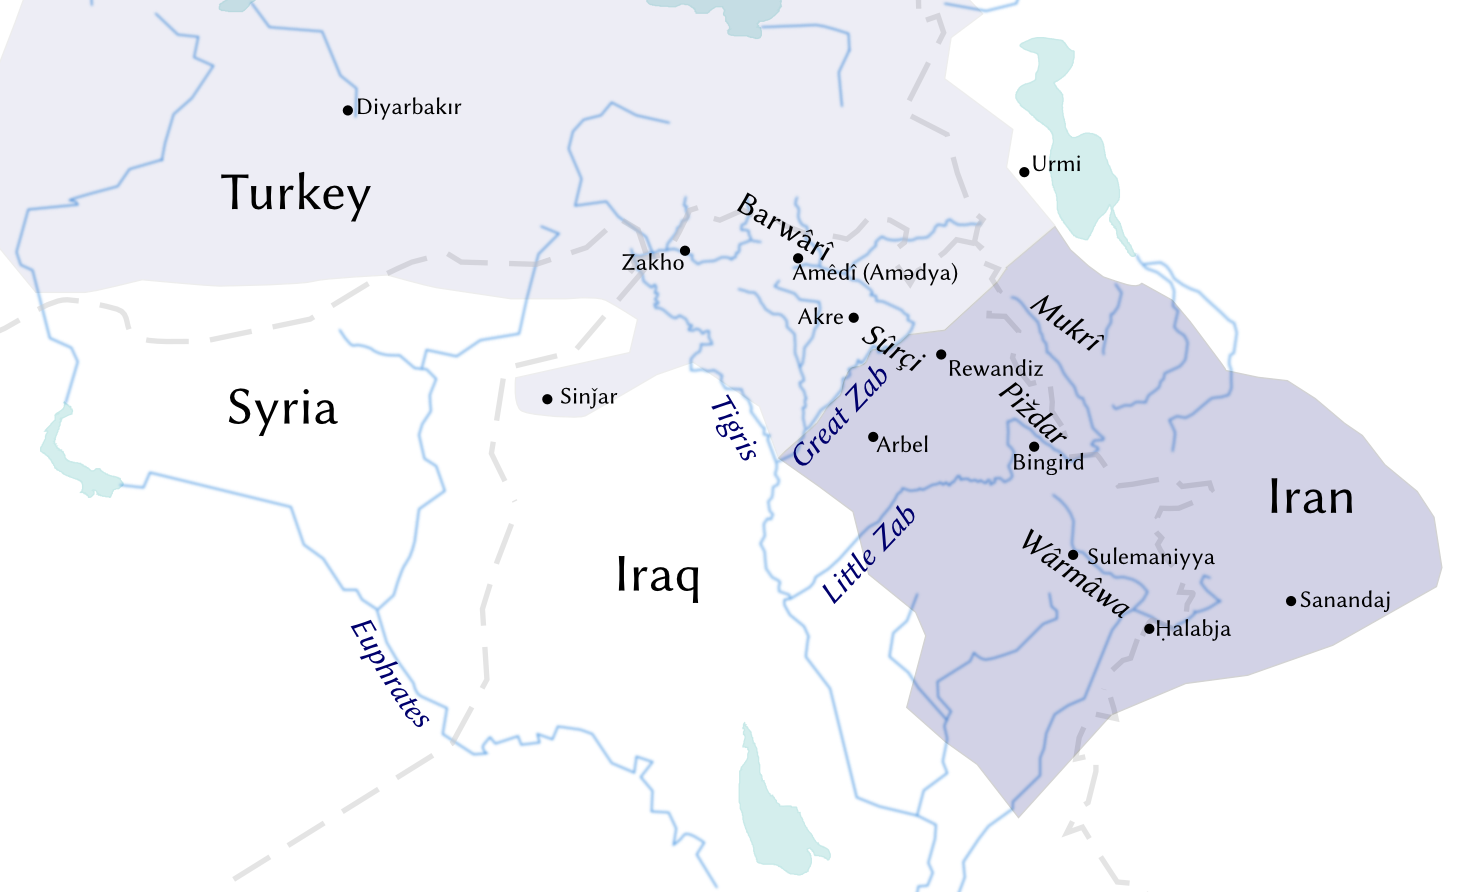
\includegraphics[width=\textwidth]{figures/Kurdishmap.png}
  \caption{Map of surveyed Kurdish dialects and localities. Light grey = Kurmanji dialects; dark grey = Sorani dialects.} \par \label{fg:map_kurdish} 
\end{figure}
  



The chapter is organised as follows: In \sref{ss:Kur_Poss} I treat the possessive pronominal enclitics, present only in \Sor dialects.  The most prominent AC markers in Kurdish are the various \ez* morphemes.  \Sref{ss:three_Ez} gives an overview of the  different forms found in standard Kurmanji and Sorani and motivates the differentiation of three distinct types of \ez* morphemes, discussed in the following sections. \Sref{ss:Kurdish_cst} discusses the Construct \ez* Construction, which can be seen as the Kurdish equivalent of the \ili{NENA} Neo-CSC. The marking of \secns by the \obl* case, present in Kurmanji dialects, is also discussed there.
\Sref{ss:lnk_ez} discusses the Linker \ez* Construction, which can be seen as the Kurdish equivalent of the \ili{NENA} ALC. 
\Sref{ss:Comp_Ez} discusses the usage of the Compounding \ez*, especially productive in \Sor. 
Clausal \secns appear regularly in one of the \ez* constructions, yet they can also appear in some alternative constructions, which are discussed in \sref{ss:Sor_alt_clause}.
The usage of the \isi{juxtaposition} construction, as well as the rare {inverse juxtaposition}\isi{inverse juxtaposition construction}, is presented in \sref{ss:Kur_Juxt}.
Finally, \sref{ss:Kurd_conclusions} concludes this chapter with some general remarks and comparative prospects. 

\largerpage
\section{Possessive pronominal enclitics (X-y.\poss)} \label{ss:Kurd_poss}
\label{ss:Kur_Poss}

Sorani (but not Kurmanji) has a series of unstressed possessive pronominal morphemes. \citet[15]{ThackstonSorani} qualifies them as enclitics, while \citet[76]{MacKenzie} treats them as suffixes. As these elements show promiscuous attachment, attaching indifferently to verbs (as objects; see \cite[37]{ThackstonSorani}), to nouns, and to prepositions, I prefer to analyse them as clitics (see \sref{ss:clitics_affixes}).\footnote{A thorough analysis of their status would require an investigation of their behaviour with verbal hosts, which is beyond the scope of this work. See, in this respect, \citet{SamvelianClitics}, who examines their attachment to verbs and prepositions and concludes, in a final account, that these elements are rather affixes.} 

The pronominal enclitics normally follow the definite or \isi{indefinite suffix}, with the expected meaning: 

\arabex[\Sor]{Noun}{Pronoun}{946}
{كوڕەكەم}
{kuř-eké \cb{}m}
{son-\defi{} \cb\poss.1\sg}
{my son}
{\citep[16]{ThackstonSorani}}

\arabex[\Sor]{Noun}{Pronoun}{834}
{كوڕێكم}
{kúř-êk \cb{}im}
{son-\indef{} \cb\poss.1\sg}
{a son of mine}
{\citep[16]{ThackstonSorani}}

When the noun is left unqualified, this typically yields  a figurative or generic meaning:

\arabex[\Sor]{Noun}{Pronoun}{832}
{كوڕم}
{kúř \cb{}im}
{son \cb\poss.1\sg}
{sonny (form of address for a young boy)}
{\citep[16]{ThackstonSorani}}

The possessive enclitics can appear after compound nominals consisting of a Noun+Adj. combination mediated by the compounding \ez* (see \sref{ss:Comp_Ez}).

\arabex[\Sor]{Compound Noun}{Pronoun}{836}
{كوڕە كۆرپەكەم}
{[kuř-e- korpe]-ké \cb{}m}
{son-\ez{}- newborn-\defi{}  \cb\poss.1\sg}
{my infant son}
{\citep[53]{ThackstonSorani}}

The same \isi{clitic} placement is found when the compounding \ez* is missing due to phonological conditions.  The following \War example can be compared to the \ili{NENA} \JSul \example{1104}:

\acex[\War]
{Compound Noun}{Pronoun}{911}
{[bira-gewr]-ek \cb{}em}
{brother-big-\defi{}  \cb\poss.1\sg{}}
{my elder brother}
{MacKenzie}{81 {[204]}}
 
Finally, the possessive enclitics can follow the focus \isi{enclitic} \foreign{-(î)ş}{also}.

\arabex[\Sor]{Noun}{Pronoun}{1945}
{پارەكەشیان}
{par-eké \cb{}ş \cb{}yan}
{money-\defi{} \cb{}also \cb\poss.3\pl}
{their money too}
{\citep[16]{ThackstonSorani}}

\arabex[\Sor]{Noun}{Pronoun}{835}
{رەفیقەكانیشم}
{refîq-ek-an \cb{}îş \cb{}im}
{friend-\defi-\pl \cb{}also \cb{}\poss.1\sg}
{even my friends}
{\citep[17]{ThackstonSorani}}


Note that in Kurmanji, the lack of possessive pronominal enclitics entails the use of full pronouns which are marked by the \isi{oblique case} (see \example{887}).

\section{The three Ezafe morphemes in Kurdish} \label{ss:three_Ez}

In \sref{ss:ezafe_dispute} I presented briefly the \Per \ez* and the dispute regarding its morphemic status (suffix or \isi{clitic}) and its syntactic attachment (with the \prim or the \secn). Since the \Per \ez* attaches phonologically to the \prim, I concluded, with Samvelian (\citeyear*{SamvelianEzafe, SamvelianHead}),
that the simplest account of the \Per \ez* is to view it as a \isi{phrasal affix} attaching morphologically and syntactically to its \prim, marking the latter as being in \cst*, i.e.\ wanting a complement. 

The situation in Kurdish dialects is somewhat more complex. First, in \Kur, the \ez* morpheme inflects for gender, number, and \isi{definiteness}. More importantly, there are  three distinct types of \ez* markers, differing in their phonological attachment:

\begin{description}

\item[Construct \ez*] Devoid of stress, attaching phonologically to the \prim (-\ez).

\item[Linker \ez*] Can carry stress, and can appear without an immediate \prim (\lnk.\ez).  

\item[Compounding \ez*] Devoid of stress, forming part of a nominal compound \linebreak (-\ez-).

\end{description}

 The various forms of the \ez* in standard Kurmanji and Sorani   are shown in \vref{tb:Ezafe_forms}.

\begin{table}[h!]
\centering
\begin{tabular}{llccc c}
\toprule
			&	& \multicolumn{3}{c}{Kurmanji} & Sorani \\

	&		& \masc 		& \fem 			& \pl		 &		\\
\midrule
\multirow{2}{*}{Construct} & \defi	& \transc{-ê}	& \transc{-a}	& \multirow{2}{*}{\transc{-ên}\footnotemark} & \multirow{2}{*}{\transc{-î}} \\
& \indef& \transc{-î}   & \transc{-e}	&	& \\

Linker & 	& \transc{yê}	& \transc{ya}	& \transc{yên} & \transc{hî} \\

Compounding	&	& \multicolumn{3}{c}{\transc{-e-}}	& \transc{-e-} \\
\bottomrule
\end{tabular}
\caption{The \ez* forms in Standard Kurmanji and Sorani} \label{tb:Ezafe_forms}
\end{table}

\footnotetext{In the Kurmanji dialects overlapping with \ili{NENA}, the regular marking of the plural \ez* is in fact \transc{-êd} or \transc{-êt} \citep[162]{OpenginHaig2014regional}.}

Leaving aside for the moment the compounding \ez*, I note that the (definite) construct \ez* and the Linker \ez* share the same form, except for a weak consonantal onset (\Kur: \phonemic{y-}; \Sor: \phonemic{h-}) marking the latter. In fact, in dialectal data this onset is absent at times. Thus, a natural assumption is to conflate the two sets, arguing these are prosodic variants of each other, one being an \isi{enclitic} and the other (possibly) a \isi{proclitic}. This is the approach taken by \citet[77]{HaigAlignment} and elaborated upon in \citet{HaigLinker}. Yet  as \citet{SamvelianHead} argues (for \Kur), there are distributional reasons for distinguishing the two series: The construct \ez* is in \isi{complementary distribution} with the \isi{oblique case} marking of nouns (present only in \Kur), and thus cannot attach to oblique nouns, while the \lnk* \ez*  is indifferent to the constitution of the \prim.

\acex[\Kur]
{Noun Phrase}{Adjective}{1949}
{[mal-a van jin-an] *-a / ya biçuk}
{house-\ez.\fem{} \dem.\near.\obl.\pl{} woman-\obl.\pl{} *-\ez.\defi.\fem{} / \lnk.\ez.\fem{} small}
{these women’s small house}
{SamvelianHead}{357, examples (47)--(48)}

\largerpage
Since the construct \ez* is in opposition to the \obl* case suffix, \citet[358]{SamvelianHead} analyses it as a suffix (or rather as a \isi{phrasal suffix}), similar to the \Per \ez*, while the \lnk* \ez* is analysed by her as an independent syntactic particle. A similar conclusion is reached by \citet[53]{SchroederAttribution}.
Recall that I used a similar approach to tease apart the \ili{NENA} \cst* suffix \ed and the \isi{proclitic} \lnk* \d (see \sref{ss:d_vs_ed}). 

\citet[79]{Haig2004} objects to this type of analysis (and in particular  to \cite{SchroederAttribution} noting that the \isi{complementary distribution} of the (construct) \ez* and the \isi{oblique case} is not restricted to cases where the \isi{oblique case} is realized by a suffix, but also in the relatively few nouns where the \isi{oblique case} is realized by an internal stem mutation. Thus, one finds \foreigngloss{cem şivan-ê me}{to shepherd-\ez 1\pl.\obl} meaning \transl{to our shepherd} and not \foreigngloss{*cem şivên-ê me}{to shepherd.\obl-\ez 1\pl.\obl}. While I concur with Haig that this demonstrates that the \isi{complementary distribution} of the two markers is not due to \enquote{a low-level constraint on suffix-stacking}, I disagree with his view that the \ez* is not inflectional in nature. In fact, this evidence strengthen the position that the construct \ez* is an inflectional element, as it shows the the \isi{oblique case} marking and the construct \ez* are part of the same abstract paradigm in the Kurmanji linguistic system (a case-cum-state paradigm, as it is), irrespective of the actual realisation of the members of the paradigm. Since the case marking (suffixal or by stem mutation) is clearly inflectional, the same must hold for the \ez*.  

In this study I adhere to Samvelian's analysis, and I shall treat the different types of  \ez* in different sections below. It should be noted, though, that this analysis is especially suitable for \Kur. In \Sor there are no inflectional case endings, and thus the above argument is not applicable.\footnote{In \Sor, on the other hand, nouns can be inflected by the possessive enclitics, discussed in \sref{ss:Kurd_poss}. It would be interesting to see if the construct \ez* is compatible with these enclitics, but unfortunately I have not found data regarding this question. \label{ft:sor_poss_infl}} Yet, as the \Sor construct \ez* appears only after nominal elements (the linker \ez* occurring only without an immediate \prim), it can be seen as a nominal suffix, and therefore I treat  it for simplicity's sake on a par with the \Kur construct \ez*.
 
 
\section{The construct Ezafe construction (X.\textsc{cst} Y)} \label{ss:Kurdish_cst}
\subsection{Introduction}
As explained above, all Kurdish dialects make use of the construct \ez*, a suffix attaching to the \prim phrase, marking it as \cst*. The different varieties of Kurdish differ as to the number of inflectional forms the \ez* exhibits, reflecting various number and gender distinctions. Generally speaking, the number of forms increases as one travels from the south-eastern extremity of Kurdish speaking areas to the north-western extremity. In this perspective, it is useful to take into account also dialects of languages close to Kurdish, such as \ili{Gorani} in the south-east and \ili{Zazaki} in the north-west.\footnote{See \vref{ft:gorani_zazaki} for a discussion of various classifications of these languages.}

In the southern part of my survey of Kurdish dialects, namely in the Sorani dialects, the construct \ez* has a fixed form \transc{-î}\~\transc{-i}\~\transc{-y}.\footnote{\citeauthor{ThackstonSorani} transcribes the \ez* as a lax \transc{i}, separated from its host. Other authors, however, as well as the standard Sorani \ili{Arabic} orthography, treat the \ez* as a tense \transc{î} (in \ili{Arabic} script: \textarabic{ی}), attached to its host. After vowels it is realised as the glide \phonemic{y}. In line with my analysis of the \ez* as a suffix, I transcribe it attached to its host, but I keep the formal variation intact.} Note that the usage of an uninflected \ez* is found also in the \Gawr \ili{Gorani} dialect, spoken in the southern extremity of the Kurdish speaking zone, near the city of Kerend \citep[16]{MahmoudveysiGawraju}; this \ez* has the form \transc{-e}\~\transc{-y}, akin to the uninflected \Per \ez* \transc{-(y)e}.

\arabex[\Sor]{Noun}{Noun}{821}
{كتاویەكانی قوتابخانەیەك}
{ktawî-ek-an-i qutabkhane-yêk}
{student-\defi-\pl-\ez{} school-\indef}
{the students of a school}
{\citep[10]{ThackstonSorani}}

\acex[\KSul]{Noun}{Noun}{897}
{ser-î binîâdem}
{head-\ez{} man}
{men's heads}
{MacKenzie}{63 {[49]}}

As \example{821} shows, the \prim and \secn can be independently marked as definite or indefinite. If they are left unmarked, as in \example{897}, the AC may be interpreted generically.

The same construction can be used with a full pronominal \secn, as an alternative to the usage of the possessive enclitics (see \sref{ss:Kur_Poss}), for \enquote{special emphasis} \citep[179]{AbdullaMcCarus}.

\acex[\KSul]{Noun}{Pronoun}{945}
{nàv-i mín}
{name-\ez{} 1\sg}
{\textit{my} name}
{AbdullaMcCarus}{179}


As one travels northwards, roughly to the \emph{Inter-Zab}\il{Inter-Zab dialects} region (between the Little Zab and the Great Zab rivers), more variation appears. In some Sorani dialects (namely, \Muk and \Rdz) the \ez* may appear as \transc{-(y)e} following a vowel \citep[62]{MacKenzie}. 

\acex[\Rdz]{Noun}{Pronoun}{882}
{kursî-(y)e min}
	{seat-\ez{} 1\sg}
{my seat}
{MacKenzie}{62 {[484]}}

 This is purely a phonological variant of the \ez*. More interesting  is that some north-eastern Sorani dialects (\Bin, \Piz and \Muk) exhibit an optional \ez* form, \transc{-ê}, reserved for \fem* \sg* nouns \citep[61]{MacKenzie}. This is shown by the following example:
 
 \acex[\Muk]{Noun}{Proper Noun}{877}
 {xuşk-ê Mîr Zêndîn}
 {sister-\ez.\fem{} M. Z.}
 {Mir Zendin's sister}
 {MacKenzie}{61 {[30]}}
 
  In the same dialects, whenever the \prim has plural sense but no formal marking of this (as an unmarked noun can be interpreted singularly or plurally), an extra particle \transc{de} may follow the \ez*.\footnote{It is a curious fact that this \pl* \ez* marker has a  similar form to the Aramaic \lnk* \d. Yet, as the Aramaic \lnk* is not related in any way to marking of plurality, this is very likely a pure coincidence.}
  
  \acex[\Bin]{Noun}{Noun}{883}
  {pyaw-î de paşe}
  {man-\ez{} \pl{} king}
  {the king's men}
  {MacKenzie}{62 {[319]}}
  
  The same marker is used whenever the \prim consists of a conjunction of two singular nouns. In such cases, the \ez* is attached phrase-finally. 
  
   \acex[\Bin]{Conjoined nouns}{Pronoun}{887}
   {[dak û bab]-î de to}
   {mother and father-\ez{} \pl{} 2\sg}
   {thy mother and father}
   {MacKenzie}{62 {[349]}}
 
  Among the Kurmanji dialects, a distinction between the two genders is obligatory, as is shown in \vref{tb:Ezafe_forms}. Most dialects also have a separate \pl* \ez*, though sometimes it is assimilated with the \masc*  \sg* form. The usage of the \pl* form as well as the \fem* form is shown in the following example, which shows also the possibility to embed the \ez* construction:
  
  \acex[\Kur]{Noun}{Noun Phrase}{711}
  {kitêb-ên [keç-a mirov]}
  {book-\ez.\defi.\pl{} girl-\ez.\fem{} man}
	  {the man's daughter's books}
  {ThackstonKurmanji}{13}
  
  In some older literary texts, one finds the same plural particle as in the Sorani dialects mentioned above (see \examples{883}{887}). Such is the case, for instance, in the poetry of the Kurdish poet Malaye Jaziri of Bohtan (1570-1640)\footnote{These years are given by \citet[176]{IzadyKurds}, who writes the poet's name as \textit{Mullâ-i Jaziri}.}:
  
  \arabex[\Kur]{Noun}{Adjective}{891}
  {چشمین دِ سِيَه}
  {çeşm-ên di siyeh}
  {eye-\ez.\defi.\pl{} \pl{} black}
  {black eyes}
  {(Malaye Jaziri, \textit{Diwân}, ed.\ \cite[217]{Hartmann}; \cite[159, fn.\ 2]{MacKenzie})}
  
The \Kur \ez*, just like the \Sor \ez* shown in \example{887}, attaches phrase-finally to the \prim, and has scope over the whole \prim phrase. According to the description of \citet{BedirKhan}, the inflectional features carried by the \Kur \ez* suffix are, however, only dependent on the noun to which it directly attaches (this is also the case in \example{752}, cited from \citeauthor{ThackstonKurmanji}):\footnote{One reviewer noted that this is not a strict rule but subject to dialectal variation, bringing the following example from the Zakho dialect: \foreigngloss{kič u kur-ēt min}{daughter and son-\ez.\pl{} 1\sg.\obl} meaning \transl{my daughter and son}. Note that the plural \ez* is used due to the plurality of the NP but attaches to a singular noun.} 



 \acex[\Kur]{Conjoined nouns}{Pronoun}{950}
 {[dê û bav]-ê min}
 {mother and father-\ez.\defi.\masc{} 1\sg.\obl}
 {my mother and father}
 {BedirKhan}{2}
 
 \acex[\Kur]{Conjoined nouns}{Pronoun}{951}
  {[ker, hesp û mehîn]-a min}
  {donkey, horse and mare-\ez.\defi.\fem{} 1\sg.\obl{}}
  {my donkey, horse and mare}
  {BedirKhan}{2}
 
 
 This behaviour indicates that the \Kur \ez* should be analysed as a \isi{phrasal suffix}: while morphologically it is tied to the nominal inflectional system and thus shows inflectional features of the noun it attaches to, syntactically it marks the entire NP as being in \cst* and  has thus wide syntactic scope (see \sref{ss:clitics_affixes} and in particular \vref{tb:continuum}).
 
Likewise, if the last noun of the \prim has a plural sense by itself, it will receive the \pl* \ez* suffix. In such cases the \pl* sense may be inferred pragmatically also for the other conjunct nouns of the \prim, as in the following example:\footnote{Note that a \Kur noun without \ez* or \obl* case marking is unmarked for number, and may be interpreted either as \pl* or as \sg* according to the context.}
  
\acex[\Kur]{Conjoined nouns}{Noun}{724}
{[şexsiyet û rewşenbîr]-ên kurd-an}
{personality(\fem) and intellectual-\ez.\defi.\pl{} Kurdish-\obl.\pl{}}
{personalities and intellectuals of the Kurds}
{ThackstonKurmanji}{15}


 
  \citeauthor{BedirKhan}  notes that this pattern  only arises with the conjunction \foreign{û}{and}. When the \prim NP consists of nouns joined using the disjunctive conjunction \foreign{(y)an}{or}, each element must belong to a separate AC.   
 
 \acex[\Kur]{Disjoined Nouns}{Pronoun}{952}
 {hesp-ê min an mehîn-a min}
 {horse-\ez.\defi.\masc{} 1\sg.\obl{} or mare-\ez.\defi.\fem{} 1\sg.\obl}
 {my horse or my mare}
 {BedirKhan}{2}
  
  
  The \Kur \ez* inflects also according to the \isi{definiteness} of the noun.  Yet, in contrast to its number and gender inflection, the (in)\isi{definiteness} feature is  not carried by the \ez* suffix, but rather it co-varies  with the presence of a singular \isi{indefinite suffix} \transc{-êk} \citep[158-160]{MacKenzie} or a plural \isi{indefinite suffix} \transc{-in} \citep[78]{BedirKhanLescot}. 
  
  \acex[\Kur]{Noun}{Noun}{708}
  {hejmár-ek-e kovár-ê}
  {issue(\fem)-\indef-\ez.\indef.\fem{} journal-\obl.\fem{}}
  {an issue of that journal}
  {ThackstonKurmanji}{12}\antipar
  
  
   \newpage
  \acex[\Kur]{Noun}{Noun}{949}
  {mehîn-in-e keçk-ê}
  {mare-\pl.\indef-\ez.\indef.\pl{} girl-\obl.\fem}
  {some mares of the girl}
  {BedirKhanLescot}{306}\antipar
    
  
  Since these allo-forms depend on the explicit presence of an \isi{indefinite suffix}, \citet[355-357]{SamvelianHead} rejects the notion of the \concept{indefinite ezafe}, analysing these forms instead as being conditioned by their post-affixal position. She shows that an indefinite \pl* noun not marked by the suffix \transc{-in} takes the normal form of the \ez*  \transc{-ên}:
  
  \acex[\Diar]
  {Noun}{Adjective}{1950}
  {pênc kur-ên ganc}
  {five boy-\ez.\pl{} young}
  {five young boys}
  {SamvelianHead}{356, example (45)}
  
  This pattern, however, could equally well be analysed as a neutralisation of the \isi{definiteness} feature of the \pl* \ez* (as presented in \vref{tb:Ezafe_forms}). Such a neutralisation may be motivated by the fact that the explicit marking of \pl* indefinite nouns by means of the   suffix \transc{-in} is quite rare (judging by the sources consulted), and that the indefinite \pl* \ez* \transc{-e} is  identical in form to the indefinite \fem* form, as is shown in \examples{708}{949}.
  
  \citet[356]{SamvelianHead} substantiates further her claim by citing   \citet[158]{MacKenzie}, who mentions that in \Sur dialect, the indefinite form (termed by him \concept{secondary ezafe}), follows \enquote{apparently} also the \isi{definite suffix} \transc{-eke}:
  
  \acex[\Sur]
  {Noun}{Adjective}{1951}
  {mirow-eke-y xwarê}
  {man-\defi-\ez.\masc{} lower}
  {the lower man}
  {MacKenzie}{160 {[517]}}
   
  Yet  most \Kur dialects lack the \isi{definite suffix} \transc{-eke}, which is more typical of \Sor dialects. Thus, leaving aside such exceptional examples (whose status seems to be questioned by \citeauthor{MacKenzie} himself), it seems justifiable to regard the \sg* \ez* forms \transc{-î} (\masc) and \transc{-e} (\fem) as allomorphic forms signalling indefiniteness of the \prim noun.\footnote{Note, however, that \transc{-î} is also used in some contexts where no indefiniteness is implied, such as with \isi{adverbial} \prims (see \sref{ss:cst_ez_adv_prim}).}
  
  


The same cline of explicitness can also be found regarding the marking of the \secn by  \isi{oblique case}. This is treated in \sref{ss:Kurd_obl}.




\subsection{Oblique marking of \secns} \label{ss:Kurd_obl}


\Kur exhibits a bipartite case system, opposing the unmarked direct case with a marked \isi{oblique case}, visible on nouns and pronouns. On nouns, the \isi{oblique case} is normally marked by suffixes, which express moreover the gender and number features of the host noun. These suffixes are shown in \vref{tb:Obl_forms}.

\begin{table}[h!]
\centering
\begin{tabular}{l ccc}
\toprule
			&	\masc & \fem & \pl \\
\midrule
Direct		& \multicolumn{3}{c}{\zero} \\
Oblique		& \zero\ / \transc{-î}	& \transc{-(y)ê}	& \transc{-(y)an} \\
\bottomrule
\end{tabular}
\caption{Kurmanji case endings} \label{tb:Obl_forms}
\end{table}

A particularity of the \masc* \sg* oblique suffix is that it appears only if the host noun is qualified by a determiner.\footnote{This is the rule in Standard Kurmanji. Yet in the Kurmanji dialects overlapping with the \ili{NENA} speaking zone, there is a consistent suffix-marking of the oblique. See the discussion of \citet[162]{OpenginHaig2014regional} and \citet{HaigOpengin2017structure} regarding the \enquote{Southeastern} Kurmanji dialect group.} 
Yet a few masculine nouns show the \isi{oblique case} by internal mutation, replacing an ultimate \phonemic{a} vowel by an \phonemic{ê} vowel \parencites[9]{ThackstonKurmanji}[73]{Haig2004}. For example, \foreign{bajar}{city} is \transc{bajêr} in the \isi{oblique case} (see \example{955}).

The \isi{oblique case} marks the dependents of both the \isi{attributive relation} and the \isi{completive relation} (see \sref{ss:threeRel}). It subsumes thus both the \isi{genitive case} and the accusative case (and in the \Kur context, also the ergative case). Note, moreover, that similarly to the \ez* the oblique suffixes can have phrasal scope, appearing on the final noun of conjoined nouns, and only optionally on the preceding nouns.\footnote{In this respect it is also somewhat different to the \ez*, as the \ez* can only appear on the last conjoined noun, since it must be followed immediately by the \secn.} This is demonstrated by the following example, in which the \obl* case takes the accusative role.

\acex[\Kur]
{Verb}{Conjoined Nouns (objects)}{Sam_Obl}
{[jin-\opt{ê} u kur-î] di-bîn-im}
{woman-\opt{\obl.\fem} and boy-\obl.\masc{} \ind-see-1\sg}
{I see the woman and the boy}
{SamvelianHead}{354, example (41)}\antipar\antipar

\newpage 
In this study, I am interested mainly in the \gen* function of the \obl* case, namely the marking of AC \secns. This is shown in the following example (as for the oblique demonstrative, see \vref{tb:kur_dem}):

\acex[\Kur]{Noun}{Noun}{706}
{miróv-ek-î  [w-î weláṭ-î]}
{man-\indef-\ez.\indef.\masc{} \dem.\far-\obl.\masc{} country-\obl.\masc}
{a man of that country}
{ThackstonKurmanji}{12}

For examples of \fem* and \pl* oblique endings, see \examples{724}{708}.

It is important to note that the \ez* suffix and the \obl* marking (suffixal or by stem mutation) are morphologically in \isi{complementary distribution}, although notionally they mark independent features, the \ez* being related to the state category.\footnote{\textit{Pace} \citet[7]{ThackstonKurmanji} who speaks of construct \enquote{case}. In the \ili{Zazaki} language, related to Kurmanji, a noun can be marked both for \isi{oblique case} and the \isi{construct state} by means of a specially inflected \ez* \parencites[43]{Todd}[and see further][]{LarsonYamakido}{SamvelianHead}{PlankSuffixaufnahme2012}. See also the discussion at the end of \sref{ss:three_Ez}.} Thus, a \secn noun itself acting as \prim is only marked by the \ez*. An \obl* suffix, if present at all, can only be marked in such cases at the end of the \secn phrase:

\acex[\Kur]
{Circumposition}{Noun Phrase}{713}
{di [gund-ên kurd-ên Kurdistan-a Tirkiye-yê] de}
{in village-\ez.\pl{} Kurd-\ez.\pl{} Kurdistan-\ez.\fem{} Turkey-\obl.\fem{} in}
{in the villages of the Kurds of Turkey's Kurdistan}
{ThackstonKurmanji}{13}

Kurmanji dialects also have  a series of full oblique pronouns, which can be used as \secns. These are the functional equivalents of the Sorani possessive pronominal enclitics, described in \sref{ss:Kurd_poss}. For example, the direct pronoun \foreign{ez}{I} has the oblique form \transc{min} (see its occurrence also in \examples{950}{951}):

\acex[\Kur]{Noun}{Pronoun}{743}
{kitêb-a min}
{book-\ez.\defi.\fem{} 1\sg.\obl}
{my book}
{ThackstonKurmanji}{18}

\newpage 
In contrast to nouns, an oblique pronoun can further be marked by the \ez* suffix:\footnote{Yet  this may in fact be an instance of the linker \ez* discussed in \sref{ss:lnk_ez} phonologically encliticized to the \prim, as it does not necessarily show the inflectional features of its host pronoun, as would be expected from the construct \ez*. Thus, in the following example, the \ez* suffix \transc{-a} shows agreement with the \prim \foreign{mal}{house} rather than with the pronoun \transc{min} (given that the speaker is a man):

\acexfn[\Kur]
{Pronoun}{Noun}{1954}
{mal-a [bira-yê min]-a biçuk}
{house.\ez.\fem{} brother-\ez.\masc{} 1.\sg.\obl-\ez.\fem{} small}
{my brother's small house}
{SamvelianHead}{354, example (40)}
 
See \example{768} for a clear case of the \lnk* \ez* following \transc{min}.
 }

\acex[\Kur]
{Pronoun}{Noun}{1953}
{min-ê bêçâra bibîna}
{1.\sg.\obl-\ez.\masc{} poor look.\imp}
{Look at me, poor thing}
{SamvelianHead}{353, example (39)}

In contrast to Kurmanji, the south-eastern Sorani dialects (and notably the dialect of Sulemaniyya, which is the basis for standard Sorani) have no case system at all. The Sorani dialects to the north, however, show an oblique suffix for singular \secns:\footnote{The \pl* is marked by a case-neutral suffix \transc{-ân} \citep[58]{MacKenzie}.}

\acex[\Bin]{Noun}{Noun}{898}
{lep-î dest-î}
{palm-\ez{} hand-\obl.\masc{}}
{palm of the hand}
{MacKenzie}{59}

\acex[\Bin]{Noun}{Noun}{899}
{zîn-î maîn-ê}
{saddle-\ez{} mare-\obl.\fem{}}
{saddle of the mare}
{MacKenzie}{59}

\newpage 
\subsection{Adjectival \secns}


The \ez* construction is used also with adjectival \secns. In \Kur, adjectives differ from nouns by the fact that they never inflect and thus do not take an \obl* suffix \citep[163]{MacKenzie}.\footnote{Note, however, that the denominal adjective derivational suffix \transc{-î} is conspicuously similar to the \masc* \sg* oblique ending, making an historical connection between the two possible. This recalls the situation in the \ili{Semitic} domain, where  a formal similarity can be observed between the \Arab adjectival ending \transc{-iyy} and the \gen* case \transc{-i}. The usage of the oblique suffixes as derivational suffixes is much clearer in the case of the \Kur \isi{ordinals}; see \ref{ss:kurd_ez_ord}.}


\acex[\Kur]{Noun}{Adjective}{715}
{mirov-ek-î mezin}
{man-\indef-\ez.\indef.\masc{} big}
{a big man}
{ThackstonKurmanji}{14}

\acex[\KSul]{Noun}{Adjective}{893}
{tûtik-êk-î piçkołe}
{dog-\indef-\ez{} small}
{a little dog}
{MacKenzie}{63 {[69]}}


As the above examples show, the \prim can be determined by the \isi{indefinite suffix} in both \Kur and \Sor. In Kurmanji dialects, a definite sense is obtained by using the definite \ez*:

\acex[\Kur]{Noun}{Adjective}{714}
{mirov-ê mezin}
{man-\ez.\defi.\masc{} big}
{the big man}
{ThackstonKurmanji}{14}

\largerpage
In Sorani, however, a \prim noun followed by an adjective is not normally combined with the \isi{definite suffix} \transc{-eke}. Instead, whenever a definite \prim is needed, the compounding \ez* is used (see \sref{ss:Comp_Ez}). It seems, however, that the construct \ez* construction is compatible with a definite \prim, if the adjective has a descriptive, rather than restrictive, sense \citep[see][12, fn.~1]{ThackstonSorani}. 

\arabex[\Sor]
{Noun}{Adjective}{831}
{دەرسەكانی سەخت}
{ders-ek-an-i sext}
{lesson-\defi-\pl-\ez{} hard}
{the lessons, which are hard}
{\citep[12]{ThackstonSorani}}\antipar 

\newpage 

Whenever a \prim is modified by more than one adjective, several alternative patterns are available. The adjectives may be conjoined to form one \secn phrase:

\acex[\KSul]{Noun}{Conjoined Adjectives}{903}
{minał-êk-î [pîs û poxił]}
{child-\indef-\ez{} dirty and filthy}
{a filthy, dirty child}
{MacKenzie}{63}

\acex[\Kur]{Noun}{Conjoined Adjectives}{947}
{keç-ên [por-zer û çav-şîn û kesk]}
{woman-\ez.\pl{} hair-yellow and eye-blue and green}
{blonde and blue- and green- eyed women}
{ThackstonKurmanji}{98}

Another possibility is to chain the subsequent adjectives by \ez* suffixes, as the following Sorani examples show. In such cases one might expect the two adjectives to have  different scopes (the first qualifying the \prim noun only, while the second qualifies the N+Adj. combination), yet this is not apparent from the translations:

\arabex[\Sor]{Noun}{Adjectives}{852}
{شارێكی گەورەی تازە}
{[shar-êk-î gewre]-y taze}
{city-\indef-\ez{} big-\ez{} modern}
{a big modern city (\textit{une grande ville moderne})}
{\citep[60]{BlauSorani}}

\acex[\KSul]{Noun}{Adjectives}{904}
{[kiç-êk-î jwan]-î çwar-de \cb{}sał}
{girl-\indef-\ez{} pretty-\ez{} four-teen \cb{}year}
{a beautiful, fourteen-year-old girl}
{MacKenzie}{63}

\largerpage
This latter possibility seems to be unavailable for Kurmanji dialects, which instead make use of the \lnk* \ez* construction  in such cases (see \sref{ss:lnk_ez}).\footnote{See however the rare usage of the \Kur \lnk* \ez* \transc{î} in \examples{742}{955}, which, notwithstanding the difference in analysis, is very similar formally to the construct \ez* in  the  above cited \Sor examples.}  
This is correlated with the fact that the Kurmanji \ez* is a nominal inflectional suffix, incompatible with adjectives, which never inflect. The \Sor \ez*, on the other hand, does not \emph{prima facie} form part of an inflectional system, and in this respect shows \isi{clitic} behaviour (but see \vref{ft:sor_poss_infl}). 



\subsection{Adjectival \prims}

In Sorani, one finds that adjectives extended by nominal complements get the \ez* suffix: 

\acex[\Muk]{Adjective}{Noun}{914}
{xerîk-î bezm-î (de-bû-n)}
{busy-\ez{} feasting-\obl(?) \ind-be-\pl}
{(They would be) engaged in feasting.}
{MacKenzie}{65 {[3\textsuperscript{25}]}}

\acex[\KSul]{Adjective}{Noun}{915}
{tûş-î em derd-e}
{afflicted-\ez{} \dem.\near{} trouble-\defi}
{afflicted by this trouble}
{MacKenzie}{65 {[67]}}

Note that \example{914} is very similar to the \ili{NENA} \JSan \example{98}. 

In \Kur, such examples are not expected to be found, as adjectives are normally not marked by the construct \ez* (see discussion at the end of the previous section). Yet  \citet[343]{SamvelianHead} affirms the existence of this construction:

\acex[\Kur]
{Adjective}{Noun}{1946}
{Azâd âşiq-ê Narmîn-ê ya}
{A. in\_love-\ez.\masc{} N.-\obl.\fem{} \cop.3\masc}
{Azad is in love with Narmin.}
{SamvelianHead}{343, example (15)}

Note, however, that \citet[197]{ThackstonKurmanji} lists this construction only in combination with the verb \transl{to be} (\transc{ʿaşiq-e ... bûn}), rendering it possibly a fixed collocation. 

\subsection{Ordinal \secns} \label{ss:kurd_ez_ord}
\largerpage[1.5]
Ordinals follow the \ez* as regular \secns. In standard \Kur they are derived from the cardinal numerals by a fixed \obl* \pl* suffix \transc{-yan}, except for the \isi{numeral} \transl{first}, which has a special form \transc{ewel(î)} in which one can recognize the \masc* \sg* \obl* ending \transc{-î}. Alternatively, \isi{ordinals} (including \transl{first}) may be derived by taking the suffix \transc{-ê(m(în))} of \Per origin \citep[25]{ThackstonKurmanji}.\footnote{According to \citet[170, \S 274.(a)]{MacKenzie}, the \Kur dialects form \isi{ordinals} by the  suffix \transc{-ê} (see \example{808}), which he relates to the identically formed superlative suffix \citep[164, \S 268.(b)]{MacKenzie}. In this case, it is the equivalent of \Sor suffix \transc{-în}, serving as a superlative \citep[68, \S 190.(b)]{MacKenzie}; see \vref{ft:superlative_ordinals}.\label{ft:superlative_e}}

\acex[\Kur]{Noun}{Ordinal}{750}
{roj-a sisi-yan}
{day-\ez.\defi.\fem{} three-\obl.\pl}
{(on the) third day}
{ThackstonKurmanji}{25}

\acex[\Kur]
{Noun}{Ordinal}{1952}
{car-a yeḳ-em}
{time-\ez.\defi.\fem{} one-\ord}
{the first time}
{ThackstonKurmanji}{25}

 In Sorani, \isi{ordinals} are similarly derived from the cardinal numerals by means of the suffix \transc{-(h)em} \citep[72--73]{MacKenzie}.

\acex[\KSul]{Noun}{Ordinal}{924}
{řêga-y sê-hem}
{third-\ez{} three-\ord}
{the third road}
{MacKenzie}{72 {[47]}}

 Alternatively, \Sor uses a longer ordinal suffix \transc{-(h)emîn} (borrowed in  \ili{NENA} \JUrm  and \JSan; see \example{130} and \example{281}). Yet when  \isi{ordinals} are derived by the full suffix \transc{-emîn}, they are not used in the \ez* construction, but rather in the \isi{inverse \isi{juxtaposition} construction} (see \example{1915}).


\subsection{Adverbial \secns} \label{ss:cst_ez_adv_secn}

In Kurmanji, prepositional phrases can regularly occur as \secns following the construct \ez*:\footnote{The usage of \cst* marker followed by \PP s is known also in the Aramaic domain. For Syriac, see \examples{1116}{1151}; for \JZax, see \examples{378}{377}; \JUrm: \example{148}.}

\acex[\Sor]{Noun}{\PP}{722}
{rojname-yek-e [bi kurdî]}
{newspaper-\indef-\ez.\indef.\fem{} in Kurdish}
{a newspaper in Kurdish}
{ThackstonKurmanji}{14}

In Sorani, this construction is not mentioned in the sources consulted, except by  \citet[346]{SamvelianHead}, who lists it as a regular construction:

\acex[\Sor]
{Noun}{\PP}{1948}
{xânu-y [la sar şâx]}
{house-\ez{} at head mountain}
{the house on the mountain}
{SamvelianHead}{346, example (19)}



\subsection{Adverbial  \prims} \label{ss:cst_ez_adv_prim}

Some nominals and adverbs can be used as prepositions. 
In \Kur, they may be marked by a frozen uninflected \ez* \transc{-î} termed by \citet[200]{MacKenzie} the \concept{generic ezafe}. Note, moreover, that complements of prepositions in \Kur are regularly marked by the \obl* case. 



\acex[\Ak]{Adverbial Noun}{Noun}{784}
{nêzîk-î ḥakim-i}
{near-\ez{} judge-\obl.\masc}
{near the judge}
{MacKenzie}{161 {[602]}}


See also \example{752} for the usage of the circumposition \foreigngloss{ji ali-yê ... ve}{from side-\ez.\masc\ ... from} introducing a passive agent. 

In \Sor, an \isi{adverbial} noun is similarly sometimes marked by the \ez* (but see \example{1955}):

\acex[\KSul]
{Adverbial Noun}{Pronoun}{943}
{la dwâ-y min}
{at last-\ez{} 1\sg}
{after me}
{AbdullaMcCarus}{75}

\subsection{Verbal nouns as \prims} \label{ss:cst_ez_verbal}

Verbal nouns, be they infinitives or nouns participating in complex predication (CP nouns), can be complemented by an argument following the construct \ez*.\footnote{Compare this to the situation in Aramaic; \Syr \isi{participles}: \examples{1151}{1117}; \JZax infinitives: \sref{ss:JZax_inf_head}; \Qar infinitives: \sref{ss:Qar_CSC_inf} \JUrm \isi{participles}: \example{122}; \JSan CP noun: \example{49}.} Note that \Kur infinitives have feminine gender and are hence marked by \fem\ \ez* \citep[32]{ThackstonKurmanji}. 

\acex[\Kur]{Infinitive}{Pronoun (subject)}{768part}
{çûyîn-a min}
{go.\inf-\ez.\defi.\fem{} 1\sg.\obl{}}
{my going}
{}{(\cite[33]{ThackstonKurmanji}; see \example{768} for a fuller context)}

\arabex[\Sor]
{Infinitive}{Noun Phrase (object)}{828}
{بۆ توانینی ئەم دیاری جێگای میر گەورەیە}
{bo twanîn-i [em dyarî kirdin-i [cêga-i Mîr Gewre] \cb{}yé]}
{for be\_able.\inf{}-\ez{} \dem.\near{} clarification do.\inf{}-\ez{} position-ez{} M. G. \cb{}\defi  }
{in order to enable this clarification of Mir Gawra’s position}
{\citep[12]{ThackstonSorani}}




\acex[\KSul]{CP Noun}{Noun (object)}{913}
{swar-î řexş bû}
{horseman-\ez{} steed was}
{He mounted his steed.}
{MacKenzie}{65 {[66]}}

The argument occupying the \secn can also be an indirect object. Such is the case in the following example, in which the direct object \transc{vê kaġez-ê} is governed directly by the verb, while the indirect object is governed by a CP noun. 

\acex[\Ak]{CP Noun}{Noun (indirect object)}{788}
{vê kaġez-ê teslîm-î [filan wezîr-î] bi-k-e}
{\dem.\near.\obl{} letter-\obl.\fem{} giving-\ez{} such\_and\_such vizier-\obl.\masc{} \subj-do-2\sg}
{Give this letter to such and such a vizier!}
{}{(\cite[161]{MacKenzie}; \cite[274]{MacKenzieTexts} {[603]})}















\subsection{Clausal \secns and the use of the relativizer} \label{ss:cst_ez_clausal}

Relative clauses, or, in other words, clausal \secns, make use of the \ez* construction as well, with the addition that normally a special particle, a \isi{relativizer}, introduces the clause. Thus, the \ez* signals that the \prim is to be modified, while the \rel* marks the clause as a \secn.\footnote{In Sorani, \citeauthor{ThackstonSorani} distinguishes between the \ez* introducing a \isi{relative clause}, being a tense \transc{-î}, and the regular \ez*, being a lax \transc{i}. As we have seen, other authors transcribe the regular \ez* as a tense \transc{î} as well, rendering this distinction apparently artificial.} In Sorani, the \rel* is \transc{\textarabic{كە} ke} while in Kurmanji it is \transc{ḳu}.\footnote{\citet{HaigLinker} treats  \transc{ḳu} as a \isi{complementizer}, while \citet{ThackstonKurmanji} regards it as a relative pronoun. Since the current study deals here only with cases where \transc{ḳu} is followed by a \isi{relative clause}, I will treat it as a \isi{relativizer} (glossed \rel), without committing to its general status. Recall that the under-dot of \phonemic{ḳ} signals an unaspirated and/or pharyngealized consonant, a phonemic distinction that is normally not marked in standard \Kur orthography (\citeauthor[4]{ThackstonKurmanji} marks it with an underscore and describes it as an unaspirated stop accompanied by pharyngealization \phonetic[kˁ].} 

\arabex[\Sor]{Noun}{Clause}{837}
{سەری كوڕەكەی كە نوستبوو}
{ser-i [kuř-eké-î ke nustibû]}
{head-\ez{} boy-\defi-\ez{} \rel{} slept.3\masc}
{the head of the boy, who has fallen asleep}
{\citep[73]{ThackstonSorani}}

\arabex[\Sor]{Noun}{Clause}{872}
{ئەو كراسەی كە تۆ كـڕیوتە}
{ew kiras-e-y ke [to kiřî-w-t-e] (zor drêj \cb{}e)}
{\dem.\far{} dress-\defi-\ez{} \rel{} 2\sg{} bought-\prf-2\sg-\cop.3\sg{} very long \cb{}\cop.3\sg}
{The dress that you bought (is very long).}
{\citep[156]{BlauSorani}}

\acex[\Kur]{Noun}{Clause}{753}
{wî ziman-ê ḳu [li ber mirinê ye]}
{\dem.\far.\obl{} language-\ez.\defi.\masc{} \rel{} at fore die.\inf.\obl.\fem{} \cop.3\sg}
{this language, which is on the verge of dying}
{ThackstonKurmanji}{75}

\acex[\Kur]{Noun Phrase}{Clause}{752}
{[ew alfabe û rêziman]-a ḳu [ji ali-yê Celadet Bedir-Xan ve haṭiye danîn]}
{\dem.\far{} alphabet and grammar-\ez.\defi.\fem{} \rel{} from side-\ez.\masc{} C. B.-X. from \pass.\prf{} put\_down.\inf}
{the alphabet and grammar that were established by Djeladet Bedir Khan}
{ThackstonKurmanji}{75}\antipar\antipar 
\newpage 

The \rel* can be omitted, especially (but not exclusively) when the \prim refers to the object of the subordinated verb, according to  \textcites[73]{ThackstonSorani}[77]{ThackstonKurmanji}. \citet[157]{BlauSorani}, however, relates its omission to the definite marking of the \prim.


\arabex[\Sor]{Noun Phrase}{Clause}{843}
{ئەو دوو فرمێسكە گەورەیەی ئەیانەوێ  بكەونە خوارێ}
{[ew dû firmêsk-e- gewre-yé]-î [e-yan-ewê bi-kew-in-à xwarè]}
{\dem.\far{} two tear-\ez- big-\definite{}-\ez{} \ind-3\pl-want \subj-fall-3\pl{}-\dir{} down}
{those two large tears, which were about to dribble down}
{\citep[75]{ThackstonSorani}}

\acex[\Kur]{Noun}{Clause}{759}
{ṭişṭ-ên [min nivisîbûn]}
{thing-\ez.\defi.\pl{} 1\sg.\obl{} written}
{the things I had written}
{ThackstonKurmanji}{77}

\acex[\Sor]{Pronoun}{Clause}{932}
{ewe-y to dîwite}
{\dem-\ez{} 2\sg{} seen}
{that which thou hast seen}
{MacKenzie}{133}

See also the the discussion of \citet[203--204]{MacKenzie} who presents various examples of \Kur relative clauses, with or without the \rel*.


\section{The linker Ezafe construction (X \textsc{lnk} Y)} \label{ss:lnk_ez}
\subsection{Introduction}
In Kurmanji dialects alone, an independent (i.e. not suffixed) \ez* may appear between a \prim and a \secn.
This happens most frequently whenever the \prim is a noun phrase, rather than a simple noun. A nominal \secn is, as expected, marked with the \obl* case (which is however \zero\ for undetermined \masc* \sg* nouns), while adjectives  remain  uninflected.

The linker \ez* is very similar in form to the definite suffixed \ez*, except that it is usually preceded by the segment \transc{y-} (which can, however, be elided in certain dialects and certain phonological environments). Thus, as discussed in \sref{ss:three_Ez}, it is possible to consider  the two forms as essentially one and the same morpheme, which cliticizes to the \prim whenever it follows it immediately. Nonetheless, following the argumentation of \citet{SamvelianHead}, I distinguish between the two cases as manifesting different constructions. Moreover, in accordance with this study's framework the independent \ez* has all the characteristics of a pronominal \lnk*, as it can represent alone the \prim (see \sref{ss:lnk_zero_prim}), sharing with it, moreover, the number and gender features.

The \lnk* \ez* is used most often when the \prim consists of a noun phrase, ending with an adjective\footnote{Note that in this respect the \Kur construct \ez* is different from the \Per \ez*, as the latter can appear following adjectives (see \example{1917}). In fact, the \Per system is more similar to the \Sor system.} or another element which cannot take the construct \ez* suffix (such as an oblique marked noun, see \example{1949}).

\acex[\Kur]{Noun Phrase}{Noun}{725}
{[dest-ê rast-ê] yê  Cengî}
{hand-\ez.\defi.\masc{} right-\adj\footnotemark{} \lnk.\ez.\masc{} C.}
{Jengi's right hand}
{ThackstonKurmanji}{15}

\footnotetext{The \transc{-ê} suffix seems to be a manifestation of the suffix deriving an adjective from a noun, as discussed by \citet[164, \S267b]{MacKenzie}. In such a case \transc{rast} could be understood as a noun or an adverb meaning \transl{the right side}. \label{ft:rast}}

\acex[\Kur]{Noun Phrase}{Noun}{727}
{[hejmar-ek-e nû] ya kovar-ê}
{issue-\indef-\ez.\indef.\fem{} new \lnk.\ez.\fem{} journal-\obl.\masc}
{a new issue of the journal}
{ThackstonKurmanji}{15}

\acex[\Kur]{Noun Phrase}{Pronoun}{746}
{[kitêb-ek-e nû] ya min}
{book-\indef-\ez.\indef.\fem{} new \lnk.\ez.\fem{} 1\sg.\obl}
{a new book of mine}
{ThackstonKurmanji}{19}

In \sref{ss:cst_ez_verbal} we have seen that an infinitive may be connected to its argument by means of the \ez*. When more than one such argument is expressed, the \lnk* \ez* can be used, as is shown in the following example:

\acex[\Kur]{Infinitive Phrase}{Noun (indirect object)}{768}
{[çûyîn-a min] [ya hotêl-ê]}
{go.\inf-\ez.\defi.\fem{} 1\sg.\obl{} \lnk.\ez.\fem{} hotel-\obl.\fem}
{my going to the hotel}
{ThackstonKurmanji}{33}

Note that the \lnk* \ez* follows the \obl* pronoun \foreign{min}{I}. Contrast this with \example{1953}, where it seems rather that it is the construct Ezafe that is used.

\subsection{Adjectival and adverbial \secns} \label{ss:kurd_lnk_adj}

Like the construct \ez*, the \lnk* \ez* may be followed by adjectives:

\acex[\Ak]{Noun Phrase}{Adjective}{810}
{[wakīl-ē xô] yē ʿām}
{agent-\ez.\defi.\masc{} \refl{} \lnk.\ez.\masc{} general}
{his own general agent}
{MacKenzie}{163 {[685]}}

\acex[\Kur]{Noun Phrase}{Adjective}{953}
{(keç-a) [[xweh-a min] ya ciwan]}
{girl-\ez.\defi.\fem{} sister-\ez.\defi.\fem{} 1\sg.\obl{} \lnk.\ez.\fem{} young}
{my younger sister's daughter}
{BedirKhan}{3}

\acex[\Kur]{Noun Phrase}{Adjective}{732}
{[darbe-yek-e mezin] ya ekonomîk}
{blow-\indef-\ez.\indef.\fem{} great 
\lnk.\ez.\fem{} economic}
{a great economic blow}
{ThackstonKurmanji}{16}



\acex[\Kur]{Noun Phrase}{Conjoined Adjectives}{957}
{[heval-ê min] yê [delal û qênc]}
{friend-\ez.\defi.\masc{} 1\sg.\obl{} \lnk.\ez.\masc{} dear and good}
{my dear good friend}
{BedirKhan}{3}

Note the surprising scope relations in the last examples, whereby the \secn adjective headed by the \lnk* \ez* seems to have prior scope over the \prim noun rather than over its direct pronominal or adjectival \secn (compare with \examples{852}{904}). This is not always the case, however, as the following examples show:


\acex[\Kur]{Noun Phrase}{Conjoined Adjectives}{735}
{[[keç û jin]-ên Ewrupî] yên [por-zer û çav şîn yan çav kesk]}
{girl and woman-\ez.\defi.\pl{} European \ez.\pl{} hair-yellow and eye blue or eye green}
{blonde and blue- or green- eyed European girls and women}
{ThackstonKurmanji}{16}

\acex[\Kur]{Noun Phrase}{\PP}{734}
{[rojname-yek-e rojane] ya [bi kurdî]}
{newspaper-\indef-\ez.\indef.\fem{} daily \lnk.\ez.\fem{} in Kurdish}
{a daily newspaper in Kurdish}
{ThackstonKurmanji}{16}


\citet[16]{ThackstonKurmanji} notes that \enquote{[a]n optional -- and fairly rare -- alternative masc. sing. construct extender [=linker \ez*] uses the same ending as the indefinite, \transc{î}}, but note that this form does not inflect:


\acex[\Kur]{Noun Phrase}{Adjective}{742}
{[şaîr-ek-î kurd] î bijarte}
{poet-\indef-\ez.\indef.\masc{} Kurd \lnk.\ez{} recognized}
{a recognized Kurdish poet}
{ThackstonKurmanji}{16}




According to \citet[3]{BedirKhan} (see also \cite[158, \S 263.(c).(ii)]{MacKenzie}), this is the standard way to modify a \prim by  a supplementary adjective (in addition to the possibility of conjoining two adjectives, as in \examples{903}{947} or \ref{ex:957}--\ref{ex:735} above):

\acex[\Kur]{Noun Phrase}{Adjective Phrase}{954}
{[heval-ê min] [[yê delal] î qênc]}
{friend-\ez.\defi.\masc{} 1\sg.\obl{} \lnk.\ez.\masc{} dear \lnk.\ez{} good}
{my dear and good friend}
{BedirKhan}{3}

\acex[\Kur]{Noun Phrase}{Adjective}{955}
{(taxe-yek ji) [taxe-yên bajêr] î dûr}
{neighbourhood-\indef{} from neighbourhood-\ez.\defi.\pl{} city.\obl{} \lnk.\ez{} far}
{one of the city's far-away neighbourhoods}
{BedirKhan}{3}

Note that this construction is quite similar to the construction used in Sorani, shown in \examples{852}{904}, except that in \Sor the \transc{î} morpheme is analysed as the construct \ez*.



\subsection{Clausal \secns} \label{ss:lnk_ez_clausal}

Clausal \secns seem to appear especially frequently in the \lnk* \ez* construction when they are separated from the \prim by intervening material, as in the following examples (compare to the \ili{NENA} \Qar \example{584}). Note also the usage of the \rel* to mark the clausal \secn, as after the construct \ez* (see \sref{ss:cst_ez_clausal}):\footnote{Interestingly, the \prim, consisting of a noun followed by an adjective, lacks here an \ez*. A reviewer noted that the \ez* is often lacking after the \isi{indefinite suffix} in spoken language, yet I have no further information confirming this.}


\acex[\Kur]{Noun Phrase}{Clause}{755part}
{[tûr-ek mezin] (hebû), [yê ku di hindir-ê xwe de şekir ... dihewandin]}
{bag-\indef{} big had \lnk.\ez.\defi.\masc{} \rel{} in inside-\ez.\defi.\masc{} \refl{} in sugar ... contained}
{(There was) a big bag, which contained in it sugar.}
{ThackstonKurmanji}{75}

\acex[\Kur]
{Proper Noun}{Clause}{754}
{(deng-ê seg-ên gund) [Şerko] (dîsa hişyar kir), [yê ku ji kêfxweşi-yê hema hindik ma-bû bi-fir-e].}
{voice-\ez.\masc{} dog-\pl.\ez{} village Sh. again awake do \lnk.\ez.\masc{} \rel{} from happiness-\obl.\fem{} thus little remain-\prf{} \subj-fly-3\sg}
{(The sound of the village dogs once again awoke) Sherko, who was almost flying from happiness.}
{ThackstonKurmanji}{75}









\subsection{Aspectual usage of the Ezafe with verbal \secns} \label{ss:Kurd_ez_aspectual}

A quite distinct usage of the \lnk* \ez* with clausal (or rather verbal) \secns, standing outside the domain of the attributive system, is its usage as a tense/aspect marker. This usage is discussed extensively by \citet{HaigLinker}, who terms it as the \concept{tense ezafe}, and who relates it to a reanalysis of the \ez* in cleft sentences (\enquote{constructions where the initial NP was a left-dislocated topic} in his words) as an aspectual marker. As such, it can combine with a verb in the present indicative to add a progressive aspect \citep[205]{MacKenzie} and generally occurs with the perfect in affirmative statements
 \citep[210]{MacKenzie}.  The \ez* agrees in such cases with the non-oblique argument of the verb (typically the subject, but also the object in the ergative construction).


\acex[\Sin]
{Pronoun}{Verb}{778}
{ez ê di-bêj-im}
{1\sg{} \lnk.\ez.\masc{} \ind-say-1\sg}
{I am saying (\textit{Je suis en train de dire}).}
{BlauAmadiya}{40 {[210]}}

\acex[\Sin]
{Pronoun}{Verb}{779}
{ez ê hat-im}
{1\sg{} \lnk.\ez.\masc{} came-1\sg}
{I have come (\textit{Je suis venu}).}
{BlauAmadiya}{40 {[284]}}

It is worth noting that similar constructions exists in the \ili{NENA} \Sar (NW Iran) and \Ank (NE Iraq) dialects, both of which are in contact with \Kur dialects. In these  \ili{NENA} dialects, the Aramaic \d \lnk* is used as an aspectual marker. In \Sar, it occurs only with a special form of the \isi{copula},\footnote{This analysis is suggested by \citet[138]{YounansardaroudSardarid}, who explains the form \transc{du-} as a contraction of \foreigngloss{d-aw}{\lnk-3\masc}. \citet[172]{NapiorkowskaDiyana}, discussing a similarly formed \isi{copula} in \Diy, qualifies this etymology as \enquote{problematic}, but her criticism relates to the presence of the 3\masc\ pronoun following the \lnk* rather than to the \lnk* itself. In fact, she suggests that the deictic/presentative particles \transc{du\~do} found also in other dialects may share the same origin, namely the \lnk* \d with an added round vowel \transc{o}. The latter vowel could be explained as stemming from the \isi{copula} base, found for instance as such in the \ili{Judi-dialects} of Turkey \citep[see][310]{GutmanGaznax}.} while in \Ank, it occurs more generally before present tense verbs.


\acex[\Sar]
{Pronoun}{Verb}{1768}
{ana d-un bə-taya}
{1\sg{} \lnk-\cop.1\sg{} in-come.\inf}
{I am coming (\textit{Ich komme gleich}).}
{YounansardaroudSardarid}{139}

\acex[\Ank]
{\zero}{Verb}{Ank1}
{\opt{ʾāy-lə} də\cb{} k-šaqəl}
{\opt{\cop-3\masc} \lnk\cb{} \ind-take.3\masc}
{He is taking \opt{right now}.}
{BorgheroGrammaticalization}{78}

\newpage 
A thorough discussion of the \Ank construction is given by \textcites[77ff]{BorgheroGrammaticalization}{BorgheroContinuous}, who qualifies this construction as a \concept{pseudo-relative}.\footnote{She attributes this term and type of analysis to \citet{Pennacchietti2007}. In this article, \citeauthor{Pennacchietti2007} shows a parallel between the \Kur construction and a similar construction found in Modern South Arabian dialects. Since these languages have not been in contact, the parallel, in this case, must be seen as purely typological.} She compares it to the neighbouring \Kur dialects and relates it to a broader cross-linguistic and \ili{Semitic} setting (yet she does not mention the \Sar construction). She mentions that in other \ili{Semitic} speaking areas it has been proposed as an areal feature (see details and references there).

\subsection{Lack of \prim} \label{ss:lnk_zero_prim}

The \Kur \lnk* \ez* can head  an NP by itself, without any preceding \prim, as the following examples show. \citet[162]{MacKenzie} terms it accordingly as a  \enquote{demonstrative ezafe}; in the current terminological framework it falls neatly under the definition of a \concept{pronominal linker} (linking in this case an implicit referent with the \secn). In such cases I treat the \prim as a zero-marked, and in the examples I put a \zero\ sign where an explicit \prim phrase could appear (in the translation, the explicit \prim, understood from the context, is sometimes given in parenthesis). The \secn, headed by the \lnk* \ez* is delimited by square brackets from further material.  

\acex[\Ak]{\zero}{Noun}{801}
{\zero{} [ya Haşim-î] maz-tir \cb{}e}
{\zero{} \lnk.\ez.\fem{} H.-\obl.\masc{} big-er \cb{}\cop}
{Hashim's (daughter) is bigger.}
{MacKenzie}{163}

\acex[\Ak]{\zero}{Pronoun}{800}
{ev kitêb-e \zero{} [yêt min] \cb{}in}
{\dem.\near{} book-\defi{} \zero{} \lnk.\ez.\pl{} 1\sg.\obl{} \cb{}\cop.\pl}
{These books are mine.}
{MacKenzie}{163}


Appearing before adjectives or \isi{ordinals}, the \lnk* \ez* without \prim nominalizes them:

\acex[\Sur]{\zero}{Adjective}{803}
{gor-îa \zero{} [yê dî]}
{turn-\ez.\defi.\fem{} \zero{} \lnk.\ez.\masc{} other}
{the other one's turn}
{MacKenzie}{163 {[530]}}

\acex[\Sur]{\zero}{Adjective}{802}
{mez \zero{} [yê xwar-ê]}
{in\_front \zero{} \lnk.\ez.\masc{} down-\adj}
{in front of the lower one\textsubscript{\masc}}
{MacKenzie}{163 {[517]}}


\acex[\Ak]{\zero}{Ordinal}{808}
{\zero{} [yê dw-ê] ... \zero{} [yê sê-yê]}
{\zero{} \lnk.\ez.\masc{} two-\ord{} ... \zero{} \lnk.\ez.\masc{} three-\ord{}}
{the second (man)... the third one}
{MacKenzie}{163 {[562]}}

When it appears before a clausal \secn, it introduces a free \isi{relative clause} (marked additionally by a \rel*):

\acex[\Kur]{\zero}{Clause}{758}
{\zero{} [ya ḳu ji min re derî ve-ḳir] berdestḳ-a wê bû.}
{\zero{} \lnk.\ez.\fem{} \rel{} for 1\sg.\obl{} for door open-do servant-\ez.\defi.\fem{} 3\fem.\obl{} was}
{The one\textsubscript{\fem} who opened the door for me was her servant.}
{ThackstonKurmanji}{76}

Sorani too has a \lnk* \ez*,  \transc{(h)î}, but, in contrast to \Kur, it uses it exclusively  to head independent NPs, i.e.\ ACs without an explicit \prim.\footnote{Without the weak consonantal onset \phonemic{h}, it is in fact identical in form to the \Sor construct \ez*. Indeed, in \Sor, the two may be one and the same morpheme appearing with or without \prims.} \citet[66]{MacKenzie} uses again the term \concept{demonstrative ezafe}, a label which may be more appropriate here due to the lack of a \prim. Yet,  for the sake of consistency, I treat this as a case of the \lnk* \ez* with a \zero\ \prim, on a par with the \Kur data (and gloss accordingly). Similarly to the \Sor construct \ez*, it  does not convey any gender or number features, though an optional \pl* marker can follow it.

\acex[\Bin]{\zero}{Noun}{900}
{\zero{} î baxewan-eke-y}
{\zero{} \lnk.\ez{} gardener-\defi-\obl.\masc{}}
{the gardener's}
{MacKenzie}{59 {[304]}}

\arabex[\Sor]{\zero}{Noun Phrase}{861}
{ئەسپە سوورەكە هی برا گەورەی منە }
{esp-e sûr-eke \zero{} [hî bra gewre-y min] \cb{}e}
{horse-\ez.\defi{} red-\defi{} \zero{} \lnk.\ez{} brother big-\ez{} 1\sg.\obl{} \cb{}\cop}
{The red horse is my elder brother's.}
{\citep[64]{BlauSorani}}

\acex[\KSul]{\zero}{Pronoun}{918}
{\zero{} hî kê}
{\zero{} \lnk.\ez{} who}
{whose?}
{MacKenzie}{66}

\acex[\Muk]{\zero}{Pronoun}{919}
{\zero{} [î xo-m] le \zero{} [î tû] pitir \cb{}e}
{\zero{} \lnk.\ez{} \refl-1\sg{} from \zero{} \lnk.\ez{} 2\sg{} bigger \cb{}\cop}
{Mine is bigger than thine.}
{MacKenzie}{66 {[242\textsuperscript{29}]}}

\arabex[\Sor]{\zero}{Pronoun}{863}
{كتێبەكە یا هی منە یا هی تۆیە}
{kitêb-eke ya \zero{} [hî min] \cb{}e ya \zero{} [hî to] \cb{}ye}
{book-\defi{} or \zero{} \lnk.\ez{} 1\sg{} \cb{}\cop{} or \zero{} \lnk.\ez{} 2\sg{} \cb{}\cop}
{The book is either mine or thine.}
{\citep[64]{BlauSorani}}

Like the \Kur \lnk* \ez*, it is used as well to nominalize adjectives:

\acex[\KSul]{\zero}{Adjective}{922}
{\zero{} hî şîn}
{\zero{} \lnk.\ez{} blue}
{the blue one}
{MacKenzie}{66}

\acex[\Piz]{\zero}{Adjective}{923}
{\zero{} [î de dî] \cb{}ş \cb{}in hen}
{\zero{} \lnk.\ez{} \pl{} other \cb{}also =\pl.\agent{} \exist.\pl}
{We have other ones too.}
{MacKenzie}{67}
 

\section{The compounding Ezafe construction} \label{ss:Comp_Ez}

A special form of the \ez*, \transc{-e-} (=\phonetic[æ]), can be used whenever the resulting AC should be treated syntactically as a single compound noun rather than an NP.\footnote{The terminology regarding this element varies. \citet[64, \S185]{MacKenzie} calls it \enquote{a compound vowel}, while \citet[58]{BlauSorani} terms it \enquote{\textit{particule de liaison}} (=linking particle). \citet[11]{ThackstonSorani}, writing of Sorani, uses the term \enquote{the close \textit{Izâfa} construction}, but restricts it to cases of adjectival \secns. Note that \citet[18]{MacKenzieHawrami} describes the existence of the same \enquote{compound vowel} in the \ili{Gorani} \Hawr dialect, but there it is restricted to definite compounds. It is also reported to be found in the \ili{Gorani} \Gawr dialect, where it is tentatively analysed as a compound marker \citep[16]{MahmoudveysiGawraju}.} In Kurmanji dialects, this usage seems to be restricted to lexicalised compounds:\footnote{Functionally, one may equate this to the historical \cst* construction in some \ili{NENA} dialects where it is only used for lexical compounds, such as \Qar (see \sref{ss:Qar_hist_cst}).}

\acex[\Ak]{Noun}{Noun}{936}
{jan-e-ser}
{ache-\ez-head}
{headache}
{MacKenzie}{215}

\acex[\Ak]{Noun}{Adjective}{942}
{kêz-e-řeş}
{beetle-\ez-black}
{cockchafer}
{MacKenzie}{216}

Such lexicalised compounds are also found in \Sor dialects. In these dialects, however, the usage of the compounding \ez* is more widespread and not confined to lexicalised compounds. Indeed, it is used systematically (but not exclusively) whenever a definite \prim is modified by an adjective. In such cases, the \prim and \secn form a syntactic non-lexicalised nominal compound, as is evident by the fact that the \isi{definite suffix} appears after the \secn.

\arabex[\Sor]{Noun}{Adjective}{824}
{هۆتێلە باشەكە}
{[hotêl-e- baş]-eké}
{hotel-\ez- good-\defi}
{the good hotel}
{\citep[11]{ThackstonSorani}}

 
Normally, in such cases, the adjective is interpreted restrictively (or, in other words, intersectively). 
Contrast   \example{831} with the following example:

\arabex[\Sor]{Noun}{Adjective}{830}
{دەرسە سەختەكان}
{[ders-e- sext]-ek-an}
{lesson-\ez- hard-\defi-\pl}
{the hard lessons}
{\citep[12]{ThackstonSorani}}

While it may seem possible to analyse the compounding \ez* in \Sor as an allomorph of the construct \ez* conveying the feature of \isi{definiteness}, as such a distinction exists in \Kur (see \vref{tb:Ezafe_forms}), such an analysis cannot account for two use cases. First, as \example{831} shows, a definite \prim can be followed by the construct \ez*. Second, a non-definite \prim can be followed by the compounding \ez*, even when the resulting expression is not a lexicalised compound:

\acex[\KSul]{Noun}{Noun}{910}
{kilk-e- ker-êk}
{tail-\ez- donkey-\indef}
{a donkey's tail}
{}{(\cite[65]{MacKenzie} citing C.J. Edmond's unpublished description of \KSul)}

Thus, it is more likely that the \Sor \transc{-e} is simply an \ez*-like morpheme which permits the creation of syntactic nominal compounds, which is furthermore frequently used with combinations of definite \prims with restrictive adjectives.

Note, finally, that the same morpheme is also used in some compounds where the order of the \prim and \secn is reversed:

\acex[\Sor]{Noun}{Noun}{928}
{nergis-e- cař}
{narcissus-\ez- field}
{field of narcissi}
{MacKenzie}{142}

\arabex[\Sor]{Noun}{Adjective}{856}
{بەرزە پیاوێك}
{berz-e piyaw-êk}
{high-\ez{} man-\indef}
{a great man}
{\citep[61]{BlauSorani}}\antipar

Judging by this and the other examples given by \citet[61]{BlauSorani}, it may be that the reverse order in the case of adjectival \secns is related to their evaluative nature.


\section{Alternatives constructions for clausal \secns} \label{ss:Sor_alt_clause}

As discussed in \sref{ss:cst_ez_clausal} and \ref{ss:lnk_ez_clausal},  clausal \secns regularly appear in the construct and linker \ez* constructions, normally following a \rel*. Yet in \Sor the \ez* morpheme can be replaced by other morphemes suffixed to the \prim \citep[156]{BlauSorani}. These morphemes are related, formally or semantically, to the domain of determination.

First, the \ez* may be replaced by a suffix \transc{-ê(k)}, identical in form to the \isi{indefinite suffix}, but without conveying any indefinite sense (glossed \enquote{\indef}). 

\arabex[\Sor]{Noun}{Clause}{871}
{كراسێ كە تۆ كڕیوتە زۆر درێژە}
{kiras-ê [ke to kiřî-w-t-e] (zor drêj \cb{}e)}
{dress-\enquote{\indef} \rel{} 2\sg{} bought-\prf-2\sg-\cop.3\sg{} very long \cb{}\cop.3\sg}
{The dress that you bought (is very long).}
{\citep[156]{BlauSorani}}

This recalls the situation in \Per, where the suffix \transc{-i} can be used both as an \isi{indefinite determiner} and an \ez*-like suffix introducing relative clauses.  \citet{SamvelianEnclitique}, who discusses this situation, concludes that these are two separate morphemes (regardless of a possible diachronic connection). The latter morpheme, moreover, should be distinguished from the \ez*, as it conveys an intersective semantic value, appearing only before restrictive relative clauses. Judging by the \Sor examples, this may be true also for this language.


	
Syntactically, the \transc{-ê(k)} suffix differs from the \ez*, in that it does not require the \secn to follow it immediately:

\arabex[\Sor]{Noun}{Clause}{873}
{كراسێ بكڕە كە پێت جوانە}
{[kiras-ê] bi-kiř-e [ke pê-t ciwan \cb{}e]}
{dress-\enquote{\indef} \subj-buy-2\sg{} \rel{} for-2\sg{} beautiful \cb{}\cop.3\sg}
{Buy the dress that pleases you (\textit{Achète-toi la robe qui te plaît}).}
{\citep[157]{BlauSorani}}

  
It is important to recall, moreover, that the \isi{indefinite suffix} \transc{-êk} by itself is compatible with the \ez* (see for instance \example{852} and also discussion of \cite[27]{SamvelianEnclitique}).

Alternatively, the \ez* becomes redundant if the \prim is determined by a demonstrative and the corresponding short \isi{definite suffix} \transc{-e}:

\arabex[\Sor]{Noun}{Clause}{868}
{ئام پیاوە كە تۆ دەیبینی برا گەورەی منە}
{em piyaw-e [ke to de-y-bîn-î] (bira gawra-y min \cb{}e)}
{\dem.\near{} man-\defi{} \rel{} 2\sg{} \ind-\patient.3\sg-see-\agent.2\sg{} brother big-\ez{} 1\sg{} \cb{}\cop.3\sg}
{This man that you see (is my elder brother).}
{\citep[156]{BlauSorani}}

Also in this construction, the \secn can be separated from the \prim by intervening material. This is the case in the following example, which differs from \ref{ex:873} only by the explicit definite determination of the \prim: 

\arabex[\Sor]{Noun}{Clause}{874}
{ئەو كراسە بكڕە كە پێت جوانە}
{[ew kiras-e] bikiře [ke pê-t ciwan \cb{}e]}
{\dem.\far{} dress-\defi{} \subj-buy-2\sg{} \rel{} in-2\sg{} beautiful \cb{}\cop.3\sg}
{Buy the dress that pleases you.}
{\citep[157]{BlauSorani}}

Here too, it should be noted that the \isi{definite suffix} \transc{-e} is compatible with the \ez*, as is shown in \example{872}  (and contrast with \example{871}).

Finally,  descriptive relative clauses can be introduced solely by the \rel*:

\arabex[\Sor]{Noun Phrase}{Clause}{867}
{باوكم كە سەرۆكی ئام  خێڵە بوو}
{[bawk \cb{}im] [ke serok-î em xêł-e bû] }
{father \cb{}\poss.1\sg{} \rel{} head-\ez{} \dem.\near{} tribe-\defi{} was.3\sg}
{my father, who was the head of the tribe}
{\citep[156]{BlauSorani}}

The exact usage conditions of these different constructions are, however, outside the scope of this work.

\section{Juxtaposition (X Y)}\label{ss:Kur_Juxt}

One finds distinct cases where Kurdish dialects make use of the \isi{juxtaposition} construction. In this construction no \ez* is apparent, though the \obl* case may still appear. 

In some cases the lack of \ez* is phonologically motivated. Some \Kur dialects, for instance, drop the \ez* marker after a vowel-final \prim. In such cases, one may analyse the \ez* as having a \zero\ allomorph:


\acex[\Ak]{Adjective}{Noun}{782}
{tejî-\zero{} jêř}
{full-\ez{} gold}
{full of gold}
{MacKenzie}{161 {[567]}}

\acex[\Ak]{Noun}{Noun}{793}
{cê-\zero{} germ-ê}
{place-\ez{} warmth-\obl.\fem}
{place of warmth}
{MacKenzie}{159 {[545]}}

In the Sorani \War dialect, on the other hand, one finds the \isi{juxtaposition} construction without an apparent phonological trigger. Accordingly, I analyse such examples as lacking an \ez* altogether:


\acex[\War]{Noun}{Noun}{895}
{meł Ḥacî}
{house H.}
{the house of Haji}
{MacKenzie}{62, fn.\ 2 {[246]}}

\newpage
This may be an areal phenomenon, as the \isi{juxtaposition} construction is also found in \Per \citep[209]{BalayEsmaili}, as well as in \ili{Gorani}, in particular in the \Gawr dialect \citep[16]{MahmoudveysiGawraju}, and in the \Hawr dialect, though in the latter it seems to be restricted to indefinite \prims \citep[130--131]{HolmbergOdden}.

\subsection{Quantification expressions} \label{ss:kurd_quant}

The \isi{juxtaposition} construction is also found in the special case where the \prim can be analysed as quantifying the \secn. Such cases may be seen as being on the borderline of the AC system, since the relationship between the \prim and the \secn is not a typical \isi{attributive relationship} (see discussion in \ref{ss:JUrm_quant}). The nouns used in the quantification expression can be compared with nominal classifiers found in some languages, albeit in the Kurdish case they are not grammaticalised as such.

For \Sor dialects, \citet[63, \S 184.(c)]{MacKenzie} gives a wealth of examples of this construction (which he terms the \concept{partitive relation}), including the following ones:\footnote{The same construction is attested also in the \ili{Gorani} \Hawr dialect \citep[20]{MacKenzieHawrami}.}


\acex[\KSul]{Q. Noun Phrase}{Noun}{905}
{[yek hegbe] pare}
{one bag money}
{a bag of money}
{MacKenzie}{63 {[29]}}

\acex[\War]
{Q. Noun Phrase}{Noun}{906}
{[çwar fewc] ʿesker}
{four battalion soldier}
{four battalions of soldiers}
{MacKenzie}{64 {[265]}}

\acex[\Muk]
{Q. Noun}{Noun}{907}
{parw-êk nan û çor-êk ew}
{morsel-\indef{} bread and sip-\indef{} water}
{a morsel bread and a sip of water}
{MacKenzie}{64 {[93\textsuperscript{33}]}}

For \Kur dialects, \citet[161, \S 264.(e)]{MacKenzie} gives only three examples with the \prim \foreign{hindek}{a little}, which may be seen as a fixed expression:

\acex[\Sur]
{Q. Noun}{Noun}{783}
{hind-ek pare}
{measure-\indef{} money}
{a little money}
{MacKenzie}{161 {[514]}}

In a footnote, however, he cites \citet{KurdoevSlova}, who contrasts the following two examples, the first one instantiating the quantifying \isi{juxtaposition} construction, while the second one is the normal \ez* \isi{attributive construction}: 

\acex[\Kur]{Q. Noun}{Noun}{792}
{revok-ek hesp}
{herd-\indef{} horse}
{one herd of horses}
{}{(\cite[161, fn.\ 1]{MacKenzie} citing \cite[34]{KurdoevSlova})}

\acex[\Kur]
{Noun}{Noun}{799}
{revok-a hesp-a}
{herd-\ez.\fem{} horse-\obl.\pl{}}
{a horse-herd}
{}{(\cite[161, fn.\ 1]{MacKenzie} citing \cite[34]{KurdoevSlova})}

\subsection{Adverbial \prims}

\citet[497]{EdmondsPreposition} reports that nouns used as prepositions in Southern Kurdish (=\Sor) are used without the \ez* (but see \example{943}):

\acex[\Sor]
{Adverbial Noun}{Noun}{1955}
{nizîk bewk \cb{}î \cb{}ewe (ra westa \cb{}bu).} 
{near\footnotemark{} father \cb{}\poss.3\sg{} \cb{}\textsc{postposition} up stood \cb{}was}
{(He was standing) near his father.}
{EdmondsPreposition}{497}

\footnotetext{While the \ili{English} gloss \transl{near} may be understood as primarily being a noun or an adverb, \citet[497]{EdmondsPreposition} explicitly lists \transc{nizîk} as a noun.}

\subsection{Compounds}

Another case of \isi{juxtaposition} is apparent in compounds. As discussed in \sref{ss:Comp_Ez}, compounds are typically formed with the aid of the {compounding \ez*}. Yet  they can also occur without it:

\acex[\Ak]{Noun}{Adjective}{939}
{deḥle-řeş-ik}
{thorn-black-\textsc{dim}}
{blackberry bush}
{MacKenzie}{215}

To this one may add compound adjectival expressions like \foreign{por-zer}{blond} (lit. hair-yellow) or \foreign{çav-şîn}{blue-eyed} (lit. eye-blue) found in \example{947}.
	

\subsection{Inverse juxtaposition (Y X)} \label{ss:Kurd_inv_juxt}

Inverse {juxtaposition}\isi{inverse juxtaposition construction} is quite restricted in Kurdish dialects. \citet[73]{MacKenzie} notes that \Sor \isi{ordinals} formed by the suffix \transc{-emîn} always precede the qualified noun (compare with examples in \sref{ss:kurd_ez_ord}):

\acex[\KSul]
{Noun}{Ordinal}{1915}
{yek-emîn car}
{one-\ord{} time}
{the first time}
{MacKenzie}{73}

This is expected insofar as the suffix \transc{-emîn} is in fact composed of two parts: \transc{-em}, being the ordinal suffix proper, and \transc{-în}, being a superlative suffix \citep[68, \S 190.(b)]{MacKenzie}.\footnote{The formal relationship between \isi{ordinals} and superlatives is known also in other languages of the area, notably \ili{Arabic}. \label{ft:superlative_ordinals} See in this respect \vref{ft:JZax_superlative} and \vref{ft:superlative_areal}.} Superlative adjectives regularly precede the \isi{head noun}:

\acex[\KSul]
{Noun}{Adjective (superlative)}{2020}
{(bo) aza-tir-în serbaz}
{for brave-\compr-\supr{} soldier}
{(for) the bravest soldier}
{MacKenzie}{68}

Also, in some nominal compounds the \secn precedes the \prim noun:

\acex[\KSul]{Noun}{Noun}{929}
{osta-jin}
{craftsman-woman}
{craftsman's wife}
{MacKenzie}{142}

Inverted compounds are also found in \Kur dialects, especially with adjectival \secns; see \citet[215]{MacKenzie} for some examples.

\section{Conclusions and comparative prospects}\label{ss:Kurd_conclusions}

In this chapter, I have surveyed the various ACs found in Kurmanji and Sorani dialects. As detailed grammars of specific Kurdish dialects are still scarce, many claims and examples are based on the standard varieties of these two dialect groups. 

As we have seen, the AC system of the Kurdish dialects revolves around the various \ez* constructions, which I have divided into three distinct types, as discussed in \ref{ss:three_Ez}: the construct \ez*, the linker \ez* and the compounding \ez*. This distinction, while independently motivated by the language structure, permits us to draw parallels between these constructions and similar \ili{NENA} constructions. Especially the construct \ez*  construction can be seen in some respects as the equivalent of the \ili{NENA} Neo-CSC, as both make use of a suffixal marker to flag the \prim, while the linker \ez* construction is the equivalent of the \ili{NENA} ALC, as both make use of pronominal linkers.

The  parallels between these constructions, however, are not perfect: In Kurdish the \ez* morphemes are  used to introduce all types of \secns, be they nouns, adjectives, relative clauses, or prepositional phrases. Most \ili{NENA} dialects, on the other hand, keep the \ili{Semitic} distinction between adjectival modification, marked by \isi{juxtaposition-cum-agreement} and nominal/clausal modification, marked by the \cst*.\footnote{An exception is the peripheral dialect of \JSan, which has borrowed the \ili{Iranic} \ez* together with its distribution; see \sref{ss:JSan_Ez}.}  Yet another difference is the usage of \isi{adverbial} \prims: In Kurdish, only prepositions formed from nouns can be marked by the \ez*, while in \ili{NENA} also core prepositions can be marked by the \cst* suffix (the latter being true also of \Per, see \cite[345, example (16)]{SamvelianHead}).






As we have seen, the \ez* morphemes of Sorani and Kurmanji are in some respects quite different:\footnote{Looking at the dialectal map, one observes a continuum of change, as discussed in \ref{ss:Kurdish_cst}. The dialects located at the Inter-Zab\il{Inter-Zab dialects} region, \Muk and \Bin included, present characteristics of transitional dialects. This is to a large extent also true of the Inter-Zab\il{Inter-Zab dialects} NENA dialects.} In Standard \Kur, the construct \ez* takes part in the nominal morphology, and as such is best treated as a nominal \isi{phrasal suffix}. In addition to the construct \ez* I distinguish an independent, \isi{pronominal linker} \ez*, which is typically used after NP \prims, but can also occur without a \prim. In \Kur, moreover, only the linker \ez* can regularly be used to chain several modifiers of one \prim. 


In standard Sorani, on the other hand, the \ez* is a fixed, uninflected particle. While I treat this \ez* too as a \isi{phrasal suffix} mainly due to its selective attachment to nominal hosts, it is more clitic-like than its \Kur counterpart. Indeed, in the \Sor case it is possible to argue that the linker \ez* is simply an allomorph of the construct \ez*, occurring when no explicit \prim is present. 


Comparing these facts to the situation in \ili{NENA} shows that, by and large, most \ili{NENA} dialects are similar in some respects to Kurmanji and in some respects to Sorani (and in some respects to neither). First, note that in all \ili{NENA} dialects, the \cst* suffix (be it of Aramaic origin or a borrowed \ez*) is uninflected, like the Sorani \ez*. On the other hand, as in Kurmanji, in most \ili{NENA} dialects the \cst* suffix occurs in \isi{complementary distribution} with a similarly shaped \lnk*, which can appear either with or without an explicit nominal \prim.\footnote{In some exceptional \ili{NENA} dialects, notably \JUrm,  the \lnk*  can co-occur with a \cst* suffix, unlike the Kurmanji \lnk*. See \sref{ss:JUrm_cst_lnk} regarding \JUrm, and  \sref{ss:double} for a general discussion.} Moreover, as discussed in \sref{ss:d_vs_ed}, the \ili{NENA} \cst* suffix \ed can be analysed as a \isi{phrasal suffix} in many dialects.

These partial similarities raise the question of the extent to which the \ili{NENA} Neo-CSC is related to the construct \ez* construction. This question is treated in depth in \sref{ss:role_contact}.





Another domain of possible contact is the emergence of \ili{NENA} \gen* marking (discussed in \sref{ss:d_gen}). This development may be related to the usage of the \obl* case in \Kur dialects, although the latter is used in a wider syntactic domain. This question is discussed in \sref{ss:genitive_development}.

Yet another plausible influence of \Kur dialects on some \ili{NENA} dialects, discussed in \sref{ss:Kurd_ez_aspectual}, is the usage of the \lnk* \d as a verbal aspectual marker in \Sar and \Ank, on the model of the aspectual use of the Kurmanji \ez* marker. This functional similarity has been previously observed by \citet[77ff.]{BorgheroGrammaticalization}.

In the {\Sor}-speaking region some \ili{NENA} dialects, \JSan and \JSul in particular, have re-analysed their possessive enclitics as phrasal suffixes, very likely under influence of \Sor dialects (see \ref{ss:Kurd_poss} and compare with \sref{ss:JSan_X-y.poss}). The same dialects have generalized the usage of the \isi{juxtaposition} construction as an AC. This too may be related to the influence of \Sor dialects. This possibility is explored in \sref{ss:Juxt_general_usage}.


While trying to be exhaustive, the survey of the Kurdish AC systems given in the present chapter can certainly not do justice to the extent of dialectal complexity. Indeed, such an investigation would merit a monograph on its own. It is my hope that this chapter may provide an adequate seed for such a study. 
























\chapter{The development of D-markers in NENA dialects} \label{ch:diachrony1}

\section{Introduction}

In the previous chapters I have surveyed some AC systems of certain \ili{NENA} dialects from a synchronic perspective. We have seen that these dialects permit a wealth of constructions to mark the \isi{attributive relation}, while at the same time some key strategies re-appear. In this and the following chapter I take a broad cross-dialectal view and compare the occurrence of the main constructions across all \ili{NENA} dialects in the survey. This comparison will permit us to formulate some plausible hypotheses regarding the origin of these constructions. A key question in this regard is to evaluate the role \isi{language contact} played in the \ili{NENA} developments, as opposed to \isi{internal development}s. Of course, both these factors play a role in the development of every language, but sometimes they can be shown to go hand in hand, while on other occasions they seem to block each other. As contact languages, I consider especially Kurdish dialects, whose AC system was presented in some detail in \ref{ch:Kurdish}. To assess the internal development scenarios, I treat \Syr, whose AC system was presented in \ref{ch:Syriac},  as an approximative Proto-\ili{NENA} stage, without entering into the methodological debate whether a Proto-\ili{NENA} existed at all.  Some allusions, moreover, will be made to other classical forms of Aramaic (notably \JBA), Early Jewish Neo-Aramaic (\NrT), as well as other Neo-Aramaic varieties (\WNA and \Midn).

In this chapter I concentrate on the development of the \concept{D-markers} in \ili{NENA} dialects, i.e.\ AC markers containing a \phonemic{d} segment which is a reflex of the \il{Aramaic!Classical}Classical Aramaic \d \lnk* or a cognate thereof. As such, the chapter is closely tied to \ref{ch:synchrony}, which presents the synchronic analysis of these markers in \ili{NENA} dialects. While this chapter aims to track the development of these markers, it has a comparative part as well, as it presents the distribution of the various constructions cross-dialectally. 

\largerpage
To situate the development of the D-markers, \sref{ss:d_lnk_dist} discusses first the retention of the \il{Aramaic!Classical}Classical Aramaic Analytic Linker Construction (=ALC, i.e.\ \Syr \foreign{bayta d\cb{}malkā}{the house of the king}, see \sref{ss:syr_ALC}) in \ili{NENA} dialects. \Sref{ss:dist_DAC}, on the other hand, discusses the non-retention of the Syriac Double Annexation Construction (=DAC, i.e.\ \Syr \transc{bayt-ēh d\cb{}malkā}, see \sref{ss:syr_DAC})

\Sref{ss:neo-CSC} discusses the arguably most prominent AC in \ili{NENA}, namely the \concept{neo-construct-state construction} (=Neo-CSC, i.e.\ \Bes \transc{bayt-əd malka}).\footnote{I use the term \concept{neo-construct} differently from \citet[3, fn. 15]{MutzafiBarzani}, who uses it to refer to the innovated apocopated \cst* formation,  not being a reflex of the historical \cst* formation. Since the distinction between the historical and the innovated apocopated \isi{construct state} formations is not always obvious, I subsume both under the heading Apocopate-CSC, reserving the term Neo-CSC for the forms marked by the suffix \ed, stressing the fact that this is the main structural (head-marking)  equivalent of the classical \ili{Semitic} \cst* in \ili{NENA} dialects. A discussion of the development of the innovated  Apocopate-CSC and the retention of the historical CSC is found in \sref{ss:apcopate}.} In particular, \Sref{ss:NeoCSC_Origin} discusses the origin of this construction, whether it is the \il{Aramaic!Classical}Classical Aramaic ALC or rather the DAC. \Sref{ss:role_contact} discusses the role \isi{language contact} might have played in its development.

\Sref{ss:genitive_development} discusses the development of the \gen* prefix \d, with a special emphasis on the role of \isi{language contact}.

\Sref{ss:alt_lnk} discusses the distribution and development of alternative \lnk*s in  NE\-NA. The usage of the \lnk* \transc{did} is discussed both as a basis for the attributive pronouns (\sref{ss:pron_base}) and as an independent \lnk* (\sref{ss:did_lnk}). Other \lnk*s are discussed as well, notably \transc{ad} or \transc{od} (\sref{ss:od_lnk}), and the \JUrm \transc{ay} \lnk*, in which the \phonemic{d} segment is arguably no more apparent (\sref{ss:JUrm_ay}). \Sref{ss:mara} discusses the possible \isi{grammaticalisation} of \foreign{mar-}{owner} as a \lnk*; while it is not related to the \d \lnk*, it it treated here due to its possible functional equivalence.



\section{The distribution of the inherited ALC: X \d{}Y} \label{ss:d_lnk_dist}

As seen in \ref{ch:Syriac}, the main AC in Syriac is the \isi{analytic linker construction} (=ALC), a linker construction in which a linker \d mediates between the \prim and the \secn, without any further marking on the \prim. This construction, with the very same linker \d (sometimes realized \phonemic{də-} or even \phonemic{ʾəd-}\footnote{While the form \phonemic{ʾəd-} can be seen as a phonetic variant of \d, with the \isi{schwa} added as an \isi{epenthetic} vowel, it may also represent an alternative \lnk* form, similarly to \transc{ad} or \transc{od} discussed in \sref{ss:od_lnk}. Since in all dialects, in which the form \phonemic{ʾəd-} is found, one finds also the basic form \phonemic{d-}, this question does not affect the current discussion. \label{ft:əd_lnk}}) is retained in many \ili{NENA} dialects, but often with various restrictions. I distinguish between cases where the \d \lnk* mediates between two nouns, and cases where it mediates between a (pro)noun and clause. The dialectal distribution of these two possibilities is given in \vref{tb:X_d-Y}.
 Cases where the \secn is a pronoun, on the other hand, must be treated separately, as well as cases where the \prim is an \isi{adverbial}. In the present discussion I exclude cases where I consider the \d segment to be re-analysed as a morphological \gen* marker, i.e.\ preceding a vowel-initial determiner/pronoun (these cases are discussed in \sref{ss:genitive_development}).

\begin{table}[t]
\centering
\begin{tabularx}{\textwidth}{XX c c}
\toprule
Region & Dialect &  N \transc{d}-Noun  &  N \transc{d}-Clause \\
\midrule
{SE Turkey} & \Her & (+)  & + \\
					& \Boh &   & \\
					& \Bes &   & \\
					& \Gaz &   & \\
					& \Baz  & + & + \\
					& \Cal  & + & (+) \\
					& \Jil  & + & + \\
\midrule
NW Iraq		& \JZax &  & + \\
					& \JArd &  &   \\
					& \CArd & + & + \\
					& \Barw & + & + \\
					& \Betn &   & + \\
					& \Amd & + & +\\
					& \Barz \\
					& \Alq & + & +\\
					& \Qar & + & + \\ 
\midrule
NW Iran		& \JUrm &  & \\
					& \Sar \\
\midrule
NE Iraq 
					& \Diy & + & ? \\
					& \Arb &   & + \\
					& \JKoy &   &   \\

					& \JSul & + & (+) \\

\midrule
W. Iran			& \JSan &  & \\
					& \CSan \\
\bottomrule
\end{tabularx}
\caption[Dialectal distribution of \d \lnk*]{Dialectal distribution of Noun + \d + Noun/Clause constructions. (+) indicates cases where the \prim is \zero\ or pronominal.}
 \label{tb:X_d-Y}
\end{table}


Out of the 24 dialects surveyed in \vref{tb:X_d-Y} the \d appears as mediating between two nouns only in  10 dialects.  Moreover, the usage of this construction is often qualified. Thus, \citet[192]{KhanSulemaniyya} reports that in \JSul this construction is used in \enquote{isolated instances}. In \Barw  it is reported to be in occasional use only \parencites[398]{KhanBarwar}. In \CArd an N \D-N construction is not found (in my survey), but the construction [N+Adj] \D-N  is found once.\footnote{In general there is a tendency to use the ALC with phrasal \prims, possibly due to the prosodic independence of the \d phrase. Nevertheless, phrasal \prims can appear also in other ACs, notably the Neo-CSC.} The usage of the construction is often motivated by morpho-phonological factors. In \Cal it is used when the \prim is a loanword, typically not adapted to Aramaic word-structure \citep[46]{FassbergChalla}. In \Jil \citet[60]{FoxJilu} asserts that the \lnk* appears after \prims ending in consonants, those being in fact also unadapted \isi{loanwords}. 




Taking into account also clausal \secns, 
one finds this construction in three more  dialects: \JZax, \Betn, and \Arb.\footnote{It should be noted that these dialects make use of the ALC for nominal \secns, but with other \lnk*s. Thus, \JZax and \Betn use the \lnk* \transc{did} (see \sref{ss:did_lnk}), while \Arb uses the \lnk* \transc{od} (\sref{ss:od_lnk}).} 
 The most common type of clausal \secns are those which start with a \isi{copula}, which is typically vowel-initial. This phonological environment may have been favourable for the retention of the \d \lnk* as a \rel*, as the \lnk* could easily syllabify with the vowel-initial \isi{copula}, creating an \textit{optimal} CV syllable.\footnote{The retention of morphemic segments before vowels (including glottal stops, these being weak consonantal onsets) is a well-known phenomenon in \ili{NENA}, especially in the verbal domain: In some dialects, the indicative marker \transc{k-} is only conserved before vowel-initial (or \phonemic{ʾ}-initial) verbal stems \citep[e.g.\ \JArb: ][248]{KhanArbel}. \label{ft:pre_vocalic_retention}} Support for this idea comes from  \JZax, which has gone beyond mere retention of the \d \lnk*, and has re-analysed the combination \transc{d}+\cop\  as an attributive form of the \isi{copula} (\cite{CohenNucleus}; see discussion in \sref{ss:JZax_genitive_clauses}). 


The construction is entirely  lacking in Iranian-located dialects\footnote{It is interesting to note that in \Sar the \d marker survives only with the \isi{copula}, as a verbal aspectual marker (see \example{1768}). This shows that the one of the last uses of the \d marker before its disappearance from the \ili{NENA} AC system is with clausal \secns, and more precisely with copular \secns. In \JSan and \JUrm, on the other hand, the \d survives as a \gen* marker on certain pronouns.} as well as the peripheral  dialects of Turkey (with the exception of \Her). In other words, the \d \lnk* is better conserved in the central dialects, while it is  lost in the periphery. 

  
From the above, two conclusions arise. First, the use of the ALC, which was a major AC construction in Eastern \il{Aramaic!Classical}Classical Aramaic has been greatly reduced in modern dialects. Second, the \d linker in its role as a \isi{relativizer} proved to be more durable, possibly due to the favourable role played by copular \secns, as explained above. 

The reason for the decline of the ALC in \ili{NENA} can be attributed to two main reasons: 1) The replacement of the \d linker by other linkers (see \sref{ss:alt_lnk}); 2) The replacement of the linker construction by a head-marking construction, namely the Neo-CSC (\sref{ss:neo-CSC}). 

\section{The Syriac double annexation construction: X-y.\poss\ \d{}Y} \label{ss:dist_DAC}

While the use of the ALC has been reduced in \ili{NENA}, its fate has been better than the Double Annexation Construction (=DAC). Recall that the DAC is a construction in which the \secn is indexed by a \isi{possessive pronoun} on the \prim, followed by the \d \lnk* and the \secn itself (for example, \foreign{bayt-ēh d\cb{}malkā}{the king's house}). This construction has completely disappeared from \ili{NENA} dialects.\footnote{This is not to imply that it died out. Rather, as shown in \sref{ss:NeoCSC_Origin}, it seems to have evolved into the Neo-CSC. Yet,  in its Classical form, the DAC does not occur in \ili{NENA} dialects (\textit{Pace} \citet[383]{MengozziExtended} who claims that \enquote{it is still used in certain varieties of NENA}). Only with pronominal \secns does one find a similar construction in some dialects, used chiefly to disambiguate the usage of \third person possessors (see \example{1389}).} The only attested cases I could find of this construction in a modern \ili{NENA} corpus are the Gospel translations in \Qar, which clearly preserve the original Syriac wording (see \sref{ss:Qar_DAC}).

\section[Development of the Neo-CSC in NENA: X\ed Y]{Development of the Neo-Construct-State construction in NENA: X\ed Y} \label{ss:neo-CSC}
\largerpage[-2]


\begin{table}[p] 
\centering
\begin{tabular}{l l | c c c | c c c}
\toprule
		&					& \multicolumn{3}{c}{\Prims}& \multicolumn{3}{|c}{\Secns} \\
Region 	& Dialect			& Noun	& Adj. & Inf.		& NP & Ordinal & Clause \\	
\midrule
{SE Turkey} & \Her 	& +		&		&	(+)		&	+		&	+	&	(+)		\\
					& \Boh 	& +		&		&			&	+		&		&	(+)		\\
					& \Bes 	& +		&		&			&	+		&		&			\\
					& \Gaz 	& +		&		&			&	+		&		&			\\
					& \Baz  & +		&		&			& +			&		&			\\
					& \Cal  & +		&		&	+		& +			&	+	&	+		\\
					& \Jil  & +		&		&			&	+		&		&			\\
\midrule
NW Iraq		& \JZax & +		&	+	&	+		& +			& +		&	+	\\
					& \JArd & +		&		&			& +			& 		&	(+) \\
					& \CArd & +		&		& +			& +			& +		&	+	\\
					& \Barw & +		& +		&			& +			& +		&	+	\\
					& \Betn & +		&		&	+		& +			& +		&	+	\\
					& \Amd 	& +		&		&			& +			& +		&	+\\
					& \Barz & +		&		&			&			&		& 	\\
					& \Alq 	& +		&		&			& +			& +		&	+\\
					& \Qar  & +		&	+	&	+		&	+		&		&	+	\\
\midrule
NW Iran		& \JUrm & +		&	+	&			&	+		&	+	&	+	\\
					& \Sar 	&	+	&		&			&	+		&	+	&	+	\\ 
\midrule
NE Iraq 	& \Rus  & 		&		&			&			&		&	(+)	\\
					& \DiyZ  & +		& +		&			& +			& +		&	?	\\
					& \Arb 	& +		&		&			& +			&		& 	+ \\
					& \JKoy & +		&		&			& +			&	+	&	+ \\
					& \JSul & +		&		&			&	+		&		&	(+) \\
					

\midrule
W. Iran			& \JSan & 		&		&			&			&		&	\\
					& \CSan &	+	&		&			&	+		&	+	&	\\
\bottomrule
\end{tabular}
\caption[Distribution of the suffixed \isi{construct state}]{Distribution of the suffixed \cst*. The entry (+) indicates clausal \secns following only pronominal \prims or a \cst* tautological infinitive (\Her only).} \label{tb:suff_cst}
\end{table}

As stated above, the ALC and DAC, extant in Syriac, have been to a large extent replaced by  the Neo-CSC of \ili{NENA}, in which the \prim is marked by a suffixed morpheme \ed. As \vref{tb:suff_cst} shows, this construction is extant in all surveyed \ili{NENA} dialects, with the notable exception of \JSan. The extent to which the construction is used with \prims and \secns other than nouns, however, varies quite a lot.\footnote{Some of the variation, however, is probably attributable to variable corpus sizes available for each dialect.} Some of the major categories are given in \ref{tb:suff_cst}, with the notable exclusion of \isi{adverbial} \prims (i.e.\ prepositions and conjunctions), as these are lexically determined in each dialect.\footnote{As for adjectival \secns, these appear regularly in this construction only in \Arb (see \example{1230}) and to a limited extent, which is probably non-productive, in \Barw (e.g., \foreign{xəṭṭət romaye}{roman wheat}; \cite[523]{KhanBarwar}) and \Barz (\foreign{kalekūvid ʾuṛwa}{the great wild ram}; \cite[4, fn.\ 33]{MutzafiBarzani}).}

  
Two questions arise regarding this diachronic development of this marking:

\begin{enumerate}

\item What is the origin of the Neo-CSC\is{neo-construct-state construction}? Is it the ALC, the DAC or both? 
\item How did the Neo-CSC develop\is{neo-construct-state construction}? Specifically, what is the role of \isi{language contact}? 
\end{enumerate}  

In the following sections, I shall attempt to answer these questions.

\subsection{Origin of the Neo-CSC} \label{ss:NeoCSC_Origin}



\citet[378--380]{MengozziExtended}, following \citet[169]{KhanArbel}, gives three possible hypotheses regarding the emergence of the Neo-CSC. In all accounts, it is clear that the suffixed segment \phonemic{-d} results from the \isi{encliticization} of the Syriac \isi{proclitic} \d. What is less clear is the source of the \isi{schwa} vowel which precedes it, forming the suffixed morpheme \phonemic{-əd}\~\phonemic{-ət}. Recall that the \isi{schwa} replaces as a vocalic nucleus the \isi{free state} endings \phonemic{-a}\~\phonemic{-e} of words of Aramaic origin. Indeed, this replacement of the  \isi{free state} endings is one of the main reasons I have alluded to in considering the \ed ending as a morphologically integrated suffix of the noun stem (see \sref{ss:morph_paradigm}).\footnote{Nouns of foreign origin ending in consonants can also get the \ed suffix in some dialects, such as the Kurdish loan \foreign{xadām}{servant} in the following example:

\acexfn[\Arb]
{Noun}{Noun Phrase}{1252}
{xadā́m-it [bā́b-it ʾiyyà faqī́r]}
{servant-\cst{} father-\cst{} \dem.\near{} poor.\sg}
{the servant of the father of this poor man}
{KhanArbel}{424 {[S:31]}}

 Foreign nouns whose final vowel is not seen as the \isi{free state} ending may get a simple \phonemic{-d} suffix in the \cst* (see \sref{ss:morpo_phon_idio}). Recall also that in \JUrm the suffix may be \phonemic{-ad} under the influence of vowel harmony (see \sref{ss:JUrmi_CST}).} 

\citet[379f.]{MengozziExtended}, citing \citet[169]{KhanArbel}, mentions three hypotheses regarding the origin of the \isi{schwa}:

\begin{enumerate}

\item It results from a phonetic reduction of the \phonemic{-a}\~\phonemic{-e} \isi{free state} suffixes appearing on the \prim of the ALC.

\item It is a reflex of a fossilized 3\masc\ \isi{possessive pronoun} \transc{-ēh} originating in the DAC, which was phonetically attenuated to \transc{-ə} (often realised as \phonetic[ɪ] or \phonetic[ɘ]).

\item It is a reflex of a demonstrative element \textit{ə}<\textit{ay}, originating in the ALC with an inserted \isi{demonstrative pronoun} acting as determiner (i.e. \prim + \dem\ + \lnk\ + \secn; see \sref{ss:syr_corr} for \Syr examples).\footnote{This construction is probably the source of the \ili{NWNA} \Midn \concept{heavy possessive suffixes}, which originated in the \isi{encliticization} of the sequence \transc{ay-ḏ}+\poss\ to a \prim noun, yielding for instance \foreign{ʾu\cb{}bayt-ayḏe}{his house}. See \textcites[52, \S 47]{JastrowMidin}[58]{JastrowLehrbuch}, who offers, however, a different development path. \label{ft:Midn_ayd} }

To this one may add two supplementary hypotheses:

\item It is an \isi{epenthetic} vowel added before a \transc{-d} suffix (following the removal of the \isi{free state} suffixes where present).

\item It is a reflex of the \Sor \ez* suffix \transc{-î} (=\phonetic[i]\~\phonetic[ɪ]), or an   fossilized and attenuated \Kur 3\masc\ \ez* suffix \transc{-ê}\~\transc{-î} (=\phonetic[e]\~\phonetic[i]).

\end{enumerate}

\citet[380]{MengozziExtended} prefers the second hypothesis, since it explains the occurrence of prepositional \prims with the \ed ending. Prepositions in \il{Aramaic!Classical}Classical Aramaic cannot appear in the ALC, but rather must appear in the DAC (if a \lnk* is present at all). Thus, only a DAC-origin hypothesis can explain their distribution with the \ed ending in \ili{NENA}.\footnote{As some prepositions, notably \transc{l-} and \transc{b-}, do not occur in the DAC in \Syr, one is obliged, moreover, to assume analogy across prepositions in order to explain their \cst* marked forms, namely \transc{ʾəlləd} and \transc{ʾəbbəd}. According to \citet[330, \S 231]{NoldekeMandaic}, in \CMand the preposition \transc{b-} does occur {very occasionally} (\textit{ganz vereinzelt}) in the DAC, but not the preposition \transc{l-} \citep[see also][112]{PatElStudies}.} \citeauthor{MengozziExtended}'s examples are reproduced in \vref{tb:DAC-origin}.

\begin{table}[h!]
\centering
\begin{tabular}{l ll l ll}
\toprule
\multicolumn{3}{c}{Classical Aramaic}  &  \multicolumn{3}{c}{\ili{NENA} dialects} \\
\midrule
\multirow{4}{*}{ALC} 	& \transc{baytā} 		& \transc{d\cb malkā} \\
						& house.\free	& \lnk\cb king \\
						& *\transc{ʿammā}		& \transc{d\cb malkā} \\
						& *with.\free	& \lnk\cb king \\
\midrule
\multirow{4}{*}{DAC} 	& \transc{bayt-ēh} 		& \transc{d\cb malkā} &  \multirow{4}{*}{> Neo-CSC} & \transc{bayt-əd} & \transc{malka} \\
						& house-\poss.3\masc	& \lnk\cb king 			& & house-\cst & king \\	
						& \transc{ʿamm-ēh}		& \transc{d\cb malkā} 	&  & \transc{ʾəmm-əd} & \transc{malka} \\ 
						& with-\poss.3\masc	& \lnk\cb king 			&  & with-\cst & king \\
\bottomrule
\end{tabular}
\caption{Mengozzi's argumentation regarding the origin of the Neo-CSC} \label{tb:DAC-origin}
\end{table}

A further fact substantiating this hypothesis is the fact the DAC is virtually absent in \ili{NENA} dialects, as discussed in \sref{ss:dist_DAC}. This is easily explained if the DAC evolved into  the Neo-CSC. The fact that the ALC remains to a certain extent in \ili{NENA}, as shown in \sref{ss:dist_DAC}, indicates conversely that it was probably not the source of the Neo-CSC. 

To round off the picture in favour of this hypothesis, note that \citet[122]{Socin} (cited by \cite[230]{Tsetsereli}) brings the \Jil example \foreign{šímm-o-d báxta}{the name of the woman}, in which the \transc{-o-} element corresponds to the 3\fem\ \isi{possessive suffix}. This construction looks very much like the Neo-CSC, as the \d \lnk* is encliticized to the \prim, yet the \fem\ \isi{possessive suffix} is a clear indication of a DAC-origin. This example seems to reflect an earlier stage of \ili{NENA} in which the \isi{possessive suffix} was not yet fossilized and attenuated as an \phonemic{ə} segment.  No such example, however, is attested in modern descriptions of \ili{NENA} dialects (including \cite{FoxJilu} describing \Jil), so this example may rather reflect a certain purist or prescriptive approach to language (imitating the Syriac construction) rather than normal usage. Indeed, judging from the examples of \citet[374f.]{MengozziExtended}, already Early Christian \ili{NENA} (manuscripts of the 17\th century) had a fossilized, and possible phonetically attenuated, 3\masc\ \isi{possessive suffix} in the DAC.\footnote{Confusingly, it was spelled sometimes as a final \Syr Aleph \textsyriac{ܐ}, rendering it orthographically similar to the \isi{free state} suffix. Note that an Aleph has the consonantal value of a \isi{glottal stop} \phonemic{ʾ}, but it was likely not  pronounced word-finally.} Also  some Neo-Aramaic writers using the 19\th century Syriac script developed by missionaries in Urmi, notably Paul Bedjan, wrote a fossilized 3\masc\ \isi{possessive suffix} on the \prim preceding a \isi{proclitic} \d \citep[192, \S 6.2.6; 198, \S 6.3.6, fn.\ 33]{MurreUrmi}.\footnote{Note, however, that \citet[175]{MurreUrmi}, who adopts an ALC-origin view of the \ed suffix, sees this fossilized 3\masc\ \isi{possessive suffix} as a \textit{post-hoc} adaptation of the \ed suffix to grammar of Syriac.}


While the DAC-origin hypothesis seems thus highly plausible, it does not exclude the alternative  explanations completely. First, as \citet[382]{MengozziExtended} himself notes, this origin is problematic in explaining the use of the \ed suffix before clausal \secns, since in Syriac these could only appear in the ALC. In order to explain the availability of the Neo-CSC construction in such cases, Mengozzi brings forth the first hypothesis, namely the ALC-origin hypothesis, and concludes that \enquote{the phonetic reduction that gave rise to the endings \textit{-ed}, \textit{-it}, etc.\ neutralized the morpho-phonetic oppositions between two earlier constructions [the ALC and the DAC]}.\footnote{He relates, moreover, the extended usage of the \ed suffix to the Kurdish \ez*, a question which I shall examine in more detail below.}

In order to reconcile the two origins, one can posit a double-origin hypothesis. In such a scenario, following the transformation of the DAC to the Neo-CSC, cases where the \d \lnk* of the ALC is cliticized to the \prim (as may happen due to prosodic reasons), are levelled by analogy to the Neo-CSC: e.g.\ ALC \transc{bayt-a\cb{}d malka} > Neo-CSC \transc{bayt-əd malka}. This would naturally also include cases with clausal \secns.




















One may wonder why  the DAC (\transc{bayt-ēh d\cb{}malkā}) was completely transformed into the Neo-CSC, while the ALC remains in \isi{complementary distribution} with the latter. This is partially answered by the hypothesis that the transformation ALC>Neo-CSC is a later development, that may not yet have reached its culmination.\footnote{In this respect, it would be interesting to follow the recent  evolution of this construction in contemporary \ili{NENA} dialects, now spoken for a large part in the diaspora.} Yet  also structural reasons may be called upon:

 First, since the 3\masc\ \isi{possessive suffix} is normally realized in \ili{NENA} as a vowel \transc{-e} or \transc{-u},  the \isi{encliticization} of the \d to it is highly facilitated, being in fact a phonetic re-syllabification.\footnote{In \il{Aramaic!Classical}Classical Aramaic a weak consonantal segment \phonemic{h} follows the vocalic nucleus yielding \mbox{transc{-ēh}}. Yet  in most \ili{NENA} dialects this segment has been elided, or conserved only in restricted morpho-phonological contexts (e.g.\ in in \JZax before a \third person \isi{copula}; see \cite[450]{CohenZakho}). In some dialects it has been conserved or even strengthened to \phonemic{ḥ} segment  \citep[96]{CoghillNotable}. The latter is the case for instance in \Alq, yet this had no effect on the emergence of the Neo-CSC in the dialect. This hints that the elision of the \phonemic{h} segment in the \isi{possessive suffix} of the DAC was independent of its development in other places, in line with the idea that the \isi{possessive suffix} of the DAC was fossilized.} 
   In the ALC, however, the \prim may in principle end in a consonant (especially if it is an unadapted loanword\footnote{In Syriac texts there are numerous Greek \isi{loanwords}, for example.}) thus preventing such a \isi{resyllabification}, and conserving the availability of the ALC. 

\largerpage[-2]
Second, from a more general point of view, the principle of \concept{economy} seems to have played a role.\footnote{Recently, \citet{Cristofaro} argued that \concept{economy} should not be advanced as responsible for \isi{language change}, but rather specific morpho-phonological processes of \isi{language change} should be specified. Clearly,  \isi{language change} is driven by specific processes (as is detailed in this chapter), yet I believe that the principle of \isi{economy} can give further insight about linguistic change as it relates to the general cognitive organisation of the linguistic system.}  In \il{Aramaic!Classical}Classical Aramaic, the marking of the \prim by a \isi{possessive pronoun} was part of a more general strategy of using \concept{proleptic pronominal suffixes} to mark \isi{definiteness}.\footnote{This is still conserved in \ili{NENA} dialects in the verbal domain, where definite objects are often indexed on the verb with proleptic pronouns. See \citet{CoghillDOM} for a discussion.} Yet  over time the role of the \isi{proleptic pronoun} as marking \isi{definiteness} of the DAC must have eroded (probably hand-in-hand with the fossilization), as one finds in \ili{NENA} the Neo-CSC\is{neo-construct-state construction} used with indefinite nouns:\footnote{An alternative explanation would be to assume that the indefinite usage of the Neo-CSC originated in the ALC, the latter not being tied to \isi{definiteness}.} 

  
\acex[\Amd]{Noun}{Noun}
{1581}
{xa šaqqiθ-əd ṃaye}
{\indef{} channel-\cst{} water}
{a channel of water}
{GreenblattAmidya}{72}

The erosion of the \isi{definiteness} value arose possibly due to the development of other means to mark \isi{definiteness} (see \sref{ss:intro_NPstructure}), or since ACs are in general definite anyhow \citep[cf.][231]{HaspelmathArticle}. Be that as it may, this led necessarily to the reanalysis of the \isi{proleptic pronoun} as a pure \prim-marker of the AC, on top of the \lnk*, rendering the DAC a double-marked AC. But, by the principle of \concept{economy}, it is preferable to transform the  double-marked DAC to a single-marked Neo-CSC, thus reducing the cognitive burden of marking the construction on two separate {loci}\is{locus}.\footnote{This can be contrasted to the situation in \Turk, in which the double-marked construction is productive since it marks the \isi{definiteness} of the AC (see \example{Turk1}).} The ALC, on the other hand, is single-marked (dependent-marked), thus showing equal structural complexity as the head-marked Neo-CSC.  

What about the other hypotheses mentioned above? Regarding the third hypothesis, Mengozzi asserts that no evidence for the origin construction (X \dem\ \lnk\ Y) is found in the Early \ili{NENA} manuscripts he investigated. In Syriac, one finds instances of this construction (see \ref{ss:syr_corr} and most notably \example{1034}: \foreign{rawmā haw da\cb{} šmayyā}{the height of heaven}), but not with prepositions as \prims . In any case, assuming this would be the origin of the Neo-CSC would require further explanation of the disappearance of the \emp* suffixes (\transc{-ā} in the cited example), unless it is assumed that they coalesced with the \isi{demonstrative pronoun}. It is rather more probable that such a construction developed into an alternative linker such as \transc{ad} or \transc{od}, discussed in \sref{ss:od_lnk}.
 
As for the fourth hypothesis, while the \isi{schwa} segment in the \ed suffix arose from an attenuation of the 3\masc\ \isi{possessive suffix}, synchronically one could indeed argue that in most \ili{NENA} dialects it has been re-analysed as merely an \isi{epenthetic} vowel, enabling the syllabic addition of the \transc{-d} suffix to the nominal stem.\footnote{A similar claim is made by \citet[112, \S 107.f]{SpitalerWNA} regarding the \isi{schwa} segment in the \WNA Neo-\cst\  suffix \transc{-əl}. I am grateful to \name{Ivri}{Bunis} for drawing my attention to this reference.} Thus, in the \Barw dialect, whenever a \prim noun ends in a vowel other than \transc{-a} or \mbox{\transc{-e}} serving as the Aramaic inflectional ending, only a \phonemic{-d}\~\phonemic{-t} suffix is added \citep[397]{KhanBarwar}.\footnote{\citet[397]{KhanBarwar} reports one possible exception to this rule, occurring supposedly when \ed is suffixed to \enquote{[a]n unadapted loanword that has a final vowel that it has retained from the source language}. In such cases the \isi{schwa} is retained by an insertion of the glide \phonemic{y}. He brings one example of this phenomenon:

\acexfn[\Barw]{Noun}{Noun}
{1863}
{ḥabba-y-ət xəṭṭəθa}
{seed-\transc{glide}-\cst{} wheat\_grain}
{a seed of grain}
{KhanBarwar}{397}

Yet  the validity of this analysis can be questioned, as in the \Iraq dictionary of \citet[89]{WoodheadBeene} \transc{ḥabbāya} is listed as a variant  of \transc{ḥabba}. Thus, the \phonemic{y} segment is simply part of the lexical stem, and the \isi{schwa} replaces the final \transc{-a}.}  The same phenomenon happens sometimes when the \prim ends in a liquid, as in the following \Gaz example:

\lex{\Gaz}{1833}
{ahl-d Gaznax}
{people-\cst{} G.}
{the people of Gaznax}
{GutmanGaznax}{318 (7)}


Thus, synchronically one could argue that the \isi{schwa} is not a phonemic part of the \ed suffix, but rather an \isi{epenthetic} vocalic nucleus needed due to the removal of the vocalic \isi{free state} suffixes (but see the \Qar \example{486}, where the \isi{schwa} is the sole exponent of the \cst*).



















What about the idea that the \isi{schwa} is related to the \ez* particle? Assuming that it results from the \Kur \ez* raises analytical difficulties, since the latter shows gender and number inflection, so one would have to stipulate an extra step of fossilization of the \ez* suffix, which is not observed in \Kur. The \Sor \ez*, on the other hand, may be a better candidate, as it is an uninflecting particle. This idea gains further support from the fact that in some dialects, especially in NE Iraq, an \ez* suffix \transc{-i} stands in \isi{complementary distribution} with an \ed suffix (see \sref{ss:i_ezafe}). Given the phonetic similarity of the \isi{schwa} and this \ez* (both roughly realized as \phonetic[ɪ]), it may indeed be the case that bilingual speakers conflated the two. Yet, since the \ed suffix is found also in dialects which have not integrated any \ez* marking, and also in the Kurmanji speaking area, it seems rather implausible to place the origin of the \isi{schwa} in a \isi{matter replication} of the \ez*. As for the different question of whether the Neo-\cst\ suffix \ed developed due to \isi{pattern replication} of the Kurdish \ez*, this is dealt with in the next section (see in particular \sref{ss:infl_lnk}). 

To conclude this section, I present the development of the Neo-CSC, as outlined above, in six distinct stages shown in \vref{tb:Neo-CSC_dev}. To better apprehend the fossilization of the \isi{possessive suffix}, the model \Syr expression is \foreign{bayt-āh d\cb{}malktā}{house of the queen}, as I assume that the \pl* possessive suffixes shifted to 3\masc\ \transc{-ēh}.


\begin{table}[p!]
\centering
\begin{tabularx}{\textwidth}{l p{5cm} l X}
\toprule
	&	Classical Aramaic\il{Aramaic!Classical}		& DAC							& 		ALC \\
\midrule
0	& Initial state		& \transc{bayt-āh d\cb malktā}	& \transc{bayt-ā d\cb malktā} \\
1	& The DAC \isi{possessive suffix}  is fossilized to the 3\masc\ form \transc{-ēh}, possibly losing its \isi{definiteness} marking function.
								& \transc{bayt-ēh d\cb malktā}	& \\
2	& The DAC \isi{possessive suffix} loses its consonantal coda and is centralized to \transc{-ə}.
								& \transc{bayt-ə d\cb malktā}	& \\
3	& The \d \lnk* of the DAC re-syllabifies with the \prim.	This happens occasionally also in the ALC. 	
								& \transc{bayt-ə\cb d malktā}	& \transc{bayt-a\cb d malktā}\\
4 	& The resulting \ed segment in the DAC is reanalysed as a unitary \cst* suffix.
								& \transc{bayt-əd malktā}		& \\
5	& By analogy, the \transc{-ad} sequence in the ALC (\transc{-ed} in \pl*) is levelled  to the \cst* suffix \ed.{*} 
								&						 		&\transc{bayt-əd malktā}\\
6	& The \phonemic{ə} segment is re-interpreted as an \isi{epenthetic} vowel, added only when the syllabic structure requires it.
								& \multicolumn{2}{c}{\transc{bayt-\opt{ə}d malktā}} 	\\
\midrule
* & The Neo-CSC construction co-exists in \isi{complementary distribution} with remnants of the ALC.							& \transc{bayt-əd malktā} \
								& \transc{bayt-ā d\cb malktā}							\\
\midrule
	& NENA\il{NENA}						& Neo-CSC		& ALC \\
\bottomrule
\end{tabularx}
\caption[Development of the DAC and the ALC into the Neo-CSC]{Possible development path of the DAC and the ALC into the Neo-CSC, tracing the development of the model expression \transl{house of the queen}.} \label{tb:Neo-CSC_dev}
\end{table}











\subsection{The role of language contact} \label{ss:role_contact}

According to the scenario outlined in \ref{tb:Neo-CSC_dev}, the key stages in the emergence of the neo-\cst* suffix \ed were the \isi{encliticization} of the \lnk* \d to the primary (stage 3) and its subsequent reanalysis as a head-marking suffix (stages 4--5). The \isi{encliticization} itself may be quite natural due to the syllabic structure (the \prim ending in a vowel, either due to the \emp* suffix, or the \isi{possessive suffix}) as well as to the frequent prosodic boundness of the \prim and \secn. Furthermore, \citet{LahiriPlank} have suggested (from a Germanic perspective) that cross-linguistically there may be a tendency of \isi{encliticization} of functional elements to preceding hosts. Yet  \isi{encliticization} does not necessarily mean reanalysis as a head-marking construction.\footnote{For example, while \citet[376]{LahiriPlank} claim that the expression \enquote{drink a pint of milk a day} is prosodically organised as [drink a][pint of][milk a][day]. Yet  the preposition \enquote{of} cannot be said to have been reanalysed as a head-marker.} Thus, a natural question is: what led to the re-analysis?


 A possible answer is to suppose that some external factor, such as \isi{language contact}, may have played a role in this reanalysis. Indeed, such a proposal has been made by \citet[121ff.]{CohenEzafe}. Cohen, examining data from \JZax, argues that  its Neo-CSC emerged as a \isi{pattern replication} \citep[in the sense of][]{MatrasSakel} from co-territorial Kurmanji Kurdish. A similar proposal was made by \citet[171, \S 2.21.2]{Garbell1965impact} regarding \JUrm, attributing its Neo-CSC to Sorani influence (\enquote{Central Kurdish} in her terminology). Note, however, that also \JUrm is co-territorial with Kurmanji \citep[see map of][171]{IzadyKurds}. 

In the following sections I shall present Cohen's proposal,  and then evaluate it, taking into account data from different \ili{NENA} dialects as well as Kurmanji and Sorani Kurdish and Syriac.\footnote{The argumentation in this section is similar to the presentation in \citet{GutmanContact}, but with some added details and arguments.}

\subsubsection{Parallels between Kurmanji and NENA Attributive Constructions} \label{ss:parallel_ez}

Recall that in Kurmanji Kurdish the \ez* morpheme marking attribution can be suffixed to the \isi{head noun} (see \ref{ex:711bis} below=\example{711}) or, when it does not directly follow the \isi{head noun}, appear as an independent morpheme (see the  morpheme in bold in \ref{ex:727bis} below=\example{727}; see further \sref{ss:three_Ez} and the following sections).

\acex[\Kur]{Noun}{Noun Phrase}{711bis}
{kitêb-ên [keç-{a} mirov]}
{book-\ez.\pl{} girl-\ez.\fem{} man}
{the man's daughter's books}
{ThackstonKurmanji}{13}


\acex[\Kur]{Noun Phrase}{Noun}{727bis}
{[hejmar-ek-e nû] \textbf{ya} kovar-ê} 
{issue-\indef-\ez.\fem{} new \lnk.\ez.\fem{} journal-\obl.\masc}
{a new issue of the journal}
{ThackstonKurmanji}{15}

\citet{CohenEzafe} argues that the independent \ez* morpheme acted as a \concept{pivot} in the \isi{pattern replication} of the Neo-CSC. The \isi{proclitic} pronominal \lnk* \d was matched to the independent \ez*, and consequently was {encliticized} to the construction's head and reanalysed as a head-marking suffix by analogy with the suffixed \ez*.\footnote{From a diachronic perspective, also within the \ili{Iranic} language family the suffixed \ez* arose from the \isi{encliticization} of an independent element \citep{HaigLinker}. \citet{HaiderZwanziger} claim more specifically that it originates in a relative pronoun, which lost its case inflection and subsequently became the \ez*.} Note that this proposal supposes that the \d was encliticized to a noun in the ALC, not the DAC. 


As a further piece of evidence for the affinity between the two languages Cohen notes  that both in Kurmanji and in \ili{NENA} a head-marked noun can precede a clausal attribute, as in the following examples (=\example{759} and \example{319}):

\acex[\Kur]{Noun}{Clause}
{759bis}
{ṭişṭ-ên [min nivisîbûn]}
{thing-\ez.\pl{} 1\sg.\obl{} written}
{the things I had written}{ThackstonKurmanji}{77}

\acex[\JZax]{Noun}{Clause}
{319bis}
{xabr-ıt mír-rē-la}
{word-\cst{} said-\agent3\masc-\dat3\fem}
{the word(s) he told her}
{CohenZakho}{97 (24)}\antipar

\subsubsection{Mismatches between the Kurmanji and NENA constructions}

Notwithstanding the appeal of the above explanation of the source of the \ili{NENA} Neo-CSC, it presents some difficulties. First, it is worth noting that this is a somewhat unusual kind of \isi{pattern replication}, as outlined in \citet[836]{MatrasSakel}. According to their model, it is the \enquote{functional scope} of the source construction which is replicated to the recipient language. Yet  in this case, it is not the functional scope which is replicated (since the \ez* and the \d \lnk* have the same functions to begin with) but rather the distributional-prosodic properties of the \ez*, namely its ability to occur as a head-marking suffix, rather than an independent morpheme, which is replicated.  

Second, looking closely at the linguistic data from a cross-\ili{NENA} perspective, one sees that there is no perfect match between the Kurmanji construction and the parallel \ili{NENA} construction. It should be immediately emphasized that the observed mismatches, surveyed below, cannot preclude an imperfect \isi{pattern replication} scenario. Indeed, \citet[836]{MatrasSakel} clearly state that any \isi{pattern replication} must be accommodated to constraints of the recipient language. Yet, given that in some respects the \ili{NENA} construction is in fact more similar to the Sorani \ez* construction (and in some respects to neither to Sorani nor Kurmanji), these mismatches may indicate that the Kurmanji \ez* construction is not necessarily  the sole or even the main source of this linguistic change. 

Indeed, since the Neo-CSC is encountered both in the \Kur speaking-area and the \Sor speaking-area,\footnote{Arguably, in the Sorani speaking area, the Neo-CSC is somewhat less wide-spread, as some dialects, in particular \JSan and \JSul prefer the \isi{juxtaposition} construction; see \cref{ch:Sanandaj}. However, as my sample of this area (NE Iraq and W Iran) is less comprehensive, I cannot draw firm conclusions out of this observation.}
 if one assumes that it results from \isi{language contact} with one source language, one must further explain its propagation throughout the \ili{NENA} speaking-zone (either by a wave model, or by assuming a common ancestor). Yet, given the partial similarity with each of the proposed source languages, such an assumption is not necessary. Accordingly, the aim of the following arguments is to show that the different facets of Neo-CSC cannot be attributed to contact with a single language, but they are better explained as an areal phenomenon related to the very long history of language convergence in this linguistic area.

\paragraph{Non-inflection of the \ili{NENA} \cst* marker} \label{ss:infl_lnk}
 
In contrast to the Kurmanji \lnk* \ez*, the \il{Aramaic!Classical}Classical Aramaic \lnk* \d does not inflect.  Moreover, the innovated \cst* \ed suffix does not inflect as well, again in contrast  to the \Kur construct \ez*. Thus, any pivot matching  between the two is partial at most.\footnote{One may argue, as a reviewer of \citet{GutmanContact} did, that  there is a general tendency of the languages \enquote{of the area} to evolve towards morphological simplification and loss of nominal inflection, and thus it would be remarkable if the Aramaic \lnk* were to gain inflection. Yet  Kurmanji is one of the exceptional languages that have conserved a relatively rich nominal morphology, as attested also by the conservation of its case system. Thus, the mismatch in inflection is relevant when evaluating the specific hypothesis that Kurmanji served as the model for the development of the Neo-CSC, though it cannot by itself invalidate it.} Of relevance is the fact that Early Jewish Cis-Zab\il{Cis-Zab NENA dialects} NENA (see \sref{ss:intro_dialects}) made use of inflecting demonstrative \isi{determiners} joined to an \isi{enclitic} \d linker, presenting a better parallel to the inflecting \ez*. This can be observed in the  Nerwa Texts, Jewish homilies from the 16\th century written in Nerwa in NW Iraq, whose language is close to the ancestor stratum of  \JZax:\footnote{Arguably, the \phonemic{-d} segment in these examples is already re-analysed as the \cst* suffix, as it regularly occurs also with nominal heads in \Nrt. Be this as it may, in some earlier state at least the \dem* and the \lnk* must have been conceived as independent morphemes.}

\hebacex[\Nrt]{\zero}{Noun}{2003}
{אוד אנואר [...] ואוד ג'מאם [...]}
{ʾaw \cb{}d anwār … u\cb{} ʾaw \cb{}d ġamām}
{\dem.\masc{} \cb{}\lnk{} lights {} and\cb{} \dem.\masc{} \cb{}\lnk{} clouds}
{that (the pillar) of fire ... and that of clouds} 
{(\textit{Pəšaṭ Wayəhî Bəšallaḥ} 22:5 ed.\ by \cite[68]{SabarNerwa})}

\hebacex[\Nrt]{Noun}{Clause}{2001}
{שבועה איד מומכלוך}
{šəḇûʿa,\footnotemark{} ʾay \cb{}d mōm-ax-lux}
{oath(\fem) \dem.\fem{} \cb{}\lnk{} put.\pst-\patient1\sg-\agent2\masc}
{the oath which you put us under}
{(\textit{Pəšaṭ Wayəhî Bəšallaḥ} 4:3 ed.\ by \cite[43]{SabarNerwa})}

\footnotetext{The comma, indicating a possible prosodic break, is added to the apparatus by \citeauthor{SabarNerwa} and is not part of the original manuscript \citep[see][XLVII]{SabarNerwa}.}

Thus, if \Kur was indeed the model language, one could expect a pivot match with these inflecting \enquote{linkers}. However, although such inflecting elements are conserved in some \ili{NENA} dialects such as C. \Barw or J. \Arb  (see \sref{ss:Arb_Barw_lnks}), they are never encliticized as such to the head-noun (see further the discussion in \sref{ss:Arb_Barw_lnks}).\footnote{The fact that such an \isi{encliticization} is in principle possible may be confirmed by the \ili{NWNA} \Midn dialect. See in this respect \vref{ft:Midn_ayd}.}

From the point of view of inflection, The \ili{NENA} Neo-\cst\ suffix is in fact more similar to the Sorani Kurdish uninflecting \ez*, which is always a fixed \transc{-ī}\~\transc{y}, as in the following example (=\example{897}):\footnote{In fact, there is no grammatical gender in \Sor.}

\lex{\KSul}{897bis}
{ser-î binîadem}
{head-\ez{} man}
{men's heads}{MacKenzie}{63}

As mentioned in \sref{ss:NeoCSC_Origin}, the phonetic similarity between the \Sor \ez* and the \phonemic{ə} segment of the \ili{NENA} \cst* suffix \ed  and their similar distribution, may have led bilingual speakers to conflate the two, but it is unlikely to have been the source of the  \isi{schwa} segment. It is equally unlikely that the \Sor \ez* could have served as a pivot morpheme comparable to the Aramaic \d linker, given their different distribution: in contrast to the \d \lnk*, the \Sor \ez*  cannot appear as an independent morpheme, except in those few cases in which it is not preceded by any nominal head at all (see \examples{900}{923}).\footnote{Due to its pronominal nature, the \d linker itself can also appear without a nominal antecedent preceding it (see \examples{987}{986}). Yet, judging by \ili{NENA} examples, outside the predicative position it typically appears with a nominal antecedent or with a demonstrative/determiner preceding it, as in \examples{2003}{2001}. Thus, it seems that the case of phrase-initial \d \lnk*s are not frequent enough to drive this kind of \isi{language change} scenario.}









 
 



\paragraph{Clausal \secns and the usage of a subordinating particle} \label{par:clausal_secn}
\largerpage[2]
In Kurmanji (as well as Sorani), clausal \secns may to follow the subordinating particle \transc{ḳu} (Sorani \transc{ke}), as in the following example (=\example{753} and see further there): 

\acex[\Kur]{Noun}{Clause}{753bis}
{[wî ziman]-ê [ḳu li\cb{}ber mir-in-ê ye]}
{\dem.\far.\obl{} language-\ez.\masc{} \rel{} before die-\inf-\obl.\fem{} \cop.3\sg}
{\transl{this language, which is on the verge of dying.}}
{ThackstonKurmanji}{75}\antipar

\newpage 


Most \ili{NENA} dialects, on the other hand, do not have a dedicated \isi{relativizer} in this position, but rely either on the \cst* ending or on the \lnk* \d (or derivative forms of it), \example{319} being typical. One dialect which does mimic completely the Kurdish pattern and particle is \JUrm, situated at the eastern periphery of the Kurmanji speaking area. This is shown in the following example (=\example{113}):\footnote{Yet as \citet[88]{GarbellUrmi} notes, clauses without an explicit subject NP can optionally appear directly after the \cst* suffix.}

\acex[\JUrm]{Noun}{Clause}{113bis}
{naš-it [ki lóka wélu]}
{people-\cst{} \rel{} there \cop.\pst-3\pl}
{the people who were there}
{GarbellUrmi}{55}

Another dialect which borrowed the particle, but without any \isi{construct state} marking, is  \JSan, located in the southern limit of the Sorani speaking area.\footnote{In general attribution is marked by mere \isi{juxtaposition} in \JSan (see \sref{ss:JSan_juxt}), so it should come as no surprise that no \cst* marking is present. \JSan has also borrowed the actual \ili{Persian} \ez* morpheme which can co-occur with the \isi{relativizer} following some conjunctions (see \example{17}).} This construction is shown in the following example (=\example{275} and see further \sref{ss:JSan_rel}):

\acex[\JSan]{Noun}{Clause}{275bis}
{xá\cb{} ʿəda našé [ke\cb{} ga\cb{} xá meydā́n smix \cb{}èn]}
{\indef\cb{} few people \rel\cb{} in\cb{} \indef{} square stood.\resl{} \cb{}\cop.3\pl}
{a group of people who were standing in a square}{KhanSanandaj}{380 (1)}

With the exception of these dialects, most \ili{NENA} dialects do not replicate the relativizer-marked clausal attribution construction found in Kurmanji.\footnote{A reviewer claimed that the usage of the \isi{relativizer} is typical of \enquote{local Turkic, \ili{Persian}, and a general areal feature of the languages of Urmi, western Iran and NE Anatolia} while Kurmanji dialects in SE Anatolia and northern Iraq tend to omit the \rel* and thus are more similar to the \ili{NENA} spoken in these regions like \JZax. The evaluation of this claim would require a thorough corpus study of the relevant Kurmanji dialects; in the meanwhile, one can note that \citet[203]{MacKenzie} gives numerous examples of the usage of the \isi{relativizer} in Kurmanji dialects of northern Iraq, while the co-territorial \ili{NENA} dialects lack such a construction, as stated above.}


\paragraph{Marking of prepositions with the \cst* suffix}

In \ili{NENA}, many prepositions can be optionally marked by the \cst* suffix. This could be readily explained for prepositions of nominal origin, but it also holds true for {pure prepositions} which cannot be related to any noun, yielding variant forms such as \transc{ʾəbb-əd}\~\foreign{b-}{in}, \transc{ʾəll-əd}\~\transc{ʾəll-}\~\foreign{l-}{to}, \transc{mənn-əd}\~\foreign{m-}{from} \citep[79]{GoldenbergEarly}. Recall that this fact was one of the main reasons for positing a DAC-origin for the Neo-CSC construction, following \citet{MengozziExtended}, whose argumentation is summarized in \vref{tb:DAC-origin}. 









In contrast to the situation in \ili{NENA}, in \Kur only prepositions of nominal origin can be marked by the \ez*. 
Cohen mentions in this respect the Kurmanji temporal conjunctions, namely \textit{dema}, \textit{gava}, \textit{çaxê} and \textit{wexta}.  To this short list I could  add some more prepositions of nominal character, which take invariably a un-inflecting \ez* \transc{-î}. The relation of this suffix to the inflecting \ez* is somewhat obscure, since this form normally follows the \isi{indefinite suffix} \transc{-ek}. This is shown in the following examples (\ref{ex:784bis}=\example{784} and see further there):

\acex[\Ak]{Adverbial Noun}{Noun}{784bis}
{nêzîk-î ḥakim-i}
{near-\ez{} judge-\obl.\masc}
{near the judge}
{MacKenzie}{161 {[602]}} 

\acex[\Am]{Adverbial Noun}{Adverb}{785}
{pişṭ-î hingî}
{back(\textsc{f})-\ez{} then}
{after that}{MacKenzie}{161}


In other words, in contrast to \ili{NENA}, basic Kurdish prepositions such as \foreign{di}{in} (taking part in circum-positional expressions) never take an \ez* ending.


\acex[\Kur]{Preposition}{Noun}{712}
{di gund-an de}
{in village-\pl.\obl{} in}
{in the villages}{ThackstonKurmanji}{13}

To conclude,  in \ili{NENA}, \cst* marking on prepositions is more readily available than in Kurmanji, and, moreover, this marking is morphologically more transparent. In this, \ili{NENA} resembles in fact \Per, where one finds the \ez* marking also on some prepositions which cannot be considered to be of nominal origin \citep[345, example (16)]{SamvelianHead}.

\paragraph{Adjectival \prims}

In \ili{NENA} adjectives can stand as the heads of an \isi{attributive construction}, and consequently be marked by the \cst* suffix. Such constructions can have several functions, such as marking the adjective as \supr* or as {emotive}\is{emotive genitive} (see for example \sref{ss:JZax_Adj_Head} regarding \JZax).  Another usage, not necessarily the most frequent, is the specification of the adjectival lexeme itself, as in the following example (=\example{557}):

\acex[\Qar]{Adjective}{Noun}{557bis}
{góra xwár-əd kósa}
{man white-\cst{} hair}
{a white-haired man}{KhanQaraqosh}{281}

This last usage is typical of \ili{Semitic} languages, and has been labelled in \ili{Semitic} grammatical tradition \concept{impure annexation}.\footnote{See \citet{GoldenbergAdjectivization} for an analysis of the phenomenon in \ili{Arabic}, and \citet{DoronAdjectival} for a analysis of the phenomenon in \MHeb, cast in formal semantics terminology.} It appears also in \Syr, in which one finds the adjective in the original \isi{construct state} forms, as in the following example (=\example{1039}).

\syacex{Adjective}{Noun}{1039bis}
{ܕܐܢܬ ܗܘ ܡܪܝܐ ܢܓܝܪ ܪܘܚܐ܁ ܘܡܪܚܡܢܐ ܘܣ̇ܓܝ ܚܢܢܐ}
{ʾat \cb{}\textsuperscript{h}u māryā ngir ruḥā wa\cb{} mraḥmānā w\cb{} saggi ḥnānā} 
{2\masc{} \cb{}3\masc{} Lord long.\cst{} spirit and\cb{} merciful and\cb{} great.\cst{} compassion}
{You are the Lord, long-suffering and merciful and of great compassion.}
{\Pesh, Prayer of Manasseh, ed. \cite[A7]{BaarsSchneider};  \cite[217 (7a)]{GutmanVanPeursen}}


In Kurmanji, however, such a construction is rarely found, as adjectives do not inflect in Kurmanji, and cannot receive an \ez* suffix (but see \example{1946} for a possible counter-example). It is rather in Sorani that one finds a similar construction, in which adjectives are head-marked by the \ez*, as in the following example (=\example{915}):

\acex[\KSul]{Adjective}{Noun}{915bis}
{tûş-î em derd-e}
{afflicted-\ez{} \dem.\near{} trouble-\defi}
{afflicted by this trouble}
{MacKenzie}{65 {[67]}}

Note, however, that the corresponding \ili{NENA} construction (\example{557}) occurs also in dialects which are in contact with \Kur dialects. Thus, two possibilities arise: either the construction was borrowed from \Sor and spread beyond the original contact zone; or, more likely, it is a retention of a construction that already existed in the language, but with new morphological marking. 

\paragraph{Adjectival \secns} \label{par:adj_secn}

Another challenge for the pattern borrowing theory is the fact that, while adjectives may follow the \ez* in Kurmanji (see \example{727}), this is not the case in most \ili{NENA} dialects. Adjectives in these dialects never follow  a \isi{construct state} noun. Rather, they stand in \isi{apposition} with a free (non-construct)  \isi{head noun}, while agreeing  in number and gender features. This is demonstrated in the following example (=\example{441}):

\acex[\JZax]{Noun}{Adjective}{441bis}
{xa xamsa sqəl-ta}
{\indef{} maiden(\fem) beautiful-\fem}
{a beautiful maiden}{CohenZakho}{214} 

Yet in  Syriac, one finds an alternative structure, in which adjectives in \isi{absolute state} (glossed \abs) can follow the \d linker:

\syacex{Noun Phrase}{Noun}{1027}
{ܪܘܚܗ ܕܐܢܫܐ ܕܬܒܝܪܐ}
{[ruḥ-ēh d\cb{} nāšā] da\cb{} tbirā}
{spirit(\fem)-\poss.3\masc{} \lnk\cb{} man \lnk\cb{} broken.\abs.\fem}
{the broken spirit of the person} 
{\Pesh, Sirach 4:2 \apud \cite[232]{PeursenBenSira}}

As discussed in \sref{ss:syr_adjSecn} the \abs* of adjectives in Syriac is typical of their predicative usage, and consequently the adjectival \secn in this construction is normally considered to be a nominal clause without an explicit subject argument, or alternatively a quasi-verbal predicate with a \zero\ exponent of the subject.\footnote{Recall that other nominal predicates, including \emp* adjectives, require generally in Syriac a mention of the subject in the form of the \isi{enclitic} personal pronoun. For a discussion of the use of the different states of the adjective, see \citet{GoldenbergPredicative}.}
 Be that as it may, from the perspective of the overt constituents such examples are parallel to the following Kurmanji pattern:

\acex[\Kur]{Noun Phrase}{Adjective}{728}
{[nav-ê wî mirov-î] yê rastîn}
{\hspace{0.7ex}name-\ez.\masc{} \dem.\far.\obl{}  man-\obl.\masc{} \ez.\masc{} real}
{that man's real name}{ThackstonKurmanji}{15}

Examples such as the above could trigger in \ili{NENA} the same  pivot matching process Cohen describes in \JZax for adoption of the Neo-CSC with nominal and clausal attributes; however in most \ili{NENA} dialects it does not occur with adjectives. An exceptional dialect in this respect is \Arb which has cases like the following (and see also \example{1887}):

\lex{\Arb}{1230}
{brā́t-it rubtá}
{daughter-\cst{} big.\fem}
{the eldest daughter} 
{KhanArbel}{229 {[Y:109]}}
 
 Note that, similarly to the Syriac construction, but unlike the Kurmanji one, the adjective agrees with the \isi{head noun}. The discrepancy is not surprising, given that adjectives in Kurmanji cannot inflect
 
 Acknowledging the exceptional case of \JArb, how can the lack of this construction in the majority of dialects be explained?  One possible reason may lie in the above mentioned claim that  the adjectival attribute in Syriac is a minimal nominal clause, marked as predicate by the \isi{absolute state}. In \ili{NENA}, however, the \isi{absolute state} is no longer productively used, and reduced clauses are in general not possible any more, due to the innovation of a quasi-mandatory \isi{copula} paradigm \citep{GoldenbergPronouns, GoldenbergEarly}.\footnote{Occasionally, nominal sentences without a \isi{copula} are found, typically in introductory clauses (see the \Diy examples in \cite[315, \S 13.3]{NapiorkowskaDiyana}). Such clauses are also reported in the dialect of Tel-Kepe (\name{Eleanor}{Coghill}, p.c.). See also the apparently asyndetic relative clauses lacking a \isi{copula} in \JZax \example{451} or \Qar \example{594}, though their clausal status is debated. As for the disappearance of the \abs*, the situation in \ili{NENA} can be contrasted with that in \WNA, where adjectives  can still appear in \abs* \citep[363]{WernerWNA}, and adjectival \secns following a \lnk* can be found: 
  
  \acexfn[\Mal]{Noun}{Adjective}{1884}
  {hanna, ti ipxel}
  {\dem.\masc{} \lnk{} stingy.\abs{}}
  {he who is stingy}
  {WernerWNALehrbuch}{16}
 
   }
  
   
  
  A second reason may lie in the inflecting nature of the Aramaic (indeed \ili{Semitic}) adjective. In contrast to Kurdish, the Aramaic inflecting adjective can be referential and can stand by its own without an explicit nominal antecedent or \lnk* (see \Syr \example{1122}). Thus, cases like \Syr example \ref{ex:1027} or \Arb example \ref{ex:1230} are superfluous, both with respect to the multiple-marking (AC marker + agreement), and with respect to the existence of a simpler \isi{juxtaposition} + agreement pattern. Given that already in \Syr the usage-conditions of the ALC with adjectives are difficult to pinpoint (see discussion in \sref{ss:syr_adj_vs}), it is indeed natural that the \ili{NENA} dialect ousted this construction rather than further grammaticalising it.\footnote{As noted in \vref{ft:ex462}, \name{Eran}{Cohen} (p.c.) suggested to me that it is rather constructions like \foreign{axōna aw rūwa}{the older brother} (=\example{462}), in which the determiner moves to the pre-adjectival position, that replicate the \Kur structure. Yet  a similar construction existed already in Syriac (see \example{2029}). \label{ft:ez_adj}}
  
  Note that in both accounts, internally-motivated developments are more prominent than a possible contact-induced \isi{pattern replication} scenario, thus blocking the occurrence of this construction in most \ili{NENA} dialects. 
 
 \subsubsection{Interim Conclusions} \label{ss:language_contact_conclusions}
 \largerpage
 While the pattern borrowing hypothesis has  merit in its simplicity and apparent elegance, it raises some difficulties in that the Kurmanji pattern is not exactly replicated in most \ili{NENA} dialects. Indeed, taking a broad cross-dialectal perspective, one can establish parallels with various aspects of the Kurmanji pattern (such as the use of adjectives in \JArb, or the \isi{relativizer} in \JUrm), but no single dialect seems to replicate entirely the Kurmanji pattern. While \isi{pattern replication} is never expected to be perfect, it raises the question of whether Kurmanji is indeed the sole source language. In some respects, as stated above, the NENA pattern is in fact more similar to the Sorani pattern. \ref{tb:cst_comp} presents the features discussed above, contrasting 3 NENA dialects, Early J. Cis-Zab\il{Cis-Zab NENA dialects} NENA (\Nrt), and the two main Kurdish varieties. 
 

 \begin{table}[h!t]
 \centering
 \begin{tabularx}{.8\textwidth}{X c c c c c c c c}
 \toprule
					& Ex.			& (a) & (b) & (c) & (d) & (e) & (f) & (g) 	\\
\midrule
 N(P) \lnk\ N(P)	& \ref{ex:727}	& +		& +		& +		& +		& +		& +		& 		\\
 N.\cst\ N(P)	 	& \ref{ex:711}	& +		& +		& +		& +		& +		& +		& +		\\
 \lnk\ inflects 	& \ref{ex:727}	& 		& 		& 		& (+)	&  	& +		& 	\\
 \cst\ inflects 	& \ref{ex:711}	& 		& 		& 		& 		& 		& +		& 		\\
 N(P) \lnk\ Cl.		& \ref{ex:759}	& +		& +		& 		& +		& +		& (+)	& 		\\
 N.\cst\ \rel\ Cl.	& \ref{ex:753}	& 		& 		& +		& 		& 		& +		& +		\\
 Prep.\cst\ N		& \ref{ex:784bis}	& +		& +		& +		& +		& +		& (-)	& 		\\
 Adj.\cst\ N  		& \ref{ex:915bis}	& +		& 		& +		& ?		& +		& 		& +		\\
 Adj. \secn 		& \ref{ex:728}	& 		& +		& 		& ?		& +		& +		& +		\\
 \bottomrule
 \end{tabularx}
 \caption[Comparison of the CSC and ALC across \ili{NENA}, Syriac and Kurdish]{Comparison of the CSC and ALC across \ili{NENA} dialects, Syriac and Kurdish. The example numbers refer to a Kurdish example of respective feature. Entries (+) or (-) indicate some reservations discussed in the appropriate section. (a) = \JZax, (b) = \JArb, (c) = \JUrm, (d) = \Nrt, (e) = \Syr, (f) = \Kur, (g) = \Sor} \label{tb:cst_comp}
 
 \end{table}
 
 
 Clearly, there is a functional similarity between the \ez* marking and the \cst* marking, in that both are head-markers of attribution, and a diachronic similarity in that both originated in \isi{encliticization}.\footnote{The functional similarity has been noted before, for instance by  \citet[381]{MengozziExtended}, and by \citet[4, fn.\ 33]{MutzafiBarzani}.}  \citet[121ff.]{CohenEzafe} attributes the functional similarity    to a specific Kurmanji pivot matching and \isi{pattern replication}, but a viable alternative is to relate it to a more general phenomenon of areal linguistic convergence favouring head-marking of attributive constructions. 
 
 
 
 As  stated above, the \isi{encliticization} process itself, while being clearly an innovation in \ili{NENA}, may be internally motivated, in line with a universal tendency of \isi{encliticization} of functional elements to preceding hosts, as proposed by \citet[395]{LahiriPlank}. It is rather the re-analysis of the resulting \phonemic{-əd} segment as a \cst* suffix which may need an external impetus. Yet in contact situations like the one discussed here, one cannot in fact reliably rule out one explanation in favour of the other. I concur with Cohen that the Kurmanji pattern probably played a role in the formation of the \ili{NENA} Neo-CSC\is{neo-construct-state construction}. Yet, following the \isi{encliticization} process, it could also have risen out of internal analogy with the existing historical \cst* marking, or due to contact with other languages of the area exhibiting \cst* or head-marking morphology.\footnote{These may include \ili{Arabic}, \ili{Syriac} or \ili{Hebrew} in liturgical use, other \ili{Iranic} languages or Kurdish dialects using the \ez* construction and even \ili{Turkish}.} It seems that a reasonable  position would be to relate the Neo-CSC to a linguistic feature present in the \ili{NENA}/Kurdish \isi{Sprachbund}, namely a preference to head-mark attributive constructions, without relating its source to any specific language.\footnote{One may argue that the preference of head-marking is going beyond the nominal domain, since  in the verbal domain there is also a preference for indexing arguments on the verbs rather than marking the arguments by means of case or adpositions.}  Such a position can explain the partial similarities with Kurmanji and Sorani as well as ancient Aramaic strata. One can also go further and propose that the head-marked \ili{Iranic} construction might have its origin in the original \isi{construct state} construction of Aramaic (\il{Aramaic!Classical}Classical Aramaic or possibly anterior strata), which was a language of high prestige in the region in antiquity.\footnote{While at the current state of knowledge this suggestion may sound speculative in nature, it is worthwhile to note in this respect that Middle \ili{Persian}, in which the \ez* construction started to stabilize, is contemporary with \il{Aramaic!Classical}Classical Aramaic, and was clearly influenced by Aramaic by means of the \ili{Pahlavi} (Aramaic-based) script. A somewhat similar suggestion was made by \citet[70f.]{Utas}, who notes that the \transc{ZY} logogram used  to write the \ez* in \ili{Pahlavi} stems from the Aramaic linker \transc{ðı̄}. His account, however, suggests that the \ez* construction is related to the \isi{analytic linker construction}, rather than to the \isi{construct state} construction. Further investigation is needed to elucidate this question.}
  
  
  An argument in favour of this more general explanation is the rise of a Neo-CSC in \WNA. In these dialects a similar suffixed \cst* marker \transc{-il} arose out of the Syriac dative linker construction (see \sref{ss:dat_lnk}). 

\lex{\Mal}{1867}
{berč-il ǧabrōna}
{daughter-\cst{} man}
{the daughter of the man}
{WernerWNA}{301}
 

 
 Since \WNA was not in known contact with any \ili{Iranic} language one must conclude that, in this case, the \isi{encliticization} and reanalysis of the DLC yielding the \transc{-il} suffix were mostly internal processes, possible influenced by the vernacular \ili{Arabic} dialects, which, however, show \cst* marking by stem reduction (and not by suffix). If such influence took place, it was purely a functional one, favouring a head-marked AC, in line with the hypothesis outlined above regarding a general areal preference for head-marking.
 
 
\section{Development of the genitive prefix} \label{ss:genitive_development}

Following the argumentation in \sref{ss:d_gen}, I treat a \phonemic{d} segment preceding certain demonstratives which begin with a \isi{glottal stop} or a (semi)-vowel as a \gen* marker.\footnote{The \JZax \isi{interrogative pronoun} \foreign{ēma}{which}, which exhibits  the genitive form \transc{dēma} can tentatively be analysed as being composed of a frozen \dem* \transc{ē} (identical to the \fem* \dem*) + interrogative \foreign{ma}{what}. An alternative analysis in which the \phonemic{ē} segment is  a reflex of the \ili{Semitic} interrogative *\transc{ay} (cf.\ \BHeb \texthebrew{אֵי}) is less viable due to the presence of the interrogative element \phonemic{ma}, while \BHeb \texthebrew{אֵי} normally combines with deictic elements (\texthebrew{איזה, איפה} etc.). Be it as it may, I assimilate \transc{ēma} to the category of demonstratives in the current discussion.\label{ft:d_ema}} 

In some dialects the justification for such an analysis is clearer, while in others still more research is needed, but as it occurs in quite distinct corners of the \ili{NENA} speaking-area, it seems reasonable to conclude that it is a cross-\ili{NENA} phenomenon, representing a possible shared feature of the \ili{NENA} precursors.\footnote{For the possibility that this development represents a wider areal phenomenon, encompassing also \NMand, see \vref{ft:NMand_Gen}.} 


In \vref{tb:d_gen_dem} I contrast four environments where one finds D-marked demonstratives (acting as \isi{determiners} unless stated otherwise).\footnote{Recall that \citet[90]{CohenNucleus} identifies the same \d prefix as an \concept{attributive} marker of the subordinated \isi{copula} in \JZax (also \sref{ss:JZax_genitive_clauses}). However,  as similar copular forms in other dialects are yet to be investigated, I have not included them in the current comparative study. \label{ft:d_copula}}
The D-markers in the first environment may be analysed either as \gen* markers or as \lnk*s, while in the other 3 environments their analysis as  \gen* markers is more straightforward, as a \lnk* analysis is hardly tenable (see again \ref{ss:d_gen}):\footnote{An empty cell in the table marks the absence of the corresponding construction in the database, but it does not completely exclude its existence in a given dialect, especially for the less-described dialects.}

\begin{enumerate}
\item  Following a noun in \free* (e.g.\ \Amd \foreign{šula d-eyya ṣawaʾa}{the job of this dyer}\footcite[72]{GreenblattAmidya}): Such cases can simply be analysed as instances of the ALC, in which \d serves as a \lnk*.\footnote{The dialects marked by (-) are those in which the available examples include only loan-nouns as \prims,  lacking the distinct \transc{-a} \free* suffix, e.g.\ \JZax \foreign{sabab d-o ʾīzāla dīd-ax}{the reason of your going} (=\example{366}).} Of special interest are dialects which exhibit the N \D-N construction (see \vref{tb:X_d-Y}), but not the \mbox{N \D-[\dem+N]} construction (\Cal, \Jil, \Alq and \Qar),\footnote{In \Diy, the latter construction is found, but \citet[95]{NapiorkowskaDiyana} mentions that  \enquote{the independent relative particle [in fact, the \isi{genitive prefix}] on its own is not always sufficient to express the genitive [=attributive] relation/possession, e.g.: ?\transc{čtawa d-ʾawən}}. } and, conversely, dialects which do not have \d before nouns but preserve it before \dem*s (only \JSan).

\item  Following a \lnk* (e.g.\ \JZax \foreign{ʾōda dīd d-aw gōra}{the room of the man}\footnote{\Example{355}.}): only a handful of dialects (with various linker shapes) show this pattern. Since this pattern exhibits a morpheme serving as a \lnk*, the subsequent \D-marker is naturally analysed as a \gen* marker.\footnote{In \Gaz, the \gen* marking is not certain in this position; see \citet[316 (22)]{GutmanGaznax}. In \Diy I have found this pattern only with an independent demonstrative: \foreign{čtawa ʾəd\cb\ d-ʾawen}{his book} \citep[95]{NapiorkowskaDiyana}.}

\item Following a noun in \cst*: the \cst* may be marked by an \ed  suffix (\Jil \foreign{xabr-əd d-a sawa}{the word of this old man}\footnote{\Example{1477}.}), by \ez* (\JSan \foreign{fešár-e d-o màe}{the pressure of the water}\footnote{\Example{4}.}) or by \isi{apocope} (\JZax \foreign{bēs d-aw gōra}{the house of the man}\footnote{\Example{358}.}).

\item Following a preposition: the preposition itself may be marked as \cst* (\Betn \foreign{bəd d-ayya nūra}{by this fire}\footcite[121 {[500]}]{MutzafiBetanure}), or not (\Betn \foreign{gu d-é\cb{} dāna}{at that time}\footcite[120 {[354]}]{MutzafiBetanure}). 

\end{enumerate}

\begin{table}[p!]
\centering
\begin{tabularx}{\textwidth}{X l c c c c}
\toprule
Region & Dialect			& \free & \lnk	& \cst	&  Prep.  \\
\midrule
{SE Turkey} & \Her 	& (-)  			& 				& + 			& + \\
					& \Boh 	& 				& 				& +				&  \\
					& \Bes 	& 				& 				& 				& + \\
					& \Gaz 	& 				& (+)			& +				& + \\
					& \Baz  & 				& 				& 				& + \\ 
					& \Cal  &  			& 				& 				& + \\
					& \Jil  &  			& 				& + 			& + \\
\midrule
NW Iraq		& \JZax & (-) 			& +				& + 			& + \\ 
					& \JArd &  			& 				& 				&  \\
					& \CArd & + 			& 				& 				& + \\
					& \Barw & + 			& +				& + 			& + \\
					& \Betn & 				& +				& 				& + \\
					& \Amd 	& + 			& 				& +				& + \\
					& \Barz & 				& 				& 				& + \\
					& \Alq 	& 				& 				& 				&  \\
					& \Qar  &  			& 				& (-) 			& + \\ 
\midrule
NW Iran		& \JUrm & (-) 			& +				& +				& + \\ 
					& \Sar 	& 				& 				& +				& + \\
\midrule
NE Iraq 	& \Rus  & 				& 				& 				&  \\ 
					& \DiyZ	& +				& +				& +				& + \\
					& \Arb 	&    			& 				& + 			&  \\ 
					& \JKoy & 				& 				& 				&  \\
					& \JSul & + 			& 				&  			& + \\

\midrule
W. Iran			& \JSan & + 			& 				& +				& + \\ 
					& \CSan & (-)			& 				& +				& + \\
					& \Ker	& 				& 				& 				&  \\
\bottomrule
\end{tabularx}
\caption[Distribution of D-marked demonstrative]{Distribution of D-marked demonstrative following 1) Free state nouns 2) Linkers 3) Construct state nouns 4) Prepositions} \label{tb:d_gen_dem}
\end{table}


As in the development of the Neo-\cst\ \ed suffix, in tracing the development of the \isi{genitive prefix} \d one must clearly distinguish between 1) the phonological process leading to a retention of the \d prefix before the above-mentioned \isi{determiners}, and 2) the morphological reanalysis of this segment as a \gen* marker. Indeed, it is the second stage that may explain the differences in distribution of the \gen* prefix in various \ili{NENA} dialects.

Considering the first stage, recall that the \d prefix is retained before those \isi{determiners} and pronouns that begin either with a weak consonantal onset (typically a \isi{glottal stop} \phonemic{ʾ} but also the semi-vowels \phonemic{w} and \phonemic{y}) or with a vowel. From an articulatory perspective, all these cases can be considered to be vowel-initial.\footnote{An initial \isi{glottal stop} may in these cases be considered as a phonetic support for the initial vowel, rather than a phonemic segment.} 

Thus, a natural hypothesis is to assume that the \gen* prefix originated in the \il{Aramaic!Classical}Classical Aramaic \lnk* \d. As explained above, the \lnk* \d of the ALC or DAC could re-syllabify with vowel-final \prims for syllabic reasons; yet this \isi{resyllabification} was blocked whenever the \secn started with a vowel.\footnote{See \vref{ft:pre_vocalic_retention}.}  This tendency may be still operative in some \ili{NENA} dialects, although exact statistics are hard to gather. As an illustration, in the grammar of \Amd, out of the 4 examples given by \citet[72]{GreenblattAmidya} representing the ALC, 3 have vowel-initial \secns.\footnote{The fourth example has a \phonemic{t}-initial \secn, leading to assimilation of the \lnk* to \phonemic{t}.}

This explanation readily explains the retention of the \d segment before the vowel-initial demonstratives, but it does not provide any reasons for its reanalysis as a \gen* marker. Indeed, since the \d \lnk* is retained as a \isi{proclitic} in such a scenario, there is no change whatsoever in the construction: the ALC and the DAC remain the same. This corresponds to the first column of \ref{tb:d_gen_dem} (labelled \free), but does not explain the occurrence of the \d prefix in the other columns.



A second hypothesis may solve this difficulty.\footnote{I'm indebted to my doctoral supervisor, Eleanor Coghill, for providing me with this idea.} According to this hypothesis, the origin of the \gen* \d is not in the \d \lnk* but rather in the Neo-\cst\ suffix \ed. Given a vowel-initial \secn, the final \phonemic{-d} of the \ed suffix would have a tendency to syllabify with the \secn. This would leave, however, a stranding \isi{schwa} at the end of the \prim. Since a \isi{schwa} in an open syllable is phonologically undesirable \citep[cf.][89]{CoghillAlqosh}, the speakers may rearrange the phonological material in two  distinct ways:

\begin{enumerate}
\item Dropping the \isi{schwa} altogether.\footnote{This is in line with a general phenomenon  of eliding final schwas in some \ili{NENA} dialects, especially when this does not result in a consonant cluster. See \textcites[49f.]{KhanQaraqosh}[88f.]{CoghillAlqosh}. \label{ft:schwa_drop}}



\item Geminating the final \phonemic{-d} segment, leaving the \isi{schwa} in a closed syllable.

\end{enumerate}

In either case, the result is the same: the \prim can be interpreted as being marked for \cst*, either by \isi{apocope} (first case) or by \ed suffix (second case), followed by the \secn marked by a prefix \d. 


In the \Qar dialect such a \isi{resyllabification} is still operative. It is not restricted to \isi{determiners}, and it happens not only before vowel-initial \secns, but also before consonant clusters, as the following examples show (= \example{483} -- \example{480}):\footnote{It may very well be the case that similar \isi{resyllabification} processes are operative in other dialects as well, but due to transcript normalisation practised generally by linguists, this is not always evident in the corpus data. The grammars of Khan are exceptional in this respect, in that the transcription strives to reflect the prosodic structure of the language as accurately as possible.}

\lex{\Qar}{ }
{yál d\cb{} axòna}
{child(ren) -\cst\cb{} brother}
{children of the brother}
{KhanQaraqosh}{208 {[F:3]}}

\lex{\Qar}{480bis}
{ʾít-ə -də\cb{} Šmòni}
{church-\\isi{schwa}{} -\cst\cb{} S.}
{the church of Shmoni}
{KhanQaraqosh}{208 {[K:21]}}

In one example of \Qar, one finds the gemination of the \phonemic{d} segment before an attributive demonstrative, providing the exact environment where it could be reanalysed as a \gen* prefix, though this did not seem to happen in \Qar\ (=\example{494} with a different gloss):

\acex[\Qar]{Noun}{Noun}{494bis}
{b\cb{} paqárt-əd d\cb{} áne ḥawāwī̀n}
{in\cb{} neck-\cst{} \gen(?)\cb{} \dem.\far.\pl{} animals}
{on the neck of those animals}
{KhanQaraqosh}{208 {[B:72]}}

















In other dialects, where the  \gen* prefix is better established, it is also possible to observe examples of the intermediate stage, where the \prim is marked only be a \isi{schwa} suffix, instead of a full \ed suffix or \isi{apocope}. This is the case in \Barw:\footnote{In \Barw one also finds  examples of \isi{resyllabification} of the \cst* suffix before the \isi{copula}, which may be the first stage for the creation of a special subordinated \isi{copula}, as in \JZax (see \sref{ss:JZax_genitive_clauses}): 

\acexfn[\Barw]{Noun}{Clause}{1454}
{kú= duk-ə -ṱ\cb{} íla mɛθ-ə̀t-la-li.ˈ}
{every= place-\\isi{schwa}{} -\cst\cb{} \cop.3\fem{} bring-\agent2\masc-\patient3\fem-\dat1\sg}
{Bring her to me wherever she is.}
{KhanGenitive}{82} 

}

\lex{\Barw}{1361}
{gu\cb{} ṣádr-ə d-áwwa sùsa}
{in\cb{} chest-\cst{} \gen-\dem.\masc{} horse}
{in the chest of this horse}
{KhanBarwar}{397 {[A14:67]}}

In \JUrm this phenomenon is found with \isi{adverbial} \prims (=\example{201}): 

\acex[\JUrm]{Adverbial Noun}{Noun}{201bis}
{⁺m-qulb-ə d-o gora}
{from-stead-\cst{} \gen-\dem.\far.\sg{} man}
{instead of that man}
{KhanUrmi}{196}





As the above \Qar examples show, the prosodic \isi{resyllabification} of the \phonemic{d} segment with \secns is not restricted to demonstrative \secns. Yet  only with demonstratives was this segment re-analysed as a \gen* prefix, leading in turn to its  occurrence in contexts where there was no \d segment initially, such as  in the following example (=\example{1409}):

\acex[\Barw]{Noun}{Noun Phrase}{1409bis}
{gnáy-ət [táwra d-o\cb{} gòṛa]}
{fault-\cst{} \hspace{0.7ex}ox \gen-\defi.\masc\cb{} big.\masc}
{the fault of the big ox}
{KhanBarwar}{517 {[D2:19]}}




 This leads to the following question: why was the \d segment reanalysed as a \gen* marker only before demonstratives?\footnote{As noted in \vref{ft:d_ema}, the \isi{interrogative pronoun} \foreign{ēma}{which} is analysed here as containing a \dem* element \transc{ē}. On the other hand, I do not treat here the question of the \d marked subordinated \isi{copula}, which has only been clearly analysed as such in \JZax (but see previous footnote).} This question is even more pertinent, as the reintroduction of a \gen* \isi{case marker} goes against the above-discussed areal preference of head-marking and the lack of a case system in Aramaic since antiquity. Moreover, the fact that this marker is a prefix goes against the cross-linguistic dis-preference of prefixes.\footnote{\citet{HaspelmathWord} claims that cross-linguistic generalisations about affixes are problematic due to the difficulty of defining the notion of affix as a \concept{comparative concept}. \citet{DryerAffix}, however, shows how to establish it as a comparative concept and affirms the above mentioned tendency.}

One possibility is that the  vowel-initial demonstratives occur in high frequency amongst the vowel-initial \secns. Since the number of these items is quite limited, their appearance with the \d marker  is high enough to permit a reanalysis. 

Setting aside pure frequency effects, one may seek a structural motivation for re-analysis. Thus, \citet[71]{KhanGenitive} suggests that the introduction of the \d segment in these contexts arises from an analogy to the genitive independent pronouns, some of which start with \d. As an example, he shows the analogy between \Barw \transc{bɛθa diy-a} and \transc{bɛθa d-ay}, both meaning \transl{her house}. This, however, would seem to explain only the occurrence of \d with independent demonstrative pronouns; its co-occurrence with attributive demonstratives would need a further step of analogy.

Another possible source of analogy is \isi{language contact}. As is shown in \vref{tb:kur_dem}, Kurmanji Kurdish possesses a series of \obl* demonstratives, which, in contrast to the nominative demonstratives, are consonant initial \citep[10]{ThackstonKurmanji}.\footnote{The series of the far-deixis demonstratives is the same, with the \phonemic{v} replaced by \phonemic{w}.} Note that, similarly to the \ili{NENA} demonstratives, the \Kur ones function both attributively and independently.

\begin{table}[h!]
\centering
\begin{tabular}{l l l}
\toprule
		& \nom 							& \obl \\
\midrule
\masc	& \multirow{3}{*}{\transc{ev}}	& \transc{vî} \\
\fem	&								& \transc{vê} \\
\pl		&								& \transc{van} \\
\bottomrule
\end{tabular}
\caption{Kurmanji near-deixis demonstratives}  \label{tb:kur_dem}
\end{table}

 Kurmanji \obl* case is used for 3 main functions: 
 
 \begin{enumerate}
 
 \item Marking of complements of verbs, corresponding to an \acc* use.\footnote{In the past tense, which exhibits an ergative alignment, the ergative argument is marked in the \obl* case.}
 
 \item Marking nominal complements (typically possessors) of \ez*-marked nominal heads, corresponding to a \gen* use. 
 
 \item Marking complements of adpositions, corresponding also to a \gen* case (at least in the \ili{Semitic} case-marking languages).
 \end{enumerate}
 
 Note that the \ili{NENA} innovated \gen* prefix occurs in functions 2 and 3. In these environments the Kurmanji oblique demonstratives may have served as pivots for the reanalysis of the \ddet\ complex as a case-marked \dem*. The similar syllabic structure of the two elements (CV) may have been a further facilitating factor. 
 
 As \citet[124]{CohenEzafe} notes, such an hypothesis poses a difficulty, since the \ili{NENA} \d marked demonstratives are not used for complements of verbs, i.e.\ in an \acc* context.\footnote{An exceptional dialect in this respect is \JSan, which does use the \d marker to mark complements of verbs; see \ref{ss:JSan_gen_verbal} and in particular \example{JSan1bis}. In other \ili{NENA} dialects, the \gen* case is sometimes used to mark complements of verbal nouns, i.e.\ infinitives \citep[cf.][37, fn.\ 8]{SabarNerwa} as well as complex-predicate nouns, but this is in all probability related to the nominal character of these heads.} One may solve this difficulty, however, by assuming that the \ili{NENA} speakers did not generalize the occurrence of the \d segment outside its initial domain of appearance, but restricted its reanalysis to the AC domain. 
 
A partial corroboration of the above hypothesis lies in the fact the usage of \gen* demonstratives seems to be more restricted in the non-Kurmanji speaking areas (roughly North-East Iraq south of Arbel and West-Iran). Thus, while about 80\% of the dialects surveyed in the Kurmanji-speaking area show \gen* case after prepositions, this is true only in  about half of the dialects in the non-Kurmanji speaking area.\footnote{The last figure should be taken with some caution due to the small sample of dialects in the non-Kurmanji area.} Similarly, marking of \gen* case after the \lnk* is present only in the Kurmanji-speaking area. Indeed, from \vref{tb:d_gen_dem} one may tentatively conclude that the innovation of the \gen* marker as such occurred at first in North-West Iraq, in the heart of the Kurmanji speaking zone, and spread out from there. 

\section{Development of alternative linkers} \label{ss:alt_lnk}

In \sref{ss:d_lnk_dist} I have surveyed the distribution of the inherited Syriac \lnk* \d. Many dialects, however, exhibit alternative linker forms, which may co-exist or supersede the \d \lnk*. \Vref{tb:alt_lnk} summarizes the various alternative \lnk*s which are found in each dialect. The first column, essentially identical to the first column of \vref{tb:X_d-Y}, states whether the \d \lnk* (\~\phonemic{əd}\~\phonemic{də}\~\phonemic{t}) is found in each dialect before nominal \secns.\footnote{Note that in \Her one finds the \d \lnk* only without immediate \prims.} The second column gives alternative forms which function as \lnk*s in each given dialect.\footnote{Some of these \lnk*s can appear both before clausal and nominal \secns, while others select only nominal \secns.} The third column gives the bases of the independent attributive pronouns (formed as base + \isi{possessive suffix}, often termed \concept{independent genitive pronouns}), which in some respects can be analysed as \lnk*s (see discussion below).

\begin{table}[p!]
\centering
\begin{tabular}{l l c c c}
\toprule
Region & Dialect			& \d \lnk* & Alt. \lnk* &  Pronominal base \\
\midrule
{SE Turkey} & \Her 	& (+) & \transc{did} & \transc{did-}, \transc{d-} (alt. 2\&3\pl) \\ 
					& \Boh 	&  & &  \transc{did-}, \transc{d-} (2\&3\pl)\\
					& \Bes 	&  & \transc{ad} & \transc{diy-} \\
					& \Gaz 	&  & \transc{ad} & \transc{diy-}\\
					& \Baz  & + & \transc{ʾəd} & \transc{diyy-}\\ 
					& \Cal  & + & \transc{ʾəd} & \transc{did-}, \transc{d-} (1\&2\pl)\\
					& \Jil  & + & & \transc{diy-} \\
\midrule
NW Iraq		& \JZax &  & \transc{dīd}, (\transc{ʾōd}) & \transc{did-} (\sg), \transc{d-} (\pl) \\ 
					& \JArd &  & & \transc{did-} (\sg), \transc{d-} (\pl)\\
					& \CArd & + & & \transc{dīy-}\\
					& \Barw & + & & \transc{diy-}\\
					& \Betn &  & \transc{dəd} & \transc{did-} (\sg), \transc{d-} (\pl) \\
					& \Amd 	& + &\transc{dəd} & \transc{did-} (\sg), \transc{d-} (\pl)\\
					& \Barz &  & \transc{ʾod} & \transc{did-}\\
					& \Alq 	& + &  & \transc{diy-} \\
					& \Qar  & + & \transc{ʾəd}  & \transc{did-} \\
\midrule
NW Iran		& \JUrm &  & \transc{ay} & \transc{did-} \\ 
					& \Sar 	&  & & \transc{əd-}\\
\midrule
NE Iraq 	& \Rus  &  & \transc{i} & \transc{did-} \\
					& \DiyZ  & + & \transc{ʾəd}	& \transc{did-}, \transc{diy-}, \d (alt.\ 3pers.) \\
					& \Arb 	&  & \transc{ot} & \transc{did-} \\

					& \JKoy &  & \transc{od} & \transc{did-} \\
					& \JSul & + &   & \transc{did-}, \transc{d-} (alt. 3pers.)\\

\midrule
W. Iran			& \JSan &  & & \transc{did-} (1\&2), \transc{d-} (3)\\ 
					& \CSan &  & & \transc{did-}, \transc{diy-} \\
					& \Ker	&  & & ? \\
\bottomrule& 
\end{tabular}
\caption{Alternative linkers} \label{tb:alt_lnk}
\end{table}

\subsection{Bases of independent attributive (genitive) pronouns} \label{ss:pron_base}

Before discussing the forms of the independent attributive pronouns' bases, we must clarify their relation to the (independent) pronominal linkers. Given a form like \transc{did-i}, there are two distinct synchronic analyses available:

\begin{enumerate}

\item \transc{did-} is a pronominal \lnk* representing a \prim; the \isi{possessive suffix} \mbox{\transc{-i}} represents a pronominal \secn. This is clearly the case in \JZax, where one finds examples such as the following (part of \example{304}). To clarify the analysis, the two pronominal elements are represented in the literal translation by subscripts.

\acex[\JZax]
{Preposition}{Pronoun}{2015}
{mən dīd-i}
{from \lnk-\poss.1\sg}
{from mine, lit. from that\textsubscript{1} which belongs to me\textsubscript{2}}
{CohenZakho}{\newline 95 (5)}


\item \transc{did-} is a semantically empty base, thus not representing pronominally a \prim and having no semantic contribution. It is present only to enable the \isi{possessive suffix} \transc{-i} to stand as part of an independent word. For this function I use the term \concept{genitive base}, as the resulting word is the genitive counter-part of the independent (nominative) pronoun \foreign{ana}{I}. This is the case in \JUrm, where one finds the following example (=\example{187}):

\acex[\JUrm]
{Preposition}{Pronoun}{187bis}
{bo-d\cb{} did-ew}
{because-\cst\cb{} \gen-\poss.3\masc}
{because of him\textsubscript{2}}
{KhanUrmi}{192}

\end{enumerate}

\textit{A priori}, in dialects where the attributive pronominal base and the \lnk* have the same form (ignoring allophony related to stress placement\footnote{Thus, \transc{did-} is equivalent to \transc{dəd}, and arguably also \transc{diy-} is equivalent to \transc{d-} with a glide inserted for phonological reasons (see \vref{ft:diy-}).}), there is no reason to analyse them as two different morphemes, and the first analysis should be favoured. Thus, in these dialects, the pronominal \lnk*, similarly to other nouns which it replaces, can be followed either by a noun or by a pronominal \isi{possessive suffix} (see for instance the discussion of the \JZax \lnk* in \sref{ss:JZax_Lnk}). 

In other dialects, where the form of the \lnk* differs from the attributive bases (such as \JUrm, where the \lnk* \transc{ay} is clearly distinct from the pronominal base \transc{did-}), the motivation for such an analytical move is weaker, and the second analysis is probably more appropriate. Indeed, in some of these dialects the independent attributive pronouns  occur after \cst* marked prepositions or nouns; see \JUrm \example{187bis} or \Barz \example{820}. As this is atypical for a pronominal \lnk* (see \sref{ss:Analytic_AC}), it is a further indication that they should be analysed as separate morphemes semantically bleached of a pronominal \prim. The    dialectal distribution of this construction is given in \vref{tb:double}, and see also discussion in \ref{ss:double} there.

It should be noted, however, that in predicative position the difference between the two functions (\lnk* vs.\ \gen*) is neutralised, since predicates are in general non-referential and thus lack pronominal force.\footnote{This is also true of adjectives, which in general lose their referential function, or covert \isi{pronominal head}, in predicative position. Recall that in Syriac this is manifested by the use of the \abs*, as discussed in \vref{ft:syr_abs_adj}.} Thus,  an independent genitive pronoun, just as a pronominal \lnk*, can appear in predicative position without an explicit \prim. This is illustrated in \JUrm \example{231} and the following similar \Arb example: 


\acex[\Arb]
{\zero}{Pronoun}{1277}
{kullà \zero{} did-ŏ́x \cb{}ilu.ˈ}
{all \zero{} \gen-\poss.2\masc{} \cb{}\cop.3\pl}
{They all belong to you.}
{KhanArbel}{220 {[S:84]}}




Considering now the form of the these bases, it is clear that across the \ili{NENA} dialects they present a coherent form being in general \transc{did-} or \transc{diy-} (with the rare exception of \Sar \transc{əd-}).\footnote{In \ili{NWNA} \Midn one finds \transc{diḏ-} as well \citep[43]{JastrowMidin}.} It is thus safe to assume that these forms stem back to the \ili{NENA} precursors. The form \transc{did-} as a pronominal base is present since antiquity in \JBA, where it is usually assumed to be a product of assimilation of the Official Aramaic pronominal base \transc{dil-}, which is in turn retained in Syriac \citep[108]{BarAsherJBA}.\footnote{For Nöldeke's explanation, see \vref{ft:Noldeke_did}.} 
Since no \ili{NENA} dialect shows the base \transc{dil-}, one can assume that in this respect the \ili{NENA} precursor (or precursors) diverged from Syriac and was closer to \JBA. As for the form \transc{diy-}, present especially in Turkey and some Iraqi dialects (as far south as Tel-Kepe\footnote{\name{Eleanor}{Coghill}, p.c.}), this may result from a further phonetic mutation of \transc{did-}, or as a phonetic extension of the simple \lnk* \transc{d(i)-} before possessive suffixes.\footnote{The latter view is endorsed by \citet[72]{SinhaBespen}. Evidence for this can be found in the fact that the 1\sg\ form in \Bes is \transc{diʾi}\~\transc{di}. Furthermore, other prepositions in the  \ili{Judi-dialects} of Turkey are extended in this way. For instance, the preposition \transc{b-} in \Gaz is rendered \transc{biy-} before pronominal suffixes \citep[315]{GutmanGaznax}. A similar analysis for \Diy in NE Iraq is given as a possibility by \citet[93]{NapiorkowskaDiyana}. She suggests, moreover, that \transc{diy-} may originate in influence from the literary Christian Urmi \ili{NENA} dialect \citep[cf.][198]{MurreUrmi}. The latter idea may also explain the occurrence of \transc{diy-} in \CSan.\label{ft:diy-}} If the latter view is true, this may mean that the ancestors of these dialects never made use of a \transc{did-} base, but rather contended with a \d base, identical to the erstwhile \lnk*. Indeed, in many \ili{NENA} dialects (mostly Jewish) the base \d is also used alongside a \transc{did-} base, but it is normally restricted to some or all of the \pl* persons.\footnote{In some dialects, namely \JSan, \JSul and \Diy, the \d prefix is used  with \third person genitive pronouns, singular and plural.  Note though that in these cases these forms are identical or similar to the genitive demonstratives and do not incorporate the pronominal suffixes.} The reason for this seems to be syllabic: the \pl* pronominal suffixes are bi-syllabic, while the \sg* ones are mono-syllabic. Using alternatively the \d and \transc{did-} bases guarantees bi-syllabicity across the paradigm. This is demonstrated in \vref{tb:Amd_gen_pron} with the paradigm from \Amd \citep[81]{GreenblattAmidya}, which is identical to the paradigm of \JZax \citep[453]{CohenZakho} except for the marking of length. A similar system is attested in \Nrt \citep[135]{SabarNerwa}, representing early J. Cis-Zab\il{Cis-Zab NENA dialects} dialects. This corroborates the idea that the \d \lnk* was  available in Proto-Cis-Zab to act as a pronominal basis, and possibly also in other NENA precursors.

\begin{table}[h!]
\centering
\begin{tabular}{l l l}
\toprule
			& \sg				& \pl \\
\midrule
1			& \transc{did-i} 	& \transc{d-eni} \\
2\textsc{m}	& \transc{did-ux}	& \multirow{2}{*}{\transc{d-oxun}} \\
2\textsc{f} & \transc{did-ax}	& \\
3\textsc{m} & \transc{did-e	}	& \multirow{2}{*}{\transc{d-ohun}} \\
3\textsc{f}	& \transc{did-a} 	& \\
\bottomrule
\end{tabular}
\caption{Independent genitive pronouns in \Amd or \JZax} \label{tb:Amd_gen_pron}
\end{table}


\subsection{The \transc{did} linker} \label{ss:did_lnk}

In a group of dialects in North-West Iraq (\JZax, \Betn, \Amd), as well as \Her, the Syriac \d \lnk* is replaced for the most part by the form \transc{did} (\~\transc{dīd}\~\transc{dəd}) pre-nominally. In \JZax \transc{did} also appears alongside \d in its role as a \isi{relativizer} (as in \Amd), and as a \isi{complementizer}.\footnote{This may be true also of \Betn and \Her, but I haven't found such occurrences in the available sources.}

Assuming that the role of \transc{did-} as a genitive pronominal base is prior to its use as a \lnk*, a natural hypothesis would be that these dialects generalized its use from a pre-suffixal linker to a general linker, capable of appearing before any \secn (nominal as well as clausal). Indeed, in these dialects, there is no reason to analyse the pre-suffixal base and the \lnk* \transc{did} as two separate morphemes.

Another possibility is to relate the appearance of the \transc{did} \lnk* to the emergence of the Neo-\cst\ suffix \ed discussed above. As we have noted in the previous chapters, the \lnk* is functionally equivalent to a noun in \cst*. With the emergence of the suffix \ed the speakers had the possibility to mark this explicitly by suffixing \ed to the \lnk* itself, yielding \phonemic{d(ə)} + \phonemic{-əd} = \phonemic{dəd}\~\phonemic{dīd}.\footnote{The form \phonemic{dīd} is found frequently in \JZax. Note that \phonemic{ī} is simply the long counterpart of \phonemic{ə}. In some dialects closed mono-syllabic words are always realised with a long vocalic nucleus \citep[cf.][307, fn.\ 6]{GutmanGaznax}. Thus the lengthening of the vowel in \transc{dīd} is an automatic phonological process related to the fact that it becomes an independent stress-bearing word.}
 Note that in all dialects which have the \transc{did} \lnk* the suffix \ed is highly productive. Further evidence may be adduced by the fact that in Early J. Neo-Aramaic, namely \Nrt\, this being the closest predecessor of \JZax, \Amd\ and \Betn, the \ed suffix is productive but no \transc{did} \lnk* is apparent, except as a pre-suffixal basis. Thus, it seems indeed that the development of the \ed suffix pre-dated the appearance of \transc{did} as an independent \lnk*, at least in the case of the Jewish dialects.\footnote{The form \transc{did} is also lacking from the Early Christian Neo-Aramaic poetry published by \citet{MengozziPoetry2002, MengozziPoetry2011}, where only \transc{di-}\~\transc{diy-} and \transc{dil-} are present (see glossary of \cite[205f.]{MengozziPoetry2002}). These poems, however, originate in the region of Alqosh, where the \transc{did} \lnk* did not develop at all.}

The two above explanations are in fact not mutually exclusive but rather complementary. The development of the \isi{neo-construct} suffix \ed may have eased the integration of the pre-suffixal basis \transc{did-} as an independent \lnk*, due to its reanalysis as \phonemic{d+əd}. This may also explain why in these dialects the usage of the original \lnk* form \d has diminished, occurring in some dialects (such as \JZax) predominantly with clausal \secns.

\subsection{The \transc{ad}, \transc{od} and \transc{ʾəd} linkers} \label{ss:od_lnk}

Both in South-East Turkey and in Iraq one finds linkers consisting of a vowel followed by \phonemic{-d}. The forms \transc{ad} and \transc{od} stem in all probability from the demonstrative + linker construction present in Syriac (see \sref{ss:syr_corr}). Note that, in Syriac, the pre-linker demonstrative, traditionally termed \concept{correlative}, appears especially (but not exclusively) before clausal \secns, but in the \ili{NENA} dialects where such linkers appear they are regularly followed by nominal \secns. This may hint that the situation in Syriac was rather exceptional compared to the precursors of these \ili{NENA} dialects. 


 As for the \lnk* \transc{ʾəd}, it may  result from a phonetic reduction of the former linker forms, or it may be a phonetic variant of the simple \lnk* \phonemic{d(ə)-}.\footnote{See also \vref{ft:əd_lnk}.} For the present discussion I leave this question open, and I shall concentrate on the clear forms \transc{ad} and \transc{od}.

\subsubsection{J. Arbel contrasted with C. Barwar} \label{ss:Arb_Barw_lnks}

\citet[224]{KhanArbel} analyses the \Arb \lnk* \transc{ʾot} as stemming from \foreign{ʾo + t}{the one of}, and \citet[67]{PatElCorrelative} relates it to the Syriac construction, explaining it as a \enquote{conflation of a Syriac-like \transc{*haw d-}}. Indeed, the \sg* (far-deixis) \dem* in \Arb is \transc{ʾo}, with no number distinction \citep[85]{KhanArbel}. The emergence of the \lnk* \transc{ot} may be seen as product of the same process leading to the emergence of the Neo-\cst\ \ed suffix, namely \isi{resyllabification} of \d with the preceding element and their subsequent reanalysis as one morpho-syntactic unit (see \sref{ss:NeoCSC_Origin}). In this case, however, a further step of \isi{grammaticalisation} took place, since the \transc{ʾot} \lnk* lost the \sg\ number feature associated with the original demonstrative:

\lex{\Arb}{1285} 
{bšilmāneˈ ʾot\cb{} Àrbelˈ}
{Muslims \lnk\cb{} A.}
{the Muslims of Arbel}
{KhanArbel}{224 {[L:42]}}

Moreover, \textit{pace} Pat-El, in contrast to the Syriac source construction, the \transc{ʾot} \lnk* does not induce a definite reading on the entire NP, and it can have an indefinite antecedent (possibly with a generic reading):\footnote{Such examples, however, are relatively rare, possibly due to the general tendency of attribute constructions to be definite \citep{HaspelmathArticle}.}

\acex[\Arb]
{Noun Phrase}{Noun}{Eleanor_Arb}
{[xanči masale] ʾot\cb{} ʾarbel}
{some stories \lnk\cb{} A.}
{some stories of Arbel}
{KhanArbel}{224}

\lex{\Arb}{1301}
{(xá\cb{} sinn-it dī̀b k-imr-í-wā-le,ˈ) káka ʾod\cb{} dī̀bˈ}
{\indef\cb{} tooth-\cst{} wolf, \ind-say-\agent3\pl-\pst-\patient3\masc{} tooth \lnk\cb{} wolf}
{(It was called a wolf's tooth,) a tooth of a wolf.}
{KhanArbel}{228 {[L:209]}}

Furthermore, in contrast to demonstratives, the \lnk* itself can serve as a generic indefinite head:

\acex[\Arb]{\zero}{Clause}{1255}
{ʾot\cb{} k-e-wa xa\cb{} čày k-míx-wā-leˈ}
{\lnk\cb{} \ind-come-\pst{} \indef\cb{} tea \ind-bring-\pst-\dat3\masc}
{whoever came, we would bring tea for him}
{KhanArbel}{170, 454 {[L:229]}}

Thus, we can conclude that \transc{ot} was grammaticalised as a general pronominal \lnk*, losing the grammatical features and semantic weight associated with the original \dem* element \transc{ʾo}.
This can be contrasted with \Nrt, representing Early J. Cis-Zab\il{Cis-Zab NENA dialects} Neo-Aramaic, where the forms \transc{ʾaw-d} and \transc{ʾay-d} can still be analysed as inflecting \dem*s with a definite semantic value followed by an \isi{enclitic} \transc{-d} \lnk* or \cst* suffix (see \examples{2003}{2001} and discussion there).  A similar situation exists in \Barw, where an \transc{ʾo-t} element is clearly segmentable into two distinct elements, an inflecting attributive demonstrative (which I analyse as a definite determiner in \Barw\footnote{See \vref{ft:barw_defi}. Preceding a \lnk* it marks the \lnk* phrase as definite.}) and a \isi{clitic} \lnk*:\footnote{The \phonemic{t} segment is bound phonologically both forward and backward in Khan's transcription. I assume that both the determiner \transc{ʾo} and the \lnk* \transc{t} are proclitics.}



\acex[\Barw]{Noun Phrase}{Noun}{1389}
{xón-e diy-e ʾo\cb{} t\cb{} Nìnweˈ}
{brother-\poss.3\masc{} \gen-3\masc{} \defi.\masc\cb{} \lnk\cb{} N.}
{His brother from Nineveh}
{KhanBarwar}{493 {[A13:3]}}

\lex{\Barw}{1390}
{yale ʾan\cb{} t\cb{} xal-i}
{children \defi.\pl\cb{} \lnk\cb{} uncle-\poss.1\sg}
{The children of my maternal uncle}
{KhanBarwar}{493 {(32)}}

\acex[\Barw]{Noun Phrase}{Clause}{1453}
{(ʾə́θyɛ-le) [ʾo\cb{} gàwṛa díy-a],ˈ ʾo\cb{} t\cb{} [wéwa mùθyə-lla].ˈ}
{came-3\masc{} \defi.\masc{} man \gen-3\fem{} \defi.\masc\cb{} \lnk\cb{} \cop.\pst.3\masc{} bought-\patient3\fem}
{(He came back,) her husband, the one who had brought her.}
{KhanBarwar}{957 {[A12:53]}}

\acex[\Barw]{Noun Phrase}{Clause}{1421}
{m\cb{} [bnōn\cb{} mám-i] ʾan\cb{} t\cb{} [wɛ́wa gòṛe].ˈ}
{from\cb{} sons.\cst\cb{} uncle-\poss.1\sg{} \defi.\pl\cb{} \lnk\cb{} \cop.\pst.3\pl{} old.\pl{}}
{from my cousins, who were older}
{KhanBarwar}{518 {[B8:5]}}

The \Barw determiner can even be marked as \gen*, if it occurs within a genitive NP:

\acex[\Barw]{Noun}{Noun--Clause}{1452}
{bráta [d-o\cb{} Xáno Lapzèrin,ˈ d-o\cb{} t\cb{} wewa bə́nya Dəmdə̀ma]ˈ}
{daughter \gen-\defi.\masc{} X. L. \gen-\defi.\masc\cb{} \lnk\cb{} \cop.\pst.3\masc{} built D.}
{the daughter of that Xano the Golden Hand, who had built Dəmdəma}
{KhanBarwar}{957 {[A11:17]}}

\citet[83f.]{KhanGenitive} notes that in \Barw this construction is available only for definite antecedents with non-restrictive relative clauses, while in \Arb the usage of \transc{ʾot} is generalized to restrictive relative clauses as well. He considers, moreover, the \Barw situation to be \enquote{typologically more archaic}, representing, in other words, an earlier stage of the development of these constructions.\footnote{There is yet another distribution in \JSul, where \transc{ʾot} heads only free (antecedent-less) relative clauses, whether they are definite or not \citep[418]{KhanSulemaniyya}. Note that the \dem* \transc{ʾo} in \JSul does not carry  number or gender features \citep[77]{KhanSulemaniyya}. For the sporadic use of \transc{od} in \JUrm, see \sref{ss:JUrm_od}.

On the other hand, also in \Arb there are, alongside the \lnk* \transc{ʾot}, attributive demonstratives which can be marked by \cst* suffix: the \pl* \dem* \transc{ʾinná-t} and the \sg* (near-deixis) \dem* \transc{ʾiyyá-t}. In contrast to the \lnk* they conserve their definite reading:

\acex[\Arb]{Pronoun}{Clause}{1324}
{mindí ʾiyyá-t zwìn-ni bāq-áwˈ nbìl-lu-lleu.ˈ}
{thing \dem.\sg.\near-\cst{} bought-1\sg{} for-3\fem{} took-\agent3\pl-\patient3\masc}
{The thing that I bought for her - they took it}
{KhanArbel}{388 {[L:408]}}

\acex[\Arb]{Noun Phrase}{Noun Phrase + Clause}{1887}
{sìmun,ˈ nāš-ít saràyˈ kul-lù qṭolún-nuˈ ʾínna-t rúww-ake ʾód did-xùnˈ ʾínna-t itiwé-lu b\cb{} sarày.ˈ}
{go.\imp{} people-\cst{} S. all-3\pl{} kill.\imp-3\pl{} \dem.\pl-\cst{} great-\defi{} \lnk{} \gen-2\pl{} \dem.\pl-\cst{} sit.\pst-3\pl{} in\cb{} S.}
{Go and kill all the people of the \textit{saray} (government office), your great men, who reside in the \textit{saray}}
{KhanArbel}{170, 510 {[Y:174]}}

In some \ili{NENA} dialects, \Arb included, adjectives can be nominalized by means of a \dem*:\footnote{According to my survey, similar patterns exist in   \Amd,  \Barw, \CArd, \Diy, \JZax and \Qar, and possible more dialects.}

\acex[\Arb]{\zero}{Adjective}{1309}
{ʾó zurtá}
{\dem{} small.\fem}
{the small one}
{KhanArbel}{229 {[L:214]}}


Quite exceptionally in \Arb, however, the \dem* in this environment is interchangeable with the \lnk* \transc{ʾot}:


\acex[\Arb]{\zero}{Adjective}{1310}
{ʾot\cb{} rabtà}
{\lnk\cb{} big.\fem}
{the big one}
{KhanArbel}{230 {[B:10]}}

Indeed, the latter possibility is available in \Arb as part of the general availability in this dialect of having adjectival \secns following a \cst* head (see \example{1230}). Yet  the similarity with \Sor \lnk* \ez* construction used to nominalize adjectives (see \example{922}) should not be overlooked. In \Barw a similar construction is also available, but only when the \secn \enquote{adjective is extended by an intensifier or by the comparative particle \transc{biš}} \citep[509]{KhanBarwar}. 

\acex[\Barw]
{\zero}{Adjective Phrase}{1400}
{ʾo \cb{}t biš\cb{} daqìqaˈ}
{\defi.\masc{} \cb{}\lnk{} more\cb{} thin.\fem}
{the one that is thinner}
{KhanBarwar}{509 {[B10:49]}}


This is reminiscent of the situation in \Syr, in which the \lnk* \d is used especially when preceding multi-word adjective phrases (see discussion in \sref{ss:syr_adj_vs}). 



In \Arb, there are rare instances of \cst* marked \prims preceding the \lnk*. While these are marginal in \Arb, they may represent the first step of a process of \isi{grammaticalisation} in which the \cst* \ed suffix becomes obligatory in ACs, irrespectively of the appearance of the appearance of the \d \lnk* or a derivative thereof. Synchronically, this may be analysed as an (optional) agreement-in-state pattern between the \prim and the \lnk*  (see also \sref{ss:double}):

\lex{\Arb}{1289}
{jirān-ít ʾót hulaʾèˈ ga\cb{} Šaqlàwaˈ}
{neighbour-\cst{} \lnk{} Jews in\cb{} Š.}
{the neighbour of the Jews in Shaqlawa}
{KhanArbel}{224 {[L:411]}}

In \Koy, discussed below, this process has gone further.

\subsubsection{J. Koy Sanjaq} The \lnk* \transc{ʾod} of \Koy can similarly be analysed as a grammaticalised combination of the far-deixis demonstrative \transc{ʾo} + \cst* suffix \transc{-d}. In this dialect the original \lnk* \d is not used any more. A peculiarity of \Koy is that the \lnk* often follows a \cst* \prim, becoming effectively a construct state agreement marker. It can co-occur with (pro)nominal and clausal as well as ordinal \secns:  

\acex[\Koy]{Noun}{Pronoun}{1501} 
{bel-a ʾod did-i}
{house-\free{} \lnk{} \gen-1\sg}
{my house}
{MutzafiKoySanjaq}{62}

\lex{\Koy}{1509}
{b\cb{} wáxt-əd ʾod bāb-ew}
{in\cb{} time-\cst{} \lnk{} father-\poss.3\masc}
{in the time of his father}
{MutzafiKoySanjaq}{63 {[\N8]}}

\acex[\Koy]{Noun}{Clause}{1510}
{məndixā́n-əd ʾod ʾabe mən šār}
{items-\cst{} \lnk{} want.3\masc{} from city}
{the items that he wants from town}
{MutzafiKoySanjaq}{63 {[\N6]}}







\acex[\Koy]{Noun}{Ordinal}{1518}
{yarx-əd ʾod xamša}
{month-\cst{} \lnk{} five}
{the fifth month}
{MutzafiKoySanjaq}{168}

As in \Arb, the linker has lost the definite interpretation associated with the demonstrative, and can head generic-indefinite relative clauses:

\acex[\Koy]{\zero}{Clause}{1512}
{ʾod šté-le mən yá\cb{} māʿe damudast míl-le}
{\lnk{} drank-3\masc{} from \dem.\near.\sg\cb{} water immediately died-3\masc}
{whoever drank from this water died immediately}
{MutzafiKoySanjaq}{63}

In prepositional phrases, furthermore, the \lnk* has entirely lost its pronominal status and has become a pure linker. It can only (optionally) follow \cst* marked prepositions, establishing, as noted above, an agreement-in-state pattern between the prepositional \prim and the \lnk*:

\acex[\Koy]{Preposition}{Noun/Pronoun}{1521-7}
{gā́w \opt{-əd \opt{ʾod}} bela / did-ew}
{in {-\cst{} \lnk{}} house {} \gen-3\masc}
{in the house/in him}
{MutzafiKoySanjaq}{174}

\subsubsection{J. Barzani} 

\citet[3, fn.\ 15]{MutzafiBarzani} mentions the existence of the \lnk* (\enquote{independent particle of annexation}) \transc{ʾod} in this dialect. In the limited corpus available, there is only one clear example of its usage with a clausal \secn:\footnote{There is another example with a \zero\ \prim in the corpus, yet the translation is a bit strange: \foreign{ʾod gāwər ʾod hāwe}{whoever [wishes] to marry or to be [something]} \citep[6 (31)]{MutzafiBarzani}. An alternative is to understand the word \transc{ʾod}  as the imperative form of the verb \foreign{wāda}{to do} (attested in the corpus), in which case the translation would be \transl{make him marry, make him be}. Another theoretical possibility is that \transc{ʾod} is used in this example as a \comp*, but such a usage is not attested elsewhere in the corpus.}

\acex[\Barz]{Noun}{Clause}{1890}
{Xajoke, ʾod zəl-lan šūwá naqle ṭəlb-ā-lan}
{X. \lnk{} went-1\pl{} seven times asked-\patient3\fem-\agent1\pl}
{Khajoke, to whom we went seven times and asked for her hand}
{MutzafiBarzani}{4 (7)}

Additionally, there isan example with an adjectival \secn. In this case, the usage of the \lnk* seems to be motivated by a contrastive focus on the adjective.

\acex[\Barz]
{Noun}{Adjective}{1906}
{(ʾə́t-wa-li xa xona), xon-i ʾod zora}
{\exist-\pst-1\sg{} \indef{} brother brother-\poss.1\sg{} \lnk{} small.\masc{}}
{I had a brother, my youngest brother}
{MutzafiBarzani}{9 (13)}


\subsubsection{Judi-dialects}\label{ss:judi-dialects_lnk}

In the \ili{Judi-dialects} (represented here by \Bes and \Gaz) there is a similar \lnk* \transc{ad} which has almost entirely replaced the simple \lnk* \d. 

\lex{\Bes}{1660}
{suraye ad\cb{} kaldā́n}
{Christians \lnk\cb{} Chaldean}
{Chaldean Christians}
{SinhaBespen}{212 (179)}

\acex[\Bes]{Noun}{Ordinal}{1657}
{bayta ad\cb{} tre}
{house \lnk\cb{} two}
{the second house}
{SinhaBespen}{169}

\acex[\Gaz]{Noun Phrase}{Noun}{1828}
{šula zaḥme ʾad d-awa zalame}
{work hard \lnk{} \gen-\dem.\masc{} man}
{the hard work of this man}
{GutmanGaznax}{316 (22)}

\largerpage
In these dialects one finds a series of \isi{determiners} (i.e.\ exclusively attributive demonstratives), all starting with \transc{a-}, presented in \vref{tb:det_Judi} (adapted from \cite[73]{SinhaBespen}). The \lnk* form \transc{ad} has thus effectively erased all gender/number information, in line with its \isi{grammaticalisation} as a generalized \lnk*.
 
\begin{table}[h!]
\centering
\begin{tabular}{l l}
\toprule
\masc & \transc{áw} \\
\fem & \transc{áy} \\
\pl & \transc{án} \\
\bottomrule
\end{tabular}
\caption{Determiners of Judi-Dialects} \label{tb:det_Judi}
\end{table}

\subsubsection{J. Zakho} \label{ss:JZax_od}


In \JZax there is generally no \transc{ʾod} \lnk*, but rather a \transc{dīd} \lnk* (see \sref{ss:did_lnk}). In the context of Bible translations, however, the uninflecting form \transc{ʾōd} is regularly used as a translational equivalent of the \ili{Hebrew} \rel* \transc{\texthebrew{אֲשֶׁר} ăšɛr} \parencites[\texthebrew{\hebrewnumeral{30}}]{SabarGenesis}[152]{GoldenbergZaken}

\acex[\JZax]{Noun}{Clause}{660}
{(mpəq-la mən) d-ay dūka ʾōd [wēla tāma kutru kalāsa dīd-a ʾəmm-a].} 
{left-3\fem{} from \gen-\dem.\fem{} place \lnk{} \cop.\pst.3\fem{} there both daughter\_in\_law.\pl{} \gen-3\fem{} with-3\fem} 
{(She left) the place where she was with both her daughters-in-law.} 
{}{(Ruth 1:7; \cite[153]{GoldenbergZaken})}


The usage of the  form \transc{ʾōd} may reflect some of kind of archaism, 
as similar (though inflecting) forms are present in Early J. Cis-Zab\il{Cis-Zab NENA dialects} Neo-Aramaic (see \examples{2003}{2001}). Its composite form, moreover, may relate to a meta-linguistic reflection on \transc{ăšɛr} as a complex form.\footnote{In fact, the common view today is that \transc{ăšɛr} is ultimately derived from a \cst* form of an \ili{Akkadian} noun  \foreign{ašru}{place} \citep[59]{KleinHebrew}. Yet  its phonetic similarity to the \rel* \transc{\texthebrew{שֶׁ} šɛ-} easily leads to the idea that it is a complex form containing the relative \citep[cf.][465, \S 138, fn.\ 1]{Gesenius}.} In either case, the non-inflection of \transc{ʾōd} parallels the fixed nature of \transc{ăšɛr}, rather than originating in a process of \isi{grammaticalisation}.

\subsection{The J. Urmi \transc{ay} linker} \label{ss:JUrm_ay}

The \JUrm \lnk* \transc{ay} (see \sref{ss:JUrm_Lnk}) poses a special problem regarding its origin, as it does not contain any \phonemic{d} element. The \lnk* is identical in form with the \dem* \transc{ay}, which \citet[58]{GarbellUrmi} lists as an \enquote{archaic} variant of the \sg* proximal \dem* \transc{ya}. Like the \Koy \lnk* discussed above, most often than not it occurs after \cst* marked \prims, in which case the \phonemic{d} segment of the \cst* suffix re-syllabifies frequently with the \lnk*, giving rise to the form \transc{d-ay}, reminiscent of the \isi{genitive marking} of \dem*s. When this does not happen, it is an indication that \transc{ay} is indeed the \lnk*, as in the following example (see further examples in \sref{ss:JUrm_cst_lnk}):

\lex{\JUrm}{152bis}
{lél-ət ay\cb{} xlulà}
{night-\cst{} \lnk\cb{} wedding}
{the night of the wedding}
{KhanUrmi}{175 {[93]}}


Unlike the \dem*, the \lnk* \transc{ay} does not inflect for number, making it easily identifiable as such after \pl* \prims, such as \transl{children} in the following example:\footnote{Note that, due to the \cst* suffix \ed, the morphological plural marking is erased, and the plural meaning is deduced from the textual context.}


\acex[\JUrm]{Noun}{Noun Phrase}{223}
{dəmm-ə́t ay\cb{} [⁺yál-ət ay gomè]}
{blood-\cst{} \lnk\cb{} child(ren)-\cst{} \lnk{} Muslims}
{the blood of the children of the Muslims}
{KhanUrmi}{230 {[101]}}



The \dem* origin of the \lnk* leads \citet[8]{KhanUrmi} to suggest that it is an \textquote{imitation of the Kurdish relational morpheme (\textit{izafe}), which is demonstrative in origin} closely following the suggestion of \citet[171, \S 2.32.12]{Garbell1965impact}. Later on, \citet[176]{KhanUrmi} elaborates on this idea, presenting effectively the adoption of the \lnk* as a kind of \isi{pattern replication}: \blockquote{It is likely to have developed under the influence of the \textit{izafe} construction in Iranian languages. It appears not to be a direct loan from Iranian, in which the \textit{izafe} is in principle monosyllabic (\textit{e, i, a}), but rather an imitation of the \textit{izafe} using Aramaic morphological material.} \il{Iranic}










A difficulty, however, with the above proposal is found in the fact that the \ez* arose out of a relative pronoun, not a simple demonstrative \citep{HaiderZwanziger}. Moreover, the pronominal origin of the \ez* is quite old, going back at least to Middle \ili{Persian} (spoken up to the 7\th century) pre-dating the earliest attestation of \ili{NENA} dialects by a millennium at least. 

\newpage 
From a structural viewpoint, as discussed above in (\sref{ss:parallel_ez}), the Kurdish \ez* is typically encliticized to the \prim, which is rarely the case with the \lnk* \transc{ay} (see \example{219}). Furthermore, in contrast to the \ez*, the \transc{ay} \lnk* does not introduce a clausal \secn, but instead the \rel* \transc{ki} is used (see also discussion in \vref{par:clausal_secn}). Similarly, adjectival \secns are not introduced by the \lnk* \transc{ay} (although there are rare examples in which adjectives follow the homophonous determiner \transc{ay}; see \sref{ss:JUrm_apparant_adj_secns} and compare with \vref{par:adj_secn}). One may wonder also regarding the form of the \JUrm \lnk*: if the \JUrm speakers were indeed to borrow the \ez* as a \dem* element, wouldn't it be more natural to use the \JUrm \dem* \transc{ya} as a pivot, being identical in form to the \Kur \fem\ \ez*?  Considering all these facts, it seems that the association of the \transc{ay} \lnk* to the \ili{Iranic} \ez* is hardly justified.\footnote{\citet[171, \S 2.32.12]{Garbell1965impact} notes that in \Sol the \ez* particle \transc{i} (apparently of Sorani origin) is borrowed, but this does not entail that \transc{ay} is also borrowed, notwithstanding its functional similarity. Note that these localities, in contrast to Urmi, are on the border of the Sorani speaking area. Regarding borrowing of the \transc{i} \ez* see \sref{ss:i_ezafe}. \label{fn:Solduz_lnk}}

A possible alternative explanation is to assume that the \lnk* \transc{ay} originated  in a compound \lnk* \transc{ay-d}, analogical to the \lnk*s discussed above. Subsequently, due to a phonological reduction, the \lnk* became \transc{ay}. The environment which promoted such a reduction may be exactly the same environment which led to the development of \gen* marked demonstratives following the \ed suffix (see \sref{ss:genitive_development}), as in the following example (=\example{182}):

\lex{\JUrm}{182bis}
{⁺qayd-ət áy d-ò\cb{} tka}
{custom-\cst{} \lnk{} \gen-\dem.\far.\sg\cb{} place}
{the custom of that place}
{KhanUrmi}{176 {[144]}}

Another minor factor may have been that the conflation of \transc{ay-d} could lead to the form \transc{ād}\~\transc{āt} which is identical to the independent 2\sg\ pronoun. The desire to avoid ambiguity  may have played a role in the dropping of the \phonemic{d}.

Some support for this idea comes from comparing nominalized ordinal numbers. Comparing the following two examples (=\example{306} and \example{161}), we see that \JZax \transc{ay-d} corresponds closely to \JUrm \transc{ay}:

\acex[\JZax]
{\zero}{Ordinal}{306bis}
{ʾay d\cb{} treʾ}
{\defi.\fem{} \lnk\cb{} two}
{the second one (\fem)}
{CohenZakho}{95 (7)}
		
\acex[\JUrm]
{\zero}{Ordinal}{161bis}
{ay arbi}
{\lnk{} forty}
{the fortieth}
{GarbellUrmi}{88}



A similar piece of evidence in favour of this account comes from the Bible translation written in the \Ruw dialect, described by \citet{ReesTargum}. In this translation, the particle \transc{\texthebrew{אַי} ay} is used as a \rel* serving as the translation equivalent of \BHeb \rel* \transc{\texthebrew{אֲשֶׁר} ăšɛr} \citep[27]{ReesTargum}.\footnote{In contrast to \JUrm, it is not used before nominal \secns. In such context, the \Ruw translation uses consistently the Neo-\cst\ suffix \transc{-ət}, being the translation equivalent of the \BHeb \cst* \citep[82]{ReesTargum}. Yet  \citet[27]{ReesTargum} tentatively relates this use of \transc{ay} to \JUrm influence.} Recall that in \JZax Bible translations the equivalent of \transc{ăšɛr} is consistently \transc{ʾod}, as described in \sref{ss:JZax_od}. Thus, once again, we see that \transc{ay} corresponds to a \dem+\cst\ combination in \JZax. While these similarities are first and foremost functional and distributional, they corroborate the idea that \transc{ay} as a \lnk* (in \JUrm) or a \rel* (in \Ruw) originated in \transc{ay-d}.

\subsection{Emerging grammaticalisation of \transc{mārā}} \label{ss:mara}

\largerpage
Quite distinct from the \lnk*s that developed from the \d \lnk*, in some dialects one finds reflexes of the \cst* of the Aramaic word \foreign{mārā}{owner, master}, marking possession of qualities and goods. 

\acex[\Alq]{\textit{mara}}{Noun}{1840}
{mar\cb{} ʾérwe}
{owner.\cst\cb{} sheep}
{sheep owner}
{CoghillAlqosh}{250}\antipar 


\acex[\Qar]{\textit{mara}}{Noun}{505}
{gora mari šafqa}
{man owner.\cst{} hat}
{a man with a hat}
{KhanQaraqosh}{211}\antipar 
\newpage 

\acex[\JSul]{Noun}{Noun}{1088-9}
{baxta mara/mare pare}
{woman owner/owner.\cst{} money}
{a woman possessing money}
{KhanSulemaniyya}{193}

\citet[225]{CohenZakho} notes that when the \secn denotes a quality, the entire construction is similar to an adjective (similarly indeed to phrases headed by a \lnk*):

\acex[\JZax]
{\textit{mara}}{Noun}{2009}
{mare qūwəta}
{owner strength}
{possessor of strength, strong}
{CohenZakho}{225 (60)}

In \JZax one finds also an example where \transc{mare} is followed by an interrogative pronouns:

\acex[\JZax]
{\textit{mara}}{Interrogative Pronoun}{2012}
{mare mā wē-tən?}
{owner what \cop-2\masc}
{What is on your mind}
{SabarDictionary}{210}

In all these dialects \transc{mar-} has lost its gender inflection, though in \Alq and \JSul it inflects for number. In \Qar and \JZax it is completely invariable. In these expressions \transc{mar-} keeps to a large extent its original lexical semantics of ownership (clearly so in examples such as \JZax \foreign{mare bēsa}{landlord}\footcite[224]{CohenZakho}), so we cannot properly speak of a   \isi{grammaticalisation} of \transc{mar-}. Yet  in some respects it shows the first signs of \isi{grammaticalisation}, such as the loss of its inflectional features, and its usage as a grammatical head of adjectival-like phrases . If its usage became wider and more abstract it might emerge as a new \lnk*.



\section{Conclusions}

In this chapter I have traced the development of the various D-markers in \ili{NENA} dialects. I have showed that virtually all the developments involved can be explained by prosodic mechanisms of re-syllabification and cliticization. Yet  the \isi{grammaticalisation} of the resulting segmental material (be it the suffix \ed, the \gen* prefix \d, or indeed \lnk*s such as \transc{od}) needs a further stage of morpho-syntactic re-analysis. It is in this last stage where \isi{language contact} may play a crucial role. Nonetheless, as I have showed in the discussion of the emergence of the Neo-\cst\ suffix \ed (\sref{ss:role_contact}), it is quite difficult to pinpoint the influence to a specific model language, due to the profusion of the features of these AC systems throughout the languages of the regions, forming effectively a \isi{Sprachbund}. 

To summarize my claims, I present the following model of development of the different D-markers. The division into stages helps conceptualize the process, but it should not be taken as a strict chronological ordering of the steps involved. As the beginnings of stage one are apparent in manuscripts of the 17\th century (see \sref{ss:neo-CSC}) one may cautiously date the start of the process to that time, though it may in fact have started even earlier.\footnote{Such an estimate must be taken with a grain of salt, as manuscripts often lag behind the synchronic developments of language, due to a tendency of scribes to use archaic spelling conventions.}

\begin{description}

\item[Stage 1] The \d \lnk* of the \il{Aramaic!Classical}Classical Aramaic DAC transforms, by means of \isi{encliticization}, into the Neo-\cst\ suffix \ed (\sref{ss:neo-CSC}).

\item[Stage 2] Due to analogy, the same process occurs to a limited extent with the \d \lnk* of the ALC. In contrast to the DAC, the ALC remains in \isi{complementary distribution} with the Neo-CSC. 

\item[Stage 3] The \ed suffix procliticizes to vowel-initial \secns, being reanalysed as a \gen* marker before vowel-initial demonstratives, possibly under the influence of \Kur (\sref{ss:genitive_development}).

\item[Stage 4] In some dialects, the emergence of the \ed suffix facilitates the generalisation of the pronominal base \transc{did-} as an independent \lnk* (\sref{ss:did_lnk}).

\item[Stage 5] In other dialects, combinations of  \dem+\lnk\ \d are grammaticalised to become new \lnk*s such as \JArb \transc{ot} (\sref{ss:Arb_Barw_lnks}) or \Gaz \transc{ad} (\sref{ss:judi-dialects_lnk}). In \JUrm, the \phonemic{d} segment is lost, giving rise to the \lnk* \transc{ay} (\sref{ss:JUrm_ay}).

\end{description}

As we shall in the next chapter, these developments triggered further changes in the attributive systems of the \ili{NENA} dialects.










\chapter{Further developments of attributive constructions}

In the last chapter I have discussed the development of D-marked attributive constructions in \ili{NENA} dialects. In this chapter I shall discuss further changes of the AC system, of which only some are related to the D-markers. 

The first section deals with the apocopate \isi{construct state} marking, functionally a variant of the \ed suffix, whose development may reflect both the retention of the historical \cst* and innovative forms. 

\Sref{ss:double} discusses the re-introduction of various double-marked attributive constructions, following the loss of the DAC discussed in the previous chapter. 

\Sref{ss:loss_marking} presents a true innovation of \ili{NENA}, very possible motivated by the influence of contact languages: the introduction of a productive zero-marked \isi{juxtaposition} construction in the core of the AC system of various dialects. 

\Sref{ss:matter-replication} discusses further clear cases of contact influence, namely \isi{matter replication} (borrowing of morphemes) from contact languages, notably the \ili{Iranic} \ez* (\sref{ss:borr_ez}) and subordinator particle ({\sref{ss:borrow_ke}}).

\textit{In lieu} of conclusions, I present in \sref{ss:case-study} a case study concerning a sub-domain of the AC system, namely nominal modification by \isi{ordinals}. As we shall see, this sub-system is symptomatic of the entire AC system, as it shows both high variation and uniformity across dialects, model languages and anterior strata. 


\largerpage
\section{Apocopate construct state: Retention and renewal} \label{ss:apcopate}

Alongside the innovation of the Neo-\cst\ suffix \ed, discussed in \sref{ss:neo-CSC}, in many \ili{NENA} dialects one finds nominals marked exhibiting \cst* by \isi{apocope}, i.e.\ the omission of their \free* suffix, usually \transc{-a} or \transc{-e}.\footnote{This is of course only possible with nous which exhibit the \free* suffix; unadapted \isi{loanwords} are thus excluded.} The \isi{apocope} is occasionally extended to a preceding consonantal segment.

\textcites[3, fn.\ 15]{MutzafiBarzani}[92]{MutzafiBetanure}  makes a distinction between innovated apocopated \cst* nouns (which he terms \enquote{Neo-construct}) and retentions of the ancient \cst* forms. For example, in \Betn he differentiates between \foreign{beθ}{house of} and \foreign{be}{household, family of}, both derived from \foreign{beθa}{house} \citep[92]{MutzafiBetanure}. While some couplets can easily be distinguished due to irregular morpho-phonological processes which took place in the historical form (for instance, the free form \foreign{brona}{son} is related both to the innovated \cst* form \transc{bron} and the historical \cst* \transc{bər}\footnote{The latter is the \cst* of \foreign{brā}{son}, extant in \il{Aramaic!Classical}Classical Aramaic, but not used as such in \ili{NENA}. Diachronically, \transc{brona} was derived from \transc{brā} by addition of the diminutive suffix \transc{-ona}, but in \ili{NENA} it is the regular form of the noun.}), in general it is not always clear what the philological basis for this distinction it. Note, for instance, that \citet[3, fn.\ 15]{MutzafiBarzani} asserts that \foreign{nāš}{people of} is an innovated \cst* form of \transc{nāšā}, but \citet[92]{MutzafiBetanure} lists it as a \enquote{possible old construct form}.\footnote{The situation for this noun is in fact more complex, as the form \transc{nāš} appears sometimes in various dialects in contexts where a \cst* is not regularly expected. In these cases it may represent a retention of the historical \isi{absolute state} singular form \citep[173]{KhanArbel}, or possible a phonological process of final vowel elision, as it is found also in \pl* use: for instance, in \Arb one finds the expression \foreign{náš xriwé}{bad people} \citep[229 {[B:13]}]{KhanArbel}, and in \JZax \foreign{ʾan nāš ʾımme}{the people with him} \citep[117 (112)]{CohenZakho} (=\example{377}).} Synchronically, moreover, the source of \isi{apocope} plays no role: if a given dialect allows the regular usage of apocopate \cst* nouns, the innovated and historical forms are morpho-syntactically equivalent, with the exception that some historical \cst* nouns may only appear as part of lexicalised compounds (see \examples{1905}{1904}). Therefore, I prefer to subsume the two under one category of \concept{apocopate construct state} and reserve the term \concept{neo-construct} for the truly innovated suffix \ed discussed in the previous chapter.

The distribution of the apocopate CSC is given in \ref{tb:app_cst}, which should be compared to \vref{tb:suff_cst}, showing the distribution of the Neo-CSC.

\begin{table}[p!ht]
\centering
\begin{tabular}{l l | c c c | c c c}
\toprule
		&					& \multicolumn{3}{c}{\Prims}& \multicolumn{3}{|c}{\Secns} \\
Region 	& Dialect			& Noun	& Adj. & Inf.		& N/NP & Ordinal & Clause \\	
\midrule
{SE Turkey} & \Her 	& (-)	&		&			& +				&		&	\\
					& \Boh 	& 		&		&			&				&		&	\\
					& \Bes 	& 		&		&			&				&		&	\\
					& \Gaz 	& 		&		&			&				&		&	\\ 
					& \Baz  & 		&		&			&				&		&	\\ 
					& \Cal  & +		&		&			&	+			& 	+	&	\\
					& \Jil  & (-)	&		&			& 	+			&		&	\\
\midrule
NW Iraq		& \JZax & +		&	+	&	+		& +				& +		& + \\ 
					& \JArd & (-)	&	&				& +				&		&		\\
					& \CArd & 		&		&			&				&		&	\\
					& \Barw & +		& + &				& +				&		&		\\
					& \Betn & +		&	&				& +				&		&		\\
					& \Amd 	& + 	& 	& 				& +				&		&	+	\\
					& \Barz & +		&	&				& +				&		&		\\
					& \Alq 	& 		&		&			&				&		&	\\
					& \Qar  & (-)	&	&				& +				&		&		\\ 
\midrule
NW Iran		& \JUrm & +		&	&				& +			&		& 	\\ 
					& \Sar 	& +		&	&				& +		&			&\\
\midrule
NE Iraq 	& \Rus  & 		&		&			& 				&		&	\\ 
					& \DiyZ	& (-)	&	&				& +			&		&		\\ 
					& \Arb 	& (-)	&	&				& +			&		&		\\ 
					& \JKoy & 		&		&			&				&		&	\\
					& \JSul & (-)	&	&				&			&		&		\\
					
\midrule
W. Iran			& \JSan & (-)	&	&				& +				&		&\\ 
					& \CSan & +		&	&				& +				&		&\\

\bottomrule& 
\end{tabular}
\caption[Distribution of apocopate \isi{construct state}]{Distribution of apocopate \cst* excluding compounds. The entry (-) marks dialects where only a handful of nouns can act as \prims.} \label{tb:app_cst}
\end{table}


As noted in \sref{ss:syr_cst}, the Syriac CSC \textquote[{\cite[61]{MuraokaSyriac}}]{tends to be confined to standing phrases verging on compound nouns}. This is in general quite true also for the historical CSC in many \ili{NENA} dialects,  which  do not make productive use of the apocopate \cst*, but in which one finds rather  lexicalised compounds in which the \prim is  derived from an historical apocopate \cst*. For instance, in  \Qar and \Alq the historical \cst* form \foreign{bar}{son of} is only used as part of some lexicalised compounds \parencites[211]{KhanQaraqosh}[251]{CoghillAlqosh}.\footnote{In these dialects \transc{bar} does not represent a separate noun at all, and consequently it is not synchronically in \cst*. However, I gloss it as such for the clarity of exposition.} Note the varying degree of lexicalization as manifested by the \pl* marking: In example \ref{ex:1905}  it is  phrase final, while in example \ref{ex:1904} it is also marked on the \prim.

\lex{\Alq}{1905}
{bar- zar-a, bar- zar-ə}
{son.\cst- crop-\sg{} son.\cst- crop-\pl}
{seed, seeds}
{CoghillAlqosh}{251}

\lex{\Alq}{1904}
{bar- nāš-a, bne- nās-ə}
{son.\sg.\cst- man-\sg{} son.\pl.\cst- man-\pl{}}
{human, humans}
{CoghillAlqosh}{251}



Such compounds are fixed phrases forming one conceptual unit, and the \secn is normally non-referential. Therefore, they cannot be considered as true productive ACs, and they are excluded from \ref{tb:app_cst}.\footnote{For more information about compounds in Neo-Aramaic see \citet{GutmanCompounds}.}

Other dialects allow additionally a semi-lexicalised usage of the historical apocopate \cst*. In these cases only a handful of nouns can act as \prims (typically kinship nouns  such as \foreign{bər}{son of},\footnote{Contrast with the usage of \transc{bron}, which is also found as a grammatical head, but indicating age and not kinship (=\example{125}):

\acexfn[\JUrm]
{Noun}{Noun}{125bis}
{bron [ičči šinne]}
{son.\cst{} sixty years}
{a man 60 years old}
{GarbellUrmi}{86} 
For a kinship use of \transc{bron}, see \example{1358}.
} and the \cst* noun \foreign{be}{house of}), but the \secn is referential (\reex{7}).\footnote{\citet[27--34, \S 16.(ii)]{MacleanGrammar} gives an extensive list of such expressions, including fixed compounds.}

\largerpage
\acex[\CSan]
{Noun}{Noun}{677}
{yoḥana bər ʿam-ī}
{Y. son.\cst{} uncle-\poss.1\sg}
{my cousin John}
{PanoussiSenaya}{125 (7)}\antipar

\lex{\JSan}{7bis}
{be\cb{} kalda}
{house.\cst\cb{} bride}
{house/family of the bride}
{KhanSanandaj}{201}\antipar

The last usage is also attested  in Early J. Neo-Aramaic:

\hebacex[\Nrt]
{Noun}{Noun}{2013}
{בי ישראל}
{bē yiśrāʾẹl}
{house.\cst{} I.}
{the people of Israel}
{(\textit{Pəšaṭ Wayəhî Bəšallaḥ} 1:25, \cite[38; see there  fn.\ 16]{SabarNerwa})}


Dialects which allow only such cases are marked with (-) in \ref{tb:app_cst}.\footnote{Some dialects which are marked with + may in fact fall into this category, as the table is generally based on the explicit statement of such a limitation in the respective grammars.}

However, even dialects which permit a productive use of \isi{apocope} for marking \cst* \prims (+ marking in the \ref{tb:app_cst}) make in fact a quite limited use of this possibility, both in terms of frequency and in terms of categorial diversity of \prim and \secn. As  \ref{tb:app_cst} shows, most dialects allow only N+N combinations in this construction, which is less extensive than the Syriac usage, which allowed also adjectival and infinitival \prims. The extension to clausal \secns, a clear innovation, is attested only in \JZax and the closely related \Amd dialect. Indeed, it seems that only  \JZax generalized the usage of the apocopate \cst* marking to be completely equivalent to the suffixed \cst* marking. It is probably no coincidence that also the suffixed \cst* marking is the most extensive in this dialect, as shown in \vref{tb:suff_cst}.\footnote{The data may contain a certain bias towards the \JZax data, as the \isi{attributive relation} has been specifically investigated in this dialect by \citet[Ch.\ 2]{CohenNucleus, CohenZakho}. Yet, at least amongst the well documented dialects, it is clear that no dialect matches its extensive usage  of  \cst*-marking, both suffixed and apocopate.}	


How can the renaissance of apocopate \cst* marking in \JZax and neighbouring dialects be explained? Judging by \Nrt, the apocopate \cst* is hardly available in the Early Jewish Cis-Zab\il{Cis-Zab NENA dialects} Neo-Aramaic, \example{2013} being typical.\footnote{One may doubt whether \Nrt is truly representative in this respect. Yet,  since there are no other comparable J. \ili{NENA} sources of that time, and since in general the dialect is quite similar to an archaic form of \JZax, I regard  this corpus tentatively as an approximation of the precursor of \JZax. Note also that \citet{SabarDictionary} writes that \Nrt \enquote{may be considered \enquote{classical} JNA} [=J. Cis-Zab\il{Cis-Zab NENA dialects} Neo-Aramaic].}  As in \Nrt the suffixed \cst* marker is highly productive, one can tentatively conclude that the apocopate \cst* is a recent innovation, appearing after the innovation of the \ed suffix as marker of \cst*, rather than being a retention of the historical apocopate \cst*. Moreover, the occurrences of the historical \cst* cannot account for the renewal of this marking type, as they are constrained to specific expressions, and also since they often exhibit an irregular morphology, as the form \transc{be} (\cst* of \foreign{besa}{house}) shows. 

Additionally, one can relate the renewed apocopate marking to the innovation of the \gen* marking, discussed in \sref{ss:genitive_development}. Recall that the development of the \gen* prefix involved a \isi{resyllabification} of the \ed suffix with a vowel-initial determiner, sometimes leaving  behind a \concept{bare \prim}, without any suffix at all, as in the following \Barw example:

\lex{\Barw}{1358}
{brōn\cb{} d-o\cb{} naša}
{son.\cst{} \gen-\defi.\masc\cb{} man}
{the son of that man}
{KhanBarwar}{400 {[A9:2]}}

After the \d prefix was reanalysed as a \gen* marker, the bare form of the \prim could have been reanalysed as a \cst* form equivalent to the suffixed form \transc{bron-əd}, and could consequently also occur without a \gen* prefix following it. This hypothesis is corroborated by the fact that all those dialects that developed a productive apocopate \cst* marking have also developed  a \gen* prefix, as is clear from comparing \vref{tb:app_cst} and \vref{tb:d_gen_dem}.\footnote{All the dialects which have a productive apocopate CSC in my survey show the development of a \gen* prefix \d in at least one environment (namely, after prepositions). On average, they exhibit 2⅓ plus-signs in \ref{tb:d_gen_dem}. Conversely, those which have not developed a productive apocopate CSC may show no evidence at all of a \gen* prefix, and exhibit on average less than 1½ plus-signs in this table.}

  Moreover, this explains why most dialects restrict this development to N+N combinations.  

Whatever the source of the apocopate CSC, it is clear, however, that the dialect of \JZax, and possibly also \Amd, went one step further, as they extended the usage of the apocopate \cst* marking to more contexts, most notably clausal \secns. In the context of \JZax, the latter development may be explained by the innovation of a \d marked subordinate \isi{copula}, mirroring the \d marked \gen* \dem*s in the clausal domain (see \sref{ss:JZax_genitive_clauses}; also \cites[90]{CohenNucleus}[119ff.]{CohenZakho}). As a consequence, the domain of usage of the apocopate \cst* was extended and levelled by analogy with the usage domain of the suffixed \cst*. As no neighbouring language  shows a similar \cst* marking, one must conclude that this was an internal development specific to \JZax and possibly neighbouring J. Cis-Zab\il{Cis-Zab NENA dialects} dialects. 

\section{Re-development of double marking} \label{ss:double}

In \sref{ss:NeoCSC_Origin} I have asserted that the Neo-CSC was preferred to the DAC due to the force of \concept{economy}, since single head-marking is preferable to double-marking of head and dependent. Countering the force of \isi{economy} is the force of \concept{clarity}, which leads to a preference for more elaborate structures in order to ensure  the correct transfer of the linguistic message.
 As is well known, these two forces shape language and cause cyclic changes in which marking is reduced and then re-introduced in another shape.\footnote{See in this respect the seminal paper of \citet[186]{Slobin1977}, who posits four \enquote{charges} which shape language: \enquote{(1) Be clear. (2) Be humanly processable in ongoing time. (3) Be quick and easy. (4) Be expressive.} The first two fall under the the above notion of clarity, while the latter two relate to our notion of \isi{economy}. In his words: \blockquote{The first two charges -- clarity and processibility -- strive toward segementalization. The other two charges -- temporal compactness and expressiveness -- strive toward synthesis, however. As a result, Language constantly fluctuates  between the poles of analyticity and syntheticity, since none of the charges can be ignored.} \citep[192]{Slobin1977}} The \ili{NENA} AC domain is no exception, as it exhibits the re-emergence of double-marked constructions.\footnote{Structurally, however, the \ili{NENA} double-marking differs from the \il{Aramaic!Classical}Classical Aramaic construction. In the \ili{Syriac} DAC\is{double annexation construction}, the \prim was marked by a pronoun indexing the \secn, while in the \ili{NENA} double constructions, the \prim is marked by a \cst* marker.} \ref{tb:double} shows the possible ways of \isi{double marking} of (pro)nominal \secns following a \cst* marked \prim.

\begin{table}[p!]
\centering
\begin{tabular}{l lccccc}
\toprule
		&					& \multicolumn{5}{c}{\Secn marking after \cst\ \prims}    \\
Region 	& Dialect			&	\gen-\dem& \transc{did/y}-\poss	& \lnk & \lnk+\gen	& \rel \\
\midrule
{SE Turkey} & \Her 	& +					&						& & & \\
					& \Boh 	&	+	&					& & & \\
					& \Bes 	&		&					& (Cl)	& & \\
					& \Gaz 	&	+	& 					& & & \\
					& \Baz  & & \\
					& \Cal  & 		&	+ 				& (Cl) & & \\
					& \Jil  &	+	&					& & & \\
\midrule
NW Iraq		& \JZax &	+	&					& & & \\
					& \JArd & & \\
					& \CArd & & \\
					& \Barw &	+				&	+				&	(-) &	& \\
					& \Betn & 					&	+ 				& 		& + & \\
					& \Amd 	&	+				&	+				&	+	& &\\
					& \Barz & &	+	& & & \\
					& \Alq 	&					&					& 	(-)		& & \\
					& \Qar  & (-)				&					&	(-)		& & \\
\midrule
NW Iran		& \JUrm &	+				&	(-)				&	+	& +	& + \\
					& \Sar 	& +			&	+ 				& & & +\\
\midrule
NE Iraq 	& \Rus  &	& 					& 	& & \\
					& \DiyZ  &	+				& +					&		& & \\
					& \Arb 	&	+				&	+				&	(-)	& & \\
					& \JKoy &					&	+				&	+	& +	& +\\
					& \JSul & &	+				& & & (-)\\
					
\midrule
W. Iran			& \JSan & +			&	+ 				& & & (-) \\
					& \CSan &	+		&					& & & \\
\bottomrule& & 
\end{tabular}
\caption[Double marked ACs]{Double marked ACs. (-) = rare/doubtful occurrences; (Cl) = marginally occurring with clausal \secns.} \label{tb:double}  
\end{table}


One type of \isi{double marking}  is the \gen* case marking, which, by the very nature of case marking, marks the \isi{attributive relation} on the \secn independently of the marking of the \prim. However, in \ili{NENA} the \gen* case is normally not enough to instantiate an \isi{attributive relation}, and therefore it appears typically alongside a \cst* marked \prim. One class of such \gen* \isi{double marking} is the \d prefix that appears on \dem*s (pre-nominal and independent), whose distribution is shown in the first column of \ref{tb:double}. The development of this \isi{double marking} has been discussed in \sref{ss:genitive_development}.\footnote{Note that the first column of \ref{tb:double} is identical to the third column of \vref{tb:d_gen_dem}.} Here one example should suffice:

\acex[\Jil]
{Noun}{Noun}{1477}
{xabr-əd d-a sawa}
{word-\cst{} \gen-\dem{} old\_man}
{the word of this old man}
{FoxJilu}{60}

Another class of \gen* \isi{double marking} is the use of independent attributive pronouns (e.g.\ \transc{did-i}\~\transc{diy-i}) after \cst* nouns, as shown in the second column of \ref{tb:double}. As discussed in \sref{ss:pron_base}, such pronouns can be analysed either as \lnk+\poss\ or as \gen+\poss. In the latter case, they should follow \cst* nouns, which is indeed the case for many dialects. 

\acex[\Barz]
{Noun}{Pronoun}{820}
{yāl-\opt{əd} did-i}
{child(ren)-\cst{} \gen-\poss.1\sg}
{my children}
{MutzafiBarzani2002}{66f.}

It is worthwhile noting that, with the exception of two dialects (\Amd and \Betn), the base \transc{did-} is not used in such dialects as a \lnk* (see \vref{tb:alt_lnk}), which is coherent with the idea that it has been reanalysed as a \gen* base, bleached of a pronominal reference. 



The two exceptional dialects (\Amd and \Betn) are amongst those dialects which present a more profound structural change, namely they  allow the independent \lnk* itself (with nominal or pronominal \secns) to occur after a \cst* noun, against the logic of Classical \ili{Semitic} languages, in which the \lnk* is supposed to be in \isi{apposition} with a \isi{free state} noun (see \sref{ss:Analytic_AC}.) 

\acex[\Amd]
{Noun}{Noun}{1599}
{dar-ət dəd xaye}
{tree-\cst{} \lnk{} life}
{the Tree of Life}
{GreenblattAmidya}{73}

Consequently, the following example, while being formally similar to example \ref{ex:820}, is analysed differently, in that \transc{did-} is understood as a \lnk* and not as a \gen* marker.

\acex[\Amd]
{Noun}{Pronoun}{1620}
{beθ-əd did-i}
{house-\cst{} \lnk-\poss.1\sg}
{my house}
{GreenblattAmidya}{81}


The occurrence of this construction with nominal \secns is presented in the third and fourth columns of \ref{tb:double}. As the table shows, it occurs  regularly also in \JUrm (see \sref{ss:JUrm_cst_lnk}) and in \Koy (see \examples{1509}{1518}).


In these dialects it is difficult to analyse the \lnk* as a \gen* exponent, since it is sometimes followed by a separate \gen* morpheme, as the following example shows.

\acex[\Betn]
{Noun}{Noun}{1549}
{ṃāy-əd did d-é\cb{} kθeθa}
{water-\cst{} \lnk{} \gen-\dem\cb{} chicken}
{the broth of that chicken}
{MutzafiBetanure}{42 {[548]}}

It seems rather that these dialects  have generalized the usage of \cst* marking to occur also before the \lnk*, against the above mentioned logic of Classical \ili{Semitic} languages. Note that in the dialects in which this is especially prominent, namely \JUrm and \Koy, the \lnk* is very probably derived from an erstwhile construct-state-marked \dem* (see \sref{ss:od_lnk} and \sref{ss:JUrm_ay}) standing in \isi{apposition} to the \prim. Moreover, in \Amd, \Betn and \Koy  the \lnk* has a visible \cst* form, as it ends with \transc{-əd}\~\transc{-d}. It seems, therefore, that these dialects have developed an \concept{agreement in state} pattern, in which two nominal elements in \isi{apposition} can optionally agree in their \cst* marking. This is especially plausible in \JUrm in which  two asyndetically coordinated nouns agree in state (see \example{136}), considering that asyndetic coordination is formally similar to \isi{apposition}.




Sporadic evidence of this construction is found also in \Arb (see \example{1289}),  \Qar (see \sref{ss:Qar_double_1}), \Alq, and \Barw. In these dialects this construction can at least partly be explained as resulting from some kind of \emph{lapsus} or hesitation in speech, as in the following example.

\acex[\Barw]
{Noun}{Noun}{1378}
{qúww-ət \ldots{} t\cb{} ʾurusnàyeˈ}
{force-\cst{} \ldots{} \lnk\cb{} Russians}
{the force \ldots{} of the Russians}
{KhanBarwar}{399 {[B7:8]}}

Indeed, even in Syriac there are rare occurrences of a similar construction with apocopate \cst*, which are normally explained as errors (see \example{1045} and the accompanying discussion). 

Two dialects of Turkey, namely \Bes and \Cal restrict this construction to occur only with  clausal \secns (\Bes and \Cal). 

\acex[\Bes]
{Noun}{Clause}{1664}
{m\cb{} qam d-ayyá săhadut-əd d\cb{} wəd-la}
{from\cb{} before \gen-\dem{} testimony-\cst{} \lnk\cb{} made-3\fem}
{because of this sacrifice (lit. testimony) she made}
{SinhaBespen}{212 {[186]}}

\newpage 
In this case, we may tentatively relate it to the \Kur pattern, where a clause is introduced both by the \ez* and the \rel* (see \sref{ss:cst_ez_clausal}).\footnote{I am grateful for Eran Cohen for this idea.} Yet  the rarity of the construction in these dialects hinders a conclusive statement in this respect.   


However, in other dialects we find direct evidence of such a relation, as a borrowed \rel* is used on top of a \cst* marked \prim or a \lnk* (see for instance \Koy \example{1508} and \Sar \example{1766-7}). The distribution of this construction is shown in the fifth column of \vref{tb:double}. This development may be seen as a case of pattern-cum-\isi{matter replication} of the \rel*s, which in the source languages (\Kur, \Sor and possible \Per) appear regularly after an \ez* morpheme, paralleling the \lnk* or the \cst* marking (see \sref{ss:borrow_ke}). This development, moreover, may had an indirect influence on the development of \cst+\lnk\ construction discussed above, as the \rel* may have been perceived as the pre-clausal counterpart of the \lnk*. 

\section{Loss of all marking: Juxtaposition constructions} \label{ss:loss_marking}



In various dialects we find ACs that are not marked at all: The \prim and \secn are simply juxtaposed one after the other. We consider here cases of Noun + Noun and Noun + Clause.\footnote{We exclude adjectival \secns, since these are normally marked by agreement of the adjective with the \prim noun. While some loan-adjectives do not inflect, and thus attach to the noun in a pure \isi{juxtaposition} construction, this is better seen as lexical property of these adjectives rather than the emergence of a new AC strategy.} The distribution of these constructions is presented in \ref{tb:juxt}, which shows that these constructions are often limited to a certain grammatical domain.  In all cases, we must consider two main scenarios for the emergence of these constructions: the construction may originate in the loss of previous markers (for phonological or morphological reasons), or the construction as such may be innovated or borrowed into the language. 


\begin{table}[p!ht!]
\centering
\begin{tabular}{l l c c}
\toprule
		&					& \multicolumn{2}{c}{\Secns} \\
Region 	& Dialect 			&  Noun  &  Clause \\
\midrule
{South-East Turkey} & \Her 	& (+) 	& \indef \\
					& \Boh & 	+	&	+	\\
					& \Bes & 		&		\\
					& \Gaz & 		&	+	\\
					& \Baz  &		&		\\
					& \Cal  &	(-)	& \\
					& \Jil  &		&	+	\\
\midrule
North-West Iraq		& \JZax &		& \indef \\
					& \JArd &		&		\\
					& \CArd &		& \indef \\
					& \Barw &	\Q	& \indef \\
					& \Betn &		&		\\
					& \Amd	 &	& + \\ 
					& \Barz	&	&	\\ 
					& \Alq &	&	\\
					& \Qar &	& \indef \\
\midrule
North-West Iran		& \JUrm & \Q 	& \indef \\
					& \Sar \\
\midrule
North-East Iraq 
					& \Diy & (-)		& \\
					& \Arb & \Q\textsuperscript+		& \indef \\
					& \JKoy &		&		\\
					& \JSul & + 	& \indef \\


\midrule
West Iran			& \JSan & +		&	+	\\	
					& \CSan \\
\bottomrule
\end{tabular}
\caption[Distribution of \isi{juxtaposition} constructions]{Distribution of \isi{juxtaposition} constructions. \Q\ = quantification \prims; \indef\ = indefinite \prims.}
 \label{tb:juxt}
\end{table}


\subsection{Clausal \secns} \label{ss:asyndetic_relatives}

Clausal \secns juxtaposed to their \prims are typically called \concept{asyndetic relative clauses}. As \ref{tb:juxt} shows, in the majority of dialects this construction is restricted to cases where the antecedent noun is indefinite.\footnote{It should be noted that even in those dialects marked as \indef{} exceptions to the rule may occur.} The following is a typical example:

\acex[\Barw]
{Noun}{Clause}{1455}
{ʾiθ-waˈ xa\cb{} ràbban,ˈ tíwɛ-wa gu\cb{} xa\cb{} gəppìθa.ˈ}
{\exist-\pst{} \indef\cb{} monk sit-\pst{} in\cb{} \indef\cb{} cave}
{There was once a monk who lived in a cave.}
{KhanBarwar}{961 {[A15:1]}}

This example presents a typical usage situation an \isi{asyndetic relative clauses}: the antecedent is introduced by the particle of existence and an \isi{indefinite determiner}, and subsequently qualified by a clause. In such cases one may reasonably doubt the validity of the \isi{relative clause} analysis, as an alternative analysis in terms of two separate clauses is viable as well (\transl{There was once a monk. He lived in a cave.}). Thus, the relative wide distribution of this construction should be taken with a grain of salt, as in some cases the examples can be disputed.\footnote{Paradoxically, the less-disputable cases are those where the \secn is a reduced clause, as these cannot occur as matrix clauses; see \JZax \example{451} and \Qar \example{594}.}

\citet[138]{CohenZakho} raises the possibility that these constructions are a replication of an \ili{Arabic} pattern. Indeed, \ili{Arabic} innovated a pattern in which asyndetic relative clauses can occur after indefinite nouns \parencites[494]{BadawiCarter}[for the historical development see][]{PatElmorphosyntax}.  This idea is corroborated by the fact that most of the dialects which exhibit this construction are located in Iraq, at most 100km away from the \ili{Arabic}-speaking urban center of Mosul.\footnote{The Jewish \ili{NENA} speakers of the region had regular contacts with the  J. community of Mosul, which was predominantly \ili{Arabic} speaking but had also bilingual \ili{NENA}-speaking Jews originating in Kurdistan  \parencites[XXV]{SabarNerwa}{SabarArabic}[54]{SabarEuropean} 
Moreover, in the region we find also other \ili{Arabic} speaking J. communities; see the map of \citet[4]{JastrowAqra}}. We may similarly assume there were connections between the speakers of \JUrm and the J. communities in Iraq.\footnote{As anecdotal evidence I can mention the case of Rabbi Ḥaim Yeshurun, whom I interviewed in Israel, who moved from Nerwa to Urmi around 1940.}
As for the C. \Her dialect in Turkey, this was in close geographical proximity to an \ili{Arabic} vernacular. 



Yet  \ili{Arabic} is not the only possible source. An alternative source may be a \Sor construction, in which the \prim is marked by an \transc{-êk} suffix before a clausal \secn (this suffix is often reduced to \transc{ê}, but is clearly distinct from the \ez* \transc{-i}). The \secn may furthermore be marked by the \rel* \transc{ke}, but this is not always the case.

As discussed in \sref{ss:Sor_alt_clause}, the  \transc{-êk} suffix is identical to the \isi{indefinite suffix}, and may very well be historically related to it, although synchronically it does not convey an indefinite sense (i.e.\ the \prim may be definite). If we assume that in a prior stage of the language it was simply the indefinite marker, we get the following formal construction: N-\indef\ \opt\rel\ Clause. Since the \rel* is optional to some extent, it is easy to see how this construction could be the source of the \ili{NENA} construction. Furthermore, even if the \transc{-êk} was never functionally identical to the \isi{indefinite suffix} (or cognate with it), a speaker of \ili{NENA} with knowledge of \Sor might mistakenly analyse it as the \isi{indefinite suffix}, leading effectively to the same kind of contact influence.




A difficulty is presented by those dialects which do not restrict the use of asyndetic relative clauses to indefinite \prims, but allow it also with definite \prims, as in the following \Jil example:

\acex[\Jil]
{Noun}{Clause}{1486}
{ġzi-li o naša qem mexi-li təmmal}
{saw-1\sg{} \defi.\masc{} man \pst{} hit.\agent3\masc{}-\patient1\sg{} yesterday}
{I saw the man that hit me yesterday.}
{FoxJilu}{81}

 In \JSan (see \examples{43}{44}) this may be understood as part of the larger tendency to omit all AC markers in this dialect (see \sref{ss:Juxt_general_usage}). In the other dialects, mostly present in Turkey with the exception of \Amd, the source of this generalized construction is not clear.  It should be noted, moreover, that amongst these dialects, only \Boh makes use of the generalized \isi{juxtaposition} construction regularly and extensively. Since the speakers of \Boh lived through several stages of immigration, and came in contact with various languages \citep[3--5]{FoxBohtan}, the exact source (and time of appearance) of this construction is difficult to pinpoint.\footnote{For instance, currently \Boh speakers reside in Russia, and speak \ili{Russian} as well. As some varieties of Russian allow \isi{asyndetic relative clauses} \citep[397]{MurelliRelative}, this could theoretically be the source of the construction in \Boh. \label{ft:Boh_Russian}}

\subsection{Nominal \secns} \label{ss:juxt_nom}


\subsubsection{Quantification expressions} \label{ss:juxt_nom_quant}
\largerpage
In general, the \isi{juxtaposition} construction with nouns as \secns is less common in \ili{NENA}. Yet, h	ere again, we have to identify a special sub-type which reoccurs in several dialects, namely the case where the \prim quantifies the \secn, as in the following examples:

\acex[\Barw]
{Q. Noun Phrase}{Noun}{1391}
{[xa\cb{} reša] tuma}
{one\cb{} head garlic}
{one head of garlic}
{KhanBarwar}{494 {[B10:19]}}\antipar\antipar

\newpage 

\acex[\Arb]
{Q. Noun Phrase}{Noun}{1319}
{[tré tannakè]ˈ xiṭṭeˈ}
{two tins grain}
{two tins of grain}
{KhanArbel}{239 {[B:116]}}

These cases are in the borderline of the AC domain, as semantically the \secn is in fact the head of the expression (see discussion in \ref{ss:JUrm_quant}). Syntactically, we may prefer to analyse the \prim as a phrasal realisation of the quantifier slot, which we assume is generally available in the \ili{NENA} NP (see the \textsc{Quant} slot in  \vref{tb:NP_struc} and the preceding discussion). Given such an analysis, it is no surprise that no AC marking  is found. 

Another possibility is to relate it  to the \CArab \textarabic{تَمْيِيز} \transc{tamyīz} construction, in which a counted or measured noun appears in the \acc*, rather than \gen*, case \citep[157]{SchulzArabic}. In \CArab this construction is also used for the specification of material, and indeed, we find the last usage also in sporadic examples of \ili{NENA}:


\acex[\Arb]
{Noun}{Noun (material)}{1320}
{ṣĭqilyé dehwàˈ}
{rings gold}
{rings of gold}
{KhanArbel}{239 {[L:466]}}

While a direct influence of \CArab on \ili{NENA} might seem implausible,\footnote{One cannot  completely rule out an influence of written \ili{Arabic} on \ili{NENA}, as the Early J. \ili{NENA} homilies available to us (\Nrt) might have been redacted from Judeo-\ili{Arabic} sources \citep[201]{SabarArabic}. Be that as it may, \citet[202]{SabarArabic} notes that the \ili{Arabic} elements in these texts belong to the northern \Iraq \textit{qeltu} dialects, which are of course different from the standard \CArab.}
 the classical construction may  have been mediated through the vernacular \Iraq  dialect, which lost case markings but retained the general structure of this construction (though allowing optional marking of \cst* on the \prim).

\acex[\Iraq]
{Q. Noun}{Noun}{Iraqi1}
{ḥafna-\opt{t} timman}
{handful-\opt{\fem.\cst} rice}
{a handful of rice}
{ErwinIraqi}{375}

\acex[\Iraq]
{Noun}{Noun (material)}{Iraqi2}
{sāʿa ðahab}
{watch gold}
{a gold watch}
{ErwinIraqi}{375}


 Alternatively, we may postulate this as a common \ili{Semitic} feature, which is preserved in \ili{NENA} although not present in Syriac.\footnote{It is interesting to note that we find a similar construction in \MHeb. Thus, we find the ubiquitous colloquial example \foreign{\texthebrew{מנה פלאפל} mana falafel}{one portion of falafel}, in which no \cst* marking is present.}

Another alternative motivation is the fact that in some Kurdish dialects we also find  the \isi{juxtaposition} construction expressing quantification (the \concept{partitive relation} of \cite[63f.]{MacKenzie}). As discussed in \sref{ss:kurd_quant}, in \Kur dialects this usage seems to be quite limited, while in \Sor dialects it is widespread. The following example is from the dialect of Sulemaniyya (=\example{905}):




\acex[\KSul]
{Q. Noun Phrase}{Noun}{905bis}
{[yek hegbe] pare}
{one bag money}
{a bag of money}
{MacKenzie}{63 {[29]}}

Thus, this construction may reflect an areal phenomenon rather than a specifically \ili{Semitic} heritage. 

\subsubsection{General usage} \label{ss:Juxt_general_usage}






A more general usage of the \isi{juxtaposition} construction is found in two regions: Turkey and the Iraqi-Iranian border area (that is, outside the historical core of the \ili{NENA} dialects). In Turkey, only \Boh seems to use this construction regularly, in alternation with D-markers:

\acex[\Boh]
{Noun}{Noun}{1492}
{tara gumota}
{door stables}
{the door of the stables}
{FoxBohtan}{93}

\citet[92]{FoxBohtan} postulates that this construction \enquote{may be the result of complete assimilation followed by simplification of the resulting geminate cluster: *\textit{tarəd gumota} > *\textit{tarəg gumota} > \textit{tara gumota}.} The difficulty with this explanation is that it does not explain the restoration of the Aramaic \free* suffix \transc{-a}. One may try to save this explanation by suggesting that the \transc{d} marker assimilated to the following consonant when it was still procliticized to the \secn (i.e.\ before the emergence of the \cst* suffix \ed), yet it is unclear why this happened specifically in this dialect. Given the complex immigration history of the \Boh speakers (see end of \ref{ss:asyndetic_relatives} \vpageref{ss:juxt_nom}) we cannot preclude some unknown \isi{language contact} motivating this construction.

In the other \ili{NENA} dialects of Turkey, the construction is quite limited: In \Cal we find it in a few expressions (notably \foreign{yoma šapsa}{the Sabbath day}), and in \Her it occurs only when the \prim is a loan-noun without an Aramaic inflectional ending. In the latter dialect, given that many of the \Her examples given by \citet[26]{JastrowHertevin} have \prims of \ili{Arabic} origin, such as example \ref{ex:1735}, it may be more specifically a matter-cum-\isi{pattern replication} of the \ili{Arabic} CSC, in which the \prim is normally left unaltered (unless it is a feminine noun).

\acex[\Her]
{Noun}{Noun}{1735}
{šekl ḥa zalama}
{appearance \indef{} man}
{the appearance of a man}
{JastrowHertevin}{26 {[576]}}

\largerpage
A productive and extensive usage of the \isi{juxtaposition} construction is found in my survey only in \JSul and \JSan in the Iraqi-Iranian border area.\footnote{The same construction is also found in the Iranian J. Saqqəz dialect, which is however not included in my survey. \il{NENA!Saqqəz} \citet[11]{GoldenbergInnovative} brings the example \foreign{belá šultaná}{king's house} from this dialect.  
In Iraq we find this construction also in \Diy, but apparently  only with the \prim \foreign{šəmma}{name}: 
\acexfn[\Diy]
{Noun}{Noun}{1996}
{šəmma sawun-i}
{name grandfather-\poss.1\sg{}}
{my grandfather's name}
{NapiorkowskaDiyana}{315}\antipar
}  See \sref{ss:JSan_juxt} for examples of \JSan, and the following examples for \JSul (\ref{ex:1059}=\example{1059bis}). Note that, in these dialects, the \transc{-a} ending of native Aramaic nouns cannot be analysed any more as designating the \free*.

\acex[\JSul]
{Noun}{Noun}{1059}
{šəmma brona}
{name son}
{the name of the boy}
{KhanSulemaniyya}{192}\antipar 

\newpage 

\acex[\JSul]
{Noun}{Noun}{1910}
{brona mălək}
{son king}
{the son of the king}
{KhanGrammatical}{202}

It is not entirely clear how this construction developed. The limited geographical extent of this constructions points to a \isi{language contact} origin, possibly from \Sor. Indeed, \citet[202]{KhanGrammatical} suggests that this construction results from the identification of the compounding \ez* \transc{-e} (see \sref{ss:Comp_Ez}) with the Aramaic inflectional ending \transc{-a}.\footnote{Both are pronounced \phonetic[æ]. The difference in transcription results from my decision to use the Kurdish Latinized orthography for Kurdish dialects (see \vref{ft:Kur_transc}).}
Thus, he compares example \ref{ex:1910} with the following \KSul example:

\acex[\KSul]
{Noun}{Noun}{908}
{kuř-e- paşa}
{son-\ez- king}
{the king's son}
{MacKenzie}{64 {[25]}}

This idea, however, poses some difficulties. First, as discussed in \sref{ss:Comp_Ez}, the compounding \ez* creates a nominal compound consisting of the two members of the construction. Consequently, the bond between the two members  cannot be interrupted by other grammatical elements. For instance, a \dem* can envelop such a phrase, but not intervene in the middle, judging by the examples at my disposal:

\arabex[\Sor]
{Noun}{Noun}{825}
{ئام هۆتێلە باشە}
{em [hotêl-e- baş]-é}
{\dem.\near{} hotel-\ez- good-\dem}
{this good hotel}
{\citep[11]{ThackstonSorani}}

\largerpage
In \JSul, by contrast, we find intervening \dem*s and even complex \secns, as in the following example:

\acex[\JSul]
{Noun}{Noun Phrase}{1095}
{bába [ʾó\cb{} brona [ga\cb{} libl-á-le ḥajì]] \cb{}yele.}
	{father \dem\cb{} son \rel\cb{} took-\patient3\fem-\agent-3\masc{} haji \cb{}\cop.\pst}
{The father of the boy who took her away was a ḥāji.}
{KhanSulemaniyya}{261 {[R:146]}}\antipar 

\newpage 

Another difficulty relates to the fact that the compounding \ez* itself is not borrowed in \JSul, nor in \JSan. If it were borrowed, we would expect it to appear on non-Aramaic \isi{loanwords} (which normally lack an Aramaic inflectional ending) acting as \prims, but this is not the case. A scenario in which the Aramaic inflection ending is confounded with \ez* seems implausible without the borrowing of the actual morpheme. 



One could assume that the \ez* was quickly reanalysed as \zero\ marking in the  \ili{NENA} dialects concerned, and then extended to nouns not ending in \transc{-a}. Yet  in this case we would have to assume that the borrowed morpheme did not leave any trace. Indeed, in some neighbouring Kurdish dialects the compounding \ez* is omitted following nouns ending in certain vowels, such as \phonetic[a] or \phonetic[e] \citep[64]{MacKenzie}. This means that, even if it was borrowed and used following a native Aramaic noun, it would be realised as a \zero\ rather than confounded with the Aramaic inflectional ending.  This would provide an easy explanation for the \isi{juxtaposition} construction used with \pl* \prims ending in \transc{-e}:

\acex[\JSul]
{Noun}{Noun}{1062}
{bate Šlomo}
{houses Š.}
{the houses of Shlomo}
{KhanSulemaniyya}{192}

An alternative and arguably simpler hypothesis is  to directly relate the \ili{NENA} \isi{juxtaposition} construction to a similar unmarked  construction which is extant in some \Sor dialects, in particular \War, which is geographically close to Sulemaniyya.\footnote{The \War \isi{juxtaposition} construction seems to be most frequent with \prims marked by the \isi{indefinite suffix} \transc{-êk} \citep[62, fn.\ 2]{MacKenzie}, which may in some contexts replace the \ez* (see \ref{ss:Sor_alt_clause}, but it does not exclude unmarked definite \prims.} This is shown in the following  example (=\example{895}):

\acex[\War]{Noun}{Noun}{895bis}
{meł Ḥacî}
{house H.}
{the house of Haji}
{MacKenzie}{62, fn.\ 2 {[246]}}








Such cases, if frequent enough, may provide a seed for the \isi{juxtaposition} construction in \JSul, without positing a borrowing and reanalysis  of the compounding \ez* as equivalent to the Aramaic \free* ending, though such a possibility cannot be completely excluded.


On a broader view, as mentioned in \sref{ss:Kur_Juxt}, the \isi{juxtaposition} construction is possibly an areal phenomenon, as it also attested in \ili{Gorani} and in \Per. These languages may more easily account for the existence of the \isi{juxtaposition} construction in \JSan, due to their closer geographical proximity to the latter dialect.

 





\section{Matter replication}\label{ss:matter-replication}

The constructions discussed above all make use of native Aramaic morphemic material, irrespective of the question of whether the development of these structures was influenced by \isi{language contact}. In some dialects, however, we see clear \concept{borrowing} of morphemic material from \ili{Iranic} languages, termed by \citet{MatrasSakel} \concept{matter replication}. As \vref{tb:borrowed} shows, two types of morphemes are borrowed as grammatical markers of ACs: the \ez* marker (in two shapes: \transc{e} and \transc{i}) and a subordinating particle of the general form \phonemic{kV}. Moreover, the table makes clear that most of the matter replications took place in North-East Iraq and the Iranian regions. North-West Iraq is practically immune from this type of borrowing. This may indicate a more intensive contact situation in the former regions.

\begin{table}[p!ht!]
\centering
\begin{tabular}{l l c c}
\toprule

Region 	& Dialect			& Ezafe & Subordinator \\
\midrule
{South-East Turkey} & \Her 	& 		&	\\
					& \Boh 	& 		&	\\ 
					& \Bes 	&  		&	\\
					& \Gaz 	& (\transc{e}) & \\
					& \Baz  &  		&	\\
					& \Cal  & (\transc{e}, \transc{i}) & \\
					& \Jil  &  		&	\\
\midrule
North-West Iraq		& \JZax &  		&	\\
					& \JArd &  		&	\\
					& \CArd &  		&	\\
					& \Barw &  		&	\\
					& \Betn &  		&	\\
					& \Amd 	&  		&	\\
					& \Barz &  		&	\\
					& \Alq 	&  		&	\\
					& \Qar  &  		&	\\
\midrule
North-West Iran		& \JUrm & 				& \transc{ki-\opt{t}} \\
					& \Sar 	& 				& \transc{qäd}, \transc{či} \\
\midrule
North-East Iraq 	& \Rus  & \transc{i} 	& \\
					& \Diy	&				& \\
					& \Arb 	& (\transc{i}) 	& \\
					& \JKoy & 				& \transc{ka} \\
					& \JSul & (\transc{i}) 	& \transc{ga}\~\transc{ka} \\
					
\midrule
West Iran			& \JSan & \transc{e} & \transc{ke}, \transc{ya} \\
					& \CSan &  		&	\\
\bottomrule
\end{tabular}
\caption[Borrowed AC markers]{Borrowed AC markers. Parentheses indicate restricted or marginal use.} \label{tb:borrowed}
\end{table}

\subsection{Borrowing of the Ezafe} \label{ss:borr_ez}

Only in two dialects, \Rus and \JSan, is the \ez* truly generalized. It is probably no coincidence that these dialects have by and large lost the inherited D-marking of ACs. Judging moreover by the data of \JSan (\sref{ss:JSan_Ez}), it seems that the introduction of the \ez* is relatively recent, as its usage is still to some extent privileged with loan-expressions. Moreover, it is quite probable that the \ez*, which was first introduced into the language by way of loan-expressions, has expanded its usage domain due to the loss of the inherited D-marker.\footnote{For an elaboration of this idea in terms of \concept{forgetting} the \cst* marking, see \citet{GutmanForgetting}.} A case in point in \JSul, which shows an intermediate stage of development: It has abandoned to a large extent the D-markers in favour of a \isi{juxtaposition} construction (see \sref{ss:juxt_nom}), but the \ez* markers are still constrained to loan-expressions.

In the following subsections we survey the occurrence of the \ez* in the different geographical regions of the \ili{NENA}-speaking area. 

\subsubsection{North-East Iraq: \transc{i} Ezafe} \label{ss:i_ezafe}

Three out of five dialects in the North-East Iraq region exhibit usage of the \ez* particle \transc{-i}, in all probability borrowed from the co-territorial \Sor dialects \citep[cf.][408]{KhanRustaqa}.

\citet[169]{KhanArbel} speculates that the \transc{-i} morpheme is a reduction of the \transc{ay} demonstrative, which is used as a \lnk* in \JUrm, and as a \rel* in the Bible translation of \Ruw (see \sref{ss:JUrm_ay}). We maintain, however, that the two morphemes should not be confounded, not least since a reduction of \transc{ay} would normally yield an \transc{ē} vowel.\footnote{See in this respect also \vref{fn:Solduz_lnk}.} 

Another hypothesis given by \citet[168]{KhanArbel} is that the \transc{-i} segment results from the elision of the \transc{d} segment of the \cst* \ed suffix, following the assimilation of the latter to the initial consonant of the subsequent word (i.e.\ the \secn).\footnote{Ideally, an \phonemic{i} and an \phonemic{ə} should be distinct phonetically, but in lax pronunciation both may be produced as \phonetic[ɪ].} The fact that the \transc{i} morpheme can occur following an \ed suffix is counter-indicative of this idea. Yet the phonetic similarity between the vocalic nucleus of the \ed suffix (namely, the \phonemic{ə} segment) and the \phonemic{i} segment may have led bilingual speakers (of \Sor and \ili{NENA}) to perceive the \phonemic{ə} segment as being the \transc{-i} \ez*, thus enhancing the availability of the latter morpheme. Indeed, \citet[169]{KhanArbel} tentatively suggests such a link: \blockquote{It may be more than a coincidence, however, that \transc{-i} is also the \textit{izafe} particle in the Kurdish dialects of the region \citep[61--64]{MacKenzie} and this may have had an influence on the Neo-Aramaic form.} Weighing the (admittedly meagre) evidence, it seems that a purely internal phonological process cannot account for the distribution of the \transc{-i} suffix. Rather, it must have been initially borrowed from \Sor, and only subsequently could there be a reanalysis of a stranding \phonemic{ə} of the \ed suffix as the \ez*. 

\paragraph{\Rus} In this dialect the \ez* suffix has replaced the native D-markers, except following some interrogative pronouns discussed below \citep[408f.]{KhanRustaqa}. In most cases it is appended after the Aramaic \transc{-a} ending, but in some cases it replaces it, similarly to the native \ed suffix.\footnote{I have conducted some interviews with elderly \Rus speakers in Israel, November 2012. Due to the complexity of the material and time constraints I have not yet been able to transcribe it in full, so my data relies mostly on \citet{KhanRustaqa}. I could however verify the existence of the \ez* suffix.}  

\acex[\Rus]{Noun}{Noun}{1888} 
{ṣiwa-i xabuše}
{tree-\ez{} apples}
{an apple tree}
{}{(own fieldwork)}

\lex{\Rus}{1338}
{baxt-i Šlomo}
{wife-\ez{} Š.}
{the wife of Shlomo}
{KhanRustaqa}{409}

As in \Sor, the \ez* can appear before a clausal \secn:

\acex[\Rus]{Noun}{Clause}{1341}
{ʾo gora-y [timmal idye-le] (dost \cb{}e)}
{\defi{} man-\ez{} yesterday came-3\masc{} friend \cb{}\cop}
{The man who came yesterday (is my friend).}
{KhanRustaqa}{409}

\citet[409]{KhanRustaqa} does not mention cases of the \ez* mediating between a noun and an adjective. He does however give a case where the \ez* is used to nominalize an adjective:

\acex[\Rus]{\zero}{Adjective}{1343}
{(šáqil) i rabta}
{take.\imp{} \ez{} big.\fem{}}
{(Take) the big one!}
{KhanRustaqa}{409}

This usage is analogous to the independent \ez* in \Sor (see \example{922}).

The historical \d \lnk* is only conserved as apparent \cst* marking after some interrogative pronouns preceding clausal \secns, in which case it transforms them to indefinite pronouns: 


\acex[\Rus]{Pronoun}{Clause}{1344}
{manni-t [ade bel-an] (paṣix)}
{who-\cst{} come house-\poss.1\pl{} please.\subj.3\masc}
{Whoever comes to our house (will be pleased).}
{KhanRustaqa}{409}

\acex[\Rus]{Pronoun}{Clause}{1345}
{ma-t [kayf-ox made] (ʾol)}
{what-\cst{} pleasure-\poss.2\masc{} bring.3\masc{} do.\imp}
{(Do) what brings you pleasure!}
{KhanRustaqa}{409}

The fact that the erstwhile \cst* \transc{-d} suffix is conserved in this context hints that the \ed \cst* suffix was operative in a precursor of \Rus. The indefinite pronouns \foreign{mannit}{whoever} and \foreign{mat}{whatever} must have conserved this segment since they have been grammaticalised as such.\footnote{The same indefinite pronouns are found in other dialects as well. See \JZax \examples{303}{313} and \JUrm \examples{247}{248}.} Yet  the \phonemic{-d} segment does not operate any more as a true \cst* suffix, and indeed it can be followed by the \ez* suffix.

\acex[\Rus]{Pronoun}{Clause}{1346}
{manni-t-i abe (maṣe hade)}
{who-\cst-\ez{} \subj.want.3\masc{} can.3\masc{} come.\subj.3\masc{}}
{Whoever wants (can come).}
{KhanRustaqa}{409}

\acex[\Rus]
{Pronoun}{Clause}{1347}
{ma-t-i abet (ʾol)}
{what-\cst-\ez{} \subj.want.2\masc{} do.\imp}
{(Do) what you want!}
{KhanRustaqa}{409}

Additionally, we find the historical \transc{did-} pronominal base. In the following example it appears after the \MHeb\ loan-expression \foreign{\texthebrew{עולה חדש} ʿole ḥadaš}{new immigrant to Israel}.

\acex[\Rus]
{Noun Phrase}{Pronoun}{1889}
{hole hadaš did-an}
{immigrant new \gen-1\pl}
{our new immigrants}
{}{(own fieldwork)}

\paragraph{\Arb}

In \Arb, we find the \transc{i} \ez* virtually only in the speech of one informant of \citet{KhanArbel}, originating from the town of Batas (50 km north-east of Arbel). Occasionally, the \ez* appears after the native \ed suffix, as in the following example:

\acex[\Arb]{Noun}{Noun}
{1241}
{kullà mamlakát-it \cb{}i\footnotemark{} Kurdistán}
{all towns-\cst{} \ez\cb{} K.}
{all the towns of Kurdistan}
{KhanArbel}{169 {[B:146]}}

\footnotetext{Khan transcribes this example with the \ez* \transc{i} attached to \transc{Kurdistán}. Listening to the example, it sounds to me rather syllabified with the preceding word.}

More frequently, however, it replaces it:

 
\acex[\Arb]{Noun}{Noun}
{1237}
{kolā́n-ĭ mšilmāne}
{street-\ez{} Muslims}
{the streets of the Muslims}
{KhanArbel}{168 {[B:47]}}

\acex[\Arb]{Noun}{Pronoun}
{1269}
{ʾízl-ĭ díd-i}
{wool-\ez{} \gen-1\sg}
{my wool}
{KhanArbel}{219 {[B:127]}}

\acex[\Arb]{Noun}{Adjective}
{1234}
{b\cb{} ṣalm-ĭ́  komé}
{in\cb{} face(\pl)-\ez{} black.\pl}
{with a dark face}
{KhanArbel}{229 {[B:111]}}


\citet[168]{KhanArbel} attributes the latter occurrences to the elision of the \phonemic{d} segment of the \ed suffix, and transcribes the ending as <\transc{ĭ}> which phonetically should be understood as \phonetic[ə] or \phonetic[ɪ]. As discussed at the introduction of \sref{ss:i_ezafe} we prefer to treat all these cases as borrowing of the \ez*.\footnote{Listening to the available recordings, moreover, I could not hear a clear difference between the \transc{-ĭ} and \transc{-i} suffixes. Thus, in \citet[540 {[B:145]}]{KhanArbel} we find the expression \foreign{b-dáwr-ĭ Pā́ša-i Kòra}{In the time of P. K.}. To my ear, the two \transc{-i} suffixes sound identical, notwithstanding the fact that the first one replaces an \transc{-a} ending. Note the second one is clearly a Kurdish \ez* as it is part of a Kurdish proper noun.} The co-occurrence of the \ez* with an adjective (\ref{ex:1234} above) is typical of the \ili{Iranic} construction, but extant in \Arb also with the native \ed suffix (see \example{1230}).


Note also the following example, where Khan  analyses the \transc{-i} as the \ez*, most probably because the \transc{-i} suffix does not replace the \prim's \transc{-a} ending:\footnote{This example is exceptional also in that it is produced by another informant, resident of Girdmāla, 20 km south of Arbel.}


\acex[\Arb]{Pronoun}{Noun Phrase}
{1257}
{hemà-i [xà ṭpurt-it hulaʾà]}
{which-\ez{} \indef{} fingernail-\cst{} Jew}
{whatever fingernail of a Jew}
{KhanArbel}{170 {[Y:182]}}

\paragraph{\JSul} In \JSul the \ez* seems to occur only after \isi{loanwords}, both nouns and prepositions \citep[192--193]{KhanSulemaniyya}.\footnote{The preposition \foreign{báyn-}{between} appearing in \ref{ex:1172} is listed by \citet[598]{KhanSulemaniyya} as originating in Kurdish. Of course, it must be ultimately borrowed from \Arab \transc{\textarabic{بَيْنَ} bayna}. While Aramaic has a cognate preposition \transc{ben} the diphthong \phonemic{ay} seems to indicate a foreign origin, or at least a merger of the two.} 

\acex[\JSul]{Noun}{Noun}{1078}
{ḥukmát-i ʿIráq}
{government-\ez{} I.}
{the government of Iraq}
{KhanSulemaniyya}{192 {[A:5]}}

\acex[\JSul]{Noun}{Pronoun}{253}
{maktab-i did-an}
{school-\ez{} \gen-1\pl}
{our school}
{KhanSulemaniyya}{253}

\acex[\JSul]
{Adverbial}{Noun}{1172}
{ga-báyn-i ʾo\cb{} guḏá \cb{}w ʾo\cb{} loʾà}
{in-between-\ez{} \defi\cb{} wall \cb{}and \defi\cb{} room}
{between the wall and the room}
{KhanSulemaniyya}{214 {[V]}}

As discussed in \ref{ss:borr_ez}, the usage of the \ez* only with loan-expressions in these dialects may indicate that in general the \ez* found in \ili{NENA} dialects was imported through loan-expressions, and only subsequently its usage was extended to native \prims in some dialects, such as \JSan discussed in the next paragraph.\footnote{It is interesting to note that also in the Turkic languages of Iran the \ili{Persian} \ez* is normally borrowed only as part of \ili{Persian} expressions, and only rarely with native Turkic words. See \citet{Kiral} for a discussion.}

\subsubsection{West Iran: J. Sanandaj} \label{ss:borr_ez_JSan}

Among the sampled dialects of Iran, we find the \ez* only in \JSan, as detailed in \sref{ss:JSan_Ez}.\footnote{\citet[171, \S 2.32.12]{Garbell1965impact} mentions the usage of the \Sor \ez* \transc{i} in \Sol, but we have no further information on this. See \vref{fn:Solduz_lnk}.} The form of the \ez* \transc{-e} is indicative of its \Per origin, as well as its typical occurrence inside \Per phrases. Its usage, however, has been extended beyond the domain of fixed \Per phrases, as discussed there.

\subsubsection{South-East Turkey}

In South-East Turkey, the usage of the \ez* is sporadically attested, in very particular usage. Thus, in \Cal we find the following loan-phrase. While the nouns are of \ili{Arabic} origin, the usage of the \ez* indicates the expression must have been borrowed from \Kur.

\acex[\Cal]
{Noun}{Noun}{1704}
{ʾawlād-e rasū́l}
{children-\ez{} Messenger}
{descendant of the Messenger}
{FassbergChalla}{56}

A possible productive use can be found in the following example:

\acex[\Cal]
{Adverbial}{noun}{1705}
{tuxm-i xalwa la pāyəš go xədyawás did-u}
{kind-\ez{} milk \neg{} remain in breasts.\cst{} \gen-3\pl}
{No trace of milk remains in their breasts.}
{FassbergChalla}{56, fn.\ 46}

An interesting development is presented by the \ili{Judi-dialects}, where the \ez* ending has been grammaticalised to become a lexical ending meaning \transl{descendant of}.\footnote{I am grateful to Joseph Alichoran, for pointing this out for me.} This indicates that the \ez* was only borrowed as part of proper names in these dialects.

\acex[\Gaz]
{Noun}{Noun}{1830}
{Yaqo-ye Musa}
{Y.-\ez{} M.}
{Yaqo son of Musa}
{GutmanGaznax}{317 (25)}


\subsection{Borrowing of subordinating particles} \label{ss:borrow_ke}

\subsubsection{North-East Iraq}

In \JSul and \Koy we find the \Sor subordinator \transc{ka} borrowed. The \Sor particle can act both as a \rel* and as a \comp* (much like the \ili{NENA} \lnk* \transc{d-}\~\transc{did}), and it appears in the two roles also in the recipient \ili{NENA} dialects. In \Koy it is borrowed simply as \transc{ka}, while in \JSul it often appears as \transc{ga}.\footnote{The reason for this shift is not clear. It may stem from an analogy to the existing preposition \foreign{ga}{in}.}  In both dialects,  it can co-occur as a \isi{relativizer} with any other available AC marking  (such as the \Koy \lnk* \transc{od} or the \JSul \cst* ending).

\acex[\Koy]
{Noun}{Clause}{1508}
{ʾo ʿaqubrona ʾod ka xlíṣwāle}
{\dem.\far.\sg{} mouse \lnk{} \rel{} saved-\pst-3\masc}
{that mouse who had been saved}
{MutzafiKoySanjaq}{63 {[\N20]}}

\acex[\JSul]
{Noun}{Clause}{1188}
{bába ʾó\cb{} brona ga\cb{} libl-á-le ḥajì \cb{}yele.ˈ}
{father \dem\cb{} son \rel\cb{} took-\patient3\fem-\agent3\masc{} ḥaji \cb{}\cop.\pst.3\masc}
{The father of the boy who took her away was a ḥāji.}
{KhanSulemaniyya}{414 {[R:146]}}

\acex[\JSul]
{Pronoun}{Clause}{1197}
{ʾó-d ga\cb{} k-imr-án-wa zarandà \cb{}y}
{\dem-\cst{} \rel\cb{} \ind-say-1\sg-\pst{} tough \cb{}\cop}
{the one whom I was just saying was tough}
{KhanSulemaniyya}{418 {[R:135]}}

As a \comp* we find the following example:

\acex[\JSul]
{Verb}{Clause}{1211}
{kăyén-wa ga\cb{} ʾó bratá il\cb{} d-o\cb{} bróna gbà.ˈ}
{know.3\pl-\pst{} \comp\cb{} \dem{} girl to\cb{} \gen-\dem\cb{} boy want.3\fem}
{They would know that the girl loved the boy.}
{KhanSulemaniyya}{440 {[R:29]}}

\subsubsection{North-West Iran}

In North-West Iran we find various forms of the \rel* which may be borrowed from \Kur \transc{ḳu}\footnote{This is the form of standard \Kur, but the Urmia dialect may show some variation.}, from \Per \transc{\textarabic{كه} kæ} or from \Azr \transc{ki}. \citet[180]{YounansardaroudSardarid} relates the \Sar form \transc{či} to the \ili{Persian} \rel* \transc{kæ},\footnote{It is not clear  whether she relates the form \transc{qad} as well to a \ili{Persian} origin.} while \citet[172, \S 2.32.1.(5)]{Garbell1965impact} relates the \JUrm form \transc{ki} to the \Azr source. The only evidence for a \Kur influence may be the use of the uvular \phonemic{q} segment in \Sar \transc{qad}, which may correspond to the unaspirated \transc{ḳ} of the \Kur \rel*. Yet  it may also be related to preposition \foreign{qa, qāt}{for} present in the dialect.

The \phonemic{d} segment of \Sar \transc{qäd} is probably a retention of the Aramaic \d, and can be analysed as an explicit \cst* marking of the \rel*. This marking can be optionally found in \JUrm as well, in the form \transc{kit} (see \sref{ss:JUrm_rel_cst}).

Various examples of the \rel* in \JUrm are given in \sref{ss:JUrm_Rel}. The usage in \Sar is quite similar. Note that it can optionally co-occur with \cst* marking on the \prim:

\acex[\Sar]
{Noun}{Clause}{1766-7}
{⁺o čtav-\opt{əd} qad/či at zvin-ət len mačuḥa}
{\defi{} book-\opt\cst{} \rel{} 2\masc{} bought-2\masc{} \neg.\cop.1\sg{} found}
{The book that you bought, I cannot find (it).}
{YounansardaroudSardarid}{181}

\subsubsection{West-Iran}

In West-Iran we find the \rel* \transc{ke} only in \JSan, and not in adjacent \CSan. In this case, a \Per as well as a \Sor origin is possible. Given the great impact of \Per on this dialect, the former option seems preferable. Alongside the \transc{ke} \rel* we find also a \transc{ya} \rel*, which may be related to the \Per \ez*, the latter sometimes appearing with an initial glide. We note indeed that while \transc{ke} is compatible with the \prim-marking \ez*, this is not the case with \transc{ya}. Various usage examples of both are given in \sref{ss:JSan_rel}.


\section{Case study: The marking of ordinal numbers}\label{ss:case-study}

To show the diversity of \ili{NENA} dialects in a nutshell, it is illuminating to study a system on the fringes of the AC system, namely the qualification of nouns by ordinal numbers. Ordinal numbers (\transl{first}, \transl{second}, etc.) are akin to adjectives in many languages, in contrast to the cardinal numbers (\transl{one}, \transl{two}, etc.) which relate directly to quantification. In \ili{Semitic} languages, and in \ili{NENA} in particular, \isi{ordinals} show a special behaviour, mixing characteristics of adjectives with those of nominal attributes.\footnote{For example, in the Biblical \ili{Hebrew} phrase \foreign{\texthebrew{יום השישי} yōm haš-šišši}{the sixth day} (Genesis 1:31), the ordinal \transc{šišši} agrees in gender and number with the head \transc{yōm} as an adjective, but the placement of the \isi{definite article} \transc{ha-} is typical of the \ili{Hebrew} CSC. Incidently, a similar construction is found in \Iraq; see \example{2016}.} 
The \ili{NENA} ordinal system is interesting in that it conserves some characteristics of ancient strata (as shown by its affinity to Syriac), while at the same time it shows similarities to contact languages.

As the ordinal \transl{first} behaves specially in some respects, it deserves a separate discussion in the next section, followed by a treatment of the higher \isi{ordinals}. 

\subsection{The ordinal \transl{first}}

A particularity of the ordinal \transl{first} in \ili{Semitic} languages is that every \ili{Semitic} language-branch has a unique form to express it, and it is thus not part of a shared \ili{Semitic} heritage, but rather an independent innovation of each branch \citep{LoewenstammFirst}. The ordinal \transl{first} shows often, moreover, a special morpho-syntactic behaviour as compared to the other numerals, and \ili{NENA} is no exception. 

In many \ili{NENA} dialects we find an adjectival ordinal \foreign{qamāya}{first}, related to
 \Syr \textsyriac{ܩܲܕ݂ܡܵܝܵܐ} \transc{qaḏmāyā}. Like other adjectives, it usually appears after the qualified noun and agrees with it in number and gender, as in the following example (=\example{1845}).

\acex[\Alq]
{Noun}{Ordinal (first)}{1845bis}
{yóma qamā́ya}
{day(\masc) first.\masc}
{the first day}
{CoghillAlqosh}{293 {[A:137]}}

This ordinal can be nominalized like other adjectives, namely by putting a determiner before it:

\acex[\CArd]
{\zero}{Ordinal (first)}{1794}
{aw qamāya}
{\defi.\masc{} first.\masc{}}
{the first}
{KrotkoffAradhin}{22 {[112]}}

Some dialects have borrowed the \Arab ordinal \foreign{\textarabic{أَوَّل} ʾawwal}{first}. 
In \ili{Arabic}, both the written standard and the \Iraq vernacular, this ordinal (like others) can appear after the qualified noun as an inflecting adjective, or preceding the qualified noun while forming with it a CSC, invariably in the \masc\ form \parencites[224]{SchulzArabic}[366f.]{ErwinIraqi}.\footnote{To be sure, in the written standard language the ordinal \transl{first} can inflect in the pre-nominal position as well, but the \masc\ form is frequently used with disregard for gender agreement \citep[271]{BadawiCarter}.}
The adjectival usage of \transc{ʾawwal} has not been adopted in \ili{NENA}, but in several \ili{NENA} dialects we find the uninflecting ordinal \transc{ʾawwal} (or a similar form) preceding the qualified noun, mimicking the structure of the \ili{Arabic} CSC. 

\acex[\JArb]
{Noun}{Ordinal (first)}{1263}
{ʾáwwal baxtá}
{first woman}
{the first woman}
{KhanArbel}{181}

\citet[92, fn.\ 102]{FassbergChalla} notes that the form \transc{ʾawwal} is attested in {Palestinian Aramaic}\il{Aramaic!Palestinian} since the Middle Ages, and also in \ili{NENA} it is found in the earliest strata, namely \NrT, as shown in the examples below. Note, however, that these are very particular occurrences, having in common the \isi{adverbial} meaning of \transl{first time}.\footnote{\citet[92, fn.\ 102]{FassbergChalla} apparently did not consult the actual examples but only the occurrence of \transc{ʾawwal} in the glossary of \citet[248]{SabarMidrashim}. For this reason he relates it to the somewhat different construction in example \ref{ex:1710}. Note that a similar restricted use of \transc{ʾawwal} is found also in contemporary \ili{NENA}, such as in \Alq, where it is found only in the expressions \foreign{ʾáwwal-ga}{the first time} and \foreign{ʾáwwal-məndi}{firstly} \citep[284]{CoghillAlqosh}.}

\largerpage
\hebacex[\NrT]
{Noun}{Ordinal (first)}{1913}
{אאהין וילא אול ג̇אר דפלטלא מנד קוותי}
{ʾāhin we-la ʾawwal jār d\cb{} pləṭ-la mənn-əd  quwətt-i}
{3\fem{} \cop.\pst-3\fem{} first time \lnk\cb{} left-3\fem{} from-\cst{} strength-\poss.1\sg}
{It was the first time that it came out of my potency.}
{(\textit{Midraš Parašat Wayḥi} 29:3 ed.\ by \cite[85, line 27]{SabarMidrashim})}\antipar 

\hebacex[\NrT]
{Adverbial Clause}{Ordinal (first)}{1914}
{אוול מאד מירתי}
{ʾawwal ma-d mīrr-ət-ti}
{first what-\cst{} said-\patient2\masc-\agent1\sg}
{at first when I told you}
{(\textit{Midraš Parašat Wayḥi} 27:29 ed.\ by \cite[51, line 2]{SabarMidrashim})}\antipar
\newpage


In vernacular \Iraq we find additionally a construction in which the ordinal appears as a \secn of the  CSC. 

\acex[\Iraq]
{Noun}{Ordinal}{2016}
{yōm il-ʾawwal}
{day(\masc) \defi-first.\masc}
{the first day}
{ErwinIraqi}{367}

\acex[\Iraq]{Noun}{Ordinal}{2017}
{san-t il-ʾūla}
{year-\fem.\cst{} \defi-first.\fem}
{the first year}
{ErwinIraqi}{367}

A similar construction is found in some \ili{NENA} dialects, but the ordinal \transc{ʾawwal} never inflects.  Both in \Iraq and in \ili{NENA} this construction is in fact not limited to the ordinal \transl{first}.

\acex[\Cal]
{Noun}{Ordinal (first)}{1710}
{yom ʾawwal}
{day.\cst{} first}
{the first day}
{FassbergChalla}{92}



\acex[\JArb]
{Noun}{Ordinal (first)}{1260}
{tré\cb{} yom-it ʾàwwal}
{two\cb{} day-\cst{} first}
{two first days}
{KhanArbel}{181 {[B:72]}}


While this construction seems thus to be a pattern-cum-\isi{matter replication} from vernacular \ili{Arabic}, we find in \JArb the Kurdish \Kur form  \transc{ʾawwalí} alongside \transc{ʾáwwal} \citep[cf.][181]{KhanArbel}.\footnote{In Kurmanji orthography it is written \transc{ewel(î)}. As discussed in \sref{ss:kurd_ez_ord} the final \transc{-î} ending probably reflects a lexicalised \Kur \obl* ending.}  

\acex[\JArb]
{Noun}{Ordinal (first)}{1259}
{gor-it ʾawwalí}
{man-\cst{} first}
{the first man}
{KhanArbel}{181}

The above example may further hint at a \Kur influence, if we consider the \ed suffix to be the functional  equivalent of the Kurdish Ezafe, since in Kurdish (both \Kur and \Sor) \isi{ordinals} follow the \ez* (see \ref{ss:kurd_ez_ord}). Instead of arguing decisively in favour of one option or another, it seems that similarly to  other domains of the AC system, this pattern (head-marked \prim followed by an ordinal) represents an areal phenomenon (see further discussion of this in the next section).
 
 Finally, in the dialects of \JSul and \JSan we find the \ili{Arabic} ordinal \transl{first} (borrowed through \Sor \transc{(h)eweḷ}\footnote{In \Sor we find the forms \transc{\textarabic{ئەوەڵ} ʾeweḷ} and \transc{\textarabic{هەوەڵ} heweḷ} \citep[48]{HakemSorani} alongside the regularly formed \transc{\textarabic {يەكەم} yêkem} \citep[18]{ThackstonSorani}.}) following the noun without any further marking.\footnote{In \JSan an \ez* may intervene, or alternatively  the ordinal may precede the head. Compare examples \vref{ex:35}, \vref{ex:36} and \vref{ex:276}.} This is expected in these dialects, given their widespread usage of the \isi{juxtaposition} construction (see \sref{ss:loss_marking}).
 
 \acex[\JSul]
	 {Noun}{Ordinal (first)}{1213}
 {gorá hawwál}
 {first man}
 {the first man}
 {KhanSulemaniyya}{277}
 
 In \JSul, but not in \JSan, a native inflecting ordinal \foreign{qamayna}{first.\masc} may be used instead \citep[206]{KhanSulemaniyya}.
 
 \subsection{Higher ordinals} \label{ss:NENA_high_ordinals}
 
In most \ili{NENA} dialects, the remaining \isi{ordinals} are formed  by putting a cardinal \isi{numeral} after a \cst* noun or a \lnk*. In some dialects the \isi{numeral} agrees, moreover, with the \isi{head noun} in number and gender (at least for the numerals 2--10).\footnote{In general, this happens in the dialects which have conserved a gender distinction in the cardinal system.} This system is clearly inherited from prior strata of Aramaic, as it appears in Syriac as well (see \sref{ss:syr_lnk_ord}).

\largerpage
Recall that in Syriac the \isi{numeral} must appear after the \lnk* \d, as described in \sref{ss:syr_lnk_ord}. In \ili{NENA} dialects, however, we find the numerals after different kinds of \lnk*s, as well as the Neo-CSC (\ed suffix) and apocopate CSC. Thus, in \ili{NENA} we see a generalisation of the Syriac pattern in that all types of \cst* heads, irrespective of their forms, can govern a \isi{numeral} acting as an ordinal. This is shown in the following examples (\ref{ex:307bis}=\example{307}).

\acex[\Cal]
{Noun}{Ordinal}{1711}
{yom tre}
{day.\cst{} two}
{the second day}
{FassbergChalla}{92} 

\acex[\Cal]
{Noun}{Ordinal}{1686}
{yarx-əd ʾarba}
	{month-\cst{} four}
{the fourth month}
{FassbergChalla}{45}

\acex[\JZax]
{Noun}{Ordinal}{307bis}
{ē baxta dīd ṭḷāha}
{\defi.\fem{} woman \lnk{} three}
{the third wife}
{CohenZakho}{95 (8)}

The closest resemblance to \Syr is shown by the \Qar dialects, where an agreeing \isi{numeral} is preceded by the \lnk* \d, as in the following example (=\example{511}). Note that \Qar has also borrowed an \ili{Arabic} pattern; see \example{696bis}.

\acex[\Qar]{Noun}{Ordinal}{511biss}
{báxta d\cb{}  tə́ttə}
{woman \lnk\cb{}  second.\fem}
{the second woman}
{KhanQaraqosh}{225}

As a \lnk* is pronominal, it suffices to nominalize the ordinal, yet it is often preceded by a determiner. Consider the following two \Alq examples:

\acex[\Alq]
{Noun}{Ordinal}{1845}
{yóma qamā́ya lɛ̀θ \cb{}uˈ \textbf{de\cb{}} \textbf{trḗ} lɛ̀θ \cb{}uˈ}
{day(\masc) first.\masc{} \neg.\exist{} \cb{}and \lnk\cb{} two.\masc{} \neg.\exist{} \cb{}and}
{The first day there was nothing, and the second (day) there was nothing.}
{CoghillAlqosh}{293 {[A:137]}}

\newpage 
\acex[\Alq]
{\zero}{Ordinal}{1844}
{ʾɛ\cb{} t\cb{} xámmeš}
{\defi.\fem{} \lnk\cb{} five.\fem}
{the fifth one}
{CoghillAlqosh}{293 {[A]}}


See also the similar \JZax \examples{306}{348}.

While these constructions clearly show continuity with Syriac, they are also   structurally similar to constructions in neighbouring languages. As we saw in \examples{2016}{2017}, the \Iraq CSC is also used with inflecting \isi{ordinals} as \secns. 

\acex[\Iraq]
{Noun}{Ordinal}{2018}
{marr-t iθ-θānya}
{time-\fem.\cst{} \defi-second.\fem}
{the second time, the next time}
{ErwinIraqi}{367}

Note that in contrast to the \ili{NENA} and Syriac constructions, the \secn is a true adjectival ordinal, distinct from the corresponding cardinal form, e.g.\ \foreign{θnēn}{two}  \citep[see][268]{ErwinIraqi}.

The \ili{NENA} construction is, moreover, similar to the construction found in the neighbouring \ili{Iranic} languages. Thus, both in \Kur and \Sor, as well as in \Per, we find the ordinal numbers follow an \ez* marked \isi{head noun}, which is functionally equivalent to a \cst* noun in Aramaic. Similarly to example \ref{ex:1845}, the \isi{ordinals} can also be nominalized by appearing after an independent \ez* (\reex{750}; \reex{924}; \reex{808}): 

\acex[\Kur]{Noun}{Ordinal}{750bis}
{roj-a sisi-yan}
{day-\ez.\defi.\fem{} three-\obl.\pl}
{(on the) third day}
{ThackstonKurmanji}{25}

\acex[\KSul]{Noun}{Ordinal}{924bis}
{řêga-y sê-hem}
{third-\ez{} three-\ord}
{the third road}
{MacKenzie}{72 {[47]}}

\acex[\Ak]{\zero}{Ordinal}{808bis}
{yê dw-ê ... yê sê-yê}
{\ez.\masc{} two-\ord{} ... \ez.\masc{} three-\ord}
{the second... third one}
{MacKenzie}{163 {[562]}}

Morphologically, the Kurdish numerals show a number of differences in comparison to native Aramaic numerals. First, in accordance with some \ili{NENA} dialects but in contrast with the Syriac construction and the more conservative \ili{NENA} dialects, the numerals do not show gender or number features. In contrast to all \ili{NENA} dialects and the \isi{ordinals} appearing in the Syriac \lnk* construction, the \isi{ordinals} are clearly marked as distinct from the corresponding cardinals by a dedicated suffix.\footnote{As discussed in \sref{ss:kurd_ez_ord}, in standard \Kur the suffix \transc{-yan} represents the \pl* \obl* case suffix, which is grammatically expected due to the syntactic position of \isi{ordinals} following the \ez*. In the dialectal data (as in \Ak above), \citet[170]{MacKenzie} reports rather on the usage of the suffix \transc{-ê}, which is possibly related to the superlative suffix (see \vref{ft:superlative_e}). In \Sor, on the other hand, the \obl* case is no longer productive, and the suffix \transc{-hem}, while historically possibly related to the \pl* \obl* \isi{case marker}, must be seen as an ordinal derivational suffix. }  In this respect they show a certain affinity with the Syriac adjectival \isi{ordinals} which are marked by the  derivational suffix \transc{-āyā}, but recall that these \isi{ordinals} are used in the adjectival \isi{juxtaposition-cum-agreement} construction (see \example{1047}).

Given the partial similarities with Syriac, vernacular \ili{Arabic}, as well as with Kurdish dialects, should the \ili{NENA} construction be related to internal developments or to \isi{language contact}? Some authors prefer the latter option. \citet[172]{Garbell1965impact} thus asserts that the \ili{NENA} construction is an \enquote{exact parallel to the K[urdish] construction.}  \citet[214]{Noorlander} claims that the Syriac \lnk* construction was used only in a \enquote{chronological sense} (i.e.\ for enumerating days, months etc.) and that in \ili{NENA} its scope was \enquote{extended and [it] ultimately replaced the originally [Syriac-like] productive ordinal adjectives [...] most likely due to contact with Kurdish.} Yet,  just as in the case of the adoption of the Neo-CSC suffix \ed (see \sref{ss:role_contact}), we cannot be sure what  the precise role of \isi{language contact} was, or even what the direction of borrowing was: from Kurdish to Aramaic or vice versa (or both, in different periods). Even the disappearance of agreement features of the numerals, which may be attributed to a Kurdish origin, reflect an areal (and possibly universal) tendency to erode inflectional features with time. 

While \isi{pattern replication} is thus difficult to ascertain, we find clear cases of matter borrowing, namely the borrowing of the \Sor derivational affix \transc{-emîn}. In \Sor, an ordinal thus marked must precede the \isi{head noun}, as in the following example (=\example{1915}):\footnote{As discussed in \sref{ss:Kurd_inv_juxt}, this  suffix is composed of two parts: \transc{-em}, the ordinal suffix proper, and \transc{-în},  which is normally used to form superlative adjectives. Superlative adjectives thus marked precede their \isi{head noun}. \textit{In passim}, we note here two further areal phenomena: 1) The relationship between superlative form and \isi{ordinals} exists also in \ili{Arabic}, though only for the ordinal \transl{first}. 2) The positioning of superlative adjectives before the qualified noun is found also in \ili{Arabic}, as well as in \ili{NENA}; see \JZax \examples{335}{465} and \ref{ft:JZax_superlative} there. \label{ft:superlative_areal}} 


\acex[\KSul]
{Noun}{Ordinal}{1915bis}
{yek-em-în jar}
{one-\ord-\supr{} time}
{for the first time}
{MacKenzie}{73}

The suffix \transc{-em(in)} is also found in \Per, where it behaves similarly to \Sor \citep[262]{BalayEsmaili}, and is in fact also borrowed into \Kur \citep[25]{ThackstonKurmanji}, but without changing the post-nominal position of the ordinal.
  

Some \ili{NENA} dialects (\JArb, \JKoy, \JSul, \JUrm and \JSan) have  borrowed the \Sor ordinal suffix as \transc{-min}, either directly from the latter or through \Kur \citep[see also][166, \S 1.22.3]{Garbell1965impact}. In  \JUrm and \JSan the \isi{ordinals} thus formed can appear before the qualified noun (see examples \vref{ex:282bis} and \vref{ex:133}),\footnote{In \JUrm we find the suffix \transc{-mənji}. \citet[166]{Garbell1965impact} explains the ending \transc{-ji} as a further ordinal suffix borrowed from \ili{Azeri}.}   while in \JArb and \JKoy the \isi{ordinals} must follow a \cst* noun or a \lnk*, thus showing greater affinity with the \Kur construction, as well as with the native Aramaic construction.\footnote{In \JUrm the ordinal suffix may be absent when numerals higher than ten are used, and then the \isi{numeral} must appear in the CSC or ALC \citep[187]{KhanUrmi}.}

\acex[\JArb]
{Noun}{Ordinal}{1261}
{báxt-ət tre-mín}
{woman-\cst{} two-\ord}
{the second woman}
{KhanArbel}{181}

\acex[\Koy]
{Noun}{Ordinal}{1516}
{yā́ləd ʾod tre-min}
{child \lnk{} two-\ord}
{the second child}
{MutzafiKoySanjaq}{168}


In \JSan we find in fact both the pre-nominal and post-nominal positions for derived \isi{ordinals}, the latter optionally following an \ez*. Although arguably \JSan is the \ili{NENA} dialect most influenced by \ili{Iranic} \isi{language contact}, it permits the optional suffixation of an Aramaic inflectional suffix on top of the \ili{Iranic} derivational suffix (\reex{282}; \reex{281} and \example{279}). 

\acex[\JSan]
{Noun}{Ordinal}{282bis}
{tre-min-\opt{ta} baxta}
{two-\ord-\opt{\fem} woman}
{the second women}
{KhanSanandaj}{213}

\acex[\JSan]
{Noun}{Ordinal}{281bis}
{baxtá-\opt{e} tre-min-\opt{ta}}
{woman-\opt{\ez} two-\ord-\opt{\fem}}
{the second woman}
{KhanSanandaj}{213}


The \JSan ordinal is thus adjectival in nature and resembles the Syriac adjectival \isi{ordinals} structurally, notwithstanding the use of a loan-morpheme. When following the \ez*, it approaches moreover the Syriac ordinal \lnk* construction; recall, however, that in Syriac the \secns of the latter construction are inflecting cardinals (which have a special inflection pattern), rather than the adjectival \isi{ordinals}. 

Finally, in  \Qar, being in close contact with the \ili{Arabic}-speaking city of Mosul, we find a pattern-cum-\isi{matter replication} of the \ili{Arabic} CSC headed (syntactically) by ordinal adjectives. Compare the following two examples (\reex{696}):

 
 \acex[\Qar]{Noun}{Ordinal}{696bis}
 {ʾu\cb{} θáləθ yóma}
 {and\cb{} third day}
 {the third day}
 {KhanQaraqosh}{640 {[F:72]}}
 

 \acex[\Iraq]
 {Noun}{Ordinal}{2021}
 {θāliθ šahar}
 {third.\masc{} month}
 {the third month}
 {ErwinIraqi}{368}
 
\newpage 
Note  that both in the \ili{Arabic} vernacular and in the \Qar example the ordinal is invariably in the \masc\ form, and also that  this construction yields a definite meaning, although no definite marker is present.





\subsection{Case study conclusions} \label{ss:case_study_conclusions}

To conclude, in the sub-system of ordinal numbers the \ili{NENA} dialects exhibit constructions that  continue classical Aramaic strategies while  resembling patterns from contact languages. The interaction between these two sources lead to high dialectal variation, each dialect showing a unique combination of constructions and features, as shown in \vref{tb:ordinals}.




























\begin{table}[h!]
\centering
\begin{tabular}{llcccc}
\toprule
\multicolumn{2}{c}{} & N Ord			& Ord N	& N.\cst\ Ord	& \lnk\ Ord \\
\midrule
\multicolumn{2}{c}{\Syr}			& \ord.\agr	& 		&				& \agr		\\
\multicolumn{2}{c}{\Iraq}			& \ord.\agr	& \ord	&	\ord.\agr	& 			\\
\multicolumn{2}{c}{\Kur}			& 				& 		&	\ord		& \ord 	\\
\multicolumn{2}{c}{\Sor}			& 				& \ord	&	\ord		& 			\\
\midrule
\multicolumn{2}{c}{\ili{NENA} dialects} \\

\midrule
SE Turkey &	\Cal		&				& 		&	+			&  		\\
NW Iraq	& \JZax		& \first.\agr	& 		&	+			& +			\\
NW Iraq	&	\Qar		& \first.\agr	& =\Arab&				& \agr		\\
NW Iran	&\JUrm		& 				& \ord	&	\opt{\ord}		& \opt{\ord}		\\
NE Iraq	& \Arb		& 				& \first&	\opt{\ord} & 			\\
NE Iraq &\JSul	& \opt{\first.\textsc{agr}} & \first& \first		& 			\\
W	Iran& \JSan	& \ord.\opt{\textsc{agr}} & \ord.\opt{\textsc{agr}} & \ord.\opt{\textsc{agr}} &  \\ 
\bottomrule 
\end{tabular}

 \caption[Properties of ordinal constructions]{Ordinal constructions in select \ili{NENA} dialects and model languages. A (+) or non-blank entry denotes a construction is available, with following \opt{optional} qualifications: \ord=numerals marked as \isi{ordinals} (distinct from cardinals); \agr=\isi{numeral} agrees with \prim; \first = restricted to ordinal \transl{first}, \Arab = \ili{Arabic} loan-\isi{ordinals}.} \label{tb:ordinals}
\end{table}

At the same time, a comparison of  the various dialects and contact languages reveals also recurring patterns, notably the \cst-marked construction with \isi{numeral} \secns. This situation is symptomatic of the entire AC system of \ili{NENA} dialects: While each dialect permits idiosyncratic constructions and variations, the usage of a head-marking construction reoccurs again and again, both in the \ili{NENA} dialects and in the contact languages. 













\chapter{General conclusions}

The current study aims at a morpho-syntactic comparison of a particular grammatical domain, the attributive system, across \ili{NENA} dialects. It is worthwhile noting that this is the first monograph-sized comparison of Neo-Aramaic dialects ever produced, to the best of my knowledge. As such, it is my hope that it will open the way to further broad comparative studies of various grammatical phenomena in this fascinating language group. In order to appeal to a broad linguistic audience, the approach taken in this study combined methodology and insights from various fields of linguistics, namely typology, contact linguistics and historical linguistics. 


This study had as its starting point the \ili{Semitic}  \concept{annexation} construction, used primarily to modify nominals by other nominals, but also by prepositional phrases and clauses. Following \citet{GoldenbergAttribution}, I identified this construction as the exponent of the \isi{attributive relationship}, and consequently I defined the notion of \concept{attributive construction} as any construction marking this relationship. This permits us to move beyond the specific morphological marking associated with the \isi{annexation} construction (namely the historical \cst*) and examine a wider range of constructions sharing a common functional denominator. 

In the following sections, I shall summarize the major ideas and contributions advanced by this study. The first three sections discuss contributions to general linguistic theory or \isi{linguistic typology}: \ref{ss:cst_universal} discusses the \cst* as a cross-linguistic category.  \Ref{ss:complex_typolgoy} emphasizes the importance of a complex typology of attributive constructions, while \ref{ss:universal_language_change} discusses \isi{encliticization} and cyclicity as possible universals of \isi{language change}.

The following sections, conversely, are specific to the study of \ili{NENA} dialects: \ref{ss:morphemic} re-discusses the various morphemic markers developed from \il{Aramaic!Classical}Classical Aramaic \d, while \ref{ss:variation} gives a short summary of the variation found within the \ili{NENA} AC systems. \Ref{ss:historical} re-traces in broad lines the developments of these systems.

\Ref{ss:lang_contact_challange} concludes again on a more general tone, addressing the difficulty of establishing the direction of \isi{language contact} within \isi{linguistic convergence zones} (\isi{Sprachbund}s). \Ref{ss:futher} ends the chapter with some suggestions for further research questions and directions.



\section{The construct state as a cross-linguistic category} \label{ss:cst_universal}

In the domain of linguistic theory, this study emphasizes  the importance of recognizing  \concept{state morphology}, and in particular the \isi{construct state}, as a cross-linguistic category. As discussed in \ref{ss:state}, the recognition of the notion of \cst* as a valid cross-linguistic category has been suggested before (notably by \cite{CreisselsConstruct}). In this work, I proposed to define the category of  \concept{state} as a non-projecting morphological category which marks the \concept{syntactic valency} of nominals: Construct state nominals require a complement, while \isi{free state} nominals can do without. The {syntactic valency} should  be kept apart from the \concept{semantic valency} of nouns, which corresponds to their inherent argument structure. The latter is encoded morphologically in some languages by an \concept{alienability} split present in the  nominal system \citep[]{BickelNicholsWals58}, but this is quite different from \isi{state morphology}, as the latter encodes the \emph{ad-hoc} \isi{valency} of a nominal. By way of analogy, I proposed to see the \isi{construct state}  as the nominal counterpart of causative morphology in verbs: both add one argument to the argument structure of their host in a given syntactic context.

The \isi{construct state} thus defined is the mirror-image of \isi{genitive case}. The latter marks (\textit{inter alia}) a nominal as a dependent of another nominal, while the former marks a nominal as governing another nominal. Intrinsically \isi{state morphology} is a head-marking device \citep[cf.][]{NicholsBickelWals}. For this reason, \isi{state morphology} is invisible outside the domain of its NP, i.e.\ it is non-projecting.  Notwithstanding its non-projecting property, we have seen that some \ili{NENA} dialects, notably \JUrm, have possibly developed an optional \concept{agreement in state} rule, by which a pronominal \lnk*, being syntactically in \cst*, induces \cst* marking on its antecedent, being the \prim of the construction (see \sref{ss:JUrm_cst_lnk}). As such constructions form cohesive NP units, under this analysis too the \isi{construct state} feature does not project beyond the domain of the NP. 

I have claimed, moreover, that the three-way state system present in \il{Aramaic!Early}{Early Aramaic} should be seen as an idiosyncrasy of these languages. These Aramaic strata distinguish \cst*, \abs* and \emp*. The latter two are instances of the \free*, and the opposition between them relates to the domain of determination: the \isi{emphatic state} was used in the \il{Aramaic!Early}{Early Aramaic} strata for definite nouns  while the \isi{absolute state} was in general used for indefinite nouns. The three-way state distinction is justified in that a \isi{construct state} noun is by itself not determined, but rather the entire NP takes its determination from the complement. As such, the three-state system can be seen as a particular \ili{Semitic} case of the confounding of possessors and determination \citep[cf.][]{HaspelmathArticle}. At the semantic level, however, nominal \isi{valency} and determination are logically independent. 

The usefulness of the category of state becomes clear when examining the debate regarding the \Per \ez*, presented in \sref{ss:ezafe_dispute}. The notion of \isi{construct state} provides a clear notional framework to analyse this particle, thus avoiding much of the controversy surrounding this construction. Moreover, the recognition of a functional category of \isi{construct state} has permitted us to make comparisons between languages which realize this category differently, be it by the \ez* suffix, the \ed suffix or \isi{apocope}. At the same time, the \cst* is differentiated from pronominal cross-reference head-marking, thus rendering it different to a mere synonym of the notion of head-marking. 

\section{Complex typology of attributive constructions} \label{ss:complex_typolgoy}

Building on the works of \citet{PlankIntro} in typology and \citet[Ch.\ 14]{GoldenbergSemitic} in \ili{Semitic} linguistics, I have shown that establishing a simple head- vs.\ depen\-dent-marking typology of adnominal modification is often too simplistic. Rather, as discussed in \ref{ch:attributive}, it is profitable to distinguish additionally between two types of markers, namely simple AC markers (\cst* and \gen* case) and pronominal markers, the latter indexing one member of the construction on the other. The recognition of these different types of markers provides a better account of the diversity of constructions found in \ili{NENA} dialects (and in all probability across the languages of the world). It permits one, moreover, to better trace \isi{language change}, as a pronominal marker can easily fossilize, thereby losing its pronominal value and becoming a simple marker. As discussed in \ref{ss:neo-CSC}, this is very probably what happened in \ili{NENA}, whereby the double-marked DAC, containing  pronominal \prim and \secn markers was simplified to become the head-marked Neo-CSC, exhibiting only a simple \prim marker. 

\section{Universal tendencies of language change} \label{ss:universal_language_change}

This study did not take an \emph{a priori} approach regarding linguistic universals. Yet the observations regarding the changes in the \ili{NENA} attributive systems corroborate certain claims regarding universal tendencies of \isi{language change}. The emergence of the Neo-CSC  (see \sref{ss:neo-CSC}) supports the idea that \isi{encliticization} of functional elements to a preceding host (disregarding their syntactic scope) is  a universal tendency, which  could also explain the general preference of suffixation over prefixation \citep[cf.][]{DryerAffix}. In this respect, the expectations put forward by \citeauthor{LahiriPlank} are indeed borne out: \blockquote[{\cite[395]{LahiriPlank}}]{There is probably something to be said for the wider validity of the trochaic/ dactylic
phrasing preference beyond Germanic and these other families; but we won’t say it here. It
would be of considerable interest, though, because it would help explain the near-universal
preference for suffixing over prefixing. If it does not matter where grammatical words are
positioned relative to the lexical words which they belong with syntactically, before or after,
since phonologically they will always prefer to associate leftwards; and if cliticisation is what
eventually leads to affixation -- then the result will be suffixation rather than prefixation
whatever the syntactic point of departure.}

An important point I have stressed in this regard, however, is that \isi{encliticization} by itself is not enough for \isi{language change}, but it must be accompanied by a subsequent step of re-analysis in order to have a lasting change on the linguistic system. Such a re-analysis may be motivated by external reasons (\isi{language contact}) or internal factors, such as the force of \concept{economy}.

Another observation, stemming from the study of re-emerging double-marked constructions (see \sref{ss:double}), is the cyclic nature of \isi{language change}. While the emergence of the Neo-CSC may have been partially motivated by the economic reduction of a double-marked construction to a single-marked construction, later developments re-introduce double-marked constructions, though in a different guise. I attributed these changes to the meta-linguistic force of \concept{clarity}, favouring more elaborate structures, but one can equally well relate this to the dynamic nature of linguistic systems, always being in a state of transition. This is due to the \concept{creativity} of speakers, who constantly create new linguistic constructions, whether consciously or unconsciously. 



\section[Morphemic differentiation of NENA AC markers]{Morphemic differentiation of NENA attributive construction markers} \label{ss:morphemic}

As we have seen in \ref{ch:synchrony}, many scholars  bundle together the various attributive constructions present in the \ili{NENA} dialects, especially these that contain a reflex of the \il{Aramaic!Classical}Classical Aramaic \lnk* \d, as one construction exploiting the \enquote{\isi{annexation} particle \d}. Building on the work of \citet{CohenNucleus} who discusses \JZax, I have claimed that at least two, if not three, distinct D-markers should be clearly differentiated across \ili{NENA} dialects. Most importantly, the suffix \ed is analysed as a \cst* suffix, instantiating a construction different to that of the \lnk* \d (or various alternative \lnk*s). Similarly,  the \phonemic{d} segment itself should be analysed as two distinct morphemic markers: the pronominal \lnk* \d, and the \isi{genitive prefix} \d, present before certain demonstratives and \isi{determiners}. While the \isi{genitive prefix} is more difficult to ascertain across all \ili{NENA} dialects (for instance, its presence is debatable in the \Qar dialect; see \ref{ch:Qaraqosh}), it is nonetheless useful to recognize its potential occurrence in various \ili{NENA} dialects, in order to trace the development of these constructions.


\section{Variation and uniformity in NENA dialects} \label{ss:variation}

In the introduction I set out two research questions directly related to the study of \ili{NENA} dialects:

\begin{enumerate}

\item What is the extent of the variation among attributive constructions in the documented \ili{NENA} dialects? Which different constructions exist in the various dialects to express the \isi{attributive relationship}?

\item How do these constructions relate to the contact languages of \ili{NENA} \textit{vis à vis} the historical background of \ili{NENA}? In other words, what was the role of \isi{language contact} in shaping the synchronic manifestations of the \isi{attributive construction}s in \ili{NENA} dialects?

\end{enumerate}





The research clearly demonstrates that the various \ili{NENA} dialects present a wealth of different constructions and sub-constructions within the attributive domain. The richness of these systems (within each dialect and across the group as a whole) is due to the wide geographic spread of these dialects, allowing for different source constructions for each dialect's system: On the one hand, one finds numerous diverging contact languages potentially affecting  each dialect. On the other hand, the various dialects may themselves be descendants of diverging anterior dialects, representing an ancient undocumented dialectal continuum not necessarily originating in a unique Proto-\ili{NENA} dialect. Indeed, the high diversity found in the study corroborates rather the view that no unique Proto-\ili{NENA} dialect of the \il{Aramaic!Classical}Classical Aramaic period existed.\footnote{Such a view is also advocated by \citet{KimStammbaum}. It is interesting to note that \citet[558f.]{Hoberman1988history}, while acknowledging the existence of such an ancient dialectal continuum, nonetheless posits the existence of a Proto-\ili{NENA} dialect, possibly for methodological reasons.}

Yet, glossing over some of the finer details, there are two constructions (in a broad sense) that re-occur again and again in the various dialects:

\begin{description}

\item[The \isi{construct state} construction:] In this construction the \prim is marked morphologically by the \cst*. In the vast majority of dialects this is achieved by the Neo-\cst\ suffix \ed, but some dialects have revived the use of apocopate \cst\ while others have borrowed the \ili{Iranic} \ez* as a \cst* marker. 

\item[The \isi{analytic linker construction}:] In this construction type a \lnk* is joined syntactically  with the \secn, while representing pronominally the \prim. In some dialects the \lnk* is a direct reflex of the \il{Aramaic!Classical}Classical Aramaic \lnk* \d, while in other dialects alternative \lnk* forms are used, typically reflexes of a \dem+\lnk\ combination or of the pronominal base \transc{did-} present in \JBA. 

\end{description}

It is fascinating to see that while the morphemic material of these two constructions is very often innovated in \ili{NENA} (such as the ubiquitous Neo-\cst\ suffix \ed), they actually represent continuity with older strata of Aramaic, and indeed with the \ili{Semitic} language family as a whole, since these two construction types are documented in \ili{Semitic} languages since their  earliest attestations (see \sref{ss:AC_sem}). Indeed, as \citet{CohenNucleus} notes, the \ili{NENA} dialects have re-introduced structural features present in ancient \ili{Semitic} languages but lost in the \il{Aramaic!Classical}Classical Aramaic stratum, notably the possibility of having clausal \secns in the CSC. Evaluating the role of \isi{language contact} in these developments, I gave a nuanced picture, pointing out that they can be conceived both as products of \isi{language contact} with diverse languages and as internal developments. The general difficulty with ascertaining \isi{language contact} is re-iterated in \sref{ss:lang_contact_challange}. 

Alongside these two construction types, one finds two minor construction types occurring in some \ili{NENA} dialects:

\begin{description}

\item[The \isi{juxtaposition} construction:] In a typical grammar of a \ili{Semitic} language, \isi{apposition} is expressed by the  \isi{juxtaposition-cum-agreement} construction, which typically occurs with adjectival \secns. Some \ili{NENA} dialects, however, have extended the use of \isi{juxtaposition} (without agreement) to be a genuine marker of the \isi{attributive relation}, both with nominal and clausal \secns (see \sref{ss:loss_marking}). 

\item[The \isi{relativizer} construction:] In dialects which are in intensive contact with \ili{Iranic} languages, a matter-cum-\isi{pattern replication} of the Relativizer Construction can be found, yielding a construction in which a subordinating particle introduces clausal \secns (\sref{ss:borrow_ke}).

\end{description}


In contrast to the two former constructions, the two latter constructions can be qualified as true innovations of \ili{NENA} dialects with respect to anterior strata of Aramaic. The \isi{relativizer} is clearly an instance of \isi{matter replication}, but the research also corroborates  the hypothesis that the \isi{juxtaposition} construction is a case of \isi{pattern replication}, as it occurs especially in areas where intensive \isi{language contact} with \ili{Iranic} languages took place. Indeed, the examination of the co-territorial 	dialectal Kurdish and \ili{Gorani} data establishes a direct connection with the \isi{juxtaposition} constructions extant in these languages.\footnote{As noted in \sref{ss:AC_sem}, the usage of the \isi{juxtaposition} construction with clausal \secns and indefinite \prims is very probably related to contact with \Arab vernaculars, and indeed this kind of usage (in contrast to the generalized use of \isi{juxtaposition} to mark the \isi{attributive relation}) is more widespread across \ili{NENA} dialects.} 

Another innovation found across \ili{NENA} dialects is the introduction of the \d prefix as a genitive \isi{case marker} of certain \isi{determiners} and pronouns (mostly demonstratives). I noted that this major innovation in the grammar of Aramaic goes against the supposed universal dispreference of prefixation. Consequently, I attributed it to the effect of \isi{language contact}, and more specifically to \isi{pattern replication} of the Kurmanji oblique demonstratives (see \sref{ss:genitive_development}). 

\section{Historical development of the NENA attributive constructions} \label{ss:historical}

In Chapters 10--11 I have advanced several hypotheses regarding the development of the \ili{NENA} attributive constructions. These amount to the conception of a \enquote{Domino model} or a \concept{chain reaction}: The initial point for the re-shaping of the \ili{NENA} AC system was the re-analysis of the DAC (\foreign{bayt-ēh d\cb{}malkā}{house of the king}) as the Neo-CSC (\transc{bet\ed\ malka}). This pivotal change in the system led to further phonological reshuffles, which eventually brought about the \isi{genitive case} prefix (\sref{ss:genitive_development}) as well as the innovated apocopate CSC (\sref{ss:apcopate}). The latter point is especially worth emphasizing, as I reject the view that the apocopate CSC is a re-generalisation of the historical apocopate CSC. 

Also the emergence of new \lnk*s can be related to this \enquote*{chain reaction}. I claimed, for instance, that the \lnk* \transc{did}, originally serving only as a pronominal base (e.g.\ in \JBA), could be generalized due to its apparent \cst* suffix \transc{-d} (\sref{ss:did_lnk}). As for other \lnk*s, such as \transc{od} or \transc{ad}, these too are the result of the \isi{encliticization} of the original \lnk* \d to its \prim, a development in line with the emergence of the Neo-\cst\ suffix \ed (\sref{ss:od_lnk}). Finally, the emergence of the \lnk* \transc{ay} in \JUrm (and related dialects) originates in a further deletion of the  \transc{-d} segment (\sref{ss:JUrm_ay}). 

Certainly, these claims can be challenged, and to a certain extent they should be seen as hypotheses rather than firm facts. Yet the study's model has the advantage of giving a unified account to the majority of changes in the \ili{NENA} attributive systems, thus explaining  the striking similarity between many \ili{NENA} dialects, without necessarily postulating a putative Proto-\ili{NENA}. The fact that the initial change was motivated by the \isi{encliticization} of the \lnk* \d to the \prim, a change which is in line with the claimed universal tendency of \isi{encliticization} of functional elements (see \sref{ss:universal_language_change}), means moreover that this change could have happened independently in several pre-\ili{NENA} dialects, without necessarily sharing a common ancestor of the \il{Aramaic!Classical}Classical Aramaic period. This is to some extent corroborated by the fact that also \WNA shows a similar re-structuring. Yet the fact that in \WNA the subsequent changes did not take place  may hint that at least some of the subsequent re-analysis occurred under the influence of \isi{language contact}. 

\section{Language contact and linguistic convergence} \label{ss:lang_contact_challange}

A major research question posed at the outset was to identify which \ili{NENA} constructions are due to \isi{language contact}, and which are due to internal developments. It was hoped that clear differences in the geographic distribution of certain patterns would allow the discovery of clear \isi{language contact} effects. This expectation was borne out only partially. Indeed, according to the data gathered, it seems that the dialects in the south-eastern periphery of the \ili{NENA} speaking zone, i.e.\ the dialects in the \Sor Kurdish speaking area (roughly from Arbel southwards), show greater susceptibility to contact effects, as is apparent from the numerous cases of \isi{matter replication} in these dialects, be it the \ez* suffix or the \ili{Iranic} \rel* (see \vref{tb:borrowed}). In this vein, it seems reasonable to conclude that the generalized \isi{juxtaposition} construction found in \JSan and \JSul is a product of \isi{language contact} (see \sref{ss:Juxt_general_usage}). 

Yet, as discussed in \ref{ss:role_contact}, such a clear assertion becomes more difficult when dealing with the most important construction of \ili{NENA}, namely the Neo-CSC. Part of the problem lies in the fact that this construction is widespread and occurs  in virtually all corners of the \ili{NENA} speaking zone (see \vref{tb:suff_cst}). Another difficulty lies in the fact that it shows affinity not only  with various Kurdish dialects (both \Sor and \Kur) but also with \il{Aramaic!Classical}Classical Aramaic languages such as Syriac (see \vref{tb:cst_comp}). Moreover, the development of the Neo-\cst\ suffix seems to follow from the universal tendency of \isi{encliticization} of functional elements. The last two factors go against \isi{language contact} as the source of this construction, yet the great functional and structural similarity with contact languages seems to indicate that some sort of contact must be involved. I concluded that the Neo-CSC is an instance of a linguistic convergence, in line with the areal preference to head-mark attributive constructions, but without positing a specific source language.

This conclusion places the inquiry into the development of the Neo-CSC in a wider context, namely the dynamics of linguistic convergence zones, known also as \isi{Sprachbund}s.\footnote{The recognition of the impact of linguistic convergence areas on the \ili{NENA} grammar has been highlighted in numerous recent publications. \citet{NoorlanderStilo} discuss the verbal system of \ili{NENA} dialects as part of the Araxes-Iran Linguistic Area, while \citet{Gandon} discusses the relativization strategy of Iranian \ili{NENA} dialects as part of the Caucasus-Western Iran area. See also the preface of \citet[VII]{KhanNapiorkowska}: \enquote{[T]he historical development of Neo-Aramaic cannot be fully understood without taking into account the structures of the languages with which the dialects have been in contact. [...] the parallels have developed in the Neo-Aramaic dialects by varying degrees of convergence with other languages}.}
 Since the languages in such areas show high structural similarity due to a  long history of contact, it is very difficult for any specific grammatical construction to ascertain the direction of contact and consequently whether a given construction is native to a certain language or not.  A somewhat similar difficulty is addressed by \citet{PatElContact}, who wishes to distinguish between internal developments and \isi{language contact} between \enquote{genetically related languages}. Methodologically, this is apparently a different question, since a convergence area brings together non-related languages, yet in both cases one is faced with the difficulty of reconstructing the historical development of languages with abundant structural similarities. Pat-El suggests to remedy the difficulty by scrutinizing 1) intermediate stages of \isi{language change} processes and 2) the generalization of a construction across categories. As we have seen in the study of the Neo-CSC, these measures are not helpful in this case, since both in \ili{NENA} and in \ili{Iranic} languages one can observe intermediate stages and generalisation across categories. 

To conclude this point, in convergence zones \isi{language contact} clearly plays a role, yet it is difficult, and in some cases maybe even impossible, to relate a specific structural feature to one source language. In \sref{ss:language_contact_conclusions} I formulated the (still speculative) hypothesis, that the preference for head-marking of ACs (i.e., \cst* morphology) is originally an Aramaic  feature transferred into \ili{Iranic} languages, and then re-transferred into Neo-Aramaic. If this is true, the Neo-\cst\ is effectively both a product of contact and of native Aramaic grammar.

\section{Further research questions} \label{ss:futher}

The aim of this study was to describe and compare the attributive systems of various \ili{NENA} dialects, attempting as well to reconstruct their development. Special emphasis was given to the question of the effect of \isi{language contact} in the emergence of these systems. Yet, from a more general typological point of view two further questions can be asked:

\begin{enumerate}
	\item Are the \ili{NENA} AC systems typical or exceptional amongst the languages of the world? Do they show typical patterns of head-marking languages? What do they teach us about head-marking languages?
	
	\item In the study I have traced several changes in the AC systems over time. For instance, I claimed that the emergence of the \isi{genitive case} was subsequent to the emergence of the Neo-\cst\ suffix. Are these claims in line with known universals of \isi{language change}? Do they corroborate exiting implicational universals? Do they allow deducing new implicational scales from them?
	
\end{enumerate}

Another further direction of study regards the methodology of the research.
Methodologically, the analysis used in this study is purely a qualitative one. The data gathered could be exploited instead  in a quantitative approach, relying on the recent advances in the production of phylogenetic trees in \isi{linguistic typology}. The availability of constructions in the various dialects, presented in tabular format in Chapters 10--11, could be seen as \concept{features} fed into this type of analysis. These results may elucidate the question of classification of the \ili{NENA} dialects, and could be compared with classification done using the traditional comparative method \citep[e.g.][]{Hoberman1988history,MutzafiTransZab}. Moreover, as discussed in the last section, the question of the importance of \isi{language contact} still remains somewhat ambivalent. One could try to disentangle this question using a phylogenetic tree, by taking into account also data from the contact languages surveyed, and observe whether they cluster with specific \ili{NENA} dialects. In this respect, while the study has not resolved all the questions raised, it provides a wealth of ready-made data useful for further investigation. 

Finally, the AC system is just one part of the NP domain. In \sref{ss:intro_NPstructure} I have touched briefly upon the question of determination and quantification of the \ili{NENA} NP,  but these questions would in fact profit from a dedicated comparative research. As we have seen, this topic is not disconnected from the AC system: in \ili{Semitic} languages in general, determination interacts with \isi{state morphology} (\sref{ss:CSCdet}), and in \ili{NENA} in particular some of the \lnk*s are clearly related to \isi{determiners} (notably \JUrm \transc{ay}). Thus, the study of the determination system of \ili{NENA} would be the natural continuation of the current study. Indeed, as I stated above, it is my hope that this study would provide an example for further in-depth and broad comparative studies of Neo-Aramaic dialects. 







  
%%%%%%%%%%%%%%%%%%%%%%%%%%%%%%%%%%%%%%%%%%%%%%%%%%%% 
%%%             Backmatter                       %%% 
%%%%%%%%%%%%%%%%%%%%%%%%%%%%%%%%%%%%%%%%%%%%%%%%%%%%
\input{localseealso.txt} 
\backmatter
\sloppy
\phantomsection%this allows hyperlink in ToC to work
% \addcontentsline{toc}{chapter}{List of references}
\printbibliography[heading=references]   
\cleardoublepage  

\phantomsection 
\addcontentsline{toc}{chapter}{Index} 
\addcontentsline{toc}{section}{Name index}
\ohead{Name index} 
\printindex 
  
\phantomsection 
\addcontentsline{toc}{section}{Language index}
\ohead{Language index} 
\printindex[lan] 
  
\phantomsection 
\addcontentsline{toc}{section}{Subject index}
\ohead{Subject index} 
\printindex[sbj]

\end{document}  